\chapter{CT like controller with disturbance estimator}
Similar to the classical joint controller is this a decoupled control law. This means, every joint can be controlled separately. This is an advantage, as every joint can be controlled by a separate processing unit and does not need the information of the other joints. To weaken the effects of the nonlinearities, which were completely neglected in the classical joint control approach, a disturbance estimator is included in this controller. The control law consists of the average moment of inertia of the corresponding joint, a PD controller for the stabilisation and the disturbance estimator to compensate the unknown or unmodelled dynamics. The control law for the $i^{th}$ joint has the following form:
\begin{gather*}
	\tau_{c,i} = \bar{M}_{ii}\ddot{q}_{calc,i}+ \hat{w}_i(q_i,\dot{q}_i)
	\intertext{where:}
	\begin{tabular}{>{$}l<{$} @{${}:{}$} l}
		\bar{M}_{ii}             & average moment of inertia of the joint         \\
		\ddot{q}_{calc,i}        & $\ddot{q}_{D,i} + k_{d,i}\dot{e}_i+k_{p,i}e_i$ \\
		\hat{w}_i(q_i,\dot{q}_i) & estimated disturbances
	\end{tabular}\nonumber
\end{gather*}
For the estimation of the disturbances, a PI estimator of the following form is used:
\begin{gather*}
\hat{w}_i(q_i,\dot{q}_i) = l_i(\dot{q}_{calc,i} - \dot{q}_i)
\label{eq:eq1}
\intertext{where:}
\begin{tabular}{>{$}l<{$} @{${}:{}$} l}
l_i & estimator parameter
\end{tabular}\nonumber
\end{gather*}
Figure \ref{fig:ch5_structure} shows the block diagram of the controller structure for the $i^{th}$ joint.
\begin{figure}[H]
	\centering
	\begin{tikzpicture}[M/.style={draw,outer sep=0pt,thick}, gain/.style={
	draw,
	shape border rotate=0,
	regular polygon,
	regular polygon sides=3,
	%node distance=1cm,
	%minimum height=1cm
}]

	\node [gain,thick, shape border rotate=-90] (inertia) at (0,0) {$\bar{M}_{ii}$};
	\node [M, circle] (add1) at ($(inertia.east) + (1,0)$) {};
	\node [M, circle] (add2) at ($(inertia.west) + (-2,0)$) {};

	\node [M,thick,minimum width=1cm,minimum height=1cm] (integ) at ($(inertia.south) + (0, -2)$) {$\dfrac{1}{s}$};
	\node [M, circle] (add3) at ($(add1 |- integ)$) {};
	\node [gain, thick] (gain1) at ($(add1)!0.55!(add3)$) {$l_i$};
	\node at ($(add3.south east) + (0.2, -0.2)$) {$-$};
	\node [M, circle] at ($(add2.west) + (-1,1.5)$) (add4) {};
	\node [M, circle] at ($(add2.west) + (-1,-1.5)$) (add5) {};
	\node at ($(add4.south east) + (0.2, -0.2)$) {$-$};
	\node at ($(add5.south east) + (0.2, -0.2)$) {$-$};
	
	\draw [-latex, thick] (inertia.east) -- (add1.west);
	\draw [-latex, thick] (integ.east) -- (add3.west);
	\draw [-latex, thick] (add3.north) -- (gain1.south);
	\draw [-latex, thick] (gain1.north) -- (add1.south);
	\draw [-latex, thick] (add2.east) -- (inertia.west);
	\draw [-latex, thick] ($(add2.east)!0.5!(inertia.west)$) |- (integ.west);
	\draw [-latex, thick] (add1.east) -- node [above,midway] {$\tau_{c,i}$} ($(add1.east)+(1,0)$);
	\draw [-latex, thick] ($(add2.west)+(-3, 0)$) node [above] {$\ddot{q}_{D,i}$} -- (add2.west);
	\draw [-latex, thick] (add4.east) -| (add2.north);
	\draw [-latex, thick] (add5.east) -| (add2.south);
	\draw [-latex, thick] ($(add4.north)+(-2,0.5)$) node [above] {$q_{D,i}$} -| (add4.north);
	\draw [-latex, thick] ($(add4.south)+(-2,-0.5)$) node [above] {$q_{i}$} -| (add4.south);
	\draw [-latex, thick] ($(add5.north)+(-2,0.5)$) node [above] {$\dot{q}_{D,i}$} -| (add5.north);
	\draw [-latex, thick] ($(add5.south)+(-2,-0.5)$) node [above] {$\dot{q}_{i}$} -| (add5.south); 
	
	\draw [-latex, thick] ($(add5.south)+(-1,-0.5)$) -- ($(add5.south)+(-1,-2)$) -| (add3.south);
	
	\fill ($(add2.east)!0.5!(inertia.west)$) circle [radius=1.5pt];
	\fill ($(add5.south)+(-1,-0.5)$) circle [radius=1.5pt];
	\node [above] at ($(add2.east)!0.5!(inertia.west)$) {$\ddot{q}_{calc,i}$};
	
\end{tikzpicture}
	\caption{Schematic of the controller structure for $i^{th}$ joint}
	\label{fig:ch5_structure}
\end{figure}
When applying this controller,the error dynamics contain two frequencies. The first frequency is $\omega_n$ which is defined by the PD controller. The second frequency $\omega_{estim}$ is defined as $\frac{l_i}{\bar{M}_{ii}}$. Through the controller parameter $l_i$, this frequency can be set to different values. The peak position error depends on the ratio between the two frequencies.\\
To analyse the influence of the controller parameters, three simulations using different parameters were realised. In Table \ref{tab:ch5_distesti}, the applied values for the three controller are summarised.
\begin{table}[H]
	\begin{center}
		\caption{Controller parameters for simulations witch CT like controller with disturbance estimator}
		\label{tab:ch5_distesti}
		\begin{tabular}{lll}
			      &                                   & According          \\
			$l_i$ & $\frac{\omega_{estim}}{\omega_n}$ & Figure             \\
			\midrule
			20    & 2                                 & \ref{fig:ch5_sim1} \\
			100   & 2                                 & \ref{fig:ch5_sim2} \\
			100   & 10                                & \ref{fig:ch5_sim3} \\
			\bottomrule
		\end{tabular}
	\end{center}
\end{table}
Figure \ref{fig:ch5_sim1} shows the simulation results for $l_1 = l_2 = 20$ and a ratio of 2. The position error of the first joint does not exceed a maximum value of $0.02\,\mathrm{rad}$ but takes approximately $20\,\mathrm{s}$ to settle. For the second joint, the error settles much faster, at approximately $5\,\mathrm{s}$. The applied torque has a high initial peak and oscillates afterwards in the range of $24\,\mathrm{N\,m}$ and $35\,\mathrm{N\,m}$ for the first joint and from $7.5\,\mathrm{N\,m}$ up to $12\,\mathrm{N\,m}$ for the second joint.
\begin{figure}[H]
	\centering
	% This file was created by matlab2tikz v0.4.3.
% Copyright (c) 2008--2013, Nico Schlömer <nico.schloemer@gmail.com>
% All rights reserved.
% 
% The latest updates can be retrieved from
%   http://www.mathworks.com/matlabcentral/fileexchange/22022-matlab2tikz
% where you can also make suggestions and rate matlab2tikz.
% 
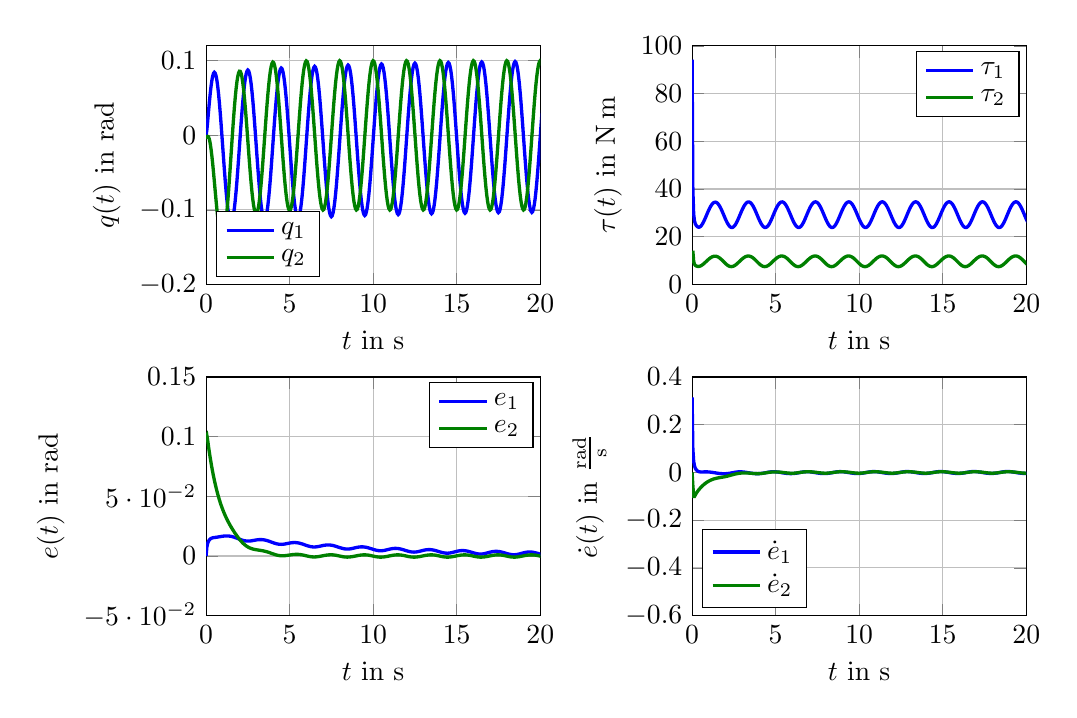
\begin{tikzpicture}

\begin{axis}[%
width=0.35\textwidth,
height=0.25\textwidth,
scale only axis,
xmin=0,
xmax=20,
xlabel={$t$ in $\mathrm{s}$},
xmajorgrids,
ymin=-0.2,
ymax=0.12,
ylabel={$q(t)$ in $\mathrm{rad}$},
ymajorgrids,
name=plot1,
legend style={at={(0.03,0.03)},anchor=south west,draw=black,fill=white,legend cell align=left}
]
\addplot [
color=blue,
solid,
line width=1.2pt
]
table[row sep=crcr]{
0 0\\
0.0457005336433737 0.00702190024651857\\
0.0957005336433737 0.0189510569534264\\
0.145700533643374 0.0317702600228906\\
0.195700533643374 0.0441799807449127\\
0.245700533643374 0.0555421782752471\\
0.295700533643374 0.0654245444159547\\
0.345700533643374 0.0734913514347467\\
0.395700533643374 0.0794805891878274\\
0.445700533643374 0.0832001049859639\\
0.495700533643374 0.084527033206208\\
0.545700533643374 0.0834071971842545\\
0.595700533643374 0.079853778099216\\
0.645700533643374 0.0739450224827181\\
0.695700533643374 0.0658208635677224\\
0.745700533643374 0.0556783969818979\\
0.795700533643374 0.0437662175578803\\
0.845700533643374 0.0303776859479665\\
0.895700533643374 0.0158432457637855\\
0.945700533643374 0.000521952188911742\\
0.995700533643375 -0.0152075983497855\\
1.04570053364337 -0.0309567295826384\\
1.09570053364336 -0.0463363203943905\\
1.14570053364336 -0.0609663932463772\\
1.19570053364335 -0.0744854384643149\\
1.24570053364335 -0.0865592635183841\\
1.29570053364334 -0.0968891664264227\\
1.34570053364334 -0.105219245478124\\
1.39570053364333 -0.111342673778848\\
1.44570053364333 -0.115106787085209\\
1.49570053364332 -0.116416857543078\\
1.54570053364331 -0.11523845454886\\
1.59570053364331 -0.111598326944249\\
1.6457005336433 -0.105583777488359\\
1.6957005336433 -0.0973405398230976\\
1.74570053364329 -0.0870692082798653\\
1.79570053364329 -0.0750203099336213\\
1.84570053364328 -0.0614881443844719\\
1.89570053364328 -0.0468035482339734\\
1.94570053364327 -0.0313257670368944\\
1.99570053364326 -0.0154336371734875\\
2.04570053364326 0.000483706301146583\\
2.09570053364325 0.0160363716950152\\
2.14570053364325 0.0308432751926231\\
2.19570053364324 0.0445415012452234\\
2.24570053364324 0.0567952366371053\\
2.29570053364323 0.067304063834293\\
2.34570053364323 0.0758104106284759\\
2.39570053364322 0.082105968590426\\
2.44570053364322 0.086036913099511\\
2.49570053364321 0.0875077833221757\\
2.5457005336432 0.0864839117775042\\
2.5957005336432 0.0829923298325364\\
2.64570053364319 0.0771211167189892\\
2.69570053364319 0.0690172038630965\\
2.74570053364318 0.0588826913101263\\
2.79570053364318 0.0469697763467891\\
2.84570053364317 0.0335744336810653\\
2.89570053364317 0.0190290197534029\\
2.94570053364316 0.00369399964392029\\
2.99570053364315 -0.0120509868559434\\
3.04570053364315 -0.0278164928136335\\
3.09570053364314 -0.0432128341404003\\
3.14570053364314 -0.0578596321366275\\
3.19570053364313 -0.0713951043324875\\
3.24570053364313 -0.0834848882166321\\
3.29570053364312 -0.0938301940224307\\
3.34570053364312 -0.102175096933822\\
3.39570053364311 -0.108312796165733\\
3.44570053364311 -0.112090688891376\\
3.4957005336431 -0.113414131484299\\
3.54570053364309 -0.112248789367252\\
3.59570053364309 -0.108621509850751\\
3.64570053364308 -0.102619689090527\\
3.69570053364308 -0.094389143509844\\
3.74570053364307 -0.084130536063843\\
3.79570053364307 -0.0720944466573809\\
3.84570053364306 -0.0585752119789341\\
3.89570053364306 -0.0439036913978795\\
3.94570053364305 -0.0284391413188094\\
3.99570053364304 -0.0125604000251834\\
4.04570053364306 0.00334340132904747\\
4.09570053364308 0.0188823777940611\\
4.14570053364309 0.0336754526317143\\
4.19570053364311 0.0473597158523159\\
4.24570053364313 0.0595993571874502\\
4.29570053364314 0.0700939591286012\\
4.34570053364316 0.0785859469907379\\
4.39570053364318 0.0848670083947626\\
4.44570053364319 0.0887833147617196\\
4.49570053364321 0.0902394029813422\\
4.54570053364323 0.0892006066665687\\
4.59570053364324 0.0856939631173371\\
4.64570053364326 0.0798075633971451\\
4.69570053364328 0.0716883571787712\\
4.74570053364329 0.061538469073738\\
4.79570053364331 0.0496101265564153\\
4.84570053364333 0.0361993389202948\\
4.89570053364334 0.0216384999744713\\
4.94570053364336 0.00628811311381088\\
4.99570053364338 -0.00947214448939626\\
5.04570053364339 -0.025252791211455\\
5.09570053364341 -0.0406641124566215\\
5.14570053364343 -0.055325704338993\\
5.19570053364344 -0.0688757652497084\\
5.24570053364346 -0.0809799198921249\\
5.29570053364348 -0.0913393719803485\\
5.34570053364349 -0.0996981960168147\\
5.39570053364351 -0.105849595676685\\
5.44570053364353 -0.109640976855182\\
5.49570053364354 -0.11097770793306\\
5.54570053364356 -0.109825468636304\\
5.59570053364358 -0.106211121947479\\
5.64570053364359 -0.100222080257753\\
5.69570053364361 -0.092004176146594\\
5.74570053364363 -0.0817580881864899\\
5.79570053364364 -0.0697344110834571\\
5.84570053364366 -0.0562274953968346\\
5.89570053364368 -0.0415682134525468\\
5.94570053364369 -0.0261158338018859\\
5.99570053364371 -0.0102492062138461\\
6.04570053364373 0.00564252718211231\\
6.09570053364374 0.0211694708524186\\
6.14570053364376 0.0359505378080248\\
6.19570053364378 0.0496228081581624\\
6.24570053364379 0.0618504621826175\\
6.29570053364381 0.0723330735494123\\
6.34570053364383 0.0808130596256062\\
6.39570053364384 0.0870821012561622\\
6.44570053364386 0.0909863645786391\\
6.49570053364388 0.092430383006765\\
6.54570053364389 0.0913794887630038\\
6.59570053364391 0.087860720052853\\
6.64570053364393 0.0819621712580674\\
6.69570053364394 0.073830797786367\\
6.74570053364396 0.0636687322833778\\
6.79570053364398 0.0517282123201955\\
6.84570053364399 0.0383052590077377\\
6.89570053364401 0.023732279268939\\
6.94570053364403 0.00836979043169746\\
6.99570053364404 -0.00740251607746312\\
7.04570053364406 -0.0231951445469725\\
7.09570053364408 -0.0386183669095894\\
7.14570053364409 -0.053291766815939\\
7.19570053364411 -0.0668535315214912\\
7.24570053364413 -0.0789692761635182\\
7.29570053364414 -0.0893401966238564\\
7.34570053364416 -0.0977103613988785\\
7.39570053364418 -0.103872970013818\\
7.4457005336442 -0.10767542604897\\
7.49570053364421 -0.109023097344854\\
7.54570053364423 -0.107881664773462\\
7.59570053364425 -0.104277994042178\\
7.64570053364426 -0.098299501726005\\
7.69570053364428 -0.0900920259189905\\
7.7457005336443 -0.0798562519034935\\
7.79570053364431 -0.0678427821474361\\
7.84570053364433 -0.0543459758712708\\
7.89570053364435 -0.039696714796906\\
7.94570053364436 -0.0242542774293365\\
7.99570053364438 -0.00839752385893951\\
8.04570053364436 0.00748439329729272\\
8.09570053364433 0.0230015680623293\\
8.1457005336443 0.0377729032627562\\
8.19570053364427 0.0514354692977987\\
8.24570053364424 0.0636534374222676\\
8.29570053364422 0.0741263731654571\\
8.34570053364419 0.0825966868289132\\
8.39570053364416 0.0888560534332125\\
8.44570053364413 0.0927506346765807\\
8.49570053364411 0.0941849610332471\\
8.54570053364408 0.0931243633663369\\
8.59570053364405 0.0895958801428775\\
8.64570053364402 0.0836876076236118\\
8.695700533644 0.0755465046620292\\
8.74570053364397 0.0653747088172646\\
8.79570053364394 0.0534244638957827\\
8.84570053364391 0.0399917983774297\\
8.89570053364388 0.0254091274641127\\
8.94570053364386 0.010036977423482\\
8.99570053364383 -0.0057449509815186\\
9.0457005336438 -0.0215471525738906\\
9.09570053364377 -0.0369798899524912\\
9.14570053364375 -0.0516627378098192\\
9.19570053364372 -0.0652338750399112\\
9.24570053364369 -0.0773589092082192\\
9.29570053364366 -0.0877390295769415\\
9.34570053364364 -0.0961182991068014\\
9.39570053364361 -0.102289912973389\\
9.44570053364358 -0.106101271667288\\
9.49570053364355 -0.107457741246851\\
9.54570053364352 -0.106325002132096\\
9.5957005336435 -0.102729920906918\\
9.64570053364347 -0.0967599163250801\\
9.69570053364344 -0.0885608299101223\\
9.74570053364341 -0.0783333515469421\\
9.79570053364339 -0.0663280893746717\\
9.84570053364336 -0.0528394092229909\\
9.89570053364333 -0.03819820020584\\
9.9457005336433 -0.0227637488265019\\
9.99570053364327 -0.00691492358665503\\
10.0457005336432 0.00895911427657843\\
10.0957005336432 0.0244684501659681\\
10.1457005336432 0.039231978494722\\
10.1957005336432 0.052886761654525\\
10.2457005336431 0.0650969634844185\\
10.2957005336431 0.0755621428583326\\
10.3457005336431 0.084024704330937\\
10.3957005336431 0.0902763182095007\\
10.445700533643 0.0941631426126643\\
10.495700533643 0.0955897056423564\\
10.545700533643 0.0945213370420588\\
10.5957005336429 0.09098507542743\\
10.6457005336429 0.0850690184605749\\
10.6957005336429 0.0769201276014295\\
10.7457005336429 0.0667405441408205\\
10.7957005336428 0.0547825166312615\\
10.8457005336428 0.0413420791737338\\
10.8957005336428 0.0267516533029729\\
10.9457005336427 0.011371772149334\\
10.9957005336427 -0.00441785632515472\\
11.0457005336427 -0.0202277196059838\\
11.0957005336427 -0.0356680730114056\\
11.1457005336426 -0.050358484196596\\
11.1957005336426 -0.0639371254338216\\
11.2457005336426 -0.0760695982367764\\
11.2957005336426 -0.0864570865202995\\
11.3457005336425 -0.0948436487154711\\
11.3957005336425 -0.101022476378101\\
11.4457005336425 -0.104840967360195\\
11.4957005336424 -0.106204486113642\\
11.5457005336424 -0.105078712514691\\
11.5957005336424 -0.101490513675985\\
11.6457005336424 -0.0955273099407635\\
11.6957005336423 -0.0873349454482596\\
11.7457005336423 -0.0771141136670782\\
11.7957005336423 -0.0651154272057752\\
11.8457005336422 -0.0516332571433589\\
11.8957005336422 -0.0369984984954958\\
11.9457005336422 -0.0215704441735484\\
11.9957005336422 -0.00572796943339754\\
12.0457005336421 0.0101397575567053\\
12.0957005336421 0.0256428152639816\\
12.1457005336421 0.0404000913318961\\
12.1957005336421 0.0540486417110121\\
12.245700533642 0.0662526242789465\\
12.295700533642 0.076711592563818\\
12.345700533642 0.0851679465083428\\
12.3957005336419 0.0914133526404982\\
12.4457005336419 0.0952939662103955\\
12.4957005336419 0.0967143134185957\\
12.5457005336419 0.0956397231081512\\
12.5957005336418 0.092097234005473\\
12.6457005336418 0.0861749448804791\\
12.6957005336418 0.0780198192589449\\
12.7457005336418 0.0678340013916406\\
12.7957005336417 0.0558697435972205\\
12.8457005336417 0.0424230844391156\\
12.8957005336417 0.027826450482158\\
12.9457005336416 0.0124403803113118\\
12.9957005336416 -0.00335541238475275\\
13.0457005336416 -0.0191714092491351\\
13.0957005336416 -0.0346178597965698\\
13.1457005336415 -0.0493143260656062\\
13.1957005336415 -0.0628989750361333\\
13.2457005336415 -0.0750374033774385\\
13.2957005336414 -0.0854307907161531\\
13.3457005336414 -0.0938231918431811\\
13.3957005336414 -0.100007795397425\\
13.4457005336414 -0.103831997096037\\
13.4957005336413 -0.105201160080623\\
13.5457005336413 -0.104080963767867\\
13.5957005336413 -0.100498275670927\\
13.6457005336413 -0.0945405173853941\\
13.6957005336412 -0.0863535351279251\\
13.7457005336412 -0.0761380252234859\\
13.7957005336412 -0.0641446038501525\\
13.8457005336411 -0.0506676462846644\\
13.8957005336411 -0.0360380522660521\\
13.9457005336411 -0.0206151198370705\\
13.9957005336411 -0.00477772966396411\\
14.045700533641 0.0110849445319212\\
14.095700533641 0.0265829756608093\\
14.145700533641 0.0413352459421351\\
14.1957005336409 0.0549788061661786\\
14.2457005336409 0.0671778094352135\\
14.2957005336409 0.0776318049958289\\
14.3457005336409 0.0860831890975874\\
14.3957005336408 0.092323625242551\\
14.4457005336408 0.0961992663843515\\
14.4957005336408 0.097614637201287\\
14.5457005336408 0.0965350658150444\\
14.5957005336407 0.0929875910394634\\
14.6457005336407 0.0870603125291712\\
14.6957005336407 0.0789001954605973\\
14.7457005336406 0.0687093864499816\\
14.7957005336406 0.0567401408260551\\
14.8457005336406 0.043288500719231\\
14.8957005336406 0.0286868967155629\\
14.9457005336405 0.0132958717612525\\
14.9957005336405 -0.002504855875491\\
15.0457005336405 -0.0183257631647369\\
15.0957005336404 -0.0337770949782522\\
15.1457005336404 -0.0484784088600398\\
15.1957005336404 -0.0620678675537844\\
15.2457005336404 -0.0742110638500121\\
15.2957005336403 -0.0846091739408136\\
15.3457005336403 -0.0930062497004918\\
15.3957005336403 -0.0991954774297624\\
15.4457005336403 -0.103024251133336\\
15.4957005336402 -0.104397932900411\\
15.5457005336402 -0.103282201776486\\
15.5957005336402 -0.0997039255924365\\
15.6457005336401 -0.0937505269440369\\
15.6957005336401 -0.0855678537092364\\
15.7457005336401 -0.0753566044985093\\
15.7957005336401 -0.0633673983469574\\
15.84570053364 -0.0498946138917815\\
15.89570053364 -0.0352691546536759\\
15.94570053364 -0.0198503227839814\\
15.9957005336399 -0.00401700328099885\\
16.04570053364 0.0118416256875924\\
16.0957005336401 0.0273356325826446\\
16.1457005336401 0.0420838952808282\\
16.1957005336402 0.0557234604410008\\
16.2457005336402 0.0679184773423806\\
16.2957005336403 0.0783684918040017\\
16.3457005336404 0.0868158971190211\\
16.3957005336404 0.0930523543673101\\
16.4457005336405 0.0969240146642405\\
16.4957005336406 0.0983354014695578\\
16.5457005336406 0.0972518423274004\\
16.5957005336407 0.093700376121342\\
16.6457005336407 0.0877691032137921\\
16.6957005336408 0.0796049901019318\\
16.7457005336409 0.0694101852948256\\
16.7957005336409 0.057436946529952\\
16.845700533641 0.0439813187922553\\
16.895700533641 0.0293757358859924\\
16.9457005336411 0.0139807442478749\\
16.9957005336412 -0.00182393418844499\\
17.0457005336412 -0.017648772652528\\
17.0957005336413 -0.0331040122994488\\
17.1457005336413 -0.0478092070750812\\
17.1957005336414 -0.0614025163315573\\
17.2457005336415 -0.073549529753798\\
17.2957005336415 -0.0839514207837571\\
17.3457005336416 -0.0923522389601451\\
17.3957005336417 -0.0985451687111079\\
17.4457005336417 -0.10237760266976\\
17.4957005336418 -0.10375490208219\\
17.5457005336418 -0.102642745696265\\
17.5957005336419 -0.0990680015968989\\
17.645700533642 -0.0931180931804217\\
17.695700533642 -0.0849388696547608\\
17.7457005336421 -0.0747310314602307\\
17.7957005336421 -0.0627451999194168\\
17.8457005336422 -0.0492757563601025\\
17.8957005336423 -0.0346536073307871\\
17.9457005336423 -0.0192380582723192\\
17.9957005336424 -0.00340799765135309\\
18.0457005336424 0.0124473928046753\\
18.0957005336425 0.0279381779945308\\
18.1457005336426 0.0426832323182477\\
18.1957005336426 0.0563195991273337\\
18.2457005336427 0.0685114246405998\\
18.2957005336428 0.0789582519333434\\
18.3457005336428 0.0874024719321843\\
18.3957005336429 0.0936357437781102\\
18.4457005336429 0.0975042171150319\\
18.495700533643 0.0989124144272714\\
18.5457005336431 0.0978256627966125\\
18.5957005336431 0.094271001162363\\
18.6457005336432 0.0883365304533649\\
18.6957005336432 0.0801692182238687\\
18.7457005336433 0.0699712144979268\\
18.7957005336434 0.057994778941003\\
18.8457005336434 0.0445359588229062\\
18.8957005336435 0.0299271905239348\\
18.9457005336435 0.0145290232749038\\
18.9957005336436 -0.00127881805630114\\
19.0457005336437 -0.0171068037048122\\
19.0957005336437 -0.032565171850239\\
19.1457005336438 -0.0472734735578091\\
19.1957005336439 -0.0608698654643028\\
19.2457005336439 -0.0730199347681469\\
19.295700533644 -0.0834248527093405\\
19.345700533644 -0.0918286669565028\\
19.3957005336441 -0.0980245604383898\\
19.4457005336442 -0.101859924689835\\
19.4957005336442 -0.103240120281798\\
19.5457005336443 -0.10213082572379\\
19.5957005336443 -0.0985589093040984\\
19.6457005336444 -0.0926117950600316\\
19.6957005336445 -0.0844353332644007\\
19.7457005336445 -0.074230225822628\\
19.7957005336446 -0.06224709588881\\
19.8457005336446 -0.0487803269449543\\
19.8957005336447 -0.0341608279637345\\
19.9457005336448 -0.0187479070196439\\
19.9957005336448 -0.00292045535610446\\
20.0457005336449 0.0129323424495731\\
20.095700533645 0.0284205484444812\\
20.145700533645 0.0431630342454556\\
20.1957005336451 0.0567968405563859\\
20.2457005336451 0.068986111146198\\
20.2957005336452 0.0794303868938399\\
20.3457005336453 0.0878720568315542\\
20.3957005336453 0.0941027785482943\\
20.4457005336454 0.0979687005100989\\
20.4957005336454 0.0993743444204744\\
20.5457005336455 0.0982850369910721\\
20.5957005336456 0.0947278172057667\\
20.6457005336456 0.0887907864467544\\
20.6957005336457 0.0806209131143768\\
20.7457005336457 0.0704203484453372\\
20.7957005336458 0.0584413536483656\\
20.8457005336459 0.0449799778222463\\
20.8957005336459 0.030368659409382\\
20.945700533646 0.0149679498773037\\
20.9957005336461 -0.000842423557151451\\
21.0457005336461 -0.0166729287319167\\
21.0957005336462 -0.0321338014445247\\
21.1457005336462 -0.0468445904539803\\
21.1957005336463 -0.0604434502231251\\
21.2457005336464 -0.072595965959631\\
21.2957005336464 -0.0830033071405202\\
21.3457005336465 -0.0914095199371147\\
21.3957005336465 -0.097607786077662\\
21.4457005336466 -0.101445496217633\\
21.4957005336467 -0.10282801038743\\
21.5457005336467 -0.10172100690572\\
21.5957005336468 -0.0981513542236298\\
21.6457005336468 -0.0922064768916854\\
21.6957005336469 -0.0840322260353179\\
21.745700533647 -0.0738293047330025\\
21.795700533647 -0.0618483376052308\\
21.8457005336471 -0.0483837098587556\\
21.8957005336472 -0.0337663324070918\\
21.9457005336472 -0.0183555154332398\\
21.9957005336473 -0.00253015240366774\\
22.0457005336473 0.0133205698227834\\
22.0957005336474 0.0288067110102827\\
22.1457005336475 0.0435471405476015\\
22.1957005336475 0.0571788970191406\\
22.2457005336476 0.0693661222326587\\
22.2957005336476 0.079808355308919\\
22.3457005336477 0.0882479837637246\\
22.3957005336478 0.0944766639436408\\
22.4457005336478 0.098340543371832\\
22.4957005336479 0.099744143126763\\
22.5457005336479 0.0986527896237806\\
22.595700533648 0.0950935218824055\\
22.6457005336481 0.0891544416477021\\
22.6957005336481 0.0809825179972586\\
22.7457005336482 0.0707799031384569\\
22.7957005336483 0.0587988595153742\\
22.8457005336483 0.0453354376908727\\
22.8957005336484 0.0307220777580814\\
22.9457005336484 0.0153193329750704\\
22.9957005336485 -0.000493067560900889\\
23.0457005336486 -0.0163255897686814\\
23.0957005336486 -0.0317884675387886\\
23.1457005336487 -0.0465012477839045\\
23.1957005336487 -0.0601020832264217\\
23.2457005336488 -0.0722565574801942\\
23.2957005336489 -0.0826658386107674\\
23.3457005336489 -0.0910739715906819\\
23.395700533649 -0.0972741371870129\\
23.445700533649 -0.101113725351179\\
23.4957005336491 -0.102498095680787\\
23.5457005336492 -0.101392926341712\\
23.5957005336492 -0.0978250859154651\\
23.6457005336493 -0.0918819993634822\\
23.6957005336494 -0.0837095184938432\\
23.7457005336494 -0.0735083473242134\\
23.7957005336495 -0.0615291116491206\\
23.8457005336495 -0.0480661980561764\\
23.8957005336496 -0.0334505190127412\\
23.9457005336497 -0.0180413863898677\\
23.9957005336497 -0.00221769543374737\\
24.0457005336498 0.0136313651702649\\
24.0957005336498 0.0291158533587376\\
24.1457005336499 0.0438546367367865\\
24.19570053365 0.0574847521920996\\
24.24570053365 0.0696703399624842\\
24.2957005336501 0.080110937761258\\
24.3457005336501 0.0885489318903085\\
24.3957005336502 0.0947759777016697\\
24.4457005336503 0.0986382219637351\\
24.4957005336503 0.10004018525462\\
24.5457005336504 0.0989471937524678\\
24.5957005336505 0.0953862865053167\\
24.6457005336505 0.0894455655486828\\
24.6957005336506 0.0812720005022648\\
24.7457005336506 0.0710677443504506\\
24.7957005336507 0.0590850605261998\\
24.8457005336508 0.0456200007643704\\
24.8957005336508 0.0310050064795202\\
24.9457005336509 0.0156006323630915\\
24.9957005336509 -0.000213390982306023\\
25.045700533651 -0.0160475279391973\\
25.0957005336511 -0.031512010871414\\
25.1457005336511 -0.0462263852135186\\
25.1957005336512 -0.0598288022945245\\
25.2457005336512 -0.0719848444522814\\
25.2957005336513 -0.0823956786222996\\
25.3457005336514 -0.09080534881736\\
25.3957005336514 -0.0970070350350074\\
25.4457005336515 -0.10084812666298\\
25.4957005336516 -0.102233982952384\\
25.5457005336516 -0.101130281946766\\
25.5957005336517 -0.0975638923320312\\
25.6457005336517 -0.0916222393986054\\
25.6957005336518 -0.0834511755011152\\
25.7457005336519 -0.0732514054091593\\
25.7957005336519 -0.061273555857211\\
25.845700533652 -0.0478120145383996\\
25.895700533652 -0.0331976951640808\\
25.9457005336521 -0.0177899109567307\\
25.9957005336522 -0.00196755858733534\\
26.0457005336522 0.0138801717965154\\
26.0957005336523 0.0293633366683037\\
26.1457005336523 0.0441008022052569\\
26.1957005336524 0.0577296039367913\\
26.2457005336525 0.0699138808439311\\
26.2957005336525 0.0803531695133112\\
26.3457005336526 0.0887898552750663\\
26.3957005336527 0.0950155926850998\\
26.4457005336527 0.0988765279076057\\
26.4957005336528 0.100277181120162\\
26.5457005336528 0.0991828783110246\\
26.5957005336529 0.0956206585510463\\
26.645700533653 0.089678624108238\\
26.695700533653 0.0815037450362461\\
26.7457005336531 0.0712981749414444\\
26.7957005336531 0.0593141780483923\\
26.8457005336532 0.0458478070301419\\
26.8957005336533 0.0312315043590794\\
26.9457005336533 0.0158258258741032\\
26.9957005336534 1.0503382914124e-05\\
27.0457005336534 -0.0158249262671102\\
27.0957005336535 -0.0312906942176\\
27.1457005336536 -0.0460063447197823\\
27.1957005336536 -0.0596100279871634\\
27.2457005336537 -0.071767325336043\\
27.2957005336538 -0.0821794027972341\\
27.3457005336538 -0.0905903036151369\\
27.3957005336539 -0.0967932071712076\\
27.4457005336539 -0.100635502401901\\
27.495700533654 -0.102022548280911\\
27.5457005336541 -0.100920022753853\\
27.5957005336541 -0.0973547945902126\\
27.6457005336542 -0.0914142893438111\\
27.6957005336542 -0.083244359806846\\
27.7457005336543 -0.0730457113509167\\
27.7957005336544 -0.0610689714630138\\
27.8457005336544 -0.0476085287213322\\
27.8957005336545 -0.0329952978331475\\
27.9457005336545 -0.0175885931028492\\
27.9957005336546 -0.00176731234206425\\
28.0457005336547 0.0140793531310156\\
28.0957005336547 0.0295614586186014\\
28.1457005336548 0.0442978691548375\\
28.1957005336549 0.0579256191817985\\
28.2457005336549 0.0701088466744206\\
28.295700533655 0.0805470873174048\\
28.345700533655 0.0889827256629812\\
28.3957005336551 0.0952074156297396\\
28.4457005336552 0.0990673028982034\\
28.4957005336552 0.100466907325315\\
28.5457005336553 0.0993715547473143\\
28.5957005336553 0.0958082842533143\\
28.6457005336554 0.0898651982974309\\
28.6957005336555 0.081689267280682\\
28.7457005336555 0.0714826453073411\\
28.7957005336556 0.0594975972356499\\
28.8457005336556 0.0460301764896996\\
28.8957005336557 0.0314128263886932\\
28.9457005336558 0.0160061036901038\\
28.9957005336558 0.000189741166354719\\
29.0457005336559 -0.0156467233505809\\
29.095700533656 -0.0311135200238939\\
29.145700533656 -0.045830192157477\\
29.1957005336561 -0.0594348890717953\\
29.2457005336561 -0.0715931912653199\\
29.2957005336562 -0.0820062640445797\\
29.3457005336563 -0.0904181500388196\\
29.3957005336563 -0.0966220281362622\\
29.4457005336564 -0.100465286912068\\
29.4957005336564 -0.10185328511784\\
29.5457005336565 -0.100751700620789\\
29.5957005336566 -0.097187402257318\\
29.6457005336566 -0.0912478157921244\\
29.6957005336567 -0.0830787943677231\\
29.7457005336567 -0.0728810438376702\\
29.7957005336568 -0.0609051922914111\\
29.8457005336569 -0.0474456290157063\\
29.8957005336569 -0.0328332695151387\\
29.945700533657 -0.017427428960242\\
29.9957005336571 -0.00160700607579487\\
30.0457005336571 0.0142388068828814\\
30.0957005336572 0.0297200642803401\\
30.1457005336572 0.0444556302356416\\
30.1957005336573 0.0580825383204054\\
30.2457005336574 0.0702649257041644\\
30.2957005336574 0.0807023273495993\\
30.3457005336575 0.0891371271862107\\
30.3957005336575 0.0953609786224066\\
30.4457005336576 0.0992200269515229\\
30.4957005336577 0.100618791773825\\
30.5457005336577 0.0995225988038613\\
30.5957005336578 0.0959584871453556\\
30.6457005336578 0.0900145594013994\\
30.6957005336579 0.0818377862510822\\
30.745700533658 0.0716303221972505\\
30.795700533658 0.0596444326054188\\
30.8457005336581 0.0461761715009006\\
30.8957005336582 0.0315579828807988\\
30.9457005336582 0.0161504242379359\\
30.9957005336583 0.0003332291170346\\
31.0457005336583 -0.0155040638617184\\
31.0957005336584 -0.0309716840782217\\
31.1457005336585 -0.0456891740779719\\
31.1957005336585 -0.0592946824664973\\
31.2457005336586 -0.071453789087541\\
31.2957005336586 -0.0818676586677892\\
31.3457005336587 -0.0902803333440073\\
31.3957005336588 -0.0964849916095454\\
31.4457005336588 -0.100329021750319\\
31.4957005336589 -0.101717782340128\\
31.5457005336589 -0.100616951183419\\
31.595700533659 -0.0970533971701669\\
31.6457005336591 -0.091114546233895\\
31.6957005336591 -0.0829462517975779\\
31.7457005336592 -0.0727492201006174\\
31.7957005336593 -0.0607740797147705\\
31.8457005336593 -0.0473152204940559\\
31.8957005336594 -0.0327035585813545\\
31.9457005336594 -0.0172984098406022\\
31.9957005336595 -0.00147867372760714\\
32.0457005336594 0.0143664567520889\\
32.0957005336593 0.029847035212403\\
32.1457005336592 0.0445819250398366\\
32.195700533659 0.0582081591091813\\
32.2457005336589 0.070389873945221\\
32.2957005336588 0.0808266039326408\\
32.3457005336587 0.0892607325024314\\
32.3957005336586 0.0954839126545887\\
32.4457005336585 0.0993422893724961\\
32.4957005336583 0.100740382050942\\
32.5457005336582 0.0996435163070534\\
32.5957005336581 0.0960787312562465\\
32.645700533658 0.0901341296208648\\
32.6957005336579 0.0819566823025932\\
32.7457005336578 0.0717485441233389\\
32.7957005336576 0.0597619808546938\\
32.8457005336575 0.0462930470032613\\
32.8957005336574 0.0316741871088191\\
32.9457005336573 0.0162659592528592\\
32.9957005336572 0.000448097598356601\\
33.0457005336571 -0.0153898586035043\\
33.0957005336569 -0.0308581381055598\\
33.1457005336568 -0.0455762828461706\\
33.1957005336567 -0.0591824408585165\\
33.2457005336566 -0.0713421914621891\\
33.2957005336565 -0.0817566989196707\\
33.3457005336564 -0.0901700049734606\\
33.3957005336562 -0.0963752878007815\\
33.4457005336561 -0.100219935455983\\
33.495700533656 -0.101609306370518\\
33.5457005336559 -0.100509078298576\\
33.5957005336558 -0.096946120173019\\
33.6457005336557 -0.0910078580625212\\
33.6957005336555 -0.0828401456145793\\
33.7457005336554 -0.0726436893774855\\
33.7957005336553 -0.060669118309114\\
33.8457005336552 -0.047210822717604\\
33.8957005336551 -0.0325997192568272\\
33.945700533655 -0.0171951243458224\\
33.9957005336548 -0.00137593802562132\\
34.0457005336547 0.0144686460976501\\
34.0957005336546 0.0299486810369901\\
34.1457005336545 0.0446830295924518\\
34.1957005336544 0.0583087240809851\\
34.2457005336543 0.070489900511225\\
34.2957005336541 0.080926092805146\\
34.345700533654 0.0893596839946606\\
34.3957005336539 0.0955823267528122\\
34.4457005336538 0.0994401658148511\\
34.4957005336537 0.100837720411068\\
34.5457005336536 0.0997403160805943\\
34.5957005336534 0.0961749919481971\\
34.6457005336533 0.0902298508316763\\
34.6957005336532 0.0820518638109033\\
34.7457005336531 0.0718431859631954\\
34.795700533653 0.0598560833852168\\
34.8457005336529 0.0463866109688547\\
34.8957005336528 0.0317672136883147\\
34.9457005336526 0.0163584500963395\\
34.9957005336525 0.000540054850841372\\
35.0457005336524 -0.0152984322918518\\
35.0957005336523 -0.0307672395825804\\
35.1457005336522 -0.0454859084736575\\
35.1957005336521 -0.0590925865400625\\
35.2457005336519 -0.0712528526817683\\
35.2957005336518 -0.0816678707896291\\
35.3457005336517 -0.0900816822905041\\
35.3957005336516 -0.0962874651085312\\
35.4457005336515 -0.100132607112672\\
35.4957005336514 -0.101522466620416\\
35.5457005336512 -0.100422721345718\\
35.5957005336511 -0.0968602402557701\\
35.645700533651 -0.0909224495274424\\
35.6957005336509 -0.0827552029879759\\
35.7457005336508 -0.0725592074329494\\
35.7957005336507 -0.060585092129348\\
35.8457005336505 -0.0471272477488625\\
35.8957005336504 -0.0325165913544432\\
35.9457005336503 -0.0171124398095204\\
35.9957005336502 -0.00129369362362872\\
36.0457005336501 0.0145504531163073\\
36.09570053365 0.0300300529422227\\
36.1457005336498 0.0447639681846951\\
36.1957005336497 0.0583892307141005\\
36.2457005336496 0.0705699761258775\\
36.2957005336495 0.0810057379715851\\
36.3457005336494 0.0894388989636602\\
36.3957005336493 0.0956611115134099\\
36.4457005336491 0.0995185201574453\\
36.495700533649 0.10091564399437\\
36.5457005336489 0.0998178085008764\\
36.5957005336488 0.0962520528092141\\
36.6457005336487 0.0903064798135962\\
36.6957005336486 0.0821280607365346\\
36.7457005336484 0.071918950859808\\
36.7957005336483 0.0599314165403088\\
36.8457005336482 0.0464615129783549\\
36.8957005336481 0.0318416854959255\\
36.945700533648 0.0164324930230169\\
36.9957005336479 0.000613670613757952\\
37.0457005336477 -0.015225241571134\\
37.0957005336476 -0.0306944713806278\\
37.1457005336475 -0.0454135598779311\\
37.1957005336474 -0.0590206542712089\\
37.2457005336473 -0.0711813331245056\\
37.2957005336472 -0.0815967600311645\\
37.345700533647 -0.0900109761653553\\
37.3957005336469 -0.0962171592486051\\
37.4457005336468 -0.10006269700146\\
37.4957005336467 -0.101452947650173\\
37.5457005336466 -0.100353588876487\\
37.5957005336465 -0.0967914896750788\\
37.6457005336463 -0.0908540763094338\\
37.6957005336462 -0.0826872027506888\\
37.7457005336461 -0.07249157599239\\
37.795700533646 -0.0605178255489831\\
37.8457005336459 -0.0470603423832021\\
37.8957005336458 -0.0324500438854862\\
37.9457005336456 -0.0170462472750235\\
37.9957005336455 -0.00122785343640826\\
38.0457005336454 0.0146159431585338\\
38.0957005336453 0.0300951946566256\\
38.1457005336452 0.0448287630126102\\
38.1957005336451 0.058453679739363\\
38.2457005336449 0.0706340801015438\\
38.2957005336448 0.0810694973541802\\
38.3457005336447 0.0895023139539572\\
38.3957005336446 0.0957241821026524\\
38.4457005336445 0.0995812461778592\\
38.4957005336444 0.10097802517276\\
38.5457005336442 0.0998798445140601\\
38.5957005336441 0.0963137433399981\\
38.645700533644 0.0903678246059559\\
38.6957005336439 0.0821890596486317\\
38.7457005336438 0.0719796039134799\\
38.7957005336437 0.0599917239657126\\
38.8457005336435 0.0465214752525561\\
38.8957005336434 0.0319013033743939\\
38.9457005336433 0.0164917675632273\\
38.9957005336432 0.000672603190372969\\
39.0457005336431 -0.015166649259721\\
39.095700533643 -0.0306362173143068\\
39.1457005336428 -0.0453556417250939\\
39.1957005336427 -0.0589630694065935\\
39.2457005336426 -0.071124078653921\\
39.2957005336425 -0.081539832822245\\
39.3457005336424 -0.0899543728834426\\
39.3957005336423 -0.0961608763968377\\
39.4457005336421 -0.10000673096416\\
39.495700533642 -0.101397294738622\\
39.5457005336419 -0.10029824537618\\
39.5957005336418 -0.0967364518935087\\
39.6457005336417 -0.0907993406234358\\
39.6957005336416 -0.0826327656522938\\
39.7457005336414 -0.072437434132112\\
39.7957005336413 -0.0604639757754415\\
39.8457005336412 -0.0470067817780111\\
39.8957005336411 -0.0323967697924311\\
39.945700533641 -0.0169932573226912\\
39.9957005336409 -0.00117514555363815\\
40.0457005336407 0.0146683707347714\\
40.0957005336406 0.0301473433810616\\
40.1457005336405 0.0448806340391039\\
40.1957005336404 0.0585052739355806\\
40.2457005336403 0.0706853980703496\\
40.2957005336402 0.0811205394610538\\
40.34570053364 0.0895530803596392\\
40.3957005336399 0.095774672800147\\
40.4457005336398 0.0996314610328698\\
40.4957005336397 0.101027963966596\\
40.5457005336396 0.0999295069880126\\
40.5957005336395 0.0963631292401514\\
40.6457005336393 0.0904169337273601\\
40.6957005336392 0.0822378918777449\\
40.7457005336391 0.0720281592677868\\
40.795700533639 0.0600400026294637\\
40.8457005336389 0.0465694776076596\\
40.8957005336388 0.0319490300256302\\
40.9457005336387 0.0165392193571435\\
40.9957005336385 0.000719781227436938\\
41.0457005336384 -0.0151197436198807\\
41.0957005336383 -0.0305895824545129\\
41.1457005336382 -0.0453092757788001\\
41.1957005336381 -0.0589169702721689\\
41.245700533638 -0.0710782440144426\\
41.2957005336378 -0.0814942601701182\\
41.3457005336377 -0.0899090595491256\\
41.3957005336376 -0.0961158195809356\\
41.4457005336375 -0.0999619277721577\\
41.4957005336374 -0.101352742217531\\
41.5457005336373 -0.100253940552365\\
41.5957005336371 -0.0966923918109459\\
41.645700533637 -0.0907555223816126\\
41.6957005336369 -0.0825891864429169\\
41.7457005336368 -0.0723940912737612\\
41.7957005336367 -0.0604208667452895\\
41.8457005336366 -0.0469639042397544\\
41.8957005336364 -0.0323541216196467\\
41.9457005336363 -0.0169508366169527\\
41.9957005336362 -0.00113295065688496\\
42.0457005336361 0.0147103412339274\\
42.095700533636 0.0301890906472021\\
42.1457005336359 0.0449221589959503\\
42.1957005336357 0.058546577277745\\
42.2457005336356 0.0707264802804594\\
42.2957005336355 0.0811614008317004\\
42.3457005336354 0.0895937210195122\\
42.3957005336353 0.0958150927436559\\
42.4457005336352 0.0996716601525145\\
42.495700533635 0.101067942087315\\
42.5457005336349 0.0999692639027061\\
42.5957005336348 0.0964026647455559\\
42.6457005336347 0.0904562476594092\\
42.6957005336346 0.0822769841455463\\
42.7457005336345 0.0720670298853379\\
42.7957005336343 0.0600786517442628\\
42.8457005336342 0.0466079055254364\\
42.8957005336341 0.0319872372305316\\
42.945700533634 0.016577206526859\\
42.9957005336339 0.000757549242930502\\
43.0457005336338 -0.0150821936701766\\
43.0957005336336 -0.0305522492759864\\
43.1457005336335 -0.0452721578772077\\
43.1957005336334 -0.0588800659650705\\
43.2457005336333 -0.0710415514470456\\
43.2957005336332 -0.0814577773349872\\
43.3457005336331 -0.0898727843091771\\
43.3957005336329 -0.0960797496951315\\
43.4457005336328 -0.0999260609233099\\
43.4957005336327 -0.101317076041639\\
43.5457005336326 -0.100218472668899\\
43.5957005336325 -0.0966571198534739\\
43.6457005336324 -0.0907204440281407\\
43.6957005336322 -0.0825542994452768\\
43.7457005336321 -0.0723593934853522\\
43.795700533632 -0.0603863561464718\\
43.8457005336319 -0.0469295789602085\\
43.8957005336318 -0.0323199799570721\\
43.9457005336317 -0.0169168770515704\\
43.9957005336315 -0.00109917186133951\\
44.0457005336314 0.0147439403895196\\
44.0957005336313 0.0302225110951456\\
44.1457005336312 0.0449554014757307\\
44.1957005336311 0.0585796423454362\\
44.245700533631 0.070759368322433\\
44.2957005336308 0.0811941120821962\\
44.3457005336307 0.0896262555815596\\
44.3957005336306 0.0958474506127871\\
44.4457005336305 0.0997038412426783\\
44.4957005336304 0.101099946258373\\
44.5457005336303 0.100001090988873\\
44.5957005336301 0.0964343145841131\\
44.64570053363 0.0904877201190173\\
44.6957005336299 0.0823082791534426\\
44.7457005336298 0.0720981474527266\\
44.7957005336297 0.0601095919892196\\
44.8457005336296 0.0466386686927061\\
44.8957005336294 0.0320178237076881\\
44.9457005336293 0.0166076168564147\\
44.9957005336292 0.000787784130126391\\
45.0457005336291 -0.0150521333540118\\
45.095700533629 -0.0305223624944684\\
45.1457005336289 -0.0452424434341381\\
45.1957005336287 -0.0588505225135899\\
45.2457005336286 -0.0710121775023183\\
45.2957005336285 -0.0814285712899784\\
45.3457005336284 -0.0898437444530619\\
45.3957005336283 -0.0960508742338626\\
45.4457005336282 -0.0998973480018779\\
45.495700533628 -0.101288523767557\\
45.5457005336279 -0.100190079136447\\
45.5957005336278 -0.0966288831682166\\
45.6457005336277 -0.0906923623312166\\
45.6957005336276 -0.0825263709369245\\
45.7457005336275 -0.0723316164471192\\
45.7957005336273 -0.0603587289615431\\
45.8457005336272 -0.0469021001313066\\
45.8957005336271 -0.0322926481214256\\
45.945700533627 -0.0168896909925246\\
45.9957005336269 -0.00107213051628269\\
46.0457005336268 0.0147708379251143\\
46.0957005336266 0.0302492655676346\\
46.1457005336265 0.0449820134771108\\
46.1957005336264 0.0586061123208752\\
46.2457005336263 0.0707856965812448\\
46.2957005336262 0.0812202988119065\\
46.3457005336261 0.0896523008646542\\
46.3957005336259 0.0958733544456957\\
46.4457005336258 0.0997296035565187\\
46.4957005336257 0.101125566940963\\
46.5457005336256 0.100026569907497\\
46.5957005336255 0.0964596516085123\\
46.6457005336254 0.0905129151440485\\
46.6957005336252 0.0823333321208553\\
46.7457005336251 0.072123058371488\\
46.795700533625 0.0601343609538502\\
46.8457005336249 0.0466632958991295\\
46.8957005336248 0.0320423094661672\\
46.9457005336247 0.0166319616012464\\
46.9957005336246 0.000811988425878647\\
47.0457005336244 -0.0150280688098113\\
47.0957005336243 -0.0304984368721577\\
47.1457005336242 -0.0452186557761167\\
47.1957005336241 -0.058826871741646\\
47.245700533624 -0.0709886624277829\\
47.2957005336239 -0.081405190626356\\
47.3457005336237 -0.089820496830767\\
47.3957005336236 -0.0960277582166856\\
47.4457005336235 -0.0998743621048044\\
47.4957005336234 -0.10126566647557\\
47.5457005336233 -0.100167348923933\\
47.5957005336232 -0.0966062785185961\\
47.645700533623 -0.0906698817563877\\
47.6957005336229 -0.0825040129960963\\
47.7457005336228 -0.0723093797645918\\
47.7957005336227 -0.060336612242981\\
47.8457005336226 -0.0468801021780689\\
47.8957005336225 -0.0322707678425495\\
47.9457005336223 -0.0168679274140192\\
47.9957005336222 -0.00105048278747541\\
48.0457005336221 0.0147923705283427\\
48.095700533622 0.0302706836427809\\
48.1457005336219 0.0450033174981004\\
48.1957005336218 0.0586273026440908\\
48.2457005336216 0.0708067734543117\\
48.2957005336215 0.0812412623849534\\
48.3457005336214 0.0896731512037204\\
48.3957005336213 0.0958940915479279\\
48.4457005336212 0.0997502273667782\\
48.4957005336211 0.101146077369447\\
48.5457005336209 0.100046966847963\\
48.5957005336208 0.0964799349566828\\
48.6457005336207 0.0905330848157523\\
48.6957005336206 0.0823533880694587\\
48.7457005336205 0.0721430006041665\\
48.7957005336204 0.0601541895462673\\
48.8457005336202 0.0466830110081247\\
48.8957005336201 0.0320619113401127\\
48.94570053362 0.0166514505878083\\
48.9957005336199 0.000831364977009709\\
49.0457005336198 -0.0150088041357182\\
49.0957005336197 -0.0304792834109308\\
49.1457005336195 -0.0451996127611632\\
49.1957005336194 -0.0588079383098183\\
49.2457005336193 -0.0709698376275067\\
49.2957005336192 -0.0813864734277417\\
49.3457005336191 -0.0898018861374068\\
49.395700533619 -0.096009252878835\\
49.4457005336188 -0.0998559609336472\\
49.4957005336187 -0.10124736825827\\
49.5457005336186 -0.100149152439171\\
49.5957005336185 -0.0965881825522845\\
49.6457005336184 -0.0906518851172332\\
49.6957005336183 -0.0824861145306805\\
49.7457005336181 -0.0722915783716034\\
49.795700533618 -0.0603189068862441\\
49.8457005336179 -0.0468624918980146\\
49.8957005336178 -0.0322532517658092\\
49.9457005336177 -0.0168505047608654\\
49.9957005336176 -0.00103315287690166\\
};
\addlegendentry{$q_1$};

\addplot [
color=green!50!black,
solid,
line width=1.2pt
]
table[row sep=crcr]{
0 0\\
0.0457005336433737 -0.00216726495678186\\
0.0957005336433737 -0.00137691230800364\\
0.145700533643374 -0.00209866253861438\\
0.195700533643374 -0.00524589935220222\\
0.245700533643374 -0.0107315865454966\\
0.295700533643374 -0.0182731674366757\\
0.345700533643374 -0.0275442576128161\\
0.395700533643374 -0.038194835736617\\
0.445700533643374 -0.0498540527358989\\
0.495700533643374 -0.0621348240158785\\
0.545700533643374 -0.0746410983605356\\
0.595700533643374 -0.0869765552348893\\
0.645700533643374 -0.0987538262149619\\
0.695700533643374 -0.109603707463751\\
0.745700533643374 -0.119184012674409\\
0.795700533643374 -0.127187795834037\\
0.845700533643374 -0.13335071570149\\
0.895700533643374 -0.137457347258713\\
0.945700533643374 -0.139346278980813\\
0.995700533643375 -0.138913870567062\\
1.04570053364337 -0.136116583274211\\
1.09570053364336 -0.130971833036656\\
1.14570053364336 -0.123557354014155\\
1.19570053364335 -0.11400909620904\\
1.24570053364335 -0.102517714782831\\
1.29570053364334 -0.0893237403784681\\
1.34570053364334 -0.0747115489786797\\
1.39570053364333 -0.0590022765008763\\
1.44570053364333 -0.0425458472702531\\
1.49570053364332 -0.0257123064021801\\
1.54570053364331 -0.00888266346283\\
1.59570053364331 0.00756053208303303\\
1.6457005336433 0.0232426548963246\\
1.6957005336433 0.0378062758500788\\
1.74570053364329 0.0509200141321732\\
1.79570053364329 0.0622867508953691\\
1.84570053364328 0.0716510016074466\\
1.89570053364328 0.0788052654099831\\
1.94570053364327 0.0835951956935932\\
1.99570053364326 0.0859234657712412\\
2.04570053364326 0.0857522359443746\\
2.09570053364325 0.0831041624060504\\
2.14570053364325 0.0780619234090583\\
2.19570053364324 0.0707662731795983\\
2.24570053364324 0.0614126685530277\\
2.29570053364323 0.0502465467411974\\
2.34570053364323 0.0375573645808437\\
2.39570053364322 0.0236715396456526\\
2.44570053364322 0.00894446126335054\\
2.49570053364321 -0.00624823582426869\\
2.5457005336432 -0.0215199214358604\\
2.5957005336432 -0.0364825134701515\\
2.64570053364319 -0.0507560741246017\\
2.69570053364319 -0.0639782137682277\\
2.74570053364318 -0.0758130605131538\\
2.79570053364318 -0.0859595642488862\\
2.84570053364317 -0.0941589220826426\\
2.89570053364317 -0.100200937050552\\
2.94570053364316 -0.103929152430159\\
2.99570053364315 -0.105244638473138\\
3.04570053364315 -0.104108345251801\\
3.09570053364314 -0.100541973030172\\
3.14570053364314 -0.0946273488417497\\
3.19570053364313 -0.0865043338355373\\
3.24570053364313 -0.0763673198406027\\
3.29570053364312 -0.064460405179996\\
3.34570053364312 -0.0510713688908504\\
3.39570053364311 -0.0365245890768939\\
3.44570053364311 -0.021173074960174\\
3.4957005336431 -0.00538980298912972\\
3.54570053364309 0.0104414353981585\\
3.59570053364309 0.0259354537085771\\
3.64570053364308 0.0407151292327434\\
3.69570053364308 0.0544206693999959\\
3.74570053364307 0.0667184576863679\\
3.79570053364307 0.0773092607323953\\
3.84570053364306 0.085935593973637\\
3.89570053364306 0.0923880642489862\\
3.94570053364305 0.0965105337430026\\
3.99570053364304 0.098203979274144\\
4.04570053364306 0.0974289533301434\\
4.09570053364308 0.0942065873750154\\
4.14570053364309 0.0886181129088999\\
4.19570053364311 0.0808029107866124\\
4.24570053364313 0.0709551337677238\\
4.29570053364314 0.0593189806741064\\
4.34570053364316 0.0461827324416483\\
4.39570053364318 0.0318716903605809\\
4.44570053364319 0.0167401844400243\\
4.49570053364321 0.00116284452307133\\
4.54570053364323 -0.0144746522281459\\
4.59570053364324 -0.0297851274680507\\
4.64570053364326 -0.0443895006231025\\
4.69570053364328 -0.0579261956263291\\
4.74570053364329 -0.0700601134387189\\
4.79570053364331 -0.0804909390513427\\
4.84570053364333 -0.0889605698209543\\
4.89570053364334 -0.0952594769085209\\
4.94570053364336 -0.0992318420662533\\
4.99570053364338 -0.100779346529678\\
5.04570053364339 -0.0998635256754264\\
5.09570053364341 -0.0965066408534507\\
5.14570053364343 -0.0907910571010966\\
5.19570053364344 -0.0828571513466698\\
5.24570053364346 -0.072899809611419\\
5.29570053364348 -0.0611636033041116\\
5.34570053364349 -0.0479367638264329\\
5.39570053364351 -0.0335441012699549\\
5.44570053364353 -0.0183390368160046\\
5.49570053364354 -0.00269493922851509\\
5.54570053364356 0.0130040269402585\\
5.59570053364358 0.0283723207743441\\
5.64570053364359 0.0430324832551204\\
5.69570053364361 0.056624402978299\\
5.74570053364363 0.0688141613759568\\
5.79570053364364 0.0793022391152483\\
5.84570053364366 0.0878308809915981\\
5.89570053364368 0.0941904377949203\\
5.94570053364369 0.09822452951636\\
5.99570053364371 0.0998339039165373\\
6.04570053364373 0.0989788968640065\\
6.09570053364374 0.0956804349748814\\
6.14570053364376 0.0900195560406178\\
6.19570053364378 0.0821354577546966\\
6.24570053364379 0.0722221197142105\\
6.29570053364381 0.0605235770726946\\
6.34570053364383 0.0473279561275235\\
6.39570053364384 0.0329604121286863\\
6.44570053364386 0.0177751372330261\\
6.49570053364388 0.0021466312161996\\
6.54570053364389 -0.0135395514526767\\
6.59570053364391 -0.0288963481766514\\
6.64570053364393 -0.0435447876437638\\
6.69570053364394 -0.0571233970475413\\
6.74570053364396 -0.0692971751171875\\
6.79570053364398 -0.0797658996390546\\
6.84570053364399 -0.0882715563051814\\
6.89570053364401 -0.0946047006393386\\
6.94570053364403 -0.098609595228038\\
6.99570053364404 -0.100187998998505\\
7.04570053364406 -0.0993015221952311\\
7.09570053364408 -0.0959724984610901\\
7.14570053364409 -0.0902833627338608\\
7.19570053364411 -0.0823745595741461\\
7.24570053364413 -0.0724410404451997\\
7.29570053364414 -0.0607274400516315\\
7.34570053364416 -0.0475220509673766\\
7.39570053364418 -0.033149742343719\\
7.4457005336442 -0.0179639923157154\\
7.49570053364421 -0.00233822450083203\\
7.54570053364423 0.0133433437895733\\
7.59570053364425 0.028695120970532\\
7.64570053364426 0.04333959944414\\
7.69570053364428 0.0569166213224422\\
7.7457005336443 0.0690922236628485\\
7.79570053364431 0.0795668448870174\\
7.84570053364433 0.0880826896982206\\
7.89570053364435 0.0944300709711776\\
7.94570053364436 0.0984525729762926\\
7.99570053364438 0.100050909953745\\
8.04570053364436 0.0991853864416985\\
8.09570053364433 0.0958768998870357\\
8.1457005336443 0.0902064610253161\\
8.19570053364427 0.0823132425425685\\
8.24570053364424 0.0723912009982818\\
8.29570053364422 0.0606843503898993\\
8.34570053364419 0.0474807976456872\\
8.39570053364416 0.0331056803350706\\
8.44570053364413 0.0179131745210583\\
8.49570053364411 0.00227776536578391\\
8.54570053364408 -0.0134150059083844\\
8.59570053364405 -0.0287780887080836\\
8.64570053364402 -0.0434325226178381\\
8.695700533644 -0.0570168447698545\\
8.74570053364397 -0.0691960630352778\\
8.79570053364394 -0.079669963714543\\
8.84570053364391 -0.0881805405564473\\
8.89570053364388 -0.0945183568488351\\
8.94570053364386 -0.0985276828005177\\
8.99570053364383 -0.100110284949525\\
9.0457005336438 -0.0992277812443639\\
9.09570053364377 -0.0959025132019652\\
9.14570053364375 -0.0902169238536251\\
9.19570053364372 -0.0823114660978333\\
9.24570053364369 -0.0723810999850369\\
9.29570053364366 -0.0606704690464983\\
9.34570053364364 -0.0474678749024252\\
9.39570053364361 -0.0330981959437171\\
9.44570053364358 -0.0179149197074885\\
9.49570053364355 -0.00229147934014858\\
9.54570053364352 0.013387898232857\\
9.5957005336435 0.0287376117776184\\
9.64570053364347 0.0433801440736028\\
9.69570053364344 0.0569553277099877\\
9.74570053364341 0.0691291904065815\\
9.79570053364339 0.0796021615280396\\
9.84570053364336 0.0881164371021913\\
9.89570053364333 0.0944623218107749\\
9.9457005336433 0.0984833923081274\\
9.99570053364327 0.100080355877151\\
10.0457005336432 0.0992135108218936\\
10.0957005336432 0.0959037491220825\\
10.1457005336432 0.0902320768354646\\
10.1957005336432 0.0823376627617682\\
10.2457005336431 0.0724144603504833\\
10.2957005336431 0.0607064812364264\\
10.3457005336431 0.0475018306936424\\
10.3957005336431 0.0331256452996796\\
10.445700533643 0.017932100736584\\
10.495700533643 0.00229568233998825\\
10.545700533643 -0.0133980680020717\\
10.5957005336429 -0.0287620986079869\\
10.6457005336429 -0.0434174476297512\\
10.6957005336429 -0.057002650510364\\
10.7457005336429 -0.0691827132712706\\
10.7957005336428 -0.0796574203050866\\
10.8457005336428 -0.0881687634993029\\
10.8957005336428 -0.0945073044288362\\
10.9457005336427 -0.0985173118316621\\
10.9957005336427 -0.100100551097725\\
11.0457005336427 -0.0992186394141497\\
11.0957005336427 -0.0958939179685517\\
11.1457005336426 -0.0902088299218336\\
11.1957005336426 -0.0823038287711498\\
11.2457005336426 -0.0723738756310956\\
11.2957005336426 -0.0606636155487471\\
11.3457005336425 -0.0474613520909098\\
11.3957005336425 -0.033091966000169\\
11.4457005336425 -0.0179089475408464\\
11.4957005336424 -0.00228573292822576\\
11.5457005336424 0.0133934475413518\\
11.5957005336424 0.0287429890085442\\
11.6457005336424 0.0433853704300712\\
11.6957005336423 0.0569604204430576\\
11.7457005336423 0.0691341627644086\\
11.7957005336423 0.079607022791908\\
11.8457005336422 0.0881211927142314\\
11.8957005336422 0.0944669735933409\\
11.9457005336422 0.0984879387694344\\
11.9957005336422 0.100084792592651\\
12.0457005336421 0.0992178308767355\\
12.0957005336421 0.0959079435974404\\
12.1457005336421 0.0902361353207322\\
12.1957005336421 0.0823415738755913\\
12.245700533642 0.0724182122558716\\
12.295700533642 0.0607100621381997\\
12.345700533642 0.047505229309521\\
12.3957005336419 0.0331288512988437\\
12.4457005336419 0.0179351051410737\\
12.4957005336419 0.00229847788476816\\
12.5457005336419 -0.0133954865550575\\
12.5957005336418 -0.0287597342075017\\
12.6457005336418 -0.0434153007314874\\
12.6957005336418 -0.0570007189389943\\
12.7457005336418 -0.0691809921550921\\
12.7957005336417 -0.0796559020882243\\
12.8457005336417 -0.0881674380334271\\
12.8957005336417 -0.0945061591424639\\
12.9457005336416 -0.0985163319709172\\
12.9957005336416 -0.100099720028585\\
13.0457005336416 -0.0992179389733177\\
13.0957005336416 -0.0958933288485829\\
13.1457005336415 -0.0902083320761428\\
13.1957005336415 -0.0823034018259045\\
13.2457005336415 -0.0723734992933023\\
13.2957005336414 -0.0606632700025277\\
13.3457005336414 -0.0474610183764138\\
13.3957005336414 -0.0330916263712938\\
13.4457005336414 -0.0179085857986241\\
13.4957005336413 -0.00228533472635149\\
13.5457005336413 0.0133938944236105\\
13.5957005336413 0.0287434944324732\\
13.6457005336413 0.0433859417106048\\
13.6957005336412 0.056961062217602\\
13.7457005336412 0.0691348769258522\\
13.7957005336412 0.079607808492626\\
13.8457005336411 0.0881220464449507\\
13.8957005336411 0.0944678893368295\\
13.9457005336411 0.0984889082246416\\
13.9957005336411 0.100085805460797\\
14.045700533641 0.0992188751975267\\
14.095700533641 0.095909006121508\\
14.145700533641 0.0902372019037838\\
14.1957005336409 0.082342629880521\\
14.2457005336409 0.0724192429509176\\
14.2957005336409 0.0607110530816534\\
14.3457005336409 0.0475061667139645\\
14.3957005336408 0.0331297223699195\\
14.4457005336408 0.0179358983870552\\
14.4957005336408 0.00229918339358247\\
14.5457005336408 -0.0133948768750862\\
14.5957005336407 -0.0287592264277536\\
14.6457005336407 -0.0434148987494089\\
14.6957005336407 -0.0570004243765401\\
14.7457005336406 -0.0691808043146565\\
14.7957005336406 -0.0796558179700531\\
14.8457005336406 -0.0881674524161087\\
14.8957005336406 -0.094506264725008\\
14.9457005336405 -0.0985165195715872\\
14.9957005336405 -0.100099978832577\\
15.0457005336405 -0.0992182568190708\\
15.0957005336404 -0.0958936925412795\\
15.1457005336404 -0.0902087277169657\\
15.1957005336404 -0.0823038151466825\\
15.2457005336404 -0.0723739159880197\\
15.2957005336403 -0.0606636760493028\\
15.3457005336403 -0.0474614003455032\\
15.3957005336403 -0.0330919717160459\\
15.4457005336403 -0.0179088831268483\\
15.4957005336402 -0.00228557404925937\\
15.5457005336402 0.0133937214687299\\
15.5957005336402 0.0287433943910036\\
15.6457005336401 0.0433859191571497\\
15.6957005336401 0.0569611196473557\\
15.7457005336401 0.0691350146975722\\
15.7957005336401 0.0796080248286552\\
15.84570053364 0.0881223374913781\\
15.89570053364 0.0944682492837424\\
15.94570053364 0.0984893294829526\\
15.9957005336399 0.100086278888818\\
16.04570053364 0.0992193903677989\\
16.0957005336401 0.0959095516167467\\
16.1457005336401 0.0902377656303011\\
16.1957005336402 0.0823431993881037\\
16.2457005336402 0.072419805749614\\
16.2957005336403 0.0607115969478675\\
16.3457005336404 0.0475066799802322\\
16.3957005336404 0.0331301941943737\\
16.4457005336405 0.0179363189995992\\
16.4957005336406 0.00229954431609927\\
16.5457005336406 -0.0133945826374672\\
16.5957005336407 -0.0287590042279803\\
16.6457005336407 -0.0434147521767504\\
16.6957005336408 -0.0570003551764109\\
16.7457005336409 -0.0691808123543558\\
16.7957005336409 -0.0796559012536228\\
16.845700533641 -0.0881676071496057\\
16.895700533641 -0.094506485431014\\
16.9457005336411 -0.0985167992491046\\
16.9957005336412 -0.100100309156002\\
17.0457005336412 -0.0992186283680757\\
17.0957005336413 -0.095894095052471\\
17.1457005336413 -0.0902091503481578\\
17.1957005336414 -0.0823042467454991\\
17.2457005336415 -0.0723743453579964\\
17.2957005336415 -0.0606640922083643\\
17.3457005336416 -0.0474617927732506\\
17.3957005336417 -0.0330923305873802\\
17.4457005336417 -0.0179091995298936\\
17.4957005336418 -0.00228584018529561\\
17.5457005336418 0.0133935121064033\\
17.5957005336419 0.0287432468634113\\
17.645700533642 0.0433858369562953\\
17.695700533642 0.0569611046088139\\
17.7457005336421 0.0691350669544409\\
17.7957005336421 0.079608142811223\\
17.8457005336422 0.0881225179749716\\
17.8957005336423 0.0944684874847069\\
17.9457005336423 0.0984896191999386\\
17.9957005336424 0.100086612683899\\
18.0457005336424 0.0992197597798172\\
18.0957005336425 0.095909947397958\\
18.1457005336426 0.0902381779969943\\
18.1957005336426 0.0823436182763803\\
18.2457005336427 0.0724202210686844\\
18.2957005336428 0.0607119988247835\\
18.3457005336428 0.0475070589915596\\
18.3957005336429 0.0331305415816147\\
18.4457005336429 0.0179366268659867\\
18.495700533643 0.0022998058026309\\
18.5457005336431 -0.0133943731991337\\
18.5957005336431 -0.0287588511886874\\
18.6457005336432 -0.043414658472521\\
18.6957005336432 -0.0570003222643809\\
18.7457005336433 -0.0691808401854322\\
18.7957005336434 -0.0796559882844403\\
18.8457005336434 -0.0881677503948253\\
18.8957005336435 -0.0945066805550316\\
18.9457005336435 -0.098517040694095\\
18.9957005336436 -0.100100590301255\\
19.0457005336437 -0.0992189417140956\\
19.0957005336437 -0.0958944324225226\\
19.1457005336438 -0.090209503099937\\
19.1957005336439 -0.0823046059862872\\
19.2457005336439 -0.0723747021578282\\
19.295700533644 -0.0606644378071031\\
19.345700533644 -0.0474621187787094\\
19.3957005336441 -0.0330926291625017\\
19.4457005336442 -0.017909463567351\\
19.4957005336442 -0.00228606346767685\\
19.5457005336443 0.0133933347632989\\
19.5957005336443 0.0287431194874787\\
19.6457005336444 0.0433857623203198\\
19.6957005336445 0.0569610841604596\\
19.7457005336445 0.0691351007793702\\
19.7957005336446 0.0796082296328304\\
19.8457005336446 0.0881226551926965\\
19.8957005336447 0.0944686712508846\\
19.9457005336448 0.0984898445329176\\
19.9957005336448 0.100086873613037\\
20.0457005336449 0.0992200495162632\\
20.095700533645 0.0959102585240715\\
20.145700533645 0.0902385026669378\\
20.1957005336451 0.082343948420825\\
20.2457005336451 0.0724205485975162\\
20.2957005336452 0.060712315822943\\
20.3457005336453 0.0475073579044235\\
20.3957005336453 0.0331308153873695\\
20.4457005336454 0.017936869233097\\
20.4957005336454 0.00230001123069904\\
20.5457005336455 -0.0133942092570159\\
20.5957005336456 -0.0287587322244272\\
20.6457005336456 -0.0434145868451285\\
20.6957005336457 -0.0570002991486738\\
20.7457005336457 -0.0691808655501277\\
20.7957005336458 -0.079656060901696\\
20.8457005336459 -0.0881678678820704\\
20.8957005336459 -0.0945068394483486\\
20.945700533646 -0.0985172365506938\\
20.9957005336461 -0.100100817827009\\
21.0457005336461 -0.0992191949109127\\
21.0957005336462 -0.0958947047497027\\
21.1457005336462 -0.0902097876436464\\
21.1957005336463 -0.0823048956318366\\
21.2457005336464 -0.0723749897603731\\
21.2957005336464 -0.0606647163574735\\
21.3457005336465 -0.0474623815620745\\
21.3957005336465 -0.0330928699082756\\
21.4457005336466 -0.0179096765890222\\
21.4957005336467 -0.0022862437910876\\
21.5457005336467 0.0133931912852043\\
21.5957005336468 0.0287430160760926\\
21.6457005336468 0.0433857011922692\\
21.6957005336469 0.0569610664715681\\
21.745700533647 0.0691351265951541\\
21.795700533647 0.0796082979283142\\
21.8457005336471 0.0881227638831195\\
21.8957005336472 0.0944688172532576\\
21.9457005336472 0.0984900238566107\\
21.9957005336473 0.10008708147588\\
22.0457005336473 0.099220280481282\\
22.0957005336474 0.0959105066511267\\
22.1457005336475 0.090238761673303\\
22.1957005336475 0.0823442118450435\\
22.2457005336476 0.0724208099616474\\
22.2957005336476 0.0607125687893066\\
22.3457005336477 0.047507596423967\\
22.3957005336478 0.0331310338376234\\
22.4457005336478 0.0179370625442004\\
22.4957005336479 0.00230017499813714\\
22.5457005336479 -0.0133940786744821\\
22.595700533648 -0.0287586376235044\\
22.6457005336481 -0.0434145301156272\\
22.6957005336481 -0.0570002812324302\\
22.7457005336482 -0.0691808864234426\\
22.7957005336483 -0.0796561195829438\\
22.8457005336483 -0.0881679624651553\\
22.8957005336484 -0.0945069671614183\\
22.9457005336484 -0.0985173938381484\\
22.9957005336485 -0.100101000451579\\
23.0457005336486 -0.0992193980716248\\
23.0957005336486 -0.0958949232110535\\
23.1457005336487 -0.0902100158712824\\
23.1957005336487 -0.0823051279304898\\
23.2457005336488 -0.0723752204105394\\
23.2957005336489 -0.060664939748198\\
23.3457005336489 -0.0474625923180029\\
23.395700533649 -0.0330930630096928\\
23.445700533649 -0.0179098474838217\\
23.4957005336491 -0.00228638849748836\\
23.5457005336492 0.0133930760867809\\
23.5957005336492 0.0287429329641126\\
23.6457005336493 0.043385651940763\\
23.6957005336494 0.0569610520052796\\
23.7457005336494 0.0691351469659388\\
23.7957005336495 0.0796083523150148\\
23.8457005336495 0.088122850616173\\
23.8957005336496 0.0944689338640002\\
23.9457005336497 0.0984901671498214\\
23.9957005336497 0.100087247622743\\
24.0457005336498 0.0992204651288619\\
24.0957005336498 0.0959107050437695\\
24.1457005336499 0.0902389687811817\\
24.19570053365 0.0823444224953233\\
24.24570053365 0.072421018968355\\
24.2957005336501 0.0607127710787906\\
24.3457005336501 0.0475077871536504\\
24.3957005336502 0.0331312085064197\\
24.4457005336503 0.0179372170933829\\
24.4957005336503 0.00230030590157389\\
24.5457005336504 -0.0133939743319408\\
24.5957005336505 -0.0287585620809799\\
24.6457005336505 -0.0434144848862838\\
24.6957005336506 -0.0570002670705798\\
24.7457005336506 -0.0691809033104703\\
24.7957005336507 -0.0796561667333793\\
24.8457005336508 -0.088168038353435\\
24.8957005336508 -0.0945070695688669\\
24.9457005336509 -0.098517519918613\\
24.9957005336509 -0.100101146813132\\
25.045700533651 -0.0992195608709957\\
25.0957005336511 -0.0958950982570324\\
25.1457005336511 -0.0902101987333462\\
25.1957005336512 -0.0823053140492353\\
25.2457005336512 -0.0723754052071166\\
25.2957005336513 -0.0606651187306296\\
25.3457005336514 -0.047462761182915\\
25.3957005336514 -0.0330932177384315\\
25.4457005336515 -0.0179099844321072\\
25.4957005336516 -0.00228650447765878\\
25.5457005336516 0.013392983732208\\
25.5957005336517 0.0287428662992653\\
25.6457005336517 0.043385612385724\\
25.6957005336518 0.056961040300188\\
25.7457005336519 0.0691351631521077\\
25.7957005336519 0.0796083957348468\\
25.845700533652 0.0881229199328758\\
25.895700533652 0.0944690271010753\\
25.9457005336521 0.0984902817491534\\
25.9957005336522 0.100087380519033\\
26.0457005336522 0.0992206128372751\\
26.0957005336523 0.0959108637571266\\
26.1457005336523 0.0902391344728631\\
26.1957005336524 0.0823445910242671\\
26.2457005336525 0.0724211861830132\\
26.2957005336525 0.0607129329175522\\
26.3457005336526 0.047507939739894\\
26.3957005336527 0.0331313482368924\\
26.4457005336527 0.0179373407189373\\
26.4957005336528 0.0023004105993959\\
26.5457005336528 -0.0133938908955864\\
26.5957005336529 -0.0287585016986786\\
26.645700533653 -0.0434144487694988\\
26.695700533653 -0.0570002558233112\\
26.7457005336531 -0.0691809169179773\\
26.7957005336531 -0.0796562045670279\\
26.8457005336532 -0.0881680991921082\\
26.8957005336533 -0.0945071516365626\\
26.9457005336533 -0.098517620936974\\
26.9957005336534 -0.100101264066845\\
27.0457005336534 -0.0992196912833821\\
27.0957005336535 -0.0958952384728269\\
27.1457005336536 -0.0902103452056591\\
27.1957005336536 -0.0823054631279663\\
27.2457005336537 -0.0723755532265714\\
27.2957005336538 -0.0606652620946446\\
27.3457005336538 -0.0474628964463107\\
27.3957005336539 -0.0330933416839705\\
27.4457005336539 -0.0179100941422779\\
27.495700533654 -0.00228659740052441\\
27.5457005336541 0.0133929097241147\\
27.5957005336541 0.028742812858365\\
27.6457005336542 0.0433855806488114\\
27.6957005336542 0.0569610308596989\\
27.7457005336543 0.0691351760410102\\
27.7957005336544 0.0796084304265834\\
27.8457005336544 0.0881229753571578\\
27.8957005336545 0.0944691016755057\\
27.9457005336545 0.0984903734257404\\
27.9957005336546 0.100087486843785\\
28.0457005336547 0.0992207310203734\\
28.0957005336547 0.095910990750731\\
28.1457005336548 0.0902392670534929\\
28.1957005336549 0.082344725876851\\
28.2457005336549 0.072421319984105\\
28.295700533655 0.0607130624157158\\
28.345700533655 0.0475080618317878\\
28.3957005336551 0.0331314600380111\\
28.4457005336552 0.0179374396282377\\
28.4957005336552 0.00230049435711142\\
28.5457005336553 -0.0133938241577188\\
28.5957005336553 -0.0287584534157351\\
28.6457005336554 -0.043414419911367\\
28.6957005336555 -0.0570002468735987\\
28.7457005336555 -0.0691809278649766\\
28.7957005336556 -0.0796562349075895\\
28.8457005336556 -0.0881681479487712\\
28.8957005336557 -0.0945072173876446\\
28.9457005336558 -0.0985177018586166\\
28.9957005336558 -0.100101357985362\\
29.0457005336559 -0.0992197957357708\\
29.095700533656 -0.0958953507730341\\
29.145700533656 -0.0902104625142011\\
29.1957005336561 -0.0823055825227121\\
29.2457005336561 -0.0723756717728894\\
29.2957005336562 -0.0606653769135572\\
29.3457005336563 -0.047463004779709\\
29.3957005336563 -0.0330934409562308\\
29.4457005336564 -0.0179101820177351\\
29.4957005336564 -0.00228667183619226\\
29.5457005336565 0.0133928504313914\\
29.5957005336566 0.02874277003142\\
29.6457005336566 0.0433855551976726\\
29.6957005336567 0.0569610232585888\\
29.7457005336567 0.0691351863162561\\
29.7957005336568 0.0796084581565771\\
29.8457005336569 0.0881230196850068\\
29.8957005336569 0.094469161334356\\
29.945700533657 0.0984904467760187\\
29.9957005336571 0.100087571920913\\
30.0457005336571 0.0992208255909459\\
30.0957005336572 0.0959110923748063\\
30.1457005336572 0.0902393731505401\\
30.1957005336573 0.0823448337930343\\
30.2457005336574 0.0724214270588965\\
30.2957005336574 0.0607131660462426\\
30.3457005336575 0.0475081595337339\\
30.3957005336575 0.0331315495022445\\
30.4457005336576 0.0179375187725401\\
30.4957005336577 0.00230056137245745\\
30.5457005336577 -0.0133937707669556\\
30.5957005336578 -0.0287584147984136\\
30.6457005336578 -0.0434143968439588\\
30.6957005336579 -0.0570002397433008\\
30.745700533658 -0.0691809366624745\\
30.795700533658 -0.0796562592301518\\
30.8457005336581 -0.0881681870139583\\
30.8957005336582 -0.0945072700573911\\
30.9457005336582 -0.098517766672886\\
30.9957005336583 -0.10010143320405\\
31.0457005336583 -0.099219879387144\\
31.0957005336584 -0.0958954407067799\\
31.1457005336585 -0.0902105564571618\\
31.1957005336585 -0.0823056781355529\\
31.2457005336586 -0.0723757667062582\\
31.2957005336586 -0.0606654688626493\\
31.3457005336587 -0.0474630915364806\\
31.3957005336588 -0.0330935204587302\\
31.4457005336588 -0.0179102523961174\\
31.4957005336589 -0.00228673145492822\\
31.5457005336589 0.0133928029357662\\
31.595700533659 0.0287427357178897\\
31.6457005336591 0.0433855347947362\\
31.6957005336591 0.0569610171458503\\
31.7457005336592 0.0691351945147493\\
31.7957005336593 0.0796084803287371\\
31.8457005336593 0.0881230551448028\\
31.8957005336594 0.0944692090675675\\
31.9457005336594 0.098490505470054\\
31.9957005336595 0.10008764000301\\
32.0457005336594 0.0992209012731476\\
32.0957005336593 0.0959111737038346\\
32.1457005336592 0.0902394580605817\\
32.195700533659 0.0823449201596021\\
32.2457005336589 0.0724215127521533\\
32.2957005336588 0.0607132489825084\\
32.3457005336587 0.047508237724238\\
32.3957005336586 0.0331316210984523\\
32.4457005336585 0.0179375821075623\\
32.4957005336583 0.00230061499809511\\
32.5457005336582 -0.0133937280480256\\
32.5957005336581 -0.0287583839059259\\
32.645700533658 -0.043414378399549\\
32.6957005336579 -0.0570002340569842\\
32.7457005336578 -0.069180943726849\\
32.7957005336576 -0.0796562787228719\\
32.8457005336575 -0.0881682183087044\\
32.8957005336574 -0.0945073122431448\\
32.9457005336573 -0.0985178185808675\\
32.9957005336572 -0.100101493441261\\
33.0457005336571 -0.0992199463751421\\
33.0957005336569 -0.0958955127241473\\
33.1457005336568 -0.090210631684122\\
33.1957005336567 -0.082305754699338\\
33.2457005336566 -0.0723758427260688\\
33.2957005336565 -0.0606655424933398\\
33.3457005336564 -0.0474631610103608\\
33.3957005336562 -0.0330935841250612\\
33.4457005336561 -0.0179103087579511\\
33.495700533656 -0.0022867792029008\\
33.5457005336559 0.0133927648932124\\
33.5957005336558 0.0287427082285547\\
33.6457005336557 0.0433855184418438\\
33.6957005336555 0.0569610122333106\\
33.7457005336554 0.0691352010594135\\
33.7957005336553 0.0796084980603767\\
33.8457005336552 0.0881230835142224\\
33.8957005336551 0.0944692472628394\\
33.945700533655 0.0984905524403897\\
33.9957005336548 0.100087694489342\\
34.0457005336547 0.0992209618441355\\
34.0957005336546 0.0959112387957781\\
34.1457005336545 0.0902395260196912\\
34.1957005336544 0.0823449892851166\\
34.2457005336543 0.0724215813390276\\
34.2957005336541 0.0607133153626471\\
34.345700533654 0.047508300305521\\
34.3957005336539 0.033131678401021\\
34.4457005336538 0.0179376327969673\\
34.4957005336537 0.00230065791495308\\
34.5457005336536 -0.0133936938622667\\
34.5957005336534 -0.0287583591876014\\
34.6457005336533 -0.0434143636463562\\
34.6957005336532 -0.0570002295171561\\
34.7457005336531 -0.0691809493945114\\
34.795700533653 -0.0796562943400208\\
34.8457005336529 -0.0881682433739851\\
34.8957005336528 -0.0945073460272798\\
34.9457005336526 -0.0985178601482197\\
34.9957005336525 -0.100101541676684\\
35.0457005336524 -0.0992200000150216\\
35.0957005336523 -0.0958955703903979\\
35.1457005336522 -0.0902106919199069\\
35.1957005336521 -0.0823058160053888\\
35.2457005336519 -0.0723759035966809\\
35.2957005336518 -0.0606656014513464\\
35.3457005336517 -0.0474632166406004\\
35.3957005336516 -0.0330936351059986\\
35.4457005336515 -0.017910353891172\\
35.4957005336514 -0.00228681744016634\\
35.5457005336512 0.0133927344257694\\
35.5957005336511 0.0287426862096538\\
35.645700533651 0.0433855053383907\\
35.6957005336509 0.056961008288599\\
35.7457005336508 0.0691352062869268\\
35.7957005336507 0.0796085122437725\\
35.8457005336505 0.0881231062138291\\
35.8957005336504 0.0944692778286544\\
35.9457005336503 0.0984905900311923\\
35.9957005336502 0.100087738097178\\
36.0457005336501 0.0992210103231394\\
36.09570053365 0.0959112908941372\\
36.1457005336498 0.0902395804134754\\
36.1957005336497 0.0823450446127969\\
36.2457005336496 0.0724216362356475\\
36.2957005336495 0.0607133684928308\\
36.3457005336494 0.047508350394714\\
36.3957005336493 0.0331317242645364\\
36.4457005336491 0.0179376733665221\\
36.495700533649 0.00230069226240745\\
36.5457005336489 -0.0133936665042828\\
36.5957005336488 -0.0287583394085686\\
36.6457005336487 -0.0434143518447194\\
36.6957005336486 -0.0570002258916567\\
36.7457005336484 -0.0691809539404688\\
36.7957005336483 -0.0796563068509141\\
36.8457005336482 -0.0881682634484798\\
36.8957005336481 -0.0945073730815764\\
36.945700533648 -0.0985178934333147\\
36.9957005336479 -0.100101580299864\\
37.0457005336477 -0.0992200429647118\\
37.0957005336476 -0.0958956165633789\\
37.1457005336475 -0.0902107401499097\\
37.1957005336474 -0.0823058650921712\\
37.2457005336473 -0.0723759523348439\\
37.2957005336472 -0.0606656486583348\\
37.345700533647 -0.0474632611834959\\
37.3957005336469 -0.0330936759268351\\
37.4457005336468 -0.0179103900305489\\
37.4957005336467 -0.00228684805890807\\
37.5457005336466 0.0133927100272425\\
37.5957005336465 0.028742668574693\\
37.6457005336463 0.0433854948407768\\
37.6957005336462 0.0569610051230981\\
37.7457005336461 0.0691352104643283\\
37.795700533646 0.079608523590878\\
37.8457005336459 0.0881231243786545\\
37.8957005336458 0.094469302290836\\
37.9457005336456 0.0984906201172888\\
37.9957005336455 0.100087773000271\\
38.0457005336454 0.0992210491259127\\
38.0957005336453 0.0959113325944573\\
38.1457005336452 0.0902396239514792\\
38.1957005336451 0.0823450888985234\\
38.2457005336449 0.0724216801763931\\
38.2957005336448 0.0607134110195727\\
38.3457005336447 0.0475083904871187\\
38.3957005336446 0.0331317609742122\\
38.4457005336445 0.0179377058382608\\
38.4957005336444 0.00230071975318926\\
38.5457005336442 -0.013393644608778\\
38.5957005336441 -0.0287583235802557\\
38.645700533644 -0.0434143424025837\\
38.6957005336439 -0.0570002229948142\\
38.7457005336438 -0.0691809575851886\\
38.7957005336437 -0.0796563168718838\\
38.8457005336435 -0.0881682795244289\\
38.8957005336434 -0.0945073947451616\\
38.9457005336433 -0.0985179200849365\\
38.9957005336432 -0.100101611224874\\
39.0457005336431 -0.0992200773533024\\
39.095700533643 -0.0958956535323738\\
39.1457005336428 -0.0902107787656546\\
39.1957005336427 -0.0823059043938109\\
39.2457005336426 -0.0723759913573927\\
39.2957005336425 -0.0606656864550921\\
39.3457005336424 -0.0474632968474967\\
39.3957005336423 -0.0330937086111173\\
39.4457005336421 -0.0179104189670572\\
39.495700533642 -0.0022868725758343\\
39.5457005336419 0.0133926904899517\\
39.5957005336418 0.0287426544520207\\
39.6457005336417 0.0433854864319548\\
39.6957005336416 0.0569610025840466\\
39.7457005336414 0.069135213803684\\
39.7957005336413 0.0796085326699856\\
39.8457005336412 0.088123138915732\\
39.8957005336411 0.0944693218693058\\
39.945700533641 0.0984906441980282\\
39.9957005336409 0.100087800937305\\
40.0457005336407 0.0992210801848857\\
40.0957005336406 0.0959113659731179\\
40.1457005336405 0.090239658801361\\
40.1957005336404 0.082345124347066\\
40.2457005336403 0.0724217153488412\\
40.2957005336402 0.0607134450601279\\
40.34570053364 0.0475084225789602\\
40.3957005336399 0.03313179035811\\
40.4457005336398 0.0179377318295811\\
40.4957005336397 0.00230074175710769\\
40.5457005336396 -0.0133936270840581\\
40.5957005336395 -0.0287583109125315\\
40.6457005336393 -0.0434143348472273\\
40.6957005336392 -0.0570002206792167\\
40.7457005336391 -0.0691809605063758\\
40.795700533639 -0.0796563248975282\\
40.8457005336389 -0.0881682923973512\\
40.8957005336388 -0.0945074120912432\\
40.9457005336387 -0.0985179414241797\\
40.9957005336385 -0.100101635985176\\
41.0457005336384 -0.0992201048863808\\
41.0957005336383 -0.0958956831312063\\
41.1457005336382 -0.0902108096828063\\
41.1957005336381 -0.0823059358600691\\
41.245700533638 -0.0723760226002357\\
41.2957005336378 -0.060665716716635\\
41.3457005336377 -0.0474633254016636\\
41.3957005336376 -0.0330937347798669\\
41.4457005336375 -0.017910442135517\\
41.4957005336374 -0.0022868922061831\\
41.5457005336373 0.0133926748460693\\
41.5957005336371 0.0287426431428344\\
41.645700533637 0.0433854796970175\\
41.6957005336369 0.0569610005481824\\
41.7457005336368 0.0691352164738086\\
41.7957005336367 0.0796085399350999\\
41.8457005336366 0.0881231505502566\\
41.8957005336364 0.0944693375397514\\
41.9457005336363 0.0984906634728025\\
41.9957005336362 0.100087823299275\\
42.0457005336361 0.0992211050461678\\
42.095700533636 0.0959113926914741\\
42.1457005336359 0.0902396866975569\\
42.1957005336357 0.0823451527225791\\
42.2457005336356 0.0724217435033911\\
42.2957005336355 0.0607134723086102\\
42.3457005336354 0.0475084482674727\\
42.3957005336353 0.0331318138788537\\
42.4457005336352 0.017937752634473\\
42.495700533635 0.00230075936995968\\
42.5457005336349 -0.0133936130569573\\
42.5957005336348 -0.0287583007736329\\
42.6457005336347 -0.0434143288009765\\
42.6957005336346 -0.0570002188276056\\
42.7457005336345 -0.0691809628470336\\
42.7957005336343 -0.0796563313245309\\
42.8457005336342 -0.0881683027048246\\
42.8957005336341 -0.0945074259796969\\
42.945700533634 -0.098517958509361\\
42.9957005336339 -0.100101655809096\\
43.0457005336338 -0.0992201269300623\\
43.0957005336336 -0.0958957068286468\\
43.1457005336335 -0.0902108344356489\\
43.1957005336334 -0.0823059610525207\\
43.2457005336333 -0.0723760476138526\\
43.2957005336332 -0.0606657409446893\\
43.3457005336331 -0.0474633482628912\\
43.3957005336329 -0.0330937557314573\\
43.4457005336328 -0.017910460685229\\
43.4957005336327 -0.00228690792345876\\
43.5457005336326 0.0133926623201657\\
43.5957005336325 0.0287426340870824\\
43.6457005336324 0.0433854743031953\\
43.6957005336322 0.0569609989162213\\
43.7457005336321 0.0691352186092483\\
43.795700533632 0.0796085457490828\\
43.8457005336319 0.0881231598621982\\
43.8957005336318 0.0944693500826795\\
43.9457005336317 0.0984906789012089\\
43.9957005336315 0.100087841199172\\
44.0457005336314 0.0992211249469296\\
44.0957005336313 0.0959114140789604\\
44.1457005336312 0.0902397090280103\\
44.1957005336311 0.0823451754368008\\
44.245700533631 0.0724217660407753\\
44.2957005336308 0.0607134941206989\\
44.3457005336307 0.047508468830786\\
44.3957005336306 0.0331318327068184\\
44.4457005336305 0.0179377692883203\\
44.4957005336304 0.00230077346847454\\
44.5457005336303 -0.0133936018289645\\
44.5957005336301 -0.028758292658295\\
44.64570053363 -0.0434143239619694\\
44.6957005336299 -0.0570002173465869\\
44.7457005336298 -0.0691809647221139\\
44.7957005336297 -0.0796563364709217\\
44.8457005336296 -0.0881683109577221\\
44.8957005336294 -0.0945074370993523\\
44.9457005336293 -0.0985179721881684\\
44.9957005336292 -0.100101671680419\\
45.0457005336291 -0.0992201445784375\\
45.095700533629 -0.0958957258009646\\
45.1457005336289 -0.0902108542528963\\
45.1957005336287 -0.0823059812217247\\
45.2457005336286 -0.0723760676399164\\
45.2957005336285 -0.0606657603418944\\
45.3457005336284 -0.047463366565903\\
45.3957005336283 -0.0330937725057244\\
45.4457005336282 -0.017910475536683\\
45.495700533628 -0.00228692050741143\\
45.5457005336279 0.0133926522910654\\
45.5957005336278 0.0287426268360164\\
45.6457005336277 0.0433854699836961\\
45.6957005336276 0.0569609976082935\\
45.7457005336275 0.0691352203173305\\
45.7957005336273 0.0796085504020444\\
45.8457005336272 0.0881231673154755\\
45.8957005336271 0.0944693601225518\\
45.945700533627 0.098490691251083\\
45.9957005336269 0.100087855527634\\
46.0457005336268 0.0992211408772219\\
46.0957005336266 0.0959114311994916\\
46.1457005336265 0.090239726903478\\
46.1957005336264 0.0823451936195408\\
46.2457005336263 0.0724217840819957\\
46.2957005336262 0.0607135115813329\\
46.3457005336261 0.0475084852917614\\
46.3957005336259 0.033131847778608\\
46.4457005336258 0.017937782619665\\
46.4957005336257 0.00230078475418938\\
46.5457005336256 -0.0133935928412094\\
46.5957005336255 -0.0287582861623448\\
46.6457005336254 -0.0434143200888614\\
46.6957005336252 -0.0570002161616993\\
46.7457005336251 -0.0691809662239418\\
46.795700533625 -0.0796563405915955\\
46.8457005336249 -0.0881683175653157\\
46.8957005336248 -0.0945074460019419\\
46.9457005336247 -0.0985179831395058\\
46.9957005336246 -0.100101684386998\\
47.0457005336244 -0.0992201587076643\\
47.0957005336243 -0.0958957409901042\\
47.1457005336242 -0.0902108701184757\\
47.1957005336241 -0.0823059973690941\\
47.245700533624 -0.0723760836727248\\
47.2957005336239 -0.0606657758712969\\
47.3457005336237 -0.0474633812193727\\
47.3957005336236 -0.0330937859353767\\
47.4457005336235 -0.0179104874270416\\
47.4957005336234 -0.00228693058253107\\
47.5457005336233 0.0133926442612289\\
47.5957005336232 0.0287426210301366\\
47.645700533623 0.0433854665246888\\
47.6957005336229 0.0569609965602113\\
47.7457005336228 0.0691352216837317\\
47.7957005336227 0.0796085541259894\\
47.8457005336226 0.0881231732812385\\
47.8957005336225 0.0944693681590423\\
47.9457005336223 0.0984907011368779\\
47.9957005336222 0.100087866997423\\
48.0457005336221 0.0992211536293947\\
48.095700533622 0.0959114449045507\\
48.1457005336219 0.0902397412129439\\
48.1957005336218 0.082345208175037\\
48.2457005336216 0.0724217985242424\\
48.2957005336215 0.0607135255588342\\
48.3457005336214 0.0475084984690279\\
48.3957005336213 0.033131859843801\\
48.4457005336212 0.0179377932915812\\
48.4957005336211 0.00230079378850828\\
48.5457005336209 -0.0133935856464955\\
48.5957005336208 -0.0287582809624246\\
48.6457005336207 -0.0434143169886433\\
48.6957005336206 -0.0570002152135287\\
48.7457005336205 -0.0691809674266211\\
48.7957005336204 -0.0796563438907985\\
48.8457005336202 -0.0881683228554356\\
48.8957005336201 -0.0945074531293401\\
48.94570053362 -0.0985179919070538\\
48.9957005336199 -0.100101694559734\\
49.0457005336198 -0.0992201700193323\\
49.0957005336197 -0.0958957531503189\\
49.1457005336195 -0.0902108828202488\\
49.1957005336194 -0.0823060102964879\\
49.2457005336193 -0.0723760965084387\\
49.2957005336192 -0.0606657883040385\\
49.3457005336191 -0.0474633929509116\\
49.395700533619 -0.0330937966872097\\
49.4457005336188 -0.0179104969466092\\
49.4957005336187 -0.00228693864891977\\
49.5457005336186 0.0133926378321865\\
49.5957005336185 0.0287426163814833\\
49.6457005336184 0.0433854637548304\\
49.6957005336183 0.0569609957204305\\
49.7457005336181 0.0691352227768823\\
49.795700533618 0.0796085571064935\\
49.8457005336179 0.0881231780564559\\
49.8957005336178 0.0944693745920105\\
49.9457005336177 0.0984907090503403\\
49.9957005336176 0.100087876178988\\
};
\addlegendentry{$q_2$};

\end{axis}

\begin{axis}[%
width=0.35\textwidth,
height=0.25\textwidth,
scale only axis,
xmin=0,
xmax=20,
xlabel={$t$ in $\mathrm{s}$},
xmajorgrids,
ymin=-0.05,
ymax=0.15,
ylabel={$e(t)$ in $\mathrm{rad}$},
ymajorgrids,
name=plot3,
at=(plot1.below south west),
anchor=above north west,
legend style={draw=black,fill=white,legend cell align=left}
]
\addplot [
color=blue,
solid,
line width=1.2pt
]
table[row sep=crcr]{
0 0\\
0.0457005336433737 0.0072860721987184\\
0.0957005336433737 0.010663254290777\\
0.145700533643374 0.0124211873931826\\
0.195700533643374 0.0135004627446413\\
0.245700533643374 0.0142069773386581\\
0.295700533643374 0.0146758676269113\\
0.345700533643374 0.0149879790545585\\
0.395700533643374 0.0151990049852077\\
0.445700533643374 0.0153484270387032\\
0.495700533643374 0.0154638447478173\\
0.545700533643374 0.0155639194332029\\
0.595700533643374 0.0156605798242472\\
0.645700533643374 0.0157606962606955\\
0.695700533643374 0.015867363483967\\
0.745700533643374 0.0159809031203724\\
0.795700533643374 0.0160996658028709\\
0.845700533643374 0.016220683939448\\
0.895700533643374 0.0163402041325412\\
0.945700533643374 0.016454114369133\\
0.995700533643375 0.0165582744705545\\
1.04570053364337 0.0166487571374027\\
1.09570053364336 0.0167220091501901\\
1.14570053364336 0.0167749458303083\\
1.19570053364335 0.0168049949747662\\
1.24570053364335 0.0168101079044849\\
1.29570053364334 0.0167887543835626\\
1.34570053364334 0.0167399149888242\\
1.39570053364333 0.0166630796058168\\
1.44570053364333 0.016558255060545\\
1.49570053364332 0.0164259795890533\\
1.54570053364331 0.0162673379314005\\
1.59570053364331 0.0160839690207797\\
1.6457005336433 0.0158780587449359\\
1.6957005336433 0.0156523127713943\\
1.74570053364329 0.0154099081775772\\
1.79570053364329 0.0151544265728481\\
1.84570053364328 0.0148897744970315\\
1.89570053364328 0.0146200983376174\\
1.94570053364327 0.0143497004788175\\
1.99570053364326 0.0140829610526842\\
2.04570053364326 0.0138242661440549\\
2.09570053364325 0.0135779395491521\\
2.14570053364325 0.0133481722234148\\
2.19570053364324 0.0131389422442969\\
2.24570053364324 0.0129539189767691\\
2.29570053364323 0.0127963482085463\\
2.34570053364323 0.0126689198608076\\
2.39570053364322 0.0125736255825936\\
2.44570053364322 0.0125116189251476\\
2.49570053364321 0.0124830946318489\\
2.5457005336432 0.0124872048399608\\
2.5957005336432 0.0125220280909432\\
2.64570053364319 0.0125846020244495\\
2.69570053364319 0.0126710231886267\\
2.74570053364318 0.012776608792186\\
2.79570053364318 0.0128961070140119\\
2.84570053364317 0.0130239362064057\\
2.89570053364317 0.0131544301429858\\
2.94570053364316 0.0132820669141907\\
2.99570053364315 0.0134016629767815\\
3.04570053364315 0.0135085203684664\\
3.09570053364314 0.013598522896266\\
3.14570053364314 0.0136681847206206\\
3.19570053364313 0.0137146608429955\\
3.24570053364313 0.0137357326027825\\
3.29570053364312 0.0137297819796121\\
3.34570053364312 0.0136957664445545\\
3.39570053364311 0.0136332019927245\\
3.44570053364311 0.0135421568667236\\
3.4957005336431 0.013423253530275\\
3.54570053364309 0.0132776727497823\\
3.59570053364309 0.0131071519272608\\
3.64570053364308 0.0129139703470727\\
3.69570053364308 0.0127009164581009\\
3.74570053364307 0.0124712359615066\\
3.79570053364307 0.0122285632965523\\
3.84570053364306 0.0119768420914323\\
3.89570053364306 0.011720241501458\\
3.94570053364305 0.0114630747606643\\
3.99570053364304 0.0112097239043109\\
4.04570053364306 0.0109645711160917\\
4.09570053364308 0.010731933450053\\
4.14570053364309 0.0105159947842799\\
4.19570053364311 0.0103207276371703\\
4.24570053364313 0.0101497984263993\\
4.29570053364314 0.0100064529142215\\
4.34570053364316 0.00989338349853594\\
4.39570053364318 0.00981258577825253\\
4.44570053364319 0.00976521726293779\\
4.49570053364321 0.00975147497268244\\
4.54570053364323 0.00977050995089528\\
4.59570053364324 0.00982039480613833\\
4.64570053364326 0.00989815534628433\\
4.69570053364328 0.00999986987293591\\
4.74570053364329 0.0101208310285501\\
4.79570053364331 0.0102557568043521\\
4.84570053364333 0.0103990309671331\\
4.89570053364334 0.0105449499218646\\
4.94570053364336 0.0106879534442383\\
4.99570053364338 0.0108228206101645\\
5.04570053364339 0.010944818766212\\
5.09570053364341 0.0110498012124073\\
5.14570053364343 0.0111342569229048\\
5.19570053364344 0.0111953217601366\\
5.24570053364346 0.0112307642782002\\
5.29570053364348 0.0112389599374631\\
5.34570053364349 0.011218865527492\\
5.39570053364351 0.0111700015036363\\
5.44570053364353 0.0110924448305067\\
5.49570053364354 0.010986829979034\\
5.54570053364356 0.0108543520188547\\
5.59570053364358 0.010696764024035\\
5.64570053364359 0.01051636151437\\
5.69570053364361 0.0103159490949474\\
5.74570053364363 0.0100987880842751\\
5.79570053364364 0.00986852772277367\\
5.84570053364366 0.00962912550949961\\
5.89570053364368 0.00938476355631011\\
5.94570053364369 0.0091397672439401\\
5.99570053364371 0.00889853009318257\\
6.04570053364373 0.00866544526323464\\
6.09570053364374 0.00844484039189567\\
6.14570053364376 0.00824090960815748\\
6.19570053364378 0.00805763533149505\\
6.24570053364379 0.00789869343138224\\
6.29570053364381 0.00776733849353585\\
6.34570053364383 0.0076662708637653\\
6.39570053364384 0.00759749291692036\\
6.44570053364386 0.00756216744605398\\
6.49570053364388 0.00756049494726241\\
6.54570053364389 0.00759162785443011\\
6.59570053364391 0.00765363787056023\\
6.64570053364393 0.00774354748526936\\
6.69570053364394 0.00785742926521894\\
6.74570053364396 0.00799056781876394\\
6.79570053364398 0.00813767104040369\\
6.84570053364399 0.00829311087950459\\
6.89570053364401 0.0084511706271982\\
6.94570053364403 0.00860627612614504\\
6.99570053364404 0.00875319219802146\\
7.04570053364406 0.00888717210152178\\
7.09570053364408 0.00900405566517469\\
7.14570053364409 0.00910031939966268\\
7.19570053364411 0.00917308803174789\\
7.24570053364413 0.00922012054944331\\
7.29570053364414 0.0092397845808453\\
7.34570053364416 0.00923103090945809\\
7.39570053364418 0.00919337584070147\\
7.4457005336442 0.00912689402425912\\
7.49570053364421 0.00903221939082523\\
7.54570053364423 0.00891054815604318\\
7.59570053364425 0.0087636361187959\\
7.64570053364426 0.00859378298271457\\
7.69570053364428 0.00840379886746499\\
7.7457005336443 0.00819695180142492\\
7.79570053364431 0.00797689878692077\\
7.84570053364433 0.00774760598412127\\
7.89570053364435 0.00751326490086803\\
7.94570053364436 0.00727821087159732\\
7.99570053364438 0.00704684773848595\\
8.04570053364436 0.00682357914824936\\
8.09570053364433 0.00661274318216008\\
8.1457005336443 0.00641854415357812\\
8.19570053364427 0.00624497419198582\\
8.24570053364424 0.00609571819183352\\
8.29570053364422 0.00597403887756733\\
8.34570053364419 0.00588264366051129\\
8.39570053364416 0.00582354073990221\\
8.44570053364413 0.0057978973481269\\
8.49570053364411 0.00580591692078131\\
8.54570053364408 0.00584675325108873\\
8.59570053364405 0.00591847778052282\\
8.64570053364402 0.00601811111971177\\
8.695700533644 0.00614172238954784\\
8.74570053364397 0.00628459128487568\\
8.79570053364394 0.0064414194648262\\
8.84570053364391 0.00660657150983551\\
8.89570053364388 0.00677432243206252\\
8.94570053364386 0.00693908913441339\\
8.99570053364383 0.00709562710214482\\
9.0457005336438 0.00723918012852083\\
9.09570053364377 0.00736557870816814\\
9.14570053364375 0.0074712903936411\\
9.19570053364372 0.00755343155026887\\
9.24570053364369 0.00760975359424286\\
9.29570053364366 0.0076386175340213\\
9.34570053364364 0.00763896861745797\\
9.39570053364361 0.0076103188003301\\
9.44570053364358 0.00755273964260954\\
9.49570053364355 0.00746686329282463\\
9.54570053364352 0.00735388551464532\\
9.5957005336435 0.00721556298346636\\
9.64570053364347 0.00705419758167958\\
9.69570053364344 0.00687260285844488\\
9.74570053364341 0.0066740514446802\\
9.79570053364339 0.00646220601392331\\
9.84570053364336 0.00624103933557159\\
9.89570053364333 0.00601475030950001\\
9.9457005336433 0.00578768226843459\\
9.99570053364327 0.00556424746585473\\
10.0457005336432 0.00534885816861904\\
10.0957005336432 0.00514586107818869\\
10.1457005336432 0.00495946892129957\\
10.1957005336432 0.00479368183497481\\
10.2457005336431 0.00465219212943307\\
10.2957005336431 0.00453826918448362\\
10.3457005336431 0.00445462615832506\\
10.3957005336431 0.0044032759635019\\
10.445700533643 0.00438538941198408\\
10.495700533643 0.00440117231166733\\
10.545700533643 0.00444977957541666\\
10.5957005336429 0.00452928249607351\\
10.6457005336429 0.00463670028290261\\
10.6957005336429 0.00476809945034816\\
10.7457005336429 0.00491875596156287\\
10.7957005336428 0.00508336672962632\\
10.8457005336428 0.00525629071383977\\
10.8957005336428 0.005431796593532\\
10.9457005336427 0.00560429440890454\\
10.9957005336427 0.00576853244612945\\
11.0457005336427 0.00591974716095862\\
11.0957005336427 0.00605376176741481\\
11.1457005336426 0.00616703678073055\\
11.1957005336426 0.00625668194446375\\
11.2457005336426 0.00632044262304986\\
11.2957005336426 0.00635667447758774\\
11.3457005336425 0.00636431822628998\\
11.3957005336425 0.00634288220515496\\
11.4457005336425 0.00629243533557601\\
11.4957005336424 0.00621360815962087\\
11.5457005336424 0.00610759589719072\\
11.5957005336424 0.00597615575243039\\
11.6457005336424 0.0058215911972089\\
11.6957005336423 0.00564671839638141\\
11.7457005336423 0.00545481356457364\\
11.7957005336423 0.00524954384474759\\
11.8457005336422 0.00503488725563153\\
11.8957005336422 0.00481504859882639\\
11.9457005336422 0.00459437761513794\\
11.9957005336422 0.00437729331224909\\
12.0457005336421 0.00416821488814726\\
12.0957005336421 0.0039714959798426\\
12.1457005336421 0.0037913560838135\\
12.1957005336421 0.00363180177820331\\
12.245700533642 0.00349653133465558\\
12.295700533642 0.00338881947878975\\
12.345700533642 0.00331138398075706\\
12.3957005336419 0.00326624153239244\\
12.4457005336419 0.00325456581419374\\
12.4957005336419 0.00327656453542335\\
12.5457005336419 0.00333139350937414\\
12.5957005336418 0.00341712391813369\\
12.6457005336418 0.00353077386315225\\
12.6957005336418 0.00366840779303398\\
12.7457005336418 0.00382529871098555\\
12.7957005336417 0.00399613976394624\\
12.8457005336417 0.00417528544876609\\
12.8957005336417 0.00435699941467649\\
12.9457005336416 0.00453568624726984\\
12.9957005336416 0.00470608850607564\\
13.0457005336416 0.00486343680445454\\
13.0957005336416 0.00500354855291217\\
13.1457005336415 0.00512287865005306\\
13.1957005336415 0.00521853154705981\\
13.2457005336415 0.00528824776396147\\
13.2957005336414 0.00533037867364979\\
13.3457005336414 0.0053438613541622\\
13.3957005336414 0.0053282012245902\\
13.4457005336414 0.00528346507147701\\
13.4957005336413 0.0052102821266064\\
13.5457005336413 0.00510984715031707\\
13.5957005336413 0.0049839177472684\\
13.6457005336413 0.00483479864168572\\
13.6957005336412 0.00466530807584599\\
13.7457005336412 0.00447872512073846\\
13.7957005336412 0.00427872048884601\\
13.8457005336411 0.004069276396629\\
13.8957005336411 0.00385460236905244\\
13.9457005336411 0.00363905327831691\\
13.9957005336411 0.0034270535424675\\
14.045700533641 0.00322302791258667\\
14.095700533641 0.0030313355826823\\
14.145700533641 0.00285620147326216\\
14.1957005336409 0.0027016373227523\\
14.2457005336409 0.0025713461781391\\
14.2957005336409 0.00246860704657002\\
14.3457005336409 0.00239614139135021\\
14.3957005336408 0.00235596893022748\\
14.4457005336408 0.00234926564017865\\
14.4957005336408 0.00237624075272734\\
14.5457005336408 0.00243605080253073\\
14.5957005336407 0.0025267668842464\\
14.6457005336407 0.00264540621461398\\
14.6957005336407 0.0027880315915824\\
14.7457005336406 0.00294991365288745\\
14.7957005336406 0.00312574253539051\\
14.8457005336406 0.00330986916895876\\
14.8957005336406 0.00349655318160133\\
14.9457005336405 0.0036801947976723\\
14.9957005336405 0.00385553199716205\\
15.0457005336405 0.00401779072040099\\
15.0957005336404 0.00416278373492722\\
15.1457005336404 0.00428696144479905\\
15.1957005336404 0.00438742406499537\\
15.2457005336404 0.00446190823678458\\
15.2957005336403 0.00450876189851876\\
15.3457005336403 0.00452691921163549\\
15.3957005336403 0.00451588325703998\\
15.4457005336403 0.00447571910883483\\
15.4957005336402 0.00440705494639944\\
15.5457005336402 0.00431108515888615\\
15.5957005336402 0.00418956766867526\\
15.6457005336401 0.0040448082001746\\
15.6957005336401 0.00387962665695646\\
15.7457005336401 0.00369730439551857\\
15.7957005336401 0.00350151498537199\\
15.84570053364 0.00329624400343796\\
15.89570053364 0.00308570475634649\\
15.94570053364 0.00287425622488467\\
15.9957005336399 0.00266632715915408\\
16.04570053364 0.00246634675659617\\
16.0957005336401 0.0022786786605647\\
16.1457005336401 0.00210755213432874\\
16.1957005336402 0.00195698304773452\\
16.2457005336402 0.00183067827082022\\
16.2957005336403 0.00173192023828744\\
16.3457005336404 0.00166343336984397\\
16.3957005336404 0.00162723980542726\\
16.4457005336405 0.00162451736027276\\
16.4957005336406 0.00165547648445552\\
16.5457005336406 0.00171927429018114\\
16.5957005336407 0.00181398180237265\\
16.6457005336407 0.00193661552998813\\
16.6957005336408 0.00208323695022496\\
16.7457005336409 0.00224911480799637\\
16.7957005336409 0.00242893683141738\\
16.845700533641 0.00261705109582509\\
16.895700533641 0.00280771401102855\\
16.9457005336411 0.00299532231087342\\
16.9957005336412 0.00317461030990861\\
17.0457005336412 0.00334080020795998\\
17.0957005336413 0.00348970105587272\\
17.1457005336413 0.0036177596595798\\
17.1957005336414 0.00372207284250825\\
17.2457005336415 0.00380037414032201\\
17.2957005336415 0.00385100874123807\\
17.3457005336416 0.00387290847110106\\
17.3957005336417 0.0038655745382469\\
17.4457005336417 0.00382907064518166\\
17.4957005336418 0.00376402412817185\\
17.5457005336418 0.00367162907873866\\
17.5957005336419 0.00355364367329797\\
17.645700533642 0.00341237443681121\\
17.695700533642 0.00325064260282555\\
17.7457005336421 0.0030717313576766\\
17.7957005336421 0.00287931655835499\\
17.8457005336422 0.00267738647236185\\
17.8957005336423 0.00247015743412978\\
17.9457005336423 0.00226199171394857\\
17.9957005336424 0.00205732153027277\\
18.0457005336424 0.00186057964027282\\
18.0957005336425 0.00167613324941208\\
18.1457005336426 0.00150821509759823\\
18.1957005336426 0.00136084436202903\\
18.2457005336427 0.00123773097315139\\
18.2957005336428 0.00114216010940556\\
18.3457005336428 0.00107685855703873\\
18.3957005336429 0.00104385039487437\\
18.4457005336429 0.00104431490961163\\
18.495700533643 0.00107846352675231\\
18.5457005336431 0.00114545382085916\\
18.5957005336431 0.00124335676112418\\
18.6457005336432 0.00136918829007589\\
18.6957005336432 0.00151900882784503\\
18.7457005336433 0.0016880856043595\\
18.7957005336434 0.00187110441975121\\
18.8457005336434 0.00206241106449463\\
18.8957005336435 0.00225625937235955\\
18.9457005336435 0.00244704328308835\\
18.9957005336436 0.00262949417699746\\
19.0457005336437 0.00279883125948402\\
19.0957005336437 0.00295086060592924\\
19.1457005336438 0.00308202614161866\\
19.1957005336439 0.00318942197462638\\
19.2457005336439 0.0032707791541205\\
19.295700533644 0.00332444066636162\\
19.345700533644 0.00334933646710121\\
19.3957005336441 0.00334496626528186\\
19.4457005336442 0.00331139266512628\\
19.4957005336442 0.00324924232776914\\
19.5457005336443 0.00315970910637324\\
19.5957005336443 0.00304455138072496\\
19.6457005336444 0.00290607631676058\\
19.6957005336445 0.00274710621290847\\
19.7457005336445 0.00257092572060959\\
19.7957005336446 0.00238121252836344\\
19.8457005336446 0.00218195705789264\\
19.8957005336447 0.00197737806780367\\
19.9457005336448 0.00177184046203025\\
19.9957005336448 0.00156977923579214\\
20.0457005336449 0.00137562999613519\\
20.095700533645 0.0011937628001953\\
20.145700533645 0.00102841317107932\\
20.1957005336451 0.000883602933604274\\
20.2457005336451 0.000763044468103546\\
20.2957005336452 0.000670025149368439\\
20.3457005336453 0.000607273658026319\\
20.3957005336453 0.000576815624937457\\
20.4457005336454 0.000579831514675194\\
20.4957005336454 0.000616533533559727\\
20.5457005336455 0.000686079626289735\\
20.5957005336456 0.000786540717493248\\
20.6457005336456 0.000914932296347273\\
20.6957005336457 0.00106731393689428\\
20.7457005336457 0.0012389516564138\\
20.7957005336458 0.00142452971177389\\
20.8457005336459 0.00161839206447551\\
20.8957005336459 0.00181479048618517\\
20.945700533646 0.00200811667993148\\
20.9957005336461 0.00219309967707977\\
21.0457005336461 0.00236495628582842\\
21.0957005336462 0.0025194901994814\\
21.1457005336462 0.0026531430371009\\
21.1957005336463 0.0027630067328212\\
21.2457005336464 0.00284681034505423\\
21.2957005336464 0.00290289509708157\\
21.3457005336465 0.00293018944735489\\
21.3957005336465 0.00292819190430663\\
21.4457005336466 0.00289696419279441\\
21.4957005336467 0.00283713243339101\\
21.5457005336467 0.00274989028841299\\
21.5957005336468 0.00263699630048364\\
21.6457005336468 0.00250075814875346\\
21.6957005336469 0.00234399898426832\\
21.745700533647 0.00217000463151934\\
21.795700533647 0.0019824542453989\\
21.8457005336471 0.00178533997237353\\
21.8957005336472 0.00158288251188824\\
21.9457005336472 0.00137944887638301\\
21.9957005336473 0.00117947628412342\\
22.0457005336473 0.000987402623685027\\
22.0957005336474 0.000807600235127482\\
22.1457005336475 0.00064430686962242\\
22.1957005336475 0.000501546471476995\\
22.2457005336476 0.000383033382193296\\
22.2957005336476 0.000292056734749593\\
22.3457005336477 0.000231346726214249\\
22.3957005336478 0.000202930229837653\\
22.4457005336478 0.000207988653072172\\
22.4957005336479 0.000246734827281395\\
22.5457005336479 0.000318326993471382\\
22.595700533648 0.000420836040626954\\
22.6457005336481 0.000551277095060157\\
22.6957005336481 0.000705709053569523\\
22.7457005336482 0.000879396962758405\\
22.7957005336483 0.00106702384415008\\
22.8457005336483 0.0012629321951696\\
22.8957005336484 0.00146137213675859\\
22.9457005336484 0.00165673358140793\\
22.9957005336485 0.00184374368006121\\
23.0457005336486 0.00201761732183287\\
23.0957005336486 0.00217415629301161\\
23.1457005336487 0.00230980036633607\\
23.1957005336487 0.00242163973549037\\
23.2457005336488 0.00250740186506698\\
23.2957005336489 0.00256542656686895\\
23.3457005336489 0.00259464110056476\\
23.395700533649 0.00259454301341078\\
23.445700533649 0.00256519332620914\\
23.4957005336491 0.00250721772673736\\
23.5457005336492 0.00242180972451518\\
23.5957005336492 0.00231072799254634\\
23.6457005336493 0.00217628062088969\\
23.6957005336494 0.00202129144323662\\
23.7457005336494 0.00184904722326597\\
23.7957005336495 0.0016632282899039\\
23.8457005336495 0.00146782817047389\\
23.8957005336496 0.0012670691182648\\
23.9457005336497 0.00106531983376786\\
23.9957005336497 0.000867019314971051\\
24.0457005336498 0.000676607276963679\\
24.0957005336498 0.000498457887406177\\
24.1457005336499 0.00033681068112644\\
24.19570053365 0.000195691299145394\\
24.24570053365 7.88156529171885e-05\\
24.2957005336501 -1.0525717130408e-05\\
24.3457005336501 -6.96014000124284e-05\\
24.3957005336502 -9.63835279440273e-05\\
24.4457005336503 -8.96899387005379e-05\\
24.4957005336503 -4.93073005649741e-05\\
24.5457005336504 2.39228646742862e-05\\
24.5957005336505 0.000128071417488274\\
24.6457005336505 0.000260153193739995\\
24.6957005336506 0.000416226548120291\\
24.7457005336506 0.00059155575022897\\
24.7957005336507 0.000780822832709256\\
24.8457005336508 0.000978369120992272\\
24.8957005336508 0.00117844341459259\\
24.9457005336509 0.00137543419262982\\
24.9957005336509 0.00156406710069834\\
25.045700533651 0.00173955549158862\\
25.0957005336511 0.00189769962490346\\
25.1457005336511 0.00203493779526118\\
25.1957005336512 0.00214835880296694\\
25.2457005336512 0.00223568883660485\\
25.2957005336513 0.00229526657794212\\
25.3457005336514 0.00232601832688505\\
25.3957005336514 0.00232744086115814\\
25.4457005336515 0.00229959463788029\\
25.4957005336516 0.00224310499832395\\
25.5457005336516 0.00215916532967921\\
25.5957005336517 0.00204953440933994\\
25.6457005336517 0.00191652065635231\\
25.6957005336518 0.0017629484509516\\
25.7457005336519 0.00159210530874755\\
25.7957005336519 0.00140767249860959\\
25.845700533652 0.00121364465337671\\
25.895700533652 0.00101424527033164\\
25.9457005336521 0.000813844401387764\\
25.9957005336522 0.000616882469327022\\
26.0457005336522 0.000427800651473393\\
26.0957005336523 0.000250974578572344\\
26.1457005336523 9.06452133437319e-05\\
26.1957005336524 -4.91604449200031e-05\\
26.2457005336525 -0.000164725227979362\\
26.2957005336525 -0.000252757468723885\\
26.3457005336526 -0.000310524784412333\\
26.3957005336527 -0.000335998511126992\\
26.4457005336527 -0.000327995882440701\\
26.4957005336528 -0.00028630316609729\\
26.5457005336528 -0.000211761693992465\\
26.5957005336529 -0.000106300628468739\\
26.645700533653 2.70946338454259e-05\\
26.695700533653 0.000184482013695891\\
26.7457005336531 0.000361125158699432\\
26.7957005336531 0.000551705309901472\\
26.8457005336532 0.00075056285454124\\
26.8957005336533 0.000951945534306199\\
26.9457005336533 0.0011502406808612\\
26.9957005336534 0.00134017273471019\\
27.0457005336534 0.00151695381874274\\
27.0957005336535 0.00167638297035713\\
27.1457005336536 0.00181489730083711\\
27.1957005336536 0.00192958449497838\\
27.2457005336537 0.00201816971981603\\
27.2957005336538 0.00207899075241688\\
27.3457005336538 0.00211097312430394\\
27.3957005336539 0.0021136129971111\\
27.4457005336539 0.00208697037667034\\
27.495700533654 0.0020316703268408\\
27.5457005336541 0.00194890613687621\\
27.5957005336541 0.00184043666774882\\
27.6457005336542 0.00170857060189746\\
27.6957005336542 0.00155613275712545\\
27.7457005336543 0.00138641125104066\\
27.7957005336544 0.0012030881050276\\
27.8457005336544 0.00101015883698889\\
27.8957005336545 0.000811847940125537\\
27.9457005336545 0.000612526548263236\\
27.9957005336546 0.000416636224822514\\
28.0457005336547 0.000228619317731871\\
28.0957005336547 5.2852629008282e-05\\
28.1457005336548 -0.000106421735547861\\
28.1957005336549 -0.00024517568929984\\
28.2457005336549 -0.000359691057918429\\
28.295700533655 -0.000446675272357672\\
28.345700533655 -0.00050339517196929\\
28.3957005336551 -0.000527821455519537\\
28.4457005336552 -0.000518770872908025\\
28.4957005336552 -0.00047602937123907\\
28.5457005336553 -0.000400438130392033\\
28.5957005336553 -0.000293926330964242\\
28.6457005336554 -0.000159479555686959\\
28.6957005336555 -1.040231183011e-06\\
28.7457005336555 0.00017665479226707\\
28.7957005336556 0.000368286122028737\\
28.8457005336556 0.000568193394303938\\
28.8957005336557 0.000770623503966499\\
28.9457005336558 0.000969962864105157\\
28.9957005336558 0.00116093495050301\\
29.0457005336559 0.00133875090145333\\
29.095700533656 0.00149920877591742\\
29.145700533656 0.00163874473784281\\
29.1957005336561 0.00175444557898284\\
29.2457005336561 0.00184403564854251\\
29.2957005336562 0.00190585199930264\\
29.3457005336563 0.00193881954762878\\
29.3957005336563 0.00194243396191854\\
29.4457005336564 0.00191675488670721\\
29.4957005336564 0.00186240716375891\\
29.5457005336565 0.00178058400392157\\
29.5957005336566 0.00167304433508164\\
29.6457005336566 0.00154209705055017\\
29.6957005336567 0.00139056731844561\\
29.7457005336567 0.00122174373832989\\
29.7957005336568 0.0010393089340401\\
29.8457005336569 0.000847259132041346\\
29.8957005336569 0.0006498196228426\\
29.945700533657 0.000451362406411554\\
29.9957005336571 0.000256329959321143\\
30.0457005336571 6.91655666262506e-05\\
30.0957005336572 -0.000105753031996853\\
30.1457005336572 -0.000264182815662935\\
30.1957005336573 -0.000402094827279265\\
30.2457005336574 -0.000515770087111803\\
30.2957005336574 -0.000601915304092357\\
30.3457005336575 -0.000657796694840937\\
30.3957005336575 -0.000681384447939318\\
30.4457005336576 -0.000671494926097096\\
30.4957005336577 -0.000627913819738909\\
30.5457005336577 -0.000551482187048993\\
30.5957005336578 -0.000444129223233003\\
30.6457005336578 -0.000308840659994869\\
30.6957005336579 -0.000149559202026181\\
30.745700533658 2.89779018218805e-05\\
30.795700533658 0.000221450751645695\\
30.8457005336581 0.000422198382424605\\
30.8957005336582 0.000625467011133723\\
30.9457005336582 0.000825642315516052\\
30.9957005336583 0.00101744699905513\\
31.0457005336583 0.00119609141183066\\
31.0957005336584 0.00135737282951165\\
31.1457005336585 0.00149772665764874\\
31.1957005336585 0.0016142389730575\\
31.2457005336586 0.00170463347021321\\
31.2957005336586 0.00176724662205227\\
31.3457005336587 0.00180100285245859\\
31.3957005336588 0.00180539743495459\\
31.4457005336588 0.00178048972482783\\
31.4957005336589 0.00172690438603736\\
31.5457005336589 0.00164583456666151\\
31.595700533659 0.00153903924815799\\
31.6457005336591 0.00140882749266019\\
31.6957005336591 0.00125802474874262\\
31.7457005336592 0.00108992000181185\\
31.7957005336593 0.000908196358013653\\
31.8457005336593 0.000716850611070546\\
31.8957005336594 0.00052010868978563\\
31.9457005336594 0.000322343287528649\\
31.9957005336595 0.000127997611901412\\
32.0457005336594 -5.84843018717092e-05\\
32.0957005336593 -0.000232723963427942\\
32.1457005336592 -0.00039047761931553\\
32.195700533659 -0.000527715615606474\\
32.2457005336589 -0.000640718327814649\\
32.2957005336588 -0.000726191886872257\\
32.3457005336587 -0.000781402010883836\\
32.3957005336586 -0.000804318480016511\\
32.4457005336585 -0.00079375734702461\\
32.4957005336583 -0.000749504096852829\\
32.5457005336582 -0.000672399690263739\\
32.5957005336581 -0.000564373334153948\\
32.645700533658 -0.000428410879480645\\
32.6957005336579 -0.000268455253531918\\
32.7457005336578 -8.9244024220364e-05\\
32.7957005336576 0.000103902502466904\\
32.8457005336575 0.000305322880219241\\
32.8957005336574 0.000509262783333346\\
32.9457005336573 0.000710107300876391\\
32.9957005336572 0.000902578518076314\\
33.0457005336571 0.00108188615401102\\
33.0957005336569 0.00124382685728476\\
33.1457005336568 0.00138483542630569\\
33.1957005336567 0.00150199736553932\\
33.2457005336566 0.00159303584530796\\
33.2957005336565 0.00165628687434008\\
33.3457005336564 0.00169067448225388\\
33.3957005336562 0.0016956936264452\\
33.4457005336561 0.00167140343063571\\
33.495700533656 0.00161842841643887\\
33.5457005336559 0.00153796168168133\\
33.5957005336558 0.00143176225070986\\
33.6457005336557 0.00130213932081381\\
33.6957005336555 0.00115191856509524\\
33.7457005336554 0.00098438927785674\\
33.7957005336553 0.000803234951367332\\
33.8457005336552 0.000612452833475004\\
33.8957005336551 0.000416269363982084\\
33.945700533655 0.000219057791365863\\
33.9957005336548 2.52619084555351e-05\\
34.0457005336547 -0.000160673648882271\\
34.0957005336546 -0.000334369789413747\\
34.1457005336545 -0.000491582173244437\\
34.1957005336544 -0.000628280588606644\\
34.2457005336543 -0.000740744894868042\\
34.2957005336541 -0.000825680760254119\\
34.345700533654 -0.000880353503795436\\
34.3957005336539 -0.000902732578711277\\
34.4457005336538 -0.000891633789628199\\
34.4957005336537 -0.000846842456998745\\
34.5457005336536 -0.000769199463595063\\
34.5957005336534 -0.000660634025670861\\
34.6457005336533 -0.000524132089645024\\
34.6957005336532 -0.000363636760997252\\
34.7457005336531 -0.000183885863056399\\
34.795700533653 9.79997311693209e-06\\
34.8457005336529 0.000211758915921567\\
34.8957005336528 0.000416236205223026\\
34.9457005336526 0.000617616458839333\\
34.9957005336525 0.000810621267055863\\
35.0457005336524 0.000990459843807951\\
35.0957005336523 0.00115292833570409\\
35.1457005336522 0.0012944610551063\\
35.1957005336521 0.00141214304828155\\
35.2457005336519 0.00150369706593657\\
35.2957005336518 0.00156745874517515\\
35.3457005336517 0.00160235179997981\\
35.3957005336516 0.00160787093466622\\
35.4457005336515 0.00158407508757331\\
35.4957005336514 0.00153158866635676\\
35.5457005336512 0.00145160472861386\\
35.5957005336511 0.00134588233302724\\
35.645700533651 0.00121673078508783\\
35.6957005336509 0.0010669759376471\\
35.7457005336508 0.000899907332299152\\
35.7957005336507 0.000719208770428283\\
35.8457005336505 0.000528877863437791\\
35.8957005336504 0.000333141460211593\\
35.9457005336503 0.000136373253620647\\
35.9957005336502 -5.69824950013812e-05\\
36.0457005336501 -0.000242480668988793\\
36.09570053365 -0.000415741696045111\\
36.1457005336498 -0.000572520766801456\\
36.1957005336497 -0.000708787222918249\\
36.2457005336496 -0.000820820510569947\\
36.2957005336495 -0.000905325927569922\\
36.3457005336494 -0.000959568473477418\\
36.3957005336493 -0.000981517339780288\\
36.4457005336491 -0.000969988132470831\\
36.495700533649 -0.000924766040320935\\
36.5457005336489 -0.000846691883667691\\
36.5957005336488 -0.000737694886254608\\
36.6457005336487 -0.00060076107091768\\
36.6957005336486 -0.000439833685783902\\
36.7457005336484 -0.000259650758647617\\
36.7957005336483 -6.55331808020118e-05\\
36.8457005336482 0.000136856907717087\\
36.8957005336481 0.000341764398998683\\
36.945700533648 0.000543573533605155\\
36.9957005336479 0.000737005505603602\\
37.0457005336477 0.000917269124539544\\
37.0957005336476 0.0010801601351503\\
37.1457005336475 0.00122211246069357\\
37.1957005336474 0.00134021078062421\\
37.2457005336473 0.00143217750972321\\
37.2957005336472 0.00149634798758723\\
37.345700533647 0.00153164567551348\\
37.3957005336469 0.00153756507521143\\
37.4457005336468 0.0015141649766095\\
37.4957005336467 0.00146206969613319\\
37.5457005336466 0.00138247225917375\\
37.5957005336465 0.00127713175190224\\
37.6457005336463 0.00114835756643208\\
37.6957005336462 0.000998975699515361\\
37.7457005336461 0.00083227589071834\\
37.795700533646 0.000651942188890385\\
37.8457005336459 0.000461972496481666\\
37.8957005336458 0.000266593989868051\\
37.9457005336456 7.01807176806263e-05\\
37.9957005336455 -0.000122822683686162\\
38.0457005336454 -0.000307970712664682\\
38.0957005336453 -0.000480883411846843\\
38.1457005336452 -0.000637315596028892\\
38.1957005336451 -0.00077323624937712\\
38.2457005336449 -0.000884924487285679\\
38.2957005336448 -0.000969085311040854\\
38.3457005336447 -0.00102298346445684\\
38.3957005336446 -0.00104458792949418\\
38.4457005336445 -0.00103271415313334\\
38.4957005336444 -0.000987147218730694\\
38.5457005336442 -0.000908727896641828\\
38.5957005336441 -0.000799385416604917\\
38.645700533644 -0.000662105862630213\\
38.6957005336439 -0.00050083259703626\\
38.7457005336438 -0.000320303811297967\\
38.7957005336437 -0.000125840605032783\\
38.8457005336435 7.68946348116278e-05\\
38.8957005336434 0.000282146521916882\\
38.9457005336433 0.000484298994837876\\
38.9957005336432 0.000678072930452905\\
39.0457005336431 0.000858676814575967\\
39.095700533643 0.00102190607022806\\
39.1457005336428 0.00116419430917008\\
39.1957005336427 0.00128262591720512\\
39.2457005336426 0.00137492304018803\\
39.2957005336425 0.0014394207795445\\
39.3457005336424 0.00147504239428313\\
39.3957005336423 0.00148128222391536\\
39.4457005336421 0.00145819893955842\\
39.495700533642 0.00140641678460282\\
39.5457005336419 0.00132712875865709\\
39.5957005336418 0.00122209396989843\\
39.6457005336417 0.00109362187978689\\
39.6957005336416 0.000944538600275643\\
39.7457005336414 0.000778134029418953\\
39.7957005336413 0.000598092414175758\\
39.8457005336412 0.000408411889996102\\
39.8957005336411 0.000213319895426389\\
39.945700533641 1.71907639051026e-05\\
39.9957005336409 -0.000175530567919176\\
40.0457005336407 -0.000360398290351675\\
40.0957005336406 -0.00053303213768156\\
40.1457005336405 -0.00068918662383629\\
40.1957005336404 -0.000824830446790964\\
40.2457005336403 -0.000936242457140857\\
40.2957005336402 -0.00102012741879118\\
40.34570053364 -0.00107374987082129\\
40.3957005336399 -0.00109507862746003\\
40.4457005336398 -0.00108292900839248\\
40.4957005336397 -0.00103708601258622\\
40.5457005336396 -0.000958390370384823\\
40.5957005336395 -0.00084877131632459\\
40.6457005336393 -0.000711214983387262\\
40.6957005336392 -0.00054966482530476\\
40.7457005336391 -0.000368859164583471\\
40.795700533639 -0.000174119267610899\\
40.8457005336389 2.88922810026127e-05\\
40.8957005336388 0.000234419872067071\\
40.9457005336387 0.000436847202364948\\
40.9957005336385 0.000630894894851835\\
41.0457005336384 0.000811771176185028\\
41.0957005336383 0.000975271211832909\\
41.1457005336382 0.00111782836418874\\
41.1957005336381 0.0012365267839768\\
41.245700533638 0.00132908840175908\\
41.2957005336378 0.00139384812829356\\
41.3457005336377 0.00142972906064853\\
41.3957005336376 0.00143622540848455\\
41.4457005336375 0.00141339574780461\\
41.4957005336374 0.00136186426353128\\
41.5457005336373 0.00128282393463222\\
41.5957005336371 0.00117803388690237\\
41.645700533637 0.00104980363731651\\
41.6957005336369 0.000900959390053982\\
41.7457005336368 0.000734791170047655\\
41.7957005336367 0.000554983382850739\\
41.8457005336366 0.000365534350442433\\
41.8957005336364 0.000170671721256767\\
41.9457005336363 -2.5229943276639e-05\\
41.9957005336362 -0.000217725466138104\\
42.0457005336361 -0.000402368790955655\\
42.095700533636 -0.000574779405220847\\
42.1457005336359 -0.000730711581997737\\
42.1957005336357 -0.000866133790150478\\
42.2457005336356 -0.000977324668300097\\
42.2957005336355 -0.00106098879031537\\
42.3457005336354 -0.00111439053137603\\
42.3957005336353 -0.00113549857144025\\
42.4457005336352 -0.00112312812828606\\
42.495700533635 -0.0010770641333246\\
42.5457005336349 -0.000998147284868758\\
42.5957005336348 -0.000888306821294982\\
42.6457005336347 -0.000750528914789911\\
42.6957005336346 -0.00058875709226143\\
42.7457005336345 -0.000407729781112115\\
42.7957005336343 -0.000212768381238092\\
42.8457005336342 -9.53563547725217e-06\\
42.8957005336341 0.000196212668553589\\
42.945700533634 0.000398860034091158\\
42.9957005336339 0.000593126880824011\\
43.0457005336338 0.000774221227931691\\
43.0957005336336 0.000937938034703795\\
43.1457005336335 0.00108071046391135\\
43.1957005336334 0.00119962247807583\\
43.2457005336333 0.00129239583541049\\
43.2957005336332 0.00135736529404007\\
43.3457005336331 0.00139345382138313\\
43.3957005336329 0.00140015552315127\\
43.4457005336328 0.00137752889920563\\
43.4957005336327 0.0013261980876591\\
43.5457005336326 0.0012473560509568\\
43.5957005336325 0.00114276192899626\\
43.6457005336324 0.00101472528319685\\
43.6957005336322 0.000866072391570036\\
43.7457005336321 0.00070009338061626\\
43.795700533632 0.000520472782858855\\
43.8457005336319 0.000331209069602073\\
43.8957005336318 0.000136530057294276\\
43.9457005336317 -5.91895101034849e-05\\
43.9957005336315 -0.000251504263146449\\
44.0457005336314 -0.00043596794799868\\
44.0957005336313 -0.000608199854561696\\
44.1457005336312 -0.000763954063090495\\
44.1957005336311 -0.000899198859039121\\
44.245700533631 -0.00101021271132208\\
44.2957005336308 -0.00109370004168706\\
44.3457005336307 -0.00114692509410651\\
44.3957005336306 -0.00116785644104228\\
44.4457005336305 -0.00115530921869822\\
44.4957005336304 -0.00110906830440258\\
44.5457005336303 -0.00102997437082582\\
44.5957005336301 -0.000919956659418894\\
44.64570053363 -0.000782001373750202\\
44.6957005336299 -0.000620052099313845\\
44.7457005336298 -0.000438847347480384\\
44.7957005336297 -0.000243708625020704\\
44.8457005336296 -4.02988014524749e-05\\
44.8957005336294 0.000165626192782278\\
44.9457005336293 0.000368449705980139\\
44.9957005336292 0.000562891995091021\\
45.0457005336291 0.000744160913214857\\
45.095700533629 0.00090805125458595\\
45.1457005336289 0.00105099602215414\\
45.1957005336287 0.00117007902779043\\
45.2457005336286 0.00126302189173363\\
45.2957005336285 0.0013281592499072\\
45.3457005336284 0.00136441396594969\\
45.3957005336283 0.00137128006235419\\
45.4457005336282 0.00134881597802196\\
45.495700533628 0.00129764581359697\\
45.5457005336279 0.00121896251829509\\
45.5957005336278 0.0011145252433057\\
45.6457005336277 0.00098664358562621\\
45.6957005336276 0.000838143882372189\\
45.7457005336275 0.000672316341362819\\
45.7957005336273 0.00049284559675828\\
45.8457005336272 0.000303730239403138\\
45.8957005336271 0.000109198220262653\\
45.945700533627 -8.63755705910914e-05\\
45.9957005336269 -0.000278545609669011\\
46.0457005336268 -0.000462865485041396\\
46.0957005336266 -0.000634954328450864\\
46.1457005336265 -0.000790566065785571\\
46.1957005336264 -0.000925668835673271\\
46.2457005336263 -0.00103654097118433\\
46.2957005336262 -0.00111988677227486\\
46.3457005336261 -0.00117297037788287\\
46.3957005336259 -0.00119376027442269\\
46.4457005336258 -0.00118107153278749\\
46.4957005336257 -0.00113468898701266\\
46.5457005336256 -0.00105545328924081\\
46.5957005336255 -0.000945293683383933\\
46.6457005336254 -0.000807196398134827\\
46.6957005336252 -0.000645105065881044\\
46.7457005336251 -0.000463758265219313\\
46.795700533625 -0.000268477588479442\\
46.8457005336249 -6.49260065788068e-05\\
46.8957005336248 0.000141140435691085\\
46.9457005336247 0.000344104962590183\\
46.9957005336246 0.000538687700804505\\
47.0457005336244 0.000720096370465138\\
47.0957005336243 0.000884125633672683\\
47.1457005336242 0.00102720836544767\\
47.1957005336241 0.00114642825704398\\
47.245700533624 0.00123950681824661\\
47.2957005336239 0.00130477858716231\\
47.3457005336237 0.00134116634433788\\
47.3957005336236 0.00134816404564805\\
47.4457005336235 0.0013258300811973\\
47.4957005336234 0.00127478852162925\\
47.5457005336233 0.0011962323055716\\
47.5957005336232 0.00109192059325117\\
47.645700533623 0.000964163010150773\\
47.6957005336229 0.000815785940700128\\
47.7457005336228 0.000650079657812927\\
47.7957005336227 0.000470728877024214\\
47.8457005336226 0.000281732284870974\\
47.8957005336225 8.73179399985963e-05\\
47.9457005336223 -0.000108139150538276\\
47.9957005336222 -0.000300193339939189\\
48.0457005336221 -0.000484398089720506\\
48.095700533622 -0.000656372404994523\\
48.1457005336219 -0.000811870088087627\\
48.1957005336218 -0.000946859160086293\\
48.2457005336216 -0.00105761784529966\\
48.2957005336215 -0.00114085034619765\\
48.3457005336214 -0.0011938207176321\\
48.3957005336213 -0.00121449737712573\\
48.4457005336212 -0.00120169534329533\\
48.4957005336211 -0.00115519941551619\\
48.5457005336209 -0.00107585022949745\\
48.5957005336208 -0.00096557703112117\\
48.6457005336207 -0.000827366069190844\\
48.6957005336206 -0.000665161013640544\\
48.7457005336205 -0.000483700496877418\\
48.7957005336204 -0.000288306179722329\\
48.8457005336202 -8.46411142795128e-05\\
48.8957005336201 0.000121538563130762\\
48.94570053362 0.000324615977472922\\
48.9957005336199 0.000519311151136341\\
49.0457005336198 0.000700831697820075\\
49.0957005336197 0.000864972173845867\\
49.1457005336195 0.00100816535180659\\
49.1957005336194 0.00112749482641141\\
49.2457005336193 0.00122068201902088\\
49.2957005336192 0.00128606138942387\\
49.3457005336191 0.00132255565165942\\
49.395700533619 0.00132965870826912\\
49.4457005336188 0.00130742891028855\\
49.4957005336187 0.00125649030434945\\
49.5457005336186 0.00117803582060065\\
49.5957005336185 0.00107382462650624\\
49.6457005336184 0.000946166370348445\\
49.6957005336183 0.000797887474438805\\
49.7457005336181 0.000632278263804117\\
49.795700533618 0.000453023519113159\\
49.8457005336179 0.000264122003519676\\
49.8957005336178 6.98018618731644e-05\\
49.9457005336177 -0.000125561805136669\\
49.9957005336176 -0.000317523251978682\\
};
\addlegendentry{$e_1$};

\addplot [
color=green!50!black,
solid,
line width=1.2pt
]
table[row sep=crcr]{
0 0.1\\
0.0457005336433737 0.101138381574239\\
0.0957005336433737 0.0968912702314669\\
0.145700533643374 0.091804381282028\\
0.195700533643374 0.0869341264038917\\
0.245700533643374 0.0823908866477669\\
0.295700533643374 0.0781390507974269\\
0.345700533643374 0.0741426275002307\\
0.395700533643374 0.0703782856329438\\
0.445700533643374 0.0668301192939437\\
0.495700533643374 0.0634855001366475\\
0.545700533643374 0.0603331259152985\\
0.595700533643374 0.0573622439906858\\
0.645700533643374 0.0545623787988885\\
0.695700533643374 0.0519232639741968\\
0.745700533643374 0.0494348570605038\\
0.795700533643374 0.0470873837911712\\
0.845700533643374 0.0448713852121848\\
0.895700533643374 0.0427777530856774\\
0.945700533643374 0.0407977469561459\\
0.995700533643375 0.0389229926130363\\
1.04570053364337 0.0371454666567531\\
1.09570053364336 0.0354574751131914\\
1.14570053364336 0.0338516352707388\\
1.19570053364335 0.0323208691573472\\
1.24570053364335 0.0308584146805551\\
1.29570053364334 0.0294578570177087\\
1.34570053364334 0.0281131790912546\\
1.39570053364333 0.0268188266045367\\
1.44570053364333 0.0255697807121932\\
1.49570053364332 0.024361630281394\\
1.54570053364331 0.0231906359080486\\
1.59570053364331 0.0220537791611508\\
1.6457005336433 0.0209487925197289\\
1.6957005336433 0.0198741676394557\\
1.74570053364329 0.0188291414817136\\
1.79570053364329 0.0178136611474805\\
1.84570053364328 0.016828328881845\\
1.89570053364328 0.0158743287630421\\
1.94570053364327 0.0149533363310684\\
1.99570053364326 0.0140674121827837\\
2.04570053364326 0.0132188806730879\\
2.09570053364325 0.0124101955174241\\
2.14570053364325 0.0116437953343728\\
2.19570053364324 0.010921953872115\\
2.24570053364324 0.0102466315492725\\
2.29570053364323 0.00961933661958973\\
2.34570053364323 0.00904100530661198\\
2.39570053364322 0.00851191025071972\\
2.44570053364322 0.00803160529474346\\
2.49570053364321 0.00759891194508932\\
2.5457005336432 0.00721194899067612\\
2.5957005336432 0.00686820222600076\\
2.64570053364319 0.00656462670857937\\
2.69570053364319 0.00629777027872146\\
2.74570053364318 0.00606390489929172\\
2.79570053364318 0.0058591522060573\\
2.84570053364317 0.00567959159336709\\
2.89570053364317 0.00552134287753762\\
2.94570053364316 0.00538062040550283\\
2.99570053364315 0.00525376051911358\\
3.04570053364315 0.0051372286343333\\
3.09570053364314 0.00502761510668689\\
3.14570053364314 0.00492163009830336\\
3.19570053364313 0.00481610678380409\\
3.24570053364313 0.00470801973827825\\
3.29570053364312 0.0045945218191812\\
3.34570053364312 0.00447299900336414\\
3.39570053364311 0.00434113918048869\\
3.44570053364311 0.00419700840204585\\
3.4957005336431 0.00403912686827444\\
3.54570053364309 0.00386653704699162\\
3.59570053364309 0.00367885753554074\\
3.64570053364308 0.00347631818324783\\
3.69570053364308 0.00325977408948203\\
3.74570053364307 0.00303069792746938\\
3.79570053364307 0.00279115131041302\\
3.84570053364306 0.00254373651562229\\
3.89570053364306 0.00229152992401666\\
3.94570053364305 0.0020379982816472\\
3.99570053364304 0.00178689867987993\\
4.04570053364306 0.00154216328732804\\
4.09570053364308 0.00130777054847557\\
4.14570053364309 0.00108760583455275\\
4.19570053364311 0.000885316265124961\\
4.24570053364313 0.000704166334600756\\
4.29570053364314 0.000546902686702974\\
4.34570053364316 0.000415637445825942\\
4.39570053364318 0.000311759535804618\\
4.44570053364319 0.000235882118076527\\
4.49570053364321 0.000187831597749329\\
4.54570053364323 0.000166679782954652\\
4.59570053364324 0.000170816223886566\\
4.64570053364326 0.000198053207061372\\
4.69570053364328 0.000245752136800094\\
4.74570053364329 0.000310957824831856\\
4.79570053364331 0.000390527008488725\\
4.84570053364333 0.0004812393316561\\
4.89570053364334 0.000579882735488896\\
4.94570053364336 0.000683310041586935\\
4.99570053364338 0.000788468575652498\\
5.04570053364339 0.000892409057969959\\
5.09570053364341 0.00099228292999079\\
5.14570053364343 0.00108533835769037\\
5.19570053364344 0.00116892429499299\\
5.24570053364346 0.00124050950916761\\
5.29570053364348 0.00129771994338614\\
5.34570053364349 0.00133839393905158\\
5.39570053364351 0.00136065137366856\\
5.44570053364353 0.00136297025800723\\
5.49570053364354 0.00134426310779921\\
5.54570053364356 0.00130394550503662\\
5.59570053364358 0.00124199046992017\\
5.64570053364359 0.00115896416101494\\
5.69570053364361 0.0010560405113156\\
5.74570053364363 0.000934994238005429\\
5.79570053364364 0.000798172927668497\\
5.84570053364366 0.000648449497749004\\
5.89570053364368 0.000489156378145422\\
5.94570053364369 0.000324002508324178\\
5.99570053364371 0.000156974037489432\\
6.04570053364373 -7.78024656511445e-06\\
6.09570053364374 -0.000166077051452482\\
6.14570053364376 -0.000313837297257896\\
6.19570053364378 -0.000447230703080143\\
6.24570053364379 -0.000562819612032292\\
6.29570053364381 -0.00065769371205314\\
6.34570053364383 -0.000729586240234892\\
6.39570053364384 -0.000776962232499179\\
6.44570053364386 -0.000799070675132008\\
6.49570053364388 -0.000795955095588866\\
6.54570053364389 -0.000768420992722089\\
6.59570053364391 -0.000717963067713243\\
6.64570053364393 -0.000646659772465474\\
6.69570053364394 -0.000557046442159211\\
6.74570053364396 -0.000451980496849802\\
6.79570053364398 -0.000334512403925055\\
6.84570053364399 -0.000207774184214582\\
6.89570053364401 -7.48935337609308e-05\\
6.94570053364403 6.10632033360842e-05\\
6.99570053364404 0.000197121044476986\\
7.04570053364406 0.000330405577804629\\
7.09570053364408 0.000458140537692386\\
7.14570053364409 0.000577643990547161\\
7.19570053364411 0.000686332522590302\\
7.24570053364413 0.00078174034309457\\
7.29570053364414 0.000861556691074176\\
7.34570053364416 0.00092368108018074\\
7.39570053364418 0.000966292447631432\\
7.4457005336442 0.000987925757924581\\
7.49570053364421 0.000987548380326084\\
7.54570053364423 0.000964628655929263\\
7.59570053364425 0.000919190273932755\\
7.64570053364426 0.00085184797218333\\
7.69570053364428 0.000763822167343928\\
7.7457005336443 0.000656931951263859\\
7.79570053364431 0.000533567156025039\\
7.84570053364433 0.000396640791224159\\
7.89570053364435 0.000249523201955731\\
7.94570053364436 9.59590484271439e-05\\
7.99570053364438 -6.00319997150905e-05\\
8.04570053364436 -0.000214269824285282\\
8.09570053364433 -0.000362541963661103\\
8.1457005336443 -0.00050074228203105\\
8.19570053364427 -0.000625015491041811\\
8.24570053364424 -0.000731900896202162\\
8.29570053364422 -0.000818467029359941\\
8.34570053364419 -0.00088242775849913\\
8.39570053364416 -0.000922230438977989\\
8.44570053364413 -0.000937107963248512\\
8.49570053364411 -0.000927089245244559\\
8.54570053364408 -0.000892966537071653\\
8.59570053364405 -0.000836222536322762\\
8.64570053364402 -0.000758924798417909\\
8.695700533644 -0.00066359871985882\\
8.74570053364397 -0.000553092578761002\\
8.79570053364394 -0.000430448328429395\\
8.84570053364391 -0.000298789932936541\\
8.89570053364388 -0.000161237324251565\\
8.94570053364386 -2.08492241751124e-05\\
8.99570053364383 0.000119406995497701\\
9.0457005336438 0.000256664626925709\\
9.09570053364377 0.000388155278539026\\
9.14570053364375 0.000511205110263133\\
9.19570053364372 0.000623239046206203\\
9.24570053364369 0.0007217998828358\\
9.29570053364366 0.000804585685819509\\
9.34570053364364 0.000869505015083136\\
9.39570053364361 0.000914746047459683\\
9.44570053364358 0.000938853149507129\\
9.49570053364355 0.000940803219435144\\
9.54570053364352 0.000920074212426829\\
9.5957005336435 0.000876699466621729\\
9.64570053364347 0.000811303342497037\\
9.69570053364344 0.000725115779583375\\
9.74570053364341 0.000619965207332304\\
9.79570053364339 0.000498250514828616\\
9.84570053364336 0.000362893387111415\\
9.89570053364333 0.00021727236225566\\
9.9457005336433 6.51397165357948e-05\\
9.99570053364327 -8.94779231262605e-05\\
10.0457005336432 -0.000242394204430563\\
10.0957005336432 -0.000389391198604788\\
10.1457005336432 -0.000526358092025531\\
10.1957005336432 -0.000649435710040502\\
10.2457005336431 -0.000755160248160761\\
10.2957005336431 -0.000840597875608431\\
10.3457005336431 -0.000903460806145999\\
10.3957005336431 -0.000942195403257302\\
10.445700533643 -0.000956034178430768\\
10.495700533643 -0.000945006219100739\\
10.545700533643 -0.000909904443039835\\
10.5957005336429 -0.000852212636086539\\
10.6457005336429 -0.000773999786192449\\
10.6957005336429 -0.000677792979065089\\
10.7457005336429 -0.000566442342518514\\
10.7957005336428 -0.000442991737677437\\
10.8457005336428 -0.000310566989918534\\
10.8957005336428 -0.000172289744138396\\
10.9457005336427 -3.12201929716371e-05\\
10.9957005336427 0.000109673143702735\\
11.0457005336427 0.000247522796661778\\
11.0957005336427 0.000379560045022528\\
11.1457005336426 0.000503111178317597\\
11.1957005336426 0.000615601719321901\\
11.2457005336426 0.000714575528651382\\
11.2957005336426 0.000797732187789404\\
11.3457005336425 0.00086298220325963\\
11.3957005336425 0.000908516103581565\\
11.4457005336425 0.00093288098252196\\
11.4957005336424 0.000935056807164519\\
11.5457005336424 0.000914524903587044\\
11.5957005336424 0.000871322235363344\\
11.6457005336424 0.000806076985716019\\
11.6957005336423 0.000720023046229056\\
11.7457005336423 0.000614992849256008\\
11.7957005336423 0.000493389250751583\\
11.8457005336422 0.000358137774909062\\
11.8957005336422 0.000212620579577771\\
11.9457005336422 6.05932551697164e-05\\
11.9957005336422 -9.39146386303574e-05\\
12.0457005336421 -0.000246714259222583\\
12.0957005336421 -0.000393585673859553\\
12.1457005336421 -0.000530416577139411\\
12.1957005336421 -0.00065334682366272\\
12.245700533642 -0.000758912153306271\\
12.295700533642 -0.000844178777102869\\
12.345700533642 -0.000906859421716512\\
12.3957005336419 -0.000945401402091726\\
12.4457005336419 -0.000959038582577267\\
12.4957005336419 -0.000947801763532491\\
12.5457005336419 -0.000912485889709377\\
12.5957005336418 -0.000854577036239181\\
12.6457005336418 -0.000776146684143976\\
12.6957005336418 -0.000679724550149814\\
12.7457005336418 -0.000568163458447429\\
12.7957005336417 -0.000444509954331263\\
12.8457005336417 -0.000311892455632123\\
12.8957005336417 -0.000173435030398586\\
12.9457005336416 -3.22000536574357e-05\\
12.9957005336416 0.000108842074567184\\
13.0457005336416 0.000246822355779941\\
13.0957005336416 0.000378970924950414\\
13.1457005336415 0.000502613332472951\\
13.1957005336415 0.000615174773875751\\
13.2457005336415 0.000714199190615314\\
13.2957005336414 0.000797386641291094\\
13.3457005336414 0.000862648488455534\\
13.3957005336414 0.000908176474376673\\
13.4457005336414 0.000932519239956478\\
13.4957005336413 0.00093465860494138\\
13.5457005336413 0.000914078020983769\\
13.5957005336413 0.000870816811101769\\
13.6457005336413 0.000805505704870091\\
13.6957005336412 0.000719381271400234\\
13.7457005336412 0.000614278687562822\\
13.7957005336412 0.000492603549825152\\
13.8457005336411 0.000357284044027517\\
13.8957005336411 0.000211704835976836\\
13.9457005336411 5.96237999033883e-05\\
13.9957005336411 -9.4927506781306e-05\\
14.045700533641 -0.000247758579963953\\
14.095700533641 -0.000394648197824088\\
14.145700533641 -0.000531483160037108\\
14.1957005336409 -0.000654402828391618\\
14.2457005336409 -0.000759942848109374\\
14.2957005336409 -0.000845169720277032\\
14.3457005336409 -0.000907796825851938\\
14.3957005336408 -0.000946272472837913\\
14.4457005336408 -0.000959831828215674\\
14.4957005336408 -0.000948507271998635\\
14.5457005336408 -0.000913095569336081\\
14.5957005336407 -0.000855084815654696\\
14.6457005336407 -0.000776548665910058\\
14.6957005336407 -0.000680019112319616\\
14.7457005336406 -0.000568351298633599\\
14.7957005336406 -0.000444594072294011\\
14.8457005336406 -0.000311878072788277\\
14.8957005336406 -0.000173329447742412\\
14.9457005336405 -3.20124529283039e-05\\
14.9957005336405 0.000109100878564333\\
15.0457005336405 0.000247140201483198\\
15.0957005336404 0.000379334617543844\\
15.1457005336404 0.000503008973141983\\
15.1957005336404 0.000615588094452946\\
15.2457005336404 0.00071461588508985\\
15.2957005336403 0.000797792687787305\\
15.3457005336403 0.000863030457236291\\
15.3957005336403 0.000908521818799093\\
15.4457005336403 0.000932816567837533\\
15.4957005336402 0.000934897927501108\\
15.5457005336402 0.000914250975519728\\
15.5957005336402 0.000870916852238751\\
15.6457005336401 0.000805528258012785\\
15.6957005336401 0.000719323841362071\\
15.7457005336401 0.000614140915592823\\
15.7957005336401 0.00049238721358745\\
15.84570053364 0.000356992997437883\\
15.89570053364 0.000211344888951928\\
15.94570053364 5.92025415332986e-05\\
15.9957005336399 -9.5400934806894e-05\\
16.04570053364 -0.000248273750190001\\
16.0957005336401 -0.000395193692975207\\
16.1457005336401 -0.00053204688643603\\
16.1957005336402 -0.00065497233583614\\
16.2457005336402 -0.000760505646658055\\
16.2957005336403 -0.000845713586344277\\
16.3457005336404 -0.000908310091981911\\
16.3957005336404 -0.000946744297170968\\
16.4457005336405 -0.00096025244066163\\
16.4957005336406 -0.000948868194443661\\
16.5457005336406 -0.000913389806910721\\
16.5957005336407 -0.000855307015412414\\
16.6457005336407 -0.00077669523857879\\
16.6957005336408 -0.000680088312481258\\
16.7457005336409 -0.000568343258982626\\
16.7957005336409 -0.000444510788781299\\
16.845700533641 -0.000311723339348882\\
16.895700533641 -0.000173108741785194\\
16.9457005336411 -3.17327754412455e-05\\
16.9957005336412 0.00010943120198606\\
17.0457005336412 0.000247511750521665\\
17.0957005336413 0.000379737128813271\\
17.1457005336413 0.000503431604462506\\
17.1957005336414 0.000616019693453082\\
17.2457005336415 0.0007150452553083\\
17.2957005336415 0.000798208847148714\\
17.3457005336416 0.000863422885340047\\
17.3957005336417 0.000908880690541035\\
17.4457005336417 0.000933132971334433\\
17.4957005336418 0.000935164064023287\\
17.5457005336418 0.000914460338354763\\
17.5957005336419 0.000871064380348226\\
17.645700533642 0.000805610459378422\\
17.695700533642 0.000719338880391988\\
17.7457005336421 0.000614088659172701\\
17.7957005336421 0.000492269231410977\\
17.8457005336422 0.000356812514161864\\
17.8957005336423 0.000211106688215862\\
17.9457005336423 5.89128246723247e-05\\
17.9957005336424 -9.57347298776029e-05\\
18.0457005336424 -0.000248643162318138\\
18.0957005336425 -0.000395589474413982\\
18.1457005336426 -0.000532459253468703\\
18.1957005336426 -0.000655391224555782\\
18.2457005336427 -0.000760920966264192\\
18.2957005336428 -0.000846115463875516\\
18.3457005336428 -0.000908689103988905\\
18.3957005336429 -0.000947091685139144\\
18.4457005336429 -0.000960560307805312\\
18.495700533643 -0.000949129681742582\\
18.5457005336431 -0.000913599246004376\\
18.5957005336431 -0.000855460055438958\\
18.6457005336432 -0.000776788943497177\\
18.6957005336432 -0.000680121225138719\\
18.7457005336433 -0.000568315428456603\\
18.7957005336434 -0.000444423758423573\\
18.8457005336434 -0.000311580094487146\\
18.8957005336435 -0.000172913618014567\\
18.9457005336435 -3.14913305811682e-05\\
18.9957005336436 0.000109712347228799\\
19.0457005336437 0.000247825096651472\\
19.0957005336437 0.000380074499092262\\
19.1457005336438 0.000503784356581077\\
19.1957005336439 0.000616378934684178\\
19.2457005336439 0.000715402055675801\\
19.295700533644 0.000798554446502786\\
19.345700533644 0.000863748891477854\\
19.3957005336441 0.000909179266389122\\
19.4457005336442 0.000933397009548084\\
19.4957005336442 0.000935387347172525\\
19.5457005336443 0.000914637682219352\\
19.5957005336443 0.000871191757014399\\
19.6457005336444 0.000805685096042882\\
19.6957005336445 0.000719359329373663\\
19.7457005336445 0.000614054834793751\\
19.7957005336446 0.000492182410263456\\
19.8457005336446 0.000356675296794534\\
19.8957005336447 0.000210922922285139\\
19.9457005336448 5.86874918237779e-05\\
19.9957005336448 -9.59956590050742e-05\\
20.0457005336449 -0.000248932898874038\\
20.095700533645 -0.000395900600754964\\
20.145700533645 -0.000532783923751584\\
20.1957005336451 -0.000655721369443515\\
20.2457005336451 -0.000761248495631722\\
20.2957005336452 -0.000846432462649649\\
20.3457005336453 -0.000908988017531732\\
20.3957005336453 -0.000947365491621215\\
20.4457005336454 -0.000960802675673243\\
20.4957005336454 -0.000949335110579428\\
20.5457005336455 -0.000913763188881735\\
20.5957005336456 -0.000855579020432078\\
20.6457005336456 -0.000776860571578025\\
20.6957005336457 -0.000680144341472642\\
20.7457005336457 -0.000568290064311\\
20.7957005336458 -0.000444351141627344\\
20.8457005336459 -0.000311462607599608\\
20.8957005336459 -0.000172754724944754\\
20.945700533646 -3.12954741126942e-05\\
20.9957005336461 0.000109939872972156\\
21.0457005336461 0.000248078293578438\\
21.0957005336462 0.000380346826499858\\
21.1457005336462 0.000504068900629887\\
21.1957005336463 0.000616668580676605\\
21.2457005336464 0.000715689658756472\\
21.2957005336464 0.000798832997488376\\
21.3457005336465 0.000864011675523198\\
21.3957005336465 0.000909420012890932\\
21.4457005336466 0.000933610031975507\\
21.4957005336467 0.000935567671350573\\
21.5457005336467 0.000914781161073415\\
21.5957005336468 0.000871295169133462\\
21.6457005336468 0.000805746224781835\\
21.6957005336469 0.00071937701889202\\
21.745700533647 0.000614029019559786\\
21.795700533647 0.000492114115238973\\
21.8457005336471 0.000356566606729461\\
21.8957005336472 0.000210776920159333\\
21.9457005336472 5.85081682610289e-05\\
21.9957005336473 -9.62035218382423e-05\\
22.0457005336473 -0.000249163864002644\\
22.0957005336474 -0.000396148728037574\\
22.1457005336475 -0.00053304293045621\\
22.1957005336475 -0.000655984794105058\\
22.2457005336476 -0.000761509860298659\\
22.2957005336476 -0.000846685429629047\\
22.3457005336477 -0.000909226537755443\\
22.3957005336478 -0.000947583942600978\\
22.4457005336478 -0.000960995987532191\\
22.4957005336479 -0.000949498878784109\\
22.5457005336479 -0.000913893772175618\\
22.595700533648 -0.000855673622088441\\
22.6457005336481 -0.000776917301768355\\
22.6957005336481 -0.000680162258343678\\
22.7457005336482 -0.000568269191546442\\
22.7957005336483 -0.000444292460839282\\
22.8457005336483 -0.000311368024872596\\
22.8957005336484 -0.000172627012122256\\
22.9457005336484 -3.11381867885013e-05\\
22.9957005336485 0.000110122497531465\\
23.0457005336486 0.000248281454400479\\
23.0957005336486 0.000380565288078116\\
23.1457005336487 0.000504297128605377\\
23.1957005336487 0.000616900879772869\\
23.2457005336488 0.000715920309458482\\
23.2957005336489 0.000799056388828087\\
23.3457005336489 0.000864222432129878\\
23.395700533649 0.000909613115033986\\
23.445700533649 0.000933780927531973\\
23.4957005336491 0.000935712378519333\\
23.5457005336492 0.000914896360256932\\
23.5957005336492 0.000871378281847062\\
23.6457005336493 0.000805795476977032\\
23.6957005336494 0.000719391485807977\\
23.7457005336494 0.000614008649325495\\
23.7957005336495 0.00049205972899817\\
23.8457005336495 0.000356479874033894\\
23.8957005336496 0.000210660309663921\\
23.9457005336497 5.83648751807664e-05\\
23.9957005336497 -9.63696686908933e-05\\
24.0457005336498 -0.000249348511692449\\
24.0957005336498 -0.000396347120907858\\
24.1457005336499 -0.000533250038674382\\
24.19570053365 -0.00065619544482784\\
24.24570053365 -0.000761718867540978\\
24.2957005336501 -0.000846887719727192\\
24.3457005336501 -0.000909417268117191\\
24.3957005336502 -0.00094775861212449\\
24.4457005336503 -0.000961150537471554\\
24.4957005336503 -0.000949629782988858\\
24.5457005336504 -0.000913998115477089\\
24.5957005336505 -0.000855749165346566\\
24.6457005336505 -0.000776962531800811\\
24.6957005336506 -0.000680176420821521\\
24.7457005336506 -0.000568252305069183\\
24.7957005336507 -0.000444245310863581\\
24.8457005336508 -0.00031129213695083\\
24.8957005336508 -0.00017252460492076\\
24.9457005336509 -3.10121064543284e-05\\
24.9957005336509 0.000110268859074406\\
25.045700533651 0.000248444253881222\\
25.0957005336511 0.000380740334284521\\
25.1457005336511 0.000504479991008583\\
25.1957005336512 0.000617086998960584\\
25.2457005336512 0.000716105106570455\\
25.2957005336513 0.000799235371873777\\
25.3457005336514 0.000864391297721596\\
25.3957005336514 0.000909767844499872\\
25.4457005336515 0.000933917876574333\\
25.4957005336516 0.000935828359457753\\
25.5457005336516 0.000914988715590002\\
25.5957005336517 0.000871444947427958\\
25.6457005336517 0.000805835032705024\\
25.6957005336518 0.000719403191527045\\
25.7457005336519 0.000613992463707011\\
25.7957005336519 0.000492016309626031\\
25.845700533652 0.000356410557688966\\
25.895700533652 0.000210567072835954\\
25.9457005336521 5.82502759790826e-05\\
25.9957005336522 -9.65025649704854e-05\\
26.0457005336522 -0.000249496220215611\\
26.0957005336523 -0.000396505834491953\\
26.1457005336523 -0.00053341573069457\\
26.1957005336524 -0.000656363974213869\\
26.2457005336525 -0.000761886082734892\\
26.2957005336525 -0.000847049559104023\\
26.3457005336526 -0.000909569855040405\\
26.3957005336527 -0.000947898343324344\\
26.4457005336527 -0.000961274163782895\\
26.4957005336528 -0.000949734481578873\\
26.5457005336528 -0.000914081552591732\\
26.5957005336529 -0.000855809548381527\\
26.645700533653 -0.000776998649274781\\
26.695700533653 -0.000680187668717483\\
26.7457005336531 -0.000568238698112525\\
26.7957005336531 -0.000444207477674805\\
26.8457005336532 -0.000311231298635528\\
26.8957005336533 -0.000172442537472325\\
26.9457005336533 -3.09110882236868e-05\\
26.9957005336534 0.000110386112777291\\
27.0457005336534 0.000248574666377288\\
27.0957005336535 0.000380880550305995\\
27.1457005336536 0.000504626463660202\\
27.1957005336536 0.000617236078134631\\
27.2457005336537 0.000716253126560984\\
27.2957005336538 0.000799378736504014\\
27.3457005336538 0.000864526561796884\\
27.3957005336539 0.000909891790766094\\
27.4457005336539 0.000934027587502016\\
27.495700533654 0.000935921283091386\\
27.5457005336541 0.000915062724443491\\
27.5957005336541 0.000871498389061968\\
27.6457005336542 0.000805866770306668\\
27.6957005336542 0.000719412632643544\\
27.7457005336543 0.000613979575354862\\
27.7957005336544 0.000491981618349235\\
27.8457005336544 0.000356355133764946\\
27.8957005336545 0.000210492498652834\\
27.9457005336545 5.81585995225314e-05\\
27.9957005336546 -9.66088897124406e-05\\
28.0457005336547 -0.000249614403423623\\
28.0957005336547 -0.000396632828323903\\
28.1457005336548 -0.000533548311663801\\
28.1957005336549 -0.000656498827240781\\
28.2457005336549 -0.000762019884362392\\
28.295700533655 -0.000847179057882869\\
28.345700533655 -0.000909691947613735\\
28.3957005336551 -0.000948010145170236\\
28.4457005336552 -0.000961373073840231\\
28.4957005336552 -0.000949818240062399\\
28.5457005336553 -0.000914148291219443\\
28.5957005336553 -0.00085585783205859\\
28.6457005336554 -0.000777027508095586\\
28.6957005336555 -0.000680196619057487\\
28.7457005336555 -0.000568227751663652\\
28.7957005336556 -0.000444177137573026\\
28.8457005336556 -0.000311182542330479\\
28.8957005336557 -0.000172376786637049\\
28.9457005336558 -3.08301667112376e-05\\
28.9957005336558 0.000110480031284305\\
29.0457005336559 0.000248679118875911\\
29.095700533656 0.000380992850740725\\
29.145700533656 0.000504743772541671\\
29.1957005336561 0.000617355473323408\\
29.2457005336561 0.000716371673414706\\
29.2957005336562 0.000799493556031816\\
29.3457005336563 0.000864634895874759\\
29.3957005336563 0.000909991063753619\\
29.4457005336564 0.000934115463716093\\
29.4957005336564 0.000935995719527243\\
29.5457005336565 0.000915122017926982\\
29.5957005336566 0.000871541216740566\\
29.6457005336566 0.000805892222134487\\
29.6957005336567 0.000719420234381048\\
29.7457005336567 0.000613969300659309\\
29.7957005336568 0.000491953888815316\\
29.8457005336569 0.000356310806273144\\
29.8957005336569 0.000210432840049221\\
29.945700533657 5.80852493742984e-05\\
29.9957005336571 -9.66939668300693e-05\\
30.0457005336571 -0.000249708974106005\\
30.0957005336572 -0.000396734452626626\\
30.1457005336572 -0.000533654409050358\\
30.1957005336573 -0.000656606743867139\\
30.2457005336574 -0.000762126959689677\\
30.2957005336574 -0.000847282689024828\\
30.3457005336575 -0.000909789650239447\\
30.3957005336575 -0.000948099610130829\\
30.4457005336576 -0.000961452218899574\\
30.4957005336577 -0.000949885256176427\\
30.5457005336577 -0.00091420168274281\\
30.5957005336578 -0.000855896450113705\\
30.6457005336578 -0.000777050576192748\\
30.6957005336579 -0.000680203749982719\\
30.745700533658 -0.000568218954716135\\
30.795700533658 -0.000444152815469681\\
30.8457005336581 -0.00031114347750065\\
30.8957005336582 -0.000172324117137704\\
30.9457005336582 -3.07653525722373e-05\\
30.9957005336583 0.000110555249961938\\
31.0457005336583 0.000248762770358971\\
31.0957005336584 0.000381082784713924\\
31.1457005336585 0.000504837715841741\\
31.1957005336585 0.000617451086607268\\
31.2457005336586 0.000716466607319166\\
31.2957005336586 0.000799585505739178\\
31.3457005336587 0.000864721653325892\\
31.3957005336588 0.000910070566980226\\
31.4457005336588 0.000934185842855369\\
31.4957005336589 0.000936055339031205\\
31.5457005336589 0.000915169514312331\\
31.595700533659 0.000871575531004486\\
31.6457005336591 0.000805912625759915\\
31.6957005336591 0.000719426347745793\\
31.7457005336592 0.000613961102715541\\
31.7957005336593 0.000491931717114313\\
31.8457005336593 0.000356275346835105\\
31.8957005336594 0.000210385107084876\\
31.9457005336594 5.8026555469437e-05\\
31.9957005336595 -9.67620489159271e-05\\
32.0457005336594 -0.000249784656410235\\
32.0957005336593 -0.000396815781850801\\
32.1457005336592 -0.000533739319359183\\
32.195700533659 -0.000656693110751783\\
32.2457005336589 -0.000762212653290836\\
32.2957005336588 -0.000847365625640688\\
32.3457005336587 -0.000909867841081123\\
32.3957005336586 -0.000948171206647461\\
32.4457005336585 -0.000961515554187119\\
32.4957005336583 -0.000949938882027919\\
32.5457005336582 -0.000914244401829642\\
32.5957005336581 -0.000855927342698449\\
32.645700533658 -0.000777069020643957\\
32.6957005336579 -0.000680209436291782\\
32.7457005336578 -0.000568211890294254\\
32.7957005336576 -0.000444133322677676\\
32.8457005336575 -0.000311112182672713\\
32.8957005336574 -0.000172281931309207\\
32.9457005336573 -3.07134445418633e-05\\
32.9957005336572 0.000110615487177473\\
33.0457005336571 0.000248829758300068\\
33.0957005336569 0.000381154801946434\\
33.1457005336568 0.000504912942576222\\
33.1957005336567 0.00061752765006573\\
33.2457005336566 0.000716542626695169\\
33.2957005336565 0.000799659135886172\\
33.3457005336564 0.000864791126556685\\
33.3957005336562 0.000910134232562365\\
33.4457005336561 0.000934242203855074\\
33.495700533656 0.000936103086102156\\
33.5457005336559 0.00091520755591743\\
33.5957005336558 0.000871603019370996\\
33.6457005336557 0.000805928977692952\\
33.6957005336555 0.000719431259366639\\
33.7457005336554 0.000613954557205601\\
33.7957005336553 0.000491913984734998\\
33.8457005336552 0.000356246976813163\\
33.8957005336551 0.000210346911379236\\
33.945700533655 5.79795848954928e-05\\
33.9957005336548 -9.68165352684403e-05\\
34.0457005336547 -0.0002498452271886\\
34.0957005336546 -0.000396880873360622\\
34.1457005336545 -0.000533807277821471\\
34.1957005336544 -0.000656762235421521\\
34.2457005336543 -0.000762281239143736\\
34.2957005336541 -0.000847432004606304\\
34.345700533654 -0.000909930421068433\\
34.3957005336539 -0.000948228507829559\\
34.4457005336538 -0.000961566242148958\\
34.4957005336537 -0.000949981797421569\\
34.5457005336536 -0.000914278586139114\\
34.5957005336534 -0.000855952059624215\\
34.6457005336533 -0.000777083772523099\\
34.6957005336532 -0.000680213974923606\\
34.7457005336531 -0.000568206221583462\\
34.795700533653 -0.00044411770465215\\
34.8457005336529 -0.000311087116709657\\
34.8957005336528 -0.00017224814670333\\
34.9457005336526 -3.06718769410574e-05\\
34.9957005336525 0.000110663722620391\\
35.0457005336524 0.000248883397970065\\
35.0957005336523 0.000381212467763334\\
35.1457005336522 0.000504973177713947\\
35.1957005336521 0.000617588955271822\\
35.2457005336519 0.0007166034962858\\
35.2957005336518 0.000799718092719719\\
35.3457005336517 0.000864846755500553\\
35.3957005336516 0.000910185212113279\\
35.4457005336515 0.000934287335632764\\
35.4957005336514 0.000936141321903377\\
35.5457005336512 0.000915238021911038\\
35.5957005336511 0.000871625036873099\\
35.645700533651 0.000805942079832422\\
35.6957005336509 0.000719435202881945\\
35.7457005336508 0.000613949328642838\\
35.7957005336507 0.00049189980046252\\
35.8457005336505 0.000356224276524042\\
35.8957005336504 0.000210316345092859\\
35.9457005336503 5.79419938443182e-05\\
35.9957005336502 -9.68601431233646e-05\\
36.0457005336501 -0.000249893705982954\\
36.09570053365 -0.000396932971286082\\
36.1457005336498 -0.000533861670958563\\
36.1957005336497 -0.000656817562257092\\
36.2457005336496 -0.000762336134742234\\
36.2957005336495 -0.000847485133617022\\
36.3457005336494 -0.000909980508965645\\
36.3957005336493 -0.000948274369958479\\
36.4457005336491 -0.000961606810261913\\
36.495700533649 -0.000950016143411616\\
36.5457005336489 -0.000914305942673619\\
36.5957005336488 -0.000855971837259589\\
36.6457005336487 -0.000777095572846172\\
36.6957005336486 -0.000680217599226748\\
36.7457005336484 -0.000568201674576663\\
36.7957005336483 -0.000444105192882058\\
36.8457005336482 -0.000311067041532553\\
36.8957005336481 -0.000172221091935418\\
36.945700533648 -3.06385915975066e-05\\
36.9957005336479 0.000110702345820057\\
37.0457005336477 0.000248926347450759\\
37.0957005336476 0.000381258640310717\\
37.1457005336475 0.000505021407069622\\
37.1957005336474 0.000617638041209442\\
37.2457005336473 0.000716652233427387\\
37.2957005336472 0.000799765298535107\\
37.345700533647 0.000864891297100275\\
37.3957005336469 0.000910226031563183\\
37.4457005336468 0.000934323473566399\\
37.4957005336467 0.000936171939180795\\
37.5457005336466 0.000915262418988587\\
37.5957005336465 0.000871642670435147\\
37.6457005336463 0.000805952576132619\\
37.6957005336462 0.000719438367186583\\
37.7457005336461 0.000613945150191919\\
37.795700533646 0.000491888452480271\\
37.8457005336459 0.000356206111016263\\
37.8957005336458 0.000210291882439942\\
37.9457005336456 5.79119074992224e-05\\
37.9957005336455 -9.68950462368889e-05\\
38.0457005336454 -0.000249932508546755\\
38.0957005336453 -0.000396974671172473\\
38.1457005336452 -0.000533905208315838\\
38.1957005336451 -0.000656861847138895\\
38.2457005336449 -0.000762380074466384\\
38.2957005336448 -0.000847527659186983\\
38.3457005336447 -0.000910020600074647\\
38.3957005336446 -0.000948311078247721\\
38.4457005336445 -0.000961639280557477\\
38.4957005336444 -0.000950043632729111\\
38.5457005336442 -0.000914327836729048\\
38.5957005336441 -0.000855987664173746\\
38.645700533644 -0.000777105013668192\\
38.6957005336439 -0.000680220494872971\\
38.7457005336438 -0.000568198028807421\\
38.7957005336437 -0.000444095171035663\\
38.8457005336435 -0.000311050964901013\\
38.8957005336434 -0.000172199427878897\\
38.9457005336433 -3.06119397270599e-05\\
38.9957005336432 0.000110733270849386\\
39.0457005336431 0.000248960735831735\\
39.095700533643 0.000381295608871929\\
39.1457005336428 0.000505060022167311\\
39.1957005336427 0.000617677342004463\\
39.2457005336426 0.000716691254954716\\
39.2957005336425 0.000799803094119367\\
39.3457005336424 0.000864926959805397\\
39.3957005336423 0.000910258714458899\\
39.4457005336421 0.0009343524086315\\
39.495700533642 0.000936196454642704\\
39.5457005336419 0.000915281954830021\\
39.5957005336418 0.000871656791708683\\
39.6457005336417 0.00080596098364092\\
39.6957005336416 0.000719440905041849\\
39.7457005336414 0.000613941809786883\\
39.7957005336413 0.000491879372495965\\
39.8457005336412 0.000356191573257045\\
39.8957005336411 0.000210272303498849\\
39.945700533641 5.78878265111438e-05\\
39.9957005336409 -9.6922983290143e-05\\
40.0457005336407 -0.000249963567310163\\
40.0957005336406 -0.000397008049399322\\
40.1457005336405 -0.000533940057550433\\
40.1957005336404 -0.000656897294836881\\
40.2457005336403 -0.000762415245893003\\
40.2957005336402 -0.000847561698569227\\
40.34570053364 -0.000910052690620354\\
40.3957005336399 -0.000948340460758992\\
40.4457005336398 -0.000961665270434595\\
40.4957005336397 -0.000950065635183225\\
40.5457005336396 -0.000914345359999584\\
40.5957005336395 -0.000856000330499193\\
40.6457005336393 -0.000777112567710889\\
40.6957005336392 -0.000680222809274204\\
40.7457005336391 -0.000568195106570815\\
40.795700533639 -0.000444087144514563\\
40.8457005336389 -0.000311038091296942\\
40.8957005336388 -0.00017218208132605\\
40.9457005336387 -3.05906002352752e-05\\
40.9957005336385 0.000110758031171512\\
41.0457005336384 0.000248988268700623\\
41.0957005336383 0.000381325207270689\\
41.1457005336382 0.000505090938672473\\
41.1957005336381 0.00061770880741796\\
41.245700533638 0.000716722496776304\\
41.2957005336378 0.00079983335449034\\
41.3457005336377 0.000864955512676513\\
41.3957005336376 0.000910284881821939\\
41.4457005336375 0.000934375575649581\\
41.4957005336374 0.000936216083527185\\
41.5457005336373 0.000915297597262969\\
41.5957005336371 0.000871668099497583\\
41.645700533637 0.000805967717264509\\
41.6957005336369 0.000719442939709769\\
41.7457005336368 0.000613939138613837\\
41.7957005336367 0.000491872106504948\\
41.8457005336366 0.000356179938049386\\
41.8957005336364 0.000210256632582437\\
41.9457005336363 5.78685514883159e-05\\
41.9957005336362 -9.69453452799723e-05\\
42.0457005336361 -0.000249988428383016\\
42.095700533636 -0.000397034767321919\\
42.1457005336359 -0.000533967953098569\\
42.1957005336357 -0.000656925669506009\\
42.2457005336356 -0.000762443399421414\\
42.2957005336355 -0.000847588945877324\\
42.3457005336354 -0.000910078377838359\\
42.3957005336353 -0.000948363980116135\\
42.4457005336352 -0.000961686073881841\\
42.495700533635 -0.000950083246572311\\
42.5457005336349 -0.000914359385651034\\
42.5957005336348 -0.000856010467997697\\
42.6457005336347 -0.000777118612649286\\
42.6957005336346 -0.000680224659688991\\
42.7457005336345 -0.000568192764862599\\
42.7957005336343 -0.000444080716636\\
42.8457005336342 -0.000311027783140461\\
42.8957005336341 -0.000172168192400596\\
42.945700533634 -3.05735148055652e-05\\
42.9957005336339 0.000110777855111363\\
43.0457005336338 0.000249010312172365\\
43.0957005336336 0.000381348904277892\\
43.1457005336335 0.000505115690867267\\
43.1957005336334 0.000617733999024081\\
43.2457005336333 0.000716747509372714\\
43.2957005336332 0.000799857581370439\\
43.3457005336331 0.00086497837260717\\
43.3957005336329 0.000910305832027149\\
43.4457005336328 0.000934394123916989\\
43.4957005336327 0.000936231799337104\\
43.5457005336326 0.000915310121718584\\
43.5957005336325 0.00087167715384941\\
43.6457005336324 0.000805973109771735\\
43.6957005336322 0.000719444570475701\\
43.7457005336321 0.000613937002123741\\
43.795700533632 0.000491866291644466\\
43.8457005336319 0.000356170625426047\\
43.8957005336318 0.000210244089182576\\
43.9457005336317 5.78531228329904e-05\\
43.9957005336315 -9.69632451972291e-05\\
44.0457005336314 -0.000250008328935084\\
44.0957005336313 -0.000397056154374936\\
44.1457005336312 -0.000533990282905406\\
44.1957005336311 -0.000656948382882258\\
44.245700533631 -0.000762465935785162\\
44.2957005336308 -0.000847610756794133\\
44.3457005336307 -0.000910098939854685\\
44.3957005336306 -0.000948382806695694\\
44.4457005336305 -0.000961702726287324\\
44.4957005336304 -0.000950097343621436\\
44.5457005336303 -0.000914370612195809\\
44.5957005336301 -0.000856018581938105\\
44.64570053363 -0.000777123450341408\\
44.6957005336299 -0.000680226139512581\\
44.7457005336298 -0.00056819088873393\\
44.7957005336297 -0.000444075569367694\\
44.8457005336296 -0.000311019529561224\\
44.8957005336294 -0.000172157072274262\\
44.9457005336293 -3.05598357493997e-05\\
44.9957005336292 0.000110793726453604\\
45.0457005336291 0.000249027960338238\\
45.095700533629 0.000381367876161651\\
45.1457005336289 0.000505135507468182\\
45.1957005336287 0.000617754167384146\\
45.2457005336286 0.000716767534414131\\
45.2957005336285 0.000799876977403635\\
45.3457005336284 0.000864996674324457\\
45.3957005336283 0.000910322604906352\\
45.4457005336282 0.000934408973929161\\
45.495700533628 0.000936244381826874\\
45.5457005336279 0.000915320149368116\\
45.5957005336278 0.000871684403518074\\
45.6457005336277 0.000805977427958515\\
45.6957005336276 0.000719445877206092\\
45.7457005336275 0.000613935292993056\\
45.7957005336273 0.000491861637807012\\
45.8457005336272 0.000356163171465598\\
45.8957005336271 0.000210234048839381\\
45.945700533627 5.78407727105656e-05\\
45.9957005336269 -9.69775736787137e-05\\
46.0457005336268 -0.000250024259018058\\
46.0957005336266 -0.000397073274471943\\
46.1457005336265 -0.000534008157725321\\
46.1957005336264 -0.000656966564778316\\
46.2457005336263 -0.000762483975983205\\
46.2957005336262 -0.000847628216253921\\
46.3457005336261 -0.000910115399535644\\
46.3957005336259 -0.000948397877097343\\
46.4457005336258 -0.000961716056187476\\
46.4957005336257 -0.000950108627873377\\
46.5457005336256 -0.000914379598500123\\
46.5957005336255 -0.000856025076488215\\
46.6457005336254 -0.000777127322136986\\
46.6957005336252 -0.00068022732320272\\
46.7457005336251 -0.000568189385855539\\
46.795700533625 -0.000444071447818051\\
46.8457005336249 -0.000311012921284604\\
46.8957005336248 -0.000172148169212946\\
46.9457005336247 -3.05488841636226e-05\\
46.9957005336246 0.000110806433052821\\
47.0457005336244 0.000249042089355389\\
47.0957005336243 0.000381383064867916\\
47.1457005336242 0.000505151372399801\\
47.1957005336241 0.000617770313908056\\
47.245700533624 0.000716783566202014\\
47.2957005336239 0.000799892505632026\\
47.3457005336237 0.000865011326497141\\
47.3957005336236 0.000910336033173462\\
47.4457005336235 0.000934420862843167\\
47.4957005336234 0.000936254455483615\\
47.5457005336233 0.000915328177756631\\
47.5957005336232 0.000871690207997707\\
47.645700533623 0.000805980885653361\\
47.6957005336229 0.000719446924093148\\
47.7457005336228 0.000613933925541474\\
47.7957005336227 0.000491857912986171\\
47.8457005336226 0.000356157205020885\\
47.8957005336225 0.000210226011877104\\
47.9457005336223 5.78308866673177e-05\\
47.9957005336222 -9.69890434873305e-05\\
48.0457005336221 -0.00025003701098103\\
48.095700533622 -0.000397086979097822\\
48.1457005336219 -0.000534022466544729\\
48.1957005336218 -0.000656981119428982\\
48.2457005336216 -0.000762498417209406\\
48.2957005336215 -0.000847642192583306\\
48.3457005336214 -0.000910128575505119\\
48.3957005336213 -0.00094840994090524\\
48.4457005336212 -0.000961726726661827\\
48.4957005336211 -0.000950117660726538\\
48.5457005336209 -0.000914386791766029\\
48.5957005336208 -0.000856030275011011\\
48.6457005336207 -0.00077713042104012\\
48.6957005336206 -0.000680228270178176\\
48.7457005336205 -0.000568188182127879\\
48.7957005336204 -0.000444068147737481\\
48.8457005336202 -0.000311007630482849\\
48.8957005336201 -0.000172141041343846\\
48.94570053362 -3.0540116366759e-05\\
48.9957005336199 0.000110816605808334\\
49.0457005336198 0.000249053400814034\\
49.0957005336197 0.00038139522464857\\
49.1457005336195 0.000505164073526382\\
49.1957005336194 0.000617783240457956\\
49.2457005336193 0.000716796400893449\\
49.2957005336192 0.000799904937201681\\
49.3457005336191 0.000865023056741555\\
49.395700533619 0.000910346783618572\\
49.4457005336188 0.00093443038096892\\
49.4957005336187 0.000936262520406576\\
49.5457005336186 0.000915334605348254\\
49.5957005336185 0.000871694855253624\\
49.6457005336184 0.000805983654196804\\
49.6957005336183 0.000719447762676476\\
49.7457005336181 0.000613932831342451\\
49.795700533618 0.000491854931604516\\
49.8457005336179 0.000356152429120418\\
49.8957005336178 0.000210219578438017\\
49.9457005336177 5.78229729560481e-05\\
49.9957005336176 -9.69982250723783e-05\\
};
\addlegendentry{$e_2$};

\end{axis}

\begin{axis}[%
width=0.35\textwidth,
height=0.25\textwidth,
scale only axis,
xmin=0,
xmax=20,
xlabel={$t$ in $\mathrm{s}$},
xmajorgrids,
ymin=-0.6,
ymax=0.4,
ylabel={$\dot{e}(t)$ in $\mathrm{\frac{rad}{s}}$},
ymajorgrids,
name=plot2,
at=(plot3.right of south east),
anchor=left of south west,
legend style={at={(0.03,0.03)},anchor=south west,draw=black,fill=white,legend cell align=left}
]
\addplot [
color=blue,
solid,
line width=1.2pt
]
table[row sep=crcr]{
0 0.314159265358979\\
0.0457005336433737 0.0982918182322101\\
0.0957005336433737 0.0461763057025644\\
0.145700533643374 0.0268153636247433\\
0.195700533643374 0.0172552205679441\\
0.245700533643374 0.0114264372721711\\
0.295700533643374 0.00759128193311312\\
0.345700533643374 0.00507635404166931\\
0.395700533643374 0.00349494556582959\\
0.445700533643374 0.00257297440806058\\
0.495700533643374 0.00210521207289281\\
0.545700533643374 0.00193698688848865\\
0.595700533643374 0.00195190807223641\\
0.645700533643374 0.00206273514000499\\
0.695700533643374 0.00220476107351128\\
0.745700533643374 0.00233111028828228\\
0.795700533643374 0.00240932816879469\\
0.845700533643374 0.00241874374987211\\
0.895700533643374 0.0023482471341052\\
0.945700533643374 0.00219428141708833\\
0.995700533643375 0.00195897802068651\\
1.04570053364337 0.0016484532812498\\
1.09570053364336 0.00127133049845624\\
1.14570053364336 0.000837559083247841\\
1.19570053364335 0.000357579324981927\\
1.24570053364335 -0.000158160783052641\\
1.29570053364334 -0.00069937832249542\\
1.34570053364334 -0.00125590133534903\\
1.39570053364333 -0.00181749715739815\\
1.44570053364333 -0.00237369670147787\\
1.49570053364332 -0.00291370995648481\\
1.54570053364331 -0.00342649164210024\\
1.59570053364331 -0.00390096995158096\\
1.6457005336433 -0.00432640626856104\\
1.6957005336433 -0.00469282003975272\\
1.74570053364329 -0.00499139819198155\\
1.79570053364329 -0.00521481543943914\\
1.84570053364328 -0.00535741793905242\\
1.89570053364328 -0.00541526071142034\\
1.94570053364327 -0.00538602897657731\\
1.99570053364326 -0.00526890478907499\\
2.04570053364326 -0.00506445510835829\\
2.09570053364325 -0.00477461176156596\\
2.14570053364325 -0.00440278845619047\\
2.19570053364324 -0.00395414031208885\\
2.24570053364324 -0.00343592580127375\\
2.29570053364323 -0.0028578895836511\\
2.34570053364323 -0.00223255723967744\\
2.39570053364322 -0.00157532680585409\\
2.44570053364322 -0.000904260887841617\\
2.49570053364321 -0.000239525519355349\\
2.5457005336432 0.000397518827477877\\
2.5957005336432 0.000985503617215722\\
2.64570053364319 0.00150438798376887\\
2.69570053364319 0.00193677842171786\\
2.74570053364318 0.00226905887217757\\
2.79570053364318 0.00249218160513387\\
2.84570053364317 0.00260202127942594\\
2.89570053364317 0.00259926424037127\\
2.94570053364316 0.00248887843157219\\
2.99570053364315 0.00227927177614412\\
3.04570053364315 0.00198128689932564\\
3.09570053364314 0.00160719119360853\\
3.14570053364314 0.00116980319687809\\
3.19570053364313 0.000681854489789302\\
3.24570053364313 0.000155630413119251\\
3.29570053364312 -0.000397125511419794\\
3.34570053364312 -0.000965108109424767\\
3.39570053364311 -0.00153724425382887\\
3.44570053364311 -0.00210248840152077\\
3.4957005336431 -0.0026497096419945\\
3.54570053364309 -0.00316772613033792\\
3.59570053364309 -0.00364549876765731\\
3.64570053364308 -0.00407245251105282\\
3.69570053364308 -0.00443886113278358\\
3.74570053364307 -0.00473621714294742\\
3.79570053364307 -0.00495751576268411\\
3.84570053364306 -0.00509740771798267\\
3.89570053364306 -0.00515221300177465\\
3.94570053364305 -0.00511982669069649\\
3.99570053364304 -0.00499957829420039\\
4.04570053364306 -0.00479212011169222\\
4.09570053364308 -0.00449941382448077\\
4.14570053364309 -0.00412485889705028\\
4.19570053364311 -0.00367356652210632\\
4.24570053364313 -0.00315273726555054\\
4.29570053364314 -0.00257205927487167\\
4.34570053364316 -0.00194401660503449\\
4.39570053364318 -0.00128399135674055\\
4.44570053364319 -0.000610062490188815\\
4.49570053364321 5.75530569182645e-05\\
4.54570053364323 0.000697411639179496\\
4.59570053364324 0.00128803571268703\\
4.64570053364326 0.00180925930092424\\
4.69570053364328 0.00224355948024629\\
4.74570053364329 0.00257719885640864\\
4.79570053364331 0.00280102794849824\\
4.84570053364333 0.002910848567858\\
4.89570053364334 0.00290730932641498\\
4.94570053364336 0.00279537819609016\\
4.99570053364338 0.0025835000032951\\
5.04570053364339 0.00228258717325674\\
5.09570053364341 0.00190500345635392\\
5.14570053364343 0.0014636824799506\\
5.19570053364344 0.00097148121307733\\
5.24570053364346 0.000440812434420845\\
5.29570053364348 -0.000116458272585551\\
5.34570053364349 -0.000688915181023209\\
5.39570053364351 -0.00126539066115341\\
5.44570053364353 -0.00183476352249014\\
5.49570053364354 -0.00238584713280578\\
5.54570053364356 -0.00290742331637477\\
5.59570053364358 -0.00338843414016834\\
5.64570053364359 -0.00381830031033287\\
5.69570053364361 -0.00418730240217896\\
5.74570053364363 -0.00448694706318234\\
5.79570053364364 -0.00471024747578441\\
5.84570053364366 -0.00485187318005376\\
5.89570053364368 -0.00490816163160773\\
5.94570053364369 -0.00487702269179674\\
5.99570053364371 -0.00475779752596822\\
6.04570053364373 -0.00455114729123984\\
6.09570053364374 -0.00425904068279803\\
6.14570053364376 -0.00388488372135193\\
6.19570053364378 -0.00343379531451915\\
6.24570053364379 -0.00291298655269259\\
6.29570053364381 -0.0023321604220298\\
6.34570053364383 -0.00170382132702132\\
6.39570053364384 -0.00104337797937357\\
6.44570053364386 -0.000368942408942891\\
6.49570053364388 0.000299229340533507\\
6.54570053364389 0.000939649535067671\\
6.59570053364391 0.00153079319327352\\
6.64570053364393 0.00205244564719567\\
6.69570053364394 0.0024870364061324\\
6.74570053364396 0.00282078407694736\\
6.79570053364398 0.00304450102717901\\
6.84570053364399 0.0031539586684432\\
6.89570053364401 0.00314978433321295\\
6.94570053364403 0.0030369345740458\\
6.99570053364404 0.00282385275248853\\
7.04570053364406 0.00252145928567732\\
7.09570053364408 0.002142134390126\\
7.14570053364409 0.00169883530600312\\
7.19570053364411 0.00120444823945348\\
7.24570053364413 0.000671419255128758\\
7.29570053364414 0.000111649762419591\\
7.34570053364416 -0.000463407498329182\\
7.39570053364418 -0.00104254783578694\\
7.4457005336442 -0.00161461385130817\\
7.49570053364421 -0.00216838422630924\\
7.54570053364423 -0.00269260808413874\\
7.59570053364425 -0.00317619708054928\\
7.64570053364426 -0.00360854399953339\\
7.69570053364428 -0.00397990413214247\\
7.7457005336443 -0.00428176162405094\\
7.79570053364431 -0.00450711010995641\\
7.84570053364433 -0.00465060274793744\\
7.89570053364435 -0.00470856402392777\\
7.94570053364436 -0.00467889450365488\\
7.99570053364438 -0.0045609299796795\\
8.04570053364436 -0.00435533036525071\\
8.09570053364433 -0.00406406737850312\\
8.1457005336443 -0.00369055438185706\\
8.19570053364427 -0.00323992190028782\\
8.24570053364424 -0.00271939677652031\\
8.29570053364422 -0.00213870164679128\\
8.34570053364419 -0.00151036413060457\\
8.39570053364416 -0.000849819289882217\\
8.44570053364413 -0.000175208109316538\\
8.49570053364411 0.000493182443711944\\
8.54570053364408 0.00113383248470382\\
8.59570053364405 0.00172518449555603\\
8.64570053364402 0.00224699180493526\\
8.695700533644 0.00268165341636947\\
8.74570053364397 0.00301535989000748\\
8.79570053364394 0.00323889890806045\\
8.84570053364391 0.00334802134322754\\
8.89570053364388 0.0033433387514612\\
8.94570053364386 0.00322979708026883\\
8.99570053364383 0.00301583444114806\\
9.0457005336438 0.00271237131669011\\
9.09570053364377 0.00233179306400816\\
9.14570053364375 0.00188706673511202\\
9.19570053364372 0.00139109249791147\\
9.24570053364369 0.000856333938004605\\
9.29570053364366 0.000294712928112145\\
9.34570053364364 -0.000282294994740889\\
9.39570053364361 -0.000863460589308057\\
9.44570053364358 -0.00143760069713247\\
9.49570053364355 -0.00199346754060131\\
9.54570053364352 -0.00251978357529106\\
9.5957005336435 -0.00300543406687633\\
9.64570053364347 -0.00343978618370147\\
9.69570053364344 -0.0038130708904815\\
9.74570053364341 -0.00411674982667246\\
9.79570053364339 -0.00434379647437899\\
9.84570053364336 -0.00448884670595567\\
9.89570053364333 -0.00454821105247699\\
9.9457005336433 -0.00451977984032376\\
9.99570053364327 -0.00440288261754662\\
10.0457005336432 -0.00419817720405408\\
10.0957005336432 -0.00390763740217864\\
10.1457005336432 -0.00353468273649066\\
10.1957005336432 -0.00308445375937377\\
10.2457005336431 -0.00256419089901289\\
10.2957005336431 -0.00198363355361419\\
10.3457005336431 -0.00135532884338735\\
10.3957005336431 -0.000694733589128832\\
10.445700533643 -2.00122769043048e-05\\
10.495700533643 0.000648523429866823\\
10.545700533643 0.00128932833565277\\
10.5957005336429 0.00188081960643202\\
10.6457005336429 0.00240272588484605\\
10.6957005336429 0.00283742276478435\\
10.7457005336429 0.00317107931025692\\
10.7957005336428 0.00339446422047968\\
10.8457005336428 0.00350331242859964\\
10.8957005336428 0.00349822302417352\\
10.9457005336427 0.00338413326514486\\
10.9957005336427 0.00316947651220567\\
11.0457005336427 0.00286517245271295\\
11.0957005336427 0.00248360948500548\\
11.1457005336426 0.00203776130363764\\
11.1957005336426 0.00154053799624537\\
11.2457005336426 0.00100441596183892\\
11.2957005336426 0.00044133236515867\\
11.3457005336425 -0.000137219910855246\\
11.3957005336425 -0.000719992645715956\\
11.4457005336425 -0.00129578248014019\\
11.4957005336424 -0.00185332062028137\\
11.5457005336424 -0.00238130809926454\\
11.5957005336424 -0.00286860877644983\\
11.6457005336424 -0.00330456887314848\\
11.6957005336423 -0.00367939933160172\\
11.7457005336423 -0.00398454317384581\\
11.7957005336423 -0.00421295714953313\\
11.8457005336422 -0.00435926274007509\\
11.8957005336422 -0.00441975883378215\\
11.9457005336422 -0.00439232719324811\\
11.9957005336422 -0.00427629211544611\\
12.0457005336421 -0.0040723096053078\\
12.0957005336421 -0.00378235509562191\\
12.1457005336421 -0.00340985308773767\\
12.1957005336421 -0.00295995226269696\\
12.245700533642 -0.00243990405706693\\
12.295700533642 -0.0018594614260464\\
12.345700533642 -0.00123118722220705\\
12.3957005336419 -0.000570555771364889\\
12.4457005336419 0.000104249587291022\\
12.4957005336419 0.000772897432407011\\
12.5457005336419 0.00141382236731178\\
12.5957005336418 0.00200542139315368\\
12.6457005336418 0.00252740351822076\\
12.6957005336418 0.00296212573296537\\
12.7457005336418 0.00329574002098129\\
12.7957005336417 0.0035189999877146\\
12.8457005336417 0.00362762787067145\\
12.8957005336417 0.00362221279770553\\
12.9457005336416 0.0035076850392769\\
12.9957005336416 0.00329247407489214\\
13.0457005336416 0.00298749883742105\\
13.0957005336416 0.00260515001231187\\
13.1457005336415 0.0021584064467759\\
13.1957005336415 0.00166018599991274\\
13.2457005336415 0.0011229751661514\\
13.2957005336414 0.00055872320787595\\
13.3457005336414 -2.10632237766795e-05\\
13.3957005336414 -0.000605120800614076\\
13.4457005336414 -0.00118223004296372\\
13.4957005336413 -0.00174110534911228\\
13.5457005336413 -0.00227043058706011\\
13.5957005336413 -0.00275905243678506\\
13.6457005336413 -0.00319630028716625\\
13.6957005336412 -0.00357236897491195\\
13.7457005336412 -0.00387868653573328\\
13.7957005336412 -0.00410819624354475\\
13.8457005336411 -0.00425550798617902\\
13.8957005336411 -0.00431691127064154\\
13.9457005336411 -0.00429028095811645\\
13.9957005336411 -0.00417493711219069\\
14.045700533641 -0.00397153427057434\\
14.095700533641 -0.00368204917048637\\
14.145700533641 -0.00330991030704486\\
14.1957005336409 -0.00286027288518098\\
14.2457005336409 -0.00234039717385426\\
14.2957005336409 -0.00176004700053012\\
14.3457005336409 -0.00113179782807632\\
14.3957005336408 -0.000471138005931931\\
14.4457005336408 0.000203734030982415\\
14.4957005336408 0.000872471048692577\\
14.5457005336408 0.00151349148988224\\
14.5957005336407 0.00210517622935058\\
14.6457005336407 0.00262721857672699\\
14.6957005336407 0.00306196064954531\\
14.7457005336406 0.00339554077559306\\
14.7957005336406 0.00361870049046942\\
14.8457005336406 0.00372715187550698\\
14.8957005336406 0.00372147608391149\\
14.9457005336405 0.00360659778523215\\
14.9957005336405 0.00339094333815254\\
15.0457005336405 0.003085431052395\\
15.0957005336404 0.00270245342150727\\
15.1457005336404 0.00225499339303525\\
15.1957005336404 0.00175597502307423\\
15.2457005336404 0.00121789286544757\\
15.2957005336403 0.000652705848262158\\
15.3457005336403 7.19316302745798e-05\\
15.3957005336403 -0.000513154375167885\\
15.4457005336403 -0.00109131978718259\\
15.4957005336402 -0.00165126554736805\\
15.5457005336402 -0.00218166177658213\\
15.5957005336402 -0.002671341392726\\
15.6457005336401 -0.00310962029800707\\
15.6957005336401 -0.00348668042326156\\
15.7457005336401 -0.00379393779440637\\
15.7957005336401 -0.00402432488600435\\
15.84570053364 -0.00417244229528635\\
15.89570053364 -0.00423457201219252\\
15.94570053364 -0.00420858336885338\\
15.9957005336399 -0.00409379303833252\\
16.04570053364 -0.00389085438459136\\
16.0957005336401 -0.00360174519168444\\
16.1457005336401 -0.00322989715565902\\
16.1957005336402 -0.00278047070828663\\
16.2457005336402 -0.00226073319319722\\
16.2957005336403 -0.00168045714474716\\
16.3457005336404 -0.00105222812283157\\
16.3957005336404 -0.000391545703892604\\
16.4457005336405 0.000283379593401564\\
16.4957005336406 0.000952187878812299\\
16.5457005336406 0.0015932846612142\\
16.5957005336407 0.00218503790966976\\
16.6457005336407 0.00270712837057355\\
16.6957005336408 0.0031418862588288\\
16.7457005336409 0.00347543897304053\\
16.7957005336409 0.00369851838797114\\
16.845700533641 0.00380682845459418\\
16.895700533641 0.00380094394062142\\
16.9457005336411 0.00368578502895672\\
16.9957005336412 0.00346977557590594\\
17.0457005336412 0.00316383338753934\\
17.0957005336413 0.002780352399742\\
17.1457005336413 0.00233231883755308\\
17.1957005336414 0.00183266171357827\\
17.2457005336415 0.00129388202997832\\
17.2957005336415 0.000727946450273687\\
17.3457005336416 0.000146381444171145\\
17.3957005336417 -0.000439527900133643\\
17.4457005336417 -0.00101853887240544\\
17.4957005336418 -0.00157934163921356\\
17.5457005336418 -0.0021105953131339\\
17.5957005336419 -0.00260112179142817\\
17.645700533642 -0.00304022617607477\\
17.695700533642 -0.00341808006291477\\
17.7457005336421 -0.00372608986075817\\
17.7957005336421 -0.00395717939684731\\
17.8457005336422 -0.0041059418297848\\
17.8957005336423 -0.00416865313159148\\
17.9457005336423 -0.00414317820881299\\
17.9957005336424 -0.00402883102160356\\
18.0457005336424 -0.00382626399610486\\
18.0957005336425 -0.00353745575652631\\
18.1457005336426 -0.00316584056346203\\
18.1957005336426 -0.00271658303481792\\
18.2457005336427 -0.00219695617918653\\
18.2957005336428 -0.00161673950196653\\
18.3457005336428 -0.000988526646314464\\
18.3957005336429 -0.000327826175877802\\
18.4457005336429 0.000347141718182731\\
18.495700533643 0.00101600701523424\\
18.5457005336431 0.00165716487182582\\
18.5957005336431 0.00224897292721643\\
18.6457005336432 0.0027711018719922\\
18.6957005336432 0.00320587239372971\\
18.7457005336433 0.0035394031424682\\
18.7957005336434 0.00376241825915885\\
18.8457005336434 0.00387061518553755\\
18.8957005336435 0.00386456357632392\\
18.9457005336435 0.00374918002105445\\
18.9957005336436 0.00353288637083132\\
19.0457005336437 0.00322660002644676\\
19.0957005336437 0.00284271607641279\\
19.1457005336438 0.00239422336776501\\
19.1957005336439 0.0018940548796344\\
19.2457005336439 0.00135471677550256\\
19.295700533644 0.000788181911167168\\
19.345700533644 0.000205983810222216\\
19.3957005336441 -0.000380584693087202\\
19.4457005336442 -0.000960272618056889\\
19.4957005336442 -0.00152176150365439\\
19.5457005336443 -0.00205370164794979\\
19.5957005336443 -0.00254490612378659\\
19.6457005336444 -0.00298467138533093\\
19.6957005336445 -0.00336316075334667\\
19.7457005336445 -0.00367177293669219\\
19.7957005336446 -0.00390342483949974\\
19.8457005336446 -0.00405270366539001\\
19.8957005336447 -0.00411588056922774\\
19.9457005336448 -0.00409081691555097\\
19.9957005336448 -0.00397682449389319\\
20.0457005336449 -0.00377455498099472\\
20.095700533645 -0.00348598767501795\\
20.145700533645 -0.00311455889087359\\
20.1957005336451 -0.0026654365987025\\
20.2457005336451 -0.00214589834287518\\
20.2957005336452 -0.00156572920975684\\
20.3457005336453 -0.000937529313454172\\
20.3957005336453 -0.000276814411833318\\
20.4457005336454 0.000398187561437509\\
20.4957005336454 0.00106709847687252\\
20.5457005336455 0.00170830520460171\\
20.5957005336456 0.00230015711545559\\
20.6457005336456 0.002822316850809\\
20.6957005336457 0.00325709747184474\\
20.7457005336457 0.00359061062531216\\
20.7957005336458 0.00381357426086049\\
20.8457005336459 0.00392168060888259\\
20.8957005336459 0.00391549523017598\\
20.945700533646 0.00379993183663141\\
20.9957005336461 0.00358341067293855\\
21.0457005336461 0.00327684881424212\\
21.0957005336462 0.00289264227064917\\
21.1457005336462 0.00244378198726342\\
21.1957005336463 0.0019432041179035\\
21.2457005336464 0.00140341895755366\\
21.2957005336464 0.000836404319197986\\
21.3457005336465 0.00025369937373601\\
21.3957005336465 -0.000333396842861877\\
21.4457005336466 -0.00091362672807787\\
21.4957005336467 -0.00147566491297888\\
21.5457005336467 -0.00200815463803721\\
21.5957005336468 -0.00249990191058723\\
21.6457005336468 -0.00294019626078912\\
21.6957005336469 -0.00331919438400241\\
21.745700533647 -0.00362828882436916\\
21.795700533647 -0.00386039094351442\\
21.8457005336471 -0.00401008317790214\\
21.8957005336472 -0.00407363282642259\\
21.9457005336472 -0.00404889841869943\\
21.9957005336473 -0.00393519000738496\\
22.0457005336473 -0.00373315867018237\\
22.0957005336474 -0.00344478424568012\\
22.1457005336475 -0.00307350469417172\\
22.1957005336475 -0.00262449067006576\\
22.2457005336476 -0.00210502334926369\\
22.2957005336476 -0.00152489228613617\\
22.3457005336477 -0.000896702775003144\\
22.3957005336478 -0.000235976332715229\\
22.4457005336478 0.000439052909320801\\
22.4957005336479 0.00110800033075348\\
22.5457005336479 0.00174924616874602\\
22.595700533648 0.00234113317556507\\
22.6457005336481 0.00286331754939387\\
22.6957005336481 0.00329810624655158\\
22.7457005336482 0.00363160530753753\\
22.7957005336483 0.00385452772555056\\
22.8457005336483 0.00396256155880031\\
22.8957005336484 0.00395626909024355\\
22.9457005336484 0.00384056172745278\\
22.9957005336485 0.00362385842838275\\
23.0457005336486 0.00331707600672937\\
23.0957005336486 0.00293261120967259\\
23.1457005336487 0.00248345666132233\\
23.1957005336487 0.00198255105655565\\
23.2457005336488 0.00144240799759621\\
23.2957005336489 0.000875009265891735\\
23.3457005336489 0.000291898553494291\\
23.395700533649 -0.000295620138417441\\
23.445700533649 -0.000876283905660455\\
23.4957005336491 -0.00143876184852344\\
23.5457005336492 -0.00197169155679065\\
23.5957005336492 -0.00246387338080284\\
23.6457005336493 -0.00290459130708839\\
23.6957005336494 -0.00328399672655549\\
23.7457005336494 -0.00359347724787304\\
23.7957005336495 -0.00382593979549961\\
23.8457005336495 -0.00397596298963965\\
23.8957005336496 -0.0040398110425533\\
23.9457005336497 -0.00401534021479683\\
23.9957005336497 -0.00390185916909047\\
24.0457005336498 -0.00370001850415735\\
24.0957005336498 -0.00341179849179468\\
24.1457005336499 -0.00304063841001684\\
24.19570053365 -0.00259171106252287\\
24.24570053365 -0.00207230053268873\\
24.2957005336501 -0.00149219995184263\\
24.3457005336501 -0.000864018761247115\\
24.3957005336502 -0.00020328308788535\\
24.4457005336503 0.000471767975612186\\
24.4957005336503 0.0011407446130668\\
24.5457005336504 0.00178202175210393\\
24.5957005336505 0.00237393684695784\\
24.6457005336505 0.00289614093811938\\
24.6957005336506 0.00333093609495344\\
24.7457005336506 0.00366442387003302\\
24.7957005336507 0.00388731328867514\\
24.8457005336508 0.00399528906889951\\
24.8957005336508 0.00398891086930253\\
24.9457005336509 0.00387308825234284\\
24.9957005336509 0.00365623914542212\\
25.045700533651 0.00334928015245417\\
25.0957005336511 0.00296460861022774\\
25.1457005336511 0.00251521848659569\\
25.1957005336512 0.00201405051039555\\
25.2457005336512 0.00147362093131254\\
25.2957005336513 0.00090591470773288\\
25.3457005336514 0.000322479151252553\\
25.3957005336514 -0.000265377761811264\\
25.4457005336515 -0.000846388882670808\\
25.4957005336516 -0.00140921888351955\\
25.5457005336516 -0.0019425008300359\\
25.5957005336517 -0.00243503054341658\\
25.6457005336517 -0.00287608757185015\\
25.6957005336518 -0.00325581905946687\\
25.7457005336519 -0.00356560866365505\\
25.7957005336519 -0.00379835975663717\\
25.845700533652 -0.00394864790357508\\
25.895700533652 -0.00401273484590881\\
25.9457005336521 -0.00398847502796851\\
25.9957005336522 -0.0038751760001059\\
26.0457005336522 -0.00367348797796818\\
26.0957005336523 -0.00338539158052187\\
26.1457005336523 -0.00301432714100924\\
26.1957005336524 -0.00256546918399481\\
26.2457005336525 -0.00204610412059711\\
26.2957005336525 -0.00146602794571887\\
26.3457005336526 -0.000837853420405765\\
26.3957005336527 -0.000177110362121397\\
26.4457005336527 0.000497958165027269\\
26.4957005336528 0.00116695818563901\\
26.5457005336528 0.00180826037710623\\
26.5957005336529 0.00240019795263109\\
26.645700533653 0.00292241782397995\\
26.695700533653 0.00335721814846318\\
26.7457005336531 0.00369069688595361\\
26.7957005336531 0.00391355988528896\\
26.8457005336532 0.00402148919041123\\
26.8957005336533 0.0040150423588079\\
26.9457005336533 0.00389912747558341\\
26.9957005336534 0.00368216164283741\\
27.0457005336534 0.00337506129623633\\
27.0957005336535 0.00299022424428996\\
27.1457005336536 0.00254064553033412\\
27.1957005336536 0.00203926751131417\\
27.2457005336537 0.00149860855623019\\
27.2957005336538 0.000930656166756777\\
27.3457005336538 0.000346960552188247\\
27.3957005336539 -0.00024116712869969\\
27.4457005336539 -0.00082245632888301\\
27.495700533654 -0.00138556817538082\\
27.5457005336541 -0.00191913211181745\\
27.5957005336541 -0.00241194033331134\\
27.6457005336542 -0.0028532688346983\\
27.6957005336542 -0.00323326136016705\\
27.7457005336543 -0.00354329840379544\\
27.7957005336544 -0.00377628049402962\\
27.8457005336544 -0.00392678075036429\\
27.8957005336545 -0.00399105893634422\\
27.9457005336545 -0.00396696804250074\\
27.9957005336546 -0.00385381472889912\\
28.0457005336547 -0.0036522489047548\\
28.0957005336547 -0.00336425146719588\\
28.1457005336548 -0.0029932635944292\\
28.1957005336549 -0.00254446118881851\\
28.2457005336549 -0.00202513252505124\\
28.295700533655 -0.00144507589049725\\
28.345700533655 -0.000816906703809517\\
28.3957005336551 -0.000156157736759116\\
28.4457005336552 0.0005189247673415\\
28.4957005336552 0.00118794350362133\\
28.5457005336553 0.00182926574715951\\
28.5957005336553 0.00242122131620449\\
28.6457005336554 0.00294345381744981\\
28.6957005336555 0.00337825827654495\\
28.7457005336555 0.00371172977730161\\
28.7957005336556 0.00393457162563948\\
28.8457005336556 0.00404246372471401\\
28.8957005336557 0.00403596194986144\\
28.9457005336558 0.00391997320333121\\
28.9957005336558 0.00370291392634486\\
29.0457005336559 0.00339570041968124\\
29.095700533656 0.00301073086929754\\
29.145700533656 0.00256100117934721\\
29.1957005336561 0.00205945501003396\\
29.2457005336561 0.00151861242690943\\
29.2957005336562 0.00095046296766349\\
29.3457005336563 0.000366559161385727\\
29.3957005336563 -0.000221785285336396\\
29.4457005336564 -0.00080329710488633\\
29.4957005336564 -0.00136663458603063\\
29.5457005336565 -0.00190042427258516\\
29.5957005336566 -0.00239345545664253\\
29.6457005336566 -0.00283500128825601\\
29.6957005336567 -0.00321520278967935\\
29.7457005336567 -0.00352543792253548\\
29.7957005336568 -0.00375860493866736\\
29.8457005336569 -0.00390927499972937\\
29.8957005336569 -0.00397370628593802\\
29.945700533657 -0.00394975062410519\\
29.9957005336571 -0.00383671396172147\\
30.0457005336571 -0.0036352459628422\\
30.0957005336572 -0.00334732774742591\\
30.1457005336572 -0.00297640117024772\\
30.1957005336573 -0.00252764323676663\\
30.2457005336574 -0.00200834371360889\\
30.2957005336574 -0.00142830272339306\\
30.3457005336575 -0.000800137812287938\\
30.3957005336575 -0.000139384117060964\\
30.4457005336576 0.000535709573970353\\
30.4957005336577 0.0012047432906586\\
30.5457005336577 0.00184608158450282\\
30.5957005336578 0.00243805155605882\\
30.6457005336578 0.00296029416626348\\
30.6957005336579 0.00339510193380571\\
30.745700533658 0.00372856764012086\\
30.795700533658 0.00395139255540966\\
30.8457005336581 0.00405925486898712\\
30.8957005336582 0.00405270910947336\\
30.9457005336582 0.00393666123209185\\
30.9957005336583 0.00371952714887736\\
31.0457005336583 0.00341222305249878\\
31.0957005336584 0.00302714743095867\\
31.1457005336585 0.00257729687743224\\
31.1957005336585 0.00207561609536727\\
31.2457005336586 0.00153462650844194\\
31.2957005336586 0.000966319284266326\\
31.3457005336587 0.000382248809065955\\
31.3957005336588 -0.000206269170865511\\
31.4457005336588 -0.000787959209858302\\
31.4957005336589 -0.00135147732441818\\
31.5457005336589 -0.00188544773681289\\
31.595700533659 -0.00237865741501503\\
31.6457005336591 -0.00282037723159748\\
31.6957005336591 -0.00320074602970657\\
31.7457005336592 -0.00351113974356157\\
31.7957005336593 -0.00374445480247054\\
31.8457005336593 -0.00389526080075697\\
31.8957005336594 -0.0039598146511679\\
31.9457005336594 -0.00393596724897388\\
31.9957005336595 -0.00382302397130618\\
32.0457005336594 -0.00362163428602924\\
32.0957005336593 -0.00333377949162234\\
32.1457005336592 -0.00296290198456228\\
32.195700533659 -0.00251417965345357\\
32.2457005336589 -0.00199490345932654\\
32.2957005336588 -0.00141487499400969\\
32.3457005336587 -0.000786713506836789\\
32.3957005336586 -0.000125956027818869\\
32.4457005336585 0.000549146617401464\\
32.4957005336583 0.00121819232507136\\
32.5457005336582 0.00185954346642615\\
32.5957005336581 0.00245152496647018\\
32.645700533658 0.00297377566815471\\
32.6957005336579 0.0034085860832872\\
32.7457005336578 0.00374204715017748\\
32.7957005336576 0.00396485850933231\\
32.8457005336575 0.0040726969780473\\
32.8957005336574 0.0040661160067873\\
32.9457005336573 0.00395002079256745\\
32.9957005336572 0.00373282682370979\\
33.0457005336571 0.00342545020625623\\
33.0957005336569 0.00304028966993192\\
33.1457005336568 0.00259034235944222\\
33.1957005336567 0.00208855381335044\\
33.2457005336566 0.00154744654254718\\
33.2957005336565 0.000979013019470426\\
33.3457005336564 0.000394809117084449\\
33.3957005336562 -0.000193847785401768\\
33.4457005336561 -0.000775680498622054\\
33.495700533656 -0.00133934321996851\\
33.5457005336559 -0.00187345831313242\\
33.5957005336558 -0.00236681088544408\\
33.6457005336557 -0.002808669986191\\
33.6957005336555 -0.00318917271399069\\
33.7457005336554 -0.00349969338001288\\
33.7957005336553 -0.00373312695452799\\
33.8457005336552 -0.00388404177715851\\
33.8957005336551 -0.00394869374600798\\
33.945700533655 -0.00392493301065577\\
33.9957005336548 -0.00381206449169375\\
34.0457005336547 -0.00361073750003721\\
34.0957005336546 -0.00332293347707174\\
34.1457005336545 -0.00295209525299656\\
34.1957005336544 -0.00250340142345773\\
34.2457005336543 -0.00198414390568993\\
34.2957005336541 -0.00140412546770124\\
34.345700533654 -0.000775966722269761\\
34.3957005336539 -0.000115206215009517\\
34.4457005336538 0.000559903597504879\\
34.4957005336537 0.00122895890352865\\
34.5457005336536 0.00187032032894987\\
34.5957005336534 0.00246231105719416\\
34.6457005336533 0.00298456823571974\\
34.6957005336532 0.00341938076976789\\
34.7457005336531 0.00375283812215357\\
34.795700533653 0.00397563862875766\\
34.8457005336529 0.0040834580084827\\
34.8957005336528 0.00407684884865217\\
34.9457005336526 0.00396071573926615\\
34.9957005336525 0.00374347382939039\\
35.0457005336524 0.00343603915566731\\
35.0957005336523 0.00305081064128393\\
35.1457005336522 0.00260078587242596\\
35.1957005336521 0.00209891105617355\\
35.2457005336519 0.00155770957376514\\
35.2957005336518 0.000989174942204268\\
35.3457005336517 0.00040486422467248\\
35.3957005336516 -0.000183903892370191\\
35.4457005336515 -0.000765850823620511\\
35.4957005336514 -0.0013296293101384\\
35.5457005336512 -0.001863860227694\\
35.5957005336511 -0.00235732719404776\\
35.645700533651 -0.00279929779882185\\
35.6957005336509 -0.0031799077440314\\
35.7457005336508 -0.0034905300414991\\
35.7957005336507 -0.00372405849346769\\
35.8457005336505 -0.00387506043511954\\
35.8957005336504 -0.00393979095231367\\
35.9457005336503 -0.00391609959769945\\
35.9957005336502 -0.00380329092642517\\
36.0457005336501 -0.00360201412377981\\
36.09570053365 -0.00331425074562236\\
36.1457005336498 -0.00294344396939561\\
36.1957005336497 -0.00249477295678935\\
36.2457005336496 -0.00197553039053724\\
36.2957005336495 -0.00139551998023646\\
36.3457005336494 -0.00076736343015732\\
36.3957005336493 -0.000106600499201179\\
36.4457005336491 0.000568515050443086\\
36.495700533649 0.00123757803975404\\
36.5457005336489 0.00187894769741389\\
36.5957005336488 0.00247094581267014\\
36.6457005336487 0.00299320817570711\\
36.6957005336486 0.00342802240564505\\
36.7457005336484 0.00376147678412037\\
36.7957005336483 0.0039842686025971\\
36.8457005336482 0.00409207270066192\\
36.8957005336481 0.00408544097463676\\
36.945700533648 0.0039692775285462\\
36.9957005336479 0.00375199723984126\\
37.0457005336477 0.0034445160895713\\
37.0957005336476 0.00305923315576578\\
37.1457005336475 0.0026091463780093\\
37.1957005336474 0.00210720249853885\\
37.2457005336473 0.00156592559533325\\
37.2957005336472 0.000997310021616321\\
37.345700533647 0.00041291379339814\\
37.3957005336469 -0.000175943356332212\\
37.4457005336468 -0.000757981724737122\\
37.4957005336467 -0.00132185288699258\\
37.5457005336466 -0.00185617652768891\\
37.5957005336465 -0.00234973507209264\\
37.6457005336463 -0.00279179494127341\\
37.6957005336462 -0.00317249071918355\\
37.7457005336461 -0.00348319437745054\\
37.795700533646 -0.0037167987832542\\
37.8457005336459 -0.00386787046768422\\
37.8957005336458 -0.00393266386637492\\
37.9457005336456 -0.00390902805412624\\
37.9957005336455 -0.00379626729355637\\
38.0457005336454 -0.00359503066941097\\
38.0957005336453 -0.00330729982921502\\
38.1457005336452 -0.00293651822841984\\
38.1957005336451 -0.00248786548186858\\
38.2457005336449 -0.00196863488512741\\
38.2957005336448 -0.00138863090158192\\
38.3457005336447 -0.000760476109273267\\
38.3957005336446 -9.97112383943066e-05\\
38.4457005336445 0.00057540890369099\\
38.4957005336444 0.00124447804340556\\
38.5457005336442 0.00188585429093938\\
38.5957005336441 0.00247785831946291\\
38.645700533644 0.00300012483260839\\
38.6957005336439 0.0034349404199277\\
38.7457005336438 0.0037683924174747\\
38.7957005336437 0.00399117728061166\\
38.8457005336435 0.00409896914499092\\
38.8957005336434 0.00409231935374194\\
38.9457005336433 0.00397613162183169\\
38.9957005336432 0.00375882060924831\\
39.0457005336431 0.00345130225251566\\
39.095700533643 0.00306597575360223\\
39.1457005336428 0.00261583933498577\\
39.1957005336427 0.00211384016730659\\
39.2457005336426 0.00157250288630814\\
39.2957005336425 0.00100382251464318\\
39.3457005336424 0.000419357831108219\\
39.3957005336423 -0.000169570593504351\\
39.4457005336421 -0.000751682161707921\\
39.495700533642 -0.00131562751531781\\
39.5457005336419 -0.00185002538531522\\
39.5957005336418 -0.0023436572423032\\
39.6457005336417 -0.00278578857185824\\
39.6957005336416 -0.00316655306286212\\
39.7457005336414 -0.00347732185421187\\
39.7957005336413 -0.00371098706452855\\
39.8457005336412 -0.00386211458118968\\
39.8957005336411 -0.00392695831931106\\
39.945700533641 -0.00390336697116112\\
39.9957005336409 -0.0037906445651909\\
40.0457005336407 -0.00358944010567397\\
40.0957005336406 -0.00330173531353395\\
40.1457005336405 -0.0029309738667922\\
40.1957005336404 -0.00248233574307705\\
40.2457005336403 -0.00196311472855579\\
40.2957005336402 -0.00138311589005427\\
40.34570053364 -0.000754962505112589\\
40.3957005336399 -9.41960814662829e-05\\
40.4457005336398 0.000580927736818886\\
40.4957005336397 0.00125000179994025\\
40.5457005336396 0.00189138332270249\\
40.5957005336395 0.00248339208481825\\
40.6457005336393 0.00300566192010454\\
40.6957005336392 0.00344047859390426\\
40.7457005336391 0.00377392868529838\\
40.795700533639 0.00399670798031404\\
40.8457005336389 0.0041044900510635\\
40.8957005336388 0.00409782579782925\\
40.9457005336387 0.00398161862409524\\
40.9957005336385 0.00376428301575099\\
41.0457005336384 0.00345673487366793\\
41.0957005336383 0.00307137349901448\\
41.1457005336382 0.00262119734072852\\
41.1957005336381 0.00211915391239353\\
41.245700533638 0.0015777682962668\\
41.2957005336378 0.00100903605091046\\
41.3457005336377 0.000424516565756067\\
41.3957005336376 -0.000164468917688856\\
41.4457005336375 -0.000746639085720265\\
41.4957005336374 -0.00131064383296301\\
41.5457005336373 -0.00184510112696375\\
41.5957005336371 -0.00233879167406575\\
41.645700533637 -0.00278098021094719\\
41.6957005336369 -0.00316179970992236\\
41.7457005336368 -0.00347262064325057\\
41.7957005336367 -0.00370633453030655\\
41.8457005336366 -0.00385750674314411\\
41.8957005336364 -0.00392239078017848\\
41.9457005336363 -0.00389883502746835\\
41.9957005336362 -0.00378614332600491\\
42.0457005336361 -0.0035849646156535\\
42.095700533636 -0.00329728067610519\\
42.1457005336359 -0.00292653536356663\\
42.1957005336357 -0.00247790894610705\\
42.2457005336356 -0.00195869560263059\\
42.2957005336355 -0.00137870088305211\\
42.3457005336354 -0.000750548624898345\\
42.3957005336353 -8.97809583362136e-05\\
42.4457005336352 0.000585345802749285\\
42.495700533635 0.00125442380709642\\
42.5457005336349 0.00189580955274766\\
42.5957005336348 0.00248782210416219\\
42.6457005336347 0.00301009459882837\\
42.6957005336346 0.00344491214230325\\
42.7457005336345 0.0037783607076671\\
42.7957005336343 0.00400113554511289\\
42.8457005336342 0.004108909775634\\
42.8957005336341 0.00410223394495635\\
42.945700533634 0.00398601120722442\\
42.9957005336339 0.00376865590894643\\
43.0457005336338 0.00346108392242989\\
43.0957005336336 0.00307569462826363\\
43.1457005336335 0.00262548665665518\\
43.1957005336334 0.00212340779573567\\
43.2457005336333 0.00158198348521382\\
43.2957005336332 0.00101320971264796\\
43.3457005336331 0.00042864635634024\\
43.3957005336329 -0.000160384805269739\\
43.4457005336328 -0.000742601885134371\\
43.4957005336327 -0.00130665417967281\\
43.5457005336326 -0.00184115904528105\\
43.5957005336325 -0.00233489657649158\\
43.6457005336324 -0.00277713091041068\\
43.6957005336322 -0.00315799444572862\\
43.7457005336321 -0.00346885712103964\\
43.795700533632 -0.00370260997596578\\
43.8457005336319 -0.00385381797004186\\
43.8957005336318 -0.0039187342681074\\
43.9457005336317 -0.00389520701107121\\
43.9957005336315 -0.00378253988987776\\
44.0457005336314 -0.00358138179282902\\
44.0957005336313 -0.00329371454667404\\
44.1457005336312 -0.00292298215026965\\
44.1957005336311 -0.00247436510418575\\
44.245700533631 -0.00195515790176073\\
44.2957005336308 -0.0013751664796208\\
44.3457005336307 -0.00074701512357489\\
44.3957005336306 -8.62464621111253e-05\\
44.4457005336305 0.000588882654708071\\
44.4957005336304 0.00125796381408387\\
44.5457005336303 0.00189935294022138\\
44.5957005336301 0.00249136852503466\\
44.64570053363 0.00301364314857891\\
44.6957005336299 0.00344846138818863\\
44.7457005336298 0.00378190873185463\\
44.7957005336297 0.00400468000080678\\
44.8457005336296 0.00411244795486865\\
44.8957005336294 0.00410576285596292\\
44.9457005336293 0.00398952765860255\\
44.9957005336292 0.00377215659770636\\
45.0457005336291 0.00346456552272395\\
45.095700533629 0.00307915387780061\\
45.1457005336289 0.0026289204382744\\
45.1957005336287 0.00212681321204428\\
45.2457005336286 0.00158535792496448\\
45.2957005336285 0.00101655090805761\\
45.3457005336284 0.000431952430953175\\
45.3957005336283 -0.00015711529806893\\
45.4457005336282 -0.000739369932929453\\
45.495700533628 -0.00130346029120322\\
45.5457005336279 -0.00183800324001722\\
45.5957005336278 -0.00233177838408194\\
45.6457005336277 -0.0027740493805668\\
45.6957005336276 -0.0031549481689282\\
45.7457005336275 -0.0034658442605158\\
45.7957005336273 -0.00369962831092474\\
45.8457005336272 -0.00385086494943238\\
45.8957005336271 -0.00391580707383216\\
45.945700533627 -0.0038923026288028\\
45.9957005336269 -0.00377965518515577\\
46.0457005336268 -0.00357851358993144\\
46.0957005336266 -0.00329085970754567\\
46.1457005336265 -0.00292013765105997\\
46.1957005336264 -0.00247152810718637\\
46.2457005336263 -0.00195232582095145\\
46.2957005336262 -0.00137233703859149\\
46.3457005336261 -0.000744186404785629\\
46.3957005336259 -8.34169469038637e-05\\
46.4457005336258 0.000591714055711207\\
46.4957005336257 0.00126079774073889\\
46.5457005336256 0.00190218957304975\\
46.5957005336255 0.0024942075861636\\
46.6457005336254 0.00301648391390039\\
46.6957005336252 0.00345130271076827\\
46.7457005336251 0.00378474907637988\\
46.795700533625 0.00400751748857681\\
46.8457005336249 0.00411528041807058\\
46.8957005336248 0.00410858789955376\\
46.9457005336247 0.00399234272774057\\
46.9957005336246 0.00377495904821451\\
47.0457005336244 0.0034673526921134\\
47.0957005336243 0.00308192315447386\\
47.1457005336242 0.0026316693267931\\
47.1957005336241 0.00212953939291755\\
47.245700533624 0.00158805930777944\\
47.2957005336239 0.00101922567732404\\
47.3457005336237 0.000434599084491921\\
47.3957005336236 -0.000154497918331248\\
47.4457005336235 -0.000736782617630972\\
47.4957005336234 -0.00130090344758533\\
47.5457005336233 -0.00183547688367555\\
47.5957005336232 -0.00232928213849669\\
47.645700533623 -0.00277158248495588\\
47.6957005336229 -0.00315250949491541\\
47.7457005336228 -0.00346343233769206\\
47.7957005336227 -0.00369724136141897\\
47.8457005336226 -0.00384850093102418\\
47.8957005336225 -0.00391346373051016\\
47.9457005336223 -0.0038899775474539\\
47.9957005336222 -0.00377734585651751\\
48.0457005336221 -0.00357621747169701\\
48.095700533622 -0.00328857428757656\\
48.1457005336219 -0.0029178605086404\\
48.1957005336218 -0.00246925697060535\\
48.2457005336216 -0.0019500586200179\\
48.2957005336215 -0.00137007195093899\\
48.3457005336214 -0.000741921895336534\\
48.3957005336213 -8.11517999435435e-05\\
48.4457005336212 0.0005939807122919\\
48.4957005336211 0.00126306641918057\\
48.5457005336209 0.00190446041783864\\
48.5957005336208 0.00249648037487481\\
48.6457005336207 0.00301875806686741\\
48.6957005336206 0.00345357730980464\\
48.7457005336205 0.00378702289242938\\
48.7957005336204 0.0040097890176693\\
48.8457005336202 0.00411754792477292\\
48.8957005336201 0.00411084946655255\\
48.94570053362 0.00399459630977617\\
48.9957005336199 0.00377720252851166\\
49.0457005336198 0.00346958393924207\\
49.0957005336197 0.00308414007772739\\
49.1457005336195 0.00263386992847553\\
49.1957005336194 0.00213172181616766\\
49.2457005336193 0.00159022187911426\\
49.2957005336192 0.00102136694338301\\
49.3457005336191 0.000436717842697443\\
49.395700533619 -0.00015240259508334\\
49.4457005336188 -0.000734711362254892\\
49.4957005336187 -0.00129885658613188\\
49.5457005336186 -0.00183345442860692\\
49.5957005336185 -0.00232728378837896\\
49.6457005336184 -0.00276960763078229\\
49.6957005336183 -0.00315055723334146\\
49.7457005336181 -0.00346150149158364\\
49.795700533618 -0.00369533050753484\\
49.8457005336179 -0.003846608434453\\
49.8957005336178 -0.00391158778521694\\
49.9457005336177 -0.00388811622164603\\
49.9957005336176 -0.00377549714141351\\
};
\addlegendentry{$\dot{e}_1$};

\addplot [
color=green!50!black,
solid,
line width=1.2pt
]
table[row sep=crcr]{
0 -0\\
0.0457005336433737 -0.0547823206132768\\
0.0957005336433737 -0.100288822863685\\
0.145700533643374 -0.100562905077112\\
0.195700533643374 -0.0940713114924081\\
0.245700533643374 -0.0878076009112243\\
0.295700533643374 -0.0823865240005547\\
0.345700533643374 -0.0775459332296933\\
0.395700533643374 -0.0730794075389259\\
0.445700533643374 -0.0688887493315902\\
0.495700533643374 -0.0649334640313341\\
0.545700533643374 -0.0611972699647041\\
0.595700533643374 -0.0576729090076302\\
0.645700533643374 -0.0543559277847358\\
0.695700533643374 -0.0512421564651446\\
0.745700533643374 -0.0483267175126318\\
0.795700533643374 -0.0456037550807445\\
0.845700533643374 -0.0430665541398115\\
0.895700533643374 -0.0407078643224749\\
0.945700533643374 -0.0385202883974952\\
0.995700533643375 -0.0364966212179404\\
1.04570053364337 -0.0346300557429316\\
1.09570053364336 -0.0329142109865619\\
1.14570053364336 -0.0313429778108267\\
1.19570053364335 -0.0299102157177213\\
1.24570053364335 -0.0286093612394297\\
1.29570053364334 -0.0274330222907317\\
1.34570053364334 -0.0263726318045256\\
1.39570053364333 -0.0254182197906141\\
1.44570053364333 -0.0245583396319002\\
1.49570053364332 -0.0237801573827541\\
1.54570053364331 -0.023069687763054\\
1.59570053364331 -0.0224121422279345\\
1.6457005336433 -0.0217923457943504\\
1.6957005336433 -0.021195180603496\\
1.74570053364329 -0.0206060234623803\\
1.79570053364329 -0.0200111580715015\\
1.84570053364328 -0.019398155906186\\
1.89570053364328 -0.018756228934752\\
1.94570053364327 -0.0180765601850466\\
1.99570053364326 -0.0173526142124433\\
2.04570053364326 -0.0165804202185911\\
2.09570053364325 -0.0157588086912771\\
2.14570053364325 -0.0148895713819526\\
2.19570053364324 -0.0139775075513168\\
2.24570053364324 -0.013030319403449\\
2.29570053364323 -0.0120583281054955\\
2.34570053364323 -0.0110739988863082\\
2.39570053364322 -0.0100912878079553\\
2.44570053364322 -0.00912485048447365\\
2.49570053364321 -0.00818917935586255\\
2.5457005336432 -0.00729775546153244\\
2.5957005336432 -0.0064623078280252\\
2.64570053364319 -0.00569226529475719\\
2.69570053364319 -0.00499446159211636\\
2.74570053364318 -0.00437311805485438\\
2.79570053364318 -0.00383008592878722\\
2.84570053364317 -0.00336529002579899\\
2.89570053364317 -0.00297728557028164\\
2.94570053364316 -0.00266382641936763\\
2.99570053364315 -0.0024223478660901\\
3.04570053364315 -0.00225028938662888\\
3.09570053364314 -0.00214521694621866\\
3.14570053364314 -0.00210474366308411\\
3.19570053364313 -0.00212628410352167\\
3.24570053364313 -0.00220670472126608\\
3.29570053364312 -0.00234194673954802\\
3.34570053364312 -0.00252669679043999\\
3.39570053364311 -0.0027541664709303\\
3.44570053364311 -0.00301601863233614\\
3.4957005336431 -0.00330245112414473\\
3.54570053364309 -0.00360242357194712\\
3.59570053364309 -0.00390399434904254\\
3.64570053364308 -0.00419472603600402\\
3.69570053364308 -0.00446211871583846\\
3.74570053364307 -0.00469403939512059\\
3.79570053364307 -0.00487912893336154\\
3.84570053364306 -0.00500718074756554\\
3.89570053364306 -0.00506949444440155\\
3.94570053364305 -0.00505921011308989\\
3.99570053364304 -0.00497162489973468\\
4.04570053364306 -0.00480448410496819\\
4.09570053364308 -0.00455822713999862\\
4.14570053364309 -0.0042361576087403\\
4.19570053364311 -0.00384449987822022\\
4.24570053364313 -0.00339230446611682\\
4.29570053364314 -0.00289117304382425\\
4.34570053364316 -0.00235479099012303\\
4.39570053364318 -0.00179827964538604\\
4.44570053364319 -0.00123740829486463\\
4.49570053364321 -0.00068773251065235\\
4.54570053364323 -0.000163745115738689\\
4.59570053364324 0.000321866523272984\\
4.64570053364326 0.000758771269399383\\
4.69570053364328 0.00113929139539004\\
4.74570053364329 0.00145842102433102\\
4.79570053364331 0.00171358332009586\\
4.84570053364333 0.00190418441633428\\
4.89570053364334 0.00203105230462849\\
4.94570053364336 0.00209586284418813\\
4.99570053364338 0.00210065022219704\\
5.04570053364339 0.00204747712452331\\
5.09570053364341 0.00193830559836292\\
5.14570053364343 0.00177507029640006\\
5.19570053364344 0.00155991916449297\\
5.24570053364346 0.00129555923007293\\
5.29570053364348 0.00098563121480455\\
5.34570053364349 0.000635037562454477\\
5.39570053364351 0.000250162548169397\\
5.44570053364353 -0.000161053567860059\\
5.49570053364354 -0.000589197301910649\\
5.54570053364356 -0.00102360743710356\\
5.59570053364358 -0.00145271061364494\\
5.64570053364359 -0.00186442548728427\\
5.69570053364361 -0.00224659492977919\\
5.74570053364363 -0.00258741463527098\\
5.79570053364364 -0.00287583953850698\\
5.84570053364366 -0.00310196229609119\\
5.89570053364368 -0.00325736694376152\\
5.94570053364369 -0.00333546341685898\\
5.99570053364371 -0.00333180451567837\\
6.04570053364373 -0.00324437753168377\\
6.09570053364374 -0.00307385085438865\\
6.14570053364376 -0.00282374481262104\\
6.19570053364378 -0.00250048908797432\\
6.24570053364379 -0.00211332898501976\\
6.29570053364381 -0.0016740512899954\\
6.34570053364383 -0.00119651757031841\\
6.39570053364384 -0.0006960169802539\\
6.44570053364386 -0.000188478533850955\\
6.49570053364388 0.000310390557039797\\
6.54570053364389 0.000785954199310435\\
6.59570053364391 0.00122539061410282\\
6.64570053364393 0.00161824369270624\\
6.69570053364394 0.00195672071469322\\
6.74570053364396 0.00223571114172127\\
6.79570053364398 0.00245254386102794\\
6.84570053364399 0.00260654079797479\\
6.89570053364401 0.00269845510679656\\
6.94570053364403 0.00272989614844953\\
6.99570053364404 0.00270283867832967\\
7.04570053364406 0.00261929162553338\\
7.09570053364408 0.00248116757335606\\
7.14570053364409 0.0022903547440517\\
7.19570053364411 0.00204895663307447\\
7.24570053364413 0.00175963699442908\\
7.29570053364414 0.00142599390556719\\
7.34570053364416 0.00105288747345483\\
7.39570053364418 0.00064665979465528\\
7.4457005336442 0.000215209067122635\\
7.49570053364421 -0.000232093170356384\\
7.54570053364423 -0.000684627537619609\\
7.59570053364425 -0.00113086245555138\\
7.64570053364426 -0.00155875840915354\\
7.69570053364428 -0.00195620029116395\\
7.7457005336443 -0.00231142615808552\\
7.79570053364431 -0.00261343376308976\\
7.84570053364433 -0.00285235907657938\\
7.89570053364435 -0.00301982987842148\\
7.94570053364436 -0.00310930009877263\\
7.99570053364438 -0.00311636650080358\\
8.04570053364436 -0.00303905995220388\\
8.09570053364433 -0.00287809164872069\\
8.1457005336443 -0.00263702358901946\\
8.19570053364427 -0.00232232567674392\\
8.24570053364424 -0.00194328175602757\\
8.29570053364422 -0.00151171531383582\\
8.34570053364419 -0.00104152268376362\\
8.39570053364416 -0.000548025785035988\\
8.44570053364413 -4.71843210304579e-05\\
8.49570053364411 0.000445265996843081\\
8.54570053364408 0.000914662937850919\\
8.59570053364405 0.00134816117636255\\
8.64570053364402 0.00173528391122896\\
8.695700533644 0.00206822084231068\\
8.74570053364397 0.00234184716826835\\
8.79570053364394 0.00255348093098079\\
8.84570053364391 0.00270243658864938\\
8.89570053364388 0.00278946300919888\\
8.94570053364386 0.00281616809949623\\
8.99570053364383 0.00278452752306177\\
9.0457005336438 0.00269655293547322\\
9.09570053364377 0.00255416090298224\\
9.14570053364375 0.00235924436106802\\
9.19570053364372 0.002113911799939\\
9.24570053364369 0.00182083190198284\\
9.29570053364366 0.00148360736176578\\
9.34570053364364 0.00110710243306861\\
9.39570053364361 0.00069766278460387\\
9.44570053364358 0.000263189524847274\\
9.49570053364355 -0.000186943662838168\\
9.54570053364352 -0.000642116165603501\\
9.5957005336435 -0.00109079627944281\\
9.64570053364347 -0.00152094570826378\\
9.69570053364344 -0.00192045215722308\\
9.74570053364341 -0.00227755831450269\\
9.79570053364339 -0.00258126854481233\\
9.84570053364336 -0.00282172746948081\\
9.89570053364333 -0.00299057349434503\\
9.9457005336433 -0.00308127295781455\\
9.99570053364327 -0.00308943650744654\\
10.0457005336432 -0.00301310998365706\\
10.0957005336432 -0.00285302021587643\\
10.1457005336432 -0.00261274507478362\\
10.1957005336432 -0.00229877019428035\\
10.2457005336431 -0.00192039469456423\\
10.2957005336431 -0.00148945664823075\\
10.3457005336431 -0.00101986611621618\\
10.3957005336431 -0.000526957766759817\\
10.445700533643 -2.67029744532854e-05\\
10.495700533643 0.000465152061303931\\
10.545700533643 0.000933935935356844\\
10.5957005336429 0.00136679562267461\\
10.6457005336429 0.00175324828162932\\
10.6957005336429 0.00208547941466847\\
10.7457005336429 0.00235836201932185\\
10.7957005336428 0.0025692140217462\\
10.8457005336428 0.0027173518472885\\
10.8957005336428 0.0028035283045318\\
10.9457005336427 0.00282935699942979\\
10.9957005336427 0.00279682075014411\\
11.0457005336427 0.00270793946307187\\
11.0957005336427 0.0025646386740887\\
11.1457005336426 0.00236882064974345\\
11.1957005336426 0.0021226032656454\\
11.2457005336426 0.00182866440407731\\
11.2957005336426 0.00149061560311325\\
11.3457005336425 0.00111332948878251\\
11.3957005336425 0.000703159548625876\\
11.4457005336425 0.00026801407922733\\
11.4957005336424 -0.000182726776597253\\
11.5457005336424 -0.000638436810788623\\
11.5957005336424 -0.00108757976584078\\
11.6457005336424 -0.00151811404300484\\
11.6957005336423 -0.00191792551328174\\
11.7457005336423 -0.00227525669363346\\
11.7957005336423 -0.00257911357769719\\
11.8457005336422 -0.00281964426669626\\
11.8957005336422 -0.00298849244358228\\
11.9457005336422 -0.00307913135973532\\
11.9957005336422 -0.00308717995538541\\
12.0457005336421 -0.00301069341873776\\
12.0957005336421 -0.00285040862387277\\
12.1457005336421 -0.00260991382744269\\
12.1957005336421 -0.00229570506921492\\
12.245700533642 -0.00191709162883671\\
12.295700533642 -0.00148592128850256\\
12.345700533642 -0.00101611322292916\\
12.3957005336419 -0.000523010513890088\\
12.4457005336419 -2.25921648401295e-05\\
12.4957005336419 0.000469388866489062\\
12.5457005336419 0.000938255390197762\\
12.5957005336418 0.00137114969630603\\
12.6457005336418 0.0017575855016923\\
12.6957005336418 0.00208974625533509\\
12.7457005336418 0.00236250441097471\\
12.7957005336417 0.00257317893351855\\
12.8457005336417 0.00272108887194453\\
12.8957005336417 0.00280699116273227\\
12.9457005336416 0.00283250488077248\\
12.9957005336416 0.002799619421823\\
13.0457005336416 0.00271036210116306\\
13.0957005336416 0.00256666640241614\\
13.1457005336415 0.00237044280108717\\
13.1957005336415 0.00212381740376871\\
13.2457005336415 0.00182947615862025\\
13.2957005336414 0.0014910383706111\\
13.3457005336414 0.00111338404297395\\
13.3957005336414 0.000702873584745911\\
13.4457005336414 0.000267421695020031\\
13.4957005336413 -0.000183585680489984\\
13.5457005336413 -0.000639517241693865\\
13.5957005336413 -0.00108883249483993\\
13.6457005336413 -0.00151948663081197\\
13.6957005336412 -0.00191936351259164\\
13.7457005336412 -0.00227670500871155\\
13.7957005336412 -0.00258051793463818\\
13.8457005336411 -0.00282095272441407\\
13.8957005336411 -0.00298965686108948\\
13.9457005336411 -0.00308010873294983\\
13.9957005336411 -0.0030879335470748\\
14.045700533641 -0.00301119362655709\\
14.095700533641 -0.00285063355934102\\
14.145700533641 -0.00260984960803173\\
14.1957005336409 -0.00229534585096269\\
14.2457005336409 -0.00191643942382977\\
14.2957005336409 -0.00148498561789845\\
14.3457005336409 -0.0010149106519155\\
14.3957005336408 -0.000521564102268834\\
14.4457005336408 -2.09308497158833e-05\\
14.4957005336408 0.000471230956690938\\
14.5457005336408 0.000940239703855483\\
14.5957005336407 0.00137323412727125\\
14.6457005336407 0.0017597253725003\\
14.6957005336407 0.00209189541590177\\
14.7457005336406 0.00236461643474964\\
14.7957005336406 0.00257520837246383\\
14.8457005336406 0.00272299251426966\\
14.8957005336406 0.0028087292273556\\
14.9457005336405 0.00283404208258112\\
14.9957005336405 0.00280092585248008\\
15.0457005336405 0.00271141388937388\\
15.0957005336404 0.00256744614144555\\
15.1457005336404 0.00237093975505678\\
15.1957005336404 0.00212402752325613\\
15.2457005336404 0.00182940194687142\\
15.2957005336403 0.00149068864273583\\
15.3457005336403 0.00111277361241002\\
15.3957005336403 0.000702022896583332\\
15.4457005336403 0.000266356408225976\\
15.4957005336402 -0.00018483517587603\\
15.5457005336402 -0.000640916396935476\\
15.5957005336402 -0.00109034329133922\\
15.6457005336401 -0.00152106840545657\\
15.6957005336401 -0.001920973924596\\
15.7457005336401 -0.00227830113238159\\
15.7957005336401 -0.00258205744065274\\
15.84570053364 -0.00282239509345608\\
15.89570053364 -0.00299096456216902\\
15.94570053364 -0.0030812482968478\\
15.9957005336399 -0.00308887647377493\\
16.04570053364 -0.00301191708259666\\
16.0957005336401 -0.00285112084331754\\
16.1457005336401 -0.00261009038626764\\
16.1957005336402 -0.00229533618517225\\
16.2457005336402 -0.00191618162645157\\
16.2957005336403 -0.00148448797575623\\
16.3457005336404 -0.00101418705539724\\
16.3957005336404 -0.000520633607097754\\
16.4457005336405 -1.98171845109951e-05\\
16.4957005336406 0.000472499937645976\\
16.5457005336406 0.000941632633430389\\
16.5957005336407 0.00137471681868157\\
16.6457005336407 0.00176126160414025\\
16.6957005336408 0.00209344780867321\\
16.7457005336409 0.00236614740755436\\
16.7957005336409 0.00257668114503468\\
16.845700533641 0.00272437211253848\\
16.895700533641 0.00280998343852419\\
16.9457005336411 0.00283514230716824\\
16.9957005336412 0.00280184780905242\\
17.0457005336412 0.00271213814301166\\
17.0957005336413 0.00256795844611389\\
17.1457005336413 0.00237123121896965\\
17.1957005336414 0.00212409462161361\\
17.2457005336415 0.0018292464149284\\
17.2957005336415 0.00149031728305293\\
17.3457005336416 0.00111219804370766\\
17.3957005336417 0.000701259259824283\\
17.4457005336417 0.000265425031595157\\
17.4957005336418 -0.000185910164256342\\
17.5457005336418 -0.00064210752815258\\
17.5957005336419 -0.00109162030816823\\
17.645700533642 -0.00152239892416983\\
17.695700533642 -0.00192232421000771\\
17.7457005336421 -0.00227963697362715\\
17.7957005336421 -0.0025833450976652\\
17.8457005336422 -0.00282360226917527\\
17.8957005336423 -0.0029920613462649\\
17.9457005336423 -0.00308220802527651\\
17.9957005336424 -0.0030896764552716\\
18.0457005336424 -0.00301253915679293\\
18.0957005336425 -0.00285155175331343\\
18.1457005336426 -0.00261032196696548\\
18.1957005336426 -0.00229536538524089\\
18.2457005336427 -0.00191601039239006\\
18.2957005336428 -0.00148412303065237\\
18.3457005336428 -0.00101363960220174\\
18.3957005336429 -0.000519918978080514\\
18.4457005336429 -1.89544474750725e-05\\
18.495700533643 0.000473488416876722\\
18.5457005336431 0.000942721680944336\\
18.5957005336431 0.00137587900668734\\
18.6457005336432 0.00176246787854567\\
18.6957005336432 0.00209466819076187\\
18.7457005336433 0.00236735175834477\\
18.7957005336434 0.00257783996768327\\
18.8457005336434 0.0027254573569491\\
18.8957005336435 0.00281096926587665\\
18.9457005336435 0.00283600577214562\\
18.9957005336436 0.00280256942427137\\
19.0457005336437 0.00271270230245816\\
19.0957005336437 0.00256835369962582\\
19.1457005336438 0.00237145040504622\\
19.1957005336439 0.00212413487796614\\
19.2457005336439 0.00182910909314665\\
19.295700533644 0.00149000779445463\\
19.345700533644 0.00111172565829049\\
19.3957005336441 0.000700636870855587\\
19.4457005336442 0.000264668887153208\\
19.4957005336442 -0.000186780771685768\\
19.5457005336443 -0.000643070629680442\\
19.5957005336443 -0.0010926517012696\\
19.6457005336444 -0.00152347270297776\\
19.6957005336445 -0.00192341338622148\\
19.7457005336445 -0.00228071417798376\\
19.7957005336446 -0.00258438333790817\\
19.8457005336446 -0.00282457570849395\\
19.8957005336447 -0.00299294605880607\\
19.9457005336448 -0.00308298268415918\\
19.9957005336448 -0.00309032291394451\\
20.0457005336449 -0.00301304289557496\\
20.095700533645 -0.00285190217727822\\
20.145700533645 -0.00261051255642664\\
20.1957005336451 -0.00229539371303369\\
20.2457005336451 -0.00191587803083551\\
20.2957005336452 -0.00148383537430841\\
20.3457005336453 -0.001013205630299\\
20.3957005336453 -0.000519350973975707\\
20.4457005336454 -1.82676835929763e-05\\
20.4957005336454 0.000474276029016563\\
20.5457005336455 0.000943589982599247\\
20.5957005336456 0.00137680603520002\\
20.6457005336456 0.00176343036938448\\
20.6957005336457 0.00209564213891972\\
20.7457005336457 0.00236831302999077\\
20.7957005336458 0.00257876494236226\\
20.8457005336459 0.00272632357165134\\
20.8957005336459 0.00281175602714587\\
20.945700533646 0.00283669470237818\\
20.9957005336461 0.00280314491381341\\
21.0457005336461 0.00271315184887529\\
21.0957005336462 0.00256866812775643\\
21.1457005336462 0.00237162397361415\\
21.1957005336463 0.00212416528828896\\
21.2457005336464 0.00182899742101558\\
21.2957005336464 0.00148975836684223\\
21.3457005336465 0.00111134589243\\
21.3957005336465 0.000700137085710262\\
21.4457005336466 0.00026406208836427\\
21.4957005336467 -0.000187479140503377\\
21.5457005336467 -0.000643842981809528\\
21.5957005336468 -0.00109347866162962\\
21.6457005336468 -0.00152433353293185\\
21.6957005336469 -0.00192428648089898\\
21.745700533647 -0.00228157762804482\\
21.795700533647 -0.0025852155364717\\
21.8457005336471 -0.00282535597437525\\
21.8957005336472 -0.00299365524130456\\
21.9457005336472 -0.00308360371374425\\
21.9957005336473 -0.0030908412674989\\
22.0457005336473 -0.003013446953652\\
22.0957005336474 -0.00285218346233403\\
22.1457005336475 -0.00261066585305839\\
22.1957005336475 -0.00229541708160672\\
22.2457005336476 -0.00191577273283919\\
22.2957005336476 -0.00148360573036393\\
22.3457005336477 -0.00101285882993929\\
22.3957005336478 -0.000518896851101014\\
22.4457005336478 -1.77184643703754e-05\\
22.4957005336479 0.000474906006173115\\
22.5457005336479 0.000944284580533195\\
22.595700533648 0.00137754767267395\\
22.6457005336481 0.0017642004227662\\
22.6957005336481 0.00209642139141469\\
22.7457005336482 0.00236908216114554\\
22.7957005336483 0.00257950504208335\\
22.8457005336483 0.00272701665579536\\
22.8957005336484 0.00281238552758255\\
22.9457005336484 0.00283724590444296\\
22.9957005336485 0.00280360531839502\\
23.0457005336486 0.00271351144420761\\
23.0957005336486 0.00256891956578528\\
23.1457005336487 0.00237176265554623\\
23.1957005336487 0.00212418937173092\\
23.2457005336488 0.00182890776556802\\
23.2957005336489 0.00148955843547383\\
23.3457005336489 0.00111104162266773\\
23.395700533649 0.000699736738683399\\
23.445700533649 0.000263576076541094\\
23.4957005336491 -0.000188038452549333\\
23.5457005336492 -0.00064446151361397\\
23.5957005336492 -0.00109414090100513\\
23.6457005336493 -0.00152502287622264\\
23.6957005336494 -0.00192498563126964\\
23.7457005336494 -0.00228226904532683\\
23.7957005336495 -0.00258588192311907\\
23.8457005336495 -0.00282598077442406\\
23.8957005336496 -0.00299422312451993\\
23.9457005336497 -0.00308410101639239\\
23.9957005336497 -0.00309125636468608\\
24.0457005336498 -0.00301377054517945\\
24.0957005336498 -0.00285240876326373\\
24.1457005336499 -0.0026107886898134\\
24.19570053365 -0.00229543590274489\\
24.24570053365 -0.00191568854918761\\
24.2957005336501 -0.00148342200129054\\
24.3457005336501 -0.00101258131104287\\
24.3957005336502 -0.000518533414483158\\
24.4457005336503 -1.72788968719195e-05\\
24.4957005336503 0.000475410227019801\\
24.5457005336504 0.000944840537355773\\
24.5957005336505 0.00137814129204139\\
24.6457005336505 0.00176481679661727\\
24.6957005336506 0.00209704513656506\\
24.7457005336506 0.00236969781106172\\
24.7957005336507 0.0025800974583236\\
24.8457005336508 0.00272757144074942\\
24.8957005336508 0.00281288941682135\\
24.9457005336509 0.00283768711699509\\
24.9957005336509 0.00280397384671179\\
25.045700533651 0.00271379927187586\\
25.0957005336511 0.00256912080884891\\
25.1457005336511 0.00237187363111649\\
25.1957005336512 0.00212420860380802\\
25.2457005336512 0.00182883594158104\\
25.2957005336513 0.00148939832736239\\
25.3457005336514 0.00111079798378194\\
25.3957005336514 0.000699416182900092\\
25.4457005336515 0.000263186940313798\\
25.4957005336516 -0.000188486269773636\\
25.5457005336516 -0.000644956738603375\\
25.5957005336517 -0.00109467111434608\\
25.6457005336517 -0.00152557478482068\\
25.6957005336518 -0.0019255453873\\
25.7457005336519 -0.0022828226064382\\
25.7957005336519 -0.00258641544151458\\
25.845700533652 -0.00282648099632352\\
25.895700533652 -0.00299467777772033\\
25.9457005336521 -0.00308449916308642\\
25.9957005336522 -0.00309158869945914\\
26.0457005336522 -0.00301402962376288\\
26.0957005336523 -0.00285258915498302\\
26.1457005336523 -0.00261088705443638\\
26.1957005336524 -0.00229545099900491\\
26.2457005336525 -0.0019156211868035\\
26.2957005336525 -0.00148327494985662\\
26.3457005336526 -0.0010123591781056\\
26.3957005336527 -0.000518242501666322\\
26.4457005336527 -1.69270384064446e-05\\
26.4957005336528 0.000475813843596684\\
26.5457005336528 0.000945285571933463\\
26.5957005336529 0.00137861647902399\\
26.645700533653 0.00176531020215243\\
26.695700533653 0.0020975444462672\\
26.7457005336531 0.00237019064358338\\
26.7957005336531 0.00258057169469705\\
26.8457005336532 0.00272801555479377\\
26.8957005336533 0.00281329278925781\\
26.9457005336533 0.002838040315904\\
26.9957005336534 0.00280426885973669\\
27.0457005336534 0.0027140296805779\\
27.0957005336535 0.00256928190194489\\
27.1457005336536 0.00237196245947402\\
27.1957005336536 0.00212422398518508\\
27.2457005336537 0.00182877842586479\\
27.2957005336538 0.00148927013344485\\
27.3457005336538 0.00111060291702336\\
27.3957005336539 0.000699159538343763\\
27.4457005336539 0.000262875392210093\\
27.495700533654 -0.000188844795775744\\
27.5457005336541 -0.000645353216993161\\
27.5957005336541 -0.00109509560202775\\
27.6457005336542 -0.00152601663933966\\
27.6957005336542 -0.00192599352223949\\
27.7457005336543 -0.00228326577982826\\
27.7957005336544 -0.00258684256734457\\
27.8457005336544 -0.00282688146434057\\
27.8957005336545 -0.00299504176368333\\
27.9457005336545 -0.00308481791117712\\
27.9957005336546 -0.00309185476079567\\
28.0457005336547 -0.00301423703947744\\
28.0957005336547 -0.00285273357819875\\
28.1457005336548 -0.00261096581170323\\
28.1957005336549 -0.00229546309708939\\
28.2457005336549 -0.00191556727422312\\
28.295700533655 -0.00148315724392528\\
28.345700533655 -0.00101218136730979\\
28.3957005336551 -0.000518009630500527\\
28.4457005336552 -1.66453781366704e-05\\
28.4957005336552 0.000476136938428573\\
28.5457005336553 0.00094564182415241\\
28.5957005336553 0.00137899687055759\\
28.6457005336554 0.00176570517989777\\
28.6957005336555 0.00209794415237169\\
28.7457005336555 0.00237058516643759\\
28.7957005336556 0.00258095133256137\\
28.8457005336556 0.00272837108030238\\
28.8957005336557 0.00281361570088624\\
28.9457005336558 0.00283832306253412\\
28.9957005336558 0.0028045050265706\\
29.0457005336559 0.00271421412879135\\
29.095700533656 0.00256941085935991\\
29.145700533656 0.00237203356466273\\
29.1957005336561 0.00212423629129882\\
29.2457005336561 0.00182873237285\\
29.2957005336562 0.00148916749751909\\
29.3457005336563 0.0011104467446087\\
29.3957005336563 0.000698954068577062\\
29.4457005336564 0.000262625968476649\\
29.4957005336564 -0.000189131828193301\\
29.5457005336565 -0.000645670632268391\\
29.5957005336566 -0.00109543543976098\\
29.6457005336566 -0.00152637037929998\\
29.6957005336567 -0.00192635228886373\\
29.7457005336567 -0.00228362057313955\\
29.7957005336568 -0.00258718451235632\\
29.8457005336569 -0.00282720206706447\\
29.8957005336569 -0.00299533315951118\\
29.945700533657 -0.00308507309093829\\
29.9957005336571 -0.00309206776167319\\
30.0457005336571 -0.00301440309151069\\
30.0957005336572 -0.00285284920190779\\
30.1457005336572 -0.00261102886723477\\
30.1957005336573 -0.00229547278960596\\
30.2457005336574 -0.00191552412308491\\
30.2957005336574 -0.00148306302426893\\
30.3457005336575 -0.00101203903189051\\
30.3957005336575 -0.000517823217505486\\
30.4457005336576 -1.64199077403171e-05\\
30.4957005336577 0.000476395578909716\\
30.5457005336577 0.000945927008826064\\
30.5957005336578 0.00137930138040793\\
30.6457005336578 0.00176602136755238\\
30.6957005336579 0.00209826412642244\\
30.745700533658 0.00237090099234102\\
30.795700533658 0.00258125524366953\\
30.8457005336581 0.00272865568961131\\
30.8957005336582 0.00281387420236386\\
30.9457005336582 0.00283854941088391\\
30.9957005336583 0.00280469408611792\\
31.0457005336583 0.00271436178529956\\
31.0957005336584 0.00256951409266888\\
31.1457005336585 0.00237209048401602\\
31.1957005336585 0.00212424613844195\\
31.2457005336586 0.00182869549980955\\
31.2957005336586 0.00148908532616904\\
31.3457005336587 0.00111032171378417\\
31.3957005336588 0.000698789572033343\\
31.4457005336588 0.000262426284052875\\
31.4957005336589 -0.000189361620532125\\
31.5457005336589 -0.000645924747608717\\
31.595700533659 -0.00109570750512533\\
31.6457005336591 -0.00152665357356802\\
31.6957005336591 -0.00192663950650313\\
31.7457005336592 -0.00228390460909758\\
31.7957005336593 -0.0025874582617193\\
31.8457005336593 -0.00282745873003079\\
31.8957005336594 -0.0029955664401974\\
31.9457005336594 -0.00308527737835462\\
31.9957005336595 -0.00309223828253447\\
32.0457005336594 -0.00301453602746454\\
32.0957005336593 -0.00285294176777245\\
32.1457005336592 -0.00261107935020788\\
32.195700533659 -0.00229548055358558\\
32.2457005336589 -0.00191548958397297\\
32.2957005336588 -0.00148298760319299\\
32.3457005336587 -0.00101192509264098\\
32.3957005336586 -0.000517673992728507\\
32.4457005336585 -1.62394161443702e-05\\
32.4957005336583 0.000476602624473632\\
32.5457005336582 0.000946155304272278\\
32.5957005336581 0.0013795451468272\\
32.645700533658 0.00176627448309313\\
32.6957005336579 0.00209852027382662\\
32.7457005336578 0.00237115381975719\\
32.7957005336576 0.00258149853359066\\
32.8457005336575 0.00272888352836934\\
32.8957005336574 0.00281408114130785\\
32.9457005336573 0.00283873061032319\\
32.9957005336572 0.0028048454345088\\
33.0457005336571 0.00271447998878576\\
33.0957005336569 0.00256959673324815\\
33.1457005336568 0.00237213604785735\\
33.1957005336567 0.00212425401837027\\
33.2457005336566 0.00182866597753065\\
33.2957005336565 0.0014890195399207\\
33.3457005336564 0.00111022161598745\\
33.3957005336562 0.000698657879626974\\
33.4457005336561 0.000262266421778956\\
33.495700533656 -0.000189545585758399\\
33.5457005336559 -0.000646128184511485\\
33.5957005336558 -0.00109592531165453\\
33.6457005336557 -0.00152688028893172\\
33.6957005336555 -0.001926869442268\\
33.7457005336554 -0.00228413199719724\\
33.7957005336553 -0.00258767741431748\\
33.8457005336552 -0.00282766420359298\\
33.8957005336551 -0.00299575319466533\\
33.945700533655 -0.00308544092200352\\
33.9957005336548 -0.00309237479428608\\
34.0457005336547 -0.00301464245080433\\
34.0957005336546 -0.00285301587313533\\
34.1457005336545 -0.00261111976654707\\
34.1957005336544 -0.00229548677177704\\
34.2457005336543 -0.0019154619370349\\
34.2957005336541 -0.00148292722882681\\
34.345700533654 -0.00101183388313675\\
34.3957005336539 -0.000517554535892417\\
34.4457005336538 -1.6094929019328e-05\\
34.4957005336537 0.000476768369181202\\
34.5457005336536 0.000946338060557828\\
34.5957005336534 0.00137974028856797\\
34.6457005336533 0.00176647710960842\\
34.6957005336532 0.00209872532797062\\
34.7457005336531 0.00237135621665521\\
34.795700533653 0.00258169329585681\\
34.8457005336529 0.00272906592181532\\
34.8957005336528 0.00281424680397319\\
34.9457005336526 0.00283887566769111\\
34.9957005336525 0.00280496659496468\\
35.0457005336524 0.00271457461529416\\
35.0957005336523 0.00256966288993873\\
35.1457005336522 0.00237217252269839\\
35.1957005336521 0.00212426032517837\\
35.2457005336519 0.00182864234175317\\
35.2957005336518 0.00148896687273065\\
35.3457005336517 0.00111014148039701\\
35.3957005336516 0.000698552450717871\\
35.4457005336515 0.000262138441295356\\
35.4957005336514 -0.000189692861958801\\
35.5457005336512 -0.000646291048758352\\
35.5957005336511 -0.0010960996794005\\
35.645700533651 -0.00152706178845213\\
35.6957005336509 -0.00192705351961564\\
35.7457005336508 -0.00228431403471074\\
35.7957005336507 -0.00258785285859203\\
35.8457005336505 -0.00282782869683934\\
35.8957005336504 -0.00299590270212717\\
35.9457005336503 -0.00308557184791723\\
35.9957005336502 -0.00309248407979929\\
36.0457005336501 -0.00301472764910427\\
36.09570053365 -0.00285307519948885\\
36.1457005336498 -0.00261115212347401\\
36.1957005336497 -0.00229549175178062\\
36.2457005336496 -0.0019154398067612\\
36.2957005336495 -0.00148287889907511\\
36.3457005336494 -0.00101176086875593\\
36.3957005336493 -0.000517458908489976\\
36.4457005336491 -1.59792639118361e-05\\
36.495700533649 0.000476901051868261\\
36.5457005336489 0.000946484361807165\\
36.5957005336488 0.00137989650506382\\
36.6457005336487 0.00176663931822557\\
36.6957005336486 0.00209888948031184\\
36.7457005336484 0.00237151824209583\\
36.7957005336483 0.00258184920979598\\
36.8457005336482 0.00272921193430872\\
36.8957005336481 0.00281437942302769\\
36.945700533648 0.0028389917915243\\
36.9957005336479 0.00280506358840198\\
37.0457005336477 0.00271465036717628\\
37.0957005336476 0.0025697158504237\\
37.1457005336475 0.00237220172141397\\
37.1957005336474 0.00212426537284752\\
37.2457005336473 0.00182862341880913\\
37.2957005336472 0.00148892470858975\\
37.345700533647 0.00111007732632629\\
37.3957005336469 0.000698468048000889\\
37.4457005336468 0.000262035984873288\\
37.4957005336467 -0.000189810765557408\\
37.5457005336466 -0.000646421431300281\\
37.5957005336465 -0.00109623927094721\\
37.6457005336463 -0.00152720708917098\\
37.6957005336462 -0.00192720088381332\\
37.7457005336461 -0.00228445976570502\\
37.795700533646 -0.00258799331116419\\
37.8457005336459 -0.00282796038239416\\
37.8957005336458 -0.00299602239069202\\
37.9457005336456 -0.0030856766609729\\
37.9957005336455 -0.00309257156866017\\
38.0457005336454 -0.0030147958550589\\
38.0957005336453 -0.00285312269384647\\
38.1457005336452 -0.0026111780277206\\
38.1957005336451 -0.00229549573973839\\
38.2457005336449 -0.00191542209192772\\
38.2957005336448 -0.00148284021060019\\
38.3457005336447 -0.0010117024193268\\
38.3957005336446 -0.000517382356493845\\
38.4457005336445 -1.58866709541461e-05\\
38.4957005336444 0.000477007268100071\\
38.5457005336442 0.000946601480316611\\
38.5957005336441 0.00138002156124689\\
38.645700533644 0.0017667691715102\\
38.6957005336439 0.00209902088982206\\
38.7457005336438 0.00237164794914599\\
38.7957005336437 0.00258197402455207\\
38.8457005336435 0.00272932882274118\\
38.8957005336434 0.00281448558961794\\
38.9457005336433 0.00283908475311222\\
38.9957005336432 0.0028051412353611\\
39.0457005336431 0.00271471100937156\\
39.095700533643 0.0025697582470762\\
39.1457005336428 0.00237222509564677\\
39.1957005336427 0.00212426941298158\\
39.2457005336426 0.00182860826926146\\
39.2957005336425 0.00148889095327703\\
39.3457005336424 0.00111002596694804\\
39.3957005336423 0.00069840047855152\\
39.4457005336421 0.000261953962533812\\
39.495700533642 -0.000189905154101611\\
39.5457005336419 -0.000646525809799958\\
39.5957005336418 -0.00109635102162176\\
39.6457005336417 -0.00152732341020628\\
39.6957005336416 -0.00192731885663527\\
39.7457005336414 -0.00228457643093338\\
39.7957005336413 -0.00258810575063051\\
39.8457005336412 -0.00282806580333406\\
39.8957005336411 -0.00299611820738431\\
39.945700533641 -0.00308576056907001\\
39.9957005336409 -0.0030926416079273\\
40.0457005336407 -0.00301485045749636\\
40.0957005336406 -0.00285316071577503\\
40.1457005336405 -0.00261119876588767\\
40.1957005336404 -0.00229549893306191\\
40.2457005336403 -0.00191540791133962\\
40.2957005336402 -0.00148280923982086\\
40.34570053364 -0.00101165562916411\\
40.3957005336399 -0.000517321074536448\\
40.4457005336398 -1.58125475785975e-05\\
40.4957005336397 0.000477092297469728\\
40.5457005336396 0.000946695237445117\\
40.5957005336395 0.00138012167288359\\
40.6457005336393 0.00176687312352575\\
40.6957005336392 0.00209912608778479\\
40.7457005336391 0.00237175178435647\\
40.795700533639 0.00258207394341431\\
40.8457005336389 0.00272942239638882\\
40.8957005336388 0.00281457058007921\\
40.9457005336387 0.00283915917249083\\
40.9957005336385 0.0028052033947835\\
41.0457005336384 0.00271475955575563\\
41.0957005336383 0.0025697921870949\\
41.1457005336382 0.00237224380734508\\
41.1957005336381 0.00212427264681128\\
41.245700533638 0.00182859614081968\\
41.2957005336378 0.00148886393000974\\
41.3457005336377 0.00110998485075681\\
41.3957005336376 0.00069834638540478\\
41.4457005336375 0.000261888299153912\\
41.4957005336374 -0.000189980717205052\\
41.5457005336373 -0.000646609370303863\\
41.5957005336371 -0.00109644048385094\\
41.645700533637 -0.0015274165311514\\
41.6957005336369 -0.0019274132998317\\
41.7457005336368 -0.00228466982725695\\
41.7957005336367 -0.0025881957639465\\
41.8457005336366 -0.00282815019791585\\
41.8957005336364 -0.00299619491327867\\
41.9457005336363 -0.00308582774155109\\
41.9957005336362 -0.00309269767776584\\
42.0457005336361 -0.00301489416948991\\
42.095700533636 -0.00285319115436868\\
42.1457005336359 -0.00261121536812411\\
42.1957005336357 -0.00229550148996621\\
42.2457005336356 -0.00191539655975032\\
42.2957005336355 -0.00148278444703787\\
42.3457005336354 -0.00101161817236373\\
42.3957005336353 -0.000517272016492265\\
42.4457005336352 -1.5753209466618e-05\\
42.495700533635 0.00047716036627754\\
42.5457005336349 0.0009467702932075\\
42.5957005336348 0.00138020181573867\\
42.6457005336347 0.00176695634082902\\
42.6957005336346 0.00209921030259924\\
42.7457005336345 0.0023718349083208\\
42.7957005336343 0.00258215393227282\\
42.8457005336342 0.00272949730570063\\
42.8957005336341 0.00281463861827452\\
42.945700533634 0.00283921874814842\\
42.9957005336339 0.00280525315583795\\
43.0457005336338 0.00271479841901373\\
43.0957005336336 0.00256981935732498\\
43.1457005336335 0.00237225878660619\\
43.1957005336334 0.00212427523532735\\
43.2457005336333 0.00182858643112133\\
43.2957005336332 0.00148884229628743\\
43.3457005336331 0.00110995193497865\\
43.3957005336329 0.000698303080964136\\
43.4457005336328 0.000261835732197901\\
43.4957005336327 -0.000190041209342517\\
43.5457005336326 -0.000646676264706436\\
43.5957005336325 -0.00109651210281903\\
43.6457005336324 -0.00152749107905253\\
43.6957005336322 -0.00192748890620237\\
43.7457005336321 -0.00228474459549352\\
43.795700533632 -0.0025882678238878\\
43.8457005336319 -0.00282821775976294\\
43.8957005336318 -0.00299625631993458\\
43.9457005336317 -0.00308588151627112\\
43.9957005336315 -0.00309274256432874\\
44.0457005336314 -0.00301492916304644\\
44.0957005336313 -0.00285321552202862\\
44.1457005336312 -0.00261122865921742\\
44.1957005336311 -0.00229550353719721\\
44.245700533631 -0.00191538747269787\\
44.2957005336308 -0.0014827645997888\\
44.3457005336307 -0.0010115881870682\\
44.3957005336306 -0.000517232743948381\\
44.4457005336305 -1.57057073226774e-05\\
44.4957005336304 0.000477214857707464\\
44.5457005336303 0.000946830378000807\\
44.5957005336301 0.00138026597298491\\
44.64570053363 0.00176702295933889\\
44.6957005336299 0.00209927771971768\\
44.7457005336298 0.00237190145222085\\
44.7957005336297 0.00258221796644009\\
44.8457005336296 0.00272955727355298\\
44.8957005336294 0.00281469308554634\\
44.9457005336293 0.00283926644082624\\
44.9957005336292 0.00280529299155428\\
45.0457005336291 0.00271482953058047\\
45.095700533629 0.00256984110810833\\
45.1457005336289 0.0023722707779924\\
45.1957005336287 0.00212427730735903\\
45.2457005336286 0.00182857865785702\\
45.2957005336285 0.00148882497730102\\
45.3457005336284 0.00110992558418477\\
45.3957005336283 0.000698268413556469\\
45.4457005336282 0.000261793649728947\\
45.495700533628 -0.000190089636269375\\
45.5457005336279 -0.000646729816928537\\
45.5957005336278 -0.00109656943725095\\
45.6457005336277 -0.00152755075819117\\
45.6957005336276 -0.00192754943266321\\
45.7457005336275 -0.00228480445096438\\
45.7957005336273 -0.00258832551120358\\
45.8457005336272 -0.00282827184612347\\
45.8957005336271 -0.00299630547878257\\
45.945700533627 -0.00308592456539619\\
45.9957005336269 -0.00309277849808511\\
46.0457005336268 -0.00301495717704248\\
46.0957005336266 -0.00285323502953101\\
46.1457005336265 -0.00261123929948132\\
46.1957005336264 -0.00229550517631202\\
46.2457005336263 -0.00191538019836421\\
46.2957005336262 -0.00148274871149562\\
46.3457005336261 -0.00101156418287834\\
46.3957005336259 -0.000517201304946147\\
46.4457005336258 -1.56676801893463e-05\\
46.4957005336257 0.000477258480049092\\
46.5457005336256 0.000946878478067181\\
46.5957005336255 0.00138031733324334\\
46.6457005336254 0.0017670762899672\\
46.6957005336252 0.00209933168968962\\
46.7457005336251 0.00237195472318938\\
46.795700533625 0.00258226922830618\\
46.8457005336249 0.00272960528018473\\
46.8957005336248 0.00281473668877164\\
46.9457005336247 0.00283930462073639\\
46.9957005336246 0.00280532488163294\\
47.0457005336244 0.00271485443662186\\
47.0957005336243 0.0025698585204508\\
47.1457005336242 0.00237228037749679\\
47.1957005336241 0.0021242789659828\\
47.245700533624 0.00182857243488965\\
47.2957005336239 0.00148881111254101\\
47.3457005336237 0.00110990448905213\\
47.3957005336236 0.00069824066060914\\
47.4457005336235 0.000261759960688557\\
47.4957005336234 -0.000190128404331302\\
47.5457005336233 -0.000646772688003117\\
47.5957005336232 -0.00109661533613553\\
47.645700533623 -0.00152759853411077\\
47.6957005336229 -0.00192759788687252\\
47.7457005336228 -0.00228485236798684\\
47.7957005336227 -0.00258837169251822\\
47.8457005336226 -0.00282831514469023\\
47.8957005336225 -0.00299634483263488\\
47.9457005336223 -0.00308595902815624\\
47.9957005336222 -0.00309280726468248\\
48.0457005336221 -0.00301497960352219\\
48.095700533622 -0.00285325064622813\\
48.1457005336219 -0.00261124781758793\\
48.1957005336218 -0.00229550648862334\\
48.2457005336216 -0.00191537437511835\\
48.2957005336215 -0.0014827359924322\\
48.3457005336214 -0.00101154496670908\\
48.3957005336213 -0.000517176136917041\\
48.4457005336212 -1.56372380985537e-05\\
48.4957005336211 0.000477293401340229\\
48.5457005336209 0.000946916983970925\\
48.5957005336208 0.00138035844907136\\
48.6457005336207 0.00176711898317899\\
48.6957005336206 0.00209937489475137\\
48.7457005336205 0.00237199736868596\\
48.7957005336204 0.0025823102654553\\
48.8457005336202 0.00272964371141915\\
48.8957005336201 0.00281477159490655\\
48.94570053362 0.00283933518528954\\
48.9957005336199 0.00280535041093799\\
49.0457005336198 0.00271487437490732\\
49.0957005336197 0.00256987245970462\\
49.1457005336195 0.00237228806225009\\
49.1957005336194 0.00212428029371051\\
49.2457005336193 0.00182856745304505\\
49.2957005336192 0.00148880001311225\\
49.3457005336191 0.00110988760139003\\
49.395700533619 0.000698218443060061\\
49.4457005336188 0.000261732991041097\\
49.4957005336187 -0.000190159439952431\\
49.5457005336186 -0.000646807008267025\\
49.5957005336185 -0.00109665208028664\\
49.6457005336184 -0.00152763678088447\\
49.6957005336183 -0.00192763667664486\\
49.7457005336181 -0.00228489072771104\\
49.795700533618 -0.00258840866269727\\
49.8457005336179 -0.00282834980710583\\
49.8957005336178 -0.00299637633713805\\
49.9457005336177 -0.00308598661710691\\
49.9957005336176 -0.00309283029361577\\
};
\addlegendentry{$\dot{e}_2$};

\end{axis}

\begin{axis}[%
width=0.35\textwidth,
height=0.25\textwidth,
scale only axis,
xmin=0,
xmax=20,
xlabel={$t$ in $\mathrm{s}$},
xmajorgrids,
ymin=0,
ymax=100,
ylabel={$\tau(t)$ in $\mathrm{N\,m}$},
ymajorgrids,
at=(plot2.above north west),
anchor=below south west,
legend style={draw=black,fill=white,legend cell align=left}
]
\addplot [
color=blue,
solid,
line width=1.2pt
]
table[row sep=crcr]{
0 94.2477796076938\\
0.0457005336433737 39.60445237755\\
0.0957005336433737 29.4432990746901\\
0.145700533643374 26.5197783804417\\
0.195700533643374 25.4001138873983\\
0.245700533643374 24.7683416030725\\
0.295700533643374 24.3486510601589\\
0.345700533643374 24.0953261653003\\
0.395700533643374 24.0025575343299\\
0.445700533643374 24.0665474303668\\
0.495700533643374 24.2800408321366\\
0.545700533643374 24.632272056489\\
0.595700533643374 25.1094088356192\\
0.645700533643374 25.6949879616826\\
0.695700533643374 26.3704195267713\\
0.745700533643374 27.1155887676672\\
0.795700533643374 27.9095134297763\\
0.845700533643374 28.7309890091159\\
0.895700533643374 29.5591602418091\\
0.945700533643374 30.3739790541735\\
0.995700533643375 31.1565364989672\\
1.04570053364337 31.8892818971666\\
1.09570053364336 32.5561615054986\\
1.14570053364336 33.1427185552555\\
1.19570053364335 33.63619558076\\
1.24570053364335 34.0256697358392\\
1.29570053364334 34.3022351256042\\
1.34570053364334 34.4592269815455\\
1.39570053364333 34.4924650223279\\
1.44570053364333 34.4004813129882\\
1.49570053364332 34.184693854423\\
1.54570053364331 33.8494917117848\\
1.59570053364331 33.4022094700083\\
1.6457005336433 32.8529852333628\\
1.6957005336433 32.2145133009324\\
1.74570053364329 31.5017160496792\\
1.79570053364329 30.7313664017029\\
1.84570053364328 29.9216912194066\\
1.89570053364328 29.0919777524095\\
1.94570053364327 28.2621923294925\\
1.99570053364326 27.452606444221\\
2.04570053364326 26.6834140451228\\
2.09570053364325 25.9743183682671\\
2.14570053364325 25.3440688535716\\
2.19570053364324 24.8099386633976\\
2.24570053364324 24.3871494278775\\
2.29570053364323 24.0882689734401\\
2.34570053364323 23.9226259343507\\
2.39570053364322 23.8957981138442\\
2.44570053364322 24.0092357319789\\
2.49570053364321 24.26007423072\\
2.5457005336432 24.6411741443546\\
2.5957005336432 25.141400022383\\
2.64570053364319 25.7461208393994\\
2.69570053364319 26.4378862275381\\
2.74570053364318 27.1972116664536\\
2.79570053364318 28.0033955980273\\
2.84570053364317 28.8352941352829\\
2.89570053364317 29.6719937273328\\
2.94570053364316 30.4933454876541\\
2.99570053364315 31.2803519414962\\
3.04570053364315 32.0154223014571\\
3.09570053364314 32.6825313557957\\
3.14570053364314 33.2673265765856\\
3.19570053364313 33.7572271236785\\
3.24570053364313 34.141548130684\\
3.29570053364312 34.4116668437831\\
3.34570053364312 34.5612277841861\\
3.39570053364311 34.586366380533\\
3.44570053364311 34.4859182150647\\
3.4957005336431 34.2615766303625\\
3.54570053364309 33.9179656476209\\
3.59570053364309 33.462606695373\\
3.64570053364308 32.9057736029856\\
3.69570053364308 32.2602467525801\\
3.74570053364307 31.5409902580364\\
3.79570053364307 30.7647825640827\\
3.84570053364306 29.9498296469017\\
3.89570053364306 29.1153817530906\\
3.94570053364305 28.2813617963875\\
3.99570053364304 27.4679997003609\\
4.04570053364306 26.6954559041509\\
4.09570053364308 25.9834120514458\\
4.14570053364309 25.3506093405253\\
4.19570053364311 24.8143252066631\\
4.24570053364313 24.3897952888472\\
4.29570053364314 24.0896069009951\\
4.34570053364316 23.9231084711253\\
4.39570053364318 23.89589243982\\
4.44570053364319 24.0094133941981\\
4.49570053364321 24.2607967044266\\
4.54570053364323 24.6428756614078\\
4.59570053364324 25.1444694267682\\
4.64570053364326 25.7508843422597\\
4.69570053364328 26.4445928184246\\
4.74570053364329 27.2060226115416\\
4.79570053364331 28.0143789718571\\
4.84570053364333 28.8484247663593\\
4.89570053364334 29.6871583742213\\
4.94570053364336 30.5103525767771\\
4.99570053364338 31.2989448438065\\
5.04570053364339 32.0352949265339\\
5.09570053364341 32.7033447946934\\
5.14570053364343 33.28872560444\\
5.19570053364344 33.7788555447073\\
5.24570053364346 34.1630621758544\\
5.29570053364348 34.4327460843638\\
5.34570053364349 34.5815832794438\\
5.39570053364351 34.6057460183858\\
5.44570053364353 34.5041094181052\\
5.49570053364354 34.2784067756377\\
5.54570053364356 33.9333006771953\\
5.59570053364358 33.4763484679947\\
5.64570053364359 32.91785655095\\
5.69570053364361 32.2706343638182\\
5.74570053364363 31.5496718103101\\
5.79570053364364 30.7717704109156\\
5.84570053364366 29.9551572124139\\
5.89570053364368 29.1191022543163\\
5.94570053364369 28.283547592873\\
5.99570053364371 27.4687420821633\\
6.04570053364373 26.6948650748577\\
6.09570053364374 25.9816170413114\\
6.14570053364376 25.3477575918639\\
6.19570053364378 24.8105816037632\\
6.24570053364379 24.3853404530174\\
6.29570053364381 24.0846346341403\\
6.34570053364383 23.9178223054124\\
6.39570053364384 23.8905013330879\\
6.44570053364386 24.0041266958299\\
6.49570053364388 24.2558185974412\\
6.54570053364389 24.6383993547333\\
6.59570053364391 25.1406714178423\\
6.64570053364393 25.7479190865369\\
6.69570053364394 26.4425881249056\\
6.74570053364396 27.2050760329641\\
6.79570053364398 28.014555380848\\
6.84570053364399 28.8497552151561\\
6.89570053364401 29.6896402381887\\
6.94570053364403 30.513950893226\\
6.99570053364404 31.3035946872682\\
7.04570053364406 32.0409046152939\\
7.09570053364408 32.7097997023451\\
7.14570053364409 33.295892352056\\
7.19570053364411 33.7865863691177\\
7.24570053364413 34.1711993015692\\
7.29570053364414 34.4411259650195\\
7.34570053364416 34.5900406141467\\
7.39570053364418 34.6141174848404\\
7.4457005336442 34.5122370948091\\
7.49570053364421 34.2861412476526\\
7.54570053364423 33.9405038329602\\
7.59570053364425 33.4828959984772\\
7.64570053364426 32.923640158316\\
7.69570053364428 32.2755636771481\\
7.7457005336443 31.5536759936838\\
7.79570053364431 30.7747994377858\\
7.84570053364433 29.9571827723412\\
7.89570053364435 29.1201182557414\\
7.94570053364436 28.2835702291158\\
7.99570053364438 27.467809436551\\
8.04570053364436 26.6930362531055\\
8.09570053364433 25.9789708330101\\
8.1457005336443 25.3443906764505\\
8.19570053364427 24.8066063285051\\
8.24570053364424 24.3808822211992\\
8.29570053364422 24.0798289512819\\
8.34570053364419 23.9128115409222\\
8.39570053364416 23.8854312651271\\
8.44570053364413 23.9991429187005\\
8.49570053364411 24.2510628829894\\
8.54570053364408 24.6340060706979\\
8.59570053364405 25.1367641146199\\
8.64570053364402 25.7446073671015\\
8.695700533644 26.4399649086032\\
8.74570053364397 27.2032153114516\\
8.79570053364394 28.0135105438616\\
8.84570053364391 28.8495579966856\\
8.89570053364388 29.6903003028687\\
8.94570053364386 30.5154560517213\\
8.99570053364383 31.3059117015336\\
9.0457005336438 32.0439805325186\\
9.09570053364377 32.71356364176\\
9.14570053364375 33.3002576619692\\
9.19570053364372 33.7914530717538\\
9.24570053364369 34.1764567488718\\
9.29570053364366 34.4466556373403\\
9.34570053364364 34.5957190033901\\
9.39570053364361 34.619819012046\\
9.44570053364358 34.5178370177943\\
9.49570053364355 34.2915185163392\\
9.54570053364352 33.9455438484755\\
9.5957005336435 33.4874932279168\\
9.64570053364347 32.9277005518409\\
9.69570053364344 32.2790068297806\\
9.74570053364341 31.5564369927684\\
9.79570053364339 30.7768303399805\\
9.84570053364336 29.9584536618782\\
9.89570053364333 29.1206178481927\\
9.9457005336433 28.2833060008228\\
9.99570053364327 27.4668072774206\\
10.0457005336432 26.6913396576641\\
10.0957005336432 25.9766396597051\\
10.1457005336432 25.3414995169873\\
10.1957005336432 24.8032425371678\\
10.2457005336431 24.377143658855\\
10.2957005336431 24.0758215010612\\
10.3457005336431 23.9086464535914\\
10.3957005336431 23.8812223931021\\
10.445700533643 23.9950038993631\\
10.495700533643 24.2471043347045\\
10.545700533643 24.6303328683726\\
10.5957005336429 25.133472814711\\
10.6457005336429 25.7417838533215\\
10.6957005336429 26.4376823277\\
10.7457005336429 27.2015323622306\\
10.7957005336428 28.0124701716501\\
10.8457005336428 28.8491865301565\\
10.8957005336428 29.6906070517697\\
10.9457005336427 30.5164333645623\\
10.9957005336427 31.3075354637144\\
11.0457005336427 32.046211069703\\
11.0957005336427 32.7163469818629\\
11.1457005336426 33.3035271025413\\
11.1957005336426 33.7951309976026\\
11.2457005336426 34.1804566465227\\
11.2957005336426 34.4508842570262\\
11.3457005336425 34.6000786240206\\
11.3957005336425 34.6242097685765\\
11.4457005336425 34.5221592524161\\
11.4957005336424 34.295675114427\\
11.5457005336424 33.9494425174204\\
11.5957005336424 33.4910486726666\\
11.6457005336424 32.9308364965331\\
11.6957005336423 32.2816578319293\\
11.7457005336423 31.5585499964471\\
11.7957005336423 30.7783659184176\\
11.8457005336422 29.9593869080804\\
11.8957005336422 29.1209388841473\\
11.9457005336422 28.2830200903408\\
11.9957005336422 27.4659345431289\\
12.0457005336421 26.6899144173935\\
12.0957005336421 25.9747094101324\\
12.1457005336421 25.3391236019714\\
12.1957005336421 24.8004905444892\\
12.245700533642 24.3740935923567\\
12.295700533642 24.0725577762824\\
12.345700533642 23.9052577648927\\
12.3957005336419 23.8777995000359\\
12.4457005336419 23.991637380391\\
12.4957005336419 24.2438823576379\\
12.5457005336419 24.6273390288912\\
12.5957005336418 25.1307840962974\\
12.6457005336418 25.7394687628632\\
12.6957005336418 26.435799259717\\
12.7457005336418 27.2001282402379\\
12.7957005336417 28.0115794071596\\
12.8457005336417 28.8488303284232\\
12.8957005336417 29.6907930795745\\
12.9457005336416 30.5171557804019\\
12.9957005336416 31.3087752964205\\
13.0457005336416 32.0479369192122\\
13.0957005336416 32.7185160067306\\
13.1457005336415 33.3060862533518\\
13.1957005336415 33.7980184535662\\
13.2457005336415 34.1836034135939\\
13.2957005336414 34.4542158887231\\
13.3457005336414 34.6035170295432\\
13.3957005336414 34.6276750756049\\
13.4457005336414 34.5255716932389\\
13.4957005336413 34.2989569033806\\
13.5457005336413 33.9525196851624\\
13.5957005336413 33.4938528192338\\
13.6457005336413 32.9333064215935\\
13.6957005336412 32.2837409983405\\
13.7457005336412 31.5602037834192\\
13.7957005336412 30.7795586239814\\
13.8457005336411 29.960098467398\\
13.8957005336411 29.121161280035\\
13.9457005336411 28.282757444223\\
13.9957005336411 27.4652028872014\\
14.045700533641 26.6887411607052\\
14.095700533641 25.9731325214444\\
14.145700533641 25.3371905399305\\
14.1957005336409 24.7982569706227\\
14.2457005336409 24.3716219049455\\
14.2957005336409 24.0699155039223\\
14.3457005336409 23.9025158583455\\
14.3957005336408 23.8750305606397\\
14.4457005336408 23.9889138634181\\
14.4957005336408 24.2412747898977\\
14.5457005336408 24.6249142813516\\
14.5957005336407 25.128603754032\\
14.6457005336407 25.7375876353542\\
14.6957005336407 26.4342640735476\\
14.7457005336406 27.1989765527421\\
14.7957005336406 28.01083877329\\
14.8457005336406 28.8485177441255\\
14.8957005336406 29.6909147139979\\
14.9457005336405 30.5177069974495\\
14.9957005336405 31.3097409547135\\
15.0457005336405 32.0492919297285\\
15.0957005336404 32.720226120063\\
15.1457005336404 33.3081090441435\\
15.1957005336404 33.8003044681371\\
15.2457005336404 34.18609744754\\
15.2957005336403 34.4568583634868\\
15.3457005336403 34.606245439618\\
15.3957005336403 34.6304254802134\\
15.4457005336403 34.5282802272751\\
15.4957005336402 34.3015612818533\\
15.5457005336402 33.9549606733607\\
15.5957005336402 33.4960756379862\\
15.6457005336401 32.9352620541453\\
15.6957005336401 32.2853873635728\\
15.7457005336401 31.561506740307\\
15.7957005336401 30.7804927749638\\
15.84570053364 29.9606477338421\\
15.89570053364 29.121319230909\\
15.94570053364 28.2825273686009\\
15.9957005336399 27.464597611314\\
16.04570053364 26.6877826198069\\
16.0957005336401 25.9718511049253\\
16.1457005336401 25.3356242341816\\
16.1957005336402 24.7964503281889\\
16.2457005336402 24.3696248704834\\
16.2957005336403 24.067782128063\\
16.3457005336404 23.9003029303776\\
16.3957005336404 23.8727961906142\\
16.4457005336405 23.9867160443735\\
16.4957005336406 24.2391699715922\\
16.5457005336406 24.6229559880663\\
16.5957005336407 25.1268412802326\\
16.6457005336407 25.7360648535927\\
16.6957005336408 26.4330183881844\\
16.7457005336409 27.1980380303372\\
16.7957005336409 28.0102294754744\\
16.845700533641 28.8482512816167\\
16.895700533641 29.6909960316715\\
16.9457005336411 30.5181323909227\\
16.9957005336412 31.3104983097662\\
17.0457005336412 32.0503611680251\\
17.0957005336413 32.7215798287768\\
17.1457005336413 33.309713263561\\
17.1957005336414 33.8021196100731\\
17.2457005336415 34.1880793179836\\
17.2957005336415 34.4589592646593\\
17.3457005336416 34.6084153287467\\
17.3957005336417 34.6326131640395\\
17.4457005336417 34.530434572088\\
17.4957005336418 34.3036324183656\\
17.5457005336418 33.9569011741475\\
17.5957005336419 33.4978416429189\\
17.645700533642 32.9368143169824\\
17.695700533642 32.2866921914346\\
17.7457005336421 31.5625367979249\\
17.7957005336421 30.7812277278093\\
17.8457005336422 29.9610747086917\\
17.8957005336423 29.1214330787378\\
17.9457005336423 28.2823307223345\\
17.9957005336424 27.4641007390494\\
18.0457005336424 26.6870030817648\\
18.0957005336425 25.9708132288875\\
18.1457005336426 25.3343584291219\\
18.1957005336426 24.7949922589134\\
18.2457005336427 24.368014517735\\
18.2957005336428 24.0660627589856\\
18.3457005336428 23.8985200040757\\
18.3957005336429 23.8709962232906\\
18.4457005336429 23.9849454585899\\
18.495700533643 24.2374739547465\\
18.5457005336431 24.6213773861323\\
18.5957005336431 25.1254195537783\\
18.6457005336432 25.7348351235688\\
18.6957005336432 26.4320105983669\\
18.7457005336433 27.1972762511039\\
18.7957005336434 28.0097313695895\\
18.8457005336434 28.8480277469777\\
18.8957005336435 29.691051028978\\
18.9457005336435 30.5184629566588\\
18.9957005336436 31.311094747582\\
19.0457005336437 32.0512074053054\\
19.0957005336437 32.7226539204897\\
19.1457005336438 33.3109880226524\\
19.1957005336439 33.803563342662\\
19.2457005336439 34.1896566420849\\
19.295700533644 34.460631992559\\
19.345700533644 34.6101433948422\\
19.3957005336441 34.6343555813388\\
19.4457005336442 34.5321504011563\\
19.4957005336442 34.3052817321473\\
19.5457005336443 33.9584460007982\\
19.5957005336443 33.4992468669652\\
19.6457005336444 32.9380485173016\\
19.6957005336445 32.2877283934169\\
19.7457005336445 31.5633531173049\\
19.7957005336446 30.781807885447\\
19.8457005336446 29.961408399143\\
19.8957005336447 29.1215161805383\\
19.9457005336448 28.2821653440344\\
19.9957005336448 27.4636951015074\\
20.0457005336449 26.6863712433358\\
20.095700533645 25.9699746653466\\
20.145700533645 25.333337484087\\
20.1957005336451 24.7938174830639\\
20.2457005336451 24.3667179163951\\
20.2957005336452 24.0646789680039\\
20.3457005336453 23.8970854137885\\
20.3957005336453 23.8695480701591\\
20.4457005336454 23.9835209041433\\
20.4957005336454 24.2361091719021\\
20.5457005336455 24.6201066737213\\
20.5957005336456 25.1242745008893\\
20.6457005336456 25.7338438457192\\
20.6957005336457 26.4311970670005\\
20.7457005336457 27.1966597361796\\
20.7957005336458 28.0093260118174\\
20.8457005336459 28.8478422716831\\
20.8957005336459 29.6910886079779\\
20.945700533646 30.5187212184866\\
20.9957005336461 31.3115659305352\\
21.0457005336461 32.0518786427587\\
21.0957005336462 32.7235076441506\\
21.1457005336462 33.3120024671681\\
21.1957005336463 33.8047131341745\\
21.2457005336464 34.1909134537037\\
21.2957005336464 34.4619652508346\\
21.3457005336465 34.611521022675\\
21.3957005336465 34.6357447638492\\
21.4457005336466 34.5335183615363\\
21.4957005336467 34.3065965042068\\
21.5457005336467 33.9596771838849\\
21.5957005336468 33.5003663474958\\
21.6457005336468 32.9390311396776\\
21.6957005336469 32.2885525621944\\
21.745700533647 31.5640013125947\\
21.795700533647 30.7822670749643\\
21.8457005336471 29.9616703331722\\
21.8957005336472 29.121577560157\\
21.9457005336472 28.2820278578391\\
21.9957005336473 27.4633653312555\\
22.0457005336473 26.6858604438315\\
22.0957005336474 25.9692984280576\\
22.1457005336475 25.3325152971242\\
22.1957005336475 24.7928722021708\\
22.2457005336476 24.3656751626178\\
22.2957005336476 24.0635664679908\\
22.3457005336477 23.8959322985608\\
22.3957005336478 23.8683841480206\\
22.4457005336478 23.9823759234293\\
22.4957005336479 24.2350120896429\\
22.5457005336479 24.6190849468635\\
22.595700533648 25.123353417385\\
22.6457005336481 25.733045913073\\
22.6957005336481 26.4305414755029\\
22.7457005336482 27.1961619126394\\
22.7957005336483 28.0089972770526\\
22.8457005336483 28.8476896113667\\
22.8957005336484 29.691114561962\\
22.9457005336484 30.5189238888802\\
22.9957005336485 31.3119391041253\\
23.0457005336486 32.0524120193331\\
23.0957005336486 32.7241871592619\\
23.1457005336487 33.3128106960635\\
23.1957005336487 33.805629762962\\
23.2457005336488 34.1919158041199\\
23.2957005336489 34.4630288458693\\
23.3457005336489 34.6126201813842\\
23.395700533649 34.6368532145718\\
23.445700533649 34.5346098630999\\
23.4957005336491 34.3076454644813\\
23.5457005336492 33.9606592642255\\
23.5957005336492 33.5012590404302\\
23.6457005336493 32.9398143060489\\
23.6957005336494 32.2892089132417\\
23.7457005336494 31.5645168225434\\
23.7957005336495 30.7826313108517\\
23.8457005336495 29.96187669092\\
23.8957005336496 29.1216233991675\\
23.9457005336497 28.281914530312\\
23.9957005336497 27.463098106569\\
24.0457005336498 26.6854483322565\\
24.0957005336498 25.9687539114107\\
24.1457005336499 25.3318539764734\\
24.19570053365 24.792112374324\\
24.24570053365 24.3648373379405\\
24.2957005336501 24.062672842315\\
24.3457005336501 23.8950061918696\\
24.3957005336502 23.8674494224375\\
24.4457005336503 23.9814563930906\\
24.4957005336503 24.2341309352858\\
24.5457005336504 24.6182641484766\\
24.5957005336505 25.1226132187522\\
24.6457005336505 25.7324043323019\\
24.6957005336506 26.4300138753175\\
24.7457005336506 27.1957606431009\\
24.7957005336507 28.0087314013234\\
24.8457005336508 28.847564722206\\
24.8957005336508 29.6911326930586\\
24.9457005336509 30.519083521251\\
24.9957005336509 31.3122352640558\\
25.045700533651 32.0528364611056\\
25.0957005336511 32.7247286235044\\
25.1457005336511 33.3134552330946\\
25.1957005336512 33.8063611099804\\
25.2457005336512 34.1927158053276\\
25.2957005336513 34.463877905316\\
25.3457005336514 34.6134977391977\\
25.3957005336514 34.6377382379214\\
25.4457005336515 34.5354813435707\\
25.4957005336516 34.3084829133194\\
25.5457005336516 33.9614431962761\\
25.5957005336517 33.5019714366464\\
25.6457005336517 32.9404390435274\\
25.6957005336518 32.2897321511609\\
25.7457005336519 31.5649273324522\\
25.7957005336519 30.7829207406842\\
25.845700533652 29.9620397539443\\
25.895700533652 29.1216579816872\\
25.9457005336521 28.2818217150823\\
25.9957005336522 27.4628821122081\\
26.0457005336522 26.6851163720742\\
26.0957005336523 25.9683159777471\\
26.1457005336523 25.3313225586465\\
26.1957005336524 24.7915021195821\\
26.2457005336525 24.3641646654573\\
26.2957005336525 24.0619555204545\\
26.3457005336526 23.8942628888547\\
26.3957005336527 23.8666992404662\\
26.4457005336527 23.9807183959524\\
26.4957005336528 24.2334236797581\\
26.5457005336528 24.6176052301704\\
26.5957005336529 25.122018843482\\
26.645700533653 25.7318889242558\\
26.695700533653 26.4295897330567\\
26.7457005336531 27.1954376535279\\
26.7957005336531 28.0085168201169\\
26.8457005336532 28.8474630268815\\
26.8957005336533 29.691145511945\\
26.9457005336533 30.5192096385681\\
26.9957005336534 31.3124706982791\\
27.0457005336534 32.0531746112145\\
27.0957005336535 32.7251604757781\\
27.1457005336536 33.3139696199501\\
27.1957005336536 33.8069450119322\\
27.2457005336537 34.1933546873243\\
27.2957005336538 34.4645560792904\\
27.3457005336538 34.6141987453419\\
27.3957005336539 34.638445237768\\
27.4457005336539 34.5361775182021\\
27.495700533654 34.3091518598757\\
27.5457005336541 33.9620693154046\\
27.5957005336541 33.5025403027894\\
27.6457005336542 32.9409377492031\\
27.6957005336542 32.2901496159297\\
27.7457005336543 31.5652545673223\\
27.7957005336544 30.7831510594521\\
27.8457005336544 29.9621689244308\\
27.8957005336545 29.1216843119265\\
27.9457005336545 28.2817460720339\\
27.9957005336546 27.4627078732189\\
28.0457005336547 26.6848493118344\\
28.0957005336547 25.9679640956201\\
28.1457005336548 25.3308958528595\\
28.1957005336549 24.7910123157961\\
28.2457005336549 24.3636249077587\\
28.295700533655 24.0613800329475\\
28.345700533655 23.8936666159739\\
28.3957005336551 23.8660974740414\\
28.4457005336552 23.9801263970715\\
28.4957005336552 24.2328563036561\\
28.5457005336553 24.617076562682\\
28.5957005336553 25.1215418579213\\
28.6457005336554 25.7314751677475\\
28.6957005336555 26.4292490511491\\
28.7457005336555 27.1951779612021\\
28.7957005336556 28.0083439259991\\
28.8457005336556 28.8473805155876\\
28.8957005336557 29.6911546871968\\
28.9457005336558 30.5193095272293\\
28.9957005336558 31.3126581130648\\
29.0457005336559 32.0534442677465\\
29.095700533656 32.7255051581179\\
29.145700533656 33.3143803878031\\
29.1957005336561 33.8074114423787\\
29.2457005336561 34.1938651440817\\
29.2957005336562 34.4650980029651\\
29.3457005336563 34.6147589586789\\
29.3957005336563 34.6390102603543\\
29.4457005336564 34.5367338852785\\
29.4957005336564 34.3096864397849\\
29.5457005336565 33.9625696197847\\
29.5957005336566 33.5029947830233\\
29.6457005336566 32.9413360720418\\
29.6957005336567 32.290482910838\\
29.7457005336567 31.5655156381436\\
29.7957005336568 30.7833345535856\\
29.8457005336569 29.9622714538853\\
29.8957005336569 29.1217045223011\\
29.945700533657 28.2816846574739\\
29.9957005336571 27.4625675375382\\
30.0457005336571 26.6846346779992\\
30.0957005336572 25.9676815675043\\
30.1457005336572 25.330553434464\\
30.1957005336573 24.7906193939539\\
30.2457005336574 24.3631920047631\\
30.2957005336574 24.0609185356499\\
30.3457005336575 23.8931884878517\\
30.3957005336575 23.8656149566632\\
30.4457005336576 23.9796517073993\\
30.4957005336577 24.2324013337702\\
30.5457005336577 24.6166525887601\\
30.5957005336578 25.1211592655664\\
30.6457005336578 25.7311432008879\\
30.6957005336579 26.4289755915795\\
30.745700533658 27.1949693452605\\
30.795700533658 28.0082048038307\\
30.8457005336581 28.8473137569402\\
30.8957005336582 29.691161335866\\
30.9457005336582 30.5193888042739\\
30.9957005336583 31.3128074669891\\
31.0457005336583 32.0536594681947\\
31.0957005336584 32.7257804283806\\
31.1457005336585 33.3147085706879\\
31.1957005336585 33.8077841937266\\
31.2457005336586 34.1942731483285\\
31.2957005336586 34.4655312055109\\
31.3457005336587 34.615206810267\\
31.3957005336588 34.6394619690219\\
31.4457005336588 34.5371786715964\\
31.4957005336589 34.3101137910048\\
31.5457005336589 33.962969538178\\
31.595700533659 33.503358023213\\
31.6457005336591 32.9416543616586\\
31.6957005336591 32.2907491485321\\
31.7457005336592 31.5657240630336\\
31.7957005336593 30.7834808806809\\
31.8457005336593 29.9623529709887\\
31.8957005336594 29.1217201452135\\
31.9457005336594 28.2816349419567\\
31.9957005336595 27.4624546481751\\
32.0457005336594 26.6844623157315\\
32.0957005336593 25.9674548589286\\
32.1457005336592 25.3302787871164\\
32.195700533659 24.7903043223524\\
32.2457005336589 24.3628449323782\\
32.2957005336588 24.0605485780412\\
32.3457005336587 23.8928052221719\\
32.3957005336586 23.8652281826808\\
32.4457005336585 23.9792712051883\\
32.4957005336583 24.2320366233339\\
32.5457005336582 24.6163126970694\\
32.5957005336581 25.12085250668\\
32.645700533658 25.7308769749367\\
32.6957005336579 26.4287562082822\\
32.7457005336578 27.1948018771623\\
32.7957005336576 28.0080929736268\\
32.8457005336575 28.8472598620578\\
32.8957005336574 29.6911662119813\\
32.9457005336573 30.519451827873\\
32.9957005336572 31.3129265955327\\
33.0457005336571 32.0538313151149\\
33.0957005336569 32.726000369151\\
33.1457005336568 33.3149708756075\\
33.1957005336567 33.8080821828375\\
33.2457005336566 34.1945993639848\\
33.2957005336565 34.4658775984094\\
33.3457005336564 34.6155649350892\\
33.3957005336562 34.6398231861415\\
33.4457005336561 34.5375343514241\\
33.495700533656 34.3104555174515\\
33.5457005336559 33.9632893074699\\
33.5957005336558 33.503648433897\\
33.6457005336557 32.9419087912476\\
33.6957005336555 32.2909619120273\\
33.7457005336554 31.565890548569\\
33.7957005336553 30.783597657936\\
33.8457005336552 29.9624178687525\\
33.8957005336551 29.1217322955742\\
33.945700533655 28.2815947898661\\
33.9957005336548 27.4623639265132\\
34.0457005336547 26.684323987271\\
34.0957005336546 25.9672730277448\\
34.1457005336545 25.3300585827091\\
34.1957005336544 24.7900517603857\\
34.2457005336543 24.3625667561496\\
34.2957005336541 24.0602520848777\\
34.345700533654 23.8924980789148\\
34.3957005336539 23.8649182343789\\
34.4457005336538 23.9789662811256\\
34.4957005336537 24.2317443446073\\
34.5457005336536 24.6160402900967\\
34.5957005336534 25.1206066271809\\
34.6457005336533 25.7306635470157\\
34.6957005336532 26.4285802831434\\
34.7457005336531 27.1946675156166\\
34.795700533653 28.0080031558916\\
34.8457005336529 28.8472164273669\\
34.8957005336528 29.6911698293756\\
34.9457005336526 30.5195019982454\\
34.9957005336525 31.3130216837704\\
35.0457005336524 32.0539686101344\\
35.0957005336523 32.7261761688072\\
35.1457005336522 33.3151805929903\\
35.1957005336521 33.8083204702903\\
35.2457005336519 34.1948602512564\\
35.2957005336518 34.466154641581\\
35.3457005336517 34.615851373203\\
35.3957005336516 34.6401121026821\\
35.4457005336515 34.5378188379097\\
35.4957005336514 34.3107288363254\\
35.5457005336512 33.9635450512656\\
35.5957005336511 33.503880677348\\
35.645700533651 32.9421122327058\\
35.6957005336509 32.2911320003658\\
35.7457005336508 31.5660235917725\\
35.7957005336507 30.7836909098848\\
35.8457005336505 29.9624695913137\\
35.8957005336504 29.1217417939704\\
35.9457005336503 28.2815624203276\\
35.9957005336502 27.4622910763101\\
36.0457005336501 26.6842130282555\\
36.09570053365 25.9671272454105\\
36.1457005336498 25.3298820834331\\
36.1957005336497 24.7898493599433\\
36.2457005336496 24.3623438528045\\
36.2957005336495 24.0600145204064\\
36.3457005336494 23.8922519908976\\
36.3957005336493 23.8646699030561\\
36.4457005336491 23.9787219741159\\
36.495700533649 24.2315101628769\\
36.5457005336489 24.61582201866\\
36.5957005336488 25.1204095941964\\
36.6457005336487 25.7304924949709\\
36.6957005336486 26.4284392557416\\
36.7457005336484 27.1945597637238\\
36.7957005336483 28.0079310653202\\
36.8457005336482 28.8471814705307\\
36.8957005336481 29.6911725419004\\
36.945700533648 30.5195419805993\\
36.9957005336479 31.3130976269945\\
37.0457005336477 32.0540783438967\\
37.0957005336476 32.7263167293742\\
37.1457005336475 33.3153483083205\\
37.1957005336474 33.8085110593165\\
37.2457005336473 34.1950689344833\\
37.2957005336472 34.4663762603105\\
37.345700533647 34.6160805149252\\
37.3957005336469 34.6403432303528\\
37.4457005336468 34.5380464209164\\
37.4957005336467 34.3109474808929\\
37.5457005336466 33.963749627879\\
37.5957005336465 33.5040664425258\\
37.6457005336463 32.9422749422129\\
37.6957005336462 32.2912680108059\\
37.7457005336461 31.566129947518\\
37.795700533646 30.7837654125501\\
37.8457005336459 29.9625108494588\\
37.8957005336458 29.1217492514114\\
37.9457005336456 28.2815363622594\\
37.9957005336455 27.4622326133175\\
38.0457005336454 26.6841240591186\\
38.0957005336453 25.967010400311\\
38.1457005336452 25.3297406496953\\
38.1957005336451 24.7896871927878\\
38.2457005336449 24.3621652737481\\
38.2957005336448 24.0598242060084\\
38.3457005336447 23.8920548545198\\
38.3957005336446 23.8644709722592\\
38.4457005336445 23.9785262663602\\
38.4957005336444 24.2313225622105\\
38.5457005336442 24.6156471562074\\
38.5957005336441 25.120251735358\\
38.645700533644 25.7303554362978\\
38.6957005336439 26.4283262343913\\
38.7457005336438 27.1944733821607\\
38.7957005336437 28.0078732335026\\
38.8457005336435 28.8471533672067\\
38.8957005336434 29.6911745958797\\
38.9457005336433 30.5195738720568\\
38.9957005336432 31.3131583080647\\
39.0457005336431 32.0541660771406\\
39.095700533643 32.7264291421924\\
39.1457005336428 33.315482461073\\
39.1957005336427 33.8086635248017\\
39.2457005336426 34.1952358864779\\
39.2957005336425 34.4665535690156\\
39.3457005336424 34.6162638473494\\
39.3957005336423 34.640528153807\\
39.4457005336421 34.538228507861\\
39.495700533642 34.3111224133352\\
39.5457005336419 33.9639132993833\\
39.5957005336418 33.5042150557\\
39.6457005336417 32.9424050993418\\
39.6957005336416 32.2913767951798\\
39.7457005336414 31.5662149930245\\
39.7957005336413 30.7838249592881\\
39.8457005336412 29.9625437835282\\
39.8957005336411 29.1217551275721\\
39.945700533641 28.2815154088333\\
39.9957005336409 27.4621857193848\\
40.0457005336407 26.6840527447403\\
40.0957005336406 25.9669167710613\\
40.1457005336405 25.3296273372142\\
40.1957005336404 24.7895572833324\\
40.2457005336403 24.362022226861\\
40.2957005336402 24.0596717654552\\
40.34570053364 23.8918969536298\\
40.3957005336399 23.8643116357847\\
40.4457005336398 23.9783695109668\\
40.4957005336397 24.2311722977639\\
40.5457005336396 24.6155070901022\\
40.5957005336395 25.1201252822151\\
40.6457005336393 25.7302456354117\\
40.6957005336392 26.4282356772431\\
40.7457005336391 27.1944041521386\\
40.795700533639 28.0078268596181\\
40.8457005336389 28.8471307931078\\
40.8957005336388 29.6911761648617\\
40.9457005336387 30.5195993280958\\
40.9957005336385 31.3132068123068\\
41.0457005336384 32.0542362386967\\
41.0957005336383 32.7265190616929\\
41.1457005336382 33.3155897852024\\
41.1957005336381 33.8087855099239\\
41.245700533638 34.1953694695178\\
41.2957005336378 34.466695443869\\
41.3457005336377 34.6164105452412\\
41.3957005336376 34.6406761261516\\
41.4457005336375 34.5383742101956\\
41.4957005336374 34.3112623888913\\
41.5457005336373 33.9640442607611\\
41.5957005336371 33.5043339629067\\
41.645700533637 32.9425092323433\\
41.6957005336369 32.2914638190186\\
41.7457005336368 31.5662830135235\\
41.7957005336367 30.7838725675703\\
41.8457005336366 29.9625700878733\\
41.8957005336364 29.1217597715552\\
41.9457005336363 28.2814985752405\\
41.9957005336362 27.4621481199693\\
42.0457005336361 26.6839955963791\\
42.095700533636 25.966841759357\\
42.1457005336359 25.3295365689037\\
42.1957005336357 24.7894532290866\\
42.2457005336356 24.3619076561825\\
42.2957005336355 24.0595496753733\\
42.3457005336354 23.8917704929227\\
42.3957005336353 23.8641840264239\\
42.4457005336352 23.978243968447\\
42.495700533635 24.2310519520806\\
42.5457005336349 24.6153949091732\\
42.5957005336348 25.1200239995809\\
42.6457005336347 25.7301576841482\\
42.6957005336346 26.4281631319437\\
42.7457005336345 27.1943486806457\\
42.7957005336343 28.0077896859741\\
42.8457005336342 28.8471126727549\\
42.8957005336341 29.6911773726249\\
42.945700533634 30.5196196590259\\
42.9957005336339 31.3132455948728\\
43.0457005336338 32.0542923594329\\
43.0957005336336 32.726591000074\\
43.1457005336335 33.3156756572926\\
43.1957005336334 33.808883119318\\
43.2457005336333 34.1954763640831\\
43.2957005336332 34.4668089769085\\
43.3457005336331 34.6165279398389\\
43.3957005336329 34.6407945414964\\
43.4457005336328 34.5384908087694\\
43.4957005336327 34.3113744033923\\
43.5457005336326 33.9641490594707\\
43.5957005336325 33.504429112163\\
43.6457005336324 32.9425925546407\\
43.6957005336322 32.2915334451175\\
43.7457005336321 31.5663374270483\\
43.795700533632 30.7839106406604\\
43.8457005336319 29.9625911066703\\
43.8957005336318 29.1217634507269\\
43.9457005336317 28.2814850611224\\
43.9957005336315 27.4621179823519\\
44.0457005336314 26.6839498094269\\
44.0957005336313 25.9667816724658\\
44.1457005336312 25.3294638686026\\
44.1957005336311 24.789369893251\\
44.245700533631 24.361815901904\\
44.2957005336308 24.0594519018933\\
44.3457005336307 23.8916692209656\\
44.3957005336306 23.8640818352954\\
44.4457005336305 23.9781434322792\\
44.4957005336304 24.2309555765624\\
44.5457005336303 24.615305070232\\
44.5957005336301 25.1199428855294\\
44.64570053363 25.7300872427677\\
44.6957005336299 26.4281050240259\\
44.7457005336298 27.1943042413744\\
44.7957005336297 28.0077598952532\\
44.8457005336296 28.8470981353462\\
44.8957005336294 29.6911783085478\\
44.9457005336293 30.5196359042138\\
44.9957005336292 31.3132766117384\\
45.0457005336291 32.0543372566039\\
45.095700533629 32.7266485603024\\
45.1457005336289 33.3157443724083\\
45.1957005336287 33.8089612309991\\
45.2457005336286 34.1955619092821\\
45.2957005336285 34.4668998368291\\
45.3457005336284 34.6166218914276\\
45.3957005336283 34.640889310548\\
45.4457005336282 34.5385841237276\\
45.495700533628 34.3114640488977\\
45.5457005336279 33.964232928709\\
45.5957005336278 33.5045052568854\\
45.6457005336277 32.9426592316492\\
45.6957005336276 32.2915891580028\\
45.7457005336275 31.5663809618917\\
45.7957005336273 30.7839410945568\\
45.8457005336272 29.9626079081487\\
45.8957005336271 29.1217663713714\\
45.945700533627 28.2814742180803\\
45.9957005336269 27.4620938317689\\
46.0457005336268 26.6839131311627\\
46.0957005336266 25.9667335467696\\
46.1457005336265 25.3294056456108\\
46.1957005336264 24.7893031563294\\
46.2457005336263 24.361742425929\\
46.2957005336262 24.0593736075494\\
46.3457005336261 23.8915881261882\\
46.3957005336259 23.864000004929\\
46.4457005336258 23.9780629270122\\
46.4957005336257 24.2308784022944\\
46.5457005336256 24.6152331289974\\
46.5957005336255 25.119877929155\\
46.6457005336254 25.7300308305299\\
46.6957005336252 26.4280584854658\\
46.7457005336251 27.1942686453589\\
46.795700533625 28.0077360262377\\
46.8457005336249 28.8470864774764\\
46.8957005336248 29.6911790379578\\
46.9457005336247 30.5196488895654\\
46.9957005336246 31.3133014226739\\
47.0457005336244 32.0543731795418\\
47.0957005336243 32.7266946207872\\
47.1457005336242 33.3157993630808\\
47.1957005336241 33.8090237442463\\
47.245700533624 34.1956303736006\\
47.2957005336239 34.4669725560203\\
47.3457005336237 34.6166970858403\\
47.3957005336236 34.6409651595811\\
47.4457005336235 34.5386588088883\\
47.4957005336234 34.3115357966991\\
47.5457005336233 33.9643000525485\\
47.5957005336232 33.5045661970966\\
47.645700533623 32.9427125927341\\
47.6957005336229 32.2916337420157\\
47.7457005336228 31.5664157970358\\
47.7957005336227 30.7839654580251\\
47.8457005336226 29.9626213424511\\
47.8957005336225 29.1217686936524\\
47.9457005336223 28.2814655221257\\
47.9957005336222 27.4620744827411\\
48.0457005336221 26.6838837533746\\
48.095700533622 25.9666950050044\\
48.1457005336219 25.3293590207082\\
48.1957005336218 24.7892497158414\\
48.2457005336216 24.3616835907096\\
48.2957005336215 24.0593109151865\\
48.3457005336214 23.8915231921231\\
48.3957005336213 23.8639344821431\\
48.4457005336212 23.9779984651741\\
48.4957005336211 24.2308166072103\\
48.5457005336209 24.6151755233132\\
48.5957005336208 25.1198259152855\\
48.6457005336207 25.7299856567422\\
48.6957005336206 26.428021216106\\
48.7457005336205 27.1942401361062\\
48.7957005336204 28.0077169050836\\
48.8457005336202 28.8470771319977\\
48.8957005336201 29.6911796091635\\
48.94570053362 30.5196592723146\\
48.9957005336199 31.3133212724484\\
49.0457005336198 32.0544019250922\\
49.0957005336197 32.7267314820178\\
49.1457005336195 33.3158433734528\\
49.1957005336194 33.809073776903\\
49.2457005336193 34.1956851704807\\
49.2957005336192 34.4670307592485\\
49.3457005336191 34.6167572707226\\
49.395700533619 34.6410258686418\\
49.4457005336188 34.5387185863511\\
49.4957005336187 34.3115932227983\\
49.5457005336186 33.9643537770908\\
49.5957005336185 33.5046149715039\\
49.6457005336184 32.9427552998384\\
49.6957005336183 32.291669422818\\
49.7457005336181 31.5664436735719\\
49.795700533618 30.7839849516501\\
49.8457005336179 29.9626320869321\\
49.8957005336178 29.1217705426057\\
49.9457005336177 28.2814585506289\\
49.9957005336176 27.4620589831253\\
};
\addlegendentry{$\tau_1$};

\addplot [
color=green!50!black,
solid,
line width=1.2pt
]
table[row sep=crcr]{
0 9.01303955989106\\
0.0457005336433737 14.0977277085286\\
0.0957005336433737 9.67161184243164\\
0.145700533643374 8.44827184417717\\
0.195700533643374 8.01304330715056\\
0.245700533643374 7.78650600544116\\
0.295700533643374 7.64881662655394\\
0.345700533643374 7.58021212410537\\
0.395700533643374 7.57753208565178\\
0.445700533643374 7.6380270121996\\
0.495700533643374 7.75731047895945\\
0.545700533643374 7.92958717027442\\
0.595700533643374 8.14802599302737\\
0.645700533643374 8.40506649659561\\
0.695700533643374 8.69269374578085\\
0.745700533643374 9.00269664195555\\
0.795700533643374 9.32689859605301\\
0.845700533643374 9.65734363731314\\
0.895700533643374 9.98642727866633\\
0.945700533643374 10.3069719661206\\
0.995700533643375 10.6122571220794\\
1.04570053364337 10.8960211021035\\
1.09570053364336 11.1524555860713\\
1.14570053364336 11.376211808373\\
1.19570053364335 11.5624332327345\\
1.24570053364335 11.7068220476972\\
1.29570053364334 11.8057387749079\\
1.34570053364334 11.8563269236943\\
1.39570053364333 11.8566492782357\\
1.44570053364333 11.8058198376481\\
1.49570053364332 11.70411578515\\
1.54570053364331 11.5530566721941\\
1.59570053364331 11.3554423410265\\
1.6457005336433 11.1153458395834\\
1.6957005336433 10.8380616498528\\
1.74570053364329 10.5300122306285\\
1.79570053364329 10.1986169270167\\
1.84570053364328 9.85212697761768\\
1.89570053364328 9.49942928899557\\
1.94570053364327 9.14982065064606\\
1.99570053364326 8.81275388139854\\
2.04570053364326 8.4975585346878\\
2.09570053364325 8.21314139074429\\
2.14570053364325 7.96767578111323\\
2.19570053364324 7.76829322123472\\
2.24570053364324 7.62079499975471\\
2.29570053364323 7.52940428584971\\
2.34570053364323 7.49658000578556\\
2.39570053364322 7.52291148800202\\
2.44570053364322 7.60710741049512\\
2.49570053364321 7.74608423867486\\
2.5457005336432 7.93514910679811\\
2.5957005336432 8.16826151771972\\
2.64570053364319 8.43834915066284\\
2.69570053364319 8.73764721601847\\
2.74570053364318 9.0580294112819\\
2.79570053364318 9.39130200952472\\
2.84570053364317 9.7294403771734\\
2.89570053364317 10.0647578294219\\
2.94570053364316 10.3900081966452\\
2.99570053364315 10.6984336935133\\
3.04570053364315 10.9837768956413\\
3.09570053364314 11.2402787629979\\
3.14570053364314 11.4626834827526\\
3.19570053364313 11.6462660390564\\
3.24570053364313 11.7868910905184\\
3.29570053364312 11.8811035260048\\
3.34570053364312 11.9262435648184\\
3.39570053364311 11.9205737636115\\
3.44570053364311 11.8634025644958\\
3.4957005336431 11.7551892096934\\
3.54570053364309 11.5976174920083\\
3.59570053364309 11.3936299862574\\
3.64570053364308 11.1474189879459\\
3.69570053364308 10.8643743262243\\
3.74570053364307 10.5509908037613\\
3.79570053364307 10.2147390109521\\
3.84570053364306 9.86390292061803\\
3.89570053364306 9.50738661868207\\
3.94570053364305 9.15449156132689\\
3.99570053364304 8.8146656094468\\
4.04570053364306 8.497226274751\\
4.09570053364308 8.21106326147513\\
4.14570053364309 7.96432925689865\\
4.19570053364311 7.76413241113509\\
4.24570053364313 7.6162481822443\\
4.29570053364314 7.52487120078712\\
4.34570053364316 7.49242855916682\\
4.39570053364318 7.5194737263951\\
4.44570053364319 7.60467484632695\\
4.49570053364321 7.74490282294418\\
4.54570053364323 7.93541431848128\\
4.59570053364324 8.17011414009038\\
4.64570053364326 8.44187231620888\\
4.69570053364328 8.74286522140162\\
4.74570053364329 9.06490864595193\\
4.79570053364331 9.39975413355782\\
4.84570053364333 9.73932766029798\\
4.89570053364334 10.0759003585356\\
4.94570053364336 10.4021925010897\\
4.99570053364338 10.711422242384\\
5.04570053364339 10.997317893386\\
5.09570053364341 11.2541157015816\\
5.14570053364343 11.4765639865698\\
5.19570053364344 11.659949645364\\
5.24570053364346 11.8001557267699\\
5.29570053364348 11.8937505623033\\
5.34570053364349 11.9381014247312\\
5.39570053364351 11.931500163432\\
5.44570053364353 11.8732855163266\\
5.49570053364354 11.7639469664158\\
5.54570053364356 11.6051976331451\\
5.59570053364358 11.4000078453973\\
5.64570053364359 11.1525956086727\\
5.69570053364361 10.8683741093083\\
5.74570053364363 10.5538589789964\\
5.79570053364364 10.2165390372039\\
5.84570053364366 9.86471389077385\\
5.89570053364368 9.50730072377291\\
5.94570053364369 9.15361164983751\\
5.99570053364371 8.81310286228536\\
6.04570053364373 8.49509800182604\\
6.09570053364374 8.20849081144729\\
6.14570053364376 7.96143601795424\\
6.19570053364378 7.76104186954055\\
6.24570053364379 7.61308199987234\\
6.29570053364381 7.52174727557819\\
6.34570053364383 7.48945904526861\\
6.39570053364384 7.51676301321268\\
6.44570053364386 7.60231752526522\\
6.49570053364388 7.74298170254485\\
6.54570053364389 7.93399857703241\\
6.59570053364391 8.16925772374165\\
6.64570053364393 8.44161269561644\\
6.69570053364394 8.74322260882957\\
6.74570053364396 9.06588574841387\\
6.79570053364398 9.40133647967515\\
6.84570053364399 9.74148449484039\\
6.89570053364401 10.0785860557196\\
6.94570053364403 10.4053484117931\\
6.99570053364404 10.714978866013\\
7.04570053364406 11.0011972544264\\
7.09570053364408 11.2582338136279\\
7.14570053364409 11.4808333005172\\
7.19570053364411 11.6642813997413\\
7.24570053364413 11.8044621425898\\
7.29570053364414 11.8979468482571\\
7.34570053364416 11.9421075778133\\
7.39570053364418 11.9352425631284\\
7.4457005336442 11.8766983166385\\
7.49570053364421 11.7669732898369\\
7.54570053364423 11.607790565931\\
7.59570053364425 11.402131226448\\
7.64570053364426 11.1542245977397\\
7.69570053364428 10.8694955164212\\
7.7457005336443 10.5544713376561\\
7.79570053364431 10.2166524095962\\
7.84570053364433 9.8643494033932\\
7.89570053364435 9.50648984471817\\
7.94570053364436 9.15239523227888\\
7.99570053364438 8.81152998971436\\
8.04570053364436 8.4932246777268\\
8.09570053364433 8.20637853792795\\
8.1457005336443 7.95915030488773\\
8.19570053364427 7.75865070912971\\
8.24570053364424 7.6106543334181\\
8.29570053364422 7.51935147188183\\
8.34570053364419 7.48716140556643\\
8.39570053364416 7.51462631702812\\
8.44570053364413 7.60039963520753\\
8.49570053364411 7.74133425288277\\
8.54570053364408 7.93266577892954\\
8.59570053364405 8.16827532695981\\
8.64570053364402 8.44100714993341\\
8.695700533644 8.74301046663425\\
8.74570053364397 9.06607334221165\\
8.79570053364394 9.4019198950772\\
8.84570053364391 9.74244984270008\\
8.89570053364388 10.0799100289118\\
8.94570053364386 10.4069990954934\\
8.99570053364383 10.7169167576933\\
9.0457005336438 11.0033764427863\\
9.09570053364377 11.2606032648378\\
9.14570053364375 11.4833382047938\\
9.19570053364372 11.6668645397602\\
9.24570053364369 11.8070652553479\\
9.29570053364366 11.900511961408\\
9.34570053364364 11.9445783082747\\
9.39570053364361 11.9375653686785\\
9.44570053364358 11.8788236900069\\
9.49570053364355 11.7688568801207\\
9.54570053364352 11.6093942055018\\
9.5957005336435 11.4034238348221\\
9.64570053364347 11.1551829292037\\
9.69570053364344 10.8701047172511\\
9.74570053364341 10.5547252825283\\
9.79570053364339 10.2165537953035\\
9.84570053364336 9.86390959031398\\
9.89570053364333 9.50572845088556\\
9.9457005336433 9.15133949918424\\
9.99570053364327 8.81021395099254\\
10.0457005336432 8.49168816994232\\
10.0957005336432 8.20466609597365\\
10.1457005336432 7.95730998311943\\
10.1957005336432 7.75673286434658\\
10.2457005336431 7.60871039875869\\
10.2957005336431 7.51743274353668\\
10.3457005336431 7.48531785860705\\
10.3957005336431 7.51290546377988\\
10.445700533643 7.59884543985891\\
10.495700533643 7.73998611898404\\
10.545700533643 7.9315576309608\\
10.5957005336429 8.16743481161079\\
10.6457005336429 8.44045498544535\\
10.6957005336429 8.74275996809344\\
10.7457005336429 9.06613014629103\\
10.7957005336428 9.40228189948975\\
10.8457005336428 9.74310736449575\\
10.8957005336428 10.0808461733591\\
10.9457005336427 10.4081903155634\\
10.9957005336427 10.71833357495\\
11.0457005336427 11.0049842950716\\
11.0957005336427 11.2623634450385\\
11.1457005336426 11.485208857813\\
11.1957005336426 11.6688016904505\\
11.2457005336426 11.8090238469849\\
11.2957005336426 11.9024468905685\\
11.3457005336425 11.9464454462491\\
11.3957005336425 11.9393225608891\\
11.4457005336425 11.8804317231242\\
11.4957005336424 11.7702804022324\\
11.5457005336424 11.6106025789962\\
11.5957005336424 11.4043918961598\\
11.6457005336424 11.1558916261075\\
11.6957005336423 10.8705415933787\\
11.7457005336423 10.554884783147\\
11.7957005336423 10.2164373748447\\
11.8457005336422 9.86352561312235\\
11.8957005336422 9.50509188855643\\
11.9457005336422 9.15047143979952\\
11.9957005336422 8.80914094558908\\
12.0457005336421 8.49044144831979\\
12.0957005336421 8.20328068679304\\
12.1457005336421 7.95582377226103\\
12.1957005336421 7.75518562149035\\
12.245700533642 7.60714279643467\\
12.295700533642 7.51588538697525\\
12.345700533642 7.48383033996195\\
12.3957005336419 7.51151545167384\\
12.4457005336419 7.59758781506188\\
12.4957005336419 7.73889216908926\\
12.5457005336419 7.93065432030033\\
12.5957005336418 8.16674414610118\\
12.6457005336418 8.43999349423281\\
12.6957005336418 8.74253832364183\\
12.7457005336418 9.06615294129663\\
12.7957005336417 9.40254759272694\\
12.8457005336417 9.74360839911732\\
12.8957005336417 10.0815692615339\\
12.9457005336416 10.4091168741609\\
12.9957005336416 10.7194402897085\\
13.0457005336416 11.0062437863683\\
13.0957005336416 11.26374500742\\
13.1457005336415 11.486679247586\\
13.1957005336415 11.6703259399714\\
13.2457005336415 11.8105660895775\\
13.2957005336414 11.903971184848\\
13.3457005336414 11.947916591895\\
13.3957005336414 11.9407068988516\\
13.4457005336414 11.8816979117174\\
13.4957005336413 11.7714001570296\\
13.5457005336413 11.6115513598434\\
13.5957005336413 11.4051495202232\\
13.6457005336413 11.1564427829865\\
13.6957005336412 10.8708762379887\\
13.7457005336412 10.5549983849158\\
13.7957005336412 10.2163310077367\\
13.8457005336411 9.8632058794401\\
13.8957005336411 9.50457067921204\\
13.9457005336411 9.14976554334984\\
13.9957005336411 8.80827152640119\\
14.045700533641 8.48943341968087\\
14.095700533641 8.20216200707924\\
14.145700533641 7.95462469149236\\
14.1957005336409 7.7539379023844\\
14.2457005336409 7.60587892947642\\
14.2957005336409 7.51463781424931\\
14.3457005336409 7.4826306986482\\
14.3957005336408 7.51039384596502\\
14.4457005336408 7.59657212510116\\
14.4957005336408 7.73800740714058\\
14.5457005336408 7.92992204704003\\
14.5957005336407 8.16618196267581\\
14.6457005336407 8.43961462748328\\
14.6957005336407 8.74235132174628\\
14.7457005336406 9.06616149451472\\
14.7957005336406 9.40275048895341\\
14.8457005336406 9.74399961712687\\
14.8957005336406 10.0821381971228\\
14.9457005336405 10.4098486870654\\
14.9957005336405 10.7203163533711\\
15.0457005336405 11.0072422191519\\
15.0957005336404 11.2648412630869\\
15.1457005336404 11.4878467445416\\
15.1957005336404 11.6715367122191\\
15.2457005336404 11.8117914465295\\
15.2957005336403 11.9051823709994\\
15.3457005336403 11.9490854399521\\
15.3957005336403 11.941806470647\\
15.4457005336403 11.8827031200045\\
15.4957005336402 11.7722883584156\\
15.5457005336402 11.6123029054339\\
15.5957005336402 11.4057482470442\\
15.6457005336401 11.1568764269419\\
15.6957005336401 10.8711367488723\\
15.7457005336401 10.5550821262854\\
15.7957005336401 10.2162388292476\\
15.84570053364 9.86294305601226\\
15.89570053364 9.50414671920437\\
15.94570053364 9.14919387561685\\
15.9957005336399 8.80756908256354\\
16.04570053364 8.48862013230495\\
16.0957005336401 8.20126024630292\\
16.1457005336401 7.95365866197333\\
16.1957005336402 7.7529330198956\\
16.2457005336402 7.60486119276644\\
16.2957005336403 7.51363318396085\\
16.3457005336404 7.48166449200755\\
16.3957005336404 7.50949015422447\\
16.4457005336405 7.59575326059479\\
16.4957005336406 7.73729338809786\\
16.5457005336406 7.92933013044755\\
16.5957005336407 8.16572623769279\\
16.6457005336407 8.43930568332791\\
16.6957005336408 8.74219600386296\\
16.7457005336409 9.06616276078862\\
16.7957005336409 9.40290737376524\\
16.845700533641 9.74430730558679\\
16.895700533641 10.082588205678\\
16.9457005336411 10.4104291408187\\
16.9957005336412 10.7210123457863\\
17.0457005336412 11.0080362370399\\
17.0957005336413 11.2657136591338\\
17.1457005336413 11.4887762409666\\
17.1957005336414 11.6725009219127\\
17.2457005336415 11.8127674013661\\
17.2957005336415 11.9061470501047\\
17.3457005336416 11.9500162927762\\
17.3957005336417 11.9426819302756\\
17.4457005336417 11.8835031011593\\
17.4957005336418 11.7729947323204\\
17.5457005336418 11.6128999407802\\
17.5957005336419 11.4062230034874\\
17.645700533642 11.1572190857205\\
17.695700533642 10.8713408649549\\
17.7457005336421 10.5551447882896\\
17.7957005336421 10.2161607172203\\
17.8457005336422 9.86272839258056\\
17.8957005336423 9.50380311586169\\
17.9457005336423 9.14873208206716\\
17.9957005336424 8.8070026522133\\
18.0457005336424 8.48796502048905\\
18.0957005336425 8.20053435927467\\
18.1457005336426 7.9528813742017\\
18.1957005336426 7.7521246751103\\
18.2457005336427 7.60404260125242\\
18.2957005336428 7.51282512552908\\
18.3457005336428 7.48088723159774\\
18.3957005336429 7.50876297571395\\
18.4457005336429 7.59509402428663\\
18.495700533643 7.73671811839284\\
18.5457005336431 7.92885264193013\\
18.5957005336431 8.16535780963248\\
18.6457005336432 8.43905479373919\\
18.6957005336432 8.74206813418536\\
18.7457005336433 9.06616028061729\\
18.7957005336434 9.40302951188684\\
18.8457005336434 9.74455020921115\\
18.8957005336435 10.082945084838\\
18.9457005336435 10.4108904902207\\
18.9957005336436 10.7215662326562\\
19.0457005336437 11.0086686412829\\
19.0957005336437 11.2664088516045\\
19.1457005336438 11.4895171867183\\
19.1957005336439 11.6732696974834\\
19.2457005336439 11.8135456178453\\
19.295700533644 11.9069162761859\\
19.345700533644 11.9507584736591\\
19.3957005336441 11.9433797987475\\
19.4457005336442 11.8841405763977\\
19.4957005336442 11.7735573001432\\
19.5457005336443 11.6133750067189\\
19.5957005336443 11.4066002078142\\
19.6457005336444 11.1574905680942\\
19.6957005336445 10.8715014662073\\
19.7457005336445 10.5551921783475\\
19.7957005336446 10.2160954412392\\
19.8457005336446 9.86255383171115\\
19.8957005336447 9.50352536407098\\
19.9457005336448 9.14835974537212\\
19.9957005336448 8.80654658081821\\
20.0457005336449 8.48743798710432\\
20.095700533645 8.19995069806613\\
20.145700533645 7.95225659439935\\
20.1957005336451 7.75147506164355\\
20.2457005336451 7.60338481240751\\
20.2957005336452 7.51217579516646\\
20.3457005336453 7.48026258148482\\
20.3957005336453 7.50817844242587\\
20.4457005336454 7.59456390504417\\
20.4957005336454 7.73625524103583\\
20.5457005336455 7.92846806560804\\
20.5957005336456 8.16506056421781\\
20.6457005336456 8.43885166688414\\
20.6957005336457 8.74196351488105\\
20.7457005336457 9.06615606681393\\
20.7957005336458 9.40312508719185\\
20.8457005336459 9.74474249018977\\
20.8957005336459 10.0832286365065\\
20.945700533646 10.4112577035598\\
20.9957005336461 10.7220075549877\\
21.0457005336461 11.0091728485567\\
21.0957005336462 11.2669633512319\\
21.1457005336462 11.4901083404317\\
21.1957005336463 11.6738831554628\\
21.2457005336464 11.8141666574917\\
21.2957005336464 11.907530140897\\
21.3457005336465 11.9513507082832\\
21.3957005336465 11.9439365787695\\
21.4457005336466 11.8846490272811\\
21.4957005336467 11.7740058017988\\
21.5457005336467 11.6137534761873\\
21.5957005336468 11.4069003514633\\
21.6457005336468 11.1577060934554\\
21.6957005336469 10.8716282434643\\
21.745700533647 10.5552283426728\\
21.795700533647 10.2160414296441\\
21.8457005336471 9.86241235154903\\
21.8957005336472 9.50330129434623\\
21.9457005336472 9.14805997594798\\
21.9957005336473 8.80617979792942\\
22.0457005336473 8.4870144158106\\
22.0957005336474 8.19948181321416\\
22.1457005336475 7.9517548113226\\
22.1957005336475 7.75095341649821\\
22.2457005336476 7.60285664014132\\
22.2957005336476 7.51165441114692\\
22.3457005336477 7.47976097122912\\
22.3957005336478 7.50770896298622\\
22.4457005336478 7.59413800153996\\
22.4957005336479 7.73588318249277\\
22.5457005336479 7.92815870536336\\
22.595700533648 8.16482113130187\\
22.6457005336481 8.4386875955189\\
22.6957005336481 8.74187831919257\\
22.7457005336482 9.06615126681331\\
22.7957005336483 9.40320019004805\\
22.8457005336483 9.74489502802284\\
22.8957005336484 10.0834542587777\\
22.9457005336484 10.4115503191257\\
22.9957005336485 10.7223595164918\\
23.0457005336486 11.0095751703929\\
23.0957005336486 11.2674059519833\\
23.1457005336487 11.4905803013631\\
23.1957005336487 11.6743729880497\\
23.2457005336488 11.8146625746823\\
23.2957005336489 11.908020328383\\
23.3457005336489 11.9518235931123\\
23.395700533649 11.9443810929377\\
23.445700533649 11.8850548634311\\
23.4957005336491 11.7743636569978\\
23.5457005336492 11.6140552782489\\
23.5957005336492 11.4071394608437\\
23.6457005336493 11.1578774728213\\
23.6957005336494 10.8717285869385\\
23.7457005336494 10.5552561577132\\
23.7957005336495 10.2159970664896\\
23.8457005336495 9.86229797794944\\
23.8957005336496 9.50312081650164\\
23.9457005336497 9.14781890974294\\
23.9957005336497 8.80588509719373\\
24.0457005336498 8.48667426612524\\
24.0957005336498 8.19910540052215\\
24.1457005336499 7.95135207433612\\
24.19570053365 7.75053479082241\\
24.24570053365 7.60243280051416\\
24.2957005336501 7.51123601661325\\
24.3457005336501 7.47935841680414\\
24.3957005336502 7.50733214064447\\
24.4457005336503 7.59379607332484\\
24.4957005336503 7.73558436906614\\
24.5457005336504 7.92791009421061\\
24.5957005336505 8.16462850971877\\
24.6457005336505 8.43855531409844\\
24.6957005336506 8.74180919149461\\
24.7457005336506 9.06614651006749\\
24.7957005336507 9.40325941011543\\
24.8457005336508 9.74501624960403\\
24.8957005336508 10.0836339993325\\
24.9457005336509 10.4117837025601\\
24.9957005336509 10.7226404207479\\
25.045700533651 11.0098964019305\\
25.0957005336511 11.2677594398676\\
25.1457005336511 11.4909573042177\\
25.1957005336512 11.6747643082542\\
25.2457005336512 11.815058775569\\
25.2957005336513 11.9084119514418\\
25.3457005336514 11.9522013730713\\
25.3957005336514 11.9447361688177\\
25.4457005336515 11.8853789832796\\
25.4957005336516 11.7746493730672\\
25.5457005336516 11.6142961281901\\
25.5957005336517 11.4073301293337\\
25.6457005336517 11.1580139272989\\
25.6957005336518 10.8718081810494\\
25.7457005336519 10.5552776968288\\
25.7957005336519 10.2159608312446\\
25.845700533652 9.86220570397587\\
25.895700533652 9.50297563110378\\
25.9457005336521 9.14762522878516\\
25.9957005336522 8.80564848759541\\
26.0457005336522 8.48640128078189\\
26.0957005336523 8.1988033930687\\
26.1457005336523 7.95102900094626\\
26.1957005336524 7.75019900538867\\
26.2457005336525 7.60209284832358\\
26.2957005336525 7.51090043038031\\
26.3457005336526 7.47903551789424\\
26.3957005336527 7.5070298477646\\
26.4457005336527 7.59352172090999\\
26.4957005336528 7.7353445380206\\
26.5457005336528 7.92771045837422\\
26.5957005336529 8.16447370216237\\
26.645700533653 8.4384488178268\\
26.695700533653 8.74175325910715\\
26.7457005336531 9.06614211626168\\
26.7957005336531 9.40330623961821\\
26.8457005336532 9.74511272132447\\
26.8957005336533 10.0837773255105\\
26.9457005336533 10.4119699797557\\
26.9957005336534 10.7228647479799\\
27.0457005336534 11.0101530203492\\
27.0957005336535 11.2680418881357\\
27.1457005336536 11.4912585841959\\
27.1957005336536 11.6750770564957\\
27.2457005336537 11.8153754372165\\
27.2957005336538 11.908724954139\\
27.3457005336538 11.9525032991706\\
27.3957005336539 11.9450199243659\\
27.4457005336539 11.8856379619357\\
27.495700533654 11.7748776123677\\
27.5457005336541 11.6144884546101\\
27.5957005336541 11.4074822876779\\
27.6457005336542 11.1581226893561\\
27.6957005336542 10.871871428392\\
27.7457005336543 10.5552944732437\\
27.7957005336544 10.2159313615547\\
27.8457005336544 9.86213137779257\\
27.8957005336545 9.50285895211031\\
27.9457005336545 9.14746973217312\\
27.9957005336546 8.80545862997253\\
28.0457005336547 8.48618230801131\\
28.0957005336547 8.19856119197871\\
28.1457005336548 7.95076994067057\\
28.1957005336549 7.74992977340891\\
28.2457005336549 7.60182028531527\\
28.295700533655 7.51063136694607\\
28.345700533655 7.47877661545523\\
28.3957005336551 7.50678744542682\\
28.4457005336552 7.59330169008953\\
28.4957005336552 7.73515214695486\\
28.5457005336553 7.92755024921576\\
28.5957005336553 8.16434938394074\\
28.6457005336554 8.43836317894364\\
28.6957005336555 8.74170810300753\\
28.7457005336555 9.06613822339452\\
28.7957005336556 9.40334335775537\\
28.8457005336556 9.74518958487711\\
28.8957005336557 10.0838917028618\\
28.9457005336558 10.4121187460892\\
28.9957005336558 10.7230439798438\\
29.0457005336559 11.010358107469\\
29.095700533656 11.268267657802\\
29.145700533656 11.4914994339128\\
29.1957005336561 11.6753270912808\\
29.2457005336561 11.8156286088294\\
29.2957005336562 11.9089752003214\\
29.3457005336563 11.9527446815244\\
29.3957005336563 11.9452467636487\\
29.4457005336564 11.8858449692991\\
29.4957005336564 11.7750600144635\\
29.5457005336565 11.6146421097237\\
29.5957005336566 11.4076037893112\\
29.6457005336566 11.1582094532064\\
29.6957005336567 10.8719217586271\\
29.7457005336567 10.5553076044635\\
29.7957005336568 10.2159074738432\\
29.8457005336569 9.86207158369801\\
29.8957005336569 9.50276525602893\\
29.945700533657 9.14734496424178\\
29.9957005336571 8.80530635792627\\
30.0457005336571 8.48600673138068\\
30.0957005336572 8.19836702337514\\
30.1457005336572 7.95056227877603\\
30.1957005336573 7.74971397172954\\
30.2457005336574 7.60160181997881\\
30.2957005336574 7.51041570601175\\
30.3457005336575 7.47856909155316\\
30.3957005336575 7.50659313317929\\
30.4457005336576 7.59312528974215\\
30.4957005336577 7.73499787591827\\
30.5457005336577 7.92742174367652\\
30.5957005336578 8.1642496131717\\
30.6457005336578 8.43829437524728\\
30.6957005336579 8.74167171021006\\
30.745700533658 9.06613486638198\\
30.795700533658 9.40337283471169\\
30.8457005336581 9.74525088273548\\
30.8957005336582 10.0839830351865\\
30.9457005336582 10.412237611366\\
30.9957005336583 10.723187237179\\
31.0457005336583 11.0105220660964\\
31.0957005336584 11.2684481766641\\
31.1457005336585 11.4916920278545\\
31.1957005336585 11.6755270409723\\
31.2457005336586 11.8158310722347\\
31.2957005336586 11.9091753241768\\
31.3457005336587 11.9529377117268\\
31.3957005336588 11.9454281535769\\
31.4457005336588 11.8860104848835\\
31.4957005336589 11.7752058343459\\
31.5457005336589 11.61476491823\\
31.595700533659 11.4077008593746\\
31.6457005336591 11.1582787159946\\
31.6957005336591 10.8719618565928\\
31.7457005336592 10.5553179249284\\
31.7957005336593 10.2158881610395\\
31.8457005336593 9.86202352833384\\
31.8957005336594 9.50269006276689\\
31.9457005336594 9.14724489876836\\
31.9957005336595 8.805184276385\\
32.0457005336594 8.48586599567309\\
32.0957005336593 8.19821140611483\\
32.1457005336592 7.95039586162165\\
32.195700533659 7.74954104031922\\
32.2457005336589 7.60142675810408\\
32.2957005336588 7.51024289100243\\
32.3457005336587 7.47840279232649\\
32.3957005336586 7.50643741211939\\
32.4457005336585 7.59298390954727\\
32.4957005336583 7.73487421277885\\
32.5457005336582 7.92731870851356\\
32.5957005336581 8.16416958303712\\
32.645700533658 8.43823913723704\\
32.6957005336579 8.74164242022664\\
32.7457005336578 9.06613202473965\\
32.7957005336576 9.40339627991524\\
32.8457005336575 9.74529980384087\\
32.8957005336574 10.0840560021192\\
32.9457005336573 10.4123326215814\\
32.9957005336572 10.7233017762571\\
33.0457005336571 11.0106531793952\\
33.0957005336569 11.268592549038\\
33.1457005336568 11.4918460686726\\
33.1957005336567 11.6756869721192\\
33.2457005336566 11.815993017352\\
33.2957005336565 11.9093353979154\\
33.3457005336564 11.9530921081227\\
33.3957005336562 11.9455732327742\\
33.4457005336561 11.8861428572538\\
33.495700533656 11.7753224406731\\
33.5457005336559 11.6148631041417\\
33.5957005336558 11.4077784417259\\
33.6457005336557 11.1583340386054\\
33.6957005336555 10.871993832713\\
33.7457005336554 10.5553260641194\\
33.7957005336553 10.2158725788068\\
33.8457005336552 9.86198493776957\\
33.8957005336551 9.50262974850708\\
33.945700533655 9.14716467461579\\
33.9957005336548 8.80508642881489\\
34.0457005336547 8.4857532160166\\
34.0957005336546 8.19808671449098\\
34.1457005336545 7.95026252553665\\
34.1957005336544 7.74940249056269\\
34.2457005336543 7.60128650403443\\
34.2957005336541 7.51010443680322\\
34.345700533654 7.47826955539656\\
34.3957005336539 7.50631264452677\\
34.4457005336538 7.59287062346092\\
34.4957005336537 7.73477511096699\\
34.5457005336536 7.92723612129201\\
34.5957005336534 8.16410541335218\\
34.6457005336533 8.43819481576377\\
34.6957005336532 8.74161887235206\\
34.7457005336531 9.06612965103029\\
34.795700533653 9.4034149511304\\
34.8457005336529 9.74533887082393\\
34.8957005336528 10.0841143200644\\
34.9457005336526 10.4124085873815\\
34.9957005336525 10.7233933770123\\
35.0457005336524 11.0107580497722\\
35.0957005336523 11.2687080350894\\
35.1457005336522 11.4919692958981\\
35.1957005336521 11.6758149159186\\
35.2457005336519 11.816122574471\\
35.2957005336518 11.9094634578987\\
35.3457005336517 11.9532156240692\\
35.3957005336516 11.9456892907658\\
35.4457005336515 11.8862487436997\\
35.4957005336514 11.7754157065047\\
35.5457005336512 11.6149416243989\\
35.5957005336511 11.4078404687005\\
35.645700533651 11.1583782464597\\
35.6957005336509 10.8720193514733\\
35.7457005336508 10.5553325011916\\
35.7957005336507 10.2158600266853\\
35.8457005336505 9.86195396734135\\
35.8957005336504 9.50258138820078\\
35.9457005336503 9.14710037647396\\
35.9957005336502 8.8050080232645\\
36.0457005336501 8.48566285758306\\
36.09570053365 8.19798682089277\\
36.1457005336498 7.95015571252777\\
36.1957005336497 7.74929150460541\\
36.2457005336496 7.60117415448446\\
36.2957005336495 7.50999352887236\\
36.3457005336494 7.47816282482384\\
36.3957005336493 7.50621269470225\\
36.4457005336491 7.59277986573266\\
36.495700533649 7.73469570900496\\
36.5457005336489 7.92716994061148\\
36.5957005336488 8.1640539773513\\
36.6457005336487 8.43815926977601\\
36.6957005336486 8.74159995721291\\
36.7457005336484 9.06612768743741\\
36.7957005336483 9.4034298356487\\
36.8457005336482 9.74537008380053\\
36.8957005336481 10.0841609450518\\
36.945700533648 10.4124693410353\\
36.9957005336479 10.7234666479206\\
37.0457005336477 11.0108419443747\\
37.0957005336476 11.2688004287684\\
37.1457005336475 11.4920678874643\\
37.1957005336474 11.6759172840148\\
37.2457005336473 11.8162262347692\\
37.2957005336472 11.9095659203051\\
37.345700533647 11.9533144493688\\
37.3957005336469 11.9457821462067\\
37.4457005336468 11.8863334569068\\
37.4957005336467 11.7754903168721\\
37.5457005336466 11.6150044307927\\
37.5957005336465 11.4078900720014\\
37.6457005336463 11.1584135852821\\
37.6957005336462 10.8720397293768\\
37.7457005336461 10.5553376039032\\
37.795700533646 10.2158499282678\\
37.8457005336459 9.86192912483124\\
37.8957005336458 9.50254262491335\\
37.9457005336456 9.14704885484074\\
37.9957005336455 8.80494520862399\\
38.0457005336454 8.48559047472137\\
38.0957005336453 8.19790680528688\\
38.1457005336452 7.95007015818378\\
38.1957005336451 7.74920261016378\\
38.2457005336449 7.6010841689303\\
38.2957005336448 7.50990469787269\\
38.3457005336447 7.47807733843241\\
38.3957005336446 7.50613263702398\\
38.4457005336445 7.59270716714045\\
38.4957005336444 7.73463210160025\\
38.5457005336442 7.92711691781761\\
38.5957005336441 8.16401275871837\\
38.645700533644 8.43813077220328\\
38.6957005336439 8.74158477378555\\
38.7457005336438 9.0661260749048\\
38.7957005336437 9.4034417112248\\
38.8457005336435 9.74539503149668\\
38.8957005336434 10.0841982312254\\
38.9457005336433 10.4125179383211\\
38.9957005336432 10.7235252663158\\
39.0457005336431 11.010909067998\\
39.095700533643 11.26887435676\\
39.1457005336428 11.4921467776065\\
39.1957005336427 11.6759991978853\\
39.2457005336426 11.8163091835326\\
39.2957005336425 11.9096479105086\\
39.3457005336424 11.9533935282919\\
39.3957005336423 11.9458564463592\\
39.4457005336421 11.8864012391912\\
39.495700533642 11.7755500117264\\
39.5457005336419 11.6150546763785\\
39.5957005336418 11.4079297482619\\
39.6457005336417 11.1584418425357\\
39.6957005336416 10.8720560101003\\
39.7457005336414 10.5553416565172\\
39.7957005336413 10.2158418120741\\
39.8457005336412 9.86190920571715\\
39.8957005336411 9.5025115619873\\
39.945700533641 9.14700757868445\\
39.9957005336409 8.80489489230471\\
40.0457005336407 8.48553249900229\\
40.0957005336406 8.19784271959233\\
40.1457005336405 7.95000163884446\\
40.1957005336404 7.74913141727058\\
40.2457005336403 7.60101210287632\\
40.2957005336402 7.50983355639432\\
40.34570053364 7.47800887474522\\
40.3957005336399 7.50606851953017\\
40.4457005336398 7.59264894117598\\
40.4957005336397 7.73458115378074\\
40.5457005336396 7.92707444369066\\
40.5957005336395 8.16397973458909\\
40.6457005336393 8.43810793209492\\
40.6957005336392 8.74157259249766\\
40.7457005336391 9.06612475798745\\
40.795700533639 9.4034511924154\\
40.8457005336389 9.74541497779028\\
40.8957005336388 10.0842280553159\\
40.9457005336387 10.4125568177647\\
40.9957005336385 10.7235721684121\\
41.0457005336384 11.0109627792144\\
41.0957005336383 11.2689335154793\\
41.1457005336382 11.4922099090443\\
41.1957005336381 11.6760647502372\\
41.245700533638 11.8163755646357\\
41.2957005336378 11.9097135245036\\
41.3457005336377 11.9534568119261\\
41.3957005336376 11.9459159046135\\
41.4457005336375 11.8864554798325\\
41.4957005336374 11.775597778245\\
41.5457005336373 11.6150948785601\\
41.5957005336371 11.4079614894519\\
41.645700533637 11.1584644425303\\
41.6957005336369 10.8720690225824\\
41.7457005336368 10.5553448800929\\
41.7957005336367 10.2158352942247\\
41.8457005336366 9.86189323935784\\
41.8957005336364 9.50248667476657\\
41.9457005336363 9.14697451557742\\
41.9957005336362 8.80485459240274\\
42.0457005336361 8.48548606766105\\
42.095700533636 8.197791397189\\
42.1457005336359 7.94994676734569\\
42.1957005336357 7.74907440569334\\
42.2457005336356 7.60095439250297\\
42.2957005336355 7.50977658637849\\
42.3457005336354 7.4779540485994\\
42.3957005336353 7.50601717287364\\
42.4457005336352 7.59260231110971\\
42.495700533635 7.73454035034461\\
42.5457005336349 7.92704042397112\\
42.5957005336348 8.16395328016169\\
42.6457005336347 8.43808963058032\\
42.6957005336346 8.74156282399935\\
42.7457005336345 9.06612368706443\\
42.7957005336343 9.40345876602904\\
42.8457005336342 9.7454309293604\\
42.8957005336341 10.0842519146879\\
42.945700533634 10.4125879265398\\
42.9957005336339 10.7236096998678\\
43.0457005336338 11.0110057618678\\
43.0957005336336 11.2689808592928\\
43.1457005336335 11.4922604333816\\
43.1957005336334 11.6761172128062\\
43.2457005336333 11.816428690833\\
43.2957005336332 11.9097660367637\\
43.3457005336331 11.9535074587904\\
43.3957005336329 11.9459634892474\\
43.4457005336328 11.8864988876859\\
43.4957005336327 11.7756360034235\\
43.5457005336326 11.615127048299\\
43.5957005336325 11.4079868859397\\
43.6457005336324 11.1584825212354\\
43.6957005336322 10.8720794262133\\
43.7457005336321 10.5553474474295\\
43.795700533632 10.2158300632803\\
43.8457005336319 9.86188044462886\\
43.8957005336318 9.50246673866269\\
43.9457005336317 9.1469480344826\\
43.9957005336315 8.80482231810026\\
44.0457005336314 8.48544888503584\\
44.0957005336313 8.19775029920896\\
44.1457005336312 7.94990282830872\\
44.1957005336311 7.74902875357291\\
44.245700533631 7.60090818109685\\
44.2957005336308 7.5097309677842\\
44.3457005336307 7.47791014638309\\
44.3957005336306 7.50597605624779\\
44.4457005336305 7.59256497042159\\
44.4957005336304 7.73450767422723\\
44.5457005336303 7.92701317861116\\
44.5957005336301 8.16393209124401\\
44.64570053363 8.43807496852383\\
44.6957005336299 8.74155499309708\\
44.7457005336298 9.06612281905627\\
44.7957005336297 9.40346481846035\\
44.8457005336296 9.74544368882921\\
44.8957005336294 10.084271004816\\
44.9457005336293 10.4126128202535\\
44.9957005336292 10.7236397353446\\
45.0457005336291 11.0110401613901\\
45.095700533629 11.2690187502368\\
45.1457005336289 11.4923008705962\\
45.1957005336287 11.6761592017767\\
45.2457005336286 11.8164712111782\\
45.2957005336285 11.9098080657348\\
45.3457005336284 11.9535479945343\\
45.3957005336283 11.9460015736403\\
45.4457005336282 11.886533628481\\
45.495700533628 11.7756665953563\\
45.5457005336279 11.6151527926808\\
45.5957005336278 11.4080072081329\\
45.6457005336277 11.1584969853212\\
45.6957005336276 10.8720877461647\\
45.7457005336275 10.5553494941858\\
45.7957005336273 10.2158258672775\\
45.8457005336272 9.86187019359212\\
45.8957005336271 9.50245077075025\\
45.945700533627 9.14692682712832\\
45.9957005336269 8.80479647313799\\
46.0457005336268 8.48541911085042\\
46.0957005336266 8.19771739071457\\
46.1457005336265 7.94986764552024\\
46.1957005336264 7.7489921994757\\
46.2457005336263 7.60087117935345\\
46.2957005336262 7.50969444069105\\
46.3457005336261 7.47787499339685\\
46.3957005336259 7.50594313331627\\
46.4457005336258 7.59253507035695\\
46.4957005336257 7.7344815084145\\
46.5457005336256 7.92699136041565\\
46.5957005336255 8.16391512155424\\
46.6457005336254 8.4380632239304\\
46.6957005336252 8.741548717202\\
46.7457005336251 9.06612211732728\\
46.795700533625 9.40346965691313\\
46.8457005336249 9.74545389662799\\
46.8957005336248 10.0842862806587\\
46.9457005336247 10.4126327421966\\
46.9957005336246 10.7236637735693\\
47.0457005336244 11.0110676933028\\
47.0957005336243 11.2690490772635\\
47.1457005336242 11.4923332360986\\
47.1957005336241 11.6761928096023\\
47.245700533624 11.816505244466\\
47.2957005336239 11.9098417057245\\
47.3457005336237 11.9535804391977\\
47.3957005336236 11.946032055957\\
47.4457005336235 11.8865614341645\\
47.4957005336234 11.7756910797572\\
47.5457005336233 11.6151733964691\\
47.5957005336232 11.408023471286\\
47.645700533623 11.1585085588671\\
47.6957005336229 10.8720944011302\\
47.7457005336228 10.5553511272532\\
47.7957005336227 10.2158225028116\\
47.8457005336226 9.86186198187928\\
47.8957005336225 9.50243798250151\\
47.9457005336223 9.14690984454788\\
47.9957005336222 8.80477577802086\\
48.0457005336221 8.48539527028887\\
48.095700533622 8.19769104106599\\
48.1457005336219 7.94983947526305\\
48.1957005336218 7.74896293148607\\
48.2457005336216 7.60084155305603\\
48.2957005336215 7.50966519442162\\
48.3457005336214 7.47784684720672\\
48.3957005336213 7.50591677242327\\
48.4457005336212 7.59251112943904\\
48.4957005336211 7.73446055696583\\
48.5457005336209 7.92697388945945\\
48.5957005336208 8.1639015320727\\
48.6457005336207 8.43805381740305\\
48.6957005336206 8.74154368864352\\
48.7457005336205 9.06612155116975\\
48.7957005336204 9.40347352595399\\
48.8457005336202 9.74546206410869\\
48.8957005336201 10.0842985053737\\
48.94570053362 10.4126486863641\\
48.9957005336199 10.7236830130494\\
49.0457005336198 11.0110897296804\\
49.0957005336197 11.2690733512998\\
49.1457005336195 11.4923591420734\\
49.1957005336194 11.6762197101583\\
49.2457005336193 11.8165324856682\\
49.2957005336192 11.909868632121\\
49.3457005336191 11.9536064087275\\
49.395700533619 11.9460564545841\\
49.4457005336188 11.8865836900735\\
49.4957005336187 11.7757106768766\\
49.5457005336186 11.6151898870305\\
49.5957005336185 11.4080364870226\\
49.6457005336184 11.1585178204135\\
49.6957005336183 10.872099725182\\
49.7457005336181 10.5553524311022\\
49.795700533618 10.2158198059663\\
49.8457005336179 9.86185540464759\\
49.8957005336178 9.50242774160046\\
49.9457005336177 9.14689624595082\\
49.9957005336176 8.8047592074225\\
};
\addlegendentry{$\tau_2$};

\end{axis}
\end{tikzpicture}%
	\caption{Simulation results of CT like controller with disturbance estimator with $l_1 = l_2 = 20$ and $\frac{\omega_{estim}}{\omega_n} = 2$}
	\label{fig:ch5_sim1}
\end{figure}
Figure \ref{fig:ch5_sim2} shows the results of the simulation with $l_1 = l_2 = 100$ and a ratio of 2. Compared to the previous simulation, the system settles much faster. The first joint takes approximately $2\,\mathrm{s}$ to settle and the second is already settled after $1\,\mathrm{s}$. Also, the oscillation of the error has a lower amplitude than before. On the other hand, the initial torque peak is higher, with a value of approximately $200\,\mathrm{N\,m}$.\\
In Figure \ref{fig:ch5_sim3}, the simulation results with the controller parameters $l_1 = l_2 = 100$ and $\frac{\omega_{estim}}{\omega_n} = 10$ can be seen. Through the higher ratio, the frequency of the controller is reduced, which causes a higher settling time as in the previous simulation. The peak error is still much lower than in the first simulation with $l_i = 20$. The amplitude of the oscillation of the error is similar to the previous results. Increasing the ratio resulted in a lower torque peak at the beginning, which is now around $100\,\mathrm{N\,m}$.
\begin{figure}[H]
	\centering
	% This file was created by matlab2tikz v0.4.3.
% Copyright (c) 2008--2013, Nico Schlömer <nico.schloemer@gmail.com>
% All rights reserved.
% 
% The latest updates can be retrieved from
%   http://www.mathworks.com/matlabcentral/fileexchange/22022-matlab2tikz
% where you can also make suggestions and rate matlab2tikz.
% 
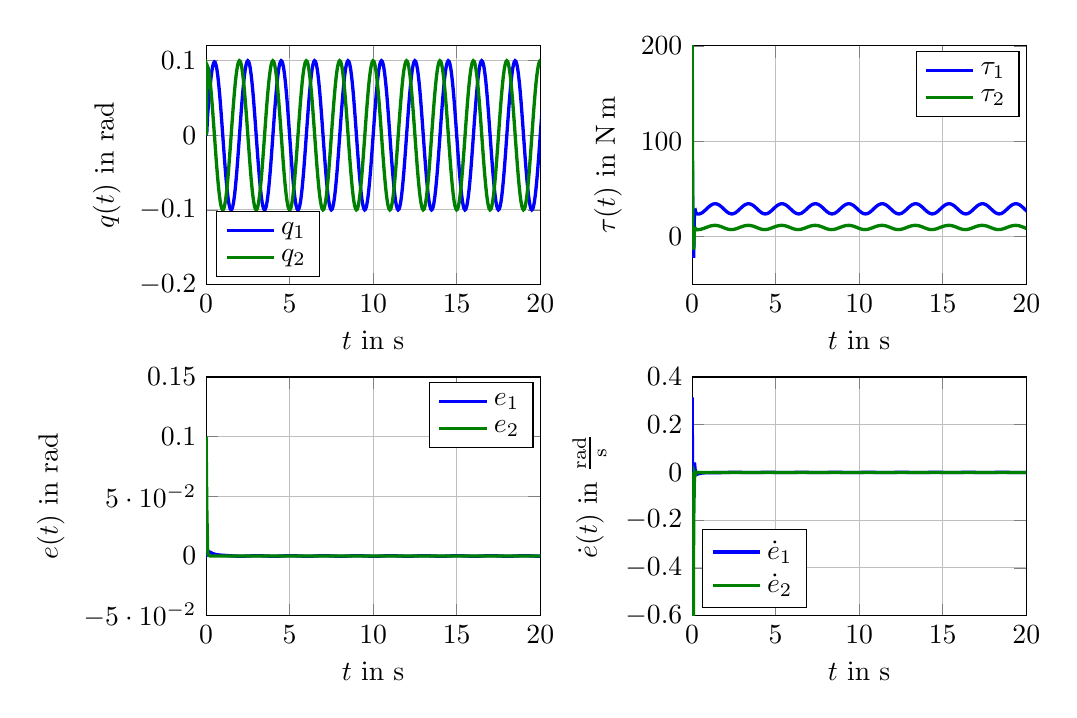
\begin{tikzpicture}

\begin{axis}[%
width=0.35\textwidth,
height=0.25\textwidth,
scale only axis,
xmin=0,
xmax=20,
xlabel={$t$ in $\mathrm{s}$},
xmajorgrids,
ymin=-0.2,
ymax=0.12,
ylabel={$q(t)$ in $\mathrm{rad}$},
ymajorgrids,
name=plot1,
legend style={at={(0.03,0.03)},anchor=south west,draw=black,fill=white,legend cell align=left}
]
\addplot [
color=blue,
solid,
line width=1.2pt
]
table[row sep=crcr]{
0 0\\
0.0435723513550657 0.00432899350231908\\
0.0935723513550658 0.0274004853661707\\
0.143572351355066 0.0412789831145179\\
0.193572351355066 0.0536976195473785\\
0.243572351355066 0.0661155719649353\\
0.293572351355066 0.0769685132168032\\
0.343572351355066 0.0857845589604632\\
0.393572351355066 0.0923867559716492\\
0.443572351355066 0.0966180108750729\\
0.493572351355066 0.0983834204262649\\
0.543572351355066 0.097651769508841\\
0.593572351355066 0.0944512932218814\\
0.643572351355066 0.0888694993928927\\
0.693572351355066 0.0810514439878954\\
0.743572351355066 0.0711962433908491\\
0.793572351355066 0.0595522711799117\\
0.843572351355066 0.0464111407996759\\
0.893572351355066 0.0321006131998071\\
0.943572351355066 0.0169766126348648\\
0.993572351355067 0.00141454897050705\\
1.04357235135506 -0.0141998411792065\\
1.09357235135506 -0.0294799114633308\\
1.14357235135505 -0.0440475522869543\\
1.19357235135505 -0.0575424372905624\\
1.24357235135504 -0.0696308443743869\\
1.29357235135503 -0.0800138349218712\\
1.34357235135503 -0.0884345891073232\\
1.39357235135502 -0.0946847145271886\\
1.44357235135502 -0.0986093696927142\\
1.49357235135501 -0.100111072759448\\
1.54357235135501 -0.0991520985850803\\
1.593572351355 -0.0957554028891489\\
1.643572351355 -0.0900040498186083\\
1.69357235135499 -0.0820391573635999\\
1.74357235135498 -0.0720564125658288\\
1.79357235135498 -0.0603012441601745\\
1.84357235135497 -0.0470627732112735\\
1.89357235135497 -0.03266669169913\\
1.94357235135496 -0.0174672443448138\\
1.99357235135496 -0.0018385099084112\\
2.04357235135495 0.013834805479401\\
2.09357235135495 0.029166838828791\\
2.14357235135494 0.0437800738712218\\
2.19357235135494 0.05731464535373\\
2.24357235135493 0.0694372153492909\\
2.29357235135492 0.0798492019334752\\
2.34357235135492 0.0882941551017915\\
2.39357235135491 0.0945640947605936\\
2.44357235135491 0.0985046507835059\\
2.4935723513549 0.100018875005529\\
2.5435723513549 0.0990696288741785\\
2.59357235135489 0.0956804872713722\\
2.64357235135489 0.0899351375302386\\
2.69357235135488 0.0819752915509206\\
2.74357235135487 0.0719971668283413\\
2.79357235135487 0.0602466279305144\\
2.84357235135486 0.0470131125202827\\
2.89357235135486 0.032622494681437\\
2.94357235135485 0.0174290626453866\\
2.99357235135485 0.00180680778752789\\
3.04357235135484 -0.0138597631166867\\
3.09357235135484 -0.0291850699487942\\
3.14357235135483 -0.0437919274739875\\
3.19357235135482 -0.0573208106758416\\
3.24357235135482 -0.0694386921363723\\
3.29357235135481 -0.0798472354456246\\
3.34357235135481 -0.0882901428122959\\
3.3935723513548 -0.0945594743636576\\
3.4435723513548 -0.0985007808887733\\
3.49357235135479 -0.100016920588334\\
3.54357235135479 -0.0990704630858218\\
3.59357235135478 -0.0956846196152789\\
3.64357235135478 -0.0899426758127276\\
3.69357235135477 -0.0819859416623739\\
3.74357235135476 -0.0720102706325989\\
3.79357235135476 -0.0602612357226507\\
3.84357235135475 -0.0470280830513293\\
3.89357235135475 -0.0326366130019756\\
3.94357235135474 -0.0174411642670147\\
3.99357235135474 -0.0018158970694308\\
4.04357235135475 0.0138544118382747\\
4.09357235135477 0.0291838382403013\\
4.14357235135478 0.0437948127854798\\
4.1935723513548 0.0573274241961538\\
4.24357235135482 0.0694482946380575\\
4.29357235135483 0.0798588075821118\\
4.34357235135485 0.088302483015781\\
4.39357235135487 0.0945713148223287\\
4.44357235135488 0.098510910307302\\
4.4935723513549 0.10002430173346\\
4.54357235135492 0.0990743335740002\\
4.59357235135493 0.095684565989587\\
4.64357235135495 0.0899386735462152\\
4.69357235135497 0.0819783570718385\\
4.74357235135498 0.071999824459389\\
4.793572351355 0.0602489319501677\\
4.84357235135502 0.0470151099865019\\
4.89357235135503 0.0326242263911821\\
4.94357235135505 0.0174305639668675\\
4.99357235135507 0.00180810938203362\\
5.04357235135508 -0.0138586346687685\\
5.0935723513551 -0.0291840916050857\\
5.14357235135512 -0.0437910792593511\\
5.19357235135513 -0.057320075274177\\
5.24357235135515 -0.0694380545366883\\
5.29357235135517 -0.0798466826351833\\
5.34357235135518 -0.088289663510583\\
5.3935723513552 -0.0945590587917532\\
5.44357235135522 -0.0985004205694184\\
5.49357235135524 -0.100016608172611\\
5.54357235135525 -0.0990701922029093\\
5.59357235135527 -0.0956843847422047\\
5.64357235135529 -0.089942472161467\\
5.6935723513553 -0.0819857650819783\\
5.74357235135532 -0.0720101175243583\\
5.79357235135534 -0.0602611029665544\\
5.84357235135535 -0.0470279679423221\\
5.89357235135537 -0.0326365131947074\\
5.94357235135539 -0.017441077727952\\
5.9935723513554 -0.00181582203535077\\
6.04357235135542 0.0138544768962567\\
6.09357235135544 0.0291838946479089\\
6.14357235135545 0.0437948616922983\\
6.19357235135547 0.0573274665990497\\
6.24357235135549 0.0694483314014774\\
6.2935723513555 0.0798588394556778\\
6.34357235135552 0.0883025106495432\\
6.39357235135554 0.094571338779988\\
6.44357235135555 0.0985109310776749\\
6.49357235135557 0.100024319740419\\
6.54357235135559 0.0990743491850942\\
6.5935723513556 0.0956845795235183\\
6.64357235135562 0.0899386852793227\\
6.69357235135564 0.081978367243722\\
6.74357235135565 0.0719998332777879\\
6.79357235135567 0.0602489395951923\\
6.84357235135569 0.047015116614304\\
6.8935723513557 0.0326242321371386\\
6.94357235135572 0.0174305689483421\\
6.99357235135574 0.00180811370077149\\
7.04357235135575 -0.0138586309245632\\
7.09357235135577 -0.0291840883589487\\
7.14357235135579 -0.043791076444996\\
7.1935723513558 -0.057320072834141\\
7.24357235135582 -0.0694380524211576\\
7.29357235135584 -0.0798466808009755\\
7.34357235135585 -0.088289661920264\\
7.39357235135587 -0.094559057412872\\
7.44357235135589 -0.0985004193738443\\
7.4935723513559 -0.100016607135958\\
7.54357235135592 -0.0990701913040375\\
7.59357235135594 -0.0956843839627886\\
7.64357235135595 -0.0899424714856204\\
7.69357235135597 -0.0819857644959298\\
7.74357235135599 -0.0720101170161696\\
7.793572351356 -0.0602611025258763\\
7.84357235135602 -0.0470279675601829\\
7.89357235135604 -0.0326365128633293\\
7.94357235135605 -0.0174410774405922\\
7.99357235135607 -0.00181582178616359\\
8.04357235135605 0.0138544771123387\\
8.09357235135602 0.0291838948352785\\
8.14357235135599 0.0437948618547649\\
8.19357235135596 0.0573274667399171\\
8.24357235135594 0.0694483315236112\\
8.29357235135591 0.0798588395615639\\
8.34357235135588 0.088302510741338\\
8.39357235135585 0.0945713388595625\\
8.44357235135583 0.0985109311466526\\
8.4935723513558 0.100024319800208\\
8.54357235135577 0.0990743492369187\\
8.59357235135574 0.0956845795684381\\
8.64357235135572 0.0899386853182584\\
8.69357235135569 0.0819783672774722\\
8.74357235135566 0.0719998333070452\\
8.79357235135563 0.0602489396205572\\
8.8435723513556 0.0470151166362973\\
8.89357235135558 0.0326242321562113\\
8.94357235135555 0.0174305689648846\\
8.99357235135552 0.00180811371512181\\
9.04357235135549 -0.0138586309121129\\
9.09357235135547 -0.0291840883481461\\
9.14357235135544 -0.0437910764356233\\
9.19357235135541 -0.0573200728260103\\
9.24357235135538 -0.069438052414107\\
9.29357235135535 -0.0798466807948657\\
9.34357235135533 -0.0882896619149748\\
9.3935723513553 -0.0945590574083\\
9.44357235135527 -0.0985004193699001\\
9.49357235135524 -0.100016607132565\\
9.54357235135522 -0.0990701913011278\\
9.59357235135519 -0.0956843839603044\\
9.64357235135516 -0.0899424714835109\\
9.69357235135513 -0.0819857644941498\\
9.74357235135511 -0.0720101170146791\\
9.79357235135508 -0.0602611025246392\\
9.84357235135505 -0.0470279675591665\\
9.89357235135502 -0.0326365128625038\\
9.94357235135499 -0.0174410774399298\\
9.99357235135497 -0.00181582178563861\\
10.0435723513549 0.013854477112751\\
10.0935723513549 0.029183894835602\\
10.1435723513549 0.0437948618550211\\
10.1935723513549 0.0573274667401253\\
10.2435723513548 0.0694483315237885\\
10.2935723513548 0.0798588395617252\\
10.3435723513548 0.088302510741496\\
10.3935723513547 0.0945713388597279\\
10.4435723513547 0.0985109311468338\\
10.4935723513547 0.100024319800412\\
10.5435723513547 0.0990743492371488\\
10.5935723513546 0.0956845795686974\\
10.6435723513546 0.0899386853185476\\
10.6935723513546 0.0819783672777902\\
10.7435723513546 0.0719998333073897\\
10.7935723513545 0.0602489396209243\\
10.8435723513545 0.0470151166366819\\
10.8935723513545 0.0326242321566074\\
10.9435723513544 0.0174305689652856\\
10.9935723513544 0.00180811371552037\\
11.0435723513544 -0.0138586309117244\\
11.0935723513544 -0.0291840883477752\\
11.1435723513543 -0.0437910764352773\\
11.1935723513543 -0.0573200728256963\\
11.2435723513543 -0.0694380524138316\\
11.2935723513542 -0.0798466807946345\\
11.3435723513542 -0.0882896619147924\\
11.3935723513542 -0.0945590574081702\\
11.4435723513542 -0.0985004193698254\\
11.4935723513541 -0.100016607132546\\
11.5435723513541 -0.0990701913011656\\
11.5935723513541 -0.095684383960397\\
11.6435723513541 -0.0899424714836555\\
11.693572351354 -0.0819857644943426\\
11.743572351354 -0.0720101170149151\\
11.793572351354 -0.0602611025249123\\
11.8435723513539 -0.0470279675594697\\
11.8935723513539 -0.0326365128628294\\
11.9435723513539 -0.0174410774402696\\
11.9935723513539 -0.00181582178598415\\
12.0435723513538 0.0138544771124083\\
12.0935723513538 0.0291838948352708\\
12.1435723513538 0.0437948618547097\\
12.1935723513537 0.0573274667398413\\
12.2435723513537 0.0694483315235391\\
12.2935723513537 0.0798588395615165\\
12.3435723513537 0.0883025107413332\\
12.3935723513536 0.0945713388596151\\
12.4435723513536 0.0985109311467738\\
12.4935723513536 0.100024319800406\\
12.5435723513536 0.0990743492371977\\
12.5935723513535 0.0956845795687997\\
12.6435723513535 0.0899386853187006\\
12.6935723513535 0.0819783672779904\\
12.7435723513534 0.071999833307632\\
12.7935723513534 0.0602489396212028\\
12.8435723513534 0.0470151166369897\\
12.8935723513534 0.032624232156937\\
12.9435723513533 0.0174305689656288\\
12.9935723513533 0.00180811371586885\\
13.0435723513533 -0.0138586309113792\\
13.0935723513532 -0.0291840883474419\\
13.1435723513532 -0.043791076434964\\
13.1935723513532 -0.0573200728254107\\
13.2435723513532 -0.0694380524135808\\
13.2935723513531 -0.0798466807944245\\
13.3435723513531 -0.0882896619146286\\
13.3935723513531 -0.0945590574080564\\
13.4435723513531 -0.0985004193697645\\
13.493572351353 -0.10001660713254\\
13.543572351353 -0.0990701913012137\\
13.593572351353 -0.0956843839604985\\
13.6435723513529 -0.0899424714838079\\
13.6935723513529 -0.0819857644945421\\
13.7435723513529 -0.0720101170151568\\
13.7935723513529 -0.0602611025251902\\
13.8435723513528 -0.0470279675597771\\
13.8935723513528 -0.0326365128631586\\
13.9435723513528 -0.0174410774406126\\
13.9935723513528 -0.00181582178633244\\
14.0435723513527 0.0138544771120633\\
14.0935723513527 0.0291838948349376\\
14.1435723513527 0.0437948618543964\\
14.1935723513526 0.0573274667395558\\
14.2435723513526 0.0694483315232883\\
14.2935723513526 0.0798588395613066\\
14.3435723513526 0.0883025107411695\\
14.3935723513525 0.0945713388595015\\
14.4435723513525 0.0985109311467132\\
14.4935723513525 0.1000243198004\\
14.5435723513524 0.099074349237246\\
14.5935723513524 0.0956845795689013\\
14.6435723513524 0.0899386853188531\\
14.6935723513524 0.08197836727819\\
14.7435723513523 0.0719998333078737\\
14.7935723513523 0.0602489396214808\\
14.8435723513523 0.0470151166372971\\
14.8935723513523 0.0326242321572662\\
14.9435723513522 0.0174305689659718\\
14.9935723513522 0.00180811371621705\\
15.0435723513522 -0.0138586309110343\\
15.0935723513521 -0.0291840883471087\\
15.1435723513521 -0.0437910764346508\\
15.1935723513521 -0.0573200728251253\\
15.2435723513521 -0.0694380524133301\\
15.293572351352 -0.0798466807942147\\
15.343572351352 -0.0882896619144649\\
15.393572351352 -0.0945590574079428\\
15.4435723513519 -0.0985004193697039\\
15.4935723513519 -0.100016607132534\\
15.5435723513519 -0.099070191301262\\
15.5935723513519 -0.0956843839606001\\
15.6435723513518 -0.0899424714839604\\
15.6935723513518 -0.0819857644947418\\
15.7435723513518 -0.0720101170153987\\
15.7935723513518 -0.0602611025254684\\
15.8435723513517 -0.0470279675600847\\
15.8935723513517 -0.032636512863488\\
15.9435723513517 -0.0174410774409558\\
15.9935723513516 -0.00181582178668087\\
16.0435723513517 0.0138544771117192\\
16.0935723513518 0.0291838948346086\\
16.1435723513518 0.0437948618540913\\
16.1935723513519 0.0573274667392808\\
16.2435723513519 0.0694483315230478\\
16.293572351352 0.0798588395611025\\
16.3435723513521 0.0883025107410016\\
16.3935723513521 0.0945713388593678\\
16.4435723513522 0.0985109311466102\\
16.4935723513522 0.100024319800323\\
16.5435723513523 0.0990743492371887\\
16.5935723513524 0.0956845795688575\\
16.6435723513524 0.0899386853188164\\
16.6935723513525 0.0819783672781541\\
16.7435723513525 0.071999833307833\\
16.7935723513526 0.0602489396214305\\
16.8435723513527 0.0470151166372335\\
16.8935723513527 0.0326242321571873\\
16.9435723513528 0.0174305689658768\\
16.9935723513529 0.00180811371610725\\
17.0435723513529 -0.0138586309111562\\
17.093572351353 -0.0291840883472383\\
17.143572351353 -0.0437910764347821\\
17.1935723513531 -0.0573200728252512\\
17.2435723513532 -0.0694380524134422\\
17.2935723513532 -0.0798466807943042\\
17.3435723513533 -0.0882896619145224\\
17.3935723513533 -0.0945590574079592\\
17.4435723513534 -0.0985004193696704\\
17.4935723513535 -0.100016607132442\\
17.5435723513535 -0.0990701913011065\\
17.5935723513536 -0.0956843839603755\\
17.6435723513536 -0.0899424714836638\\
17.6935723513537 -0.0819857644943725\\
17.7435723513538 -0.0720101170149587\\
17.7935723513538 -0.0602611025249622\\
17.8435723513539 -0.0470279675595194\\
17.893572351354 -0.0326365128628736\\
17.943572351354 -0.0174410774403044\\
17.9935723513541 -0.00181582178600701\\
18.0435723513541 0.0138544771123981\\
18.0935723513542 0.0291838948352723\\
18.1435723513543 0.0437948618547202\\
18.1935723513543 0.0573274667398569\\
18.2435723513544 0.0694483315235542\\
18.2935723513544 0.0798588395615248\\
18.3435723513545 0.0883025107413277\\
18.3935723513546 0.094571338859588\\
18.4435723513546 0.0985109311467176\\
18.4935723513547 0.100024319800314\\
18.5435723513547 0.0990743492370624\\
18.5935723513548 0.0956845795686162\\
18.6435723513549 0.0899386853184652\\
18.6935723513549 0.081978367277701\\
18.743572351355 0.0719998333072885\\
18.7935723513551 0.0602489396208076\\
18.8435723513551 0.0470151166365471\\
18.8935723513552 0.0326242321564539\\
18.9435723513552 0.0174305689651142\\
18.9935723513553 0.00180811371533384\\
19.0435723513554 -0.0138586309119216\\
19.0935723513554 -0.029184088347977\\
19.1435723513555 -0.0437910764354762\\
19.1935723513555 -0.0573200728258837\\
19.2435723513556 -0.0694380524139977\\
19.2935723513557 -0.0798466807947691\\
19.3435723513557 -0.0882896619148855\\
19.3935723513558 -0.0945590574082115\\
19.4435723513558 -0.0985004193698057\\
19.4935723513559 -0.100016607132458\\
19.543572351356 -0.0990701913010012\\
19.593572351356 -0.0956843839601523\\
19.6435723513561 -0.0899424714833283\\
19.6935723513562 -0.081985764493933\\
19.7435723513562 -0.072010117014426\\
19.7935723513563 -0.0602611025243495\\
19.8435723513563 -0.0470279675588418\\
19.8935723513564 -0.0326365128621478\\
19.9435723513565 -0.0174410774395482\\
19.9935723513565 -0.00181582178523916\\
20.0435723513566 0.0138544771131587\\
20.0935723513566 0.0291838948360069\\
20.1435723513567 0.0437948618554108\\
20.1935723513568 0.0573274667404864\\
20.2435723513568 0.0694483315241071\\
20.2935723513569 0.0798588395619875\\
20.3435723513569 0.0883025107416888\\
20.393572351357 0.0945713388598385\\
20.4435723513571 0.0985109311468514\\
20.4935723513571 0.100024319800328\\
20.5435723513572 0.0990743492369559\\
20.5935723513573 0.095684579568392\\
20.6435723513573 0.0899386853181288\\
20.6935723513574 0.0819783672772607\\
20.7435723513574 0.0719998333067553\\
20.7935723513575 0.0602489396201944\\
20.8435723513576 0.0470151166358692\\
20.8935723513576 0.0326242321557278\\
20.9435723513577 0.0174305689643579\\
20.9935723513577 0.00180811371456594\\
21.0435723513578 -0.0138586309126822\\
21.0935723513579 -0.0291840883487116\\
21.1435723513579 -0.0437910764361668\\
21.193572351358 -0.0573200728265131\\
21.243572351358 -0.0694380524145506\\
21.2935723513581 -0.0798466807952318\\
21.3435723513582 -0.0882896619152465\\
21.3935723513582 -0.0945590574084621\\
21.4435723513583 -0.0985004193699397\\
21.4935723513584 -0.100016607132472\\
21.5435723513584 -0.0990701913008949\\
21.5935723513585 -0.0956843839599284\\
21.6435723513585 -0.0899424714829921\\
21.6935723513586 -0.0819857644934929\\
21.7435723513587 -0.0720101170138929\\
21.7935723513587 -0.0602611025237364\\
21.8435723513588 -0.0470279675581639\\
21.8935723513588 -0.0326365128614216\\
21.9435723513589 -0.0174410774387918\\
21.993572351359 -0.00181582178447107\\
22.043572351359 0.0138544771139195\\
22.0935723513591 0.0291838948367417\\
22.1435723513591 0.0437948618561015\\
22.1935723513592 0.057327466741116\\
22.2435723513593 0.0694483315246601\\
22.2935723513593 0.0798588395624502\\
22.3435723513594 0.0883025107420498\\
22.3935723513595 0.0945713388600891\\
22.4435723513595 0.0985109311469854\\
22.4935723513596 0.100024319800341\\
22.5435723513596 0.0990743492368494\\
22.5935723513597 0.0956845795681678\\
22.6435723513598 0.0899386853177925\\
22.6935723513598 0.0819783672768205\\
22.7435723513599 0.071999833306222\\
22.7935723513599 0.0602489396195812\\
22.84357235136 0.0470151166351912\\
22.8935723513601 0.0326242321550017\\
22.9435723513601 0.0174305689636016\\
22.9935723513602 0.001808113713798\\
23.0435723513602 -0.0138586309134429\\
23.0935723513603 -0.0291840883494463\\
23.1435723513604 -0.0437910764368573\\
23.1935723513604 -0.0573200728271426\\
23.2435723513605 -0.0694380524151035\\
23.2935723513606 -0.0798466807956945\\
23.3435723513606 -0.0882896619156076\\
23.3935723513607 -0.0945590574087127\\
23.4435723513607 -0.0985004193700736\\
23.4935723513608 -0.100016607132486\\
23.5435723513609 -0.0990701913007886\\
23.5935723513609 -0.0956843839597044\\
23.643572351361 -0.089942471482656\\
23.693572351361 -0.0819857644930529\\
23.7435723513611 -0.0720101170133597\\
23.7935723513612 -0.0602611025231233\\
23.8435723513612 -0.0470279675574859\\
23.8935723513613 -0.0326365128606955\\
23.9435723513613 -0.0174410774380354\\
23.9935723513614 -0.00181582178370301\\
24.0435723513615 0.0138544771146803\\
24.0935723513615 0.0291838948374765\\
24.1435723513616 0.0437948618567922\\
24.1935723513617 0.0573274667417455\\
24.2435723513617 0.0694483315252131\\
24.2935723513618 0.079858839562913\\
24.3435723513618 0.0883025107424109\\
24.3935723513619 0.0945713388603396\\
24.443572351362 0.0985109311471191\\
24.493572351362 0.100024319800355\\
24.5435723513621 0.0990743492367428\\
24.5935723513621 0.0956845795679435\\
24.6435723513622 0.0899386853174561\\
24.6935723513623 0.0819783672763802\\
24.7435723513623 0.0719998333056887\\
24.7935723513624 0.0602489396189681\\
24.8435723513624 0.0470151166345132\\
24.8935723513625 0.0326242321542757\\
24.9435723513626 0.0174305689628453\\
24.9935723513626 0.00180811371303012\\
25.0435723513627 -0.0138586309142035\\
25.0935723513628 -0.0291840883501808\\
25.1435723513628 -0.0437910764375478\\
25.1935723513629 -0.057320072827772\\
25.2435723513629 -0.0694380524156563\\
25.293572351363 -0.0798466807961571\\
25.3435723513631 -0.0882896619159687\\
25.3935723513631 -0.0945590574089633\\
25.4435723513632 -0.0985004193702076\\
25.4935723513632 -0.1000166071325\\
25.5435723513633 -0.0990701913006822\\
25.5935723513634 -0.0956843839594803\\
25.6435723513634 -0.0899424714823197\\
25.6935723513635 -0.0819857644926127\\
25.7435723513635 -0.0720101170128265\\
25.7935723513636 -0.0602611025225101\\
25.8435723513637 -0.0470279675568079\\
25.8935723513637 -0.0326365128599694\\
25.9435723513638 -0.017441077437279\\
25.9935723513639 -0.00181582178293494\\
26.0435723513639 0.0138544771154412\\
26.093572351364 0.0291838948382114\\
26.143572351364 0.0437948618574829\\
26.1935723513641 0.0573274667423751\\
26.2435723513642 0.069448331525766\\
26.2935723513642 0.0798588395633756\\
26.3435723513643 0.0883025107427719\\
26.3935723513643 0.0945713388605901\\
26.4435723513644 0.0985109311472529\\
26.4935723513645 0.100024319800369\\
26.5435723513645 0.0990743492366363\\
26.5935723513646 0.0956845795677193\\
26.6435723513646 0.0899386853171197\\
26.6935723513647 0.0819783672759399\\
26.7435723513648 0.0719998333051553\\
26.7935723513648 0.0602489396183548\\
26.8435723513649 0.0470151166338352\\
26.893572351365 0.0326242321535496\\
26.943572351365 0.017430568962089\\
26.9935723513651 0.00180811371226217\\
27.0435723513651 -0.0138586309149641\\
27.0935723513652 -0.0291840883509155\\
27.1435723513653 -0.0437910764382384\\
27.1935723513653 -0.0573200728284015\\
27.2435723513654 -0.0694380524162092\\
27.2935723513654 -0.0798466807966198\\
27.3435723513655 -0.0882896619163298\\
27.3935723513656 -0.0945590574092139\\
27.4435723513656 -0.0985004193703415\\
27.4935723513657 -0.100016607132514\\
27.5435723513657 -0.0990701913005759\\
27.5935723513658 -0.0956843839592563\\
27.6435723513659 -0.0899424714819835\\
27.6935723513659 -0.0819857644921726\\
27.743572351366 -0.0720101170122933\\
27.7935723513661 -0.0602611025218969\\
27.8435723513661 -0.0470279675561299\\
27.8935723513662 -0.0326365128592431\\
27.9435723513662 -0.0174410774365225\\
27.9935723513663 -0.00181582178216681\\
28.0435723513664 0.013854477116202\\
28.0935723513664 0.0291838948389462\\
28.1435723513665 0.0437948618581737\\
28.1935723513665 0.0573274667430048\\
28.2435723513666 0.0694483315263191\\
28.2935723513667 0.0798588395638385\\
28.3435723513667 0.0883025107431331\\
28.3935723513668 0.0945713388608408\\
28.4435723513668 0.0985109311473869\\
28.4935723513669 0.100024319800383\\
28.543572351367 0.0990743492365299\\
28.593572351367 0.0956845795674952\\
28.6435723513671 0.0899386853167834\\
28.6935723513672 0.0819783672754998\\
28.7435723513672 0.0719998333046222\\
28.7935723513673 0.0602489396177417\\
28.8435723513673 0.0470151166331573\\
28.8935723513674 0.0326242321528235\\
28.9435723513675 0.0174305689613327\\
28.9935723513675 0.00180811371149428\\
29.0435723513676 -0.0138586309157247\\
29.0935723513676 -0.0291840883516501\\
29.1435723513677 -0.0437910764389289\\
29.1935723513678 -0.0573200728290308\\
29.2435723513678 -0.069438052416762\\
29.2935723513679 -0.0798466807970825\\
29.3435723513679 -0.0882896619166908\\
29.393572351368 -0.0945590574094645\\
29.4435723513681 -0.0985004193704755\\
29.4935723513681 -0.100016607132528\\
29.5435723513682 -0.0990701913004696\\
29.5935723513683 -0.0956843839590323\\
29.6435723513683 -0.0899424714816473\\
29.6935723513684 -0.0819857644917325\\
29.7435723513684 -0.0720101170117601\\
29.7935723513685 -0.0602611025212838\\
29.8435723513686 -0.0470279675554519\\
29.8935723513686 -0.032636512858517\\
29.9435723513687 -0.0174410774357661\\
29.9935723513687 -0.00181582178139874\\
30.0435723513688 0.0138544771169628\\
30.0935723513689 0.029183894839681\\
30.1435723513689 0.0437948618588644\\
30.193572351369 0.0573274667436344\\
30.243572351369 0.069448331526872\\
30.2935723513691 0.0798588395643012\\
30.3435723513692 0.0883025107434941\\
30.3935723513692 0.0945713388610912\\
30.4435723513693 0.0985109311475206\\
30.4935723513694 0.100024319800397\\
30.5435723513694 0.0990743492364233\\
30.5935723513695 0.0956845795672709\\
30.6435723513695 0.0899386853164469\\
30.6935723513696 0.0819783672750594\\
30.7435723513697 0.0719998333040888\\
30.7935723513697 0.0602489396171284\\
30.8435723513698 0.0470151166324793\\
30.8935723513698 0.0326242321520974\\
30.9435723513699 0.0174305689605764\\
30.99357235137 0.00180811371072636\\
31.04357235137 -0.0138586309164854\\
31.0935723513701 -0.0291840883523847\\
31.1435723513701 -0.0437910764396194\\
31.1935723513702 -0.0573200728296603\\
31.2435723513703 -0.0694380524173149\\
31.2935723513703 -0.0798466807975452\\
31.3435723513704 -0.088289661917052\\
31.3935723513705 -0.094559057409715\\
31.4435723513705 -0.0985004193706094\\
31.4935723513706 -0.100016607132542\\
31.5435723513706 -0.0990701913003633\\
31.5935723513707 -0.0956843839588082\\
31.6435723513708 -0.0899424714813111\\
31.6935723513708 -0.0819857644912924\\
31.7435723513709 -0.0720101170112269\\
31.7935723513709 -0.0602611025206707\\
31.843572351371 -0.0470279675547739\\
31.8935723513711 -0.0326365128577909\\
31.9435723513711 -0.0174410774350097\\
31.9935723513712 -0.00181582178063066\\
32.0435723513711 0.0138544771177218\\
32.093572351371 0.0291838948404073\\
32.1435723513709 0.043794861859539\\
32.1935723513707 0.0573274667442429\\
32.2435723513706 0.0694483315274047\\
32.2935723513705 0.0798588395647526\\
32.3435723513704 0.0883025107438636\\
32.3935723513703 0.0945713388613819\\
32.4435723513702 0.0985109311477391\\
32.49357235137 0.100024319800552\\
32.5435723513699 0.0990743492365279\\
32.5935723513698 0.0956845795673372\\
32.6435723513697 0.0899386853164884\\
32.6935723513696 0.0819783672750895\\
32.7435723513695 0.0719998333041199\\
32.7935723513693 0.0602489396171714\\
32.8435723513692 0.0470151166325426\\
32.8935723513691 0.032624232152187\\
32.943572351369 0.0174305689606951\\
32.9935723513689 0.0018081137108737\\
33.0435723513688 -0.0138586309163132\\
33.0935723513686 -0.0291840883521947\\
33.1435723513685 -0.0437910764394218\\
33.1935723513684 -0.057320072829468\\
33.2435723513683 -0.0694380524171428\\
33.2935723513682 -0.0798466807974098\\
33.3435723513681 -0.0882896619169709\\
33.3935723513679 -0.094559057409706\\
33.4435723513678 -0.0985004193706891\\
33.4935723513677 -0.100016607132725\\
33.5435723513676 -0.0990701913006644\\
33.5935723513675 -0.0956843839592366\\
33.6435723513674 -0.089942471481873\\
33.6935723513672 -0.0819857644919898\\
33.7435723513671 -0.072010117012057\\
33.793572351367 -0.0602611025216256\\
33.8435723513669 -0.0470279675558407\\
33.8935723513668 -0.0326365128589516\\
33.9435723513667 -0.0174410774362414\\
33.9935723513665 -0.00181582178190622\\
34.0435723513664 0.0138544771164353\\
34.0935723513663 0.0291838948391489\\
34.1435723513662 0.0437948618583458\\
34.1935723513661 0.0573274667431498\\
34.243572351366 0.0694483315264433\\
34.2935723513658 0.079858839563951\\
34.3435723513657 0.0883025107432451\\
34.3935723513656 0.0945713388609649\\
34.4435723513655 0.0985109311475366\\
34.4935723513654 0.100024319800572\\
34.5435723513653 0.0990743492367706\\
34.5935723513651 0.0956845795677991\\
34.643572351365 0.0899386853171598\\
34.6935723513649 0.081978367275955\\
34.7435723513648 0.0719998333051594\\
34.7935723513647 0.0602489396183602\\
34.8435723513646 0.0470151166338524\\
34.8935723513644 0.0326242321535864\\
34.9435723513643 0.0174305689621501\\
34.9935723513642 0.0018081137123492\\
35.0435723513641 -0.013858630914853\\
35.093572351364 -0.0291840883507855\\
35.1435723513639 -0.0437910764380977\\
35.1935723513637 -0.0573200728282613\\
35.2435723513636 -0.069438052416083\\
35.2935723513635 -0.0798466807965228\\
35.3435723513634 -0.0882896619162783\\
35.3935723513633 -0.0945590574092245\\
35.4435723513632 -0.0985004193704306\\
35.493572351363 -0.100016607132696\\
35.5435723513629 -0.0990701913008649\\
35.5935723513628 -0.0956843839596618\\
35.6435723513627 -0.0899424714825124\\
35.6935723513626 -0.0819857644928275\\
35.7435723513625 -0.0720101170130725\\
35.7935723513624 -0.0602611025227937\\
35.8435723513622 -0.0470279675571327\\
35.8935723513621 -0.0326365128603355\\
35.943572351362 -0.0174410774376832\\
35.9935723513619 -0.00181582178337036\\
36.0435723513618 0.013854477114985\\
36.0935723513617 0.0291838948377481\\
36.1435723513615 0.043794861857029\\
36.1935723513614 0.0573274667419494\\
36.2435723513613 0.0694483315253891\\
36.2935723513612 0.0798588395630689\\
36.3435723513611 0.0883025107425568\\
36.393572351361 0.0945713388604873\\
36.4435723513608 0.0985109311472815\\
36.4935723513607 0.100024319800545\\
36.5435723513606 0.0990743492369738\\
36.5935723513605 0.0956845795682268\\
36.6435723513604 0.0899386853178014\\
36.6935723513603 0.0819783672767948\\
36.7435723513601 0.0719998333061766\\
36.79357235136 0.0602489396195298\\
36.8435723513599 0.0470151166351455\\
36.8935723513598 0.0326242321549711\\
36.9435723513597 0.0174305689635925\\
36.9935723513596 0.00180811371381373\\
37.0435723513594 -0.0138586309134024\\
37.0935723513593 -0.0291840883493845\\
37.1435723513592 -0.0437910764367808\\
37.1935723513591 -0.0573200728270609\\
37.243572351359 -0.0694380524150286\\
37.2935723513589 -0.0798466807956404\\
37.3435723513587 -0.0882896619155897\\
37.3935723513586 -0.0945590574087467\\
37.4435723513585 -0.0985004193701753\\
37.4935723513584 -0.10001660713267\\
37.5435723513583 -0.0990701913010677\\
37.5935723513582 -0.0956843839600891\\
37.643572351358 -0.0899424714831537\\
37.6935723513579 -0.0819857644936669\\
37.7435723513578 -0.0720101170140893\\
37.7935723513577 -0.0602611025239631\\
37.8435723513576 -0.0470279675584257\\
37.8935723513575 -0.0326365128617204\\
37.9435723513573 -0.0174410774391258\\
37.9935723513572 -0.00181582178483517\\
38.0435723513571 0.013854477113534\\
38.093572351357 0.0291838948363467\\
38.1435723513569 0.0437948618557118\\
38.1935723513568 0.0573274667407487\\
38.2435723513566 0.0694483315243345\\
38.2935723513565 0.0798588395621864\\
38.3435723513564 0.0883025107418682\\
38.3935723513563 0.0945713388600095\\
38.4435723513562 0.0985109311470263\\
38.4935723513561 0.100024319800519\\
38.5435723513559 0.099074349237177\\
38.5935723513558 0.0956845795686544\\
38.6435723513557 0.0899386853184428\\
38.6935723513556 0.0819783672776343\\
38.7435723513555 0.0719998333071935\\
38.7935723513554 0.060248939620699\\
38.8435723513552 0.0470151166364383\\
38.8935723513551 0.0326242321563557\\
38.943572351355 0.0174305689650347\\
38.9935723513549 0.00180811371527811\\
39.0435723513548 -0.0138586309119519\\
39.0935723513547 -0.0291840883479836\\
39.1435723513545 -0.043791076435464\\
39.1935723513544 -0.0573200728258605\\
39.2435723513543 -0.0694380524139743\\
39.2935723513542 -0.0798466807947581\\
39.3435723513541 -0.0882896619149011\\
39.393572351354 -0.0945590574082688\\
39.4435723513538 -0.0985004193699198\\
39.4935723513537 -0.100016607132643\\
39.5435723513536 -0.0990701913012704\\
39.5935723513535 -0.0956843839605163\\
39.6435723513534 -0.0899424714837947\\
39.6935723513533 -0.0819857644945061\\
39.7435723513531 -0.072010117015106\\
39.793572351353 -0.0602611025251321\\
39.8435723513529 -0.0470279675597185\\
39.8935723513528 -0.032636512863105\\
39.9435723513527 -0.0174410774405683\\
39.9935723513526 -0.00181582178629985\\
40.0435723513524 0.0138544771120832\\
40.0935723513523 0.0291838948349454\\
40.1435723513522 0.0437948618543946\\
40.1935723513521 0.0573274667395481\\
40.243572351352 0.06944833152328\\
40.2935723513519 0.0798588395613039\\
40.3435723513517 0.0883025107411795\\
40.3935723513516 0.0945713388595316\\
40.4435723513515 0.098510931146771\\
40.4935723513514 0.100024319800493\\
40.5435723513513 0.09907434923738\\
40.5935723513512 0.0956845795690819\\
40.643572351351 0.0899386853190843\\
40.6935723513509 0.0819783672784739\\
40.7435723513508 0.0719998333082106\\
40.7935723513507 0.0602489396218685\\
40.8435723513506 0.0470151166377313\\
40.8935723513505 0.0326242321577404\\
40.9435723513503 0.0174305689664771\\
40.9935723513502 0.00180811371674263\\
41.0435723513501 -0.0138586309105013\\
41.09357235135 -0.0291840883465826\\
41.1435723513499 -0.0437910764341471\\
41.1935723513498 -0.0573200728246602\\
41.2435723513496 -0.0694380524129199\\
41.2935723513495 -0.0798466807938758\\
41.3435723513494 -0.0882896619142125\\
41.3935723513493 -0.0945590574077909\\
41.4435723513492 -0.0985004193696643\\
41.4935723513491 -0.100016607132616\\
41.5435723513489 -0.0990701913014732\\
41.5935723513488 -0.0956843839609436\\
41.6435723513487 -0.0899424714844359\\
41.6935723513486 -0.0819857644953455\\
41.7435723513485 -0.0720101170161229\\
41.7935723513484 -0.0602611025263016\\
41.8435723513483 -0.0470279675610115\\
41.8935723513481 -0.0326365128644899\\
41.943572351348 -0.0174410774420109\\
41.9935723513479 -0.00181582178776469\\
42.0435723513478 0.0138544771106322\\
42.0935723513477 0.029183894833544\\
42.1435723513476 0.0437948618530773\\
42.1935723513474 0.0573274667383474\\
42.2435723513473 0.0694483315222254\\
42.2935723513472 0.0798588395604215\\
42.3435723513471 0.0883025107404909\\
42.393572351347 0.0945713388590539\\
42.4435723513469 0.0985109311465159\\
42.4935723513467 0.100024319800466\\
42.5435723513466 0.0990743492375832\\
42.5935723513465 0.0956845795695095\\
42.6435723513464 0.0899386853197258\\
42.6935723513463 0.0819783672793136\\
42.7435723513462 0.0719998333092277\\
42.793572351346 0.0602489396230379\\
42.8435723513459 0.0470151166390244\\
42.8935723513458 0.0326242321591252\\
42.9435723513457 0.0174305689679195\\
42.9935723513456 0.00180811371820717\\
43.0435723513455 -0.0138586309090507\\
43.0935723513453 -0.0291840883451816\\
43.1435723513452 -0.0437910764328302\\
43.1935723513451 -0.0573200728234597\\
43.243572351345 -0.0694380524118656\\
43.2935723513449 -0.0798466807929934\\
43.3435723513448 -0.0882896619135238\\
43.3935723513446 -0.0945590574073129\\
43.4435723513445 -0.0985004193694088\\
43.4935723513444 -0.100016607132589\\
43.5435723513443 -0.0990701913016758\\
43.5935723513442 -0.0956843839613706\\
43.6435723513441 -0.0899424714850769\\
43.6935723513439 -0.0819857644961848\\
43.7435723513438 -0.0720101170171397\\
43.7935723513437 -0.0602611025274709\\
43.8435723513436 -0.0470279675623045\\
43.8935723513435 -0.0326365128658747\\
43.9435723513434 -0.0174410774434534\\
43.9935723513432 -0.00181582178922946\\
44.0435723513431 0.0138544771091813\\
44.093572351343 0.0291838948321427\\
44.1435723513429 0.04379486185176\\
44.1935723513428 0.0573274667371467\\
44.2435723513427 0.0694483315211708\\
44.2935723513425 0.079858839559539\\
44.3435723513424 0.0883025107398023\\
44.3935723513423 0.0945713388585761\\
44.4435723513422 0.0985109311462606\\
44.4935723513421 0.10002431980044\\
44.543572351342 0.0990743492377862\\
44.5935723513418 0.0956845795699371\\
44.6435723513417 0.0899386853203674\\
44.6935723513416 0.0819783672801531\\
44.7435723513415 0.0719998333102446\\
44.7935723513414 0.0602489396242073\\
44.8435723513413 0.0470151166403172\\
44.8935723513411 0.0326242321605098\\
44.943572351341 0.0174305689693618\\
44.9935723513409 0.00180811371967157\\
45.0435723513408 -0.0138586309076001\\
45.0935723513407 -0.0291840883437806\\
45.1435723513406 -0.0437910764315133\\
45.1935723513404 -0.0573200728222594\\
45.2435723513403 -0.0694380524108112\\
45.2935723513402 -0.0798466807921111\\
45.3435723513401 -0.0882896619128352\\
45.39357235134 -0.094559057406835\\
45.4435723513399 -0.0985004193691534\\
45.4935723513397 -0.100016607132563\\
45.5435723513396 -0.0990701913018787\\
45.5935723513395 -0.0956843839617979\\
45.6435723513394 -0.0899424714857182\\
45.6935723513393 -0.0819857644970241\\
45.7435723513392 -0.0720101170181565\\
45.793572351339 -0.0602611025286401\\
45.8435723513389 -0.0470279675635975\\
45.8935723513388 -0.0326365128672595\\
45.9435723513387 -0.017441077444896\\
45.9935723513386 -0.00181582179069425\\
46.0435723513385 0.0138544771077303\\
46.0935723513383 0.0291838948307413\\
46.1435723513382 0.0437948618504427\\
46.1935723513381 0.0573274667359459\\
46.243572351338 0.0694483315201161\\
46.2935723513379 0.0798588395586565\\
46.3435723513378 0.0883025107391136\\
46.3935723513376 0.0945713388580983\\
46.4435723513375 0.0985109311460053\\
46.4935723513374 0.100024319800414\\
46.5435723513373 0.0990743492379893\\
46.5935723513372 0.0956845795703647\\
46.6435723513371 0.0899386853210088\\
46.6935723513369 0.0819783672809927\\
46.7435723513368 0.0719998333112616\\
46.7935723513367 0.0602489396253766\\
46.8435723513366 0.0470151166416102\\
46.8935723513365 0.0326242321618945\\
46.9435723513364 0.0174305689708041\\
46.9935723513362 0.00180811372113605\\
47.0435723513361 -0.0138586309061496\\
47.093572351336 -0.0291840883423797\\
47.1435723513359 -0.0437910764301964\\
47.1935723513358 -0.0573200728210589\\
47.2435723513357 -0.0694380524097569\\
47.2935723513355 -0.0798466807912287\\
47.3435723513354 -0.0882896619121466\\
47.3935723513353 -0.0945590574063572\\
47.4435723513352 -0.0985004193688981\\
47.4935723513351 -0.100016607132536\\
47.543572351335 -0.0990701913020816\\
47.5935723513348 -0.0956843839622252\\
47.6435723513347 -0.0899424714863594\\
47.6935723513346 -0.0819857644978634\\
47.7435723513345 -0.0720101170191734\\
47.7935723513344 -0.0602611025298094\\
47.8435723513343 -0.0470279675648904\\
47.8935723513342 -0.0326365128686443\\
47.943572351334 -0.0174410774463385\\
47.9935723513339 -0.00181582179215902\\
48.0435723513338 0.0138544771062794\\
48.0935723513337 0.0291838948293399\\
48.1435723513336 0.0437948618491255\\
48.1935723513335 0.0573274667347452\\
48.2435723513333 0.0694483315190616\\
48.2935723513332 0.0798588395577741\\
48.3435723513331 0.088302510738425\\
48.393572351333 0.0945713388576204\\
48.4435723513329 0.0985109311457501\\
48.4935723513328 0.100024319800387\\
48.5435723513326 0.0990743492381924\\
48.5935723513325 0.0956845795707923\\
48.6435723513324 0.0899386853216504\\
48.6935723513323 0.0819783672818324\\
48.7435723513322 0.0719998333122787\\
48.7935723513321 0.0602489396265461\\
48.8435723513319 0.0470151166429032\\
48.8935723513318 0.0326242321632792\\
48.9435723513317 0.0174305689722465\\
48.9935723513316 0.00180811372260057\\
49.0435723513315 -0.013858630904699\\
49.0935723513314 -0.0291840883409786\\
49.1435723513312 -0.0437910764288795\\
49.1935723513311 -0.0573200728198586\\
49.243572351331 -0.0694380524087026\\
49.2935723513309 -0.0798466807903465\\
49.3435723513308 -0.0882896619114581\\
49.3935723513307 -0.0945590574058793\\
49.4435723513305 -0.0985004193686427\\
49.4935723513304 -0.100016607132509\\
49.5435723513303 -0.0990701913022843\\
49.5935723513302 -0.0956843839626525\\
49.6435723513301 -0.0899424714870006\\
49.69357235133 -0.0819857644987028\\
49.7435723513298 -0.0720101170201901\\
49.7935723513297 -0.0602611025309787\\
49.8435723513296 -0.0470279675661834\\
49.8935723513295 -0.0326365128700291\\
49.9435723513294 -0.0174410774477811\\
49.9935723513293 -0.0018158217936238\\
};
\addlegendentry{$q_1$};

\addplot [
color=green!50!black,
solid,
line width=1.2pt
]
table[row sep=crcr]{
0 0\\
0.0435723513550657 0.0599614579786201\\
0.0935723513550658 0.0920801897182012\\
0.143572351355066 0.0893640799968188\\
0.193572351355066 0.0817848312673937\\
0.243572351355066 0.0721752470870777\\
0.293572351355066 0.0604484982572324\\
0.343572351355066 0.0472066514712554\\
0.393572351355066 0.032827119918952\\
0.443572351355066 0.0176418434629609\\
0.493572351355066 0.00202208723696096\\
0.543572351355066 -0.0136470105053618\\
0.593572351355066 -0.0289799065357896\\
0.643572351355066 -0.0435991408530178\\
0.693572351355066 -0.0571447369987925\\
0.743572351355066 -0.0692831782990257\\
0.793572351355066 -0.0797156087100669\\
0.843572351355066 -0.0881851831199846\\
0.893572351355066 -0.0944833880081638\\
0.943572351355066 -0.0984551711197251\\
0.993572351355067 -0.100002755500511\\
1.04357235135506 -0.0990880447504006\\
1.09357235135506 -0.0957335604094485\\
1.14357235135505 -0.0900218883604484\\
1.19357235135505 -0.0820936476003071\\
1.24357235135504 -0.0721440309206773\\
1.29357235135503 -0.060418002114792\\
1.34357235135503 -0.0472042674297947\\
1.39357235135502 -0.032828169282951\\
1.44357235135502 -0.017643676978576\\
1.49357235135501 -0.00202467159883537\\
1.54357235135501 0.0136442602020697\\
1.593572351355 0.0289772965633836\\
1.643572351355 0.0435968814673885\\
1.69357235135499 0.0571430222865789\\
1.74357235135498 0.0692821547539432\\
1.79357235135498 0.0797153570561639\\
1.84357235135497 0.0881857108832665\\
1.89357235135497 0.0944846283341903\\
1.94357235135496 0.0984569890416969\\
1.99357235135496 0.100004961116112\\
2.04357235135495 0.0990904118112384\\
2.09357235135495 0.0957358484168642\\
2.14357235135494 0.0900238659573058\\
2.19357235135494 0.0820951149634625\\
2.24357235135493 0.0721448390057078\\
2.29357235135492 0.0604180669432191\\
2.34357235135492 0.047203578095087\\
2.39357235135491 0.0328267889379746\\
2.44357235135491 0.0176417367074206\\
2.4935723513549 0.00202235772529307\\
2.5435723513549 -0.0136467242041823\\
2.59357235135489 -0.0289796718650451\\
2.64357235135489 -0.0435989372999097\\
2.69357235135488 -0.0571445586876144\\
2.74357235135487 -0.069283022371606\\
2.79357235135487 -0.079715471996906\\
2.84357235135486 -0.0881850630736222\\
2.89357235135486 -0.0944832825301839\\
2.94357235135485 -0.0984550783866779\\
2.99357235135485 -0.100002673924761\\
3.04357235135484 -0.099087972950167\\
3.09357235135484 -0.0957334971814635\\
3.14357235135483 -0.0900218326584124\\
3.19357235135482 -0.0820935985164278\\
3.24357235135482 -0.0721439876689297\\
3.29357235135481 -0.0604179640154045\\
3.34357235135481 -0.0472042338947167\\
3.3935723513548 -0.0328281398022796\\
3.4435723513548 -0.017643651108064\\
3.49357235135479 -0.00202464894866119\\
3.54357235135479 0.0136442799770918\\
3.59357235135478 0.0289773137720266\\
3.64357235135478 0.0435968963886207\\
3.69357235135477 0.057143035174604\\
3.74357235135476 0.0692821658418097\\
3.79357235135476 0.0797153665581561\\
3.84357235135475 0.0881857189963392\\
3.89357235135475 0.0944846352387296\\
3.94357235135474 0.0984569949018766\\
3.99357235135474 0.100004966080086\\
4.04357235135475 0.0990904160113509\\
4.09357235135477 0.0957358519700132\\
4.14357235135478 0.0900238689655243\\
4.1935723513548 0.0820951175147404\\
4.24357235135482 0.0721448411750315\\
4.29357235135483 0.0604180687937825\\
4.34357235135485 0.0472035796796105\\
4.39357235135487 0.0328267903000654\\
4.44357235135488 0.0176417378829127\\
4.4935723513549 0.00202235874351381\\
4.54357235135492 -0.0136467233192596\\
4.59357235135493 -0.0289796710937854\\
4.64357235135495 -0.043598936626151\\
4.69357235135497 -0.0571445580979522\\
4.74357235135498 -0.0692830218548176\\
4.793572351355 -0.0797154715434994\\
4.84357235135502 -0.0881850626754914\\
4.89357235135503 -0.0944832821803487\\
4.94357235135505 -0.0984550780790907\\
4.99357235135507 -0.100002673654162\\
5.04357235135508 -0.0990879727119744\\
5.0935723513551 -0.0957334969716868\\
5.14357235135512 -0.0900218324735818\\
5.19357235135513 -0.0820935983535329\\
5.24357235135515 -0.072143987525364\\
5.29357235135517 -0.0604179638889142\\
5.34357235135518 -0.0472042337833526\\
5.3935723513552 -0.0328281397043521\\
5.44357235135522 -0.0176436510221019\\
5.49357235135524 -0.00202464887337426\\
5.54357235135525 0.0136442800428453\\
5.59357235135527 0.0289773138292672\\
5.64357235135529 0.0435968964382697\\
5.6935723513553 0.0571430352175002\\
5.74357235135532 0.069282165878722\\
5.79357235135534 0.0797153665897907\\
5.84357235135535 0.0881857190233454\\
5.89357235135537 0.0944846352617018\\
5.94357235135539 0.098456994921356\\
5.9935723513554 0.100004966096561\\
6.04357235135542 0.0990904160252589\\
6.09357235135544 0.0957358519817423\\
6.14357235135545 0.0900238689754145\\
6.19357235135547 0.082095117523086\\
6.24357235135549 0.0721448411820843\\
6.2935723513555 0.0604180687997557\\
6.34357235135552 0.0472035796846831\\
6.39357235135554 0.0328267903043867\\
6.44357235135555 0.0176417378866066\\
6.49357235135557 0.00202235874668262\\
6.54357235135559 -0.0136467233165311\\
6.5935723513556 -0.028979671091427\\
6.64357235135562 -0.0435989366241042\\
6.69357235135564 -0.0571445580961678\\
6.74357235135565 -0.0692830218532541\\
6.79357235135567 -0.0797154715421216\\
6.84357235135569 -0.0881850626742692\\
6.8935723513557 -0.0944832821792567\\
6.94357235135572 -0.0984550780781071\\
6.99357235135574 -0.100002673653269\\
7.04357235135575 -0.0990879727111554\\
7.09357235135577 -0.09573349697093\\
7.14357235135579 -0.0900218324728772\\
7.1935723513558 -0.0820935983528727\\
7.24357235135582 -0.0721439875247425\\
7.29357235135584 -0.0604179638883275\\
7.34357235135585 -0.0472042337827984\\
7.39357235135587 -0.0328281397038293\\
7.44357235135589 -0.0176436510216105\\
7.4935723513559 -0.00202464887291508\\
7.54357235135592 0.0136442800432709\\
7.59357235135594 0.0289773138296575\\
7.64357235135595 0.0435968964386228\\
7.69357235135597 0.0571430352178144\\
7.74357235135599 0.0692821658789954\\
7.793572351356 0.0797153665900221\\
7.84357235135602 0.0881857190235338\\
7.89357235135604 0.0944846352618467\\
7.94357235135605 0.0984569949214575\\
7.99357235135607 0.10000496609662\\
8.04357235135605 0.0990904160252774\\
8.09357235135602 0.0957358519817256\\
8.14357235135599 0.0900238689753696\\
8.19357235135596 0.0820951175230194\\
8.24357235135594 0.0721448411820028\\
8.29357235135591 0.0604180687996658\\
8.34357235135588 0.0472035796845908\\
8.39357235135585 0.0328267903042972\\
8.44357235135583 0.0176417378865242\\
8.4935723513558 0.00202235874661085\\
8.54357235135577 -0.0136467233165899\\
8.59357235135574 -0.0289796710914714\\
8.64357235135572 -0.0435989366241341\\
8.69357235135569 -0.057144558096184\\
8.74357235135566 -0.0692830218532584\\
8.79357235135563 -0.0797154715421167\\
8.8435723513556 -0.0881850626742585\\
8.89357235135558 -0.0944832821792441\\
8.94357235135555 -0.0984550780780969\\
8.99357235135552 -0.100002673653265\\
9.04357235135549 -0.099087972711163\\
9.09357235135547 -0.0957334969709528\\
9.14357235135544 -0.0900218324729186\\
9.19357235135541 -0.0820935983529356\\
9.24357235135538 -0.0721439875248289\\
9.29357235135535 -0.0604179638884383\\
9.34357235135533 -0.0472042337829334\\
9.3935723513553 -0.0328281397039873\\
9.44357235135527 -0.0176436510217889\\
9.49357235135524 -0.00202464887311031\\
9.54357235135522 0.0136442800430637\\
9.59357235135519 0.0289773138294439\\
9.64357235135516 0.0435968964384095\\
9.69357235135513 0.0571430352176085\\
9.74357235135511 0.0692821658788045\\
9.79357235135508 0.079715366589854\\
9.84357235135505 0.088185719023396\\
9.89357235135502 0.0944846352617465\\
9.94357235135499 0.0984569949214017\\
9.99357235135497 0.100004966096614\\
10.0435723513549 0.099090416025325\\
10.0935723513549 0.0957358519818267\\
10.1435723513549 0.0900238689755215\\
10.1935723513549 0.0820951175232185\\
10.2435723513548 0.0721448411822442\\
10.2935723513548 0.0604180687999435\\
10.3435723513548 0.0472035796848979\\
10.3935723513547 0.0328267903046263\\
10.4435723513547 0.0176417378868671\\
10.4935723513547 0.00202235874695915\\
10.5435723513547 -0.0136467233162448\\
10.5935723513546 -0.028979671091138\\
10.6435723513546 -0.0435989366238205\\
10.6935723513546 -0.0571445580958981\\
10.7435723513546 -0.0692830218530071\\
10.7935723513545 -0.0797154715419063\\
10.8435723513545 -0.0881850626740941\\
10.8935723513545 -0.0944832821791298\\
10.9435723513544 -0.0984550780780354\\
10.9935723513544 -0.100002673653258\\
11.0435723513544 -0.0990879727112106\\
11.0935723513544 -0.0957334969710537\\
11.1435723513543 -0.0900218324730704\\
11.1935723513543 -0.0820935983531346\\
11.2435723513543 -0.0721439875250701\\
11.2935723513542 -0.0604179638887159\\
11.3435723513542 -0.0472042337832405\\
11.3935723513542 -0.0328281397043164\\
11.4435723513542 -0.0176436510221318\\
11.4935723513541 -0.00202464887345857\\
11.5435723513541 0.0136442800427186\\
11.5935723513541 0.0289773138291105\\
11.6435723513541 0.0435968964380959\\
11.693572351354 0.0571430352173226\\
11.743572351354 0.0692821658785533\\
11.793572351354 0.0797153665896435\\
11.8435723513539 0.0881857190232317\\
11.8935723513539 0.0944846352616322\\
11.9435723513539 0.0984569949213402\\
11.9935723513539 0.100004966096607\\
12.0435723513538 0.0990904160253725\\
12.0935723513538 0.0957358519819276\\
12.1435723513538 0.0900238689756733\\
12.1935723513537 0.0820951175234175\\
12.2435723513537 0.0721448411824855\\
12.2935723513537 0.0604180688002211\\
12.3435723513537 0.047203579685205\\
12.3935723513536 0.0328267903049553\\
12.4435723513536 0.01764173788721\\
12.4935723513536 0.00202235874730742\\
12.5435723513536 -0.0136467233158997\\
12.5935723513535 -0.0289796710908046\\
12.6435723513535 -0.0435989366235071\\
12.6935723513535 -0.0571445580956122\\
12.7435723513534 -0.0692830218527559\\
12.7935723513534 -0.0797154715416959\\
12.8435723513534 -0.0881850626739297\\
12.8935723513534 -0.0944832821790155\\
12.9435723513533 -0.098455078077974\\
12.9935723513533 -0.100002673653251\\
13.0435723513533 -0.0990879727112581\\
13.0935723513532 -0.0957334969711546\\
13.1435723513532 -0.0900218324732223\\
13.1935723513532 -0.0820935983533336\\
13.2435723513532 -0.0721439875253114\\
13.2935723513531 -0.0604179638889935\\
13.3435723513531 -0.0472042337835476\\
13.3935723513531 -0.0328281397046454\\
13.4435723513531 -0.0176436510224747\\
13.493572351353 -0.00202464887380684\\
13.543572351353 0.0136442800423735\\
13.593572351353 0.0289773138287771\\
13.6435723513529 0.0435968964377825\\
13.6935723513529 0.0571430352170367\\
13.7435723513529 0.069282165878302\\
13.7935723513529 0.0797153665894331\\
13.8435723513528 0.0881857190230672\\
13.8935723513528 0.0944846352615179\\
13.9435723513528 0.0984569949212787\\
13.9935723513528 0.1000049660966\\
14.0435723513527 0.0990904160254201\\
14.0935723513527 0.0957358519820285\\
14.1435723513527 0.0900238689758252\\
14.1935723513526 0.0820951175236165\\
14.2435723513526 0.0721448411827268\\
14.2935723513526 0.0604180688004987\\
14.3435723513526 0.0472035796855122\\
14.3935723513525 0.0328267903052843\\
14.4435723513525 0.0176417378875529\\
14.4935723513525 0.0020223587476557\\
14.5435723513524 -0.0136467233155546\\
14.5935723513524 -0.0289796710904712\\
14.6435723513524 -0.0435989366231936\\
14.6935723513524 -0.0571445580953263\\
14.7435723513523 -0.0692830218525047\\
14.7935723513523 -0.0797154715414855\\
14.8435723513523 -0.0881850626737654\\
14.8935723513523 -0.0944832821789012\\
14.9435723513522 -0.0984550780779125\\
14.9935723513522 -0.100002673653244\\
15.0435723513522 -0.0990879727113056\\
15.0935723513521 -0.0957334969712555\\
15.1435723513521 -0.090021832473374\\
15.1935723513521 -0.0820935983535326\\
15.2435723513521 -0.0721439875255527\\
15.293572351352 -0.0604179638892712\\
15.343572351352 -0.0472042337838548\\
15.393572351352 -0.0328281397049744\\
15.4435723513519 -0.0176436510228175\\
15.4935723513519 -0.0020246488741551\\
15.5435723513519 0.0136442800420284\\
15.5935723513519 0.0289773138284437\\
15.6435723513518 0.0435968964374689\\
15.6935723513518 0.0571430352167508\\
15.7435723513518 0.0692821658780508\\
15.7935723513518 0.0797153665892227\\
15.8435723513517 0.0881857190229029\\
15.8935723513517 0.0944846352614036\\
15.9435723513517 0.0984569949212173\\
15.9935723513516 0.100004966096593\\
16.0435723513517 0.0990904160254658\\
16.0935723513518 0.0957358519821193\\
16.1435723513518 0.0900238689759504\\
16.1935723513519 0.0820951175237651\\
16.2435723513519 0.072144841182888\\
16.293572351352 0.0604180688006623\\
16.3435723513521 0.0472035796856687\\
16.3935723513521 0.032826790305426\\
16.4435723513522 0.0176417378876732\\
16.4935723513522 0.00202235874775019\\
16.5435723513523 -0.0136467233154884\\
16.5935723513524 -0.0289796710904338\\
16.6435723513524 -0.0435989366231833\\
16.6935723513525 -0.0571445580953396\\
16.7435723513525 -0.0692830218525363\\
16.7935723513526 -0.0797154715415286\\
16.8435723513527 -0.0881850626738118\\
16.8935723513527 -0.0944832821789422\\
16.9435723513528 -0.0984550780779389\\
16.9935723513529 -0.100002673653246\\
17.0435723513529 -0.0990879727112754\\
17.093572351353 -0.0957334969711846\\
17.143572351353 -0.090021832473256\\
17.1935723513531 -0.0820935983533623\\
17.2435723513532 -0.0721439875253272\\
17.2935723513532 -0.0604179638889898\\
17.3435723513533 -0.0472042337835192\\
17.3935723513533 -0.0328281397045888\\
17.4435723513534 -0.0176436510223884\\
17.4935723513535 -0.00202464887369152\\
17.5435723513535 0.0136442800425152\\
17.5935723513536 0.0289773138289405\\
17.6435723513536 0.043596896437961\\
17.6935723513537 0.0571430352172222\\
17.7435723513538 0.0692821658784849\\
17.7935723513538 0.0797153665896029\\
17.8435723513539 0.0881857190232127\\
17.893572351354 0.0944846352616278\\
17.943572351354 0.0984569949213421\\
17.9935723513541 0.100004966096606\\
18.0435723513541 0.0990904160253611\\
18.0935723513542 0.0957358519818968\\
18.1435723513543 0.0900238689756156\\
18.1935723513543 0.0820951175233263\\
18.2435723513544 0.0721448411823559\\
18.2935723513544 0.0604180688000501\\
18.3435723513545 0.0472035796849915\\
18.3935723513546 0.0328267903047004\\
18.4435723513546 0.0176417378869172\\
18.4935723513547 0.00202235874698228\\
18.5435723513547 -0.0136467233162493\\
18.5935723513548 -0.0289796710911689\\
18.6435723513549 -0.0435989366238745\\
18.6935723513549 -0.05714455809597\\
18.743572351355 -0.0692830218530902\\
18.7935723513551 -0.0797154715419924\\
18.8435723513551 -0.0881850626741743\\
18.8935723513552 -0.0944832821791942\\
18.9435723513552 -0.0984550780780743\\
18.9935723513553 -0.100002673653262\\
19.0435723513554 -0.0990879727111705\\
19.0935723513554 -0.0957334969709621\\
19.1435723513555 -0.0900218324729212\\
19.1935723513555 -0.0820935983529235\\
19.2435723513556 -0.0721439875247953\\
19.2935723513557 -0.0604179638883777\\
19.3435723513557 -0.047204233782842\\
19.3935723513558 -0.0328281397038633\\
19.4435723513558 -0.0176436510216324\\
19.4935723513559 -0.00202464887292362\\
19.543572351356 0.0136442800432761\\
19.593572351356 0.0289773138296757\\
19.6435723513561 0.0435968964386523\\
19.6935723513562 0.0571430352178526\\
19.7435723513562 0.069282165879039\\
19.7935723513563 0.0797153665900669\\
19.8435723513563 0.0881857190235752\\
19.8935723513564 0.0944846352618799\\
19.9435723513565 0.0984569949214776\\
19.9935723513565 0.100004966096622\\
20.0435723513566 0.0990904160252564\\
20.0935723513566 0.0957358519816743\\
20.1435723513567 0.0900238689752808\\
20.1935723513568 0.0820951175228875\\
20.2435723513568 0.072144841181824\\
20.2935723513569 0.060418068799438\\
20.3435723513569 0.0472035796843144\\
20.393572351357 0.0328267903039749\\
20.4435723513571 0.0176417378861611\\
20.4935723513571 0.00202235874621439\\
20.5435723513572 -0.0136467233170102\\
20.5935723513573 -0.028979671091904\\
20.6435723513573 -0.0435989366245658\\
20.6935723513574 -0.0571445580966003\\
20.7435723513574 -0.0692830218536441\\
20.7935723513575 -0.0797154715424563\\
20.8435723513576 -0.0881850626745366\\
20.8935723513576 -0.0944832821794463\\
20.9435723513577 -0.0984550780782098\\
20.9935723513577 -0.100002673653278\\
21.0435723513578 -0.0990879727110657\\
21.0935723513579 -0.0957334969707396\\
21.1435723513579 -0.0900218324725864\\
21.193572351358 -0.0820935983524848\\
21.243572351358 -0.0721439875242633\\
21.2935723513581 -0.0604179638877656\\
21.3435723513582 -0.0472042337821649\\
21.3935723513582 -0.0328281397031378\\
21.4435723513583 -0.0176436510208764\\
21.4935723513584 -0.00202464887215574\\
21.5435723513584 0.013644280044037\\
21.5935723513585 0.0289773138304108\\
21.6435723513585 0.0435968964393436\\
21.6935723513586 0.057143035218483\\
21.7435723513587 0.0692821658795929\\
21.7935723513587 0.0797153665905308\\
21.8435723513588 0.0881857190239377\\
21.8935723513588 0.094484635262132\\
21.9435723513589 0.0984569949216131\\
21.993572351359 0.100004966096637\\
22.043572351359 0.0990904160251516\\
22.0935723513591 0.0957358519814518\\
22.1435723513591 0.090023868974946\\
22.1935723513592 0.0820951175224487\\
22.2435723513593 0.0721448411812919\\
22.2935723513593 0.0604180687988259\\
22.3435723513594 0.0472035796836372\\
22.3935723513595 0.0328267903032494\\
22.4435723513595 0.0176417378854051\\
22.4935723513596 0.00202235874544649\\
22.5435723513596 -0.013646723317771\\
22.5935723513597 -0.0289796710926391\\
22.6435723513598 -0.043598936625257\\
22.6935723513598 -0.0571445580972307\\
22.7435723513599 -0.0692830218541981\\
22.7935723513599 -0.0797154715429203\\
22.84357235136 -0.0881850626748991\\
22.8935723513601 -0.0944832821796983\\
22.9435723513601 -0.0984550780783452\\
22.9935723513602 -0.100002673653293\\
23.0435723513602 -0.099087972710961\\
23.0935723513603 -0.0957334969705171\\
23.1435723513604 -0.0900218324722517\\
23.1935723513604 -0.082093598352046\\
23.2435723513605 -0.0721439875237313\\
23.2935723513606 -0.0604179638871535\\
23.3435723513606 -0.0472042337814878\\
23.3935723513607 -0.0328281397024123\\
23.4435723513607 -0.0176436510201204\\
23.4935723513608 -0.00202464887138785\\
23.5435723513609 0.0136442800447978\\
23.5935723513609 0.0289773138311459\\
23.643572351361 0.0435968964400348\\
23.693572351361 0.0571430352191134\\
23.7435723513611 0.0692821658801469\\
23.7935723513612 0.0797153665909948\\
23.8435723513612 0.0881857190243002\\
23.8935723513613 0.094484635262384\\
23.9435723513613 0.0984569949217485\\
23.9935723513614 0.100004966096653\\
24.0435723513615 0.0990904160250468\\
24.0935723513615 0.0957358519812293\\
24.1435723513616 0.0900238689746112\\
24.1935723513617 0.0820951175220099\\
24.2435723513617 0.07214484118076\\
24.2935723513618 0.0604180687982138\\
24.3435723513618 0.0472035796829601\\
24.3935723513619 0.0328267903025239\\
24.443572351362 0.0176417378846491\\
24.493572351362 0.00202235874467857\\
24.5435723513621 -0.0136467233185319\\
24.5935723513621 -0.0289796710933742\\
24.6435723513622 -0.0435989366259482\\
24.6935723513623 -0.057144558097861\\
24.7435723513623 -0.069283021854752\\
24.7935723513624 -0.0797154715433842\\
24.8435723513624 -0.0881850626752616\\
24.8935723513625 -0.0944832821799504\\
24.9435723513626 -0.0984550780784807\\
24.9935723513626 -0.100002673653309\\
25.0435723513627 -0.0990879727108563\\
25.0935723513628 -0.0957334969702946\\
25.1435723513628 -0.0900218324719169\\
25.1935723513629 -0.0820935983516072\\
25.2435723513629 -0.0721439875231994\\
25.293572351363 -0.0604179638865414\\
25.3435723513631 -0.0472042337808107\\
25.3935723513631 -0.0328281397016868\\
25.4435723513632 -0.0176436510193644\\
25.4935723513632 -0.00202464887061996\\
25.5435723513633 0.0136442800455587\\
25.5935723513634 0.028977313831881\\
25.6435723513634 0.0435968964407261\\
25.6935723513635 0.0571430352197438\\
25.7435723513635 0.0692821658807009\\
25.7935723513636 0.0797153665914587\\
25.8435723513637 0.0881857190246626\\
25.8935723513637 0.0944846352626361\\
25.9435723513638 0.0984569949218841\\
25.9935723513639 0.100004966096669\\
26.0435723513639 0.099090416024942\\
26.093572351364 0.0957358519810067\\
26.143572351364 0.0900238689742764\\
26.1935723513641 0.0820951175215711\\
26.2435723513642 0.0721448411802279\\
26.2935723513642 0.0604180687976017\\
26.3435723513643 0.0472035796822829\\
26.3935723513643 0.0328267903017983\\
26.4435723513644 0.0176417378838931\\
26.4935723513645 0.00202235874391068\\
26.5435723513645 -0.0136467233192928\\
26.5935723513646 -0.0289796710941093\\
26.6435723513646 -0.0435989366266395\\
26.6935723513647 -0.0571445580984914\\
26.7435723513648 -0.069283021855306\\
26.7935723513648 -0.0797154715438481\\
26.8435723513649 -0.088185062675624\\
26.893572351365 -0.0944832821802024\\
26.943572351365 -0.0984550780786162\\
26.9935723513651 -0.100002673653324\\
27.0435723513651 -0.0990879727107514\\
27.0935723513652 -0.0957334969700721\\
27.1435723513653 -0.0900218324715822\\
27.1935723513653 -0.0820935983511685\\
27.2435723513654 -0.0721439875226674\\
27.2935723513654 -0.0604179638859294\\
27.3435723513655 -0.0472042337801335\\
27.3935723513656 -0.0328281397009613\\
27.4435723513656 -0.0176436510186084\\
27.4935723513657 -0.00202464886985206\\
27.5435723513657 0.0136442800463196\\
27.5935723513658 0.0289773138326161\\
27.6435723513659 0.0435968964414174\\
27.6935723513659 0.0571430352203742\\
27.743572351366 0.0692821658812549\\
27.7935723513661 0.0797153665919226\\
27.8435723513661 0.0881857190250251\\
27.8935723513662 0.0944846352628882\\
27.9435723513662 0.0984569949220196\\
27.9935723513663 0.100004966096684\\
28.0435723513664 0.0990904160248373\\
28.0935723513664 0.0957358519807842\\
28.1435723513665 0.0900238689739417\\
28.1935723513665 0.0820951175211323\\
28.2435723513666 0.0721448411796959\\
28.2935723513667 0.0604180687969895\\
28.3435723513667 0.0472035796816057\\
28.3935723513668 0.0328267903010728\\
28.4435723513668 0.0176417378831371\\
28.4935723513669 0.00202235874314276\\
28.543572351367 -0.0136467233200537\\
28.593572351367 -0.0289796710948444\\
28.6435723513671 -0.0435989366273307\\
28.6935723513672 -0.0571445580991218\\
28.7435723513672 -0.06928302185586\\
28.7935723513673 -0.079715471544312\\
28.8435723513673 -0.0881850626759864\\
28.8935723513674 -0.0944832821804545\\
28.9435723513675 -0.0984550780787517\\
28.9935723513675 -0.10000267365334\\
29.0435723513676 -0.0990879727106467\\
29.0935723513676 -0.0957334969698496\\
29.1435723513677 -0.0900218324712474\\
29.1935723513678 -0.0820935983507296\\
29.2435723513678 -0.0721439875221354\\
29.2935723513679 -0.0604179638853173\\
29.3435723513679 -0.0472042337794564\\
29.393572351368 -0.0328281397002358\\
29.4435723513681 -0.0176436510178524\\
29.4935723513681 -0.00202464886908417\\
29.5435723513682 0.0136442800470805\\
29.5935723513683 0.0289773138333513\\
29.6435723513683 0.0435968964421086\\
29.6935723513684 0.0571430352210045\\
29.7435723513684 0.0692821658818089\\
29.7935723513685 0.0797153665923866\\
29.8435723513686 0.0881857190253876\\
29.8935723513686 0.0944846352631403\\
29.9435723513687 0.098456994922155\\
29.9935723513687 0.1000049660967\\
30.0435723513688 0.0990904160247325\\
30.0935723513689 0.0957358519805617\\
30.1435723513689 0.0900238689736069\\
30.193572351369 0.0820951175206935\\
30.243572351369 0.0721448411791639\\
30.2935723513691 0.0604180687963774\\
30.3435723513692 0.0472035796809286\\
30.3935723513692 0.0328267903003473\\
30.4435723513693 0.017641737882381\\
30.4935723513694 0.00202235874237486\\
30.5435723513694 -0.0136467233208145\\
30.5935723513695 -0.0289796710955795\\
30.6435723513695 -0.043598936628022\\
30.6935723513696 -0.0571445580997521\\
30.7435723513697 -0.0692830218564139\\
30.7935723513697 -0.0797154715447759\\
30.8435723513698 -0.0881850626763489\\
30.8935723513698 -0.0944832821807066\\
30.9435723513699 -0.0984550780788871\\
30.99357235137 -0.100002673653355\\
31.04357235137 -0.0990879727105419\\
31.0935723513701 -0.0957334969696271\\
31.1435723513701 -0.0900218324709126\\
31.1935723513702 -0.0820935983502909\\
31.2435723513703 -0.0721439875216034\\
31.2935723513703 -0.0604179638847052\\
31.3435723513704 -0.0472042337787793\\
31.3935723513705 -0.0328281396995103\\
31.4435723513705 -0.0176436510170964\\
31.4935723513706 -0.00202464886831628\\
31.5435723513706 0.0136442800478413\\
31.5935723513707 0.0289773138340864\\
31.6435723513708 0.0435968964427999\\
31.6935723513708 0.0571430352216349\\
31.7435723513709 0.0692821658823628\\
31.7935723513709 0.0797153665928505\\
31.843572351371 0.0881857190257501\\
31.8935723513711 0.0944846352633924\\
31.9435723513711 0.0984569949222905\\
31.9935723513712 0.100004966096715\\
32.0435723513711 0.0990904160246311\\
32.093572351371 0.0957358519803592\\
32.1435723513709 0.090023868973325\\
32.1935723513707 0.082095117520355\\
32.2435723513706 0.0721448411787914\\
32.2935723513705 0.0604180687959927\\
32.3435723513704 0.0472035796805518\\
32.3935723513703 0.0328267902999958\\
32.4435723513702 0.0176417378820693\\
32.49357235137 0.00202235874211365\\
32.5435723513699 -0.0136467233210185\\
32.5935723513698 -0.0289796710957235\\
32.6435723513697 -0.0435989366281076\\
32.6935723513696 -0.0571445580997848\\
32.7435723513695 -0.0692830218564028\\
32.7935723513693 -0.0797154715447335\\
32.8435723513692 -0.0881850626762901\\
32.8935723513691 -0.0944832821806482\\
32.943572351369 -0.0984550780788471\\
32.9935723513689 -0.100002673653352\\
33.0435723513688 -0.0990879727105926\\
33.0935723513686 -0.0957334969697479\\
33.1435723513685 -0.0900218324711174\\
33.1935723513684 -0.0820935983505902\\
33.2435723513683 -0.0721439875220042\\
33.2935723513682 -0.0604179638852102\\
33.3435723513681 -0.0472042337793867\\
33.3935723513679 -0.0328281397002134\\
33.4435723513678 -0.0176436510178836\\
33.4935723513677 -0.00202464886917122\\
33.5435723513676 0.0136442800469393\\
33.5935723513675 0.0289773138331619\\
33.6435723513674 0.0435968964418807\\
33.6935723513672 0.0571430352207513\\
33.7435723513671 0.0692821658815466\\
33.793572351367 0.0797153665921337\\
33.8435723513669 0.0881857190251644\\
33.8935723513668 0.0944846352629676\\
33.9435723513667 0.0984569949220536\\
33.9935723513665 0.100004966096689\\
34.0435723513664 0.0990904160248307\\
34.0935723513663 0.0957358519807835\\
34.1435723513662 0.0900238689739634\\
34.1935723513661 0.0820951175211918\\
34.243572351366 0.072144841179806\\
34.2935723513658 0.0604180687971601\\
34.3435723513657 0.0472035796818432\\
34.3935723513656 0.0328267903013795\\
34.4435723513655 0.0176417378835111\\
34.4935723513654 0.00202235874357811\\
34.5435723513653 -0.0136467233195674\\
34.5935723513651 -0.0289796710943216\\
34.643572351365 -0.0435989366267893\\
34.6935723513649 -0.0571445580985827\\
34.7435723513648 -0.0692830218553464\\
34.7935723513647 -0.0797154715438488\\
34.8435723513646 -0.0881850626755988\\
34.8935723513644 -0.0944832821801675\\
34.9435723513643 -0.0984550780785888\\
34.9935723513642 -0.100002673653322\\
35.0435723513641 -0.0990879727107924\\
35.093572351364 -0.0957334969701722\\
35.1435723513639 -0.0900218324717558\\
35.1935723513637 -0.0820935983514269\\
35.2435723513636 -0.0721439875230188\\
35.2935723513635 -0.0604179638863775\\
35.3435723513634 -0.047204233780678\\
35.3935723513633 -0.032828139701597\\
35.4435723513632 -0.0176436510193253\\
35.493572351363 -0.00202464887063567\\
35.5435723513629 0.0136442800454883\\
35.5935723513628 0.0289773138317599\\
35.6435723513627 0.0435968964405624\\
35.6935723513626 0.0571430352195491\\
35.7435723513625 0.0692821658804901\\
35.7935723513624 0.079715366591249\\
35.8435723513622 0.0881857190244731\\
35.8935723513621 0.0944846352624868\\
35.943572351362 0.0984569949217952\\
35.9935723513619 0.10000496609666\\
36.0435723513618 0.0990904160250305\\
36.0935723513617 0.0957358519812078\\
36.1435723513615 0.0900238689746019\\
36.1935723513614 0.0820951175220286\\
36.2435723513613 0.0721448411808206\\
36.2935723513612 0.0604180687983275\\
36.3435723513611 0.0472035796831346\\
36.393572351361 0.0328267903027631\\
36.4435723513608 0.0176417378849529\\
36.4935723513607 0.00202235874504255\\
36.5435723513606 -0.0136467233181164\\
36.5935723513605 -0.0289796710929197\\
36.6435723513604 -0.0435989366254711\\
36.6935723513603 -0.0571445580973805\\
36.7435723513601 -0.06928302185429\\
36.79357235136 -0.0797154715429641\\
36.8435723513599 -0.0881850626749077\\
36.8935723513598 -0.0944832821796869\\
36.9435723513597 -0.0984550780783305\\
36.9935723513596 -0.100002673653293\\
37.0435723513594 -0.0990879727109922\\
37.0935723513593 -0.0957334969705966\\
37.1435723513592 -0.0900218324723942\\
37.1935723513591 -0.0820935983522637\\
37.243572351359 -0.0721439875240332\\
37.2935723513589 -0.0604179638875449\\
37.3435723513587 -0.0472042337819694\\
37.3935723513586 -0.0328281397029806\\
37.4435723513585 -0.0176436510207671\\
37.4935723513584 -0.00202464887210007\\
37.5435723513583 0.0136442800440372\\
37.5935723513582 0.028977313830358\\
37.643572351358 0.0435968964392441\\
37.6935723513579 0.0571430352183469\\
37.7435723513578 0.0692821658794336\\
37.7935723513577 0.0797153665903642\\
37.8435723513576 0.0881857190237818\\
37.8935723513575 0.0944846352620061\\
37.9435723513573 0.0984569949215368\\
37.9935723513572 0.10000496609663\\
38.0435723513571 0.0990904160252303\\
38.093572351357 0.0957358519816321\\
38.1435723513569 0.0900238689752404\\
38.1935723513568 0.0820951175228654\\
38.2435723513566 0.0721448411818352\\
38.2935723513565 0.0604180687994948\\
38.3435723513564 0.0472035796844259\\
38.3935723513563 0.0328267903041468\\
38.4435723513562 0.0176417378863947\\
38.4935723513561 0.00202235874650699\\
38.5435723513559 -0.0136467233166653\\
38.5935723513558 -0.0289796710915178\\
38.6435723513557 -0.0435989366241528\\
38.6935723513556 -0.0571445580961784\\
38.7435723513555 -0.0692830218532336\\
38.7935723513554 -0.0797154715420794\\
38.8435723513552 -0.0881850626742165\\
38.8935723513551 -0.0944832821792062\\
38.943572351355 -0.0984550780780721\\
38.9935723513549 -0.100002673653263\\
39.0435723513548 -0.099087972711192\\
39.0935723513547 -0.0957334969710209\\
39.1435723513545 -0.0900218324730326\\
39.1935723513544 -0.0820935983531005\\
39.2435723513543 -0.0721439875250478\\
39.2935723513542 -0.0604179638887121\\
39.3435723513541 -0.0472042337832607\\
39.393572351354 -0.0328281397043641\\
39.4435723513538 -0.0176436510222088\\
39.4935723513537 -0.00202464887356453\\
39.5435723513536 0.0136442800425862\\
39.5935723513535 0.0289773138289561\\
39.6435723513534 0.0435968964379259\\
39.6935723513533 0.0571430352171448\\
39.7435723513531 0.0692821658783771\\
39.793572351353 0.0797153665894794\\
39.8435723513529 0.0881857190230906\\
39.8935723513528 0.0944846352615254\\
39.9435723513527 0.0984569949212785\\
39.9935723513526 0.1000049660966\\
40.0435723513524 0.0990904160254301\\
40.0935723513523 0.0957358519820565\\
40.1435723513522 0.0900238689758788\\
40.1935723513521 0.0820951175237023\\
40.243572351352 0.0721448411828498\\
40.2935723513519 0.0604180688006622\\
40.3435723513517 0.0472035796857174\\
40.3935723513516 0.0328267903055303\\
40.4435723513515 0.0176417378878365\\
40.4935723513514 0.00202235874797145\\
40.5435723513513 -0.0136467233152143\\
40.5935723513512 -0.0289796710901159\\
40.643572351351 -0.0435989366228346\\
40.6935723513509 -0.0571445580949763\\
40.7435723513508 -0.0692830218521772\\
40.7935723513507 -0.0797154715411947\\
40.8435723513506 -0.0881850626735253\\
40.8935723513505 -0.0944832821787255\\
40.9435723513503 -0.0984550780778138\\
40.9935723513502 -0.100002673653233\\
41.0435723513501 -0.0990879727113919\\
41.09357235135 -0.0957334969714452\\
41.1435723513499 -0.0900218324736709\\
41.1935723513498 -0.0820935983539373\\
41.2435723513496 -0.0721439875260623\\
41.2935723513495 -0.0604179638898794\\
41.3435723513494 -0.0472042337845521\\
41.3935723513493 -0.0328281397057477\\
41.4435723513492 -0.0176436510236506\\
41.4935723513491 -0.00202464887502891\\
41.5435723513489 0.0136442800411352\\
41.5935723513488 0.0289773138275542\\
41.6435723513487 0.0435968964366076\\
41.6935723513486 0.0571430352159426\\
41.7435723513485 0.0692821658773206\\
41.7935723513484 0.0797153665885947\\
41.8435723513483 0.0881857190223993\\
41.8935723513481 0.0944846352610446\\
41.943572351348 0.0984569949210201\\
41.9935723513479 0.100004966096571\\
42.0435723513478 0.0990904160256299\\
42.0935723513477 0.0957358519824809\\
42.1435723513476 0.0900238689765173\\
42.1935723513474 0.0820951175245391\\
42.2435723513473 0.0721448411838643\\
42.2935723513472 0.0604180688018296\\
42.3435723513471 0.0472035796870087\\
42.393572351347 0.032826790306914\\
42.4435723513469 0.0176417378892783\\
42.4935723513467 0.00202235874943588\\
42.5435723513466 -0.0136467233137633\\
42.5935723513465 -0.028979671088714\\
42.6435723513464 -0.0435989366215163\\
42.6935723513463 -0.0571445580937741\\
42.7435723513462 -0.0692830218511208\\
42.793572351346 -0.07971547154031\\
42.8435723513459 -0.0881850626728341\\
42.8935723513458 -0.0944832821782448\\
42.9435723513457 -0.0984550780775555\\
42.9935723513456 -0.100002673653204\\
43.0435723513455 -0.0990879727115916\\
43.0935723513453 -0.0957334969718696\\
43.1435723513452 -0.0900218324743094\\
43.1935723513451 -0.082093598354774\\
43.243572351345 -0.0721439875270768\\
43.2935723513449 -0.0604179638910467\\
43.3435723513448 -0.0472042337858434\\
43.3935723513446 -0.0328281397071313\\
43.4435723513445 -0.0176436510250923\\
43.4935723513444 -0.00202464887649334\\
43.5435723513443 0.0136442800396841\\
43.5935723513442 0.0289773138261523\\
43.6435723513441 0.0435968964352893\\
43.6935723513439 0.0571430352147404\\
43.7435723513438 0.0692821658762641\\
43.7935723513437 0.0797153665877099\\
43.8435723513436 0.088185719021708\\
43.8935723513435 0.0944846352605639\\
43.9435723513434 0.0984569949207617\\
43.9935723513432 0.100004966096541\\
44.0435723513431 0.0990904160258297\\
44.093572351343 0.0957358519829052\\
44.1435723513429 0.0900238689771557\\
44.1935723513428 0.0820951175253759\\
44.2435723513427 0.0721448411848789\\
44.2935723513425 0.0604180688029969\\
44.3435723513424 0.0472035796883002\\
44.3935723513423 0.0328267903082976\\
44.4435723513422 0.0176417378907201\\
44.4935723513421 0.00202235875090035\\
44.543572351342 -0.0136467233123122\\
44.5935723513418 -0.0289796710873121\\
44.6435723513417 -0.0435989366201981\\
44.6935723513416 -0.057144558092572\\
44.7435723513415 -0.0692830218500643\\
44.7935723513414 -0.0797154715394253\\
44.8435723513413 -0.0881850626721429\\
44.8935723513411 -0.0944832821777641\\
44.943572351341 -0.0984550780772972\\
44.9935723513409 -0.100002673653174\\
45.0435723513408 -0.0990879727117915\\
45.0935723513407 -0.0957334969722939\\
45.1435723513406 -0.0900218324749478\\
45.1935723513404 -0.0820935983556108\\
45.2435723513403 -0.0721439875280914\\
45.2935723513402 -0.060417963892214\\
45.3435723513401 -0.0472042337871347\\
45.39357235134 -0.0328281397085148\\
45.4435723513399 -0.0176436510265341\\
45.4935723513397 -0.00202464887795775\\
45.5435723513396 0.0136442800382331\\
45.5935723513395 0.0289773138247503\\
45.6435723513394 0.043596896433971\\
45.6935723513393 0.0571430352135382\\
45.7435723513392 0.0692821658752076\\
45.793572351339 0.0797153665868251\\
45.8435723513389 0.0881857190210168\\
45.8935723513388 0.0944846352600831\\
45.9435723513387 0.0984569949205033\\
45.9935723513386 0.100004966096511\\
46.0435723513385 0.0990904160260296\\
46.0935723513383 0.0957358519833296\\
46.1435723513382 0.0900238689777941\\
46.1935723513381 0.0820951175262128\\
46.243572351338 0.0721448411858935\\
46.2935723513379 0.0604180688041643\\
46.3435723513378 0.0472035796895915\\
46.3935723513376 0.0328267903096812\\
46.4435723513375 0.0176417378921619\\
46.4935723513374 0.00202235875236477\\
46.5435723513373 -0.0136467233108612\\
46.5935723513372 -0.0289796710859102\\
46.6435723513371 -0.0435989366188798\\
46.6935723513369 -0.0571445580913698\\
46.7435723513368 -0.0692830218490079\\
46.7935723513367 -0.0797154715385406\\
46.8435723513366 -0.0881850626714517\\
46.8935723513365 -0.0944832821772834\\
46.9435723513364 -0.0984550780770388\\
46.9935723513362 -0.100002673653144\\
47.0435723513361 -0.0990879727119913\\
47.093572351336 -0.0957334969727183\\
47.1435723513359 -0.0900218324755862\\
47.1935723513358 -0.0820935983564476\\
47.2435723513357 -0.0721439875291059\\
47.2935723513355 -0.0604179638933813\\
47.3435723513354 -0.047204233788426\\
47.3935723513353 -0.0328281397098984\\
47.4435723513352 -0.0176436510279758\\
47.4935723513351 -0.00202464887942219\\
47.543572351335 0.013644280036782\\
47.5935723513348 0.0289773138233484\\
47.6435723513347 0.0435968964326527\\
47.6935723513346 0.057143035212336\\
47.7435723513345 0.0692821658741511\\
47.7935723513344 0.0797153665859404\\
47.8435723513343 0.0881857190203255\\
47.8935723513342 0.0944846352596024\\
47.943572351334 0.098456994920245\\
47.9935723513339 0.100004966096482\\
48.0435723513338 0.0990904160262294\\
48.0935723513337 0.0957358519837539\\
48.1435723513336 0.0900238689784326\\
48.1935723513335 0.0820951175270496\\
48.2435723513333 0.0721448411869081\\
48.2935723513332 0.0604180688053317\\
48.3435723513331 0.047203579690883\\
48.393572351333 0.0328267903110649\\
48.4435723513329 0.0176417378936037\\
48.4935723513328 0.00202235875382923\\
48.5435723513326 -0.0136467233094102\\
48.5935723513325 -0.0289796710845083\\
48.6435723513324 -0.0435989366175616\\
48.6935723513323 -0.0571445580901677\\
48.7435723513322 -0.0692830218479515\\
48.7935723513321 -0.0797154715376559\\
48.8435723513319 -0.0881850626707605\\
48.8935723513318 -0.0944832821768027\\
48.9435723513317 -0.0984550780767805\\
48.9935723513316 -0.100002673653115\\
49.0435723513315 -0.0990879727121911\\
49.0935723513314 -0.0957334969731426\\
49.1435723513312 -0.0900218324762247\\
49.1935723513311 -0.0820935983572843\\
49.243572351331 -0.0721439875301204\\
49.2935723513309 -0.0604179638945486\\
49.3435723513308 -0.0472042337897174\\
49.3935723513307 -0.032828139711282\\
49.4435723513305 -0.0176436510294176\\
49.4935723513304 -0.00202464888088659\\
49.5435723513303 0.013644280035331\\
49.5935723513302 0.0289773138219465\\
49.6435723513301 0.0435968964313344\\
49.69357235133 0.0571430352111338\\
49.7435723513298 0.0692821658730946\\
49.7935723513297 0.0797153665850556\\
49.8435723513296 0.0881857190196343\\
49.8935723513295 0.0944846352591217\\
49.9435723513294 0.0984569949199866\\
49.9935723513293 0.100004966096452\\
};
\addlegendentry{$q_2$};

\end{axis}

\begin{axis}[%
width=0.35\textwidth,
height=0.25\textwidth,
scale only axis,
xmin=0,
xmax=20,
xlabel={$t$ in $\mathrm{s}$},
xmajorgrids,
ymin=-0.05,
ymax=0.15,
ylabel={$e(t)$ in $\mathrm{rad}$},
ymajorgrids,
name=plot3,
at=(plot1.below south west),
anchor=above north west,
legend style={draw=black,fill=white,legend cell align=left}
]
\addplot [
color=blue,
solid,
line width=1.2pt
]
table[row sep=crcr]{
0 0\\
0.0435723513550657 0.00931695489197149\\
0.0935723513550658 0.00157457103191454\\
0.143572351355066 0.00231171923614229\\
0.193572351355066 0.00343538099473643\\
0.243572351355066 0.00315292268172974\\
0.293572351355066 0.00272985530725735\\
0.343572351355066 0.00238124510421006\\
0.393572351355066 0.00207554893203668\\
0.443572351355066 0.00181481941848062\\
0.493572351355066 0.00159619229549465\\
0.543572351355066 0.00141279576260385\\
0.593572351355066 0.00125892622582321\\
0.643572351355066 0.00112967098426216\\
0.693572351355066 0.00102059905390231\\
0.743572351355066 0.000927786234407729\\
0.793572351355066 0.000847812053499625\\
0.843572351355066 0.000777745536299751\\
0.893572351355066 0.000715129246206217\\
0.943572351355066 0.000657953432960202\\
0.993572351355067 0.000604619176770502\\
1.04357235135506 0.000553892784917201\\
1.09357235135506 0.000504855065248472\\
1.14357235135505 0.000456849936298444\\
1.19357235135505 0.000409436748452861\\
1.24357235135504 0.00036234972772789\\
1.29357235135503 0.000315466397816669\\
1.34357235135503 0.00026878504265547\\
1.39357235135502 0.000222409623507225\\
1.44357235135502 0.000176539399163331\\
1.49357235135501 0.000131460037688991\\
1.54357235135501 8.75333136328982e-05\\
1.593572351355 4.51834414384039e-05\\
1.643572351355 4.87944144382524e-06\\
1.69357235135499 -3.28856782114417e-05\\
1.74357235135498 -6.76170594457876e-05\\
1.79357235135498 -9.88390732587149e-05\\
1.84357235135497 -0.000126113124727843\\
1.89357235135497 -0.000149050746912599\\
1.94357235135496 -0.000167321723043398\\
1.99357235135496 -0.000180658238900767\\
2.04357235135495 -0.000188857085146033\\
2.09357235135495 -0.000191782430741853\\
2.14357235135494 -0.000189371520597101\\
2.19357235135494 -0.000181644811648903\\
2.24357235135493 -0.000168720702656777\\
2.29357235135492 -0.000150833409441622\\
2.34357235135492 -0.000128351037140081\\
2.39357235135491 -0.000101789856923509\\
2.44357235135491 -7.18204899611552e-05\\
2.4935723513549 -3.92622837708384e-05\\
2.5435723513549 -5.06360272642392e-06\\
2.59357235135489 2.97321763483571e-05\\
2.64357235135489 6.40328469409673e-05\\
2.69357235135488 9.67514909105405e-05\\
2.74357235135487 0.000126862796957367\\
2.79357235135487 0.000153455302946345\\
2.84357235135486 0.000175773815749104\\
2.89357235135486 0.00019324776463827\\
2.94357235135485 0.000205503422504711\\
2.99357235135485 0.000212360359818637\\
3.04357235135484 0.000213814722465913\\
3.09357235135484 0.00021001355077813\\
3.14357235135483 0.00020122512339401\\
3.19357235135482 0.000187810133788817\\
3.24357235135482 0.000170197489763171\\
3.29357235135481 0.000148866921611895\\
3.34357235135481 0.000124338747660796\\
3.3935723513548 9.71694599988943e-05\\
3.4435723513548 6.79505952346227e-05\\
3.49357235135479 3.73078665761306e-05\\
3.54357235135479 5.89781436495518e-06\\
3.59357235135478 -2.55998324517337e-05\\
3.64357235135478 -5.64945644670051e-05\\
3.69357235135477 -8.61013794769411e-05\\
3.74357235135476 -0.000113758992723756\\
3.79357235135476 -0.000138847510837641\\
3.84357235135475 -0.000160803284733085\\
3.89357235135475 -0.000179129444132287\\
3.94357235135474 -0.00019340180091066\\
3.99357235135474 -0.000203271077950368\\
4.04357235135475 -0.000208463444082308\\
4.09357235135477 -0.000208781842305859\\
4.14357235135478 -0.000204110434899415\\
4.1935723513548 -0.00019442365410733\\
4.24357235135482 -0.000179799991448681\\
4.29357235135483 -0.000160439058095152\\
4.34357235135485 -0.000136678951139599\\
4.39357235135487 -0.00010900991866325\\
4.44357235135488 -7.80800137585719e-05\\
4.4935723513549 -4.46890117013071e-05\\
4.54357235135492 -9.76830254902084e-06\\
4.59357235135493 2.56534581296181e-05\\
4.64357235135495 6.04968309553672e-05\\
4.69357235135497 9.36859699768311e-05\\
4.74357235135498 0.000124205165885655\\
4.793572351355 0.00015115128325998\\
4.84357235135502 0.000173776349487197\\
4.89357235135503 0.000191516054840697\\
4.94357235135505 0.000204002100962251\\
4.99357235135507 0.000211058765243488\\
5.04357235135508 0.000212686274472103\\
5.0935723513551 0.000209035206989835\\
5.14357235135512 0.00020037690867606\\
5.19357235135513 0.000187074732044414\\
5.24357235135515 0.000169559890003779\\
5.29357235135517 0.000148314111103373\\
5.34357235135518 0.000123859445892022\\
5.3935723513552 9.67538880533719e-05\\
5.44357235135522 6.75902758563857e-05\\
5.49357235135524 3.69954508507159e-05\\
5.54357235135525 5.62693147242166e-06\\
5.59357235135527 -2.58347054815505e-05\\
5.64357235135529 -5.66982156577772e-05\\
5.6935723513553 -8.62779597771146e-05\\
5.74357235135532 -0.000113912100843605\\
5.79357235135534 -0.000138980266789761\\
5.84357235135535 -0.000160918393574468\\
5.89357235135537 -0.000179229251216419\\
5.94357235135539 -0.000193488339774454\\
5.9935723513554 -0.00020334611182157\\
6.04357235135542 -0.000208528501856245\\
6.09357235135544 -0.000208838249712705\\
6.14357235135545 -0.000204159341528988\\
6.19357235135547 -0.000194466056831044\\
6.24357235135549 -0.000179836754717305\\
6.2935723513555 -0.000160470931534609\\
6.34357235135552 -0.000136706584802818\\
6.39357235135554 -0.000109033876253828\\
6.44357235135555 -7.8100784094412e-05\\
6.49357235135557 -4.47070186558873e-05\\
6.54357235135559 -9.78391367166542e-06\\
6.5935723513556 2.56399241375938e-05\\
6.64357235135562 6.04850977564964e-05\\
6.69357235135564 9.36757979733693e-05\\
6.74357235135565 0.000124196347341454\\
6.79357235135567 0.000151143638068063\\
6.84357235135569 0.000173769721500135\\
6.8935723513557 0.000191510308685847\\
6.94357235135572 0.000203997119281211\\
6.99357235135574 0.000211054446295722\\
7.04357235135575 0.000212682530058997\\
7.09357235135577 0.000209031960651893\\
7.14357235135579 0.00020037409413233\\
7.1935723513558 0.000187072291836038\\
7.24357235135582 0.000169557774321955\\
7.29357235135584 0.000148312276768772\\
7.34357235135585 0.000123857855474141\\
7.39357235135587 9.67525091033483e-05\\
7.44357235135589 6.75890802453727e-05\\
7.4935723513559 3.69944141934558e-05\\
7.54357235135592 5.62603262922734e-06\\
7.59357235135594 -2.58354848368392e-05\\
7.64357235135595 -5.66988914130345e-05\\
7.69357235135597 -8.62785457056703e-05\\
7.74357235135599 -0.000113912608887115\\
7.793572351356 -0.000138980707300493\\
7.84357235135602 -0.000160918775528866\\
7.89357235135604 -0.000179229582396218\\
7.94357235135605 -0.000193488626927963\\
7.99357235135607 -0.000203346360798845\\
8.04357235135605 -0.00020852871774262\\
8.09357235135602 -0.000208838436906552\\
8.14357235135599 -0.000204159503843108\\
8.19357235135596 -0.000194466197570478\\
8.24357235135594 -0.000179836876748912\\
8.29357235135591 -0.000160471037343402\\
8.34357235135588 -0.000136706676543918\\
8.39357235135585 -0.000109033955795479\\
8.44357235135583 -7.81008530569977e-05\\
8.4935723513558 -4.47070784443115e-05\\
8.54357235135577 -9.78396550399552e-06\\
8.59357235135574 2.56398792049251e-05\\
8.64357235135572 6.04850588076244e-05\\
8.69357235135569 9.36757642140823e-05\\
8.74357235135566 0.000124196318082748\\
8.79357235135563 0.000151143612712457\\
8.8435723513556 0.000173769699529432\\
8.89357235135558 0.000191510289650823\\
8.94357235135555 0.000203997102791523\\
8.99357235135552 0.000211054432012912\\
9.04357235135549 0.000212682517689338\\
9.09357235135547 0.000209031949940777\\
9.14357235135544 0.000200374084858103\\
9.19357235135541 0.000187072283806516\\
9.24357235135538 0.000169557767370321\\
9.29357235135535 0.000148312270750364\\
9.34357235135533 0.000123857850262879\\
9.3935723513553 9.67525045900419e-05\\
9.44357235135527 6.75890763351811e-05\\
9.49357235135524 3.69944108040837e-05\\
9.54357235135522 5.62602968935677e-06\\
9.59357235135519 -2.58354873891448e-05\\
9.64357235135516 -5.66988936309965e-05\\
9.69357235135513 -8.62785476359179e-05\\
9.74357235135511 -0.000113912610569422\\
9.79357235135508 -0.000138980708769533\\
9.84357235135505 -0.000160918776813665\\
9.89357235135502 -0.000179229583522761\\
9.94357235135499 -0.000193488627917654\\
9.99357235135497 -0.000203346361670531\\
10.0435723513549 -0.000208528718499823\\
10.0935723513549 -0.000208838437563256\\
10.1435723513549 -0.00020415950441266\\
10.1935723513549 -0.000194466198064423\\
10.2435723513548 -0.000179836877177583\\
10.2935723513548 -0.000160471037714993\\
10.3435723513548 -0.000136706676866119\\
10.3935723513547 -0.0001090339560752\\
10.4435723513547 -7.81008532995814e-05\\
10.4935723513547 -4.47070786547682e-05\\
10.5435723513547 -9.78396568658557e-06\\
10.5935723513546 2.56398790464824e-05\\
10.6435723513546 6.04850586703592e-05\\
10.6935723513546 9.36757640949554e-05\\
10.7435723513546 0.000124196317979136\\
10.7935723513545 0.000151143612623139\\
10.8435723513545 0.000173769699451799\\
10.8935723513545 0.000191510289583884\\
10.9435723513544 0.000203997102733257\\
10.9935723513544 0.000211054431962472\\
11.0435723513544 0.000212682517646067\\
11.0935723513544 0.000209031949903061\\
11.1435723513543 0.000200374084825157\\
11.1935723513543 0.00018707228377865\\
11.2435723513543 0.000169557767346035\\
11.2935723513542 0.000148312270729672\\
11.3435723513542 0.000123857850244838\\
11.3935723513542 9.67525045745127e-05\\
11.4435723513542 6.75890763219694e-05\\
11.4935723513541 3.69944107927178e-05\\
11.5435723513541 5.62602967969783e-06\\
11.5935723513541 -2.58354873974159e-05\\
11.6435723513541 -5.66988936381435e-05\\
11.693572351354 -8.62785476422184e-05\\
11.743572351354 -0.000113912610574557\\
11.793572351354 -0.000138980708773676\\
11.8435723513539 -0.000160918776817821\\
11.8935723513539 -0.000179229583526078\\
11.9435723513539 -0.000193488627920221\\
11.9935723513539 -0.000203346361673109\\
12.0435723513538 -0.000208528718502132\\
12.0935723513538 -0.000208838437565695\\
12.1435723513538 -0.000204159504414568\\
12.1935723513537 -0.00019446619806622\\
12.2435723513537 -0.000179836877179304\\
12.2935723513537 -0.000160471037716617\\
12.3435723513537 -0.000136706676867604\\
12.3935723513536 -0.000109033956076671\\
12.4435723513536 -7.81008533009969e-05\\
12.4935723513536 -4.4707078656156e-05\\
12.5435723513536 -9.78396568801498e-06\\
12.5935723513535 2.56398790451223e-05\\
12.6435723513535 6.04850586691102e-05\\
12.6935723513535 9.3675764093748e-05\\
12.7435723513534 0.000124196317978525\\
12.7935723513534 0.000151143612622154\\
12.8435723513534 0.000173769699450946\\
12.8935723513534 0.000191510289583217\\
12.9435723513533 0.000203997102732743\\
12.9935723513533 0.00021105443196211\\
13.0435723513533 0.00021268251764585\\
13.0935723513532 0.000209031949903005\\
13.1435723513532 0.000200374084825899\\
13.1935723513532 0.000187072283778837\\
13.2435723513532 0.000169557767346298\\
13.2935723513531 0.000148312270729992\\
13.3435723513531 0.000123857850245282\\
13.3935723513531 9.675250457504e-05\\
13.4435723513531 6.75890763224551e-05\\
13.493572351353 3.69944107932868e-05\\
13.543572351353 5.62602968016968e-06\\
13.593572351353 -2.58354873968747e-05\\
13.6435723513529 -5.66988936376023e-05\\
13.6935723513529 -8.62785476416911e-05\\
13.7435723513529 -0.000113912610574099\\
13.7935723513529 -0.000138980708773252\\
13.8435723513528 -0.000160918776817419\\
13.8935723513528 -0.000179229583525752\\
13.9435723513528 -0.000193488627920659\\
13.9935723513528 -0.000203346361672941\\
14.0435723513527 -0.000208528718502068\\
14.0935723513527 -0.000208838437565737\\
14.1435723513527 -0.000204159504414714\\
14.1935723513526 -0.000194466198066456\\
14.2435723513526 -0.000179836877179637\\
14.2935723513526 -0.000160471037717061\\
14.3435723513526 -0.000136706676868534\\
14.3935723513525 -0.000109033956077365\\
14.4435723513525 -7.81008533017741e-05\\
14.4935723513525 -4.47070786569193e-05\\
14.5435723513524 -9.78396568873663e-06\\
14.5935723513524 2.56398790444146e-05\\
14.6435723513524 6.04850586684164e-05\\
14.6935723513524 9.36757640930957e-05\\
14.7435723513523 0.000124196317978012\\
14.7935723513523 0.000151143612621696\\
14.8435723513523 0.000173769699450585\\
14.8935723513523 0.000191510289582919\\
14.9435723513522 0.000203997102732546\\
14.9935723513522 0.000211054431962027\\
15.0435723513522 0.000212682517645873\\
15.0935723513521 0.000209031949903109\\
15.1435723513521 0.000200374084826122\\
15.1935723513521 0.00018707228377917\\
15.2435723513521 0.000169557767346742\\
15.293572351352 0.000148312270730491\\
15.343572351352 0.000123857850245865\\
15.393572351352 9.67525045759421e-05\\
15.4435723513519 6.75890763232323e-05\\
15.4935723513519 3.69944107940778e-05\\
15.5435723513519 5.62602968097459e-06\\
15.5935723513519 -2.58354873961114e-05\\
15.6435723513518 -5.66988936368668e-05\\
15.6935723513518 -8.62785476409556e-05\\
15.7435723513518 -0.00011391261057335\\
15.7935723513518 -0.000138980708773079\\
15.8435723513517 -0.000160918776816787\\
15.8935723513517 -0.000179229583525224\\
15.9435723513517 -0.000193488627920228\\
15.9935723513516 -0.000203346361672625\\
16.0435723513517 -0.000208528718478911\\
16.0935723513518 -0.000208838437519652\\
16.1435723513518 -0.000204159504350661\\
16.1935723513519 -0.000194466197988651\\
16.2435723513519 -0.000179836877091846\\
16.293572351352 -0.00016047103762408\\
16.3435723513521 -0.000136706676774082\\
16.3935723513521 -0.000109033955985854\\
16.4435723513522 -7.81008532165367e-05\\
16.4935723513522 -4.47070785811743e-05\\
16.5435723513523 -9.78396562534289e-06\\
16.5935723513524 2.56398790931117e-05\\
16.6435723513524 6.04850587001132e-05\\
16.6935723513525 9.36757641065988e-05\\
16.7435723513525 0.000124196317971934\\
16.7935723513526 0.000151143612596147\\
16.8435723513527 0.000173769699406391\\
16.8935723513527 0.000191510289519602\\
16.9435723513528 0.00020399710265195\\
16.9935723513529 0.000211054431865838\\
17.0435723513529 0.000212682517535492\\
17.093572351353 0.000209031949781759\\
17.143572351353 0.000200374084695885\\
17.1935723513531 0.000187072283643779\\
17.2435723513532 0.000169557767209311\\
17.2935723513532 0.000148312270594253\\
17.3435723513533 0.00012385785011397\\
17.3935723513533 9.67525044512779e-05\\
17.4435723513534 6.75890762090597e-05\\
17.4935723513535 3.69944106931169e-05\\
17.5435723513535 5.62602959561231e-06\\
17.5935723513536 -2.58354874638211e-05\\
17.6435723513536 -5.66988936853557e-05\\
17.6935723513537 -8.62785476687944e-05\\
17.7435723513538 -0.000113912610580733\\
17.7935723513538 -0.000138980708758889\\
17.8435723513539 -0.000160918776781892\\
17.893572351354 -0.000179229583470511\\
17.943572351354 -0.000193488627846374\\
17.9935723513541 -0.000203346361582122\\
18.0435723513541 -0.000208528718396947\\
18.0935723513542 -0.000208838437448202\\
18.1435723513543 -0.000204159504288343\\
18.1935723513543 -0.000194466197934291\\
18.2435723513544 -0.000179836877044856\\
18.2935723513544 -0.000160471037582946\\
18.3435723513545 -0.000136706676738027\\
18.3935723513546 -0.000109033955954005\\
18.4435723513546 -7.81008531885868e-05\\
18.4935723513547 -4.47070785566939e-05\\
18.5435723513547 -9.78396560387396e-06\\
18.5935723513548 2.56398791118329e-05\\
18.6435723513549 6.04850587165168e-05\\
18.6935723513549 9.36757641213232e-05\\
18.743572351355 0.000124196317984909\\
18.7935723513551 0.000151143612607485\\
18.8435723513551 0.000173769699415648\\
18.8935723513552 0.00019151028952745\\
18.9435723513552 0.000203997102658556\\
18.9935723513553 0.000211054431871331\\
19.0435723513554 0.000212682517539997\\
19.0935723513554 0.000209031949785384\\
19.1435723513555 0.000200374084699362\\
19.1935723513555 0.000187072283646526\\
19.2435723513556 0.000169557767211379\\
19.2935723513557 0.00014831227059528\\
19.3435723513557 0.000123857850114595\\
19.3935723513558 9.67525044515277e-05\\
19.4435723513558 6.7589076208921e-05\\
19.4935723513559 3.69944106926867e-05\\
19.543572351356 5.62602959504332e-06\\
19.593572351356 -2.58354874644595e-05\\
19.6435723513561 -5.66988936863411e-05\\
19.6935723513562 -8.6278547669863e-05\\
19.7435723513562 -0.000113912610581357\\
19.7935723513563 -0.000138980708759485\\
19.8435723513563 -0.000160918776782315\\
19.8935723513564 -0.000179229583470802\\
19.9435723513565 -0.000193488627846499\\
19.9935723513565 -0.000203346361582061\\
20.0435723513566 -0.00020852871839668\\
20.0935723513566 -0.000208838437448396\\
20.1435723513567 -0.000204159504288308\\
20.1935723513568 -0.000194466197934028\\
20.2435723513568 -0.000179836877043815\\
20.2935723513569 -0.000160471037581753\\
20.3435723513569 -0.000136706676736667\\
20.393572351357 -0.000109033955952492\\
20.4435723513571 -7.81008531869354e-05\\
20.4935723513571 -4.47070785549869e-05\\
20.5435723513572 -9.78396560213923e-06\\
20.5935723513573 2.56398791135537e-05\\
20.6435723513573 6.04850587181266e-05\\
20.6935723513574 9.36757641223779e-05\\
20.7435723513574 0.000124196317985617\\
20.7935723513575 0.000151143612609067\\
20.8435723513576 0.000173769699417022\\
20.8935723513576 0.000191510289528643\\
20.9435723513577 0.00020399710265951\\
20.9935723513577 0.000211054431872031\\
21.0435723513578 0.000212682517540429\\
21.0935723513579 0.000209031949785537\\
21.1435723513579 0.000200374084698633\\
21.193572351358 0.000187072283645569\\
21.243572351358 0.00016955776721031\\
21.2935723513581 0.0001483122705941\\
21.3435723513582 0.000123857850113235\\
21.3935723513582 9.67525044500844e-05\\
21.4435723513583 6.75890762074916e-05\\
21.4935723513584 3.69944106912296e-05\\
21.5435723513584 5.62602959362779e-06\\
21.5935723513585 -2.58354874658889e-05\\
21.6435723513585 -5.66988936874097e-05\\
21.6935723513586 -8.62785476707512e-05\\
21.7435723513587 -0.000113912610583009\\
21.7935723513587 -0.000138980708761019\\
21.8435723513588 -0.000160918776783758\\
21.8935723513588 -0.000179229583472079\\
21.9435723513589 -0.000193488627847589\\
21.993572351359 -0.000203346361582936\\
22.043572351359 -0.00020852871839731\\
22.0935723513591 -0.000208838437448091\\
22.1435723513591 -0.000204159504287746\\
22.1935723513592 -0.00019446619793323\\
22.2435723513593 -0.000179836877042816\\
22.2935723513593 -0.000160471037580531\\
22.3435723513594 -0.000136706676735279\\
22.3935723513595 -0.000109033955951007\\
22.4435723513595 -7.81008531853949e-05\\
22.4935723513596 -4.47070785532799e-05\\
22.5435723513596 -9.7839656004739e-06\\
22.5935723513597 2.56398791152052e-05\\
22.6435723513598 6.04850587202638e-05\\
22.6935723513598 9.36757641245567e-05\\
22.7435723513599 0.000124196317987865\\
22.7935723513599 0.000151143612610129\\
22.84357235136 0.000173769699417861\\
22.8935723513601 0.000191510289529226\\
22.9435723513601 0.000203997102659816\\
22.9935723513602 0.000211054431872057\\
23.0435723513602 0.000212682517540193\\
23.0935723513603 0.000209031949785055\\
23.1435723513604 0.000200374084697919\\
23.1935723513604 0.000187072283644674\\
23.2435723513605 0.000169557767209214\\
23.2935723513606 0.000148312270592865\\
23.3435723513606 0.000123857850111889\\
23.3935723513607 9.67525044486134e-05\\
23.4435723513607 6.75890762059511e-05\\
23.4935723513608 3.6994410689703e-05\\
23.5435723513609 5.62602959211511e-06\\
23.5935723513609 -2.58354874677208e-05\\
23.643572351361 -5.66988936893525e-05\\
23.693572351361 -8.62785476728051e-05\\
23.7435723513611 -0.000113912610584146\\
23.7935723513612 -0.000138980708761977\\
23.8435723513612 -0.000160918776784549\\
23.8935723513613 -0.000179229583472676\\
23.9435723513613 -0.00019348862784797\\
23.9935723513614 -0.000203346361583088\\
24.0435723513615 -0.000208528718397232\\
24.0935723513615 -0.000208838437447779\\
24.1435723513616 -0.000204159504287212\\
24.1935723513617 -0.000194466197932452\\
24.2435723513617 -0.000179836877041872\\
24.2935723513618 -0.000160471037579366\\
24.3435723513618 -0.000136706676733933\\
24.3935723513619 -0.000109033955949439\\
24.443572351362 -7.81008531837296e-05\\
24.493572351362 -4.47070785515452e-05\\
24.5435723513621 -9.78396559853101e-06\\
24.5935723513621 2.56398791173146e-05\\
24.6435723513622 6.04850587218458e-05\\
24.6935723513623 9.36757641260277e-05\\
24.7435723513623 0.000124196317989128\\
24.7935723513624 0.000151143612611107\\
24.8435723513624 0.000173769699418624\\
24.8935723513625 0.000191510289529698\\
24.9435723513626 0.000203997102660031\\
24.9935723513626 0.000211054431872018\\
25.0435723513627 0.000212682517539904\\
25.0935723513628 0.00020903194978452\\
25.1435723513628 0.000200374084697155\\
25.1935723513629 0.000187072283643709\\
25.2435723513629 0.000169557767208048\\
25.293572351363 0.000148312270591547\\
25.3435723513631 0.000123857850110501\\
25.3935723513631 9.67525044471701e-05\\
25.4435723513632 6.75890762047299e-05\\
25.4935723513632 3.69944106882042e-05\\
25.5435723513633 5.62602959035263e-06\\
25.5935723513634 -2.58354874692335e-05\\
25.6435723513634 -5.66988936907958e-05\\
25.6935723513635 -8.62785476740957e-05\\
25.7435723513635 -0.000113912610585298\\
25.7935723513636 -0.00013898070876299\\
25.8435723513637 -0.000160918776785368\\
25.8935723513637 -0.000179229583473273\\
25.9435723513638 -0.000193488627848352\\
25.9935723513639 -0.000203346361583237\\
26.0435723513639 -0.000208528718397159\\
26.093572351364 -0.00020883843744747\\
26.143572351364 -0.00020415950428665\\
26.1935723513641 -0.000194466197931675\\
26.2435723513642 -0.000179836877040776\\
26.2935723513642 -0.000160471037578089\\
26.3435723513643 -0.000136706676732462\\
26.3935723513643 -0.000109033955948384\\
26.4435723513644 -7.81008531823002e-05\\
26.4935723513645 -4.47070785498938e-05\\
26.5435723513645 -9.78396559681016e-06\\
26.5935723513646 2.56398791189799e-05\\
26.6435723513646 6.04850587234557e-05\\
26.6935723513647 9.36757641275127e-05\\
26.7435723513648 0.000124196317990433\\
26.7935723513648 0.000151143612612245\\
26.8435723513649 0.000173769699419478\\
26.893572351365 0.000191510289530301\\
26.943572351365 0.000203997102660339\\
26.9935723513651 0.000211054431872051\\
27.0435723513651 0.000212682517539666\\
27.0935723513652 0.000209031949784045\\
27.1435723513653 0.000200374084696454\\
27.1935723513653 0.0001870722836428\\
27.2435723513654 0.000169557767206979\\
27.2935723513654 0.000148312270590353\\
27.3435723513655 0.000123857850109821\\
27.3935723513656 9.67525044461848e-05\\
27.4435723513656 6.75890762031756e-05\\
27.4935723513657 3.69944106866776e-05\\
27.5435723513657 5.62602958886771e-06\\
27.5935723513658 -2.58354874707184e-05\\
27.6435723513659 -5.66988936922391e-05\\
27.6935723513659 -8.62785476754557e-05\\
27.743572351366 -0.000113912610586478\\
27.7935723513661 -0.00013898070876403\\
27.8435723513661 -0.000160918776786222\\
27.8935723513662 -0.000179229583473946\\
27.9435723513662 -0.000193488627848789\\
27.9935723513663 -0.00020334636158345\\
28.0435723513664 -0.000208528718397133\\
28.0935723513664 -0.000208838437447203\\
28.1435723513665 -0.000204159504286157\\
28.1935723513665 -0.00019446619793094\\
28.2435723513666 -0.000179836877040929\\
28.2935723513667 -0.000160471037577894\\
28.3435723513667 -0.000136706676731935\\
28.3935723513668 -0.000109033955947024\\
28.4435723513668 -7.81008531808292e-05\\
28.4935723513669 -4.47070785483533e-05\\
28.543572351367 -9.78396559525585e-06\\
28.593572351367 2.56398791205203e-05\\
28.6435723513671 6.04850587249406e-05\\
28.6935723513672 9.36757641288449e-05\\
28.7435723513672 0.000124196317991571\\
28.7935723513673 0.000151143612613223\\
28.8435723513673 0.000173769699420234\\
28.8935723513674 0.000191510289530794\\
28.9435723513675 0.000203997102660589\\
28.9935723513675 0.000211054431872023\\
29.0435723513676 0.000212682517539385\\
29.0935723513676 0.000209031949783511\\
29.1435723513677 0.000200374084695691\\
29.1935723513678 0.000187072283642988\\
29.2435723513678 0.000169557767206868\\
29.2935723513679 0.000148312270589895\\
29.3435723513679 0.000123857850108433\\
29.393572351368 9.67525044446998e-05\\
29.4435723513681 6.75890762017045e-05\\
29.4935723513681 3.69944106851788e-05\\
29.5435723513682 5.62602958735503e-06\\
29.5935723513683 -2.58354874722033e-05\\
29.6435723513683 -5.66988936936269e-05\\
29.6935723513684 -8.62785476767186e-05\\
29.7435723513684 -0.000113912610587602\\
29.7935723513685 -0.000138980708765009\\
29.8435723513686 -0.000160918776787027\\
29.8935723513686 -0.000179229583474542\\
29.9435723513687 -0.000193488627849174\\
29.9935723513687 -0.000203346361583609\\
30.0435723513688 -0.000208528718397053\\
30.0935723513689 -0.000208838437448258\\
30.1435723513689 -0.000204159504286892\\
30.193572351369 -0.000194466197931342\\
30.243572351369 -0.000179836877039902\\
30.2935723513691 -0.000160471037576645\\
30.3435723513692 -0.000136706676730491\\
30.3935723513692 -0.000109033955945387\\
30.4435723513693 -7.81008531790806e-05\\
30.4935723513694 -4.47070785465076e-05\\
30.5435723513694 -9.78396559343786e-06\\
30.5935723513695 2.56398791222689e-05\\
30.6435723513695 6.04850587265782e-05\\
30.6935723513696 9.36757641303715e-05\\
30.7435723513697 0.000124196317992917\\
30.7935723513697 0.00015114361261432\\
30.8435723513698 0.000173769699421046\\
30.8935723513698 0.000191510289531356\\
30.9435723513699 0.000203997102660867\\
30.99357235137 0.000211054431872035\\
31.04357235137 0.000212682517540544\\
31.0935723513701 0.000209031949784385\\
31.1435723513701 0.000200374084696288\\
31.1935723513702 0.000187072283642106\\
31.2435723513703 0.000169557767205772\\
31.2935723513703 0.000148312270588702\\
31.3435723513704 0.000123857850107101\\
31.3935723513705 9.6752504443201e-05\\
31.4435723513705 6.7589076200178e-05\\
31.4935723513706 3.69944106836106e-05\\
31.5435723513706 5.62602958582847e-06\\
31.5935723513707 -2.58354874736882e-05\\
31.6435723513708 -5.66988936950286e-05\\
31.6935723513708 -8.62785476779954e-05\\
31.7435723513709 -0.000113912610588782\\
31.7935723513709 -0.000138980708765987\\
31.843572351371 -0.000160918776787825\\
31.8935723513711 -0.000179229583475139\\
31.9435723513711 -0.000193488627849563\\
31.9935723513712 -0.000203346361585197\\
32.0435723513711 -0.000208528718444375\\
32.093572351371 -0.00020883843753871\\
32.1435723513709 -0.000204159504414769\\
32.1935723513707 -0.000194466198086767\\
32.2435723513706 -0.000179836877214318\\
32.2935723513705 -0.000160471037762483\\
32.3435723513704 -0.000136706676918619\\
32.3935723513703 -0.000109033956128129\\
32.4435723513702 -7.81008533495831e-05\\
32.49357235137 -4.47070786978865e-05\\
32.5435723513699 -9.78396572001716e-06\\
32.5935723513698 2.56398790257351e-05\\
32.6435723513697 6.04850586637257e-05\\
32.6935723513696 9.36757641039065e-05\\
32.7435723513695 0.000124196318005629\\
32.7935723513693 0.000151143612666001\\
32.8435723513692 0.000173769699511252\\
32.8935723513691 0.000191510289659948\\
32.943572351369 0.000203997102824063\\
32.9935723513689 0.000211054432066421\\
33.0435723513688 0.000212682517761848\\
33.0935723513686 0.000209031950027635\\
33.1435723513685 0.000200374084955955\\
33.1935723513684 0.000187072283913362\\
33.2435723513683 0.000169557767481066\\
33.2935723513682 0.000148312270861525\\
33.3435723513681 0.00012385785037175\\
33.3935723513679 9.67525046927237e-05\\
33.4435723513678 6.75890764286063e-05\\
33.4935723513677 3.69944108856851e-05\\
33.5435723513676 5.62602975653914e-06\\
33.5935723513675 -2.58354873382688e-05\\
33.6435723513674 -5.66988935986196e-05\\
33.6935723513672 -8.62785476224426e-05\\
33.7435723513671 -0.000113912610575251\\
33.793572351367 -0.000138980708794763\\
33.8435723513669 -0.000160918776859302\\
33.8935723513668 -0.000179229583586377\\
33.9435723513667 -0.00019348862799777\\
33.9935723513665 -0.000203346361766683\\
34.0435723513664 -0.000208528718608707\\
34.0935723513663 -0.000208838437681925\\
34.1435723513662 -0.000204159504539586\\
34.1935723513661 -0.000194466198195561\\
34.243572351366 -0.000179836877309228\\
34.2935723513658 -0.000160471037845403\\
34.3435723513657 -0.000136706676991172\\
34.3935723513656 -0.000109033956191662\\
34.4435723513655 -7.8100853405344e-05\\
34.4935723513654 -4.47070787468334e-05\\
34.5435723513653 -9.78396576295504e-06\\
34.5935723513651 2.56398789881124e-05\\
34.643572351365 6.04850586307243e-05\\
34.6935723513649 9.3675764075124e-05\\
34.7435723513648 0.000124196317980566\\
34.7935723513647 0.000151143612644254\\
34.8435723513646 0.000173769699492524\\
34.8935723513644 0.00019151028964394\\
34.9435723513643 0.000203997102810521\\
34.9935723513642 0.000211054432055071\\
35.0435723513641 0.000212682517752468\\
35.093572351364 0.000209031950020002\\
35.1435723513639 0.000200374084949842\\
35.1935723513637 0.000187072283908629\\
35.2435723513636 0.000169557767477485\\
35.2935723513635 0.000148312270859027\\
35.3435723513634 0.000123857850370154\\
35.3935723513633 9.67525046918494e-05\\
35.4435723513632 6.75890764283843e-05\\
35.493572351363 3.69944108859072e-05\\
35.5435723513629 5.62602975716364e-06\\
35.5935723513628 -2.58354873373667e-05\\
35.6435723513627 -5.66988935970097e-05\\
35.6935723513626 -8.62785476213462e-05\\
35.7435723513625 -0.000113912610574196\\
35.7935723513624 -0.000138980708793771\\
35.8435723513622 -0.000160918776858469\\
35.8935723513621 -0.000179229583585773\\
35.943572351362 -0.000193488627997441\\
35.9935723513619 -0.000203346361766696\\
36.0435723513618 -0.000208528718609083\\
36.0935723513617 -0.000208838437682702\\
36.1435723513615 -0.00020415950454078\\
36.1935723513614 -0.000194466198197123\\
36.2435723513613 -0.000179836877311199\\
36.2935723513612 -0.000160471037847804\\
36.3435723513611 -0.000136706676993878\\
36.393572351361 -0.00010903395619466\\
36.4435723513608 -7.81008534084943e-05\\
36.4935723513607 -4.47070787501086e-05\\
36.5435723513606 -9.78396576624407e-06\\
36.5935723513605 2.56398789847678e-05\\
36.6435723513604 6.04850586274908e-05\\
36.6935723513603 9.36757640720431e-05\\
36.7435723513601 0.00012419631797779\\
36.79357235136 0.000151143612641839\\
36.8435723513599 0.000173769699490602\\
36.8935723513598 0.000191510289642524\\
36.9435723513597 0.000203997102809619\\
36.9935723513596 0.000211054432054695\\
37.0435723513594 0.000212682517752598\\
37.0935723513593 0.000209031950020616\\
37.1435723513592 0.000200374084950931\\
37.1935723513591 0.000187072283908962\\
37.243572351359 0.000169557767479359\\
37.2935723513589 0.000148312270861178\\
37.3435723513587 0.000123857850371972\\
37.3935723513586 9.67525046946111e-05\\
37.4435723513585 6.75890764312848e-05\\
37.4935723513584 3.69944108889048e-05\\
37.5435723513583 5.626029760189e-06\\
37.5935723513582 -2.58354873344108e-05\\
37.643572351358 -5.66988935940815e-05\\
37.6935723513579 -8.62785476186678e-05\\
37.7435723513578 -0.000113912610571726\\
37.7935723513577 -0.000138980708791578\\
37.8435723513576 -0.000160918776856638\\
37.8935723513575 -0.000179229583584281\\
37.9435723513573 -0.000193488627996362\\
37.9935723513572 -0.000203346361766039\\
38.0435723513571 -0.000208528718608877\\
38.093572351357 -0.000208838437682952\\
38.1435723513569 -0.000204159504541494\\
38.1935723513568 -0.000194466198198295\\
38.2435723513566 -0.000179836877312864\\
38.2935723513565 -0.000160471037849844\\
38.3435723513564 -0.000136706676996334\\
38.3935723513563 -0.000109033956197463\\
38.4435723513562 -7.81008534115613e-05\\
38.4935723513561 -4.47070787533699e-05\\
38.5435723513559 -9.78396576958862e-06\\
38.5935723513558 2.56398789814927e-05\\
38.6435723513557 6.0485058624396e-05\\
38.6935723513556 9.36757640691704e-05\\
38.7435723513555 0.000124196317975306\\
38.7935723513554 0.000151143612639806\\
38.8435723513552 0.000173769699488971\\
38.8935723513551 0.000191510289639978\\
38.943572351355 0.000203997102808915\\
38.9935723513549 0.000211054432054473\\
39.0435723513548 0.000212682517751453\\
39.0935723513547 0.000209031950021348\\
39.1435723513545 0.000200374084952069\\
39.1935723513544 0.000187072283910482\\
39.2435723513543 0.000169557767481288\\
39.2935723513542 0.000148312270863413\\
39.3435723513541 0.000123857850374443\\
39.393572351354 9.67525046972617e-05\\
39.4435723513538 6.75890764340603e-05\\
39.4935723513537 3.69944108917358e-05\\
39.5435723513536 5.62602976304782e-06\\
39.5935723513535 -2.58354873315797e-05\\
39.6435723513534 -5.66988935914031e-05\\
39.6935723513533 -8.62785476161559e-05\\
39.7435723513531 -0.00011391261056945\\
39.793572351353 -0.000138980708789663\\
39.8435723513529 -0.000160918776854979\\
39.8935723513528 -0.00017922958358297\\
39.9435723513527 -0.000193488627995425\\
39.9935723513526 -0.000203346361765523\\
40.0435723513524 -0.000208528718608797\\
40.0935723513523 -0.000208838437683309\\
40.1435723513522 -0.000204159504542292\\
40.1935723513521 -0.000194466198199579\\
40.243572351352 -0.000179836877314529\\
40.2935723513519 -0.000160471037851925\\
40.3435723513517 -0.000136706676998735\\
40.3935723513516 -0.000109033956200141\\
40.4435723513515 -7.81008534144895e-05\\
40.4935723513514 -4.47070787564091e-05\\
40.5435723513513 -9.78396577275276e-06\\
40.5935723513512 2.56398789779261e-05\\
40.643572351351 6.04850586213013e-05\\
40.6935723513509 9.36757640662561e-05\\
40.7435723513508 0.000124196317971614\\
40.7935723513507 0.00015114361263744\\
40.8435723513506 0.000173769699488319\\
40.8935723513505 0.00019151028963859\\
40.9435723513503 0.000203997102808023\\
40.9935723513502 0.000211054432055529\\
41.0435723513501 0.000212682517751597\\
41.09357235135 0.000209031950021987\\
41.1435723513499 0.000200374084954449\\
41.1935723513498 0.000187072283912022\\
41.2435723513496 0.000169557767483147\\
41.2935723513495 0.000148312270866466\\
41.3435723513494 0.000123857850376871\\
41.3935723513493 9.67525046999401e-05\\
41.4435723513492 6.75890764365722e-05\\
41.4935723513491 3.69944108945808e-05\\
41.5435723513489 5.62602976600379e-06\\
41.5935723513488 -2.58354873282074e-05\\
41.6435723513487 -5.66988935885443e-05\\
41.6935723513486 -8.6278547613422e-05\\
41.7435723513485 -0.00011391261056598\\
41.7935723513484 -0.00013898070878738\\
41.8435723513483 -0.000160918776853057\\
41.8935723513481 -0.000179229583580083\\
41.943572351348 -0.000193488627994315\\
41.9935723513479 -0.000203346361764836\\
42.0435723513478 -0.000208528718607146\\
42.0935723513477 -0.000208838437683549\\
42.1435723513476 -0.000204159504543021\\
42.1935723513474 -0.000194466198199593\\
42.2435723513473 -0.000179836877316153\\
42.2935723513472 -0.000160471037853979\\
42.3435723513471 -0.000136706677000553\\
42.393572351347 -0.000109033956203\\
42.4435723513469 -7.81008534176397e-05\\
42.4935723513467 -4.4707078759712e-05\\
42.5435723513466 -9.78396577612506e-06\\
42.5935723513465 2.56398789750673e-05\\
42.6435723513464 6.04850586174988e-05\\
42.6935723513463 9.36757640632724e-05\\
42.7435723513462 0.00012419631796988\\
42.793572351346 0.000151143612633999\\
42.8435723513459 0.000173769699485189\\
42.8935723513458 0.00019151028963852\\
42.9435723513457 0.000203997102805734\\
42.9935723513456 0.000211054432053724\\
43.0435723513455 0.000212682517753134\\
43.0935723513453 0.00020903195002123\\
43.1435723513452 0.000200374084954234\\
43.1935723513451 0.000187072283914652\\
43.243572351345 0.000169557767483938\\
43.2935723513449 0.000148312270867687\\
43.3435723513448 0.000123857850379952\\
43.3935723513446 9.67525047020218e-05\\
43.4435723513445 6.75890764395837e-05\\
43.4935723513444 3.69944108974812e-05\\
43.5435723513443 5.62602976895976e-06\\
43.5935723513442 -2.58354873258898e-05\\
43.6435723513441 -5.66988935865181e-05\\
43.6935723513439 -8.62785476100497e-05\\
43.7435723513438 -0.000113912610564565\\
43.7935723513437 -0.000138980708786353\\
43.8435723513436 -0.000160918776849969\\
43.8935723513435 -0.000179229583579993\\
43.9435723513434 -0.000193488627994665\\
43.9935723513432 -0.000203346361762793\\
44.0435723513431 -0.000208528718608389\\
44.093572351343 -0.000208838437685197\\
44.1435723513429 -0.000204159504542473\\
44.1935723513428 -0.000194466198201959\\
44.2435723513427 -0.000179836877318873\\
44.2935723513425 -0.000160471037855187\\
44.3435723513424 -0.000136706677003662\\
44.3935723513423 -0.00010903395620622\\
44.4435723513422 -7.81008534203737e-05\\
44.4935723513421 -4.47070787629317e-05\\
44.543572351342 -9.78396577917817e-06\\
44.5935723513418 2.5639878971348e-05\\
44.6435723513417 6.0485058614973e-05\\
44.6935723513416 9.3675764061274e-05\\
44.7435723513415 0.000124196317966424\\
44.7935723513414 0.000151143612632965\\
44.8435723513413 0.000173769699482199\\
44.8935723513411 0.000191510289635925\\
44.943572351341 0.000203997102806372\\
44.9935723513409 0.00021105443205205\\
45.0435723513408 0.000212682517751958\\
45.0935723513407 0.000209031950023305\\
45.1435723513406 0.000200374084954109\\
45.1935723513404 0.000187072283915013\\
45.2435723513403 0.000169557767486853\\
45.2935723513402 0.000148312270869089\\
45.3435723513401 0.000123857850381687\\
45.39357235134 9.6752504705172e-05\\
45.4435723513399 6.75890764421649e-05\\
45.4935723513397 3.69944109003956e-05\\
45.5435723513396 5.62602977177695e-06\\
45.5935723513395 -2.58354873225175e-05\\
45.6435723513394 -5.66988935830209e-05\\
45.6935723513393 -8.62785476082317e-05\\
45.7435723513392 -0.000113912610561207\\
45.793572351339 -0.000138980708783092\\
45.8435723513389 -0.000160918776849414\\
45.8935723513388 -0.000179229583577196\\
45.9435723513387 -0.000193488627992209\\
45.9935723513386 -0.000203346361763583\\
46.0435723513385 -0.000208528718606795\\
46.0935723513383 -0.000208838437684104\\
46.1435723513382 -0.00020415950454445\\
46.1935723513381 -0.000194466198201917\\
46.243572351338 -0.000179836877319386\\
46.2935723513379 -0.000160471037858018\\
46.3435723513378 -0.000136706677005369\\
46.3935723513376 -0.00010903395620851\\
46.4435723513375 -7.81008534236211e-05\\
46.4935723513374 -4.47070787661236e-05\\
46.5435723513373 -9.78396578261986e-06\\
46.5935723513372 2.56398789685169e-05\\
46.6435723513371 6.04850586112538e-05\\
46.6935723513369 9.3675764057527e-05\\
46.7435723513368 0.0001241963179648\\
46.7935723513367 0.000151143612629613\\
46.8435723513366 0.000173769699481643\\
46.8935723513365 0.000191510289635932\\
46.9435723513364 0.000203997102804141\\
46.9935723513362 0.000211054432053152\\
47.0435723513361 0.000212682517753549\\
47.093572351336 0.000209031950022601\\
47.1435723513359 0.000200374084956462\\
47.1935723513358 0.000187072283917691\\
47.2435723513357 0.000169557767487713\\
47.2935723513355 0.0001483122708721\\
47.3435723513354 0.000123857850384851\\
47.3935723513353 9.6752504707448e-05\\
47.4435723513352 6.7589076445343e-05\\
47.4935723513351 3.69944109034348e-05\\
47.543572351335 5.62602977503823e-06\\
47.5935723513348 -2.5835487319964e-05\\
47.6435723513347 -5.66988935807727e-05\\
47.6935723513346 -8.62785476047484e-05\\
47.7435723513345 -0.000113912610559722\\
47.7935723513344 -0.000138980708782141\\
47.8435723513343 -0.000160918776846396\\
47.8935723513342 -0.000179229583577113\\
47.943572351334 -0.000193488627992566\\
47.9935723513339 -0.000203346361761545\\
48.0435723513338 -0.000208528718608027\\
48.0935723513337 -0.000208838437685745\\
48.1435723513336 -0.000204159504543944\\
48.1935723513335 -0.000194466198204346\\
48.2435723513333 -0.000179836877320066\\
48.2935723513332 -0.000160471037859294\\
48.3435723513331 -0.000136706677008505\\
48.393572351333 -0.000109033956210772\\
48.4435723513329 -7.8100853426355e-05\\
48.4935723513328 -4.47070787692738e-05\\
48.5435723513326 -9.78396578607543e-06\\
48.5935723513325 2.56398789648254e-05\\
48.6435723513324 6.04850586086586e-05\\
48.6935723513323 9.36757640536967e-05\\
48.7435723513322 0.000124196317961095\\
48.7935723513321 0.00015114361262844\\
48.8435723513319 0.000173769699478528\\
48.8935723513318 0.000191510289633226\\
48.9435723513317 0.000203997102804665\\
48.9935723513316 0.000211054432051363\\
49.0435723513315 0.000212682517752277\\
49.0935723513314 0.000209031950024568\\
49.1435723513312 0.000200374084956274\\
49.1935723513311 0.000187072283918045\\
49.243572351331 0.000169557767490669\\
49.2935723513309 0.00014831227087353\\
49.3435723513308 0.000123857850386738\\
49.3935723513307 9.67525047106399e-05\\
49.4435723513305 6.75890764479659e-05\\
49.4935723513304 3.69944109062659e-05\\
49.5435723513303 5.62602977775828e-06\\
49.5935723513302 -2.58354873166056e-05\\
49.6435723513301 -5.66988935773866e-05\\
49.69357235133 -8.62785476029027e-05\\
49.7435723513298 -0.000113912610556363\\
49.7935723513297 -0.00013898070877881\\
49.8435723513296 -0.000160918776845799\\
49.8935723513295 -0.00017922958357431\\
49.9435723513294 -0.00019348862799011\\
49.9935723513293 -0.000203346361762338\\
};
\addlegendentry{$e_1$};

\addplot [
color=green!50!black,
solid,
line width=1.2pt
]
table[row sep=crcr]{
0 0.1\\
0.0435723513550657 0.0391031072928248\\
0.0935723513550658 0.00363002972950346\\
0.143572351355066 0.000635090380336115\\
0.193572351355066 0.000287211774404064\\
0.243572351355066 -5.121746182081e-05\\
0.293572351355066 -4.84150238209691e-05\\
0.343572351355066 -1.7765135279707e-05\\
0.393572351355066 -1.13774729385008e-05\\
0.443572351355066 -7.27739513578171e-06\\
0.493572351355066 -2.91908968328173e-06\\
0.543572351355066 1.0621110711085e-06\\
0.593572351355066 4.85013770426534e-06\\
0.643572351355066 8.4385023575162e-06\\
0.693572351355066 1.17364566774789e-05\\
0.743572351355066 1.46836523605837e-05\\
0.793572351355066 1.72401860062121e-05\\
0.843572351355066 1.93790553112555e-05\\
0.893572351355066 2.10831044779591e-05\\
0.943572351355066 2.23408261715297e-05\\
0.993572351355067 2.31427787519001e-05\\
1.04357235135506 2.34794789555487e-05\\
1.09357235135506 2.33409617430014e-05\\
1.14357235135505 2.27179832914259e-05\\
1.19357235135505 2.16045585056668e-05\\
1.24357235135504 2.0001295414615e-05\\
1.29357235135503 1.79188813725847e-05\\
1.34357235135503 1.53810938085808e-05\\
1.39357235135502 1.24268369248101e-05\\
1.44357235135502 9.11091073588569e-06\\
1.49357235135501 5.50345154072106e-06\\
1.54357235135501 1.68819220244115e-06\\
1.593572351355 -2.24016531786067e-06\\
1.643572351355 -6.17911674825888e-06\\
1.69357235135499 -1.00217444835571e-05\\
1.74357235135498 -1.36601072966425e-05\\
1.79357235135498 -1.69885321198576e-05\\
1.84357235135497 -1.99068186068907e-05\\
1.89357235135497 -2.23234305145731e-05\\
1.94357235135496 -2.41587481491362e-05\\
1.99357235135496 -2.53483943533778e-05\\
2.04357235135495 -2.58465397886681e-05\\
2.09357235135495 -2.56289691486083e-05\\
2.14357235135494 -2.46955801337795e-05\\
2.19357235135494 -2.30719216412628e-05\\
2.24357235135493 -2.08093804211357e-05\\
2.29357235135492 -1.79837097720459e-05\\
2.34357235135492 -1.46917590704357e-05\\
2.39357235135491 -1.10464919157033e-05\\
2.44357235135491 -7.17063954632294e-06\\
2.4935723513549 -3.1895779638645e-06\\
2.5435723513549 7.75809944498357e-07\\
2.59357235135489 4.6154670124178e-06\\
2.64357235135489 8.23494930046742e-06\\
2.69357235135488 1.15581455474509e-05\\
2.74357235135487 1.452772498442e-05\\
2.79357235135487 1.71034728828068e-05\\
2.84357235135486 1.92590089789224e-05\\
2.89357235135486 2.09776265195638e-05\\
2.94357235135485 2.22480931361679e-05\\
2.99357235135485 2.30612030030358e-05\\
3.04357235135484 2.34076787125059e-05\\
3.09357235135484 2.32777337379059e-05\\
3.14357235135483 2.26622812252025e-05\\
3.19357235135482 2.15554745868068e-05\\
3.24357235135482 1.99580436191366e-05\\
3.29357235135481 1.78807819299007e-05\\
3.34357235135481 1.53475586695678e-05\\
3.3935723513548 1.23973561880139e-05\\
3.4435723513548 9.0850401557041e-06\\
3.49357235135479 5.48080129725466e-06\\
3.54357235135479 1.66841711168701e-06\\
3.59357235135478 -2.25737402707524e-06\\
3.64357235135478 -6.19403804269503e-06\\
3.69357235135477 -1.00346325653672e-05\\
3.74357235135476 -1.36711952131163e-05\\
3.79357235135476 -1.69980341537951e-05\\
3.84357235135475 -1.99149317123004e-05\\
3.89357235135475 -2.23303350765369e-05\\
3.94357235135474 -2.41646083410374e-05\\
3.99357235135474 -2.53533583283588e-05\\
4.04357235135475 -2.58507398925023e-05\\
4.09357235135477 -2.56325222813408e-05\\
4.14357235135478 -2.46985883308459e-05\\
4.1935723513548 -2.30744728950544e-05\\
4.24357235135482 -2.0811549720598e-05\\
4.29357235135483 -1.79855603131343e-05\\
4.34357235135485 -1.469334357522e-05\\
4.39357235135487 -1.10478539930778e-05\\
4.44357235135488 -7.17181503138639e-06\\
4.4935723513549 -3.19059618431906e-06\\
4.54357235135492 7.74925015063072e-07\\
4.59357235135493 4.61469573959095e-06\\
4.64357235135495 8.23427552332223e-06\\
4.69357235135497 1.15575558626083e-05\\
4.74357235135498 1.45272081710085e-05\\
4.793572351355 1.71030194511257e-05\\
4.84357235135502 1.92586108251902e-05\\
4.89357235135503 2.09772766661398e-05\\
4.94357235135505 2.22477855380265e-05\\
4.99357235135507 2.30609324027714e-05\\
5.04357235135508 2.34074405303097e-05\\
5.0935723513551 2.3277523985385e-05\\
5.14357235135512 2.26620964341173e-05\\
5.19357235135513 2.15553117475092e-05\\
5.24357235135515 1.99579001257943e-05\\
5.29357235135517 1.7880655528317e-05\\
5.34357235135518 1.53474474098997e-05\\
5.3935723513552 1.23972583788226e-05\\
5.44357235135522 9.08495432386594e-06\\
5.49357235135524 5.48072614954152e-06\\
5.54357235135525 1.6683515031788e-06\\
5.59357235135527 -2.2574311211096e-06\\
5.64357235135529 -6.19408754747031e-06\\
5.6935723513553 -1.00346753246217e-05\\
5.74357235135532 -1.36712319996901e-05\\
5.79357235135534 -1.6998065679133e-05\\
5.84357235135535 -1.99149586297409e-05\\
5.89357235135537 -2.23303579847955e-05\\
5.94357235135539 -2.41646277847479e-05\\
5.9935723513554 -2.53533747991697e-05\\
6.04357235135542 -2.58507538291319e-05\\
6.09357235135544 -2.56325340712155e-05\\
6.14357235135545 -2.46985983125558e-05\\
6.19357235135547 -2.30744813604911e-05\\
6.24357235135549 -2.08115569186873e-05\\
6.2935723513555 -1.79855664533615e-05\\
6.34357235135552 -1.46933488327922e-05\\
6.39357235135554 -1.1047858512421e-05\\
6.44357235135555 -7.17181893174212e-06\\
6.49357235135557 -3.19059956266701e-06\\
6.54357235135559 7.74922078814605e-07\\
6.5935723513556 4.6146931806379e-06\\
6.64357235135562 8.23427328768001e-06\\
6.69357235135564 1.15575539058818e-05\\
6.74357235135565 1.45272064562135e-05\\
6.79357235135567 1.71030179465237e-05\\
6.84357235135569 1.92586095040942e-05\\
6.8935723513557 2.09772755052212e-05\\
6.94357235135572 2.22477845173846e-05\\
6.99357235135574 2.30609315048508e-05\\
7.04357235135575 2.34074397399836e-05\\
7.09357235135577 2.32775232894278e-05\\
7.14357235135579 2.26620958208301e-05\\
7.1935723513558 2.15553112072053e-05\\
7.24357235135582 1.9957899649467e-05\\
7.29357235135584 1.7880655108958e-05\\
7.34357235135585 1.5347447040466e-05\\
7.39357235135587 1.23972580543669e-05\\
7.44357235135589 9.08495403878495e-06\\
7.4935723513559 5.48072590026002e-06\\
7.54357235135592 1.66835128518825e-06\\
7.59357235135594 -2.25743131049283e-06\\
7.64357235135595 -6.19408771200536e-06\\
7.69357235135597 -1.00346754664665e-05\\
7.74357235135599 -1.36712321219534e-05\\
7.793572351356 -1.6998065783716e-05\\
7.84357235135602 -1.9914958719211e-05\\
7.89357235135604 -2.23303580607626e-05\\
7.94357235135605 -2.41646278493629e-05\\
7.99357235135607 -2.53533748538343e-05\\
8.04357235135605 -2.58507538746094e-05\\
8.09357235135602 -2.56325341077418e-05\\
8.14357235135599 -2.46985983414355e-05\\
8.19357235135596 -2.30744813829314e-05\\
8.24357235135594 -2.08115569353684e-05\\
8.29357235135591 -1.79855664653658e-05\\
8.34357235135588 -1.46933488406539e-05\\
8.39357235135585 -1.10478585174795e-05\\
8.44357235135583 -7.17181893395563e-06\\
8.4935723513558 -3.19059956297709e-06\\
8.54357235135577 7.74922080230139e-07\\
8.59357235135574 4.6146931825912e-06\\
8.64357235135572 8.23427329043475e-06\\
8.69357235135569 1.15575539089696e-05\\
8.74357235135566 1.45272064590307e-05\\
8.79357235135563 1.71030179487303e-05\\
8.8435723513556 1.92586095054403e-05\\
8.89357235135558 2.09772755056375e-05\\
8.94357235135555 2.22477845166213e-05\\
8.99357235135552 2.30609315028107e-05\\
9.04357235135549 2.34074397365142e-05\\
9.09357235135547 2.32775232844873e-05\\
9.14357235135544 2.26620958145712e-05\\
9.19357235135541 2.15553111996836e-05\\
9.24357235135538 1.99578996408212e-05\\
9.29357235135535 1.78806550991395e-05\\
9.34357235135533 1.53474470298356e-05\\
9.3935723513553 1.23972580431883e-05\\
9.44357235135527 9.08495402731496e-06\\
9.49357235135524 5.48072588838194e-06\\
9.54357235135522 1.66835127351529e-06\\
9.59357235135519 -2.25743132204262e-06\\
9.64357235135516 -6.19408772251084e-06\\
9.69357235135513 -1.00346754763614e-05\\
9.74357235135511 -1.36712321307103e-05\\
9.79357235135508 -1.69980657913349e-05\\
9.84357235135505 -1.99149587251229e-05\\
9.89357235135502 -2.23303580652173e-05\\
9.94357235135499 -2.41646278521385e-05\\
9.99357235135497 -2.53533748548473e-05\\
10.0435723513549 -2.58507538746927e-05\\
10.0935723513549 -2.56325341079361e-05\\
10.1435723513549 -2.46985983415743e-05\\
10.1935723513549 -2.30744813831119e-05\\
10.2435723513548 -2.08115569353129e-05\\
10.2935723513548 -1.79855664655185e-05\\
10.3435723513548 -1.46933488411466e-05\\
10.3935723513547 -1.10478585173199e-05\\
10.4435723513547 -7.17181893414645e-06\\
10.4935723513547 -3.19059956280883e-06\\
10.5435723513547 7.74922080046259e-07\\
10.5935723513546 4.61469318242119e-06\\
10.6435723513546 8.23427329058046e-06\\
10.6935723513546 1.15575539088239e-05\\
10.7435723513546 1.45272064585866e-05\\
10.7935723513545 1.7103017948869e-05\\
10.8435723513545 1.92586095053293e-05\\
10.8935723513545 2.09772755057486e-05\\
10.9435723513544 2.22477845165797e-05\\
10.9935723513544 2.30609315027552e-05\\
11.0435723513544 2.34074397364864e-05\\
11.0935723513544 2.32775232844873e-05\\
11.1435723513543 2.26620958147655e-05\\
11.1935723513543 2.15553111995725e-05\\
11.2435723513543 1.99578996408628e-05\\
11.2935723513542 1.78806550989313e-05\\
11.3435723513542 1.53474470299467e-05\\
11.3935723513542 1.23972580433063e-05\\
11.4435723513542 9.08495402709639e-06\\
11.4935723513541 5.48072588851638e-06\\
11.5435723513541 1.66835127401142e-06\\
11.5935723513541 -2.25743132188996e-06\\
11.6435723513541 -6.19408772233737e-06\\
11.693572351354 -1.00346754764863e-05\\
11.743572351354 -1.36712321305715e-05\\
11.793572351354 -1.69980657909741e-05\\
11.8435723513539 -1.99149587252201e-05\\
11.8935723513539 -2.23303580651896e-05\\
11.9435723513539 -2.41646278519997e-05\\
11.9935723513539 -2.53533748548196e-05\\
12.0435723513538 -2.58507538747066e-05\\
12.0935723513538 -2.56325341079083e-05\\
12.1435723513538 -2.46985983416437e-05\\
12.1935723513537 -2.30744813831951e-05\\
12.2435723513537 -2.081155693541e-05\\
12.2935723513537 -1.79855664656503e-05\\
12.3435723513537 -1.46933488412784e-05\\
12.3935723513536 -1.10478585174795e-05\\
12.4435723513536 -7.17181893430605e-06\\
12.4935723513536 -3.19059956295931e-06\\
12.5435723513536 7.74922079893603e-07\\
12.5935723513535 4.61469318227895e-06\\
12.6435723513535 8.23427329047638e-06\\
12.6935723513535 1.15575539087129e-05\\
12.7435723513534 1.4527206459003e-05\\
12.7935723513534 1.71030179487303e-05\\
12.8435723513534 1.92586095052877e-05\\
12.8935723513534 2.09772755056931e-05\\
12.9435723513533 2.22477845165797e-05\\
12.9935723513533 2.30609315027136e-05\\
13.0435723513533 2.34074397365003e-05\\
13.0935723513532 2.32775232845428e-05\\
13.1435723513532 2.26620958145296e-05\\
13.1935723513532 2.15553111996419e-05\\
13.2435723513532 1.99578996409877e-05\\
13.2935723513531 1.78806550990007e-05\\
13.3435723513531 1.53474470300577e-05\\
13.3935723513531 1.23972580434242e-05\\
13.4435723513531 9.08495402723863e-06\\
13.493572351353 5.4807258886686e-06\\
13.543572351353 1.66835127345805e-06\\
13.593572351353 -2.25743132174425e-06\\
13.6435723513529 -6.19408772222635e-06\\
13.6935723513529 -1.00346754763544e-05\\
13.7435723513529 -1.36712321304744e-05\\
13.7935723513529 -1.69980657908908e-05\\
13.8435723513528 -1.99149587251091e-05\\
13.8935723513528 -2.23303580650924e-05\\
13.9435723513528 -2.41646278520552e-05\\
13.9935723513528 -2.53533748548196e-05\\
14.0435723513527 -2.58507538747621e-05\\
14.0935723513527 -2.56325341079083e-05\\
14.1435723513527 -2.46985983416992e-05\\
14.1935723513526 -2.30744813832645e-05\\
14.2435723513526 -2.08115569355072e-05\\
14.2935723513526 -1.79855664657752e-05\\
14.3435723513526 -1.46933488407858e-05\\
14.3935723513525 -1.10478585175836e-05\\
14.4435723513525 -7.17181893444135e-06\\
14.4935723513525 -3.19059956311457e-06\\
14.5435723513524 7.74922079742682e-07\\
14.5935723513524 4.61469318212629e-06\\
14.6435723513524 8.23427329032372e-06\\
14.6935723513524 1.15575539085741e-05\\
14.7435723513523 1.45272064589336e-05\\
14.7935723513523 1.71030179486331e-05\\
14.8435723513523 1.9258609505246e-05\\
14.8935723513523 2.09772755056375e-05\\
14.9435723513522 2.22477845164826e-05\\
14.9935723513522 2.30609315026858e-05\\
15.0435723513522 2.34074397364586e-05\\
15.0935723513521 2.32775232845289e-05\\
15.1435723513521 2.26620958145296e-05\\
15.1935723513521 2.15553111996974e-05\\
15.2435723513521 1.99578996410987e-05\\
15.293572351352 1.78806550991603e-05\\
15.343572351352 1.53474470301965e-05\\
15.393572351352 1.23972580428899e-05\\
15.4435723513519 9.08495402737394e-06\\
15.4935723513519 5.48072588881302e-06\\
15.5435723513519 1.6683512736055e-06\\
15.5935723513519 -2.257431321602e-06\\
15.6435723513518 -6.19408772206675e-06\\
15.6935723513518 -1.00346754762226e-05\\
15.7435723513518 -1.36712321303217e-05\\
15.7935723513518 -1.69980657911961e-05\\
15.8435723513517 -1.99149587250397e-05\\
15.8935723513517 -2.23303580650647e-05\\
15.9435723513517 -2.41646278520274e-05\\
15.9935723513516 -2.53533748548057e-05\\
16.0435723513517 -2.58507538762748e-05\\
16.0935723513518 -2.56325341130431e-05\\
16.1435723513518 -2.4698598350123e-05\\
16.1935723513519 -2.30744813946443e-05\\
16.2435723513519 -2.08115569500372e-05\\
16.293572351352 -1.79855664826506e-05\\
16.3435723513521 -1.46933488601314e-05\\
16.3935723513521 -1.10478585376994e-05\\
16.4435723513522 -7.17181895539681e-06\\
16.4935723513522 -3.19059958512041e-06\\
16.5435723513523 7.74922057928534e-07\\
16.5935723513524 4.61469316105634e-06\\
16.6435723513524 8.23427326982623e-06\\
16.6935723513525 1.15575538898183e-05\\
16.7435723513525 1.452720644185e-05\\
16.7935723513526 1.71030179342002e-05\\
16.8435723513527 1.92586094939495e-05\\
16.8935723513527 2.09772754972137e-05\\
16.9435723513528 2.22477845114311e-05\\
16.9935723513529 2.30609315010066e-05\\
17.0435723513529 2.3407439738235e-05\\
17.093572351353 2.32775232896498e-05\\
17.143572351353 2.26620958231477e-05\\
17.1935723513531 2.15553112112715e-05\\
17.2435723513532 1.99578996552818e-05\\
17.2935723513532 1.7880655115661e-05\\
17.3435723513533 1.53474470485429e-05\\
17.3935723513533 1.23972580632764e-05\\
17.4435723513534 9.08495404862084e-06\\
17.4935723513535 5.48072591040599e-06\\
17.5435723513535 1.66835129569373e-06\\
17.5935723513536 -2.25743130024061e-06\\
17.6435723513536 -6.19408770197866e-06\\
17.6935723513537 -1.00346754572447e-05\\
17.7435723513538 -1.36712321140708e-05\\
17.7935723513538 -1.6998065777013e-05\\
17.8435723513539 -1.99149587137015e-05\\
17.893572351354 -2.23303580568213e-05\\
17.943572351354 -2.41646278469204e-05\\
17.9935723513541 -2.53533748531126e-05\\
18.0435723513541 -2.58507538763997e-05\\
18.0935723513542 -2.56325341130847e-05\\
18.1435723513543 -2.46985983501785e-05\\
18.1935723513543 -2.30744813946582e-05\\
18.2435723513544 -2.0811556949496e-05\\
18.2935723513544 -1.79855664820469e-05\\
18.3435723513545 -1.46933488595e-05\\
18.3935723513546 -1.10478585377133e-05\\
18.4435723513546 -7.17181895541416e-06\\
18.4935723513547 -3.19059958512995e-06\\
18.5435723513547 7.74922057925065e-07\\
18.5935723513548 4.61469316102858e-06\\
18.6435723513549 8.23427326982623e-06\\
18.6935723513549 1.15575538903942e-05\\
18.743572351355 1.4527206442308e-05\\
18.7935723513551 1.71030179345888e-05\\
18.8435723513551 1.9258609494005e-05\\
18.8935723513552 2.09772754972276e-05\\
18.9435723513552 2.22477845114033e-05\\
18.9935723513553 2.30609315010066e-05\\
19.0435723513554 2.3407439738235e-05\\
19.0935723513554 2.32775232897053e-05\\
19.1435723513555 2.26620958228702e-05\\
19.1935723513555 2.15553112109246e-05\\
19.2435723513556 1.99578996548933e-05\\
19.2935723513557 1.78806551157096e-05\\
19.3435723513557 1.53474470485984e-05\\
19.3935723513558 1.23972580633111e-05\\
19.4435723513558 9.084954048659e-06\\
19.4935723513559 5.4807259104268e-06\\
19.543572351356 1.66835129571802e-06\\
19.593572351356 -2.25743130023021e-06\\
19.6435723513561 -6.19408770265173e-06\\
19.6935723513562 -1.00346754578484e-05\\
19.7435723513562 -1.36712321141264e-05\\
19.7935723513563 -1.69980657770685e-05\\
19.8435723513563 -1.99149587137154e-05\\
19.8935723513564 -2.23303580568629e-05\\
19.9435723513565 -2.41646278469482e-05\\
19.9935723513565 -2.5353374853182e-05\\
20.0435723513566 -2.58507538764413e-05\\
20.0935723513566 -2.56325341129182e-05\\
20.1435723513567 -2.46985983498454e-05\\
20.1935723513568 -2.30744813942974e-05\\
20.2435723513568 -2.08115569495793e-05\\
20.2935723513569 -1.79855664820885e-05\\
20.3435723513569 -1.46933488595069e-05\\
20.393572351357 -1.10478585376994e-05\\
20.4435723513571 -7.1718189554211e-06\\
20.4935723513571 -3.19059958515033e-06\\
20.5435723513572 7.74922057899044e-07\\
20.5935723513573 4.61469316102164e-06\\
20.6435723513573 8.23427326981235e-06\\
20.6935723513574 1.15575538897975e-05\\
20.7435723513574 1.45272064417945e-05\\
20.7935723513575 1.71030179349912e-05\\
20.8435723513576 1.92586094942826e-05\\
20.8935723513576 2.09772754974358e-05\\
20.9435723513577 2.22477845115421e-05\\
20.9935723513577 2.30609315010344e-05\\
21.0435723513578 2.3407439738124e-05\\
21.0935723513579 2.3277523289511e-05\\
21.1435723513579 2.26620958228702e-05\\
21.193572351358 2.15553112109801e-05\\
21.243572351358 1.9957899654921e-05\\
21.2935723513581 1.78806551157512e-05\\
21.3435723513582 1.53474470486401e-05\\
21.3935723513582 1.23972580633666e-05\\
21.4435723513583 9.08495404868676e-06\\
21.4935723513584 5.48072591046323e-06\\
21.5435723513584 1.6683512957371e-06\\
21.5935723513585 -2.25743130024061e-06\\
21.6435723513585 -6.19408770197866e-06\\
21.6935723513586 -1.00346754572586e-05\\
21.7435723513587 -1.36712321146537e-05\\
21.7935723513587 -1.69980657774849e-05\\
21.8435723513588 -1.99149587140901e-05\\
21.8935723513588 -2.23303580571127e-05\\
21.9435723513589 -2.41646278471008e-05\\
21.993572351359 -2.53533748532375e-05\\
22.043572351359 -2.58507538764274e-05\\
22.0935723513591 -2.56325341129321e-05\\
22.1435723513591 -2.46985983498454e-05\\
22.1935723513592 -2.30744813943251e-05\\
22.2435723513593 -2.08115569495654e-05\\
22.2935723513593 -1.79855664820747e-05\\
22.3435723513594 -1.46933488595277e-05\\
22.3935723513595 -1.1047858537748e-05\\
22.4435723513595 -7.17181895545579e-06\\
22.4935723513596 -3.19059958516724e-06\\
22.5435723513596 7.74922057888636e-07\\
22.5935723513597 4.61469316099389e-06\\
22.6435723513598 8.23427327105442e-06\\
22.6935723513598 1.15575538909493e-05\\
22.7435723513599 1.45272064428076e-05\\
22.7935723513599 1.71030179350051e-05\\
22.84357235136 1.92586094942826e-05\\
22.8935723513601 2.09772754974774e-05\\
22.9435723513601 2.22477845115698e-05\\
22.9935723513602 2.30609315010621e-05\\
23.0435723513602 2.3407439738235e-05\\
23.0935723513603 2.32775232895527e-05\\
23.1435723513604 2.26620958229673e-05\\
23.1935723513604 2.15553112110217e-05\\
23.2435723513605 1.99578996549626e-05\\
23.2935723513606 1.78806551158067e-05\\
23.3435723513606 1.53474470486956e-05\\
23.3935723513607 1.23972580634013e-05\\
23.4435723513607 9.08495404874574e-06\\
23.4935723513608 5.48072591048448e-06\\
23.5435723513609 1.66835129575271e-06\\
23.5935723513609 -2.25743130157982e-06\\
23.643572351361 -6.19408770327623e-06\\
23.693572351361 -1.0034675458459e-05\\
23.7435723513611 -1.36712321146398e-05\\
23.7935723513612 -1.69980657775543e-05\\
23.8435723513612 -1.99149587141734e-05\\
23.8935723513613 -2.23303580571543e-05\\
23.9435723513613 -2.41646278471425e-05\\
23.9935723513614 -2.53533748532098e-05\\
24.0435723513615 -2.58507538763858e-05\\
24.0935723513615 -2.56325341130015e-05\\
24.1435723513616 -2.4698598349901e-05\\
24.1935723513617 -2.30744813943667e-05\\
24.2435723513617 -2.08115569496209e-05\\
24.2935723513618 -1.79855664821163e-05\\
24.3435723513618 -1.46933488595416e-05\\
24.3935723513619 -1.1047858537748e-05\\
24.443572351362 -7.17181895545926e-06\\
24.493572351362 -3.19059958516551e-06\\
24.5435723513621 7.7492205927468e-07\\
24.5935723513621 4.61469316233656e-06\\
24.6435723513622 8.23427327106135e-06\\
24.6935723513623 1.15575538909354e-05\\
24.7435723513623 1.45272064427937e-05\\
24.7935723513624 1.71030179349774e-05\\
24.8435723513624 1.92586094943381e-05\\
24.8935723513625 2.09772754974635e-05\\
24.9435723513626 2.22477845115837e-05\\
24.9935723513626 2.30609315011038e-05\\
25.0435723513627 2.34074397382766e-05\\
25.0935723513628 2.32775232896082e-05\\
25.1435723513628 2.26620958229951e-05\\
25.1935723513629 2.15553112110772e-05\\
25.2435723513629 1.99578996550459e-05\\
25.293572351363 1.78806551158553e-05\\
25.3435723513631 1.53474470487511e-05\\
25.3935723513631 1.23972580634499e-05\\
25.4435723513632 9.0849540473753e-06\\
25.4935723513632 5.4807259090876e-06\\
25.5435723513633 1.66835129435626e-06\\
25.5935723513634 -2.25743130158329e-06\\
25.6435723513634 -6.19408770325541e-06\\
25.6935723513635 -1.0034675458459e-05\\
25.7435723513635 -1.36712321146815e-05\\
25.7935723513636 -1.69980657775404e-05\\
25.8435723513637 -1.99149587141317e-05\\
25.8935723513637 -2.2330358057196e-05\\
25.9435723513638 -2.41646278472257e-05\\
25.9935723513639 -2.53533748532514e-05\\
26.0435723513639 -2.58507538764413e-05\\
26.093572351364 -2.56325341130292e-05\\
26.143572351364 -2.46985983499287e-05\\
26.1935723513641 -2.30744813943806e-05\\
26.2435723513642 -2.08115569496348e-05\\
26.2935723513642 -1.79855664821371e-05\\
26.3435723513643 -1.46933488595694e-05\\
26.3935723513643 -1.10478585364296e-05\\
26.4435723513644 -7.17181895406108e-06\\
26.4935723513645 -3.19059958376602e-06\\
26.5435723513645 7.7492205927121e-07\\
26.5935723513646 4.61469316233309e-06\\
26.6435723513646 8.23427327102666e-06\\
26.6935723513647 1.15575538908938e-05\\
26.7435723513648 1.45272064428215e-05\\
26.7935723513648 1.71030179349774e-05\\
26.8435723513649 1.92586094942965e-05\\
26.893572351365 2.09772754974635e-05\\
26.943572351365 2.22477845115976e-05\\
26.9935723513651 2.30609315011177e-05\\
27.0435723513651 2.34074397382628e-05\\
27.0935723513652 2.32775232896359e-05\\
27.1435723513653 2.26620958230783e-05\\
27.1935723513653 2.15553112111466e-05\\
27.2435723513654 1.99578996551153e-05\\
27.2935723513654 1.78806551159316e-05\\
27.3435723513655 1.53474470475298e-05\\
27.3935723513656 1.23972580621246e-05\\
27.4435723513656 9.08495404739612e-06\\
27.4935723513657 5.48072590911058e-06\\
27.5435723513657 1.66835129436146e-06\\
27.5935723513658 -2.25743130157982e-06\\
27.6435723513659 -6.19408770326929e-06\\
27.6935723513659 -1.00346754585076e-05\\
27.743572351366 -1.36712321146953e-05\\
27.7935723513661 -1.6998065777582e-05\\
27.8435723513661 -1.99149587142289e-05\\
27.8935723513662 -2.23303580572098e-05\\
27.9435723513662 -2.41646278472535e-05\\
27.9935723513663 -2.53533748532792e-05\\
28.0435723513664 -2.58507538764829e-05\\
28.0935723513664 -2.56325341130847e-05\\
28.1435723513665 -2.46985983499703e-05\\
28.1935723513665 -2.30744813944223e-05\\
28.2435723513666 -2.08115569486633e-05\\
28.2935723513667 -1.79855664810338e-05\\
28.3435723513667 -1.46933488583273e-05\\
28.3935723513668 -1.10478585364227e-05\\
28.4435723513668 -7.17181895407842e-06\\
28.4935723513669 -3.19059958375995e-06\\
28.543572351367 7.74922059267741e-07\\
28.593572351367 4.61469316230881e-06\\
28.6435723513671 8.23427327101972e-06\\
28.6935723513672 1.15575538909077e-05\\
28.7435723513672 1.45272064427798e-05\\
28.7935723513673 1.71030179349635e-05\\
28.8435723513673 1.92586094942687e-05\\
28.8935723513674 2.09772754974913e-05\\
28.9435723513675 2.22477845116392e-05\\
28.9935723513675 2.30609315011732e-05\\
29.0435723513676 2.34074397382905e-05\\
29.0935723513676 2.32775232896915e-05\\
29.1435723513677 2.26620958231061e-05\\
29.1935723513678 2.15553112103278e-05\\
29.2435723513678 1.99578996541577e-05\\
29.2935723513679 1.78806551148492e-05\\
29.3435723513679 1.53474470475784e-05\\
29.393572351368 1.2397258062187e-05\\
29.4435723513681 9.08495404744122e-06\\
29.4935723513681 5.48072590912793e-06\\
29.5435723513682 1.66835129438749e-06\\
29.5935723513683 -2.25743130157982e-06\\
29.6435723513683 -6.19408770330399e-06\\
29.6935723513684 -1.00346754585007e-05\\
29.7435723513684 -1.36712321147231e-05\\
29.7935723513685 -1.6998065777582e-05\\
29.8435723513686 -1.9914958714215e-05\\
29.8935723513686 -2.23303580572654e-05\\
29.9435723513687 -2.41646278472951e-05\\
29.9935723513687 -2.53533748533485e-05\\
30.0435723513688 -2.58507538764968e-05\\
30.0935723513689 -2.56325341126545e-05\\
30.1435723513689 -2.46985983493875e-05\\
30.193572351369 -2.30744813936173e-05\\
30.243572351369 -2.08115569486772e-05\\
30.2935723513691 -1.798556648102e-05\\
30.3435723513692 -1.46933488583342e-05\\
30.3935723513692 -1.10478585364504e-05\\
30.4435723513693 -7.17181895408536e-06\\
30.4935723513694 -3.1905995837799e-06\\
30.5435723513694 7.74922059245189e-07\\
30.5935723513695 4.61469316230881e-06\\
30.6435723513695 8.2342732709989e-06\\
30.6935723513696 1.1557553890866e-05\\
30.7435723513697 1.45272064427521e-05\\
30.7935723513697 1.71030179349357e-05\\
30.8435723513698 1.92586094942965e-05\\
30.8935723513698 2.0977275497519e-05\\
30.9435723513699 2.2247784511667e-05\\
30.99357235137 2.30609315011593e-05\\
31.04357235137 2.34074397381517e-05\\
31.0935723513701 2.32775232893306e-05\\
31.1435723513701 2.26620958225232e-05\\
31.1935723513702 2.15553112104111e-05\\
31.2435723513703 1.99578996542132e-05\\
31.2935723513703 1.788065511487e-05\\
31.3435723513704 1.534744704762e-05\\
31.3935723513705 1.23972580622217e-05\\
31.4435723513705 9.08495404746204e-06\\
31.4935723513706 5.48072590916002e-06\\
31.5435723513706 1.66835129439789e-06\\
31.5935723513707 -2.25743130157288e-06\\
31.6435723513708 -6.19408770330399e-06\\
31.6935723513708 -1.00346754584937e-05\\
31.7435723513709 -1.36712321147092e-05\\
31.7935723513709 -1.69980657776098e-05\\
31.843572351371 -1.99149587142705e-05\\
31.8935723513711 -2.23303580573209e-05\\
31.9435723513711 -2.41646278473229e-05\\
31.9935723513712 -2.53533748534457e-05\\
32.0435723513711 -2.58507538731384e-05\\
32.093572351371 -2.56325341026348e-05\\
32.1435723513709 -2.46985983322484e-05\\
32.1935723513707 -2.30744813704831e-05\\
32.2435723513706 -2.08115569202e-05\\
32.2935723513705 -1.79855664468737e-05\\
32.3435723513704 -1.46933488204201e-05\\
32.3935723513703 -1.10478584957052e-05\\
32.4435723513702 -7.17181891022808e-06\\
32.49357235137 -3.19059953921702e-06\\
32.5435723513699 7.7492210340778e-07\\
32.5935723513698 4.61469320635691e-06\\
32.6435723513697 8.23427331250043e-06\\
32.6935723513696 1.15575539288426e-05\\
32.7435723513695 1.45272064773355e-05\\
32.7935723513693 1.71030179642456e-05\\
32.8435723513692 1.92586095176528e-05\\
32.8935723513691 2.09772755149218e-05\\
32.943572351369 2.22477845221586e-05\\
32.9935723513689 2.30609315046704e-05\\
33.0435723513688 2.3407439734599e-05\\
33.0935723513686 2.32775232790194e-05\\
33.1435723513685 2.26620958057727e-05\\
33.1935723513684 2.15553111869854e-05\\
33.2435723513683 1.99578996253336e-05\\
33.2935723513682 1.78806550813759e-05\\
33.3435723513681 1.53474470091786e-05\\
33.3935723513679 1.23972580209561e-05\\
33.4435723513678 9.08495400443049e-06\\
33.4935723513677 5.48072586400213e-06\\
33.5435723513676 1.6683512496906e-06\\
33.5935723513675 -2.2574313448126e-06\\
33.6435723513674 -6.19408774529123e-06\\
33.6935723513672 -1.00346754969144e-05\\
33.7435723513671 -1.36712321486404e-05\\
33.793572351367 -1.69980658063368e-05\\
33.8435723513669 -1.99149587378489e-05\\
33.8935723513668 -2.23303580744183e-05\\
33.9435723513667 -2.41646278576063e-05\\
33.9935723513665 -2.53533748568041e-05\\
34.0435723513664 -2.58507538729302e-05\\
34.0935723513663 -2.56325341025793e-05\\
34.1435723513662 -2.46985983323733e-05\\
34.1935723513661 -2.30744813706635e-05\\
34.243572351366 -2.0811556920422e-05\\
34.2935723513658 -1.79855664471096e-05\\
34.3435723513657 -1.4693348820663e-05\\
34.3935723513656 -1.10478584960313e-05\\
34.4435723513655 -7.17181891051258e-06\\
34.4935723513654 -3.19059953952667e-06\\
34.5435723513653 7.74922103112877e-07\\
34.5935723513651 4.6146932060967e-06\\
34.643572351365 8.23427331221593e-06\\
34.6935723513649 1.15575539286067e-05\\
34.7435723513648 1.45272064771412e-05\\
34.7935723513647 1.71030179641068e-05\\
34.8435723513646 1.92586095174863e-05\\
34.8935723513644 2.09772755148108e-05\\
34.9435723513643 2.2247784522117e-05\\
34.9935723513642 2.30609315046149e-05\\
35.0435723513641 2.34074397345851e-05\\
35.093572351364 2.32775232790194e-05\\
35.1435723513639 2.26620958058282e-05\\
35.1935723513637 2.15553111870131e-05\\
35.2435723513636 1.99578996254723e-05\\
35.2935723513635 1.78806550815216e-05\\
35.3435723513634 1.5347447009352e-05\\
35.3935723513633 1.23972580211712e-05\\
35.4435723513632 9.08495400466294e-06\\
35.493572351363 5.48072586571517e-06\\
35.5435723513629 1.6683512499404e-06\\
35.5935723513628 -2.25743134449688e-06\\
35.6435723513627 -6.19408774370223e-06\\
35.6935723513626 -1.0034675496623e-05\\
35.7435723513625 -1.36712321483906e-05\\
35.7935723513624 -1.69980658061425e-05\\
35.8435723513622 -1.99149587375852e-05\\
35.8935723513621 -2.23303580741963e-05\\
35.943572351362 -2.41646278574814e-05\\
35.9935723513619 -2.53533748567625e-05\\
36.0435723513618 -2.5850753872847e-05\\
36.0935723513617 -2.56325341026348e-05\\
36.1435723513615 -2.46985983324011e-05\\
36.1935723513614 -2.30744813707606e-05\\
36.2435723513613 -2.08115569205747e-05\\
36.2935723513612 -1.79855664473247e-05\\
36.3435723513611 -1.46933488209475e-05\\
36.393572351361 -1.10478584962603e-05\\
36.4435723513608 -7.17181891081442e-06\\
36.4935723513607 -3.19059953981116e-06\\
36.5435723513606 7.74922102835321e-07\\
36.5935723513605 4.61469320579833e-06\\
36.6435723513604 8.23427331200083e-06\\
36.6935723513603 1.15575539283638e-05\\
36.7435723513601 1.45272064769747e-05\\
36.79357235136 1.71030179638987e-05\\
36.8435723513599 1.92586095173614e-05\\
36.8935723513598 2.09772755147136e-05\\
36.9435723513597 2.22477845220059e-05\\
36.9935723513596 2.30609315045732e-05\\
37.0435723513594 2.34074397345713e-05\\
37.0935723513593 2.32775232790056e-05\\
37.1435723513592 2.26620958058837e-05\\
37.1935723513591 2.15553111879013e-05\\
37.243572351359 1.99578996255417e-05\\
37.2935723513589 1.78806550817576e-05\\
37.3435723513587 1.53474470108092e-05\\
37.3935723513586 1.23972580214071e-05\\
37.4435723513585 9.0849540049405e-06\\
37.4935723513584 5.4807258659563e-06\\
37.5435723513583 1.66835125025959e-06\\
37.5935723513582 -2.25743134421932e-06\\
37.643572351358 -6.19408774341773e-06\\
37.6935723513579 -1.00346754963176e-05\\
37.7435723513578 -1.36712321481547e-05\\
37.7935723513577 -1.69980658058649e-05\\
37.8435723513576 -1.99149587374048e-05\\
37.8935723513575 -2.23303580740297e-05\\
37.9435723513573 -2.41646278573565e-05\\
37.9935723513572 -2.53533748566376e-05\\
38.0435723513571 -2.5850753872847e-05\\
38.093572351357 -2.56325341026209e-05\\
38.1435723513569 -2.46985983325537e-05\\
38.1935723513568 -2.30744813708855e-05\\
38.2435723513566 -2.0811556920769e-05\\
38.2935723513565 -1.79855664475537e-05\\
38.3435723513564 -1.46933488211626e-05\\
38.3935723513563 -1.10478584965865e-05\\
38.4435723513562 -7.17181891108504e-06\\
38.4935723513561 -3.19059954009002e-06\\
38.5435723513559 7.74922102542153e-07\\
38.5935723513558 4.61469320555546e-06\\
38.6435723513557 8.23427331170939e-06\\
38.6935723513556 1.15575539281695e-05\\
38.7435723513555 1.45272064767388e-05\\
38.7935723513554 1.7103017963746e-05\\
38.8435723513552 1.92586095172642e-05\\
38.8935723513551 2.09772755141308e-05\\
38.943572351355 2.22477845219227e-05\\
38.9935723513549 2.30609315045038e-05\\
39.0435723513548 2.34074397347656e-05\\
39.0935723513547 2.32775232790333e-05\\
39.1435723513545 2.26620958059115e-05\\
39.1935723513544 2.15553111879985e-05\\
39.2435723513543 1.99578996256944e-05\\
39.2935723513542 1.78806550818478e-05\\
39.3435723513541 1.53474470109896e-05\\
39.393572351354 1.23972580216222e-05\\
39.4435723513538 9.0849540051556e-06\\
39.4935723513537 5.48072586626118e-06\\
39.5435723513536 1.66835125051459e-06\\
39.5935723513535 -2.25743134392442e-06\\
39.6435723513534 -6.1940877431263e-06\\
39.6935723513533 -1.0034675496054e-05\\
39.7435723513531 -1.36712321478355e-05\\
39.793572351353 -1.69980658056151e-05\\
39.8435723513529 -1.99149587372105e-05\\
39.8935723513528 -2.23303580738771e-05\\
39.9435723513527 -2.41646278572455e-05\\
39.9935723513526 -2.53533748565959e-05\\
40.0435723513524 -2.58507538727915e-05\\
40.0935723513523 -2.56325341026348e-05\\
40.1435723513522 -2.46985983326231e-05\\
40.1935723513521 -2.30744813710798e-05\\
40.243572351352 -2.0811556920991e-05\\
40.2935723513519 -1.79855664477688e-05\\
40.3435723513517 -1.46933488214401e-05\\
40.3935723513516 -1.10478584968224e-05\\
40.4435723513515 -7.171818911373e-06\\
40.4935723513514 -3.1905995403975e-06\\
40.5435723513513 7.74922102275005e-07\\
40.5935723513512 4.61469320389013e-06\\
40.643572351351 8.23427331150817e-06\\
40.6935723513509 1.15575539279267e-05\\
40.7435723513508 1.45272064755314e-05\\
40.7935723513507 1.71030179635379e-05\\
40.8435723513506 1.92586095177499e-05\\
40.8935723513505 2.09772755140059e-05\\
40.9435723513503 2.22477845218116e-05\\
40.9935723513502 2.306093150449e-05\\
41.0435723513501 2.34074397347656e-05\\
41.09357235135 2.32775232790194e-05\\
41.1435723513499 2.26620958052731e-05\\
41.1935723513498 2.15553111881095e-05\\
41.2435723513496 1.99578996257777e-05\\
41.2935723513495 1.78806550808694e-05\\
41.3435723513494 1.53474470112047e-05\\
41.3935723513493 1.23972580218165e-05\\
41.4435723513492 9.08495400681747e-06\\
41.4935723513491 5.48072586649493e-06\\
41.5435723513489 1.66835125080082e-06\\
41.5935723513488 -2.25743134226603e-06\\
41.6435723513487 -6.19408774282793e-06\\
41.6935723513486 -1.00346754957764e-05\\
41.7435723513485 -1.36712321465587e-05\\
41.7935723513484 -1.69980658053792e-05\\
41.8435723513483 -1.99149587369746e-05\\
41.8935723513481 -2.23303580731971e-05\\
41.943572351348 -2.41646278571345e-05\\
41.9935723513479 -2.53533748565266e-05\\
42.0435723513478 -2.58507538730135e-05\\
42.0935723513477 -2.5632534102718e-05\\
42.1435723513476 -2.46985983327341e-05\\
42.1935723513474 -2.30744813720374e-05\\
42.2435723513473 -2.08115569211159e-05\\
42.2935723513472 -1.79855664480255e-05\\
42.3435723513471 -1.46933488229251e-05\\
42.393572351347 -1.10478584970999e-05\\
42.4435723513469 -7.17181891166443e-06\\
42.4935723513467 -3.19059954209666e-06\\
42.5435723513466 7.74922101969694e-07\\
42.5935723513465 4.61469320502117e-06\\
42.6435723513464 8.23427330993998e-06\\
42.6935723513463 1.15575539277116e-05\\
42.7435723513462 1.45272064763918e-05\\
42.793572351346 1.71030179625387e-05\\
42.8435723513459 1.92586095169728e-05\\
42.8935723513458 2.09772755143667e-05\\
42.9435723513457 2.22477845215202e-05\\
42.9935723513456 2.30609315043928e-05\\
43.0435723513455 2.34074397345019e-05\\
43.0935723513453 2.32775232794913e-05\\
43.1435723513452 2.26620958060086e-05\\
43.1935723513451 2.15553111873323e-05\\
43.243572351345 1.99578996269156e-05\\
43.2935723513449 1.78806550821531e-05\\
43.3435723513448 1.53474470100876e-05\\
43.3935723513446 1.23972580234055e-05\\
43.4435723513445 9.08495400563092e-06\\
43.4935723513444 5.48072586535088e-06\\
43.5435723513443 1.66835125248871e-06\\
43.5935723513442 -2.25743134336584e-06\\
43.6435723513441 -6.19408774381325e-06\\
43.6935723513439 -1.00346754943401e-05\\
43.7435723513438 -1.36712321473359e-05\\
43.7935723513437 -1.69980658059898e-05\\
43.8435723513436 -1.99149587360725e-05\\
43.8935723513435 -2.23303580735301e-05\\
43.9435723513434 -2.41646278572455e-05\\
43.9935723513432 -2.53533748564155e-05\\
44.0435723513431 -2.58507538727637e-05\\
44.093572351343 -2.56325341023295e-05\\
44.1435723513429 -2.4698598333428e-05\\
44.1935723513428 -2.30744813713019e-05\\
44.2435723513427 -2.08115569203388e-05\\
44.2935723513425 -1.79855664493578e-05\\
44.3435723513424 -1.46933488219467e-05\\
44.3935723513423 -1.10478584960383e-05\\
44.4435723513422 -7.17181891335406e-06\\
44.4935723513421 -3.19059954099164e-06\\
44.543572351342 7.74922103123285e-07\\
44.5935723513418 4.61469320335584e-06\\
44.6435723513417 8.23427331100163e-06\\
44.6935723513416 1.15575539286414e-05\\
44.7435723513415 1.45272064751151e-05\\
44.7935723513414 1.71030179632187e-05\\
44.8435723513413 1.92586095161262e-05\\
44.8935723513411 2.09772755137977e-05\\
44.943572351341 2.22477845216867e-05\\
44.9935723513409 2.30609315043234e-05\\
45.0435723513408 2.34074397346962e-05\\
45.0935723513407 2.32775232790611e-05\\
45.1435723513406 2.26620958066748e-05\\
45.1935723513404 2.15553111882622e-05\\
45.2435723513403 1.99578996260552e-05\\
45.2935723513402 1.78806550834368e-05\\
45.3435723513401 1.53474470115239e-05\\
45.39357235134 1.23972580222259e-05\\
45.4435723513399 9.08495400731707e-06\\
45.4935723513397 5.48072586702619e-06\\
45.5435723513396 1.66835125135247e-06\\
45.5935723513395 -2.2574313416901e-06\\
45.6435723513394 -6.19408774227975e-06\\
45.6935723513393 -1.00346754952074e-05\\
45.7435723513392 -1.36712321460591e-05\\
45.793572351339 -1.69980658048657e-05\\
45.8435723513389 -1.99149587365582e-05\\
45.8935723513388 -2.23303580728779e-05\\
45.9435723513387 -2.41646278568847e-05\\
45.9935723513386 -2.53533748563461e-05\\
46.0435723513385 -2.58507538729857e-05\\
46.0935723513383 -2.56325341028152e-05\\
46.1435723513382 -2.4698598332859e-05\\
46.1935723513381 -2.30744813723011e-05\\
46.243572351338 -2.08115569215045e-05\\
46.2935723513379 -1.7985566448428e-05\\
46.3435723513378 -1.46933488234247e-05\\
46.3935723513376 -1.10478584976551e-05\\
46.4435723513375 -7.17181891223689e-06\\
46.4935723513374 -3.19059954267823e-06\\
46.5435723513373 7.74922101381623e-07\\
46.5935723513372 4.61469320447994e-06\\
46.6435723513371 8.23427330944732e-06\\
46.6935723513369 1.15575539272328e-05\\
46.7435723513368 1.45272064759616e-05\\
46.7935723513367 1.71030179622056e-05\\
46.8435723513366 1.92586095166952e-05\\
46.8935723513365 2.09772755141446e-05\\
46.9435723513364 2.22477845213537e-05\\
46.9935723513362 2.30609315042818e-05\\
47.0435723513361 2.34074397345158e-05\\
47.093572351336 2.3277523279519e-05\\
47.1435723513359 2.26620958061058e-05\\
47.1935723513358 2.15553111875405e-05\\
47.2435723513357 1.99578996271238e-05\\
47.2935723513355 1.78806550824237e-05\\
47.3435723513354 1.53474470104484e-05\\
47.3935723513353 1.23972580238288e-05\\
47.4435723513352 9.08495400612358e-06\\
47.4935723513351 5.48072586589081e-06\\
47.543572351335 1.66835125305423e-06\\
47.5935723513348 -2.25743134278644e-06\\
47.6435723513347 -6.19408774323038e-06\\
47.6935723513346 -1.0034675493778e-05\\
47.7435723513345 -1.36712321467947e-05\\
47.7935723513344 -1.69980658055457e-05\\
47.8435723513343 -1.99149587356978e-05\\
47.8935723513342 -2.23303580731693e-05\\
47.943572351334 -2.41646278569957e-05\\
47.9935723513339 -2.53533748562629e-05\\
48.0435723513338 -2.58507538727359e-05\\
48.0935723513337 -2.5632534102385e-05\\
48.1435723513336 -2.46985983336362e-05\\
48.1935723513335 -2.3074481371621e-05\\
48.2435723513333 -2.08115569226563e-05\\
48.2935723513332 -1.79855664498227e-05\\
48.3435723513331 -1.46933488224463e-05\\
48.393572351333 -1.10478584992718e-05\\
48.4435723513329 -7.17181891393345e-06\\
48.4935723513328 -3.1905995415563e-06\\
48.5435723513326 7.74922099726696e-07\\
48.5935723513325 4.61469320279378e-06\\
48.6435723513324 8.23427331048121e-06\\
48.6935723513323 1.15575539258519e-05\\
48.7435723513322 1.45272064747404e-05\\
48.7935723513321 1.71030179628995e-05\\
48.8435723513319 1.92586095158348e-05\\
48.8935723513318 2.09772755135618e-05\\
48.9435723513317 2.22477845215202e-05\\
48.9935723513316 2.30609315041985e-05\\
49.0435723513315 2.34074397346268e-05\\
49.0935723513314 2.3277523279075e-05\\
49.1435723513312 2.26620958067719e-05\\
49.1935723513311 2.15553111884148e-05\\
49.243572351331 1.99578996262495e-05\\
49.2935723513309 1.78806550837352e-05\\
49.3435723513308 1.53474470119194e-05\\
49.3935723513307 1.239725802267e-05\\
49.4435723513305 9.08495400777851e-06\\
49.4935723513304 5.48072586755788e-06\\
49.5435723513303 1.66835125191798e-06\\
49.5935723513302 -2.25743134109335e-06\\
49.6435723513301 -6.19408774168995e-06\\
49.69357235133 -1.00346754946246e-05\\
49.7435723513298 -1.36712321454902e-05\\
49.7935723513297 -1.69980658044633e-05\\
49.8435723513296 -1.99149587361974e-05\\
49.8935723513295 -2.23303580725587e-05\\
49.9435723513294 -2.4164627856621e-05\\
49.9935723513293 -2.53533748562074e-05\\
};
\addlegendentry{$e_2$};

\end{axis}

\begin{axis}[%
width=0.35\textwidth,
height=0.25\textwidth,
scale only axis,
xmin=0,
xmax=20,
xlabel={$t$ in $\mathrm{s}$},
xmajorgrids,
ymin=-0.6,
ymax=0.4,
ylabel={$\dot{e}(t)$ in $\mathrm{\frac{rad}{s}}$},
ymajorgrids,
name=plot2,
at=(plot3.right of south east),
anchor=left of south west,
legend style={at={(0.03,0.03)},anchor=south west,draw=black,fill=white,legend cell align=left}
]
\addplot [
color=blue,
solid,
line width=1.2pt
]
table[row sep=crcr]{
0 0.314159265358979\\
0.0435723513550657 -0.148293340745845\\
0.0935723513550658 -0.0577954640160203\\
0.143572351355066 0.0413094991619199\\
0.193572351355066 0.00285237647620534\\
0.243572351355066 -0.00915306353595274\\
0.293572351355066 -0.00754860088264264\\
0.343572351355066 -0.00652704720618519\\
0.393572351355066 -0.00567296802551118\\
0.443572351355066 -0.0047703476039496\\
0.493572351355066 -0.00399900911789519\\
0.543572351355066 -0.00335543839413868\\
0.593572351355066 -0.0028156608950331\\
0.643572351355066 -0.00236933128890418\\
0.693572351355066 -0.00200661231932178\\
0.743572351355066 -0.00171728728438417\\
0.793572351355066 -0.00149143389527756\\
0.843572351355066 -0.00131939793552749\\
0.893572351355066 -0.0011919284975232\\
0.943572351355066 -0.00110040646140674\\
0.993572351355067 -0.00103704732307364\\
1.04357235135506 -0.000995043879751356\\
1.09357235135506 -0.00096862547666271\\
1.14357235135505 -0.000953025624834403\\
1.19357235135505 -0.000944369247772026\\
1.24357235135504 -0.000939505834518489\\
1.29357235135503 -0.000935823263132629\\
1.34357235135503 -0.000931077964760413\\
1.39357235135502 -0.000923270539072027\\
1.44357235135502 -0.000910583569422828\\
1.49357235135501 -0.000891383090466278\\
1.54357235135501 -0.000864270425653818\\
1.593572351355 -0.000828160300620676\\
1.643572351355 -0.000782356687636737\\
1.69357235135499 -0.000726600635042207\\
1.74357235135498 -0.000661073478074065\\
1.79357235135498 -0.000586351841594612\\
1.84357235135497 -0.000503324343759326\\
1.89357235135497 -0.000413090475593902\\
1.94357235135496 -0.000316867172594881\\
1.99357235135496 -0.00021592693457867\\
2.04357235135495 -0.000111583425959405\\
2.09357235135495 -5.22815887116224e-06\\
2.14357235135494 0.000101592068612377\\
2.19357235135494 0.000207079695961565\\
2.24357235135493 0.000309103590571763\\
2.29357235135492 0.000405161159059003\\
2.34357235135492 0.000492411931633518\\
2.39357235135491 0.00056779686528953\\
2.44357235135491 0.000628240799772799\\
2.4935723513549 0.000670917444050744\\
2.5435723513549 0.0006935408010601\\
2.59357235135489 0.000694637635166279\\
2.64357235135489 0.000673754904958607\\
2.69357235135488 0.000631564664439088\\
2.74357235135487 0.000569845332772073\\
2.79357235135487 0.000491339180818284\\
2.84357235135486 0.000399507054159864\\
2.89357235135486 0.000298218396325933\\
2.94357235135485 0.000191424194829204\\
2.99357235135485 8.28608985213308e-05\\
3.04357235135484 -2.41750372339533e-05\\
3.09357235135484 -0.000126957466688782\\
3.14357235135483 -0.000223359864781558\\
3.19357235135482 -0.000311796187381364\\
3.24357235135482 -0.000391100560783481\\
3.29357235135481 -0.000460381497798673\\
3.34357235135481 -0.000518887120207728\\
3.3935723513548 -0.00056591119714991\\
3.4435723513548 -0.000600757355402673\\
3.49357235135479 -0.000622763442729955\\
3.54357235135479 -0.000631373221467751\\
3.59357235135478 -0.000626231698552249\\
3.64357235135478 -0.00060727589571688\\
3.69357235135477 -0.00057479561729204\\
3.74357235135476 -0.000529447876264938\\
3.79357235135476 -0.000472221618887492\\
3.84357235135475 -0.000404362856531948\\
3.89357235135475 -0.000327280852866207\\
3.94357235135474 -0.000242461032407881\\
3.99357235135474 -0.00015140859631918\\
4.04357235135475 -5.56388896579829e-05\\
4.09357235135477 4.32817808057595e-05\\
4.14357235135478 0.000143655122208264\\
4.1935723513548 0.000243552269190428\\
4.24357235135482 0.000340728277976599\\
4.29357235135483 0.000432581900529944\\
4.34357235135485 0.000516187143681318\\
4.39357235135487 0.000588410817836865\\
4.44357235135488 0.00064611347340951\\
4.4935723513549 0.000686413071499939\\
4.54357235135492 0.000706975269437138\\
4.59357235135493 0.000706284901971388\\
4.64357235135495 0.000683852560180026\\
4.69357235135497 0.000640318753289293\\
4.74357235135498 0.000577434538091115\\
4.793572351355 0.000497918450753421\\
4.84357235135502 0.000405210749139462\\
4.89357235135503 0.000303163019313824\\
4.94357235135505 0.000195710760206746\\
4.99357235135507 8.65769874871525e-05\\
5.04357235135508 -2.09534932738564e-05\\
5.0935723513551 -0.00012416463881193\\
5.14357235135512 -0.000220938684159233\\
5.19357235135513 -0.000309697180779944\\
5.24357235135515 -0.000389280840484091\\
5.29357235135517 -0.000458803885565517\\
5.34357235135518 -0.000517519387582405\\
5.3935723513552 -0.000564725406713096\\
5.44357235135522 -0.000599729289603966\\
5.49357235135524 -0.000621872108716523\\
5.54357235135525 -0.00063060042178003\\
5.59357235135527 -0.000625561658964852\\
5.64357235135529 -0.000606694942593772\\
5.6935723513553 -0.000574291897889323\\
5.74357235135532 -0.000529011116233324\\
5.79357235135534 -0.000471842912049658\\
5.84357235135535 -0.000404034482611781\\
5.89357235135537 -0.00032699611947884\\
5.94357235135539 -0.000242214138067909\\
5.9935723513554 -0.000151194511692765\\
6.04357235135542 -5.54532546138131e-05\\
6.09357235135544 4.34427463843479e-05\\
6.14357235135545 0.000143794695740163\\
6.19357235135547 0.000243673292400937\\
6.24357235135549 0.000340833214942216\\
6.2935723513555 0.000432672887971913\\
6.34357235135552 0.000516266034534502\\
6.39357235135554 0.000588479219006358\\
6.44357235135555 0.000646172778472738\\
6.49357235135557 0.00068646448905454\\
6.54357235135559 0.000707019847657704\\
6.5935723513556 0.000706323549904214\\
6.64357235135562 0.0006838860661946\\
6.69357235135564 0.000640347801084296\\
6.74357235135565 0.000577459720572299\\
6.79357235135567 0.000497940282068676\\
6.84357235135569 0.000405229675124297\\
6.8935723513557 0.000303179426547506\\
6.94357235135572 0.000195724983875378\\
6.99357235135574 8.65893182024902e-05\\
7.04357235135575 -2.09428035565784e-05\\
7.09357235135577 -0.000124155371658941\\
7.14357235135579 -0.000220930650205842\\
7.1935723513558 -0.000309690215862524\\
7.24357235135582 -0.000389274802294864\\
7.29357235135584 -0.000458798650737252\\
7.34357235135585 -0.000517514849178474\\
7.39357235135587 -0.000564721472026866\\
7.44357235135589 -0.000599725878281103\\
7.4935723513559 -0.000621869151094437\\
7.54357235135592 -0.000630597857479639\\
7.59357235135594 -0.000625559435641007\\
7.64357235135595 -0.000606693014877341\\
7.69357235135597 -0.000574290226448115\\
7.74357235135599 -0.000529009666977082\\
7.793572351356 -0.000471841655424299\\
7.84357235135602 -0.000404033393001546\\
7.89357235135604 -0.000326995174675493\\
7.94357235135605 -0.000242213318822682\\
7.99357235135607 -0.000151193801316063\\
8.04357235135605 -5.54526386099541e-05\\
8.09357235135602 4.34432805644369e-05\\
8.14357235135599 0.000143795158963733\\
8.19357235135596 0.000243673694091562\\
8.24357235135594 0.000340833563270387\\
8.29357235135591 0.00043267319002202\\
8.34357235135588 0.000516266296449741\\
8.39357235135585 0.000588479446110693\\
8.44357235135583 0.00064617297538682\\
8.4935723513558 0.000686464659783764\\
8.54357235135577 0.000707019995676503\\
8.59357235135574 0.000706323678223056\\
8.64357235135572 0.000683886177428289\\
8.69357235135569 0.000640347897499727\\
8.74357235135566 0.000577459804134567\\
8.79357235135563 0.000497940354482751\\
8.8435723513556 0.000405229737869495\\
8.89357235135558 0.000303179480908244\\
8.94357235135555 0.000195725030964822\\
8.99357235135552 8.65893589868105e-05\\
9.04357235135549 -2.0942768238108e-05\\
9.09357235135547 -0.000124155341077681\\
9.14357235135544 -0.000220930623729854\\
9.19357235135541 -0.00030969019294308\\
9.24357235135538 -0.000389274782454568\\
9.29357235135535 -0.00045879863356274\\
9.34357235135533 -0.000517514834310118\\
9.3935723513553 -0.000564721459152442\\
9.44357235135527 -0.000599725867129232\\
9.49357235135524 -0.000621869141430563\\
9.54357235135522 -0.000630597849099607\\
9.59357235135519 -0.000625559428369143\\
9.64357235135516 -0.000606693008558062\\
9.69357235135513 -0.000574290220950929\\
9.74357235135511 -0.000529009662187496\\
9.79357235135508 -0.000471841651244254\\
9.84357235135505 -0.000404033389344693\\
9.89357235135502 -0.000326995171471001\\
9.94357235135499 -0.0002422133160076\\
9.99357235135497 -0.000151193798837379\\
10.0435723513549 -5.5452636451736e-05\\
10.0935723513549 4.34432824342745e-05\\
10.1435723513549 0.00014379516058638\\
10.1935723513549 0.000243673695497437\\
10.2435723513548 0.000340833564491605\\
10.2935723513548 0.000432673191079203\\
10.3435723513548 0.000516266297365786\\
10.3935723513547 0.000588479446906431\\
10.4435723513547 0.000646172976076165\\
10.4935723513547 0.000686464660383134\\
10.5435723513547 0.000707019996195012\\
10.5935723513546 0.000706323678672433\\
10.6435723513546 0.000683886177820503\\
10.6935723513546 0.000640347897839039\\
10.7435723513546 0.00057745980442836\\
10.7935723513545 0.000497940354739435\\
10.8435723513545 0.000405229738091761\\
10.8935723513545 0.000303179481101812\\
10.9435723513544 0.000195725031132632\\
10.9935723513544 8.65893591331379e-05\\
11.0435723513544 -2.0942768111154e-05\\
11.0935723513544 -0.000124155340967935\\
11.1435723513543 -0.000220930623633819\\
11.1935723513543 -0.000309690192860534\\
11.2435723513543 -0.000389274782382237\\
11.2935723513542 -0.000458798633501845\\
11.3435723513542 -0.000517514834255578\\
11.3935723513542 -0.0005647214591043\\
11.4435723513542 -0.000599725867089354\\
11.4935723513541 -0.000621869141395918\\
11.5435723513541 -0.000630597849068749\\
11.5935723513541 -0.000625559428343359\\
11.6435723513541 -0.000606693008535331\\
11.693572351354 -0.000574290220933776\\
11.743572351354 -0.000529009662171953\\
11.793572351354 -0.000471841651230098\\
11.8435723513539 -0.000404033389334424\\
11.8935723513539 -0.000326995171461897\\
11.9435723513539 -0.000242213315999773\\
11.9935723513539 -0.00015119379883155\\
12.0435723513538 -5.54526364474617e-05\\
12.0935723513538 4.34432824389375e-05\\
12.1435723513538 0.000143795160589322\\
12.1935723513537 0.000243673695500768\\
12.2435723513537 0.000340833564493104\\
12.2935723513537 0.000432673191080479\\
12.3435723513537 0.000516266297366591\\
12.3935723513536 0.000588479446907417\\
12.4435723513536 0.000646172976076324\\
12.4935723513536 0.000686464660383876\\
12.5435723513536 0.000707019996196288\\
12.5935723513535 0.000706323678675083\\
12.6435723513535 0.000683886177822335\\
12.6935723513535 0.000640347897841342\\
12.7435723513534 0.000577459804432828\\
12.7935723513534 0.000497940354742266\\
12.8435723513534 0.000405229738094759\\
12.8935723513534 0.00030317948110492\\
12.9435723513533 0.000195725031135796\\
12.9935723513533 8.65893591355249e-05\\
13.0435723513533 -2.09427681081009e-05\\
13.0935723513532 -0.000124155340965049\\
13.1435723513532 -0.000220930623632376\\
13.1935723513532 -0.000309690192858092\\
13.2435723513532 -0.000389274782379351\\
13.2935723513531 -0.000458798633499985\\
13.3435723513531 -0.000517514834253774\\
13.3935723513531 -0.000564721459104217\\
13.4435723513531 -0.000599725867087994\\
13.493572351353 -0.00062186914139489\\
13.543572351353 -0.000630597849070567\\
13.593572351353 -0.000625559428342914\\
13.6435723513529 -0.000606693008535275\\
13.6935723513529 -0.000574290220933776\\
13.7435723513529 -0.000529009662172453\\
13.7935723513529 -0.000471841651231375\\
13.8435723513528 -0.000404033389335534\\
13.8935723513528 -0.00032699517146334\\
13.9435723513528 -0.000242213316001993\\
13.9935723513528 -0.000151193798833549\\
14.0435723513527 -5.54526364495711e-05\\
14.0935723513527 4.3443282436606e-05\\
14.1435723513527 0.000143795160586768\\
14.1935723513526 0.000243673695498603\\
14.2435723513526 0.000340833564491022\\
14.2935723513526 0.000432673191078481\\
14.3435723513526 0.000516266297366841\\
14.3935723513525 0.000588479446905876\\
14.4435723513525 0.000646172976075075\\
14.4935723513525 0.000686464660382854\\
14.5435723513524 0.000707019996195608\\
14.5935723513524 0.000706323678674778\\
14.6435723513524 0.000683886177822585\\
14.6935723513524 0.000640347897841675\\
14.7435723513523 0.0005774598044338\\
14.7935723513523 0.000497940354743598\\
14.8435723513523 0.000405229738096868\\
14.8935723513523 0.000303179481106752\\
14.9435723513522 0.000195725031137961\\
14.9935723513522 8.65893591380229e-05\\
15.0435723513522 -2.09427681062135e-05\\
15.0935723513521 -0.000124155340962551\\
15.1435723513521 -0.000220930623630433\\
15.1935723513521 -0.000309690192856149\\
15.2435723513521 -0.000389274782378712\\
15.293572351352 -0.000458798633498014\\
15.343572351352 -0.000517514834252664\\
15.393572351352 -0.000564721459105674\\
15.4435723513519 -0.000599725867087661\\
15.4935723513519 -0.000621869141394104\\
15.5435723513519 -0.000630597849070449\\
15.5935723513519 -0.000625559428343039\\
15.6435723513518 -0.000606693008536552\\
15.6935723513518 -0.000574290220934498\\
15.7435723513518 -0.000529009662173618\\
15.7935723513518 -0.000471841651234539\\
15.8435723513517 -0.000404033389337644\\
15.8935723513517 -0.000326995171465616\\
15.9435723513517 -0.000242213316003992\\
15.9935723513516 -0.000151193798835991\\
16.0435723513517 -5.54526365098562e-05\\
16.0935723513518 4.34432823065434e-05\\
16.1435723513518 0.000143795160405358\\
16.1935723513519 0.000243673695274782\\
16.2435723513519 0.000340833564235393\\
16.293572351352 0.000432673190806671\\
16.3435723513521 0.000516266297087231\\
16.3935723513521 0.000588479446634163\\
16.4435723513522 0.000646172975819828\\
16.4935723513522 0.000686464660150167\\
16.5435723513523 0.000707019995997545\\
16.5935723513524 0.000706323678518361\\
16.6435723513524 0.000683886177711757\\
16.6935723513525 0.00064034789778375\\
16.7435723513525 0.000577459804429831\\
16.7935723513526 0.0004979403547965\\
16.8435723513527 0.000405229738206891\\
16.8935723513527 0.000303179481271065\\
16.9435723513528 0.000195725031353344\\
16.9935723513529 8.65893594003686e-05\\
17.0435723513529 -2.094276780229e-05\\
17.093572351353 -0.000124155340625209\\
17.143572351353 -0.000220930623264837\\
17.1935723513531 -0.000309690192472789\\
17.2435723513532 -0.000389274781987692\\
17.2935723513532 -0.000458798633108215\\
17.3435723513533 -0.000517514833872079\\
17.3935723513533 -0.000564721458741493\\
17.4435723513534 -0.000599725866751839\\
17.4935723513535 -0.000621869141094776\\
17.5435723513535 -0.000630597848811303\\
17.5935723513536 -0.000625559428133388\\
17.6435723513536 -0.000606693008380926\\
17.6935723513537 -0.000574290220835966\\
17.7435723513538 -0.000529009662136676\\
17.7935723513538 -0.000471841651256133\\
17.8435723513539 -0.0004040333894193\\
17.893572351354 -0.000326995171604838\\
17.943572351354 -0.000242213316197226\\
17.9935723513541 -0.000151193799078519\\
18.0435723513541 -5.54526367373409e-05\\
18.0935723513542 4.34432821116992e-05\\
18.1435723513543 0.000143795160234828\\
18.1935723513543 0.000243673695127455\\
18.2435723513544 0.000340833564110105\\
18.2935723513544 0.000432673190696314\\
18.3435723513545 0.000516266296991558\\
18.3935723513546 0.000588479446548801\\
18.4435723513546 0.000646172975745735\\
18.4935723513547 0.000686464660085906\\
18.5435723513547 0.000707019995941048\\
18.5935723513548 0.000706323678467666\\
18.6435723513549 0.000683886177668375\\
18.6935723513549 0.000640347897746724\\
18.743572351355 0.000577459804394942\\
18.7935723513551 0.000497940354765358\\
18.8435723513551 0.000405229738177748\\
18.8935723513552 0.000303179481244531\\
18.9435723513552 0.000195725031329974\\
18.9935723513553 8.65893593794409e-05\\
19.0435723513554 -2.09427678208862e-05\\
19.0935723513554 -0.000124155340642085\\
19.1435723513555 -0.000220930623281379\\
19.1935723513555 -0.00030969019248811\\
19.2435723513556 -0.000389274781999099\\
19.2935723513557 -0.000458798633116098\\
19.3435723513557 -0.000517514833879296\\
19.3935723513558 -0.000564721458747586\\
19.4435723513558 -0.00059972586675637\\
19.4935723513559 -0.000621869141098214\\
19.543572351356 -0.000630597848814168\\
19.593572351356 -0.000625559428135788\\
19.6435723513561 -0.000606693008384535\\
19.6935723513562 -0.000574290220836549\\
19.7435723513562 -0.000529009662134733\\
19.7935723513563 -0.000471841651253524\\
19.8435723513563 -0.000404033389416192\\
19.8935723513564 -0.00032699517160184\\
19.9435723513565 -0.000242213316193673\\
19.9935723513565 -0.0001511937990748\\
20.0435723513566 -5.54526367324559e-05\\
20.0935723513566 4.34432821174169e-05\\
20.1435723513567 0.000143795160239657\\
20.1935723513568 0.000243673695132063\\
20.2435723513568 0.000340833564112908\\
20.2935723513569 0.000432673190699617\\
20.3435723513569 0.000516266296994555\\
20.393572351357 0.000588479446549467\\
20.4435723513571 0.000646172975745991\\
20.4935723513571 0.000686464660084455\\
20.5435723513572 0.000707019995938717\\
20.5935723513573 0.000706323678465806\\
20.6435723513573 0.000683886177663934\\
20.6935723513574 0.000640347897739896\\
20.7435723513574 0.000577459804390501\\
20.7935723513575 0.000497940354762694\\
20.8435723513576 0.00040522973817414\\
20.8935723513576 0.000303179481240201\\
20.9435723513577 0.000195725031324534\\
20.9935723513577 8.65893593736677e-05\\
21.0435723513578 -2.0942767827159e-05\\
21.0935723513579 -0.000124155340647525\\
21.1435723513579 -0.000220930623285265\\
21.193572351358 -0.000309690192490886\\
21.243572351358 -0.000389274782002375\\
21.2935723513581 -0.000458798633118651\\
21.3435723513582 -0.00051751483387974\\
21.3935723513582 -0.000564721458746878\\
21.4435723513583 -0.000599725866755302\\
21.4935723513584 -0.000621869141097143\\
21.5435723513584 -0.000630597848811698\\
21.5935723513585 -0.000625559428132486\\
21.6435723513585 -0.000606693008380593\\
21.6935723513586 -0.000574290220833495\\
21.7435723513587 -0.000529009662134733\\
21.7935723513587 -0.000471841651252081\\
21.8435723513588 -0.00040403338941386\\
21.8935723513588 -0.000326995171598121\\
21.9435723513589 -0.000242213316189455\\
21.993572351359 -0.000151193799069527\\
22.043572351359 -5.54526367274044e-05\\
22.0935723513591 4.34432821214692e-05\\
22.1435723513591 0.000143795160244209\\
22.1935723513592 0.000243673695136004\\
22.2435723513593 0.000340833564115378\\
22.2935723513593 0.00043267319070181\\
22.3435723513594 0.000516266296995527\\
22.3935723513595 0.000588479446551535\\
22.4435723513595 0.000646172975748316\\
22.4935723513596 0.000686464660086054\\
22.5435723513596 0.000707019995939258\\
22.5935723513597 0.000706323678467582\\
22.6435723513598 0.000683886177669124\\
22.6935723513598 0.00064034789774306\\
22.7435723513599 0.000577459804389724\\
22.7935723513599 0.000497940354758031\\
22.84357235136 0.000405229738168755\\
22.8935723513601 0.000303179481234817\\
22.9435723513601 0.00019572503131926\\
22.9935723513602 8.65893593683942e-05\\
23.0435723513602 -2.09427678314889e-05\\
23.0935723513603 -0.000124155340651855\\
23.1435723513604 -0.000220930623288762\\
23.1935723513604 -0.000309690192492884\\
23.2435723513605 -0.000389274782003679\\
23.2935723513606 -0.000458798633119289\\
23.3435723513606 -0.000517514833881294\\
23.3935723513607 -0.000564721458748751\\
23.4435723513607 -0.000599725866756301\\
23.4935723513608 -0.000621869141097459\\
23.5435723513609 -0.000630597848814494\\
23.5935723513609 -0.00062555942813898\\
23.643572351361 -0.00060669300838373\\
23.693572351361 -0.000574290220834911\\
23.7435723513611 -0.000529009662131236\\
23.7935723513612 -0.00047184165124875\\
23.8435723513612 -0.00040403338941003\\
23.8935723513613 -0.000326995171594013\\
23.9435723513613 -0.000242213316185125\\
23.9935723513614 -0.000151193799065141\\
24.0435723513615 -5.54526367233521e-05\\
24.0935723513615 4.34432821257991e-05\\
24.1435723513616 0.000143795160247373\\
24.1935723513617 0.000243673695139002\\
24.2435723513617 0.000340833564119264\\
24.2935723513618 0.000432673190705807\\
24.3435723513618 0.000516266296999468\\
24.3935723513619 0.000588479446554796\\
24.443572351362 0.000646172975752896\\
24.493572351362 0.000686464660090353\\
24.5435723513621 0.000707019995947071\\
24.5935723513621 0.000706323678470816\\
24.6435723513622 0.000683886177666598\\
24.6935723513623 0.000640347897739396\\
24.7435723513623 0.00057745980438545\\
24.7935723513624 0.000497940354753423\\
24.8435723513624 0.00040522973816387\\
24.8935723513625 0.000303179481229487\\
24.9435723513626 0.000195725031314209\\
24.9935723513626 8.65893593635647e-05\\
25.0435723513627 -2.09427678355412e-05\\
25.0935723513628 -0.000124155340655241\\
25.1435723513628 -0.000220930623291538\\
25.1935723513629 -0.000309690192496159\\
25.2435723513629 -0.000389274782007148\\
25.293572351363 -0.00045879863312262\\
25.3435723513631 -0.000517514833883626\\
25.3935723513631 -0.0005647214587539\\
25.4435723513632 -0.000599725866766196\\
25.4935723513632 -0.0006218691411058\\
25.5435723513633 -0.000630597848818401\\
25.5935723513634 -0.000625559428137301\\
25.6435723513634 -0.000606693008381204\\
25.6935723513635 -0.000574290220832052\\
25.7435723513635 -0.000529009662127822\\
25.7935723513636 -0.000471841651244864\\
25.8435723513637 -0.000404033389405811\\
25.8935723513637 -0.000326995171589795\\
25.9435723513638 -0.00024221331618085\\
25.9935723513639 -0.000151193799061589\\
26.0435723513639 -5.54526367194663e-05\\
26.093572351364 4.34432821292963e-05\\
26.143572351364 0.000143795160251758\\
26.1935723513641 0.000243673695143887\\
26.2435723513642 0.00034083356412376\\
26.2935723513642 0.000432673190712413\\
26.3435723513643 0.00051626629700624\\
26.3935723513643 0.000588479446565926\\
26.4435723513644 0.00064617297576005\\
26.4935723513645 0.00068646466009549\\
26.5435723513645 0.000707019995946523\\
26.5935723513646 0.000706323678469165\\
26.6435723513646 0.000683886177663545\\
26.6935723513647 0.000640347897735843\\
26.7435723513648 0.000577459804381397\\
26.7935723513648 0.000497940354747983\\
26.8435723513649 0.000405229738158486\\
26.893572351365 0.000303179481223881\\
26.943572351365 0.00019572503130888\\
26.9935723513651 8.65893593589573e-05\\
27.0435723513651 -2.09427678407037e-05\\
27.0935723513652 -0.000124155340660181\\
27.1435723513653 -0.000220930623296367\\
27.1935723513653 -0.000309690192500656\\
27.2435723513654 -0.000389274782013005\\
27.2935723513654 -0.000458798633128699\\
27.3435723513655 -0.000517514833894062\\
27.3935723513656 -0.000564721458759743\\
27.4435723513656 -0.000599725866766015\\
27.4935723513657 -0.00062186914110527\\
27.5435723513657 -0.000630597848817312\\
27.5935723513658 -0.000625559428135331\\
27.6435723513659 -0.000606693008378706\\
27.6935723513659 -0.000574290220828749\\
27.743572351366 -0.000529009662124214\\
27.7935723513661 -0.000471841651240923\\
27.8435723513661 -0.000404033389401537\\
27.8935723513662 -0.000326995171585409\\
27.9435723513662 -0.000242213316176743\\
27.9935723513663 -0.000151193799056704\\
28.0435723513664 -5.54526367144703e-05\\
28.0935723513664 4.34432821347364e-05\\
28.1435723513665 0.00014379516025681\\
28.1935723513665 0.000243673695151547\\
28.2435723513666 0.000340833564135334\\
28.2935723513667 0.000432673190720906\\
28.3435723513667 0.000516266297013956\\
28.3935723513668 0.000588479446568285\\
28.4435723513668 0.000646172975761354\\
28.4935723513669 0.00068646466009629\\
28.543572351367 0.000707019995946009\\
28.593572351367 0.000706323678467527\\
28.6435723513671 0.00068388617766113\\
28.6935723513672 0.000640347897732402\\
28.7435723513672 0.000577459804376984\\
28.7935723513673 0.000497940354743043\\
28.8435723513673 0.000405229738152935\\
28.8935723513674 0.000303179481218885\\
28.9435723513675 0.000195725031303329\\
28.9935723513675 8.65893593533507e-05\\
29.0435723513676 -2.09427678460328e-05\\
29.0935723513676 -0.000124155340666621\\
29.1435723513677 -0.000220930623303195\\
29.1935723513678 -0.000309690192510426\\
29.2435723513678 -0.000389274782020027\\
29.2935723513679 -0.000458798633134916\\
29.3435723513679 -0.000517514833895449\\
29.393572351368 -0.000564721458760117\\
29.4435723513681 -0.000599725866766154\\
29.4935723513681 -0.000621869141104912\\
29.5435723513682 -0.000630597848815542\\
29.5935723513683 -0.000625559428133374\\
29.6435723513683 -0.000606693008376347\\
29.6935723513684 -0.000574290220824836\\
29.7435723513684 -0.000529009662120494\\
29.7935723513685 -0.000471841651236704\\
29.8435723513686 -0.00040403338939754\\
29.8935723513686 -0.000326995171581301\\
29.9435723513687 -0.000242213316171858\\
29.9935723513687 -0.000151193799051874\\
30.0435723513688 -5.54526367085861e-05\\
30.0935723513689 4.34432821431185e-05\\
30.1435723513689 0.000143795160266413\\
30.193572351369 0.000243673695158597\\
30.243572351369 0.000340833564138887\\
30.2935723513691 0.000432673190724042\\
30.3435723513692 0.000516266297016121\\
30.3935723513692 0.000588479446569742\\
30.4435723513693 0.000646172975762208\\
30.4935723513694 0.000686464660095492\\
30.5435723513694 0.000707019995944629\\
30.5935723513695 0.000706323678465362\\
30.6435723513695 0.000683886177656856\\
30.6935723513696 0.000640347897727794\\
30.7435723513697 0.000577459804371849\\
30.7935723513697 0.000497940354738158\\
30.8435723513698 0.000405229738148216\\
30.8935723513698 0.000303179481213167\\
30.9435723513699 0.000195725031297778\\
30.99357235137 8.65893593468559e-05\\
31.04357235137 -2.09427678536378e-05\\
31.0935723513701 -0.000124155340673449\\
31.1435723513701 -0.000220930623309523\\
31.1935723513702 -0.00030969019251359\\
31.2435723513703 -0.000389274782022747\\
31.2935723513703 -0.000458798633136887\\
31.3435723513704 -0.000517514833896726\\
31.3935723513705 -0.000564721458760895\\
31.4435723513705 -0.000599725866765814\\
31.4935723513706 -0.000621869141103714\\
31.5435723513706 -0.000630597848814529\\
31.5935723513707 -0.000625559428130376\\
31.6435723513708 -0.000606693008372877\\
31.6935723513708 -0.00057429022082231\\
31.7435723513709 -0.000529009662117469\\
31.7935723513709 -0.00047184165123354\\
31.843572351371 -0.000404033389393821\\
31.8935723513711 -0.000326995171576971\\
31.9435723513711 -0.000242213316167028\\
31.9935723513712 -0.000151193799046101\\
32.0435723513711 -5.54526365890706e-05\\
32.093572351371 4.34432823988029e-05\\
32.1435723513709 0.000143795160627291\\
32.1935723513707 0.000243673695602298\\
32.2435723513706 0.000340833564645093\\
32.2935723513705 0.000432673191269106\\
32.3435723513704 0.000516266297571677\\
32.3935723513703 0.000588479447114001\\
32.4435723513702 0.000646172976280349\\
32.49357235137 0.000686464660561655\\
32.5435723513699 0.000707019996341159\\
32.5935723513698 0.000706323678784107\\
32.6435723513697 0.000683886177879761\\
32.6935723513696 0.000640347897844923\\
32.7435723513695 0.000577459804382979\\
32.7935723513693 0.00049794035463363\\
32.8435723513692 0.000405229737930002\\
32.8935723513691 0.000303179480886928\\
32.943572351369 0.0001957250308674\\
32.9935723513689 8.65893588227196e-05\\
33.0435723513688 -2.09427684609853e-05\\
33.0935723513686 -0.000124155341347465\\
33.1435723513685 -0.000220930624036775\\
33.1935723513684 -0.000309690193280143\\
33.2435723513683 -0.000389274782805399\\
33.2935723513682 -0.000458798633918567\\
33.3435723513681 -0.000517514834664501\\
33.3935723513679 -0.000564721459488299\\
33.4435723513678 -0.000599725867438332\\
33.4935723513677 -0.000621869141711529\\
33.5435723513676 -0.000630597849333066\\
33.5935723513675 -0.000625559428552636\\
33.6435723513674 -0.000606693008692288\\
33.6935723513672 -0.000574290221024482\\
33.7435723513671 -0.000529009662198154\\
33.793572351367 -0.00047184165119224\\
33.8435723513669 -0.000404033389234115\\
33.8935723513668 -0.000326995171300248\\
33.9435723513667 -0.000242213315780948\\
33.9935723513665 -0.000151193798561655\\
34.0435723513664 -5.54526361322139e-05\\
34.0935723513663 4.34432827892683e-05\\
34.1435723513662 0.000143795160971294\\
34.1935723513661 0.000243673695900726\\
34.243572351366 0.000340833564900167\\
34.2935723513658 0.000432673191491678\\
34.3435723513657 0.000516266297764634\\
34.3935723513656 0.00058847944728127\\
34.4435723513655 0.000646172976427169\\
34.4935723513654 0.000686464660688282\\
34.5435723513653 0.000707019996453583\\
34.5935723513651 0.000706323678884166\\
34.643572351365 0.000683886177967136\\
34.6935723513649 0.00064034789792472\\
34.7435723513648 0.0005774598044537\\
34.7935723513647 0.000497940354697524\\
34.8435723513646 0.000405229737987678\\
34.8935723513644 0.000303179480938554\\
34.9435723513643 0.000195725030914029\\
34.9935723513642 8.65893588640754e-05\\
35.0435723513641 -2.09427684238483e-05\\
35.093572351364 -0.000124155341314769\\
35.1435723513639 -0.000220930624007909\\
35.1935723513637 -0.000309690193255163\\
35.2435723513636 -0.000389274782782834\\
35.2935723513635 -0.000458798633899582\\
35.3435723513634 -0.000517514834648541\\
35.3935723513633 -0.000564721459476392\\
35.4435723513632 -0.000599725867427757\\
35.493572351363 -0.00062186914169764\\
35.5435723513629 -0.000630597849328819\\
35.5935723513628 -0.000625559428547917\\
35.6435723513627 -0.000606693008685405\\
35.6935723513626 -0.000574290221024371\\
35.7435723513625 -0.000529009662199043\\
35.7935723513624 -0.000471841651194682\\
35.8435723513622 -0.000404033389237779\\
35.8935723513621 -0.0003269951713053\\
35.943572351362 -0.000242213315787887\\
35.9935723513619 -0.000151193798568372\\
36.0435723513618 -5.54526361399854e-05\\
36.0935723513617 4.34432827813858e-05\\
36.1435723513615 0.000143795160963633\\
36.1935723513614 0.000243673695891566\\
36.2435723513613 0.000340833564892479\\
36.2935723513612 0.000432673191485128\\
36.3435723513611 0.000516266297757223\\
36.393572351361 0.000588479447276788\\
36.4435723513608 0.000646172976422894\\
36.4935723513607 0.000686464660686072\\
36.5435723513606 0.000707019996453548\\
36.5935723513605 0.000706323678884999\\
36.6435723513604 0.000683886177971604\\
36.6935723513603 0.00064034789792991\\
36.7435723513601 0.000577459804461167\\
36.79357235136 0.000497940354706572\\
36.8435723513599 0.000405229737997115\\
36.8935723513598 0.000303179480948934\\
36.9435723513597 0.000195725030924077\\
36.9935723513596 8.65893588745115e-05\\
37.0435723513594 -2.09427684142449e-05\\
37.0935723513593 -0.000124155341306553\\
37.1435723513592 -0.000220930623999194\\
37.1935723513591 -0.000309690193244783\\
37.243572351359 -0.000389274782778032\\
37.2935723513589 -0.000458798633893809\\
37.3435723513587 -0.00051751483463966\\
37.3935723513586 -0.000564721459473463\\
37.4435723513585 -0.000599725867425127\\
37.4935723513584 -0.000621869141694541\\
37.5435723513583 -0.000630597849328798\\
37.5935723513582 -0.000625559428549888\\
37.643572351358 -0.000606693008686571\\
37.6935723513579 -0.000574290221027923\\
37.7435723513578 -0.00052900966220451\\
37.7935723513577 -0.000471841651200344\\
37.8435723513576 -0.000404033389245051\\
37.8935723513575 -0.000326995171313182\\
37.9435723513573 -0.000242213315795936\\
37.9935723513572 -0.000151193798577198\\
38.0435723513571 -5.54526361494778e-05\\
38.093572351357 4.34432827722819e-05\\
38.1435723513569 0.000143795160953919\\
38.1935723513568 0.000243673695882851\\
38.2435723513566 0.000340833564884097\\
38.2935723513565 0.000432673191476801\\
38.3435723513564 0.000516266297750811\\
38.3935723513563 0.000588479447270848\\
38.4435723513562 0.000646172976419085\\
38.4935723513561 0.00068646466068401\\
38.5435723513559 0.000707019996452826\\
38.5935723513558 0.00070632367888733\\
38.6435723513557 0.000683886177974491\\
38.6935723513556 0.000640347897935156\\
38.7435723513555 0.000577459804467773\\
38.7935723513554 0.000497940354714399\\
38.8435723513552 0.000405229738006108\\
38.8935723513551 0.000303179480956539\\
38.943572351355 0.000195725030933847\\
38.9935723513549 8.65893588842814e-05\\
39.0435723513548 -2.09427684038088e-05\\
39.0935723513547 -0.000124155341297671\\
39.1435723513545 -0.000220930623990701\\
39.1935723513544 -0.000309690193235013\\
39.2435723513543 -0.000389274782771204\\
39.2935723513542 -0.000458798633888396\\
39.3435723513541 -0.000517514834632443\\
39.393572351354 -0.000564721459469605\\
39.4435723513538 -0.000599725867422615\\
39.4935723513537 -0.000621869141692947\\
39.5435723513536 -0.000630597849329381\\
39.5935723513535 -0.000625559428549985\\
39.6435723513534 -0.00060669300868893\\
39.6935723513533 -0.000574290221032003\\
39.7435723513531 -0.000529009662208091\\
39.793572351353 -0.000471841651206228\\
39.8435723513529 -0.000404033389251435\\
39.8935723513528 -0.000326995171320454\\
39.9435723513527 -0.000242213315804041\\
39.9935723513526 -0.000151193798585525\\
40.0435723513524 -5.54526361581376e-05\\
40.0935723513523 4.34432827634001e-05\\
40.1435723513522 0.000143795160945037\\
40.1935723513521 0.00024367369587408\\
40.243572351352 0.000340833564875659\\
40.2935723513519 0.00043267319146939\\
40.3435723513517 0.000516266297743484\\
40.3935723513516 0.000588479447264936\\
40.4435723513515 0.000646172976414693\\
40.4935723513514 0.000686464660682473\\
40.5435723513513 0.000707019996452271\\
40.5935723513512 0.000706323678883\\
40.643572351351 0.000683886177979487\\
40.6935723513509 0.000640347897940347\\
40.7435723513508 0.000577459804471325\\
40.7935723513507 0.000497940354722837\\
40.8435723513506 0.000405229738018376\\
40.8935723513505 0.000303179480967031\\
40.9435723513503 0.000195725030944338\\
40.9935723513502 8.65893588929412e-05\\
41.0435723513501 -2.09427683918739e-05\\
41.09357235135 -0.000124155341287069\\
41.1435723513499 -0.000220930623988425\\
41.1935723513498 -0.000309690193225853\\
41.2435723513496 -0.00038927478276321\\
41.2935723513495 -0.000458798633891672\\
41.3435723513494 -0.000517514834625921\\
41.3935723513493 -0.000564721459464679\\
41.4435723513492 -0.000599725867420124\\
41.4935723513491 -0.000621869141690561\\
41.5435723513489 -0.000630597849327605\\
41.5935723513488 -0.000625559428552358\\
41.6435723513487 -0.000606693008691067\\
41.6935723513486 -0.000574290221034668\\
41.7435723513485 -0.000529009662210783\\
41.7935723513484 -0.000471841651212057\\
41.8435723513483 -0.000404033389258207\\
41.8935723513481 -0.000326995171326894\\
41.943572351348 -0.000242213315812645\\
41.9935723513479 -0.000151193798594962\\
42.0435723513478 -5.54526361675745e-05\\
42.0935723513477 4.34432827531306e-05\\
42.1435723513476 0.000143795160934546\\
42.1935723513474 0.000243673695863089\\
42.2435723513473 0.000340833564865611\\
42.2935723513472 0.000432673191459287\\
42.3435723513471 0.000516266297733797\\
42.393572351347 0.000588479447257387\\
42.4435723513469 0.000646172976409058\\
42.4935723513467 0.000686464660675326\\
42.5435723513466 0.000707019996449475\\
42.5935723513465 0.000706323678888759\\
42.6435723513464 0.000683886177977655\\
42.6935723513463 0.000640347897944343\\
42.7435723513462 0.000577459804481706\\
42.793572351346 0.000497940354728166\\
42.8435723513459 0.000405229738024759\\
42.8935723513458 0.000303179480978355\\
42.9435723513457 0.000195725030953775\\
42.9935723513456 8.65893589054312e-05\\
43.0435723513455 -2.09427683854901e-05\\
43.0935723513453 -0.000124155341276855\\
43.1435723513452 -0.000220930623972437\\
43.1935723513451 -0.000309690193226408\\
43.243572351345 -0.000389274782753524\\
43.2935723513449 -0.00045879863387488\\
43.3435723513448 -0.000517514834632277\\
43.3935723513446 -0.000564721459456463\\
43.4435723513445 -0.000599725867416828\\
43.4935723513444 -0.000621869141700152\\
43.5435723513443 -0.000630597849323296\\
43.5935723513442 -0.000625559428552608\\
43.6435723513441 -0.000606693008701559\\
43.6935723513439 -0.000574290221034446\\
43.7435723513438 -0.000529009662218499\\
43.7935723513437 -0.000471841651222715\\
43.8435723513436 -0.00040403338926287\\
43.8935723513435 -0.000326995171336109\\
43.9435723513434 -0.000242213315820528\\
43.9935723513432 -0.000151193798604565\\
44.0435723513431 -5.54526361764007e-05\\
44.093572351343 4.34432827492448e-05\\
44.1435723513429 0.000143795160921389\\
44.1935723513428 0.000243673695855928\\
44.2435723513427 0.000340833564866333\\
44.2935723513425 0.000432673191445382\\
44.3435723513424 0.000516266297729356\\
44.3935723513423 0.000588479447263507\\
44.4435723513422 0.000646172976397387\\
44.4935723513421 0.000686464660675735\\
44.543572351342 0.000707019996460896\\
44.5935723513418 0.000706323678882861\\
44.6435723513417 0.000683886177985177\\
44.6935723513416 0.000640347897957971\\
44.7435723513415 0.000577459804482622\\
44.7935723513414 0.000497940354739324\\
44.8435723513413 0.000405229738032586\\
44.8935723513411 0.000303179480986737\\
44.943572351341 0.000195725030964766\\
44.9935723513409 8.65893589129252e-05\\
45.0435723513408 -2.09427683725005e-05\\
45.0935723513407 -0.000124155341268806\\
45.1435723513406 -0.000220930623967219\\
45.1935723513404 -0.00030969019321081\\
45.2435723513403 -0.000389274782749582\\
45.2935723513402 -0.000458798633866997\\
45.3435723513401 -0.000517514834616928\\
45.39357235134 -0.000564721459457587\\
45.4435723513399 -0.000599725867410361\\
45.4935723513397 -0.000621869141688759\\
45.5435723513396 -0.000630597849328236\\
45.5935723513395 -0.00062555942855036\\
45.6435723513394 -0.000606693008696257\\
45.6935723513393 -0.000574290221042384\\
45.7435723513392 -0.000529009662220969\\
45.793572351339 -0.000471841651223992\\
45.8435723513389 -0.000404033389272362\\
45.8935723513388 -0.000326995171342215\\
45.9435723513387 -0.000242213315829187\\
45.9935723513386 -0.000151193798612559\\
46.0435723513385 -5.54526361855046e-05\\
46.0935723513383 4.34432827343678e-05\\
46.1435723513382 0.000143795160916615\\
46.1935723513381 0.000243673695845048\\
46.243572351338 0.000340833564847987\\
46.2935723513379 0.000432673191443689\\
46.3435723513378 0.000516266297718976\\
46.3935723513376 0.000588479447245854\\
46.4435723513375 0.000646172976403916\\
46.4935723513374 0.000686464660669857\\
46.5435723513373 0.000707019996448281\\
46.5935723513372 0.000706323678894477\\
46.6435723513371 0.000683886177984483\\
46.6935723513369 0.000640347897954835\\
46.7435723513368 0.000577459804496555\\
46.7935723513367 0.000497940354744264\\
46.8435723513366 0.000405229738043134\\
46.8935723513365 0.000303179480998061\\
46.9435723513364 0.000195725030973981\\
46.9935723513362 8.65893589254707e-05\\
47.0435723513361 -2.09427683662833e-05\\
47.093572351336 -0.000124155341257759\\
47.1435723513359 -0.000220930623955728\\
47.1935723513358 -0.000309690193211198\\
47.2435723513357 -0.00038927478273737\\
47.2935723513355 -0.000458798633863861\\
47.3435723513354 -0.000517514834623284\\
47.3935723513353 -0.000564721459446638\\
47.4435723513352 -0.000599725867412491\\
47.4935723513351 -0.000621869141698757\\
47.543572351335 -0.00063059784932127\\
47.5935723513348 -0.000625559428556147\\
47.6435723513347 -0.000606693008707665\\
47.6935723513346 -0.000574290221041607\\
47.7435723513345 -0.000529009662228658\\
47.7935723513344 -0.000471841651235039\\
47.8435723513343 -0.000404033389276637\\
47.8935723513342 -0.000326995171351152\\
47.943572351334 -0.000242213315837236\\
47.9935723513339 -0.000151193798621774\\
48.0435723513338 -5.54526361944419e-05\\
48.0935723513337 4.34432827311482e-05\\
48.1435723513336 0.000143795160903071\\
48.1935723513335 0.000243673695838165\\
48.2435723513333 0.000340833564841825\\
48.2935723513332 0.000432673191429339\\
48.3435723513331 0.000516266297715895\\
48.393572351333 0.000588479447242857\\
48.4435723513329 0.000646172976388963\\
48.4935723513328 0.000686464660670945\\
48.5435723513326 0.000707019996450078\\
48.5935723513325 0.000706323678885734\\
48.6435723513324 0.00068388617799181\\
48.6935723513323 0.000640347897957472\\
48.7435723513322 0.000577459804496971\\
48.7935723513321 0.000497940354755921\\
48.8435723513319 0.000405229738050128\\
48.8935723513318 0.000303179481006499\\
48.9435723513317 0.000195725030985361\\
48.9935723513316 8.65893589349076e-05\\
49.0435723513315 -2.0942768352572e-05\\
49.0935723513314 -0.000124155341250487\\
49.1435723513312 -0.000220930623946014\\
49.1935723513311 -0.000309690193195211\\
49.243572351331 -0.000389274782736454\\
49.2935723513309 -0.000458798633856172\\
49.3435723513308 -0.000517514834607241\\
49.3935723513307 -0.000564721459451412\\
49.4435723513305 -0.000599725867406836\\
49.4935723513304 -0.000621869141685955\\
49.5435723513303 -0.00063059784932918\\
49.5935723513302 -0.000625559428553774\\
49.6435723513301 -0.000606693008701725\\
49.69357235133 -0.000574290221050766\\
49.7435723513298 -0.000529009662230628\\
49.7935723513297 -0.000471841651236427\\
49.8435723513296 -0.00040403338928674\\
49.8935723513295 -0.00032699517135748\\
49.9435723513294 -0.000242213315845674\\
49.9935723513293 -0.000151193798628713\\
};
\addlegendentry{$\dot{e}_1$};

\addplot [
color=green!50!black,
solid,
line width=1.2pt
]
table[row sep=crcr]{
0 -0\\
0.0435723513550657 -1.32699646693797\\
0.0935723513550658 -0.217486988184161\\
0.143572351355066 -0.00161377962556655\\
0.193572351355066 -0.0106977128691892\\
0.243572351355066 -0.00215210133582941\\
0.293572351355066 0.000923986103109009\\
0.343572351355066 0.000268829783395874\\
0.393572351355066 7.36153524955041e-05\\
0.443572351355066 8.93470434267796e-05\\
0.493572351355066 8.29774124481708e-05\\
0.543572351355066 7.72776151281573e-05\\
0.593572351355066 7.40809709322554e-05\\
0.643572351355066 6.91069680964218e-05\\
0.693572351355066 6.25973439106753e-05\\
0.743572351355066 5.51346024916799e-05\\
0.793572351355066 4.7011514676315e-05\\
0.843572351355066 3.84601991859079e-05\\
0.893572351355066 2.96366047039948e-05\\
0.943572351355066 2.06135164183274e-05\\
0.993572351355067 1.14058039934117e-05\\
1.04357235135506 2.00252588274802e-06\\
1.09357235135506 -7.59908803953102e-06\\
1.14357235135505 -1.73629185842294e-05\\
1.19357235135505 -2.71920752386023e-05\\
1.24357235135504 -3.69192659954165e-05\\
1.29357235135503 -4.63102969340268e-05\\
1.34357235135503 -5.50791544057239e-05\\
1.39357235135502 -6.29111868875598e-05\\
1.44357235135502 -6.94898348228556e-05\\
1.49357235135501 -7.45223261783279e-05\\
1.54357235135501 -7.77606917320983e-05\\
1.593572351355 -7.90160626330527e-05\\
1.643572351355 -7.81660473508361e-05\\
1.69357235135499 -7.51565656729736e-05\\
1.74357235135498 -7.00004626240647e-05\\
1.79357235135498 -6.27753525673236e-05\\
1.84357235135497 -5.3622506451384e-05\\
1.89357235135497 -4.27474432073138e-05\\
1.94357235135496 -3.04215757080673e-05\\
1.99357235135496 -1.6983147148349e-05\\
2.04357235135495 -2.8350460505519e-06\\
2.09357235135495 1.1562946126184e-05\\
2.14357235135494 2.57093191657343e-05\\
2.19357235135494 3.90840999676401e-05\\
2.24357235135493 5.11793717902498e-05\\
2.29357235135492 6.15345223990427e-05\\
2.34357235135492 6.97721922584549e-05\\
2.39357235135491 7.56299048182418e-05\\
2.44357235135491 7.89822001917018e-05\\
2.4935723513549 7.98489559986626e-05\\
2.5435723513549 7.83874522093941e-05\\
2.59357235135489 7.48683536615502e-05\\
2.64357235135489 6.96386472749944e-05\\
2.69357235135488 6.30770589467589e-05\\
2.74357235135487 5.55490005806902e-05\\
2.79357235135487 4.73682737973102e-05\\
2.84357235135486 3.87715090244545e-05\\
2.89357235135486 2.99089073317049e-05\\
2.94357235135485 2.0851800295818e-05\\
2.99357235135485 1.16144959915847e-05\\
3.04357235135484 2.18544705656715e-06\\
3.09357235135484 -7.43859734650409e-06\\
3.14357235135483 -1.72219105666616e-05\\
3.19357235135482 -2.70679518589445e-05\\
3.24357235135482 -3.68097505642206e-05\\
3.29357235135481 -4.62134128123015e-05\\
3.34357235135481 -5.49932062367531e-05\\
3.3935723513548 -6.28347405252638e-05\\
3.4435723513548 -6.94216939725045e-05\\
3.49357235135479 -7.44615052848951e-05\\
3.54357235135479 -7.77063856726712e-05\\
3.59357235135478 -7.89676146034646e-05\\
3.64357235135478 -7.81229167137742e-05\\
3.69357235135477 -7.51182976912457e-05\\
3.74357235135476 -6.99666617525185e-05\\
3.79357235135476 -6.27456605972465e-05\\
3.84357235135475 -5.35965861826748e-05\\
3.89357235135475 -4.27249677523583e-05\\
3.94357235135474 -3.04022229506706e-05\\
3.99357235135474 -1.69665984845833e-05\\
4.04357235135475 -2.82098828859045e-06\\
4.09357235135477 1.15748168958429e-05\\
4.14357235135478 2.57192928036221e-05\\
4.1935723513548 3.90924476010579e-05\\
4.24357235135482 5.11863418533043e-05\\
4.29357235135483 6.15403378047552e-05\\
4.34357235135485 6.97770489064831e-05\\
4.39357235135487 7.56339714086396e-05\\
4.44357235135488 7.89856192131566e-05\\
4.4935723513549 7.9851845636747e-05\\
4.54357235135492 7.83899089047413e-05\\
4.59357235135493 7.48704550302404e-05\\
4.64357235135495 6.96404551377983e-05\\
4.69357235135497 6.30786222545199e-05\\
4.74357235135498 5.55503580798866e-05\\
4.793572351355 4.73694563404292e-05\\
4.84357235135502 3.87725414800477e-05\\
4.89357235135503 2.99098100953327e-05\\
4.94357235135505 2.08525904294848e-05\\
4.99357235135507 1.16151880510699e-05\\
5.04357235135508 2.18605367014596e-06\\
5.0935723513551 -7.43806510368483e-06\\
5.14357235135512 -1.72214429272066e-05\\
5.19357235135513 -2.70675402166132e-05\\
5.24357235135515 -3.68093873755471e-05\\
5.29357235135517 -4.62130915230841e-05\\
5.34357235135518 -5.49929212279032e-05\\
5.3935723513552 -6.28344870375885e-05\\
5.44357235135522 -6.94214680419525e-05\\
5.49357235135524 -7.44613036370301e-05\\
5.54357235135525 -7.77062056364075e-05\\
5.59357235135527 -7.89674539962149e-05\\
5.64357235135529 -7.81227737428614e-05\\
5.6935723513553 -7.51181708431026e-05\\
5.74357235135532 -6.99665497138069e-05\\
5.79357235135534 -6.27455621755868e-05\\
5.84357235135535 -5.35965002584904e-05\\
5.89357235135537 -4.27248932383106e-05\\
5.94357235135539 -3.04021587776912e-05\\
5.9935723513554 -1.69665435943772e-05\\
6.04357235135542 -2.82094164524849e-06\\
6.09357235135544 1.15748562853207e-05\\
6.14357235135545 2.57193258964561e-05\\
6.19357235135547 3.90924752997346e-05\\
6.24357235135549 5.11863649816924e-05\\
6.2935723513555 6.15403571026518e-05\\
6.34357235135552 6.97770650213148e-05\\
6.39357235135554 7.56339849018461e-05\\
6.44357235135555 7.8985630557471e-05\\
6.49357235135557 7.98518552238559e-05\\
6.54357235135559 7.83899170553326e-05\\
6.5935723513556 7.48704620016638e-05\\
6.64357235135562 6.96404611357226e-05\\
6.69357235135564 6.30786274413153e-05\\
6.74357235135565 5.5550362582979e-05\\
6.79357235135567 4.73694602637353e-05\\
6.84357235135569 3.87725449050857e-05\\
6.8935723513557 2.99098130913111e-05\\
6.94357235135572 2.08525930505549e-05\\
6.99357235135574 1.16151903472861e-05\\
7.04357235135575 2.18605568258479e-06\\
7.09357235135577 -7.43806333876329e-06\\
7.14357235135579 -1.72214413760863e-05\\
7.1935723513558 -2.70675388507613e-05\\
7.24357235135582 -3.68093861707053e-05\\
7.29357235135584 -4.62130904572144e-05\\
7.34357235135585 -5.49929202806609e-05\\
7.39357235135587 -6.28344861964836e-05\\
7.44357235135589 -6.9421467290498e-05\\
7.4935723513559 -7.44613029674546e-05\\
7.54357235135592 -7.77062050378308e-05\\
7.59357235135594 -7.89674534631413e-05\\
7.64357235135595 -7.81227732671308e-05\\
7.69357235135597 -7.5118170421884e-05\\
7.74357235135599 -6.99665493414381e-05\\
7.793572351356 -6.27455618489037e-05\\
7.84357235135602 -5.35964999723026e-05\\
7.89357235135604 -4.27248929917579e-05\\
7.94357235135605 -3.04021585635986e-05\\
7.99357235135607 -1.69665434121124e-05\\
8.04357235135605 -2.82094149573614e-06\\
8.09357235135602 1.15748563695589e-05\\
8.14357235135599 2.57193259181054e-05\\
8.19357235135596 3.90924752610711e-05\\
8.24357235135594 5.1186364892486e-05\\
8.29357235135591 6.15403569657613e-05\\
8.34357235135588 6.97770648468987e-05\\
8.39357235135585 7.56339846963439e-05\\
8.44357235135583 7.89856303294867e-05\\
8.4935723513558 7.98518549790517e-05\\
8.54357235135577 7.83899168029789e-05\\
8.59357235135574 7.48704617494766e-05\\
8.64357235135572 6.96404608915291e-05\\
8.69357235135569 6.30786272115547e-05\\
8.74357235135566 5.55503623735909e-05\\
8.79357235135563 4.73694600811037e-05\\
8.8435723513556 3.87725447557885e-05\\
8.89357235135558 2.99098129776798e-05\\
8.94357235135555 2.08525929760034e-05\\
8.99357235135552 1.16151903142916e-05\\
9.04357235135549 2.18605569312497e-06\\
9.09357235135547 -7.43806328498686e-06\\
9.14357235135544 -1.7221441281412e-05\\
9.19357235135541 -2.7067538715897e-05\\
9.24357235135538 -3.68093859980934e-05\\
9.29357235135535 -4.62130902553759e-05\\
9.34357235135533 -5.49929200496235e-05\\
9.3935723513553 -6.28344859422425e-05\\
9.44357235135527 -6.94214670203253e-05\\
9.49357235135524 -7.44613026897323e-05\\
9.54357235135522 -7.77062047566113e-05\\
9.59357235135519 -7.89674531850859e-05\\
9.64357235135516 -7.81227730007883e-05\\
9.69357235135513 -7.5118170173305e-05\\
9.74357235135511 -6.99665491154799e-05\\
9.79357235135508 -6.27455616516726e-05\\
9.84357235135505 -5.35964998104876e-05\\
9.89357235135502 -4.27248928673296e-05\\
9.94357235135499 -3.04021584800265e-05\\
9.99357235135497 -1.69665433710237e-05\\
10.0435723513549 -2.82094149445938e-06\\
10.0935723513549 1.1574856370003e-05\\
10.1435723513549 2.57193259181054e-05\\
10.1935723513549 3.90924752626531e-05\\
10.2435723513548 5.11863648917366e-05\\
10.2935723513548 6.15403569656503e-05\\
10.3435723513548 6.97770648453444e-05\\
10.3935723513547 7.56339846967324e-05\\
10.4435723513547 7.89856303294867e-05\\
10.4935723513547 7.9851854977997e-05\\
10.5435723513547 7.83899168030899e-05\\
10.5935723513546 7.48704617515861e-05\\
10.6435723513546 6.96404608904189e-05\\
10.6935723513546 6.30786272117212e-05\\
10.7435723513546 5.5550362375173e-05\\
10.7935723513545 4.73694600807428e-05\\
10.8435723513545 3.87725447566489e-05\\
10.8935723513545 2.99098129757092e-05\\
10.9435723513544 2.08525929757258e-05\\
10.9935723513544 1.16151903146091e-05\\
11.0435723513544 2.18605569211883e-06\\
11.0935723513544 -7.43806328419583e-06\\
11.1435723513543 -1.72214412794691e-05\\
11.1935723513543 -2.7067538716341e-05\\
11.2435723513543 -3.68093859977603e-05\\
11.2935723513542 -4.62130902530444e-05\\
11.3435723513542 -5.49929200496235e-05\\
11.3935723513542 -6.28344859446295e-05\\
11.4435723513542 -6.94214670209359e-05\\
11.4935723513541 -7.44613026892882e-05\\
11.5435723513541 -7.77062047560007e-05\\
11.5935723513541 -7.89674531852524e-05\\
11.6435723513541 -7.81227730036194e-05\\
11.693572351354 -7.51181701723058e-05\\
11.743572351354 -6.99665491165624e-05\\
11.793572351354 -6.27455616548644e-05\\
11.8435723513539 -5.35964998097382e-05\\
11.8935723513539 -4.27248928670937e-05\\
11.9435723513539 -3.04021584822331e-05\\
11.9935723513539 -1.69665433722727e-05\\
12.0435723513538 -2.82094149341161e-06\\
12.0935723513538 1.15748563700863e-05\\
12.1435723513538 2.57193259184108e-05\\
12.1935723513537 3.90924752595168e-05\\
12.2435723513537 5.11863648917088e-05\\
12.2935723513537 6.15403569657058e-05\\
12.3435723513537 6.97770648455665e-05\\
12.3935723513536 7.56339846963994e-05\\
12.4435723513536 7.89856303309855e-05\\
12.4935723513536 7.98518549786076e-05\\
12.5435723513536 7.83899168034785e-05\\
12.5935723513535 7.4870461748755e-05\\
12.6435723513535 6.96404608908074e-05\\
12.6935723513535 6.30786272114992e-05\\
12.7435723513534 5.55503623735076e-05\\
12.7935723513534 4.7369460081631e-05\\
12.8435723513534 3.87725447566212e-05\\
12.8935723513534 2.99098129756398e-05\\
12.9435723513533 2.08525929757744e-05\\
12.9935723513533 1.16151903163039e-05\\
13.0435723513533 2.18605569222291e-06\\
13.0935723513532 -7.43806328423746e-06\\
13.1435723513532 -1.72214412810234e-05\\
13.1935723513532 -2.70675387167019e-05\\
13.2435723513532 -3.68093860003971e-05\\
13.2935723513531 -4.62130902523783e-05\\
13.3435723513531 -5.49929200490129e-05\\
13.3935723513531 -6.28344859409657e-05\\
13.4435723513531 -6.94214670212689e-05\\
13.493572351353 -7.44613026893992e-05\\
13.543572351353 -7.77062047555011e-05\\
13.593572351353 -7.89674531859741e-05\\
13.6435723513529 -7.81227730031753e-05\\
13.6935723513529 -7.5118170173194e-05\\
13.7435723513529 -6.99665491165902e-05\\
13.7935723513529 -6.27455616537265e-05\\
13.8435723513528 -5.35964998107374e-05\\
13.8935723513528 -4.27248928676766e-05\\
13.9435723513528 -3.04021584810396e-05\\
13.9935723513528 -1.69665433724271e-05\\
14.0435723513527 -2.82094149291201e-06\\
14.0935723513527 1.15748563696144e-05\\
14.1435723513527 2.57193259178556e-05\\
14.1935723513526 3.90924752595723e-05\\
14.2435723513526 5.11863648905986e-05\\
14.2935723513526 6.15403569647066e-05\\
14.3435723513526 6.97770648460661e-05\\
14.3935723513525 7.56339846963439e-05\\
14.4435723513525 7.89856303304859e-05\\
14.4935723513525 7.98518549792737e-05\\
14.5435723513524 7.83899168041446e-05\\
14.5935723513524 7.48704617495322e-05\\
14.6435723513524 6.96404608906964e-05\\
14.6935723513524 6.30786272129424e-05\\
14.7435723513523 5.55503623736742e-05\\
14.7935723513523 4.73694600817143e-05\\
14.8435723513523 3.87725447560661e-05\\
14.8935723513523 2.99098129759312e-05\\
14.9435723513522 2.08525929769957e-05\\
14.9935723513522 1.16151903169865e-05\\
15.0435723513522 2.18605569390212e-06\\
15.0935723513521 -7.43806328398766e-06\\
15.1435723513521 -1.72214412804128e-05\\
15.1935723513521 -2.70675387158137e-05\\
15.2435723513521 -3.68093859972052e-05\\
15.293572351352 -4.62130902539881e-05\\
15.343572351352 -5.49929200494015e-05\\
15.393572351352 -6.28344859410213e-05\\
15.4435723513519 -6.94214670205473e-05\\
15.4935723513519 -7.44613026905649e-05\\
15.5435723513519 -7.77062047558341e-05\\
15.5935723513519 -7.89674531861406e-05\\
15.6435723513518 -7.81227730010103e-05\\
15.6935723513518 -7.5118170173305e-05\\
15.7435723513518 -6.9966549117173e-05\\
15.7935723513518 -6.27455616523109e-05\\
15.8435723513517 -5.35964998109872e-05\\
15.8935723513517 -4.27248928680929e-05\\
15.9435723513517 -3.04021584807829e-05\\
15.9935723513516 -1.69665433726813e-05\\
16.0435723513517 -2.8209414795824e-06\\
16.0935723513518 1.15748564622209e-05\\
16.1435723513518 2.57193260991273e-05\\
16.1935723513519 3.90924755225563e-05\\
16.2435723513519 5.11863652271627e-05\\
16.293572351352 6.15403573656637e-05\\
16.3435723513521 6.97770653019236e-05\\
16.3935723513521 7.56339851965548e-05\\
16.4435723513522 7.89856308644477e-05\\
16.4935723513522 7.98518555341077e-05\\
16.5435723513523 7.83899173645852e-05\\
16.5935723513524 7.48704623024787e-05\\
16.6435723513524 6.96404614222157e-05\\
16.6935723513525 6.30786277079909e-05\\
16.7435723513525 5.55503628225928e-05\\
16.7935723513526 4.73694604709307e-05\\
16.8435723513527 3.87725450772258e-05\\
16.8935723513527 2.99098132241077e-05\\
16.9435723513528 2.08525931411352e-05\\
16.9935723513529 1.16151903937376e-05\\
17.0435723513529 2.18605568388236e-06\\
17.093572351353 -7.43806338095176e-06\\
17.143572351353 -1.72214414627114e-05\\
17.1935723513531 -2.70675389792974e-05\\
17.2435723513532 -3.68093863313546e-05\\
17.2935723513532 -4.62130906528913e-05\\
17.3435723513533 -5.49929205070909e-05\\
17.3935723513533 -6.28344864459507e-05\\
17.4435723513534 -6.94214675571181e-05\\
17.4935723513535 -7.44613032441777e-05\\
17.5435723513535 -7.77062053181066e-05\\
17.5935723513536 -7.89674537389207e-05\\
17.6435723513536 -7.81227735328072e-05\\
17.6935723513537 -7.5118170668742e-05\\
17.7435723513538 -6.99665495623725e-05\\
17.7935723513538 -6.27455620418049e-05\\
17.8435723513539 -5.35965001333683e-05\\
17.893572351354 -4.27248931136048e-05\\
17.943572351354 -3.04021586462061e-05\\
17.9935723513541 -1.69665434513345e-05\\
18.0435723513541 -2.82094148545964e-06\\
18.0935723513542 1.15748564644275e-05\\
18.1435723513543 2.57193260975452e-05\\
18.1935723513543 3.90924755203914e-05\\
18.2435723513544 5.11863652241651e-05\\
18.2935723513544 6.15403573673845e-05\\
18.3435723513545 6.97770653051433e-05\\
18.3935723513546 7.56339852002741e-05\\
18.4435723513546 7.89856308657244e-05\\
18.4935723513547 7.98518555347738e-05\\
18.5435723513547 7.83899173644187e-05\\
18.5935723513548 7.4870462304033e-05\\
18.6435723513549 6.96404614199397e-05\\
18.6935723513549 6.30786277038831e-05\\
18.743572351355 5.55503628219545e-05\\
18.7935723513551 4.73694604716801e-05\\
18.8435723513551 3.87725450775867e-05\\
18.8935723513552 2.99098132239273e-05\\
18.9435723513552 2.08525931417874e-05\\
18.9935723513553 1.16151903944628e-05\\
19.0435723513554 2.1860556848538e-06\\
19.0935723513554 -7.43806337864805e-06\\
19.1435723513555 -1.72214414611294e-05\\
19.1935723513555 -2.70675389773267e-05\\
19.2435723513556 -3.68093863357399e-05\\
19.2935723513557 -4.62130906561109e-05\\
19.3435723513557 -5.49929205085342e-05\\
19.3935723513558 -6.28344864463948e-05\\
19.4435723513558 -6.94214675574512e-05\\
19.4935723513559 -7.44613032446217e-05\\
19.543572351356 -7.77062053156641e-05\\
19.593572351356 -7.89674537365337e-05\\
19.6435723513561 -7.81227735285883e-05\\
19.6935723513562 -7.51181706681314e-05\\
19.7435723513562 -6.99665495640101e-05\\
19.7935723513563 -6.27455620425821e-05\\
19.8435723513563 -5.35965001336458e-05\\
19.8935723513564 -4.27248931138408e-05\\
19.9435723513565 -3.04021586463518e-05\\
19.9935723513565 -1.69665434504567e-05\\
20.0435723513566 -2.82094148663925e-06\\
20.0935723513566 1.15748564640389e-05\\
20.1435723513567 2.57193260999045e-05\\
20.1935723513568 3.90924755248323e-05\\
20.2435723513568 5.1186365228606e-05\\
20.2935723513569 6.15403573691053e-05\\
20.3435723513569 6.97770653057539e-05\\
20.393572351357 7.56339852052701e-05\\
20.4435723513571 7.89856308697212e-05\\
20.4935723513571 7.98518555395478e-05\\
20.5435723513572 7.83899173700808e-05\\
20.5935723513573 7.48704623053653e-05\\
20.6435723513573 6.96404614239365e-05\\
20.6935723513574 6.30786277091566e-05\\
20.7435723513574 5.55503628213438e-05\\
20.7935723513575 4.73694604669894e-05\\
20.8435723513576 3.87725450755327e-05\\
20.8935723513576 2.99098132223591e-05\\
20.9435723513577 2.08525931407674e-05\\
20.9935723513577 1.1615190393807e-05\\
21.0435723513578 2.18605568536034e-06\\
21.0935723513579 -7.43806337957786e-06\\
21.1435723513579 -1.72214414614624e-05\\
21.193572351358 -2.70675389789365e-05\\
21.243572351358 -3.68093863361563e-05\\
21.2935723513581 -4.62130906571656e-05\\
21.3435723513582 -5.49929205132527e-05\\
21.3935723513582 -6.28344864519459e-05\\
21.4435723513583 -6.94214675630023e-05\\
21.4935723513584 -7.44613032477859e-05\\
21.5435723513584 -7.77062053213262e-05\\
21.5935723513585 -7.89674537419738e-05\\
21.6435723513585 -7.81227735297541e-05\\
21.6935723513586 -7.51181706665771e-05\\
21.7435723513587 -6.99665495592916e-05\\
21.7935723513587 -6.27455620395012e-05\\
21.8435723513588 -5.35965001304539e-05\\
21.8935723513588 -4.27248931118424e-05\\
21.9435723513589 -3.04021586451722e-05\\
21.993572351359 -1.69665434491158e-05\\
22.043572351359 -2.82094148363471e-06\\
22.0935723513591 1.15748564659124e-05\\
22.1435723513591 2.57193260999877e-05\\
22.1935723513592 3.9092475524638e-05\\
22.2435723513593 5.11863652328248e-05\\
22.2935723513593 6.15403573729356e-05\\
22.3435723513594 6.97770653101948e-05\\
22.3935723513595 7.56339852061028e-05\\
22.4435723513595 7.89856308681669e-05\\
22.4935723513596 7.98518555375494e-05\\
22.5435723513596 7.83899173675828e-05\\
22.5935723513597 7.48704622969831e-05\\
22.6435723513598 6.96404614145552e-05\\
22.6935723513598 6.30786277004969e-05\\
22.7435723513599 5.5550362818374e-05\\
22.7935723513599 4.73694604679609e-05\\
22.84357235136 3.8772545075727e-05\\
22.8935723513601 2.99098132220954e-05\\
22.9435723513601 2.08525931405384e-05\\
22.9935723513602 1.16151903934358e-05\\
23.0435723513602 2.18605568325092e-06\\
23.0935723513603 -7.43806338185382e-06\\
23.1435723513604 -1.72214414636274e-05\\
23.1935723513604 -2.70675389833497e-05\\
23.2435723513605 -3.68093863403196e-05\\
23.2935723513606 -4.62130906611069e-05\\
23.3435723513606 -5.49929205144739e-05\\
23.3935723513607 -6.28344864497254e-05\\
23.4435723513607 -6.94214675606708e-05\\
23.4935723513608 -7.44613032477304e-05\\
23.5435723513609 -7.77062053121669e-05\\
23.5935723513609 -7.89674537315377e-05\\
23.643572351361 -7.81227735258128e-05\\
23.693572351361 -7.51181706638571e-05\\
23.7435723513611 -6.99665495608737e-05\\
23.7935723513612 -6.27455620395012e-05\\
23.8435723513612 -5.35965001300098e-05\\
23.8935723513613 -4.27248931116619e-05\\
23.9435723513613 -3.04021586447142e-05\\
23.9935723513614 -1.69665434495399e-05\\
24.0435723513615 -2.82094148359308e-06\\
24.0935723513615 1.15748564673279e-05\\
24.1435723513616 2.57193261042066e-05\\
24.1935723513617 3.90924755296895e-05\\
24.2435723513617 5.1186365233935e-05\\
24.2935723513618 6.15403573719919e-05\\
24.3435723513618 6.97770653092511e-05\\
24.3935723513619 7.56339852035492e-05\\
24.443572351362 7.89856308608949e-05\\
24.493572351362 7.98518555288896e-05\\
24.5435723513621 7.83899173565361e-05\\
24.5935723513621 7.4870462296317e-05\\
24.6435723513622 6.9640461416165e-05\\
24.6935723513623 6.30786277018291e-05\\
24.7435723513623 5.55503628199283e-05\\
24.7935723513624 4.73694604695152e-05\\
24.8435723513624 3.87725450756438e-05\\
24.8935723513625 2.9909813222484e-05\\
24.9435723513626 2.0852593140587e-05\\
24.9935723513626 1.16151903925563e-05\\
25.0435723513627 2.18605568054475e-06\\
25.0935723513628 -7.43806338433795e-06\\
25.1435723513628 -1.72214414664584e-05\\
25.1935723513629 -2.70675389836827e-05\\
25.2435723513629 -3.68093863391539e-05\\
25.293572351363 -4.6213090659053e-05\\
25.3435723513631 -5.49929205120869e-05\\
25.3935723513631 -6.28344864405106e-05\\
25.4435723513632 -6.94214675510674e-05\\
25.4935723513632 -7.44613032375163e-05\\
25.5435723513633 -7.77062053125555e-05\\
25.5935723513634 -7.89674537338136e-05\\
25.6435723513634 -7.81227735278667e-05\\
25.6935723513635 -7.51181706665216e-05\\
25.7435723513635 -6.99665495615676e-05\\
25.7935723513636 -6.2745562041e-05\\
25.8435723513637 -5.35965001323691e-05\\
25.8935723513637 -4.27248931121754e-05\\
25.9435723513638 -3.04021586436595e-05\\
25.9935723513639 -1.69665434482562e-05\\
26.0435723513639 -2.82094148109507e-06\\
26.093572351364 1.15748564695206e-05\\
26.143572351364 2.57193261053168e-05\\
26.1935723513641 3.90924755277744e-05\\
26.2435723513642 5.11863652317146e-05\\
26.2935723513642 6.15403573646089e-05\\
26.3435723513643 6.97770652998697e-05\\
26.3935723513643 7.56339851943344e-05\\
26.4435723513644 7.89856308588965e-05\\
26.4935723513645 7.98518555291117e-05\\
26.5435723513645 7.83899173590341e-05\\
26.5935723513646 7.48704622977048e-05\\
26.6435723513646 6.96404614181079e-05\\
26.6935723513647 6.30786277041606e-05\\
26.7435723513648 5.55503628204279e-05\\
26.7935723513648 4.73694604700425e-05\\
26.8435723513649 3.87725450772813e-05\\
26.893572351365 2.99098132228864e-05\\
26.943572351365 2.0852593140025e-05\\
26.9935723513651 1.16151903917106e-05\\
27.0435723513651 2.18605568119701e-06\\
27.0935723513652 -7.43806338364406e-06\\
27.1435723513653 -1.72214414662364e-05\\
27.1935723513653 -2.70675389822672e-05\\
27.2435723513654 -3.68093863331309e-05\\
27.2935723513654 -4.62130906512814e-05\\
27.3435723513655 -5.49929205032607e-05\\
27.3935723513656 -6.28344864419539e-05\\
27.4435723513656 -6.94214675527882e-05\\
27.4935723513657 -7.44613032399588e-05\\
27.5435723513657 -7.77062053147204e-05\\
27.5935723513658 -7.8967453735701e-05\\
27.6435723513659 -7.81227735296985e-05\\
27.6935723513659 -7.51181706677428e-05\\
27.743572351366 -6.99665495633994e-05\\
27.7935723513661 -6.27455620416661e-05\\
27.8435723513661 -5.35965001320915e-05\\
27.8935723513662 -4.27248931124391e-05\\
27.9435723513662 -3.04021586434028e-05\\
27.9935723513663 -1.6966543447924e-05\\
28.0435723513664 -2.82094148137957e-06\\
28.0935723513664 1.15748564690765e-05\\
28.1435723513665 2.57193261037902e-05\\
28.1935723513665 3.90924755208633e-05\\
28.2435723513666 5.11863652252476e-05\\
28.2935723513667 6.1540357365053e-05\\
28.3435723513667 6.97770653028118e-05\\
28.3935723513668 7.56339851959442e-05\\
28.4435723513668 7.89856308607839e-05\\
28.4935723513669 7.98518555316652e-05\\
28.543572351367 7.83899173605884e-05\\
28.593572351367 7.48704622995366e-05\\
28.6435723513671 6.96404614206614e-05\\
28.6935723513672 6.30786277052708e-05\\
28.7435723513672 5.55503628211496e-05\\
28.7935723513673 4.73694604719022e-05\\
28.8435723513673 3.87725450787246e-05\\
28.8935723513674 2.99098132229836e-05\\
28.9435723513675 2.08525931393033e-05\\
28.9935723513675 1.16151903916716e-05\\
29.0435723513676 2.18605568231417e-06\\
29.0935723513676 -7.43806337867581e-06\\
29.1435723513677 -1.72214414590754e-05\\
29.1935723513678 -2.70675389760222e-05\\
29.2435723513678 -3.68093863333807e-05\\
29.2935723513679 -4.6213090654279e-05\\
29.3435723513679 -5.49929205058142e-05\\
29.393572351368 -6.28344864446184e-05\\
29.4435723513681 -6.94214675558968e-05\\
29.4935723513681 -7.44613032427344e-05\\
29.5435723513682 -7.7706205317718e-05\\
29.5935723513683 -7.89674537385321e-05\\
29.6435723513683 -7.81227735318635e-05\\
29.6935723513684 -7.51181706714066e-05\\
29.7435723513684 -6.9966549566397e-05\\
29.7935723513685 -6.27455620439976e-05\\
29.8435723513686 -5.35965001331185e-05\\
29.8935723513686 -4.27248931122726e-05\\
29.9435723513687 -3.04021586431252e-05\\
29.9935723513687 -1.69665434480793e-05\\
30.0435723513688 -2.82094148517514e-06\\
30.0935723513689 1.15748564665508e-05\\
30.1435723513689 2.57193261005428e-05\\
30.193572351369 3.90924755246103e-05\\
30.243572351369 5.11863652277733e-05\\
30.2935723513691 6.15403573665518e-05\\
30.3435723513692 6.97770653045882e-05\\
30.3935723513692 7.56339851988863e-05\\
30.4435723513693 7.89856308631709e-05\\
30.4935723513694 7.98518555342187e-05\\
30.5435723513694 7.8389917363586e-05\\
30.5935723513695 7.4870462301535e-05\\
30.6435723513695 6.96404614243806e-05\\
30.6935723513696 6.3078627708768e-05\\
30.7435723513697 5.55503628239529e-05\\
30.7935723513697 4.73694604729846e-05\\
30.8435723513698 3.87725450779197e-05\\
30.8935723513698 2.99098132223452e-05\\
30.9435723513699 2.08525931393241e-05\\
30.99357235137 1.16151903953969e-05\\
31.04357235137 2.18605568297336e-06\\
31.0935723513701 -7.43806338207587e-06\\
31.1435723513701 -1.72214414632665e-05\\
31.1935723513702 -2.70675389782704e-05\\
31.2435723513703 -3.68093863351571e-05\\
31.2935723513703 -4.62130906557223e-05\\
31.3435723513704 -5.49929205077571e-05\\
31.3935723513705 -6.28344864463393e-05\\
31.4435723513705 -6.94214675583948e-05\\
31.4935723513706 -7.44613032453434e-05\\
31.5435723513706 -7.77062053190503e-05\\
31.5935723513707 -7.89674537426954e-05\\
31.6435723513708 -7.81227735354162e-05\\
31.6935723513708 -7.51181706721282e-05\\
31.7435723513709 -6.99665495657587e-05\\
31.7935723513709 -6.27455620435535e-05\\
31.843572351371 -5.35965001320082e-05\\
31.8935723513711 -4.27248931114954e-05\\
31.9435723513711 -3.04021586445824e-05\\
31.9935723513712 -1.69665434455553e-05\\
32.0435723513711 -2.82094150549222e-06\\
32.093572351371 1.1574856281199e-05\\
32.1435723513709 2.57193257428845e-05\\
32.1935723513707 3.90924750068022e-05\\
32.2435723513706 5.11863645553112e-05\\
32.2935723513705 6.15403565667472e-05\\
32.3435723513704 6.97770643920959e-05\\
32.3935723513703 7.56339841989639e-05\\
32.4435723513702 7.89856297919722e-05\\
32.49357235137 7.98518544242732e-05\\
32.5435723513699 7.83899162455359e-05\\
32.5935723513698 7.48704611917561e-05\\
32.6435723513697 6.96404603597878e-05\\
32.6935723513696 6.30786267138972e-05\\
32.7435723513695 5.55503619193432e-05\\
32.7935723513693 4.73694596885843e-05\\
32.8435723513692 3.87725444299936e-05\\
32.8935723513691 2.99098127236608e-05\\
32.943572351369 2.08525928052164e-05\\
32.9935723513689 1.16151902306181e-05\\
33.0435723513688 2.18605569531072e-06\\
33.0935723513686 -7.43806319641882e-06\\
33.1435723513685 -1.72214411055527e-05\\
33.1935723513684 -2.70675384588803e-05\\
33.2435723513683 -3.68093856715768e-05\\
33.2935723513682 -4.62130898558066e-05\\
33.3435723513681 -5.49929195918786e-05\\
33.3935723513679 -6.28344854466945e-05\\
33.4435723513678 -6.94214664881954e-05\\
33.4935723513677 -7.44613021319007e-05\\
33.5435723513676 -7.77062041991128e-05\\
33.5935723513675 -7.89674526348594e-05\\
33.6435723513674 -7.81227724656053e-05\\
33.6935723513672 -7.5118169672983e-05\\
33.7435723513671 -6.99665486663392e-05\\
33.793572351367 -6.27455612584038e-05\\
33.8435723513669 -5.35964994821392e-05\\
33.8935723513668 -4.27248926145735e-05\\
33.9435723513667 -3.04021583126327e-05\\
33.9935723513665 -1.69665432863154e-05\\
34.0435723513664 -2.82094149544471e-06\\
34.0935723513663 1.15748562793949e-05\\
34.1435723513662 2.57193257421073e-05\\
34.1935723513661 3.90924750050536e-05\\
34.243572351366 5.11863645614175e-05\\
34.2935723513658 6.15403565641381e-05\\
34.3435723513657 6.97770643941498e-05\\
34.3935723513656 7.56339841972986e-05\\
34.4435723513655 7.8985629791084e-05\\
34.4935723513654 7.98518544296023e-05\\
34.5435723513653 7.83899162435375e-05\\
34.5935723513651 7.4870461193477e-05\\
34.643572351365 6.96404603609535e-05\\
34.6935723513649 6.30786267151739e-05\\
34.7435723513648 5.55503619205644e-05\\
34.7935723513647 4.73694596872243e-05\\
34.8435723513646 3.87725444313813e-05\\
34.8935723513644 2.99098127238273e-05\\
34.9435723513643 2.08525928055425e-05\\
34.9935723513642 1.16151902310015e-05\\
35.0435723513641 2.18605569652502e-06\\
35.093572351364 -7.43806319586371e-06\\
35.1435723513639 -1.72214411042482e-05\\
35.1935723513637 -2.70675384576036e-05\\
35.2435723513636 -3.68093856698004e-05\\
35.2935723513635 -4.6213089854974e-05\\
35.3435723513634 -5.4992919591268e-05\\
35.3935723513633 -6.28344854400331e-05\\
35.4435723513632 -6.94214664891946e-05\\
35.493572351363 -7.44613021304574e-05\\
35.5435723513629 -7.77062041946719e-05\\
35.5935723513628 -7.89674526350259e-05\\
35.6435723513627 -7.81227724667155e-05\\
35.6935723513626 -7.51181696742043e-05\\
35.7435723513625 -6.9966548665118e-05\\
35.7935723513624 -6.27455612617345e-05\\
35.8435723513622 -5.35964994831939e-05\\
35.8935723513621 -4.27248926160445e-05\\
35.943572351362 -3.04021583131253e-05\\
35.9935723513619 -1.69665432867751e-05\\
36.0435723513618 -2.82094149670065e-06\\
36.0935723513617 1.15748562775075e-05\\
36.1435723513615 2.57193257396093e-05\\
36.1935723513614 3.90924750072463e-05\\
36.2435723513613 5.11863645584199e-05\\
36.2935723513612 6.15403565646933e-05\\
36.3435723513611 6.97770643947604e-05\\
36.393572351361 7.5633984196688e-05\\
36.4435723513608 7.89856297923608e-05\\
36.4935723513607 7.98518544278815e-05\\
36.5435723513606 7.83899162452584e-05\\
36.5935723513605 7.48704611928663e-05\\
36.6435723513604 6.96404603616751e-05\\
36.6935723513603 6.30786267153405e-05\\
36.7435723513601 5.5550361919593e-05\\
36.79357235136 4.73694596893615e-05\\
36.8435723513599 3.87725444308262e-05\\
36.8935723513598 2.99098127246183e-05\\
36.9435723513597 2.08525928059172e-05\\
36.9935723513596 1.16151902313311e-05\\
37.0435723513594 2.18605569699687e-06\\
37.0935723513593 -7.43806319146445e-06\\
37.1435723513592 -1.72214411041649e-05\\
37.1935723513591 -2.70675384522745e-05\\
37.243572351359 -3.68093856643881e-05\\
37.2935723513589 -4.62130898556956e-05\\
37.3435723513587 -5.49929195878263e-05\\
37.3935723513586 -6.28344854402552e-05\\
37.4435723513585 -6.94214664871962e-05\\
37.4935723513584 -7.44613021376184e-05\\
37.5435723513583 -7.77062041940058e-05\\
37.5935723513582 -7.8967452633083e-05\\
37.643572351358 -7.81227724726552e-05\\
37.6935723513579 -7.5118169672983e-05\\
37.7435723513578 -6.99665486667833e-05\\
37.7935723513577 -6.274556126179e-05\\
37.8435723513576 -5.35964994831384e-05\\
37.8935723513575 -4.27248926174462e-05\\
37.9435723513573 -3.04021583136596e-05\\
37.9935723513572 -1.69665432885827e-05\\
38.0435723513571 -2.82094149675616e-06\\
38.093572351357 1.15748562757034e-05\\
38.1435723513569 2.57193257403032e-05\\
38.1935723513568 3.90924750050536e-05\\
38.2435723513566 5.11863645585031e-05\\
38.2935723513565 6.15403565631389e-05\\
38.3435723513564 6.97770643938167e-05\\
38.3935723513563 7.5633984196577e-05\\
38.4435723513562 7.89856297906955e-05\\
38.4935723513561 7.98518544285476e-05\\
38.5435723513559 7.8389916243482e-05\\
38.5935723513558 7.4870461193588e-05\\
38.6435723513557 6.96404603615086e-05\\
38.6935723513556 6.30786267150629e-05\\
38.7435723513555 5.55503619207864e-05\\
38.7935723513554 4.73694596869467e-05\\
38.8435723513552 3.87725444307985e-05\\
38.8935723513551 2.99098127286151e-05\\
38.943572351355 2.08525928073328e-05\\
38.9935723513549 1.16151902327735e-05\\
39.0435723513548 2.18605570228431e-06\\
39.0935723513547 -7.43806319142282e-06\\
39.1435723513545 -1.7221441102333e-05\\
39.1935723513544 -2.70675384584085e-05\\
39.2435723513543 -3.68093856636942e-05\\
39.2935723513542 -4.62130898528645e-05\\
39.3435723513541 -5.49929195948762e-05\\
39.393572351354 -6.28344854373131e-05\\
39.4435723513538 -6.94214664891946e-05\\
39.4935723513537 -7.44613021366747e-05\\
39.5435723513536 -7.77062041925625e-05\\
39.5935723513535 -7.89674526375794e-05\\
39.6435723513534 -7.81227724711009e-05\\
39.6935723513533 -7.51181696742598e-05\\
39.7435723513531 -6.99665486684209e-05\\
39.793572351353 -6.27455612625949e-05\\
39.8435723513529 -5.35964994841653e-05\\
39.8935723513528 -4.27248926177515e-05\\
39.9435723513527 -3.0402158314416e-05\\
39.9935723513526 -1.69665432888906e-05\\
40.0435723513524 -2.820941498137e-06\\
40.0935723513523 1.1574856273816e-05\\
40.1435723513522 2.5719325737944e-05\\
40.1935723513521 3.90924750055255e-05\\
40.243572351352 5.11863645576427e-05\\
40.2935723513519 6.15403565629724e-05\\
40.3435723513517 6.97770643927065e-05\\
40.3935723513516 7.56339841952447e-05\\
40.4435723513515 7.89856297906399e-05\\
40.4935723513514 7.98518544224414e-05\\
40.5435723513513 7.83899162445922e-05\\
40.5935723513512 7.48704611956974e-05\\
40.643572351351 6.96404603582335e-05\\
40.6935723513509 6.30786267157291e-05\\
40.7435723513508 5.55503619232844e-05\\
40.7935723513507 4.73694596913876e-05\\
40.8435723513506 3.87725444257192e-05\\
40.8935723513505 2.99098127303221e-05\\
40.9435723513503 2.0852592807874e-05\\
40.9935723513502 1.16151902327865e-05\\
41.0435723513501 2.18605569748953e-06\\
41.09357235135 -7.43806319326856e-06\\
41.1435723513499 -1.72214410952831e-05\\
41.1935723513498 -2.70675384592411e-05\\
41.2435723513496 -3.68093856682183e-05\\
41.2935723513495 -4.6213089842706e-05\\
41.3435723513494 -5.4992919596597e-05\\
41.3935723513493 -6.28344854440854e-05\\
41.4435723513492 -6.94214664750392e-05\\
41.4935723513491 -7.44613021394502e-05\\
41.5435723513489 -7.77062041981136e-05\\
41.5935723513488 -7.89674526227024e-05\\
41.6435723513487 -7.81227724753752e-05\\
41.6935723513486 -7.51181696763692e-05\\
41.7435723513485 -6.99665486708079e-05\\
41.7935723513484 -6.2745561264399e-05\\
41.8435723513483 -5.35964994853866e-05\\
41.8935723513481 -4.27248926234275e-05\\
41.943572351348 -3.04021583143951e-05\\
41.9935723513479 -1.69665432887059e-05\\
42.0435723513478 -2.82094150398648e-06\\
42.0935723513477 1.15748562754259e-05\\
42.1435723513476 2.5719325740442e-05\\
42.1935723513474 3.90924749984756e-05\\
42.2435723513473 5.1186364560557e-05\\
42.2935723513472 6.15403565653594e-05\\
42.3435723513471 6.97770643873774e-05\\
42.393572351347 7.56339842015175e-05\\
42.4435723513469 7.8985629793471e-05\\
42.4935723513467 7.98518544250504e-05\\
42.5435723513466 7.83899162494217e-05\\
42.5935723513465 7.48704611975293e-05\\
42.6435723513464 6.96404603615086e-05\\
42.6935723513463 6.30786267190597e-05\\
42.7435723513462 5.55503619239506e-05\\
42.793572351346 4.73694596911933e-05\\
42.8435723513459 3.87725444333797e-05\\
42.8935723513458 2.99098127263947e-05\\
42.9435723513457 2.08525928120373e-05\\
42.9935723513456 1.16151902329817e-05\\
43.0435723513455 2.18605570178471e-06\\
43.0935723513453 -7.43806318743989e-06\\
43.1435723513452 -1.72214411045535e-05\\
43.1935723513451 -2.70675384494989e-05\\
43.243572351345 -3.6809385661668e-05\\
43.2935723513449 -4.62130898558621e-05\\
43.3435723513448 -5.49929195824972e-05\\
43.3935723513446 -6.28344854378682e-05\\
43.4435723513445 -6.94214664903048e-05\\
43.4935723513444 -7.44613021228524e-05\\
43.5435723513443 -7.7706204195116e-05\\
43.5935723513442 -7.89674526371908e-05\\
43.6435723513441 -7.81227724595546e-05\\
43.6935723513439 -7.51181696813097e-05\\
43.7435723513438 -6.99665486692813e-05\\
43.7935723513437 -6.27455612548511e-05\\
43.8435723513436 -5.35964994929361e-05\\
43.8935723513435 -4.27248926193613e-05\\
43.9435723513434 -3.04021583136388e-05\\
43.9935723513432 -1.69665432923835e-05\\
44.0435723513431 -2.8209415003505e-06\\
44.093572351343 1.15748562690698e-05\\
44.1435723513429 2.57193257395538e-05\\
44.1935723513428 3.90924750027499e-05\\
44.2435723513427 5.11863645455135e-05\\
44.2935723513425 6.15403565686901e-05\\
44.3435723513424 6.97770643932616e-05\\
44.3935723513423 7.56339841809228e-05\\
44.4435723513422 7.89856298002434e-05\\
44.4935723513421 7.98518544283255e-05\\
44.543572351342 7.8389916231103e-05\\
44.5935723513418 7.48704612039131e-05\\
44.6435723513417 6.9640460363174e-05\\
44.6935723513416 6.30786267056815e-05\\
44.7435723513415 5.55503619291964e-05\\
44.7935723513414 4.73694596913599e-05\\
44.8435723513413 3.87725444353781e-05\\
44.8935723513411 2.99098127311964e-05\\
44.943572351341 2.08525928086373e-05\\
44.9935723513409 1.16151902422529e-05\\
45.0435723513408 2.18605569958508e-06\\
45.0935723513407 -7.43806319147833e-06\\
45.1435723513406 -1.72214410869842e-05\\
45.1935723513404 -2.70675384586583e-05\\
45.2435723513403 -3.68093856650265e-05\\
45.2935723513402 -4.6213089850089e-05\\
45.3435723513401 -5.49929195939325e-05\\
45.39357235134 -6.28344854402552e-05\\
45.4435723513399 -6.94214664850312e-05\\
45.4935723513397 -7.44613021371743e-05\\
45.5435723513396 -7.77062041962262e-05\\
45.5935723513395 -7.89674526340267e-05\\
45.6435723513394 -7.81227724754863e-05\\
45.6935723513393 -7.51181696759806e-05\\
45.7435723513392 -6.99665486700307e-05\\
45.793572351339 -6.27455612669525e-05\\
45.8435723513389 -5.35964994868854e-05\\
45.8935723513388 -4.27248926247181e-05\\
45.9435723513387 -3.04021583164144e-05\\
45.9935723513386 -1.69665432918848e-05\\
46.0435723513385 -2.82094150623469e-06\\
46.0935723513383 1.15748562751622e-05\\
46.1435723513382 2.5719325737833e-05\\
46.1935723513381 3.90924749945898e-05\\
46.243572351338 5.11863645588362e-05\\
46.2935723513379 6.15403565627504e-05\\
46.3435723513378 6.97770643849904e-05\\
46.3935723513376 7.56339841987419e-05\\
46.4435723513375 7.89856297838676e-05\\
46.4935723513374 7.98518544248839e-05\\
46.5435723513373 7.83899162485335e-05\\
46.5935723513372 7.48704611893691e-05\\
46.6435723513371 6.96404603628964e-05\\
46.6935723513369 6.30786267194483e-05\\
46.7435723513368 5.5550361920037e-05\\
46.7935723513367 4.7369459693053e-05\\
46.8435723513366 3.87725444345177e-05\\
46.8935723513365 2.99098127269776e-05\\
46.9435723513364 2.08525928135778e-05\\
46.9935723513362 1.1615190234124e-05\\
47.0435723513361 2.18605570258268e-06\\
47.093572351336 -7.43806318871665e-06\\
47.1435723513359 -1.72214411029992e-05\\
47.1935723513358 -2.70675384470287e-05\\
47.2435723513357 -3.68093856684126e-05\\
47.2935723513355 -4.62130898523094e-05\\
47.3435723513354 -5.49929195787224e-05\\
47.3935723513353 -6.28344854452512e-05\\
47.4435723513352 -6.94214664869186e-05\\
47.4935723513351 -7.4461302120743e-05\\
47.543572351335 -7.77062042019439e-05\\
47.5935723513348 -7.89674526360806e-05\\
47.6435723513347 -7.81227724585554e-05\\
47.6935723513346 -7.51181696833081e-05\\
47.7435723513345 -6.99665486698364e-05\\
47.7935723513344 -6.27455612551009e-05\\
47.8435723513343 -5.35964994927141e-05\\
47.8935723513342 -4.27248926212487e-05\\
47.943572351334 -3.04021583158939e-05\\
47.9935723513339 -1.69665432946699e-05\\
48.0435723513338 -2.82094150180767e-06\\
48.0935723513337 1.15748562661278e-05\\
48.1435723513336 2.57193257369726e-05\\
48.1935723513335 3.90924750012511e-05\\
48.2435723513333 5.11863645404065e-05\\
48.2935723513332 6.15403565656369e-05\\
48.3435723513331 6.97770643908746e-05\\
48.393572351333 7.56339841773701e-05\\
48.4435723513329 7.89856297995772e-05\\
48.4935723513328 7.98518544262161e-05\\
48.5435723513326 7.83899162317692e-05\\
48.5935723513325 7.48704612051343e-05\\
48.6435723513324 6.96404603622858e-05\\
48.6935723513323 6.30786267210581e-05\\
48.7435723513322 5.55503619301401e-05\\
48.7935723513321 4.73694596911656e-05\\
48.8435723513319 3.8772544438459e-05\\
48.8935723513318 2.99098127321817e-05\\
48.9435723513317 2.08525928102124e-05\\
48.9935723513316 1.16151902400056e-05\\
49.0435723513315 2.18605570182634e-06\\
49.0935723513314 -7.4380631888693e-06\\
49.1435723513312 -1.72214410952831e-05\\
49.1935723513311 -2.70675384587138e-05\\
49.243572351331 -3.68093856615015e-05\\
49.2935723513309 -4.62130898470359e-05\\
49.3435723513308 -5.49929195951537e-05\\
49.3935723513307 -6.28344854383678e-05\\
49.4435723513305 -6.94214664825332e-05\\
49.4935723513304 -7.44613021378959e-05\\
49.5435723513303 -7.77062041957266e-05\\
49.5935723513302 -7.89674526325279e-05\\
49.6435723513301 -7.81227724754863e-05\\
49.69357235133 -7.51181696769243e-05\\
49.7435723513298 -6.99665486705858e-05\\
49.7935723513297 -6.27455612659811e-05\\
49.8435723513296 -5.35964994850258e-05\\
49.8935723513295 -4.2724892625412e-05\\
49.9435723513294 -3.04021583184821e-05\\
49.9935723513293 -1.69665432961678e-05\\
};
\addlegendentry{$\dot{e}_2$};

\end{axis}

\begin{axis}[%
width=0.35\textwidth,
height=0.25\textwidth,
scale only axis,
xmin=0,
xmax=20,
xlabel={$t$ in $\mathrm{s}$},
xmajorgrids,
ymin=-50,
ymax=200,
ylabel={$\tau(t)$ in $\mathrm{N\,m}$},
ymajorgrids,
at=(plot2.above north west),
anchor=below south west,
legend style={draw=black,fill=white,legend cell align=left}
]
\addplot [
color=blue,
solid,
line width=1.2pt
]
table[row sep=crcr]{
0 94.2477796076938\\
0.0435723513550657 19.1103224733933\\
0.0935723513550658 -22.1895004769008\\
0.143572351355066 27.1464843944734\\
0.193572351355066 27.7655808552395\\
0.243572351355066 24.1850812376316\\
0.293572351355066 24.009705200787\\
0.343572351355066 23.934654057371\\
0.393572351355066 23.8681936031493\\
0.443572351355066 23.9835107875634\\
0.493572351355066 24.2420847419061\\
0.543572351355066 24.625663642932\\
0.593572351355066 25.1262124846474\\
0.643572351355066 25.7297427090258\\
0.693572351355066 26.4190755632476\\
0.743572351355066 27.1752542052214\\
0.793572351355066 27.9780890254976\\
0.843572351355066 28.8068820953819\\
0.893572351355066 29.641080229429\\
0.943572351355066 30.4607817712955\\
0.993572351355067 31.2471115865858\\
1.04357235135506 31.9824822421573\\
1.09357235135506 32.6507734756272\\
1.14357235135505 33.2374705759163\\
1.19357235135505 33.7297998189816\\
1.24357235135504 34.1168883063053\\
1.29357235135503 34.3899593258564\\
1.34357235135503 34.5425563758398\\
1.39357235135502 34.5707732847829\\
1.44357235135502 34.4734578513998\\
1.49357235135501 34.2523541983405\\
1.54357235135501 33.9121548632528\\
1.593572351355 33.4604459342626\\
1.643572351355 32.907544167906\\
1.69357235135499 32.2662401624272\\
1.74357235135498 31.5514726833724\\
1.79357235135498 30.7799636679504\\
1.84357235135497 29.9698405130919\\
1.89357235135497 29.1402630871486\\
1.94357235135496 28.3110601370799\\
1.99357235135496 27.5023668826469\\
2.04357235135495 26.7342461010957\\
2.09357235135495 26.0262716383509\\
2.14357235135494 25.3970574008963\\
2.19357235135494 24.8637261908586\\
2.24357235135493 24.4413293096173\\
2.29357235135492 24.1422464200344\\
2.34357235135492 23.9756117402368\\
2.39357235135491 23.9468233003475\\
2.44357235135491 24.057193669851\\
2.4935723513549 24.3037918332046\\
2.5435723513549 24.6795074319796\\
2.59357235135489 25.173343207775\\
2.64357235135489 25.7709136210812\\
2.69357235135488 26.4551024619808\\
2.74357235135487 27.2068145632698\\
2.79357235135487 28.0057497330474\\
2.84357235135486 28.8311317847518\\
2.89357235135486 29.6623407058278\\
2.94357235135485 30.4794182051608\\
2.99357235135485 31.263441540781\\
3.04357235135484 31.9967828778441\\
3.09357235135484 32.6632874444894\\
3.14357235135483 33.2484109030779\\
3.19357235135482 33.7393539661176\\
3.24357235135482 34.1252215774218\\
3.29357235135481 34.3972177434693\\
3.34357235135481 34.5488691247727\\
3.3935723513548 34.5762547982971\\
3.4435723513548 34.4782095975901\\
3.49357235135479 34.256466212592\\
3.54357235135479 33.9157070641288\\
3.59357235135478 33.4635092544919\\
3.64357235135478 32.9101815282274\\
3.69357235135477 32.2685073131868\\
3.74357235135476 31.5534189363126\\
3.79357235135476 30.7816325382376\\
3.84357235135475 29.9712702890241\\
3.89357235135475 29.1414873422053\\
3.94357235135474 28.3121081960551\\
3.99357235135474 27.5032642507378\\
4.04357235135475 26.7350148621676\\
4.09357235135477 26.0269308263186\\
4.14357235135478 25.3976233463605\\
4.1935723513548 24.8642128438164\\
4.24357235135482 24.4417485382773\\
4.29357235135483 24.1426082853752\\
4.34357235135485 23.9759247459157\\
4.39357235135487 23.947094617779\\
4.44357235135488 24.0574293386391\\
4.4935723513549 24.3039969375504\\
4.54357235135492 24.6796862541227\\
4.59357235135493 25.1734993599208\\
4.64357235135495 25.7710501575725\\
4.69357235135497 26.4552219736875\\
4.74357235135498 27.2069192562732\\
4.793572351355 28.005841493707\\
4.84357235135502 28.8312122331669\\
4.89357235135503 29.6624112395666\\
4.94357235135505 30.479480034945\\
4.99357235135507 31.2634957196032\\
5.04357235135508 31.9968303247805\\
5.0935723513551 32.6633289642587\\
5.14357235135512 33.2484472022046\\
5.19357235135513 33.7393856663843\\
5.24357235135515 34.1252492271505\\
5.29357235135517 34.3972418270488\\
5.34357235135518 34.5488900707574\\
5.3935723513552 34.5762729863181\\
5.44357235135522 34.4782253642792\\
5.49357235135524 34.2564798566584\\
5.54357235135525 33.9157188507248\\
5.59357235135527 33.46351941896\\
5.64357235135529 32.9101902793329\\
5.6935723513553 32.2685148359051\\
5.74357235135532 31.5534253942602\\
5.79357235135534 30.7816380757976\\
5.84357235135535 29.9712750332391\\
5.89357235135537 29.141491404474\\
5.94357235135539 28.3121116736804\\
5.9935723513554 27.5032672283482\\
6.04357235135542 26.7350174130402\\
6.09357235135544 26.026933013612\\
6.14357235135545 25.3976252242614\\
6.19357235135547 24.8642144586129\\
6.24357235135549 24.4417499293501\\
6.2935723513555 24.1426094861085\\
6.34357235135552 23.9759257845258\\
6.39357235135554 23.9470955180621\\
6.44357235135555 24.0574301206353\\
6.49357235135557 24.3039976181302\\
6.54357235135559 24.6796868474949\\
6.5935723513556 25.1734998780713\\
6.64357235135562 25.7710506106357\\
6.69357235135564 26.45522237026\\
6.74357235135565 27.2069196036755\\
6.79357235135567 28.0058417981975\\
6.84357235135569 28.8312125001216\\
6.8935723513557 29.6624114736222\\
6.94357235135572 30.4794802401191\\
6.99357235135574 31.2634958993892\\
7.04357235135575 31.9968304822281\\
7.09357235135577 32.6633291020378\\
7.14357235135579 33.2484473226594\\
7.1935723513558 33.7393857715779\\
7.24357235135582 34.1252493189021\\
7.29357235135584 34.3972419069659\\
7.34357235135585 34.548890140261\\
7.39357235135587 34.5762730466691\\
7.44357235135589 34.4782254165935\\
7.4935723513559 34.2564799019286\\
7.54357235135592 33.9157188898294\\
7.59357235135594 33.4635194526811\\
7.64357235135595 32.9101903083625\\
7.69357235135597 32.2685148608581\\
7.74357235135599 31.5534254156787\\
7.793572351356 30.7816380941619\\
7.84357235135602 29.9712750489701\\
7.89357235135604 29.1414914179425\\
7.94357235135605 28.3121116852085\\
7.99357235135607 27.5032672382181\\
8.04357235135605 26.7350174214947\\
8.09357235135602 26.0269330208639\\
8.14357235135599 25.3976252304891\\
8.19357235135596 24.8642144639701\\
8.24357235135594 24.4417499339669\\
8.29357235135591 24.1426094900959\\
8.34357235135588 23.975925787977\\
8.39357235135585 23.9470955210553\\
8.44357235135583 24.0574301232369\\
8.4935723513558 24.3039976203958\\
8.54357235135577 24.6796868494714\\
8.59357235135574 25.1734998797973\\
8.64357235135572 25.771050612145\\
8.69357235135569 26.4552223715811\\
8.74357235135566 27.206919604832\\
8.79357235135563 28.0058417992099\\
8.8435723513556 28.8312125010075\\
8.89357235135558 29.6624114743976\\
8.94357235135555 30.4794802407969\\
8.99357235135552 31.263495899981\\
9.04357235135549 31.9968304827443\\
9.09357235135547 32.6633291024878\\
9.14357235135544 33.2484473230511\\
9.19357235135541 33.7393857719184\\
9.24357235135538 34.1252493191979\\
9.29357235135535 34.397241907223\\
9.34357235135533 34.5488901404841\\
9.3935723513553 34.576273046863\\
9.44357235135527 34.4782254167623\\
9.49357235135524 34.2564799020758\\
9.54357235135522 33.9157188899583\\
9.59357235135519 33.4635194527942\\
9.64357235135516 32.9101903084632\\
9.69357235135513 32.2685148609477\\
9.74357235135511 31.5534254157592\\
9.79357235135508 30.7816380942344\\
9.84357235135505 29.9712750490367\\
9.89357235135502 29.1414914180032\\
9.94357235135499 28.3121116852644\\
9.99357235135497 27.5032672382694\\
10.0435723513549 26.7350174215419\\
10.0935723513549 26.0269330209039\\
10.1435723513549 25.3976252305238\\
10.1935723513549 24.8642144639992\\
10.2435723513548 24.4417499339914\\
10.2935723513548 24.142609490115\\
10.3435723513548 23.9759257879912\\
10.3935723513547 23.947095521065\\
10.4435723513547 24.057430123242\\
10.4935723513547 24.3039976203973\\
10.5435723513547 24.6796868494685\\
10.5935723513546 25.1734998797908\\
10.6435723513546 25.7710506121366\\
10.6935723513546 26.4552223715697\\
10.7435723513546 27.2069196048182\\
10.7935723513545 28.0058417991958\\
10.8435723513545 28.8312125009921\\
10.8935723513545 29.6624114743823\\
10.9435723513544 30.4794802407814\\
10.9935723513544 31.2634958999663\\
11.0435723513544 31.9968304827309\\
11.0935723513544 32.6633291024753\\
11.1435723513543 33.2484473230403\\
11.1935723513543 33.7393857719099\\
11.2435723513543 34.1252493191917\\
11.2935723513542 34.3972419072188\\
11.3435723513542 34.548890140483\\
11.3935723513542 34.5762730468649\\
11.4435723513542 34.4782254167664\\
11.4935723513541 34.2564799020826\\
11.5435723513541 33.9157188899679\\
11.5935723513541 33.4635194528059\\
11.6435723513541 32.9101903084772\\
11.693572351354 32.2685148609625\\
11.743572351354 31.5534254157761\\
11.793572351354 30.7816380942529\\
11.8435723513539 29.9712750490547\\
11.8935723513539 29.141491418022\\
11.9435723513539 28.3121116852833\\
11.9935723513539 27.5032672382871\\
12.0435723513538 26.7350174215583\\
12.0935723513538 26.026933020919\\
12.1435723513538 25.3976252305369\\
12.1935723513537 24.8642144640104\\
12.2435723513537 24.4417499339994\\
12.2935723513537 24.1426094901202\\
12.3435723513537 23.9759257879933\\
12.3935723513536 23.9470955210642\\
12.4435723513536 24.0574301232378\\
12.4935723513536 24.3039976203902\\
12.5435723513536 24.6796868494587\\
12.5935723513535 25.173499879779\\
12.6435723513535 25.7710506121222\\
12.6935723513535 26.4552223715536\\
12.7435723513534 27.2069196048019\\
12.7935723513534 28.0058417991776\\
12.8435723513534 28.8312125009736\\
12.8935723513534 29.662411474364\\
12.9435723513533 30.4794802407636\\
12.9935723513533 31.2634958999491\\
13.0435723513533 31.9968304827153\\
13.0935723513532 32.6633291024615\\
13.1435723513532 33.2484473230286\\
13.1935723513532 33.7393857719002\\
13.2435723513532 34.1252493191847\\
13.2935723513531 34.397241907214\\
13.3435723513531 34.5488901404811\\
13.3935723513531 34.5762730468652\\
13.4435723513531 34.4782254167701\\
13.493572351353 34.2564799020889\\
13.543572351353 33.915718889976\\
13.593572351353 33.4635194528173\\
13.6435723513529 32.9101903084905\\
13.6935723513529 32.2685148609778\\
13.7435723513529 31.5534254157927\\
13.7935723513529 30.7816380942704\\
13.8435723513528 29.9712750490731\\
13.8935723513528 29.1414914180405\\
13.9435723513528 28.3121116853009\\
13.9935723513528 27.5032672383046\\
14.0435723513527 26.7350174215747\\
14.0935723513527 26.0269330209339\\
14.1435723513527 25.3976252305498\\
14.1935723513526 24.864214464021\\
14.2435723513526 24.4417499340075\\
14.2935723513526 24.1426094901254\\
14.3435723513526 23.9759257879958\\
14.3935723513525 23.9470955210632\\
14.4435723513525 24.0574301232337\\
14.4935723513525 24.3039976203832\\
14.5435723513524 24.6796868494489\\
14.5935723513524 25.1734998797667\\
14.6435723513524 25.7710506121079\\
14.6935723513524 26.4552223715374\\
14.7435723513523 27.2069196047845\\
14.7935723513523 28.0058417991594\\
14.8435723513523 28.8312125009553\\
14.8935723513523 29.6624114743455\\
14.9435723513522 30.4794802407457\\
14.9935723513522 31.2634958999323\\
15.0435723513522 31.9968304826996\\
15.0935723513521 32.6633291024476\\
15.1435723513521 33.2484473230165\\
15.1935723513521 33.7393857718904\\
15.2435723513521 34.125249319177\\
15.293572351352 34.3972419072095\\
15.343572351352 34.5488901404791\\
15.393572351352 34.5762730468655\\
15.4435723513519 34.4782254167736\\
15.4935723513519 34.2564799020955\\
15.5435723513519 33.915718889985\\
15.5935723513519 33.4635194528286\\
15.6435723513518 32.9101903085036\\
15.6935723513518 32.2685148609931\\
15.7435723513518 31.5534254158094\\
15.7935723513518 30.7816380942872\\
15.8435723513517 29.9712750490914\\
15.8935723513517 29.1414914180589\\
15.9435723513517 28.3121116853192\\
15.9935723513516 27.5032672383222\\
16.0435723513517 26.7350174215906\\
16.0935723513518 26.0269330209425\\
16.1435723513518 25.3976252305539\\
16.1935723513519 24.8642144640207\\
16.2435723513519 24.4417499340031\\
16.293572351352 24.142609490118\\
16.3435723513521 23.9759257879855\\
16.3935723513521 23.9470955210516\\
16.4435723513522 24.0574301232211\\
16.4935723513522 24.3039976203694\\
16.5435723513523 24.679686849436\\
16.5935723513524 25.1734998797554\\
16.6435723513524 25.7710506120979\\
16.6935723513525 26.4552223715306\\
16.7435723513525 27.2069196047802\\
16.7935723513526 28.0058417991587\\
16.8435723513527 28.8312125009589\\
16.8935723513527 29.6624114743522\\
16.9435723513528 30.4794802407558\\
16.9935723513529 31.2634958999456\\
17.0435723513529 31.9968304827151\\
17.093572351353 32.6633291024649\\
17.143572351353 33.2484473230353\\
17.1935723513531 33.7393857719098\\
17.2435723513532 34.1252493191956\\
17.2935723513532 34.3972419072268\\
17.3435723513533 34.5488901404945\\
17.3935723513533 34.5762730468787\\
17.4435723513534 34.4782254167829\\
17.4935723513535 34.2564799021\\
17.5435723513535 33.9157188899855\\
17.5935723513536 33.4635194528234\\
17.6435723513536 32.9101903084928\\
17.6935723513537 32.2685148609768\\
17.7435723513538 31.5534254157864\\
17.7935723513538 30.7816380942599\\
17.8435723513539 29.9712750490593\\
17.893572351354 29.1414914180227\\
17.943572351354 28.3121116852804\\
17.9935723513541 27.5032672382812\\
18.0435723513541 26.7350174215494\\
18.0935723513542 26.0269330209075\\
18.1435723513543 25.3976252305235\\
18.1935723513543 24.8642144639957\\
18.2435723513544 24.4417499339843\\
18.2935723513544 24.1426094901049\\
18.3435723513545 23.9759257879792\\
18.3935723513546 23.9470955210518\\
18.4435723513546 24.0574301232284\\
18.4935723513547 24.3039976203836\\
18.5435723513547 24.6796868494564\\
18.5935723513548 25.173499879781\\
18.6435723513549 25.771050612129\\
18.6935723513549 26.4552223715664\\
18.743572351355 27.2069196048183\\
18.7935723513551 28.0058417991987\\
18.8435723513551 28.831212500999\\
18.8935723513552 29.662411474392\\
18.9435723513552 30.4794802407946\\
18.9935723513553 31.2634958999824\\
19.0435723513554 31.9968304827491\\
19.0935723513554 32.6633291024952\\
19.1435723513555 33.2484473230612\\
19.1935723513555 33.7393857719306\\
19.2435723513556 34.125249319212\\
19.2935723513557 34.3972419072376\\
19.3435723513557 34.5488901404992\\
19.3935723513558 34.5762730468771\\
19.4435723513558 34.4782254167752\\
19.4935723513559 34.2564799020863\\
19.543572351356 33.9157188899658\\
19.593572351356 33.4635194527985\\
19.6435723513561 32.9101903084623\\
19.6935723513562 32.2685148609431\\
19.7435723513562 31.5534254157504\\
19.7935723513563 30.7816380942215\\
19.8435723513563 29.9712750490194\\
19.8935723513564 29.1414914179822\\
19.9435723513565 28.3121116852403\\
19.9935723513565 27.5032672382426\\
20.0435723513566 26.7350174215136\\
20.0935723513566 26.0269330208747\\
20.1435723513567 25.3976252304946\\
20.1935723513568 24.8642144639717\\
20.2435723513568 24.441749933966\\
20.2935723513569 24.1426094900933\\
20.3435723513569 23.9759257879742\\
20.393572351357 23.9470955210528\\
20.4435723513571 24.0574301232364\\
20.4935723513571 24.3039976203978\\
20.5435723513572 24.6796868494767\\
20.5935723513573 25.1734998798073\\
20.6435723513573 25.7710506121595\\
20.6935723513574 26.4552223715998\\
20.7435723513574 27.2069196048556\\
20.7935723513575 28.0058417992395\\
20.8435723513576 28.8312125010404\\
20.8935723513576 29.6624114744331\\
20.9435723513577 30.4794802408342\\
20.9935723513577 31.2634959000199\\
21.0435723513578 31.9968304827834\\
21.0935723513579 32.6633291025261\\
21.1435723513579 33.2484473230877\\
21.193572351358 33.7393857719525\\
21.243572351358 34.1252493192282\\
21.2935723513581 34.3972419072482\\
21.3435723513582 34.5488901405043\\
21.3935723513582 34.5762730468763\\
21.4435723513583 34.4782254167683\\
21.4935723513584 34.2564799020732\\
21.5435723513584 33.9157188899475\\
21.5935723513585 33.4635194527749\\
21.6435723513585 32.9101903084341\\
21.6935723513586 32.2685148609104\\
21.7435723513587 31.5534254157127\\
21.7935723513587 30.7816380941818\\
21.8435723513588 29.9712750489783\\
21.8935723513588 29.141491417941\\
21.9435723513589 28.3121116851997\\
21.993572351359 27.5032672382037\\
22.043572351359 26.735017421477\\
22.0935723513591 26.0269330208418\\
22.1435723513591 25.3976252304662\\
22.1935723513592 24.8642144639481\\
22.2435723513593 24.4417499339476\\
22.2935723513593 24.1426094900812\\
22.3435723513594 23.9759257879685\\
22.3935723513595 23.9470955210545\\
22.4435723513595 24.0574301232452\\
22.4935723513596 24.3039976204133\\
22.5435723513596 24.6796868494981\\
22.5935723513597 25.1734998798351\\
22.6435723513598 25.7710506121937\\
22.6935723513598 26.4552223716376\\
22.7435723513599 27.2069196048952\\
22.7935723513599 28.0058417992791\\
22.84357235136 28.8312125010807\\
22.8935723513601 29.6624114744733\\
22.9435723513601 30.4794802408734\\
22.9935723513602 31.2634959000569\\
23.0435723513602 31.9968304828179\\
23.0935723513603 32.6633291025569\\
23.1435723513604 33.2484473231144\\
23.1935723513604 33.7393857719747\\
23.2435723513605 34.1252493192451\\
23.2935723513606 34.3972419072594\\
23.3435723513606 34.548890140509\\
23.3935723513607 34.5762730468745\\
23.4435723513607 34.4782254167605\\
23.4935723513608 34.2564799020596\\
23.5435723513609 33.9157188899268\\
23.5935723513609 33.4635194527475\\
23.643572351361 32.910190308403\\
23.693572351361 32.2685148608755\\
23.7435723513611 31.5534254156767\\
23.7935723513612 30.7816380941432\\
23.8435723513612 29.9712750489383\\
23.8935723513613 29.1414914179005\\
23.9435723513613 28.3121116851597\\
23.9935723513614 27.5032672381651\\
24.0435723513615 26.7350174214407\\
24.0935723513615 26.0269330208088\\
24.1435723513616 25.3976252304371\\
24.1935723513617 24.8642144639241\\
24.2435723513617 24.4417499339297\\
24.2935723513618 24.1426094900698\\
24.3435723513618 23.9759257879638\\
24.3935723513619 23.9470955210567\\
24.443572351362 24.057430123255\\
24.493572351362 24.3039976204298\\
24.5435723513621 24.6796868495223\\
24.5935723513621 25.1734998798633\\
24.6435723513622 25.7710506122247\\
24.6935723513623 26.4552223716723\\
24.7435723513623 27.2069196049328\\
24.7935723513624 28.0058417993186\\
24.8435723513624 28.8312125011212\\
24.8935723513625 29.6624114745135\\
24.9435723513626 30.4794802409126\\
24.9935723513626 31.2634959000942\\
25.0435723513627 31.9968304828525\\
25.0935723513628 32.6633291025879\\
25.1435723513628 33.2484473231412\\
25.1935723513629 33.7393857719963\\
25.2435723513629 34.125249319261\\
25.293572351363 34.3972419072695\\
25.3435723513631 34.5488901405133\\
25.3935723513631 34.5762730468714\\
25.4435723513632 34.4782254167498\\
25.4935723513632 34.2564799020431\\
25.5435723513633 33.9157188899061\\
25.5935723513634 33.4635194527233\\
25.6435723513634 32.9101903083742\\
25.6935723513635 32.2685148608427\\
25.7435723513635 31.5534254156407\\
25.7935723513636 30.7816380941048\\
25.8435723513637 29.9712750488985\\
25.8935723513637 29.1414914178599\\
25.9435723513638 28.3121116851196\\
25.9935723513639 27.5032672381262\\
26.0435723513639 26.7350174214043\\
26.093572351364 26.0269330207757\\
26.143572351364 25.3976252304085\\
26.1935723513641 24.8642144639009\\
26.2435723513642 24.4417499339123\\
26.2935723513642 24.1426094900595\\
26.3435723513643 23.9759257879605\\
26.3935723513643 23.9470955210612\\
26.4435723513644 24.0574301232652\\
26.4935723513645 24.3039976204461\\
26.5435723513645 24.6796868495432\\
26.5935723513646 25.1734998798897\\
26.6435723513646 25.7710506122556\\
26.6935723513647 26.4552223717072\\
26.7435723513648 27.2069196049706\\
26.7935723513648 28.005841799358\\
26.8435723513649 28.8312125011615\\
26.893572351365 29.6624114745537\\
26.943572351365 30.4794802409517\\
26.9935723513651 31.2634959001315\\
27.0435723513651 31.9968304828867\\
27.0935723513652 32.6633291026185\\
27.1435723513653 33.2484473231674\\
27.1935723513653 33.7393857720175\\
27.2435723513654 34.1252493192762\\
27.2935723513654 34.3972419072786\\
27.3435723513655 34.5488901405153\\
27.3935723513656 34.5762730468688\\
27.4435723513656 34.4782254167425\\
27.4935723513657 34.2564799020297\\
27.5435723513657 33.9157188898872\\
27.5935723513658 33.4635194526991\\
27.6435723513659 32.9101903083453\\
27.6935723513659 32.2685148608099\\
27.743572351366 31.5534254156047\\
27.7935723513661 30.7816380940663\\
27.8435723513661 29.9712750488586\\
27.8935723513662 29.1414914178195\\
27.9435723513662 28.3121116850794\\
27.9935723513663 27.5032672380877\\
28.0435723513664 26.7350174213682\\
28.0935723513664 26.0269330207432\\
28.1435723513665 25.3976252303801\\
28.1935723513665 24.8642144638786\\
28.2435723513666 24.4417499338962\\
28.2935723513667 24.1426094900487\\
28.3435723513667 23.9759257879562\\
28.3935723513668 23.9470955210629\\
28.4435723513668 24.0574301232734\\
28.4935723513669 24.303997620461\\
28.543572351367 24.6796868495641\\
28.593572351367 25.1734998799159\\
28.6435723513671 25.7710506122866\\
28.6935723513672 26.455222371742\\
28.7435723513672 27.2069196050081\\
28.7935723513673 28.0058417993974\\
28.8435723513673 28.8312125012016\\
28.8935723513674 29.662411474594\\
28.9435723513675 30.4794802409908\\
28.9935723513675 31.2634959001684\\
29.0435723513676 31.9968304829208\\
29.0935723513676 32.6633291026484\\
29.1435723513677 33.2484473231927\\
29.1935723513678 33.7393857720377\\
29.2435723513678 34.1252493192919\\
29.2935723513679 34.3972419072886\\
29.3435723513679 34.5488901405201\\
29.393572351368 34.5762730468676\\
29.4435723513681 34.4782254167351\\
29.4935723513681 34.2564799020164\\
29.5435723513682 33.9157188898684\\
29.5935723513683 33.463519452675\\
29.6435723513683 32.9101903083165\\
29.6935723513684 32.2685148607775\\
29.7435723513684 31.5534254155688\\
29.7935723513685 30.7816380940281\\
29.8435723513686 29.9712750488186\\
29.8935723513686 29.141491417779\\
29.9435723513687 28.3121116850396\\
29.9935723513687 27.5032672380493\\
30.0435723513688 26.7350174213326\\
30.0935723513689 26.0269330207107\\
30.1435723513689 25.3976252303524\\
30.193572351369 24.864214463855\\
30.243572351369 24.4417499338782\\
30.2935723513691 24.142609490037\\
30.3435723513692 23.9759257879509\\
30.3935723513692 23.9470955210644\\
30.4435723513693 24.0574301232818\\
30.4935723513694 24.3039976204756\\
30.5435723513694 24.6796868495848\\
30.5935723513695 25.1734998799422\\
30.6435723513695 25.7710506123171\\
30.6935723513696 26.4552223717764\\
30.7435723513697 27.2069196050456\\
30.7935723513697 28.0058417994369\\
30.8435723513698 28.8312125012422\\
30.8935723513698 29.6624114746342\\
30.9435723513699 30.4794802410298\\
30.99357235137 31.263495900205\\
31.04357235137 31.9968304829552\\
31.0935723513701 32.6633291026794\\
31.1435723513701 33.2484473232194\\
31.1935723513702 33.7393857720595\\
31.2435723513703 34.1252493193082\\
31.2935723513703 34.3972419072994\\
31.3435723513704 34.5488901405249\\
31.3935723513705 34.5762730468662\\
31.4435723513705 34.4782254167279\\
31.4935723513706 34.2564799020033\\
31.5435723513706 33.9157188898493\\
31.5935723513707 33.4635194526512\\
31.6435723513708 32.910190308288\\
31.6935723513708 32.2685148607446\\
31.7435723513709 31.5534254155325\\
31.7935723513709 30.7816380939894\\
31.843572351371 29.9712750487785\\
31.8935723513711 29.1414914177385\\
31.9435723513711 28.3121116849997\\
31.9935723513712 27.50326723801\\
32.0435723513711 26.7350174212963\\
32.093572351371 26.0269330206902\\
32.1435723513709 25.3976252303408\\
32.1935723513707 24.864214463852\\
32.2435723513706 24.4417499338846\\
32.2935723513705 24.142609490051\\
32.3435723513704 23.9759257879705\\
32.3935723513703 23.9470955210881\\
32.4435723513702 24.0574301233101\\
32.49357235137 24.3039976205047\\
32.5435723513699 24.6796868496126\\
32.5935723513698 25.1734998799699\\
32.6435723513697 25.7710506123407\\
32.6935723513696 26.4552223717943\\
32.7435723513695 27.2069196050594\\
32.7935723513693 28.005841799443\\
32.8435723513692 28.8312125012408\\
32.8935723513691 29.6624114746269\\
32.943572351369 30.4794802410152\\
32.9935723513689 31.2634959001841\\
33.0435723513688 31.9968304829283\\
33.0935723513686 32.6633291026487\\
33.1435723513685 33.2484473231855\\
33.1935723513684 33.7393857720236\\
33.2435723513683 34.125249319273\\
33.2935723513682 34.3972419072656\\
33.3435723513681 34.5488901404932\\
33.3935723513679 34.5762730468407\\
33.4435723513678 34.4782254167086\\
33.4935723513677 34.2564799019901\\
33.5435723513676 33.9157188898468\\
33.5935723513675 33.4635194526583\\
33.6435723513674 32.9101903083039\\
33.6935723513672 32.2685148607721\\
33.7435723513671 31.5534254155718\\
33.793572351367 30.7816380940392\\
33.8435723513669 29.9712750488365\\
33.8935723513668 29.1414914178051\\
33.9435723513667 28.312111685073\\
33.9935723513665 27.5032672380877\\
34.0435723513664 26.7350174213754\\
34.0935723513663 26.0269330207568\\
34.1435723513662 25.3976252303996\\
34.1935723513661 24.864214463901\\
34.243572351366 24.441749933921\\
34.2935723513658 24.1426094900759\\
34.3435723513657 23.9759257879822\\
34.3935723513656 23.9470955210866\\
34.4435723513655 24.0574301232956\\
34.4935723513654 24.3039976204767\\
34.5435723513653 24.6796868495736\\
34.5935723513651 25.1734998799203\\
34.643572351365 25.7710506122815\\
34.6935723513649 26.4552223717284\\
34.7435723513648 27.2069196049877\\
34.7935723513647 28.0058417993679\\
34.8435723513646 28.831212501164\\
34.8935723513644 29.6624114745504\\
34.9435723513643 30.4794802409409\\
34.9935723513642 31.2634959001136\\
35.0435723513641 31.9968304828633\\
35.093572351364 32.6633291025905\\
35.1435723513639 33.2484473231353\\
35.1935723513637 33.7393857719827\\
35.2435723513636 34.1252493192425\\
35.2935723513635 34.3972419072459\\
35.3435723513634 34.5488901404849\\
35.3935723513633 34.5762730468432\\
35.4435723513632 34.4782254167235\\
35.493572351363 34.256479902018\\
35.5435723513629 33.915718889883\\
35.5935723513628 33.4635194527055\\
35.6435723513627 32.9101903083616\\
35.6935723513626 32.2685148608355\\
35.7435723513625 31.5534254156413\\
35.7935723513624 30.7816380941134\\
35.8435723513622 29.9712750489134\\
35.8935723513621 29.1414914178827\\
35.943572351362 28.3121116851494\\
35.9935723513619 27.5032672381615\\
36.0435723513618 26.7350174214444\\
36.0935723513617 26.0269330208194\\
36.1435723513615 25.3976252304542\\
36.1935723513614 24.8642144639453\\
36.2435723513613 24.4417499339549\\
36.2935723513612 24.1426094900978\\
36.3435723513611 23.9759257879911\\
36.393572351361 23.9470955210831\\
36.4435723513608 24.0574301232788\\
36.4935723513607 24.3039976204478\\
36.5435723513606 24.679686849533\\
36.5935723513605 25.1734998798691\\
36.6435723513604 25.7710506122218\\
36.6935723513603 26.4552223716611\\
36.7435723513601 27.2069196049154\\
36.79357235136 28.005841799292\\
36.8435723513599 28.8312125010866\\
36.8935723513598 29.6624114744734\\
36.9435723513597 30.479480240866\\
36.9935723513596 31.2634959000427\\
37.0435723513594 31.9968304827977\\
37.0935723513593 32.6633291025315\\
37.1435723513592 33.2484473230851\\
37.1935723513591 33.7393857719415\\
37.243572351359 34.1252493192109\\
37.2935723513589 34.3972419072261\\
37.3435723513587 34.5488901404771\\
37.3935723513586 34.5762730468464\\
37.4435723513585 34.4782254167385\\
37.4935723513584 34.2564799020451\\
37.5435723513583 33.9157188899201\\
37.5935723513582 33.4635194527522\\
37.643572351358 32.9101903084182\\
37.6935723513579 32.2685148608989\\
37.7435723513578 31.5534254157108\\
37.7935723513577 30.7816380941875\\
37.8435723513576 29.9712750489899\\
37.8935723513575 29.1414914179603\\
37.9435723513573 28.3121116852261\\
37.9935723513572 27.5032672382353\\
38.0435723513571 26.7350174215133\\
38.093572351357 26.0269330208821\\
38.1435723513569 25.3976252305084\\
38.1935723513568 24.8642144639903\\
38.2435723513566 24.4417499339887\\
38.2935723513565 24.1426094901196\\
38.3435723513564 23.9759257880005\\
38.3935723513563 23.9470955210792\\
38.4435723513562 24.0574301232624\\
38.4935723513561 24.3039976204188\\
38.5435723513559 24.6796868494924\\
38.5935723513558 25.1734998798183\\
38.6435723513557 25.7710506121619\\
38.6935723513556 26.4552223715941\\
38.7435723513555 27.2069196048428\\
38.7935723513554 28.0058417992163\\
38.8435723513552 28.8312125010093\\
38.8935723513551 29.6624114743947\\
38.943572351355 30.4794802407911\\
38.9935723513549 31.2634958999717\\
39.0435723513548 31.9968304827314\\
39.0935723513547 32.6633291024729\\
39.1435723513545 33.2484473230347\\
39.1935723513544 33.7393857719013\\
39.2435723513543 34.1252493191802\\
39.2935723513542 34.3972419072061\\
39.3435723513541 34.5488901404698\\
39.393572351354 34.5762730468496\\
39.4435723513538 34.4782254167535\\
39.4935723513537 34.2564799020714\\
39.5435723513536 33.9157188899569\\
39.5935723513535 33.4635194527997\\
39.6435723513534 32.9101903084739\\
39.6935723513533 32.2685148609622\\
39.7435723513531 31.5534254157806\\
39.793572351353 30.7816380942612\\
39.8435723513529 29.9712750490666\\
39.8935723513528 29.1414914180378\\
39.9435723513527 28.3121116853027\\
39.9935723513526 27.5032672383091\\
40.0435723513524 26.7350174215824\\
40.0935723513523 26.0269330209447\\
40.1435723513522 25.397625230563\\
40.1935723513521 24.864214464035\\
40.243572351352 24.4417499340226\\
40.2935723513519 24.1426094901417\\
40.3435723513517 23.9759257880097\\
40.3935723513516 23.9470955210756\\
40.4435723513515 24.0574301232457\\
40.4935723513514 24.3039976203904\\
40.5435723513513 24.6796868494519\\
40.5935723513512 25.1734998797654\\
40.643572351351 25.7710506121026\\
40.6935723513509 26.455222371527\\
40.7435723513508 27.2069196047686\\
40.7935723513507 28.0058417991401\\
40.8435723513506 28.8312125009338\\
40.8935723513505 29.6624114743178\\
40.9435723513503 30.4794802407163\\
40.9935723513502 31.2634958999013\\
41.0435723513501 31.9968304826668\\
41.09357235135 32.6633291024149\\
41.1435723513499 33.2484473229831\\
41.1935723513498 33.7393857718609\\
41.2435723513496 34.1252493191499\\
41.2935723513495 34.3972419071837\\
41.3435723513494 34.548890140462\\
41.3935723513493 34.5762730468536\\
41.4435723513492 34.4782254167677\\
41.4935723513491 34.2564799020981\\
41.5435723513489 33.9157188899948\\
41.5935723513488 33.4635194528461\\
41.6435723513487 32.9101903085302\\
41.6935723513486 32.2685148610261\\
41.7435723513485 31.5534254158516\\
41.7935723513484 30.7816380943354\\
41.8435723513483 29.9712750491434\\
41.8935723513481 29.141491418117\\
41.943572351348 28.3121116853791\\
41.9935723513479 27.5032672383826\\
42.0435723513478 26.7350174216526\\
42.0935723513477 26.026933021007\\
42.1435723513476 25.3976252306169\\
42.1935723513474 24.8642144640802\\
42.2435723513473 24.4417499340559\\
42.2935723513472 24.1426094901627\\
42.3435723513471 23.9759257880187\\
42.393572351347 23.9470955210709\\
42.4435723513469 24.0574301232285\\
42.4935723513467 24.3039976203598\\
42.5435723513466 24.6796868494103\\
42.5935723513465 25.1734998797159\\
42.6435723513464 25.7710506120406\\
42.6935723513463 26.4552223714593\\
42.7435723513462 27.2069196046976\\
42.793572351346 28.0058417990626\\
42.8435723513459 28.8312125008542\\
42.8935723513458 29.6624114742421\\
42.9435723513457 30.4794802406401\\
42.9935723513456 31.26349589983\\
43.0435723513455 31.9968304826011\\
43.0935723513453 32.6633291023555\\
43.1435723513452 33.2484473229345\\
43.1935723513451 33.7393857718177\\
43.243572351345 34.125249319119\\
43.2935723513449 34.397241907167\\
43.3435723513448 34.5488901404501\\
43.3935723513446 34.5762730468576\\
43.4435723513445 34.4782254167836\\
43.4935723513444 34.2564799021204\\
43.5435723513443 33.9157188900329\\
43.5935723513442 33.4635194528936\\
43.6435723513441 32.9101903085824\\
43.6935723513439 32.2685148610914\\
43.7435723513438 31.5534254159195\\
43.7935723513437 30.7816380944068\\
43.8435723513436 29.971275049222\\
43.8935723513435 29.1414914181929\\
43.9435723513434 28.3121116854548\\
43.9935723513432 27.5032672384572\\
44.0435723513431 26.7350174217206\\
44.093572351343 26.0269330210704\\
44.1435723513429 25.397625230671\\
44.1935723513428 24.8642144641245\\
44.2435723513427 24.4417499340923\\
44.2935723513425 24.1426094901832\\
44.3435723513424 23.975925788028\\
44.3935723513423 23.9470955210714\\
44.4435723513422 24.0574301232096\\
44.4935723513421 24.3039976203315\\
44.543572351342 24.6796868493743\\
44.5935723513418 25.1734998796621\\
44.6435723513417 25.7710506119823\\
44.6935723513416 26.455222371396\\
44.7435723513415 27.2069196046227\\
44.7935723513414 28.0058417989883\\
44.8435723513413 28.8312125007756\\
44.8935723513411 29.6624114741637\\
44.943572351341 30.4794802405667\\
44.9935723513409 31.2634958997571\\
45.0435723513408 31.9968304825358\\
45.0935723513407 32.6633291022978\\
45.1435723513406 33.2484473228817\\
45.1935723513404 33.7393857717787\\
45.2435723513403 34.1252493190882\\
45.2935723513402 34.3972419071471\\
45.3435723513401 34.5488901404448\\
45.39357235134 34.5762730468599\\
45.4435723513399 34.4782254167994\\
45.4935723513397 34.2564799021503\\
45.5435723513396 33.9157188900685\\
45.5935723513395 33.4635194529418\\
45.6435723513394 32.9101903086418\\
45.6935723513393 32.2685148611528\\
45.7435723513392 31.5534254159904\\
45.793572351339 30.7816380944835\\
45.8435723513389 29.9712750492966\\
45.8935723513388 29.141491418272\\
45.9435723513387 28.3121116855324\\
45.9935723513386 27.5032672385301\\
46.0435723513385 26.7350174217907\\
46.0935723513383 26.0269330211319\\
46.1435723513382 25.397625230726\\
46.1935723513381 24.8642144641699\\
46.243572351338 24.4417499341235\\
46.2935723513379 24.1426094902067\\
46.3435723513378 23.975925788037\\
46.3935723513376 23.9470955210636\\
46.4435723513375 24.0574301231967\\
46.4935723513374 24.3039976203016\\
46.5435723513373 24.6796868493292\\
46.5935723513372 25.1734998796151\\
46.6435723513371 25.7710506119208\\
46.6935723513369 26.4552223713252\\
46.7435723513368 27.2069196045534\\
46.7935723513367 28.0058417989107\\
46.8435723513366 28.8312125006994\\
46.8935723513365 29.6624114740881\\
46.9435723513364 30.4794802404904\\
46.9935723513362 31.2634958996882\\
47.0435723513361 31.9968304824702\\
47.093572351336 32.6633291022388\\
47.1435723513359 33.2484473228337\\
47.1935723513358 33.7393857717356\\
47.2435723513357 34.1252493190586\\
47.2935723513355 34.3972419071271\\
47.3435723513354 34.548890140433\\
47.3935723513353 34.5762730468653\\
47.4435723513352 34.4782254168132\\
47.4935723513351 34.2564799021727\\
47.543572351335 33.9157188901081\\
47.5935723513348 33.4635194529873\\
47.6435723513347 32.9101903086939\\
47.6935723513346 32.2685148612184\\
47.7435723513345 31.5534254160584\\
47.7935723513344 30.7816380945545\\
47.8435723513343 29.9712750493751\\
47.8935723513342 29.1414914183481\\
47.943572351334 28.312111685608\\
47.9935723513339 27.5032672386047\\
48.0435723513338 26.7350174218587\\
48.0935723513337 26.0269330211958\\
48.1435723513336 25.39762523078\\
48.1935723513335 24.8642144642142\\
48.2435723513333 24.4417499341594\\
48.2935723513332 24.142609490227\\
48.3435723513331 23.9759257880467\\
48.393572351333 23.947095521062\\
48.4435723513329 24.0574301231764\\
48.4935723513328 24.3039976202736\\
48.5435723513326 24.6796868492899\\
48.5935723513325 25.1734998795601\\
48.6435723513324 25.7710506118625\\
48.6935723513323 26.4552223712567\\
48.7435723513322 27.2069196044779\\
48.7935723513321 28.0058417988365\\
48.8435723513319 28.8312125006202\\
48.8935723513318 29.6624114740095\\
48.9435723513317 30.479480240417\\
48.9935723513316 31.2634958996159\\
49.0435723513315 31.996830482405\\
49.0935723513314 32.6633291021806\\
49.1435723513312 33.2484473227827\\
49.1935723513311 33.7393857716968\\
49.243572351331 34.1252493190265\\
49.2935723513309 34.3972419071072\\
49.3435723513308 34.5488901404284\\
49.3935723513307 34.5762730468662\\
49.4435723513305 34.4782254168288\\
49.4935723513304 34.2564799022031\\
49.5435723513303 33.9157188901425\\
49.5935723513302 33.4635194530355\\
49.6435723513301 32.9101903087533\\
49.69357235133 32.2685148612795\\
49.7435723513298 31.5534254161294\\
49.7935723513297 30.7816380946311\\
49.8435723513296 29.9712750494497\\
49.8935723513295 29.1414914184272\\
49.9435723513294 28.3121116856856\\
49.9935723513293 27.5032672386781\\
};
\addlegendentry{$\tau_1$};

\addplot [
color=green!50!black,
solid,
line width=1.2pt
]
table[row sep=crcr]{
0 249.013039559891\\
0.0435723513550657 0.691015794696924\\
0.0935723513550658 -13.5010028701483\\
0.143572351355066 8.66470653178677\\
0.193572351355066 8.93178311229481\\
0.243572351355066 7.50187522024457\\
0.293572351355066 7.49237520297728\\
0.343572351355066 7.49862230656166\\
0.393572351355066 7.50861944034873\\
0.443572351355066 7.5952979250343\\
0.493572351355066 7.73926476171197\\
0.543572351355066 7.93118457922778\\
0.593572351355066 8.16630186910028\\
0.643572351355066 8.43772589513904\\
0.693572351355066 8.73773835850957\\
0.743572351355066 9.05837270287531\\
0.793572351355066 9.39159059008759\\
0.843572351355066 9.72950204758043\\
0.893572351355066 10.0645298916815\\
0.943572351355066 10.3895037103372\\
0.993572351355067 10.6977046827477\\
1.04357235135506 10.9828803950888\\
1.09357235135506 11.2392503449801\\
1.14357235135505 11.4615215382815\\
1.19357235135505 11.644928243758\\
1.24357235135504 11.7853024955925\\
1.29357235135503 11.8791739211693\\
1.34357235135503 11.9238904271142\\
1.39357235135502 11.9177464319721\\
1.44357235135502 11.8601033646017\\
1.49357235135501 11.7514880640778\\
1.54357235135501 11.5936579125707\\
1.593572351355 11.3896259702018\\
1.643572351355 11.1436438790497\\
1.69357235135499 10.8611438459521\\
1.74357235135498 10.548642994793\\
1.79357235135498 10.2136137208728\\
1.84357235135497 9.86432279834373\\
1.89357235135497 9.50964063325952\\
1.94357235135496 9.15882106763132\\
1.99357235135496 8.82125224548196\\
2.04357235135495 8.50618067273485\\
2.09357235135495 8.22241377038082\\
2.14357235135494 7.978010562716\\
2.19357235135494 7.77997493700813\\
2.24357235135493 7.63397019105217\\
2.29357235135492 7.54407629349669\\
2.34357235135492 7.51261146549327\\
2.39357235135491 7.54003671997141\\
2.44357235135491 7.62495575844162\\
2.4935723513549 7.76421366705116\\
2.5435723513549 7.9530873628284\\
2.59357235135489 8.18555038658664\\
2.64357235135489 8.45458625287162\\
2.69357235135488 8.75251974606063\\
2.74357235135487 9.07133527779293\\
2.79357235135487 9.40295581256289\\
2.84357235135486 9.73946412999564\\
2.89357235135486 10.0732587814119\\
2.94357235135485 10.3971480604698\\
2.99357235135485 10.7043946913795\\
3.04357235135484 10.988730185251\\
3.09357235135484 11.2443600433873\\
3.14357235135483 11.4659791158644\\
3.19357235135482 11.6488111379785\\
3.24357235135482 11.7886790321216\\
3.29357235135481 11.8821045482461\\
3.34357235135481 11.9264287740145\\
3.3935723513548 11.9199402039944\\
3.4435723513548 11.861995089144\\
3.49357235135479 11.7531157047826\\
3.54357235135479 11.5950553705656\\
3.59357235135478 11.3908234926153\\
3.64357235135478 11.1446683950201\\
3.69357235135477 10.8620192491592\\
3.74357235135476 10.5493903892876\\
3.79357235135476 10.2142516439162\\
3.84357235135475 9.86486743046682\\
3.89357235135475 9.51010600220496\\
3.94357235135474 9.15921924958869\\
3.99357235135474 8.82159356433125\\
4.04357235135475 8.50647389603407\\
4.09357235135477 8.2226662996033\\
4.14357235135478 7.97822861471653\\
4.1935723513548 7.78016371373618\\
4.24357235135482 7.63413403501144\\
4.29357235135483 7.5442188271715\\
4.34357235135485 7.51273571380674\\
4.39357235135487 7.54014521567041\\
4.44357235135488 7.62505063104093\\
4.4935723513549 7.76429671654486\\
4.54357235135492 7.95316011978747\\
4.59357235135493 8.18561416048408\\
4.64357235135495 8.45464217054026\\
4.69357235135497 8.75256878212304\\
4.74357235135498 9.07137827873687\\
4.793572351355 9.4029935159056\\
4.84357235135502 9.73949717973374\\
4.89357235135503 10.0732877406984\\
4.94357235135505 10.3971734222277\\
4.99357235135507 10.7044168873657\\
5.04357235135508 10.9887495939253\\
5.0935723513551 11.2443769968198\\
5.14357235135512 11.4659939058306\\
5.19357235135513 11.6488240213309\\
5.24357235135515 11.7886902355033\\
5.29357235135517 11.8821142721787\\
5.34357235135518 11.9264371964077\\
5.3935723513552 11.9199474831112\\
5.44357235135522 11.8620013660746\\
5.49357235135524 11.7531211054803\\
5.54357235135525 11.5950600075078\\
5.59357235135527 11.3908274661576\\
5.64357235135529 11.1446717945118\\
5.6935723513553 10.8620221538785\\
5.74357235135532 10.549392869259\\
5.79357235135534 10.2142537606465\\
5.84357235135535 9.86486923764453\\
5.89357235135537 9.51010754637532\\
5.94357235135539 9.15922057082211\\
5.9935723513554 8.82159469688367\\
6.04357235135542 8.50647486899767\\
6.09357235135544 8.22266713753789\\
6.14357235135545 7.97822933825018\\
6.19357235135547 7.78016434013024\\
6.24357235135549 7.63413457867483\\
6.2935723513555 7.54421930012477\\
6.34357235135552 7.51273612608627\\
6.39357235135554 7.54014557568105\\
6.44357235135555 7.62505094584797\\
6.49357235135557 7.76429699212166\\
6.54357235135559 7.95316036121189\\
6.5935723513556 8.18561437210194\\
6.64357235135562 8.45464235608966\\
6.69357235135564 8.7525689448381\\
6.74357235135565 9.07137842142673\\
6.79357235135567 9.40299364101691\\
6.84357235135569 9.7394972894037\\
6.8935723513557 10.0732878367953\\
6.94357235135572 10.3971735063872\\
6.99357235135574 10.7044169610202\\
7.04357235135575 10.9887496583307\\
7.09357235135577 11.2443770530778\\
7.14357235135579 11.465993954909\\
7.1935723513558 11.6488240640827\\
7.24357235135582 11.7886902726794\\
7.29357235135584 11.8821143044457\\
7.34357235135585 11.926437224355\\
7.39357235135587 11.9199475072646\\
7.44357235135589 11.8620013869014\\
7.4935723513559 11.7531211233994\\
7.54357235135592 11.5950600228913\\
7.59357235135594 11.3908274793398\\
7.64357235135595 11.144671805788\\
7.69357235135597 10.8620221635132\\
7.74357235135599 10.5493928774834\\
7.793572351356 10.2142537676658\\
7.84357235135602 9.86486924363619\\
7.89357235135604 9.51010755149453\\
7.94357235135605 9.15922057520151\\
7.99357235135607 8.82159470063733\\
8.04357235135605 8.50647487222244\\
8.09357235135602 8.22266714031619\\
8.14357235135599 7.97822934064995\\
8.19357235135596 7.78016434220807\\
8.24357235135594 7.63413458047974\\
8.29357235135591 7.54421930169537\\
8.34357235135588 7.51273612745672\\
8.39357235135585 7.54014557687748\\
8.44357235135583 7.62505094689549\\
8.4935723513558 7.76429699303861\\
8.54357235135577 7.9531603620161\\
8.59357235135574 8.18561437280592\\
8.64357235135572 8.45464235670756\\
8.69357235135569 8.75256894538015\\
8.74357235135566 9.0713784219015\\
8.79357235135563 9.4029936414325\\
8.8435723513556 9.73949728976735\\
8.89357235135558 10.0732878371133\\
8.94357235135555 10.397173506665\\
8.99357235135552 10.7044169612627\\
9.04357235135549 10.9887496585418\\
9.09357235135547 11.2443770532614\\
9.14357235135544 11.4659939550686\\
9.19357235135541 11.6488240642213\\
9.24357235135538 11.7886902727998\\
9.29357235135535 11.8821143045493\\
9.34357235135533 11.9264372244449\\
9.3935723513553 11.9199475073429\\
9.44357235135527 11.8620013869695\\
9.49357235135524 11.7531211234578\\
9.54357235135522 11.5950600229427\\
9.59357235135519 11.3908274793845\\
9.64357235135516 11.1446718058284\\
9.69357235135513 10.8620221635484\\
9.74357235135511 10.5493928775153\\
9.79357235135508 10.2142537676945\\
9.84357235135505 9.86486924366274\\
9.89357235135502 9.51010755151869\\
9.94357235135499 9.15922057522371\\
9.99357235135497 8.8215947006578\\
10.0435723513549 8.50647487224066\\
10.0935723513549 8.22266714033175\\
10.1435723513549 7.97822934066327\\
10.1935723513549 7.78016434221946\\
10.2435723513548 7.63413458048893\\
10.2935723513548 7.54421930170223\\
10.3435723513548 7.51273612746049\\
10.3935723513547 7.54014557688125\\
10.4435723513547 7.62505094689648\\
10.4935723513547 7.76429699303871\\
10.5435723513547 7.95316036201409\\
10.5935723513546 8.18561437280301\\
10.6435723513546 8.45464235670377\\
10.6935723513546 8.75256894537501\\
10.7435723513546 9.07137842189515\\
10.7935723513545 9.40299364142699\\
10.8435723513545 9.73949728976109\\
10.8935723513545 10.0732878371073\\
10.9435723513544 10.3971735066589\\
10.9935723513544 10.7044169612568\\
11.0435723513544 10.9887496585364\\
11.0935723513544 11.2443770532568\\
11.1435723513543 11.4659939550653\\
11.1935723513543 11.6488240642178\\
11.2435723513543 11.7886902727977\\
11.2935723513542 11.8821143045479\\
11.3435723513542 11.9264372244449\\
11.3935723513542 11.9199475073435\\
11.4435723513542 11.8620013869708\\
11.4935723513541 11.7531211234612\\
11.5435723513541 11.595060022948\\
11.5935723513541 11.3908274793898\\
11.6435723513541 11.1446718058342\\
11.693572351354 10.8620221635549\\
11.743572351354 10.5493928775227\\
11.793572351354 10.2142537677025\\
11.8435723513539 9.86486924367036\\
11.8935723513539 9.51010755152662\\
11.9435723513539 9.15922057523149\\
11.9935723513539 8.82159470066506\\
12.0435723513538 8.50647487224755\\
12.0935723513538 8.22266714033771\\
12.1435723513538 7.97822934066822\\
12.1935723513537 7.78016434222271\\
12.2435723513537 7.63413458049157\\
12.2935723513537 7.54421930170347\\
12.3435723513537 7.51273612746047\\
12.3935723513536 7.54014557687974\\
12.4435723513536 7.6250509468941\\
12.4935723513536 7.76429699303499\\
12.5435723513536 7.95316036200927\\
12.5935723513535 8.18561437279678\\
12.6435723513535 8.45464235669749\\
12.6935723513535 8.75256894536801\\
12.7435723513534 9.07137842188889\\
12.7935723513534 9.40299364141941\\
12.8435723513534 9.73949728975366\\
12.8935723513534 10.0732878370999\\
12.9435723513533 10.3971735066519\\
12.9935723513533 10.7044169612504\\
13.0435723513533 10.9887496585304\\
13.0935723513532 11.2443770532516\\
13.1435723513532 11.46599395506\\
13.1935723513532 11.6488240642142\\
13.2435723513532 11.7886902727948\\
13.2935723513531 11.8821143045464\\
13.3435723513531 11.9264372244446\\
13.3935723513531 11.919947507345\\
13.4435723513531 11.8620013869727\\
13.493572351353 11.7531211234643\\
13.543572351353 11.5950600229505\\
13.593572351353 11.3908274793948\\
13.6435723513529 11.1446718058401\\
13.6935723513529 10.8620221635615\\
13.7435723513529 10.54939287753\\
13.7935723513529 10.2142537677104\\
13.8435723513528 9.86486924367827\\
13.8935723513528 9.51010755153455\\
13.9435723513528 9.15922057523909\\
13.9935723513528 8.82159470067232\\
14.0435723513527 8.50647487225416\\
14.0935723513527 8.22266714034364\\
14.1435723513527 7.97822934067307\\
14.1935723513526 7.78016434222651\\
14.2435723513526 7.63413458049398\\
14.2935723513526 7.54421930170457\\
14.3435723513526 7.51273612746194\\
14.3935723513525 7.54014557687847\\
14.4435723513525 7.62505094689147\\
14.4935723513525 7.7642969930313\\
14.5435723513524 7.95316036200452\\
14.5935723513524 8.18561437279112\\
14.6435723513524 8.45464235669095\\
14.6935723513524 8.75256894536118\\
14.7435723513523 9.07137842188165\\
14.7935723513523 9.40299364141184\\
14.8435723513523 9.73949728974606\\
14.8935723513523 10.0732878370926\\
14.9435723513522 10.3971735066448\\
14.9935723513522 10.7044169612439\\
15.0435723513522 10.9887496585245\\
15.0935723513521 11.2443770532461\\
15.1435723513521 11.4659939550555\\
15.1935723513521 11.6488240642107\\
15.2435723513521 11.7886902727929\\
15.293572351352 11.8821143045449\\
15.343572351352 11.9264372244443\\
15.393572351352 11.9199475073442\\
15.4435723513519 11.8620013869748\\
15.4935723513519 11.7531211234672\\
15.5435723513519 11.5950600229546\\
15.5935723513519 11.3908274793999\\
15.6435723513518 11.1446718058466\\
15.6935723513518 10.8620221635682\\
15.7435723513518 10.5493928775373\\
15.7935723513518 10.2142537677172\\
15.8435723513517 9.86486924368613\\
15.8935723513517 9.51010755154235\\
15.9435723513517 9.15922057524677\\
15.9935723513516 8.82159470067958\\
16.0435723513517 8.50647487226071\\
16.0935723513518 8.22266714034703\\
16.1435723513518 7.97822934067483\\
16.1935723513519 7.78016434222722\\
16.2435723513519 7.63413458049224\\
16.293572351352 7.54421930170134\\
16.3435723513521 7.51273612745662\\
16.3935723513521 7.54014557687433\\
16.4435723513522 7.62505094688767\\
16.4935723513522 7.76429699302671\\
16.5435723513523 7.95316036200072\\
16.5935723513524 8.18561437278857\\
16.6435723513524 8.45464235668806\\
16.6935723513525 8.75256894535951\\
16.7435723513525 9.07137842188035\\
16.7935723513526 9.40299364141216\\
16.8435723513527 9.7394972897485\\
16.8935723513527 10.073287837096\\
16.9435723513528 10.3971735066494\\
16.9935723513529 10.7044169612491\\
17.0435723513529 10.9887496585306\\
17.093572351353 11.2443770532529\\
17.143572351353 11.4659939550629\\
17.1935723513531 11.6488240642178\\
17.2435723513532 11.7886902727998\\
17.2935723513532 11.882114304551\\
17.3435723513533 11.9264372244486\\
17.3935723513533 11.919947507348\\
17.4435723513534 11.8620013869766\\
17.4935723513535 11.753121123467\\
17.5435723513535 11.5950600229531\\
17.5935723513536 11.3908274793959\\
17.6435723513536 11.1446718058396\\
17.6935723513537 10.8620221635605\\
17.7435723513538 10.5493928775259\\
17.7935723513538 10.2142537677044\\
17.8435723513539 9.86486924367139\\
17.893572351354 9.51010755152627\\
17.943572351354 9.15922057522998\\
17.9935723513541 8.82159470066238\\
18.0435723513541 8.50647487224383\\
18.0935723513542 8.22266714033301\\
18.1435723513543 7.97822934066247\\
18.1935723513543 7.78016434221716\\
18.2435723513544 7.6341345804861\\
18.2935723513544 7.54421930169914\\
18.3435723513545 7.5127361274576\\
18.3935723513546 7.54014557687673\\
18.4435723513546 7.62505094689249\\
18.4935723513547 7.76429699303396\\
18.5435723513547 7.9531603620103\\
18.5935723513548 8.18561437280037\\
18.6435723513549 8.45464235670089\\
18.6935723513549 8.75256894537492\\
18.743572351355 9.07137842189697\\
18.7935723513551 9.4029936414292\\
18.8435723513551 9.73949728976481\\
18.8935723513552 10.0732878371119\\
18.9435723513552 10.3971735066646\\
18.9935723513553 10.7044169612636\\
19.0435723513554 10.9887496585439\\
19.0935723513554 11.2443770532651\\
19.1435723513555 11.4659939550726\\
19.1935723513555 11.6488240642255\\
19.2435723513556 11.7886902728042\\
19.2935723513557 11.8821143045543\\
19.3435723513557 11.9264372244498\\
19.3935723513558 11.9199475073468\\
19.4435723513558 11.862001386973\\
19.4935723513559 11.7531211234609\\
19.543572351356 11.5950600229451\\
19.593572351356 11.3908274793858\\
19.6435723513561 11.1446718058261\\
19.6935723513562 10.8620221635447\\
19.7435723513562 10.54939287751\\
19.7935723513563 10.2142537676877\\
19.8435723513563 9.8648692436543\\
19.8935723513564 9.51010755150904\\
19.9435723513565 9.15922057521309\\
19.9935723513565 8.82159470064634\\
20.0435723513566 8.50647487222871\\
20.0935723513566 8.22266714032009\\
20.1435723513567 7.97822934065254\\
20.1935723513568 7.78016434220991\\
20.2435723513568 7.63413458048043\\
20.2935723513569 7.54421930169593\\
20.3435723513569 7.51273612745714\\
20.393572351357 7.54014557687987\\
20.4435723513571 7.62505094689822\\
20.4935723513571 7.76429699304242\\
20.5435723513572 7.95316036202105\\
20.5935723513573 8.18561437281252\\
20.6435723513573 8.45464235671526\\
20.6935723513574 8.75256894538911\\
20.7435723513574 9.07137842191113\\
20.7935723513575 9.40299364144579\\
20.8435723513576 9.73949728978148\\
20.8935723513576 10.0732878371282\\
20.9435723513577 10.3971735066803\\
20.9935723513577 10.7044169612782\\
21.0435723513578 10.9887496585571\\
21.0935723513579 11.2443770532764\\
21.1435723513579 11.4659939550826\\
21.193572351358 11.6488240642335\\
21.243572351358 11.7886902728102\\
21.2935723513581 11.882114304558\\
21.3435723513582 11.9264372244504\\
21.3935723513582 11.9199475073448\\
21.4435723513583 11.8620013869684\\
21.4935723513584 11.7531211234544\\
21.5435723513584 11.5950600229357\\
21.5935723513585 11.3908274793742\\
21.6435723513585 11.1446718058151\\
21.6935723513586 10.8620221635324\\
21.7435723513587 10.5493928774939\\
21.7935723513587 10.2142537676707\\
21.8435723513588 9.86486924363675\\
21.8935723513588 9.51010755149149\\
21.9435723513589 9.15922057519601\\
21.993572351359 8.8215947006302\\
22.043572351359 8.5064748722143\\
22.0935723513591 8.22266714030722\\
22.1435723513591 7.97822934064143\\
22.1935723513592 7.78016434220112\\
22.2435723513593 7.63413458047503\\
22.2935723513593 7.54421930169324\\
22.3435723513594 7.5127361274574\\
22.3935723513595 7.54014557688225\\
22.4435723513595 7.62505094690293\\
22.4935723513596 7.76429699304965\\
22.5435723513596 7.95316036203059\\
22.5935723513597 8.1856143728229\\
22.6435723513598 8.45464235673029\\
22.6935723513598 8.75256894540543\\
22.7435723513599 9.071378421929\\
22.7935723513599 9.40299364146206\\
22.84357235136 9.73949728979776\\
22.8935723513601 10.0732878371443\\
22.9435723513601 10.3971735066958\\
22.9935723513602 10.7044169612926\\
23.0435723513602 10.9887496585704\\
23.0935723513603 11.244377053288\\
23.1435723513604 11.4659939550925\\
23.1935723513604 11.6488240642409\\
23.2435723513605 11.7886902728155\\
23.2935723513606 11.882114304561\\
23.3435723513606 11.9264372244516\\
23.3935723513607 11.919947507344\\
23.4435723513607 11.8620013869652\\
23.4935723513608 11.7531211234484\\
23.5435723513609 11.5950600229289\\
23.5935723513609 11.390827479362\\
23.643572351361 11.1446718057999\\
23.693572351361 10.8620221635155\\
23.7435723513611 10.5493928774782\\
23.7935723513612 10.214253767654\\
23.8435723513612 9.86486924361954\\
23.8935723513613 9.51010755147428\\
23.9435723513613 9.15922057517919\\
23.9935723513614 8.82159470061432\\
24.0435723513615 8.50647487219972\\
24.0935723513615 8.22266714029413\\
24.1435723513616 7.97822934063094\\
24.1935723513617 7.7801643421931\\
24.2435723513617 7.63413458046892\\
24.2935723513618 7.54421930168963\\
24.3435723513618 7.51273612745663\\
24.3935723513619 7.54014557688417\\
24.443572351362 7.62505094690662\\
24.493572351362 7.76429699305567\\
24.5435723513621 7.95316036204205\\
24.5935723513621 8.18561437283799\\
24.6435723513622 8.45464235674403\\
24.6935723513623 8.75256894542037\\
24.7435723513623 9.07137842194484\\
24.7935723513624 9.4029936414783\\
24.8435723513624 9.73949728981417\\
24.8935723513625 10.0732878371603\\
24.9435723513626 10.3971735067111\\
24.9935723513626 10.7044169613071\\
25.0435723513627 10.9887496585833\\
25.0935723513628 11.2443770532994\\
25.1435723513628 11.4659939551021\\
25.1935723513629 11.6488240642491\\
25.2435723513629 11.7886902728219\\
25.293572351363 11.8821143045651\\
25.3435723513631 11.9264372244534\\
25.3935723513631 11.9199475073447\\
25.4435723513632 11.8620013869601\\
25.4935723513632 11.7531211234406\\
25.5435723513633 11.5950600229171\\
25.5935723513634 11.3908274793512\\
25.6435723513634 11.1446718057872\\
25.6935723513635 10.862022163501\\
25.7435723513635 10.5493928774625\\
25.7935723513636 10.2142537676374\\
25.8435723513637 9.86486924360239\\
25.8935723513637 9.51010755145699\\
25.9435723513638 9.15922057516235\\
25.9935723513639 8.8215947005985\\
26.0435723513639 8.50647487218527\\
26.093572351364 8.22266714028144\\
26.143572351364 7.97822934061996\\
26.1935723513641 7.78016434218407\\
26.2435723513642 7.63413458046242\\
26.2935723513642 7.54421930168485\\
26.3435723513643 7.51273612745435\\
26.3935723513643 7.54014557688791\\
26.4435723513644 7.62505094691473\\
26.4935723513645 7.76429699306669\\
26.5435723513645 7.95316036205223\\
26.5935723513646 8.18561437285011\\
26.6435723513646 8.45464235675776\\
26.6935723513647 8.75256894543534\\
26.7435723513648 9.07137842196066\\
26.7935723513648 9.40299364149459\\
26.8435723513649 9.7394972898305\\
26.893572351365 10.0732878371764\\
26.943572351365 10.3971735067265\\
26.9935723513651 10.7044169613214\\
27.0435723513651 10.9887496585965\\
27.0935723513652 11.2443770533114\\
27.1435723513653 11.4659939551125\\
27.1935723513653 11.6488240642576\\
27.2435723513654 11.7886902728292\\
27.2935723513654 11.8821143045705\\
27.3435723513655 11.9264372244534\\
27.3935723513656 11.9199475073402\\
27.4435723513656 11.8620013869562\\
27.4935723513657 11.7531211234342\\
27.5435723513657 11.5950600229084\\
27.5935723513658 11.3908274793403\\
27.6435723513659 11.1446718057743\\
27.6935723513659 10.8620221634865\\
27.743572351366 10.5493928774467\\
27.7935723513661 10.2142537676207\\
27.8435723513661 9.86486924358511\\
27.8935723513662 9.51010755143983\\
27.9435723513662 9.1592205751456\\
27.9935723513663 8.8215947005825\\
28.0435723513664 8.50647487217031\\
28.0935723513664 8.22266714026807\\
28.1435723513665 7.97822934060858\\
28.1935723513665 7.78016434217388\\
28.2435723513666 7.63413458045727\\
28.2935723513667 7.54421930168406\\
28.3435723513667 7.51273612745705\\
28.3935723513668 7.5401455768905\\
28.4435723513668 7.62505094692\\
28.4935723513669 7.76429699307461\\
28.543572351367 7.95316036206241\\
28.593572351367 8.18561437286223\\
28.6435723513671 8.45464235677165\\
28.6935723513672 8.75256894545043\\
28.7435723513672 9.07137842197641\\
28.7935723513673 9.40299364151105\\
28.8435723513673 9.73949728984691\\
28.8935723513674 10.0732878371924\\
28.9435723513675 10.3971735067419\\
28.9935723513675 10.704416961336\\
29.0435723513676 10.9887496586101\\
29.0935723513676 11.2443770533241\\
29.1435723513677 11.4659939551238\\
29.1935723513678 11.648824064265\\
29.2435723513678 11.788690272833\\
29.2935723513679 11.8821143045713\\
29.3435723513679 11.9264372244545\\
29.393572351368 11.9199475073388\\
29.4435723513681 11.8620013869523\\
29.4935723513681 11.7531211234278\\
29.5435723513682 11.5950600228996\\
29.5935723513683 11.3908274793293\\
29.6435723513683 11.1446718057614\\
29.6935723513684 10.8620221634717\\
29.7435723513684 10.5493928774306\\
29.7935723513685 10.2142537676038\\
29.8435723513686 9.864869243568\\
29.8935723513686 9.51010755142257\\
29.9435723513687 9.15922057512868\\
29.9935723513687 8.82159470056627\\
30.0435723513688 8.5064748721549\\
30.0935723513689 8.22266714025525\\
30.1435723513689 7.97822934059798\\
30.193572351369 7.78016434216745\\
30.243572351369 7.63413458045141\\
30.2935723513691 7.54421930168094\\
30.3435723513692 7.51273612745682\\
30.3935723513692 7.54014557689311\\
30.4435723513693 7.62505094692538\\
30.4935723513694 7.76429699308263\\
30.5435723513694 7.95316036207269\\
30.5935723513695 8.18561437287449\\
30.6435723513695 8.45464235678586\\
30.6935723513696 8.7525689454657\\
30.7435723513697 9.0713784219925\\
30.7935723513697 9.40299364152725\\
30.8435723513698 9.73949728986311\\
30.8935723513698 10.0732878372084\\
30.9435723513699 10.3971735067574\\
30.99357235137 10.7044169613511\\
31.04357235137 10.9887496586234\\
31.0935723513701 11.2443770533348\\
31.1435723513701 11.4659939551321\\
31.1935723513702 11.648824064273\\
31.2435723513703 11.7886902728388\\
31.2935723513703 11.8821143045748\\
31.3435723513704 11.9264372244556\\
31.3935723513705 11.9199475073374\\
31.4435723513705 11.8620013869482\\
31.4935723513706 11.7531211234214\\
31.5435723513706 11.5950600228909\\
31.5935723513707 11.3908274793179\\
31.6435723513708 11.1446718057482\\
31.6935723513708 10.8620221634574\\
31.7435723513709 10.5493928774152\\
31.7935723513709 10.2142537675874\\
31.843572351371 9.86486924355097\\
31.8935723513711 9.51010755140538\\
31.9435723513711 9.15922057511158\\
31.9935723513712 8.82159470055\\
32.0435723513711 8.50647487214187\\
32.093572351371 8.22266714024693\\
32.1435723513709 7.9782293405948\\
32.1935723513707 7.78016434216771\\
32.2435723513706 7.63413458045332\\
32.2935723513705 7.54421930168807\\
32.3435723513704 7.51273612746569\\
32.3935723513703 7.54014557690303\\
32.4435723513702 7.62505094693747\\
32.49357235137 7.76429699309419\\
32.5435723513699 7.95316036208308\\
32.5935723513698 8.18561437288508\\
32.6435723513697 8.454642356794\\
32.6935723513696 8.75256894547098\\
32.7435723513695 9.07137842199653\\
32.7935723513693 9.40299364152851\\
32.8435723513692 9.7394972898611\\
32.8935723513691 10.0732878372042\\
32.943572351369 10.3971735067501\\
32.9935723513689 10.7044169613409\\
33.0435723513688 10.9887496586114\\
33.0935723513686 11.2443770533211\\
33.1435723513685 11.4659939551181\\
33.1935723513684 11.6488240642579\\
33.2435723513683 11.7886902728236\\
33.2935723513682 11.8821143045618\\
33.3435723513681 11.9264372244429\\
33.3935723513679 11.9199475073269\\
33.4435723513678 11.8620013869424\\
33.4935723513677 11.7531211234174\\
33.5435723513676 11.5950600228911\\
33.5935723513675 11.3908274793241\\
33.6435723513674 11.1446718057576\\
33.6935723513672 10.8620221634719\\
33.7435723513671 10.5493928774342\\
33.793572351367 10.2142537676114\\
33.8435723513669 9.86486924357724\\
33.8935723513668 9.51010755143499\\
33.9435723513667 9.1592205751436\\
33.9935723513665 8.82159470058327\\
34.0435723513664 8.50647487217404\\
34.0935723513663 8.22266714027423\\
34.1435723513662 7.97822934061722\\
34.1935723513661 7.78016434218544\\
34.243572351366 7.63413458046698\\
34.2935723513658 7.54421930169497\\
34.3435723513657 7.51273612746746\\
34.3935723513656 7.54014557689868\\
34.4435723513655 7.6250509469279\\
34.4935723513654 7.76429699308035\\
34.5435723513653 7.95316036206401\\
34.5935723513651 8.18561437286236\\
34.643572351365 8.45464235676821\\
34.6935723513649 8.75256894544268\\
34.7435723513648 9.07137842196659\\
34.7935723513647 9.40299364149761\\
34.8435723513646 9.73949728983005\\
34.8935723513644 10.0732878371737\\
34.9435723513643 10.3971735067209\\
34.9935723513642 10.7044169613134\\
35.0435723513641 10.9887496585863\\
35.093572351364 11.2443770532989\\
35.1435723513639 11.4659939550993\\
35.1935723513637 11.6488240642428\\
35.2435723513636 11.7886902728128\\
35.2935723513635 11.8821143045552\\
35.3435723513634 11.9264372244411\\
35.3935723513633 11.9199475073307\\
35.4435723513632 11.8620013869499\\
35.493572351363 11.7531211234333\\
35.5435723513629 11.5950600229085\\
35.5935723513628 11.3908274793451\\
35.6435723513627 11.1446718057851\\
35.6935723513626 10.8620221634996\\
35.7435723513625 10.5493928774645\\
35.7935723513624 10.2142537676428\\
35.8435723513622 9.86486924361026\\
35.8935723513621 9.51010755146803\\
35.943572351362 9.15922057517599\\
35.9935723513619 8.82159470061383\\
36.0435723513618 8.50647487220236\\
36.0935723513617 8.22266714029891\\
36.1435723513615 7.97822934063805\\
36.1935723513614 7.78016434220225\\
36.2435723513613 7.6341345804781\\
36.2935723513612 7.54421930170086\\
36.3435723513611 7.51273612746804\\
36.393572351361 7.5401455768936\\
36.4435723513608 7.62505094691763\\
36.4935723513607 7.76429699306508\\
36.5435723513606 7.95316036204445\\
36.5935723513605 8.18561437283896\\
36.6435723513604 8.45464235674186\\
36.6935723513603 8.75256894541382\\
36.7435723513601 9.07137842193627\\
36.79357235136 9.40299364146638\\
36.8435723513599 9.73949728979874\\
36.8935723513598 10.073287837143\\
36.9435723513597 10.3971735066913\\
36.9935723513596 10.7044169612857\\
37.0435723513594 10.9887496585611\\
37.0935723513593 11.244377053277\\
37.1435723513592 11.4659939550803\\
37.1935723513591 11.64882406423\\
37.243572351359 11.7886902728024\\
37.2935723513589 11.8821143045488\\
37.3435723513587 11.9264372244425\\
37.3935723513586 11.9199475073336\\
37.4435723513585 11.8620013869576\\
37.4935723513584 11.7531211234443\\
37.5435723513583 11.5950600229255\\
37.5935723513582 11.3908274793661\\
37.643572351358 11.1446718058088\\
37.6935723513579 10.8620221635274\\
37.7435723513578 10.5493928774945\\
37.7935723513577 10.2142537676749\\
37.8435723513576 9.86486924364313\\
37.8935723513575 9.51010755150101\\
37.9435723513573 9.15922057520822\\
37.9935723513572 8.82159470064444\\
38.0435723513571 8.50647487223054\\
38.093572351357 8.22266714032375\\
38.1435723513569 7.97822934065886\\
38.1935723513568 7.78016434221841\\
38.2435723513566 7.63413458048923\\
38.2935723513565 7.54421930170667\\
38.3435723513564 7.51273612746836\\
38.3935723513563 7.54014557688835\\
38.4435723513562 7.62505094690726\\
38.4935723513561 7.7642969930498\\
38.5435723513559 7.95316036202476\\
38.5935723513558 8.18561437281565\\
38.6435723513557 8.45464235671532\\
38.6935723513556 8.75256894538517\\
38.7435723513555 9.07137842190584\\
38.7935723513554 9.40299364143494\\
38.8435723513552 9.7394972897675\\
38.8935723513551 10.0732878371115\\
38.943572351355 10.3971735066619\\
38.9935723513549 10.7044169612581\\
39.0435723513548 10.9887496585367\\
39.0935723513547 11.2443770532546\\
39.1435723513545 11.4659939550613\\
39.1935723513544 11.6488240642137\\
39.2435723513543 11.7886902727915\\
39.2935723513542 11.8821143045422\\
39.3435723513541 11.9264372244392\\
39.393572351354 11.9199475073365\\
39.4435723513538 11.8620013869649\\
39.4935723513537 11.7531211234568\\
39.5435723513536 11.5950600229423\\
39.5935723513535 11.3908274793864\\
39.6435723513534 11.1446718058335\\
39.6935723513533 10.8620221635551\\
39.7435723513531 10.5493928775246\\
39.793572351353 10.2142537677068\\
39.8435723513529 9.864869243676\\
39.8935723513528 9.51010755153398\\
39.9435723513527 9.15922057524045\\
39.9935723513526 8.82159470067504\\
40.0435723513524 8.50647487225865\\
40.0935723513523 8.22266714034848\\
40.1435723513522 7.97822934067962\\
40.1935723513521 7.78016434223454\\
40.243572351352 7.63413458050037\\
40.2935723513519 7.5442193017125\\
40.3435723513517 7.51273612746858\\
40.3935723513516 7.54014557688337\\
40.4435723513515 7.6250509468968\\
40.4935723513514 7.76429699303374\\
40.5435723513513 7.95316036200529\\
40.5935723513512 8.18561437278919\\
40.643572351351 8.45464235668842\\
40.6935723513509 8.75256894535633\\
40.7435723513508 9.0713784218733\\
40.7935723513507 9.40299364140407\\
40.8435723513506 9.73949728973705\\
40.8935723513505 10.0732878370808\\
40.9435723513503 10.3971735066323\\
40.9935723513502 10.7044169612308\\
41.0435723513501 10.9887496585106\\
41.09357235135 11.2443770532317\\
41.1435723513499 11.465993955042\\
41.1935723513498 11.6488240641981\\
41.2435723513496 11.7886902727795\\
41.2935723513495 11.8821143045349\\
41.3435723513494 11.9264372244367\\
41.3935723513493 11.9199475073383\\
41.4435723513492 11.8620013869784\\
41.4935723513491 11.7531211234684\\
41.5435723513489 11.5950600229582\\
41.5935723513488 11.3908274794132\\
41.6435723513487 11.1446718058575\\
41.6935723513486 10.8620221635823\\
41.7435723513485 10.5493928775572\\
41.7935723513484 10.2142537677385\\
41.8435723513483 9.86486924370878\\
41.8935723513481 9.51010755156777\\
41.943572351348 9.15922057527274\\
41.9935723513479 8.82159470070581\\
42.0435723513478 8.50647487228565\\
42.0935723513477 8.22266714037367\\
42.1435723513476 7.97822934070092\\
42.1935723513474 7.78016434224813\\
42.2435723513473 7.63413458051236\\
42.2935723513472 7.54421930171892\\
42.3435723513471 7.51273612746532\\
42.393572351347 7.54014557687919\\
42.4435723513469 7.6250509468872\\
42.4935723513467 7.76429699301548\\
42.5435723513466 7.95316036198651\\
42.5935723513465 8.18561437276956\\
42.6435723513464 8.45464235665923\\
42.6935723513463 8.75256894532818\\
42.7435723513462 9.07137842184557\\
42.793572351346 9.4029936413709\\
42.8435723513459 9.73949728970506\\
42.8935723513458 10.0732878370508\\
42.9435723513457 10.3971735066026\\
42.9935723513456 10.7044169612024\\
43.0435723513455 10.9887496584856\\
43.0935723513453 11.244377053211\\
43.1435723513452 11.4659939550227\\
43.1935723513451 11.6488240641828\\
43.243572351345 11.7886902727716\\
43.2935723513449 11.8821143045282\\
43.3435723513448 11.9264372244344\\
43.3935723513446 11.919947507345\\
43.4435723513445 11.8620013869797\\
43.4935723513444 11.7531211234801\\
43.5435723513443 11.5950600229786\\
43.5935723513442 11.3908274794282\\
43.6435723513441 11.1446718058814\\
43.6935723513439 10.8620221636123\\
43.7435723513438 10.549392877585\\
43.7935723513437 10.2142537677698\\
43.8435723513436 9.8648692437427\\
43.8935723513435 9.51010755159996\\
43.9435723513434 9.15922057530435\\
43.9935723513432 8.82159470073641\\
44.0435723513431 8.50647487231483\\
44.093572351343 8.22266714039814\\
44.1435723513429 7.97822934072072\\
44.1935723513428 7.78016434226709\\
44.2435723513427 7.63413458052329\\
44.2935723513425 7.54421930172298\\
44.3435723513424 7.51273612746941\\
44.3935723513423 7.54014557687404\\
44.4435723513422 7.62505094687464\\
44.4935723513421 7.76429699300418\\
44.543572351342 7.95316036196728\\
44.5935723513418 8.18561437274395\\
44.6435723513417 8.45464235663624\\
44.6935723513416 8.75256894529995\\
44.7435723513415 9.07137842181351\\
44.7935723513414 9.40299364134171\\
44.8435723513413 9.73949728967199\\
44.8935723513411 10.0732878370194\\
44.943572351341 10.3971735065733\\
44.9935723513409 10.704416961176\\
45.0435723513408 10.98874965846\\
45.0935723513407 11.244377053187\\
45.1435723513406 11.4659939550079\\
45.1935723513404 11.6488240641676\\
45.2435723513403 11.7886902727576\\
45.2935723513402 11.8821143045251\\
45.3435723513401 11.9264372244329\\
45.39357235134 11.9199475073442\\
45.4435723513399 11.8620013869915\\
45.4935723513397 11.7531211234931\\
45.5435723513396 11.5950600229919\\
45.5935723513395 11.3908274794528\\
45.6435723513394 11.1446718059066\\
45.6935723513393 10.8620221636379\\
45.7435723513392 10.5493928776176\\
45.793572351339 10.2142537678024\\
45.8435723513389 9.86486924377457\\
45.8935723513388 9.51010755163373\\
45.9435723513387 9.15922057533721\\
45.9935723513386 8.8215947007669\\
46.0435723513385 8.50647487234172\\
46.0935723513383 8.22266714042342\\
46.1435723513382 7.97822934074254\\
46.1935723513381 7.78016434228043\\
46.243572351338 7.63413458053472\\
46.2935723513379 7.54421930173044\\
46.3435723513378 7.51273612746609\\
46.3935723513376 7.54014557686879\\
46.4435723513375 7.62505094686486\\
46.4935723513374 7.76429699298518\\
46.5435723513373 7.95316036194719\\
46.5935723513372 8.18561437272149\\
46.6435723513371 8.45464235660653\\
46.6935723513369 8.75256894527059\\
46.7435723513368 9.0713784217841\\
46.7935723513367 9.40299364130864\\
46.8435723513366 9.7394972896425\\
46.8935723513365 10.0732878369893\\
46.9435723513364 10.3971735065437\\
46.9935723513362 10.7044169611471\\
47.0435723513361 10.9887496584351\\
47.093572351336 11.2443770531658\\
47.1435723513359 11.4659939549847\\
47.1935723513358 11.6488240641526\\
47.2435723513357 11.7886902727481\\
47.2935723513355 11.8821143045151\\
47.3435723513354 11.9264372244307\\
47.3935723513353 11.9199475073492\\
47.4435723513352 11.8620013869951\\
47.4935723513351 11.7531211235049\\
47.543572351335 11.5950600230109\\
47.5935723513348 11.3908274794701\\
47.6435723513347 11.1446718059308\\
47.6935723513346 10.8620221636674\\
47.7435723513345 10.5493928776454\\
47.7935723513344 10.2142537678336\\
47.8435723513343 9.86486924380849\\
47.8935723513342 9.51010755166602\\
47.943572351334 9.15922057536876\\
47.9935723513339 8.82159470079752\\
48.0435723513338 8.50647487237098\\
48.0935723513337 8.22266714044767\\
48.1435723513336 7.97822934076221\\
48.1935723513335 7.78016434229944\\
48.2435723513333 7.63413458054064\\
48.2935723513332 7.5442193017345\\
48.3435723513331 7.51273612746995\\
48.393572351333 7.54014557685696\\
48.4435723513329 7.62505094685387\\
48.4935723513328 7.76429699297363\\
48.5435723513326 7.9531603619213\\
48.5935723513325 8.18561437269725\\
48.6435723513324 8.4546423565833\\
48.6935723513323 8.75256894523893\\
48.7435723513322 9.07137842175287\\
48.7935723513321 9.40299364127932\\
48.8435723513319 9.73949728960975\\
48.8935723513318 10.0732878369579\\
48.9435723513317 10.3971735065144\\
48.9935723513316 10.7044169611199\\
49.0435723513315 10.9887496584094\\
49.0935723513314 11.2443770531423\\
49.1435723513312 11.4659939549681\\
49.1935723513311 11.648824064137\\
49.243572351331 11.7886902727356\\
49.2935723513309 11.8821143045121\\
49.3435723513308 11.9264372244288\\
49.3935723513307 11.91994750735\\
49.4435723513305 11.8620013870069\\
49.4935723513304 11.7531211235175\\
49.5435723513303 11.5950600230256\\
49.5935723513302 11.3908274794948\\
49.6435723513301 11.1446718059558\\
49.69357235133 10.8620221636935\\
49.7435723513298 10.549392877678\\
49.7935723513297 10.2142537678663\\
49.8435723513296 9.86486924384066\\
49.8935723513295 9.51010755169972\\
49.9435723513294 9.15922057540166\\
49.9935723513293 8.82159470082757\\
};
\addlegendentry{$\tau_2$};

\end{axis}
\end{tikzpicture}%
	\caption{Simulation results of CT like controller with disturbance estimator with $l_1 = l_2 = 100$ and $\frac{\omega_{estim}}{\omega_n} = 2$}
	\label{fig:ch5_sim2}
\end{figure}
In this chapter, a \ac{CT} like controller with PI disturbance estimator was shown and its efficiency was analysed. The behaviour of the controller depends mainly on the estimator parameter $l_i$ and the ratio between the frequencies $\frac{\omega_{estim}}{\omega_n}$. Increasing the parameter $l_i$ results in a faster settling of the error system. Changing the ratio $\frac{\omega_{estim}}{\omega_n}$ results in a change of the maximum position error and also influences the settling time.\\
The next chapter describes the design and the simulation of a sliding mode controller for the 2 \ac{DOF} planar robot.
\begin{figure}[H]
	\centering
	% This file was created by matlab2tikz v0.4.3.
% Copyright (c) 2008--2013, Nico Schlömer <nico.schloemer@gmail.com>
% All rights reserved.
% 
% The latest updates can be retrieved from
%   http://www.mathworks.com/matlabcentral/fileexchange/22022-matlab2tikz
% where you can also make suggestions and rate matlab2tikz.
% 
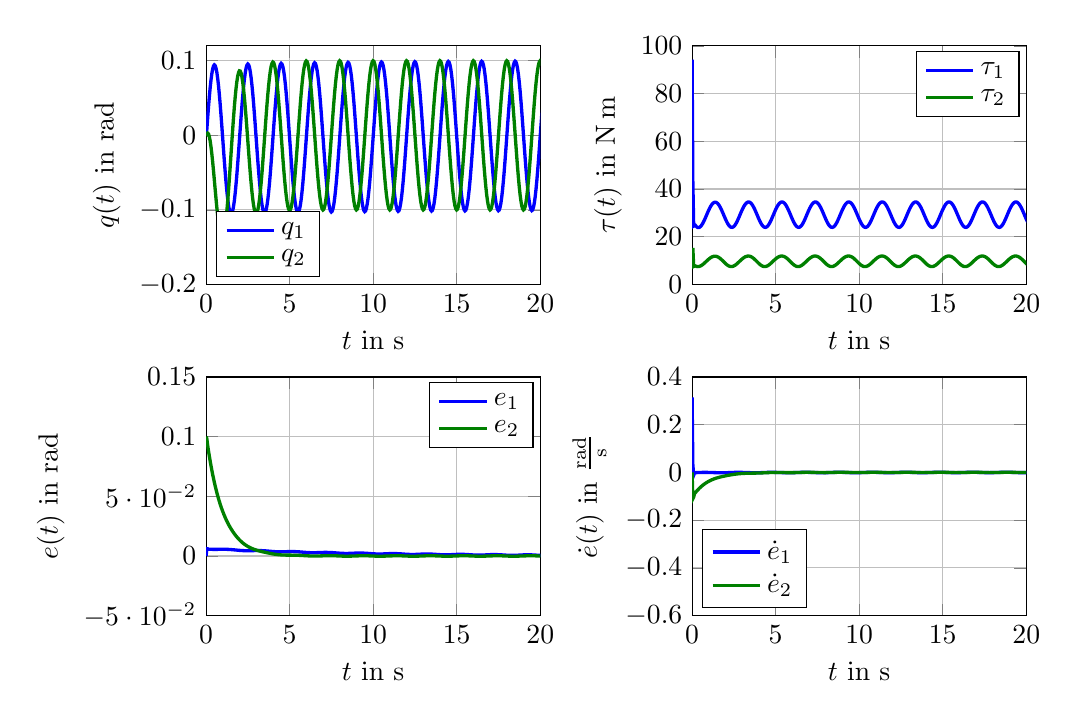
\begin{tikzpicture}

\begin{axis}[%
width=0.35\textwidth,
height=0.25\textwidth,
scale only axis,
xmin=0,
xmax=20,
xlabel={$t$ in $\mathrm{s}$},
xmajorgrids,
ymin=-0.2,
ymax=0.12,
ylabel={$q(t)$ in $\mathrm{rad}$},
ymajorgrids,
name=plot1,
legend style={at={(0.03,0.03)},anchor=south west,draw=black,fill=white,legend cell align=left}
]
\addplot [
color=blue,
solid,
line width=1.2pt
]
table[row sep=crcr]{
0 0\\
0.0447233782535311 0.00785895747901411\\
0.0947233782535311 0.023252789524387\\
0.144723378253531 0.0381869872538217\\
0.194723378253531 0.0517537646962405\\
0.244723378253531 0.0638851977106892\\
0.294723378253531 0.0743072935403581\\
0.344723378253531 0.0827550030389574\\
0.394723378253531 0.0890199798302507\\
0.444723378253531 0.0929489521203362\\
0.494723378253531 0.0944459610269336\\
0.544723378253531 0.0934749545903158\\
0.594723378253532 0.0900607301839733\\
0.644723378253532 0.08428830152798\\
0.694723378253532 0.0763007791260067\\
0.744723378253532 0.0662958173697892\\
0.794723378253532 0.0545207178258181\\
0.844723378253532 0.0412663140974768\\
0.894723378253532 0.0268597929522245\\
0.944723378253532 0.0116566310285948\\
0.994723378253532 -0.00396815368945291\\
1.04472337825353 -0.0196292215193527\\
1.09472337825352 -0.0349403777657606\\
1.14472337825352 -0.0495240572960999\\
1.19472337825351 -0.0630205976565927\\
1.24472337825351 -0.0750970760461712\\
1.2947233782535 -0.0854554950280185\\
1.34472337825349 -0.0938401163435307\\
1.39472337825349 -0.100043761573004\\
1.44472337825348 -0.103912922513256\\
1.49472337825348 -0.105351552682311\\
1.54472337825347 -0.104323443749382\\
1.59472337825347 -0.100853126107038\\
1.64472337825346 -0.0950252702052395\\
1.69472337825346 -0.0869826034457085\\
1.74472337825345 -0.0769223951203142\\
1.79472337825344 -0.0650915978516457\\
1.84472337825344 -0.0517807671949507\\
1.89472337825343 -0.0373169106475058\\
1.94472337825343 -0.0220554426882176\\
1.99472337825342 -0.00637144326328342\\
2.04472337825342 0.00934956686154795\\
2.09472337825341 0.0247211093473808\\
2.14472337825341 0.0393652594299821\\
2.1947233782534 0.0529219531238178\\
2.24472337825339 0.0650578625858745\\
2.29472337825339 0.0754746208795651\\
2.34472337825338 0.0839161917695309\\
2.39472337825338 0.0901751998077401\\
2.44472337825337 0.094098060678177\\
2.49472337825337 0.0955887811768\\
2.54472337825336 0.0946113316781611\\
2.59472337825336 0.0911905305647331\\
2.64472337825335 0.0854114187057209\\
2.69472337825335 0.0774171413347548\\
2.74472337825334 0.067405393201304\\
2.79472337825333 0.0556235193452837\\
2.84472337825333 0.0423623971465011\\
2.89472337825332 0.0279492545778692\\
2.94472337825332 0.012739604284507\\
2.99472337825331 -0.00289150707462393\\
3.04472337825331 -0.0185587199462403\\
3.0947233782533 -0.0338758293027015\\
3.1447233782533 -0.0484652692135955\\
3.19472337825329 -0.0619673852847628\\
3.24472337825328 -0.0740492703944035\\
3.29472337825328 -0.0844129487488112\\
3.34472337825327 -0.0928027077816099\\
3.39472337825327 -0.0990113968043784\\
3.44472337825326 -0.102885535436651\\
3.49472337825326 -0.104329103367553\\
3.54472337825325 -0.103305915364106\\
3.59472337825325 -0.099840520825684\\
3.64472337825324 -0.0940176045460526\\
3.69472337825324 -0.0859799034796536\\
3.74472337825323 -0.0759246919528044\\
3.79472337825322 -0.0640989237011755\\
3.84472337825322 -0.0507931522934996\\
3.89472337825321 -0.0363343810792089\\
3.94472337825321 -0.0210780191781031\\
3.9947233782532 -0.00539914083721355\\
4.04472337825322 0.0103167384944254\\
4.09472337825323 0.0256831448843078\\
4.14472337825325 0.0403221567530899\\
4.19472337825327 0.0538737119843446\\
4.24472337825328 0.0660044833923551\\
4.2947233782533 0.0764161037541426\\
4.34472337825332 0.0848525359905324\\
4.39472337825333 0.0911064037026587\\
4.44472337825335 0.0950241219737481\\
4.49472337825337 0.0965096977572054\\
4.54472337825338 0.0955271026542248\\
4.5947233782534 0.0921011575216526\\
4.64472337825342 0.0863169069785529\\
4.69472337825343 0.0783175011615035\\
4.74472337825345 0.0683006406222832\\
4.79472337825347 0.0565136767510107\\
4.84472337825348 0.0432474934192186\\
4.8947233782535 0.0288293248174553\\
4.94472337825352 0.0136146891518473\\
4.99472337825353 -0.00202136232955838\\
5.04472337825355 -0.0176934666812168\\
5.09472337825357 -0.0330154168032214\\
5.14472337825358 -0.0476096460339303\\
5.1947233782536 -0.0611165005164736\\
5.24472337825362 -0.0732030747839343\\
5.29472337825363 -0.0835713956051497\\
5.34472337825365 -0.091965753636632\\
5.39472337825367 -0.0981790018106616\\
5.44472337825368 -0.102057663508794\\
5.4947233782537 -0.103505722092027\\
5.54472337825372 -0.102486995718131\\
5.59472337825373 -0.0990260367563556\\
5.64472337825375 -0.0932075324662785\\
5.69472337825377 -0.0851742217369853\\
5.74472337825378 -0.0751233803214631\\
5.7947233782538 -0.0633019629374884\\
5.84472337825382 -0.0500005237821281\\
5.89472337825383 -0.0355460665837188\\
5.94472337825385 -0.0202940006962517\\
5.99472337825387 -0.00461940055011531\\
6.04472337825388 0.0110922181985323\\
6.0947233782539 0.026454381336306\\
6.14472337825392 0.041089166906144\\
6.19472337825393 0.0546365123204453\\
6.24472337825395 0.066763089855944\\
6.29472337825397 0.0771705317318499\\
6.34472337825398 0.0856028003499303\\
6.394723378254 0.0918525188958091\\
6.44472337825402 0.0957661022037633\\
6.49472337825403 0.0972475571987083\\
6.54472337825405 0.0962608557122235\\
6.59472337825407 0.0928308191086629\\
6.64472337825408 0.0870424927873783\\
6.6947233782541 0.0790390279112194\\
6.74472337825412 0.0690181262576181\\
6.79472337825414 0.0572271405800351\\
6.84472337825415 0.0439569561803396\\
6.89472337825417 0.0295348086732989\\
6.94472337825419 0.014316217613845\\
6.9947233782542 -0.00132376453687754\\
7.04472337825422 -0.0169997738035178\\
7.09472337825424 -0.0323256022724689\\
7.14472337825425 -0.0469236827020528\\
7.19472337825427 -0.0604343608921767\\
7.24472337825429 -0.0725247312601212\\
7.2947233782543 -0.0828968206669524\\
7.34472337825432 -0.091294920042981\\
7.39472337825434 -0.0975118827453497\\
7.44472337825435 -0.101394232699881\\
7.49472337825437 -0.102845953900978\\
7.54472337825439 -0.101830865202089\\
7.5947233782544 -0.0983735197083105\\
7.64472337825442 -0.0925586054384501\\
7.69472337825444 -0.084528862052644\\
7.74472337825445 -0.0744815660796002\\
7.79472337825447 -0.0626636730135429\\
7.84472337825449 -0.0493657378265276\\
7.8947233782545 -0.0349147650185646\\
7.94472337825452 -0.0196661647092575\\
7.99472337825454 -0.00399501208402627\\
8.04472337825451 0.0117131764633075\\
8.09472337825449 0.0270719260082362\\
8.14472337825446 0.0417033139204787\\
8.19472337825443 0.0552472769902235\\
8.2447233782544 0.0673704869372321\\
8.29472337825437 0.0777745755035733\\
8.34472337825435 0.0862035047078081\\
8.39472337825432 0.0924498974589743\\
8.44472337825429 0.0963601684316886\\
8.49472337825426 0.0978383245151262\\
8.54472337825424 0.0968483376319077\\
8.59472337825421 0.0934150293623278\\
8.64472337825418 0.0876234454396475\\
8.69472337825415 0.0796167374666847\\
8.74472337825413 0.0695926077504749\\
8.7947233782541 0.0577984096436195\\
8.84472337825407 0.0445250290940097\\
8.89472337825404 0.0300997023853886\\
8.94472337825401 0.0148779497407273\\
8.99472337825399 -0.000765175734376394\\
9.04472337825396 -0.0164443094641192\\
9.09472337825393 -0.03177324299591\\
9.1447233782539 -0.0463744086246589\\
9.19472337825388 -0.059888151773054\\
9.24472337825385 -0.0719815665746089\\
9.29472337825382 -0.0823566797042858\\
9.34472337825379 -0.0907577820055413\\
9.39472337825377 -0.0969777268473402\\
9.44472337825374 -0.100863038263711\\
9.49472337825371 -0.102317700449992\\
9.54472337825368 -0.10130553254851\\
9.59472337825365 -0.0978510880353916\\
9.64472337825363 -0.0920390553758038\\
9.6947233782536 -0.0840121747436512\\
9.74472337825357 -0.0739677232396865\\
9.79472337825354 -0.0621526569780418\\
9.84472337825352 -0.0488575315868675\\
9.89472337825349 -0.0344093522456494\\
9.94472337825346 -0.0191635297631709\\
9.99472337825343 -0.0034951400095571\\
10.0447233782534 0.0122102999553881\\
10.0947233782534 0.0275663145737594\\
10.1447233782533 0.0421949806275105\\
10.1947233782533 0.0557362343765657\\
10.2447233782533 0.0678567470783205\\
10.2947233782533 0.0782581500890965\\
10.3447233782532 0.0866844051252176\\
10.3947233782532 0.0929281348819509\\
10.4447233782532 0.0968357539115349\\
10.4947233782532 0.0983112690729624\\
10.5447233782531 0.097318652349461\\
10.5947233782531 0.0938827254690295\\
10.6447233782531 0.0880885343937289\\
10.694723378253 0.080079231028007\\
10.744723378253 0.0700525180429898\\
10.794723378253 0.0582557492056279\\
10.844723378253 0.0449798109147926\\
10.8947233782529 0.0305519399272764\\
10.9447233782529 0.0153276569462374\\
10.9947233782529 -0.00031798445013291\\
11.0447233782529 -0.0159996192350294\\
11.0947233782528 -0.0313310385392656\\
11.1447233782528 -0.0459346742868629\\
11.1947233782528 -0.0594508715849051\\
11.2447233782527 -0.0715467243143624\\
11.2947233782527 -0.0819242589667042\\
11.3447233782527 -0.0903277662752386\\
11.3947233782527 -0.0965500995748334\\
11.4447233782526 -0.100437782942695\\
11.4947233782526 -0.101894800694414\\
11.5447233782526 -0.10088497216804\\
11.5947233782525 -0.0974328511078195\\
11.6447233782525 -0.0916231263148624\\
11.6947233782525 -0.0835985383606653\\
11.7447233782525 -0.0735563647974587\\
11.7947233782524 -0.0617435622354368\\
11.8447233782524 -0.0484506868327293\\
11.8947233782524 -0.0340047443209634\\
11.9447233782524 -0.0187611460707543\\
11.9947233782523 -0.0030949685109973\\
12.0447233782523 0.0126082707553698\\
12.0947233782523 0.027962095654904\\
12.1447233782522 0.0425885824925855\\
12.1947233782522 0.0561276670996089\\
12.2447233782522 0.0682460203610743\\
12.2947233782522 0.0786452733240258\\
12.3447233782521 0.0870693874634607\\
12.3947233782521 0.0933109853045456\\
12.4447233782521 0.0972164813022796\\
12.494723378252 0.0986898822912851\\
12.544723378252 0.0976951603016715\\
12.594723378252 0.0942571371763283\\
12.644723378252 0.0884608590553524\\
12.6947233782519 0.0804494780779279\\
12.7447233782519 0.0704206971986851\\
12.7947233782519 0.0586218705075999\\
12.8447233782519 0.0453438847557771\\
12.8947233782518 0.0309139770704074\\
12.9447233782518 0.0156876685318142\\
12.9947233782518 4.00130907793558e-05\\
13.0447233782517 -0.0156436238687709\\
13.0947233782517 -0.0309770331461046\\
13.1447233782517 -0.0455826463683218\\
13.1947233782517 -0.059100808388022\\
13.2447233782516 -0.0711986128806146\\
13.2947233782516 -0.081578086186079\\
13.3447233782516 -0.089983518944142\\
13.3947233782515 -0.0962077644565881\\
13.4447233782515 -0.100097346829424\\
13.4947233782515 -0.101556250469128\\
13.5447233782515 -0.10054829486573\\
13.5947233782514 -0.0970980339743003\\
13.6447233782514 -0.0912901568620687\\
13.6947233782514 -0.0832674044170259\\
13.7447233782514 -0.0732270545519927\\
13.7947233782513 -0.0614160642742745\\
13.8447233782513 -0.0481249901669169\\
13.8947233782513 -0.0336808384046559\\
13.9447233782512 -0.0184390208092218\\
13.9947233782512 -0.00277461425823687\\
14.0447233782512 0.012926863209243\\
14.0947233782512 0.0282789351059544\\
14.1447233782511 0.0429036773542018\\
14.1947233782511 0.0564410254414211\\
14.2447233782511 0.0685576499544066\\
14.294723378251 0.0789551816925667\\
14.344723378251 0.087377581937802\\
14.394723378251 0.0936174730792514\\
14.444723378251 0.0975212694941693\\
14.4947233782509 0.0989929779976378\\
14.5447233782509 0.0979965706570717\\
14.5947233782509 0.0945568694068783\\
14.6447233782509 0.0887589205289841\\
14.6947233782508 0.0807458763495797\\
14.7447233782508 0.0707154400491798\\
14.7947233782508 0.0589149659751889\\
14.8447233782507 0.0456353411595124\\
14.8947233782507 0.031203803024752\\
14.9447233782507 0.0159758729522044\\
14.9947233782507 0.00032660519016712\\
15.0447233782506 -0.0153586345920566\\
15.0947233782506 -0.0306936369285675\\
15.1447233782506 -0.0453008332087525\\
15.1947233782506 -0.0588205680812281\\
15.2447233782505 -0.07091993505638\\
15.2947233782505 -0.0813009603522903\\
15.3447233782505 -0.0897079345330436\\
15.3947233782504 -0.0959337108731662\\
15.4447233782504 -0.0998248135009536\\
15.4947233782504 -0.101285226894934\\
15.5447233782504 -0.100278770666183\\
15.5947233782503 -0.0968299989380535\\
15.6447233782503 -0.0910236009904516\\
15.6947233782503 -0.0830023179645108\\
15.7447233782502 -0.0729634280616229\\
15.7947233782502 -0.0611538886070089\\
15.8447233782502 -0.0478642565239726\\
15.8947233782502 -0.0334215383421291\\
15.9447233782501 -0.0181811462445264\\
15.9947233782501 -0.00251815746819688\\
16.0447233782502 0.0131819095985037\\
16.0947233782502 0.028532578136891\\
16.1447233782503 0.0431559237628198\\
16.1947233782503 0.0566918816884708\\
16.2447233782504 0.0688071222618071\\
16.2947233782505 0.0792032760839976\\
16.3447233782505 0.0876243042823811\\
16.3947233782506 0.0938628291372245\\
16.4447233782506 0.0977652649635587\\
16.4947233782507 0.0992356185608173\\
16.5447233782508 0.0982378620262453\\
16.5947233782508 0.0947968173674459\\
16.6447233782509 0.0889975309797851\\
16.694723378251 0.0809831553390302\\
16.744723378251 0.0709513938063739\\
16.7947233782511 0.0591496009351412\\
16.8447233782511 0.0458686639818678\\
16.8947233782512 0.0314358206054949\\
16.9447233782513 0.016206592428133\\
16.9947233782513 0.000556033936156299\\
17.0447233782514 -0.0151304889727381\\
17.0947233782514 -0.0304667666203979\\
17.1447233782515 -0.0450752302058995\\
17.1947233782516 -0.0585962242145184\\
17.2447233782516 -0.0706968420244608\\
17.2947233782517 -0.0810791097561349\\
17.3447233782517 -0.0894873179129685\\
17.3947233782518 -0.0957143197475614\\
17.4447233782519 -0.0996066394059521\\
17.4947233782519 -0.101068261424256\\
17.544723378252 -0.100063005510378\\
17.5947233782521 -0.0966154259223316\\
17.6447233782521 -0.0908102121102423\\
17.6947233782522 -0.0827901054178786\\
17.7447233782522 -0.0727523842776446\\
17.7947233782523 -0.0609440062692793\\
17.8447233782524 -0.0476555285884997\\
17.8947233782524 -0.033213958049044\\
17.9447233782525 -0.0179747071232384\\
17.9947233782525 -0.00231285333586387\\
18.0447233782526 0.0133860846450735\\
18.0947233782527 0.0287356297355608\\
18.1447233782527 0.0433578573061225\\
18.1947233782528 0.0568927023485881\\
18.2447233782528 0.0690068350197333\\
18.2947233782529 0.0794018857620385\\
18.344723378253 0.0878218155791209\\
18.394723378253 0.0940592466641004\\
18.4447233782531 0.0979605932822024\\
18.4947233782532 0.0994298622203349\\
18.5447233782532 0.098431025599618\\
18.5947233782533 0.0949889054862401\\
18.6447233782533 0.0891885483663634\\
18.6947233782534 0.081173106835475\\
18.7447233782535 0.0711402843993829\\
18.7947233782535 0.0593374357762334\\
18.8447233782536 0.0460554484023625\\
18.8947233782536 0.031621560125888\\
18.9447233782537 0.0163912927616839\\
18.9947233782538 0.000739700986701762\\
19.0447233782538 -0.0149478491185289\\
19.0947233782539 -0.0302851477059387\\
19.1447233782539 -0.0448946258222474\\
19.194723378254 -0.058416627821959\\
19.2447233782541 -0.0705182469774515\\
19.2947233782541 -0.0809015093309255\\
19.3447233782542 -0.0893107053372354\\
19.3947233782543 -0.0955386882314132\\
19.4447233782543 -0.0994319821736886\\
19.4947233782544 -0.100894571746269\\
19.5447233782544 -0.0998902767345712\\
19.5947233782545 -0.0964436515044038\\
19.6447233782546 -0.0906393856421648\\
19.6947233782546 -0.0826202206538426\\
19.7447233782547 -0.0725834351567826\\
19.7947233782547 -0.0607759869344822\\
19.8447233782548 -0.047488433400743\\
19.8947233782549 -0.0330477815967608\\
19.9447233782549 -0.0178094442264449\\
19.994723378255 -0.00214849904493269\\
20.044723378255 0.0135495350558991\\
20.0947233782551 0.0288981807796329\\
20.1447233782552 0.0435195133003999\\
20.1947233782552 0.057053467433634\\
20.2447233782553 0.0691667131830634\\
20.2947233782554 0.0795608808641374\\
20.3447233782554 0.0879799313814333\\
20.3947233782555 0.0942164868583103\\
20.4447233782555 0.0981169615201238\\
20.4947233782556 0.0995853621437537\\
20.5447233782557 0.0985856608694307\\
20.5947233782557 0.0951426798102387\\
20.6447233782558 0.0893414655250194\\
20.6947233782558 0.0813251707050935\\
20.7447233782559 0.0712914989720319\\
20.794723378256 0.0594878051759197\\
20.844723378256 0.0462049768970244\\
20.8947233782561 0.0317702521349026\\
20.9447233782561 0.0165391528587406\\
20.9947233782562 0.000886733898053935\\
21.0447233782563 -0.0148016385202617\\
21.0947233782563 -0.0301397544121086\\
21.1447233782564 -0.0447500447022342\\
21.1947233782565 -0.0582728536404495\\
21.2447233782565 -0.0703752744144071\\
21.2947233782566 -0.0807593330036939\\
21.3447233782566 -0.0891693198242748\\
21.3947233782567 -0.0953980880971145\\
21.4447233782568 -0.0992921619938022\\
21.4947233782568 -0.100755526133443\\
21.5447233782569 -0.0997520003635061\\
21.5947233782569 -0.0963061391360993\\
21.644723378257 -0.0905026321467142\\
21.6947233782571 -0.0824842210312089\\
21.7447233782571 -0.072448184554986\\
21.7947233782572 -0.0606414806646648\\
21.8447233782572 -0.0473546669486364\\
21.8947233782573 -0.0329147506301886\\
21.9447233782574 -0.017677144598624\\
21.9947233782574 -0.00201692679348961\\
22.0447233782575 0.0136803837141211\\
22.0947233782576 0.0290283094577548\\
22.1447233782576 0.0436489254543247\\
22.1947233782577 0.0571821663780571\\
22.2447233782577 0.0692947021101634\\
22.2947233782578 0.079688162864403\\
22.3447233782579 0.088106509466071\\
22.3947233782579 0.0943423639826824\\
22.444723378258 0.0982421406076761\\
22.494723378258 0.0997098461099041\\
22.5447233782581 0.0987094526448948\\
22.5947233782582 0.0952657823632712\\
22.6447233782582 0.0894638818820552\\
22.6947233782583 0.0814469039692828\\
22.7447233782583 0.0714125523391945\\
22.7947233782584 0.0596081819474946\\
22.8447233782585 0.0463246804896712\\
22.8947233782585 0.0318892860865122\\
22.9447233782586 0.0166575208307363\\
22.9947233782587 0.00100443967399343\\
23.0447233782587 -0.0146845910396474\\
23.0947233782588 -0.03002336121719\\
23.1447233782588 -0.0446343016857352\\
23.1947233782589 -0.0581577566112802\\
23.244723378259 -0.0702608191136483\\
23.294723378259 -0.0806455151222994\\
23.3447233782591 -0.0890561350220634\\
23.3947233782591 -0.095285532022643\\
23.4447233782592 -0.0991802303047205\\
23.4947233782593 -0.100644214516941\\
23.5447233782593 -0.0996413045564498\\
23.5947233782594 -0.0961960549444441\\
23.6447233782594 -0.0903931554637529\\
23.6947233782595 -0.082375347854203\\
23.7447233782596 -0.0723399109997269\\
23.7947233782596 -0.0605338029775324\\
23.8447233782597 -0.0472475815157792\\
23.8947233782598 -0.032808253983529\\
23.9447233782598 -0.0175712334185\\
23.9947233782599 -0.0019115979078667\\
24.0447233782599 0.0137851333338084\\
24.09472337826 0.0291324827039528\\
24.1447233782601 0.0437525250936231\\
24.1947233782601 0.0572851950640057\\
24.2447233782602 0.0693971623982349\\
24.2947233782602 0.0797900572286657\\
24.3447233782603 0.0882078403171273\\
24.3947233782604 0.09444313368643\\
24.4447233782604 0.0983423515044636\\
24.4947233782605 0.0998095005336534\\
24.5447233782605 0.0988085529417739\\
24.5947233782606 0.0953643309094983\\
24.6447233782607 0.0895618811004226\\
24.6947233782607 0.0815443563439947\\
24.7447233782608 0.0715094604286388\\
24.7947233782609 0.0597045483946104\\
24.8447233782609 0.0464205080296347\\
24.894723378261 0.0319845775515496\\
24.944723378261 0.0167522791519665\\
24.9947233782611 0.00109866788030917\\
25.0447233782612 -0.0145908898255505\\
25.0947233782612 -0.0299301837854371\\
25.1447233782613 -0.04454164474828\\
25.1947233782613 -0.0580656168129779\\
25.2447233782614 -0.0701691930450525\\
25.2947233782615 -0.0805543993338335\\
25.3447233782615 -0.0889655260392252\\
25.3947233782616 -0.0951954263619141\\
25.4447233782616 -0.0990906244898623\\
25.4947233782617 -0.100555105095363\\
25.5447233782618 -0.0995526881153324\\
25.5947233782618 -0.0961079281262772\\
25.6447233782619 -0.0903055149809461\\
25.694723378262 -0.0822881905023999\\
25.744723378262 -0.0722532336694611\\
25.7947233782621 -0.0604476026638811\\
25.8447233782621 -0.0471618553257121\\
25.8947233782622 -0.0327229991407147\\
25.9447233782623 -0.0174864472654203\\
25.9947233782623 -0.00182727790518532\\
26.0447233782624 0.0138689896105756\\
26.0947233782624 0.0292158775703224\\
26.1447233782625 0.0438354607643598\\
26.1947233782626 0.057367673663383\\
26.2447233782626 0.0694791859720135\\
26.2947233782627 0.0798716277574408\\
26.3447233782627 0.088288959730688\\
26.3947233782628 0.0945238038787794\\
26.4447233782629 0.0984225743491521\\
26.4947233782629 0.0998892778990869\\
26.544723378263 0.0988878867061614\\
26.5947233782631 0.0954432229751051\\
26.6447233782631 0.0896403334067975\\
26.6947233782632 0.0816223708798481\\
26.7447233782632 0.0715870392420676\\
26.7947233782633 0.0597816936013968\\
26.8447233782634 0.0464972218194002\\
26.8947233782634 0.0320608621916076\\
26.9447233782635 0.0168281369887978\\
26.9947233782635 0.00117410133866697\\
27.0447233782636 -0.0145158782458193\\
27.0947233782637 -0.0298555915146943\\
27.1447233782637 -0.0444674691543068\\
27.1947233782638 -0.0579918552098394\\
27.2447233782638 -0.0700958427033424\\
27.2947233782639 -0.0804814574920187\\
27.344723378264 -0.0888929899158182\\
27.394723378264 -0.0951232931682096\\
27.4447233782641 -0.0990188914429832\\
27.4947233782642 -0.100483769431365\\
27.5447233782642 -0.0994817471021088\\
27.5947233782643 -0.0960373790760019\\
27.6447233782643 -0.0902353552617676\\
27.6947233782644 -0.0822184175491006\\
27.7447233782645 -0.0721838449927887\\
27.7947233782645 -0.0603785958582762\\
27.8447233782646 -0.0470932280751907\\
27.8947233782646 -0.0326547492227162\\
27.9447233782647 -0.0174185725524993\\
27.9947233782648 -0.0017597763645056\\
28.0447233782648 0.0139361199199067\\
28.0947233782649 0.0292826385019656\\
28.1447233782649 0.0439018540913207\\
28.194723378265 0.0574337010862265\\
28.2447233782651 0.0695448491284534\\
28.2947233782651 0.0799369282330243\\
28.3447233782652 0.0883538990702914\\
28.3947233782653 0.0945883835986317\\
28.4447233782653 0.0984867959491097\\
28.4947233782654 0.0999531428748884\\
28.5447233782654 0.0989513965613931\\
28.5947233782655 0.0955063792326113\\
28.6447233782656 0.0897031376192692\\
28.6947233782656 0.0816848246393318\\
28.7447233782657 0.0716491441881502\\
28.7947233782657 0.0598434514278502\\
28.8447233782658 0.0465586342791069\\
28.8947233782659 0.0321219310996456\\
28.9447233782659 0.0168888642236221\\
28.994723378266 0.00123448884139289\\
29.044723378266 -0.0144558284739604\\
29.0947233782661 -0.0297958774165999\\
29.1447233782662 -0.0444080886227754\\
29.1947233782662 -0.057932806094667\\
29.2447233782663 -0.0700371228195238\\
29.2947233782664 -0.0804230646288297\\
29.3447233782664 -0.0888349218465601\\
29.3947233782665 -0.0950655476604059\\
29.4447233782665 -0.0989614662688232\\
29.4947233782666 -0.100426662378195\\
29.5447233782667 -0.0994249559827642\\
29.5947233782667 -0.0959809017387669\\
29.6447233782668 -0.0901791895997382\\
29.6947233782668 -0.0821625615087171\\
29.7447233782669 -0.0721282965813056\\
29.794723378267 -0.0603233531499491\\
29.844723378267 -0.0470382892159848\\
29.8947233782671 -0.0326001124333863\\
29.9447233782671 -0.0173642361299442\\
29.9947233782672 -0.00170573868136295\\
30.0447233782673 0.0139898604173953\\
30.0947233782673 0.0293360832977261\\
30.1447233782674 0.0439550046047123\\
30.1947233782675 0.0574865586786177\\
30.2447233782675 0.0695974151108986\\
30.2947233782676 0.0799892038748175\\
30.3447233782676 0.0884058856081688\\
30.3947233782677 0.0946400822463968\\
30.4447233782678 0.0985382079074599\\
30.4947233782678 0.100004269341225\\
30.5447233782679 0.0990022387394002\\
30.5947233782679 0.09555693834139\\
30.644723378268 0.0897534149018138\\
30.6947233782681 0.0817348213701424\\
30.7447233782681 0.071698861679785\\
30.7947233782682 0.0598928910362441\\
30.8447233782682 0.0466077974075155\\
30.8947233782683 0.0321708192011145\\
30.9447233782684 0.0169374788019328\\
30.9947233782684 0.00128283145048917\\
31.0447233782685 -0.0144077562320091\\
31.0947233782686 -0.0297480738949965\\
31.1447233782686 -0.0443605521346164\\
31.1947233782687 -0.0578855349186235\\
31.2447233782687 -0.0699901152064066\\
31.2947233782688 -0.0803763188088606\\
31.3447233782689 -0.0887884360371729\\
31.3947233782689 -0.095019320074409\\
31.444723378269 -0.0989154951227609\\
31.494723378269 -0.100380945900746\\
31.5447233782691 -0.0993794924230132\\
31.5947233782692 -0.0959356893741777\\
31.6447233782692 -0.090134226743649\\
31.6947233782693 -0.0821178465171715\\
31.7447233782693 -0.0720838278590327\\
31.7947233782694 -0.0602791291553157\\
31.8447233782695 -0.0469943084647649\\
31.8947233782695 -0.0325563735012266\\
31.9447233782696 -0.0173207376534483\\
31.9947233782697 -0.00166247935776605\\
32.0447233782696 0.0140328818319348\\
32.0947233782694 0.0293788679911484\\
32.1447233782693 0.0439975537132728\\
32.1947233782692 0.0575288732921508\\
32.2447233782691 0.069639496278963\\
32.294723378269 0.0800310526135434\\
32.3447233782689 0.0884475029076242\\
32.3947233782687 0.0946814690782924\\
32.4447233782686 0.0985793652330145\\
32.4947233782685 0.100045198119018\\
32.5447233782684 0.0990429399330404\\
32.5947233782683 0.095597412926825\\
32.6447233782682 0.0897936638741164\\
32.694723378268 0.0817748457496038\\
32.7447233782679 0.0717386625171595\\
32.7947233782678 0.0599324694170071\\
32.8447233782677 0.0466471544550204\\
32.8947233782676 0.0322099560785694\\
32.9447233782675 0.0169763967131583\\
32.9947233782673 0.00132153163945922\\
33.0447233782672 -0.0143692724827968\\
33.0947233782671 -0.0297098052672405\\
33.144723378267 -0.0443224972779097\\
33.1947233782669 -0.0578476924550009\\
33.2447233782668 -0.0699524837355996\\
33.2947233782666 -0.080338896914117\\
33.3447233782665 -0.0887512222915015\\
33.3947233782664 -0.0949823130471125\\
33.4447233782663 -0.0988786933861295\\
33.4947233782662 -0.100344348036779\\
33.5447233782661 -0.0993430970300404\\
33.5947233782659 -0.095899495073242\\
33.6447233782658 -0.0900982321845058\\
33.6947233782657 -0.0820820503837571\\
33.7447233782656 -0.0720482288742515\\
33.7947233782655 -0.0602437260850043\\
33.8447233782654 -0.0469591001207104\\
33.8947233782652 -0.0325213587431406\\
33.9447233782651 -0.0172859153898351\\
33.994723378265 -0.00162784854566382\\
34.0447233782649 0.0140673221883216\\
34.0947233782648 0.0294131188428631\\
34.1447233782647 0.0440316159699785\\
34.1947233782645 0.0575627478263445\\
34.2447233782644 0.069673183930894\\
34.2947233782643 0.0800645541966939\\
34.3447233782642 0.0884808192146059\\
34.3947233782641 0.0947146008870144\\
34.444723378264 0.0986123133129795\\
34.4947233782638 0.100077963237609\\
34.5447233782637 0.0990755228616591\\
34.5947233782636 0.095629814446745\\
34.6447233782635 0.0898258847819159\\
34.6947233782634 0.0818068868620443\\
34.7447233782633 0.0717705246753855\\
34.7947233782631 0.0599641534899553\\
34.844723378263 0.0466786613419484\\
34.8947233782629 0.0322412867106391\\
34.9447233782628 0.0170075520540432\\
34.9947233782627 0.00135251268497841\\
35.0447233782626 -0.0143384647059828\\
35.0947233782624 -0.0296791697038059\\
35.1447233782623 -0.0442920328468238\\
35.1947233782622 -0.0578173980531677\\
35.2447233782621 -0.0699223582420643\\
35.294723378262 -0.0803089391947246\\
35.3447233782619 -0.0887214312038956\\
35.3947233782617 -0.094952687445966\\
35.4447233782616 -0.0988492321285022\\
35.4947233782615 -0.1003150499875\\
35.5447233782614 -0.0993139610670098\\
35.5947233782613 -0.0958705200925387\\
35.6447233782612 -0.090069417105193\\
35.694723378261 -0.0820533941522596\\
35.7447233782609 -0.0720197304681888\\
35.7947233782608 -0.0602153845163651\\
35.8447233782607 -0.0469309144382689\\
35.8947233782606 -0.0324933280340374\\
35.9447233782605 -0.017258038780273\\
35.9947233782603 -0.00160012520070031\\
36.0447233782602 0.0140948930658682\\
36.0947233782601 0.0294405380143478\\
36.14472337826 0.0440588841636304\\
36.1947233782599 0.057589865740639\\
36.2447233782598 0.0697001522384905\\
36.2947233782596 0.0800913735488234\\
36.3447233782595 0.0885074902457909\\
36.3947233782594 0.0947411242200061\\
36.4447233782593 0.098638689563799\\
36.4947233782592 0.100104193020579\\
36.5447233782591 0.0991016067943183\\
36.5947233782589 0.0956557531545338\\
36.6447233782588 0.0898516789025255\\
36.6947233782587 0.0818325370493218\\
36.7447233782586 0.0717960316026968\\
36.7947233782585 0.059989517852914\\
36.8447233782584 0.0467038838604401\\
36.8947233782582 0.0322663681300896\\
36.9447233782581 0.0170324931459047\\
36.994723378258 0.00137731424643658\\
37.0447233782579 -0.0143138018530525\\
37.0947233782578 -0.0296546447145802\\
37.1447233782577 -0.0442676448559012\\
37.1947233782575 -0.057793146177482\\
37.2447233782574 -0.0698982415842519\\
37.2947233782573 -0.0802849568468538\\
37.3447233782572 -0.088697582251468\\
37.3947233782571 -0.0949289709721043\\
37.444723378257 -0.0988256472182391\\
37.4947233782569 -0.100291595732087\\
37.5447233782567 -0.0992906365681589\\
37.5947233782566 -0.0958473244665163\\
37.6447233782565 -0.0900463494866634\\
37.6947233782564 -0.0820304536977905\\
37.7447233782563 -0.0719969163593196\\
37.7947233782562 -0.0601926959621482\\
37.844723378256 -0.0469083506772043\\
37.8947233782559 -0.0324708883353387\\
37.9447233782558 -0.0172357224444238\\
37.9947233782557 -0.00157793155928892\\
38.0447233782556 0.0141169646510247\\
38.0947233782555 0.0294624881527516\\
38.1447233782553 0.0440807134382648\\
38.1947233782552 0.0576115747106683\\
38.2447233782551 0.0697217414424116\\
38.294723378255 0.0801128435079782\\
38.3447233782549 0.0885288414681447\\
38.3947233782548 0.0947623572041003\\
38.4447233782546 0.0986598048027857\\
38.4947233782545 0.10012519100625\\
38.5447233782544 0.0991224880210383\\
38.5947233782543 0.0956765181229923\\
38.6447233782542 0.0898723281232178\\
38.6947233782541 0.0818530710456758\\
38.7447233782539 0.0718164509137645\\
38.7947233782538 0.0600098230355569\\
38.8447233782537 0.0467240754909497\\
38.8947233782536 0.0322864468052023\\
38.9447233782535 0.0170524594831918\\
38.9947233782534 0.00139716888406991\\
39.0447233782532 -0.0142940582571361\\
39.0947233782531 -0.0296350114840732\\
39.144723378253 -0.044248121298022\\
39.1947233782529 -0.0577737315853072\\
39.2447233782528 -0.0698789352394116\\
39.2947233782527 -0.0802657580225174\\
39.3447233782525 -0.0886784902155472\\
39.3947233782524 -0.0949099849906049\\
39.4447233782523 -0.0988067665586951\\
39.4947233782522 -0.100272819667009\\
39.5447233782521 -0.099271964378433\\
39.594723378252 -0.0958287554446763\\
39.6447233782518 -0.0900278829399712\\
39.6947233782517 -0.0820120889510416\\
39.7447233782516 -0.0719786527572993\\
39.7947233782515 -0.0601745328716664\\
39.8447233782514 -0.0468902874886443\\
39.8947233782513 -0.0324529244636703\\
39.9447233782511 -0.0172178573296497\\
39.994723378251 -0.00156016466631185\\
40.0447233782509 0.0141346338331027\\
40.0947233782508 0.0294800601118685\\
40.1447233782507 0.044098188641129\\
40.1947233782506 0.0576289536049195\\
40.2447233782504 0.0697390244591444\\
40.2947233782503 0.0801300310645528\\
40.3447233782502 0.0885459339712124\\
40.3947233782501 0.0947793550527669\\
40.44472337825 0.0986767083918418\\
40.4947233782499 0.100142000729396\\
40.5447233782497 0.0991392042740336\\
40.5947233782496 0.0956931413066578\\
40.6447233782495 0.0898888586462235\\
40.6947233782494 0.0818695093270436\\
40.7447233782493 0.071832797385023\\
40.7947233782492 0.0600260781424908\\
40.844723378249 0.0467402396948973\\
40.8947233782489 0.0323025205838687\\
40.9447233782488 0.0170684433309605\\
40.9947233782487 0.00141306331181563\\
41.0447233782486 -0.0142782527227159\\
41.0947233782485 -0.0296192943015745\\
41.1447233782483 -0.0442324919128523\\
41.1947233782482 -0.0577581894315525\\
41.2447233782481 -0.0698634797419941\\
41.294723378248 -0.080250388599585\\
41.3447233782479 -0.0886632062810381\\
41.3947233782478 -0.0948947859569307\\
41.4447233782476 -0.0987916518394894\\
41.4947233782475 -0.100257788679889\\
41.5447233782474 -0.0992570165477185\\
41.5947233782473 -0.0958138902040117\\
41.6447233782472 -0.0900130997347896\\
41.6947233782471 -0.0819973872408116\\
41.7447233782469 -0.0719640320174913\\
41.7947233782468 -0.0601599925953813\\
41.8447233782467 -0.046875827187854\\
41.8947233782466 -0.0324385436700286\\
41.9447233782465 -0.0172035555948496\\
41.9947233782464 -0.00154594156197973\\
42.0447233782462 0.0141487787159682\\
42.0947233782461 0.0294941271638885\\
42.144723378246 0.0441121782359288\\
42.1947233782459 0.0576428661008594\\
42.2447233782458 0.0697528602013384\\
42.2947233782457 0.08014379038712\\
42.3447233782455 0.0885596171996978\\
42.3947233782454 0.0947929625066741\\
42.4447233782453 0.0986902403872192\\
42.4947233782452 0.100155457581418\\
42.5447233782451 0.0991525862995213\\
42.594723378245 0.0957064488264836\\
42.6447233782448 0.0899020919875419\\
42.6947233782447 0.0818826688252953\\
42.7447233782446 0.0718458833856595\\
42.7947233782445 0.0600390910023757\\
42.8447233782444 0.0467531797833446\\
42.8947233782443 0.0323153882832937\\
42.9447233782441 0.0170812390371302\\
42.994723378244 0.00142578743369835\\
43.0447233782439 -0.0142655997634851\\
43.0947233782438 -0.0296067120715872\\
43.1447233782437 -0.0442199799681421\\
43.1947233782436 -0.057745747319089\\
43.2447233782434 -0.0698511070014103\\
43.2947233782433 -0.0802380847650902\\
43.3447233782432 -0.0886509708834706\\
43.3947233782431 -0.0948826185259059\\
43.444723378243 -0.0987795519055999\\
43.4947233782429 -0.100245755776915\\
43.5447233782428 -0.0992450502148053\\
43.5947233782426 -0.0958019899877677\\
43.6447233782425 -0.0900012651912598\\
43.6947233782424 -0.0819856179372757\\
43.7447233782423 -0.0719523275340384\\
43.7947233782422 -0.0601483525262136\\
43.8447233782421 -0.0468642511422797\\
43.8947233782419 -0.0324270312731115\\
43.9447233782418 -0.0171921064876955\\
43.9947233782417 -0.00153455540165122\\
44.0447233782416 0.0141601022569002\\
44.0947233782415 0.0295053883981385\\
44.1447233782414 0.0441233774626061\\
44.1947233782412 0.0576540036068518\\
44.2447233782411 0.0697639362629297\\
44.294723378241 0.080154805271791\\
44.3447233782409 0.0885705711680646\\
44.3947233782408 0.0948038558145158\\
44.4447233782407 0.0987010732875474\\
44.4947233782405 0.100166230326544\\
44.5447233782404 0.0991632991430726\\
44.5947233782403 0.0957171020253309\\
44.6447233782402 0.0899126858035833\\
44.6947233782401 0.0818932035270611\\
44.74472337824 0.0718563592496936\\
44.7947233782398 0.0600495083143564\\
44.8447233782397 0.0467635388389167\\
44.8947233782396 0.0323256893885895\\
44.9447233782395 0.0170914825089699\\
44.9947233782394 0.00143597359947048\\
45.0447233782393 -0.0142554705662522\\
45.0947233782391 -0.02959663949594\\
45.144723378239 -0.0442099636586746\\
45.1947233782389 -0.0577357869131389\\
45.2447233782388 -0.0698412021304413\\
45.2947233782387 -0.0802282350562234\\
45.3447233782386 -0.0886411759611277\\
45.3947233782384 -0.0948728780135283\\
45.4447233782383 -0.0987698654274106\\
45.4947233782382 -0.100236122959688\\
45.5447233782381 -0.0992354706896072\\
45.594723378238 -0.0957924633916398\\
45.6447233782379 -0.0899917911687963\\
45.6947233782377 -0.0819761961420637\\
45.7447233782376 -0.0719429576299181\\
45.7947233782375 -0.0601390341883229\\
45.8447233782374 -0.0468549840578484\\
45.8947233782373 -0.0324178151419821\\
45.9447233782372 -0.0171829410225517\\
45.994723378237 -0.0015254403279513\\
46.0447233782369 0.0141691672012835\\
46.0947233782368 0.029514403463553\\
46.1447233782367 0.0441323428885072\\
46.1947233782366 0.0576629196229114\\
46.2447233782365 0.0697728030903298\\
46.2947233782363 0.0801636231246659\\
46.3447233782362 0.0885793402550524\\
46.3947233782361 0.0948125763403811\\
46.444723378236 0.0987097454548385\\
46.4947233782359 0.100174854337247\\
46.5447233782358 0.0991718752002278\\
46.5947233782356 0.0957256303345718\\
46.6447233782355 0.0899211665745677\\
46.6947233782354 0.0819016369747552\\
46.7447233782353 0.0718647455954775\\
46.7947233782352 0.0600578477869219\\
46.8447233782351 0.0467718316749334\\
46.8947233782349 0.0323339358331222\\
46.9447233782348 0.017099682815639\\
46.9947233782347 0.00144412803035626\\
47.0447233782346 -0.014247361740952\\
47.0947233782345 -0.0295885759984825\\
47.1447233782344 -0.04420194520455\\
47.1947233782342 -0.0577278132120279\\
47.2447233782341 -0.0698332728873218\\
47.294723378234 -0.0802203499725963\\
47.3447233782339 -0.0886333347363316\\
47.3947233782338 -0.0948650803461166\\
47.4447233782337 -0.0987621110165611\\
47.4947233782335 -0.100228411506619\\
47.5447233782334 -0.099227801898974\\
47.5947233782333 -0.0957848369728779\\
47.6447233782332 -0.0899842068373872\\
47.6947233782331 -0.0819686536206867\\
47.744723378233 -0.0719354566494598\\
47.7947233782328 -0.0601315744887131\\
47.8447233782327 -0.0468475653886965\\
47.8947233782326 -0.0324104372629936\\
47.9447233782325 -0.017175603703712\\
47.9947233782324 -0.00151814334947142\\
48.0447233782323 0.0141764240492539\\
48.0947233782321 0.0295216203814344\\
48.144723378232 0.0441395200680003\\
48.1947233782319 0.0576700572478841\\
48.2447233782318 0.069779901337853\\
48.2947233782317 0.0801706821661678\\
48.3447233782316 0.0885863602575604\\
48.3947233782314 0.0948195574678209\\
48.4447233782313 0.0987166878693605\\
48.4947233782312 0.100181758200551\\
48.5447233782311 0.0991787406748545\\
48.594723378231 0.0957324575851386\\
48.6447233782309 0.089927955768912\\
48.6947233782307 0.0819083882849628\\
48.7447233782306 0.0718714591987678\\
48.7947233782305 0.0600645238663669\\
48.8447233782304 0.0467784704199907\\
48.8947233782303 0.0323405374399695\\
48.9447233782302 0.0171062474873027\\
48.99472337823 0.00145065597663489\\
49.0447233782299 -0.0142408703037617\\
49.0947233782298 -0.0295821208480432\\
49.1447233782297 -0.0441955261131073\\
49.1947233782296 -0.0577214299471762\\
49.2447233782295 -0.0698269252128901\\
49.2947233782293 -0.080214037649629\\
49.3447233782292 -0.0886270575241418\\
49.3947233782291 -0.0948588380033876\\
49.444723378229 -0.098755903302475\\
49.4947233782289 -0.100222238181991\\
49.5447233782288 -0.0992216627273678\\
49.5947233782287 -0.0957787317216846\\
49.6447233782285 -0.0899781352788361\\
49.6947233782284 -0.0819626155327685\\
49.7447233782283 -0.0719294518167345\\
49.7947233782282 -0.0601256027029791\\
49.8447233782281 -0.0468416264495003\\
49.894723378228 -0.0324045309779636\\
49.9447233782278 -0.0171697298887055\\
49.9947233782277 -0.00151230182853157\\
};
\addlegendentry{$q_1$};

\addplot [
color=green!50!black,
solid,
line width=1.2pt
]
table[row sep=crcr]{
0 0\\
0.0447233782535311 0.000629122568633007\\
0.0947233782535311 0.00285625954485035\\
0.144723378253531 0.00184101566200778\\
0.194723378253531 -0.00179915121045275\\
0.244723378253531 -0.00765086459051509\\
0.294723378253531 -0.0154727677803495\\
0.344723378253531 -0.0249733557033797\\
0.394723378253531 -0.0358168747637134\\
0.444723378253531 -0.0476395819758886\\
0.494723378253531 -0.0600586259237581\\
0.544723378253531 -0.0726809604995294\\
0.594723378253532 -0.0851128062036233\\
0.644723378253532 -0.0969691616364249\\
0.694723378253532 -0.107883098552063\\
0.744723378253532 -0.117514617958804\\
0.794723378253532 -0.125558848130695\\
0.844723378253532 -0.131753380817027\\
0.894723378253532 -0.135884564321798\\
0.944723378253532 -0.137792598801221\\
0.994723378253532 -0.137375309409903\\
1.04472337825353 -0.134590506007986\\
1.09472337825352 -0.129456873125613\\
1.14472337825352 -0.122053369893587\\
1.19472337825351 -0.112517155859915\\
1.24472337825351 -0.101040094237469\\
1.2947233782535 -0.0878639184277125\\
1.34472337825349 -0.0732741799316981\\
1.39472337825349 -0.0575931253092215\\
1.44472337825348 -0.0411716760165492\\
1.49472337825348 -0.0243807071044939\\
1.54472337825347 -0.00760183829631596\\
1.59472337825347 0.00878203663441111\\
1.64472337825346 0.0243962494163898\\
1.69472337825346 0.0388836519626345\\
1.74472337825345 0.0519134772563763\\
1.79472337825344 0.0631895481928431\\
1.84472337825344 0.072457632313281\\
1.89472337825343 0.0795117615929135\\
1.94472337825343 0.0841993621066883\\
1.99472337825342 0.086425067789877\\
2.04472337825342 0.0861531248620834\\
2.09472337825341 0.083408327982097\\
2.14472337825341 0.0782754650201639\\
2.1947233782534 0.0708972836464473\\
2.24472337825339 0.0614710289239194\\
2.29472337825339 0.0502436359640257\\
2.34472337825338 0.0375056946807397\\
2.39472337825338 0.0235843340142582\\
2.44472337825337 0.00883519996638059\\
2.49472337825337 -0.0063662752969369\\
2.54472337825336 -0.0216340978122168\\
2.59472337825336 -0.0365812012651096\\
2.64472337825335 -0.0508289659536733\\
2.69472337825335 -0.0640165305977751\\
2.74472337825334 -0.0758096654052484\\
2.79472337825333 -0.0859089859734536\\
2.84472337825333 -0.0940573045295286\\
2.89472337825332 -0.100045937153557\\
2.94472337825332 -0.103719812275992\\
2.99472337825331 -0.104981256067559\\
3.04472337825331 -0.103792363459881\\
3.0947233782533 -0.100175898549977\\
3.1447233782533 -0.0942147041772193\\
3.19472337825329 -0.086049636685938\\
3.24472337825328 -0.0758760775179482\\
3.29472337825328 -0.0639391075776692\\
3.34472337825327 -0.0505274625724808\\
3.39472337825327 -0.0359664170706125\\
3.44472337825326 -0.0206097711756889\\
3.49472337825326 -0.00483113585365153\\
3.54472337825325 0.0109852695305128\\
3.59472337825325 0.0264540815243641\\
3.64472337825324 0.0411982859717476\\
3.69472337825324 0.0548585066737971\\
3.74472337825323 0.0671018604169837\\
3.79472337825322 0.0776301601408149\\
3.84472337825322 0.0861872642035735\\
3.89472337825321 0.0925653909281805\\
3.94472337825321 0.0966102432687831\\
3.9947233782532 0.0982248178272308\\
4.04472337825322 0.0973718047951302\\
4.09472337825323 0.0940745198910398\\
4.14472337825325 0.0884163451764162\\
4.19472337825327 0.0805386919407972\\
4.24472337825328 0.0706375348306499\\
4.2947233782533 0.0589586012609395\\
4.34472337825332 0.0457913331210172\\
4.39472337825333 0.0314617681188671\\
4.44472337825335 0.0163245150777212\\
4.49472337825337 0.000754020414517407\\
4.54472337825338 -0.0148646587573282\\
4.5947233782534 -0.0301453465257605\\
4.64472337825342 -0.0447102695210872\\
4.69472337825343 -0.0581993710276551\\
4.74472337825345 -0.0702791862685283\\
4.79472337825347 -0.080651058429694\\
4.84472337825348 -0.0890584919140907\\
4.8947233782535 -0.0952934614585465\\
4.94472337825352 -0.0992015223977425\\
4.99472337825353 -0.100685597691223\\
5.04472337825355 -0.0997083504546387\\
5.09472337825357 -0.0962930857558433\\
5.14472337825358 -0.0905231614752697\\
5.1947233782536 -0.0825399242566738\\
5.24472337825362 -0.0725392222062804\\
5.29472337825363 -0.0607665802965464\\
5.34472337825365 -0.0475111566897793\\
5.39472337825367 -0.0330986277349666\\
5.44472337825368 -0.0178831755460942\\
5.4947233782537 -0.00223877420469008\\
5.54472337825372 0.0134500118512037\\
5.59472337825373 0.0287974913071495\\
5.64472337825375 0.0434263385446708\\
5.69472337825377 0.0569768815118111\\
5.74472337825378 0.0691159559835373\\
5.7947233782538 0.0795451079869376\\
5.84472337825382 0.0880079423519686\\
5.89472337825383 0.0942964365718974\\
5.94472337825385 0.0982560648156245\\
5.99472337825387 0.0997896063221253\\
6.04472337825388 0.0988595447532955\\
6.0947233782539 0.0954889995749121\\
6.14472337825392 0.0897611663490086\\
6.19472337825393 0.0818172791273183\\
6.24472337825395 0.0718531441187375\\
6.29472337825397 0.0601143286677019\\
6.34472337825398 0.0468901225522187\\
6.394723378254 0.0325064189422144\\
6.44472337825402 0.0173176893285773\\
6.49472337825403 0.00169824964888142\\
6.54472337825405 -0.0139669669506679\\
6.59472337825407 -0.0292919023440185\\
6.64472337825408 -0.0438988950882333\\
6.6947233782541 -0.0574279948478904\\
6.74472337825412 -0.0695458379820159\\
6.79472337825414 -0.0799538638581936\\
6.84472337825415 -0.0883956683820265\\
6.89472337825417 -0.0946633133731055\\
6.94472337825419 -0.0986024370701942\\
6.9947233782542 -0.100116041380998\\
7.04472337825422 -0.0991668646178671\\
7.09472337825424 -0.0957782834809943\\
7.14472337825425 -0.090033724090066\\
7.19472337825427 -0.0820745980924038\\
7.24472337825429 -0.0720968155077418\\
7.2947233782543 -0.060345960267937\\
7.34472337825432 -0.0471112466687368\\
7.39472337825434 -0.0327184044885314\\
7.44472337825435 -0.0175216666835635\\
7.49472337825437 -0.00189505570313282\\
7.54472337825439 0.0137768180125555\\
7.5947233782544 0.0291082194072617\\
7.64472337825442 0.0437217812794811\\
7.69472337825444 0.0572577920551854\\
7.74472337825445 0.0693830499542681\\
7.79472337825447 0.0797990653256391\\
7.84472337825449 0.0882494091115986\\
7.8947233782545 0.0945260266254029\\
7.94472337825452 0.0984743614839239\\
7.99472337825454 0.0999971639253692\\
8.04472337825451 0.0990568900881565\\
8.09472337825449 0.0956766333205755\\
8.14472337825446 0.0899395644045653\\
8.19472337825443 0.0819868938833678\\
8.2447233782544 0.0720144056661114\\
8.29472337825437 0.0602676459462437\\
8.34472337825435 0.0470358844424605\\
8.39472337825432 0.0326449953025295\\
8.44472337825429 0.0174494319799886\\
8.49472337825426 0.00182349330922457\\
8.54472337825424 -0.013847903782014\\
8.59472337825421 -0.0291787165500035\\
8.64472337825418 -0.0437912981459902\\
8.69472337825415 -0.057325712087931\\
8.74472337825413 -0.0694486078938637\\
8.7947233782541 -0.0798614374410896\\
8.84472337825407 -0.0883078085387561\\
8.89472337825404 -0.0945797943443833\\
8.94472337825401 -0.0985230439065049\\
8.99472337825399 -0.100040569448422\\
9.04472337825396 -0.0990951191342617\\
9.09472337825393 -0.0957100790789846\\
9.1447233782539 -0.089968884403579\\
9.19472337825388 -0.0820129553639241\\
9.24472337825385 -0.0720382102139709\\
9.29472337825382 -0.060290240762042\\
9.34472337825379 -0.0470582688377929\\
9.39472337825377 -0.0326680314250531\\
9.44472337825374 -0.0174737683701616\\
9.49472337825371 -0.00184950870933672\\
9.54472337825368 0.0138201308223618\\
9.59472337825365 0.0291494091559717\\
9.64472337825363 0.0437609533507482\\
9.6947233782536 0.0572950463595506\\
9.74472337825357 0.0694184811891115\\
9.79472337825354 0.0798327632298826\\
9.84472337825352 0.0882814587157164\\
9.89472337825349 0.0945565084968629\\
9.94472337825346 0.0985033519677487\\
9.99472337825343 0.100024735379138\\
10.0447233782534 0.0990831111105269\\
10.0947233782534 0.0957015689723198\\
10.1447233782533 0.0899632764211745\\
10.1947233782533 0.0820094408784623\\
10.2447233782533 0.0720358433251482\\
10.2947233782533 0.0602880272102729\\
10.3447233782532 0.047055259681888\\
10.3947233782532 0.0326634124809647\\
10.4447233782532 0.0174669368082672\\
10.4947233782532 0.00184012938961524\\
10.5447233782531 -0.0138320948215471\\
10.5947233782531 -0.0291636949317585\\
10.6447233782531 -0.0437770258290795\\
10.694723378253 -0.0573121526658081\\
10.744723378253 -0.0694357265030936\\
10.794723378253 -0.079849200681401\\
10.844723378253 -0.0882961844040909\\
10.8947233782529 -0.0945687521642924\\
10.9447233782529 -0.0985125542968897\\
10.9947233782529 -0.10003060427034\\
11.0447233782529 -0.0990856514593578\\
11.0947233782528 -0.0957010831600734\\
11.1447233782528 -0.0899603356490224\\
11.1947233782528 -0.082004830314635\\
11.2447233782527 -0.072030486522132\\
11.2947233782527 -0.0602828971708743\\
11.3447233782527 -0.047051285161899\\
11.3947233782527 -0.0326613885309638\\
11.4447233782526 -0.0174674481567208\\
11.4947233782526 -0.00184349408747671\\
11.5447233782526 0.0138258559510336\\
11.5947233782525 0.0291548599224937\\
11.6447233782525 0.04376614394484\\
11.6947233782525 0.0572999900591713\\
11.7447233782525 0.0694231903942309\\
11.7947233782524 0.0798372495009198\\
11.8447233782524 0.0882857328167699\\
11.8947233782524 0.0945605804434737\\
11.9447233782524 0.0985072310785653\\
11.9947233782523 0.100028430330537\\
12.0447233782523 0.0990866299930377\\
12.0947233782523 0.0957049193476316\\
12.1447233782522 0.0899664653785521\\
12.1947233782522 0.0820124750895661\\
12.2447233782522 0.072038729096475\\
12.2947233782522 0.060290770532672\\
12.3447233782521 0.0470578662768144\\
12.3947233782521 0.0326658878432687\\
12.4447233782521 0.0174692862453726\\
12.494723378252 0.00184235805691643\\
12.544723378252 -0.0138299818893189\\
12.594723378252 -0.0291616927935446\\
12.644723378252 -0.0437751296152935\\
12.6947233782519 -0.0573103575613498\\
12.7447233782519 -0.0694340277359247\\
12.7947233782519 -0.0798475935168619\\
12.8447233782519 -0.088294664144903\\
12.8947233782518 -0.0945673141559101\\
12.9447233782518 -0.0985111939375969\\
12.9947233782518 -0.100029317025268\\
13.0447233782517 -0.099084432877458\\
13.0947233782517 -0.0956999288930654\\
13.1447233782517 -0.0899592414713732\\
13.1947233782517 -0.0820037921437959\\
13.2447233782516 -0.0720295004384237\\
13.2947233782516 -0.0602819594365897\\
13.3447233782516 -0.0470503922393296\\
13.3947233782515 -0.0326605370991202\\
13.4447233782515 -0.0174666351265073\\
13.4947233782515 -0.00184271661500581\\
13.5447233782515 0.0138266004534187\\
13.5947233782514 0.0291555737780311\\
13.6447233782514 0.0437668292076147\\
13.6947233782514 0.0573006485134496\\
13.7447233782514 0.0694238235583829\\
13.7947233782513 0.0798378586362545\\
13.8447233782513 0.0882863189413398\\
13.8947233782513 0.0945611443505947\\
13.9447233782512 0.0985077733594936\\
13.9947233782512 0.100028951400493\\
14.0447233782512 0.0990871301196045\\
14.0947233782512 0.0957053986804797\\
14.1447233782511 0.0899669239795176\\
14.1947233782511 0.0820129129622088\\
14.2447233782511 0.0720391462144466\\
14.294723378251 0.0602911668664111\\
14.344723378251 0.0470582418182583\\
14.394723378251 0.0326662426283847\\
14.444723378251 0.0174696203743646\\
14.4947233782509 0.00184267171194499\\
14.5447233782509 -0.0138296884291204\\
14.5947233782509 -0.0291614191400508\\
14.6447233782509 -0.0437748752627126\\
14.6947233782508 -0.0573101218812484\\
14.7447233782508 -0.0694338099762481\\
14.7947233782508 -0.0798473928051145\\
14.8447233782507 -0.0882944794954657\\
14.8947233782507 -0.0945671444812521\\
14.9447233782507 -0.0985110380629241\\
14.9947233782507 -0.100029173705973\\
15.0447233782506 -0.099084300818634\\
15.0947233782506 -0.0956998067703005\\
15.1447233782506 -0.0899591279521225\\
15.1947233782506 -0.082003685908707\\
15.2447233782505 -0.0720294002021544\\
15.2947233782505 -0.0602818639677847\\
15.3447233782505 -0.0470503003795321\\
15.3947233782504 -0.0326604477804419\\
15.4447233782504 -0.0174665473878737\\
15.4947233782504 -0.00184262961672854\\
15.5447233782504 0.0138266874170819\\
15.5947233782503 0.0291556612687609\\
15.6447233782503 0.0437669176358497\\
15.6947233782503 0.0573007381346294\\
15.7447233782502 0.0694239144730259\\
15.7947233782502 0.0798379507941253\\
15.8447233782502 0.0882864121497443\\
15.8947233782502 0.0945612382865942\\
15.9447233782501 0.0985078675855837\\
15.9947233782501 0.100029045383091\\
16.0447233782502 0.099087223249556\\
16.0947233782502 0.0957054902947478\\
16.1447233782503 0.0899670133832587\\
16.1947233782503 0.0820129994505359\\
16.2447233782504 0.0720392290933312\\
16.2947233782505 0.0602912454723355\\
16.3447233782505 0.0470583155363625\\
16.3947233782506 0.0326663109089473\\
16.4447233782506 0.0174696827474971\\
16.4947233782507 0.0018427278003692\\
16.5447233782508 -0.0138296388993906\\
16.5947233782508 -0.029161376331359\\
16.6447233782509 -0.0437748392200206\\
16.694723378251 -0.0573100925292959\\
16.744723378251 -0.0694337871198488\\
16.7947233782511 -0.0798473761327254\\
16.8447233782511 -0.0882944685860131\\
16.8947233782512 -0.0945671388140239\\
16.9447233782513 -0.098511037030166\\
16.9947233782513 -0.100029176627684\\
17.0447233782514 -0.0990843069589685\\
17.0947233782514 -0.0956998153549707\\
17.1447233782515 -0.0899591381862151\\
17.1947233782516 -0.0820036969944395\\
17.2447233782516 -0.0720294113561909\\
17.2947233782517 -0.0602818744378523\\
17.3447233782517 -0.0470503094601557\\
17.3947233782518 -0.0326604548276606\\
17.4447233782519 -0.0174665518327902\\
17.4947233782519 -0.00184263097769447\\
17.544723378252 0.0138266895239158\\
17.5947233782521 0.0291556671208752\\
17.6447233782521 0.0437669273981599\\
17.6947233782522 0.0573007518560528\\
17.7447233782522 0.06942393208614\\
17.7947233782523 0.079837972118121\\
17.8447233782524 0.0882864368967038\\
17.8947233782524 0.0945612660709246\\
17.9447233782525 0.0985078979362424\\
17.9947233782525 0.100029077758077\\
18.0447233782526 0.0990872570520306\\
18.0947233782527 0.0957055248901261\\
18.1447233782527 0.0899670481166085\\
18.1947233782528 0.0820130336637458\\
18.2447233782528 0.0720392621416023\\
18.2947233782529 0.0602912767396834\\
18.344723378253 0.0470583444499252\\
18.394723378253 0.0326663369519705\\
18.4447233782531 0.0174697054708999\\
18.4947233782532 0.00184274683278381\\
18.5447233782532 -0.0138296238432458\\
18.5947233782533 -0.0291613654441632\\
18.6447233782533 -0.0437748325974161\\
18.6947233782534 -0.0573100901677645\\
18.7447233782535 -0.0694337889170916\\
18.7947233782535 -0.0798473818906544\\
18.8447233782536 -0.0882944780163425\\
18.8947233782536 -0.0945671515463095\\
18.9447233782537 -0.0985110526220028\\
18.9947233782538 -0.100029194576659\\
19.0447233782538 -0.0990843267158983\\
19.0947233782539 -0.095699836337926\\
19.1447233782539 -0.0899591597948826\\
19.194723378254 -0.0820037186244262\\
19.2447233782541 -0.0720294324129742\\
19.2947233782541 -0.0602818943501647\\
19.3447233782542 -0.0470503276926617\\
19.3947233782543 -0.0326604708928141\\
19.4447233782543 -0.017466565301754\\
19.4947233782544 -0.00184264149016471\\
19.5447233782544 0.0138266822511985\\
19.5947233782545 0.0291556632872033\\
19.6447233782546 0.0437669271138393\\
19.6947233782546 0.0573007551395992\\
19.7447233782547 0.069423938863953\\
19.7947233782547 0.0798379822267985\\
19.8447233782548 0.088286450088021\\
19.8947233782549 0.0945612820193411\\
19.9447233782549 0.0985079162486463\\
19.994723378255 0.100029097985344\\
20.044723378255 0.0990872787018939\\
20.0947233782551 0.0957055474408131\\
20.1447233782552 0.08996707103074\\
20.1947233782552 0.0820130564020444\\
20.2447233782553 0.0720392841760618\\
20.2947233782554 0.0602912975659472\\
20.3447233782554 0.0470583635987103\\
20.3947233782555 0.0326663539994343\\
20.4447233782555 0.0174697200478711\\
20.4947233782556 0.0018427586327753\\
20.5447233782557 -0.0138296150573585\\
20.5947233782557 -0.0291613598349476\\
20.6447233782558 -0.0437748302493532\\
20.6947233782558 -0.0573100910855687\\
20.7447233782559 -0.0694337930260325\\
20.794723378256 -0.079847389038968\\
20.844723378256 -0.0882944879797239\\
20.8947233782561 -0.0945671640343637\\
20.9447233782561 -0.0985110672864229\\
20.9947233782562 -0.100029211020809\\
21.0447233782563 -0.0990843445054223\\
21.0947233782563 -0.0956998550119912\\
21.1447233782564 -0.0899591788776885\\
21.1947233782565 -0.0820037376366683\\
21.2447233782565 -0.0720294508830239\\
21.2947233782566 -0.0602819118247968\\
21.3447233782566 -0.0470503437472139\\
21.3947233782567 -0.0326604851406902\\
21.4447233782568 -0.0174665774031758\\
21.4947233782568 -0.00184265116004597\\
21.5447233782569 0.0138266752364291\\
21.5947233782569 0.0291556590840526\\
21.644723378257 0.0437669258077239\\
21.6947233782571 0.0573007567425944\\
21.7447233782571 0.0694239433145256\\
21.7947233782572 0.079837989391654\\
21.8447233782572 0.0882864597660835\\
21.8947233782573 0.0945612939477586\\
21.9447233782574 0.0985079301105859\\
21.9947233782574 0.100029113419241\\
22.0447233782575 0.0990872953117477\\
22.0947233782576 0.095705564807102\\
22.1447233782576 0.0899670887215407\\
22.1947233782577 0.0820130739840017\\
22.2447233782577 0.0720393012249264\\
22.2947233782578 0.0602913136764798\\
22.3447233782579 0.0470583783938227\\
22.3947233782579 0.0326663671384834\\
22.444723378258 0.0174697312340454\\
22.494723378258 0.00184276761950461\\
22.5447233782581 -0.0138296084610592\\
22.5947233782582 -0.0291613557603232\\
22.6447233782582 -0.0437748287650857\\
22.6947233782583 -0.0573100921964337\\
22.7447233782583 -0.0694337966731592\\
22.7947233782584 -0.0798473951017715\\
22.8447233782585 -0.0882944962795025\\
22.8947233782585 -0.0945671743394651\\
22.9447233782586 -0.0985110793187925\\
22.9947233782587 -0.100029224463663\\
23.0447233782587 -0.0990843590117423\\
23.0947233782588 -0.095699870213527\\
23.1447233782588 -0.089959194394173\\
23.1947233782589 -0.0820037530849973\\
23.244723378259 -0.0720294658862079\\
23.294723378259 -0.0602819260205507\\
23.3447233782591 -0.0470503567960926\\
23.3947233782591 -0.0326604967336978\\
23.4447233782592 -0.0174665872687735\\
23.4947233782593 -0.00184265907045749\\
23.5447233782593 0.013826669459755\\
23.5947233782594 0.029155655565998\\
23.6447233782594 0.0437669246162788\\
23.6947233782595 0.0573007578870536\\
23.7447233782596 0.0694239467452748\\
23.7947233782596 0.0798379950016481\\
23.8447233782597 0.0882864673940333\\
23.8947233782598 0.0945613033829369\\
23.9447233782598 0.0985079410990686\\
23.9947233782599 0.10002912567131\\
24.0447233782599 0.0990873085101348\\
24.09472337826 0.0957055786157226\\
24.1447233782601 0.089967102794397\\
24.1947233782601 0.0820130879739626\\
24.2447233782602 0.0720393147921622\\
24.2947233782602 0.0602913264963902\\
24.3447233782603 0.047058390164353\\
24.3947233782604 0.0326663775867634\\
24.4447233782604 0.0174697401223013\\
24.4947233782605 0.00184277475018997\\
24.5447233782605 -0.0138296032409865\\
24.5947233782606 -0.029161352556075\\
24.6447233782607 -0.043774827631784\\
24.6947233782607 -0.0573100931380354\\
24.7447233782608 -0.0694337996426639\\
24.7947233782609 -0.0798474000027686\\
24.8447233782609 -0.0882945029690508\\
24.894723378261 -0.0945671826322282\\
24.944723378261 -0.0985110889922811\\
24.9947233782611 -0.100029235264378\\
25.0447233782612 -0.0990843706619734\\
25.0947233782612 -0.095699882418563\\
25.1447233782613 -0.0899592068496773\\
25.1947233782613 -0.0820037654843571\\
25.2447233782614 -0.0720294779277018\\
25.2947233782615 -0.0602819374142254\\
25.3447233782615 -0.0470503672702762\\
25.3947233782616 -0.0326605060410919\\
25.4447233782616 -0.0174665951920637\\
25.4947233782617 -0.00184266542736134\\
25.5447233782618 0.0138266648121147\\
25.5947233782618 0.0291556527275358\\
25.6447233782619 0.0437669236413661\\
25.694723378262 0.0573007587830762\\
25.744723378262 0.0694239494724613\\
25.7947233782621 0.0798379994742542\\
25.8447233782621 0.0882864734828926\\
25.8947233782622 0.0945613109193094\\
25.9447233782623 0.0985079498796368\\
25.9947233782623 0.100029135464106\\
26.0447233782624 0.0990873190611376\\
26.0947233782624 0.0957055896558531\\
26.1447233782625 0.0899671140466424\\
26.1947233782626 0.0820130991604062\\
26.2447233782626 0.0720393256407345\\
26.2947233782627 0.0602913367472151\\
26.3447233782627 0.0470583995756047\\
26.3947233782628 0.0326663859399804\\
26.4447233782629 0.0174697472271186\\
26.4947233782629 0.00184278044844661\\
26.544723378263 -0.0138295990718241\\
26.5947233782631 -0.0291613500002504\\
26.6447233782631 -0.0437748267334418\\
26.6947233782632 -0.0573100939003606\\
26.7447233782632 -0.069433802028048\\
26.7947233782633 -0.0798474039340476\\
26.8447233782634 -0.0882945083318106\\
26.8947233782634 -0.0945671892781149\\
26.9447233782635 -0.0985110967431974\\
26.9947233782635 -0.1000292439174\\
27.0447233782636 -0.0990843799947972\\
27.0947233782637 -0.0956998921952705\\
27.1447233782637 -0.0899592168266452\\
27.1947233782638 -0.0820037754161396\\
27.2447233782638 -0.0720294875727682\\
27.2947233782639 -0.0602819465404659\\
27.344723378264 -0.0470503756602159\\
27.394723378264 -0.0326605134967684\\
27.4447233782641 -0.0174666015395185\\
27.4947233782642 -0.00184267052068093\\
27.5447233782642 0.0138266610872977\\
27.5947233782643 0.0291556504511951\\
27.6447233782643 0.0437669228570162\\
27.6947233782644 0.0573007594966173\\
27.7447233782645 0.0694239516520429\\
27.7947233782645 0.0798380030512233\\
27.8447233782646 0.0882864783538359\\
27.8947233782646 0.0945613169491347\\
27.9447233782647 0.0985079569055726\\
27.9947233782648 0.100029143300446\\
28.0447233782648 0.0990873275045239\\
28.0947233782649 0.0957055984908735\\
28.1447233782649 0.0899671230515358\\
28.194723378265 0.0820131081126884\\
28.2447233782651 0.0720393343226036\\
28.2947233782651 0.0602913449506313\\
28.3447233782652 0.0470584071069782\\
28.3947233782653 0.0326663926244258\\
28.4447233782653 0.0174697529122428\\
28.4947233782654 0.00184278500763643\\
28.5447233782654 -0.0138295957366609\\
28.5947233782655 -0.0291613479565539\\
28.6447233782656 -0.043774826016552\\
28.6947233782656 -0.0573100945128282\\
28.7447233782657 -0.0694338039397672\\
28.7947233782657 -0.0798474070832472\\
28.8447233782658 -0.0882945126268995\\
28.8947233782659 -0.0945671946003316\\
28.9447233782659 -0.0985111029499696\\
28.994723378266 -0.100029250846281\\
29.044723378266 -0.0990843874678249\\
29.0947233782661 -0.0956999000235848\\
29.1447233782662 -0.0899592248152173\\
29.1947233782662 -0.0820037833684818\\
29.2447233782663 -0.0720294952955272\\
29.2947233782664 -0.0602819538478305\\
29.3447233782664 -0.0470503823780914\\
29.3947233782665 -0.0326605194666811\\
29.4447233782665 -0.0174666066222114\\
29.4947233782666 -0.00184267459934877\\
29.5447233782667 0.0138266581042057\\
29.5947233782667 0.0291556486276957\\
29.6447233782668 0.0437669222279387\\
29.6947233782668 0.0573007600666793\\
29.7447233782669 0.0694239533957413\\
29.794723378267 0.0798380059135932\\
29.844723378267 0.0882864822520862\\
29.8947233782671 0.0945613217751149\\
29.9447233782671 0.0985079625289745\\
29.9947233782672 0.100029149572603\\
30.0447233782673 0.0990873342626381\\
30.0947233782673 0.0957056055624999\\
30.1447233782674 0.0899671302591469\\
30.1947233782675 0.0820131152781793\\
30.2447233782675 0.072039341271618\\
30.2947233782676 0.0602913515166285\\
30.3447233782676 0.0470584131349856\\
30.3947233782677 0.0326663979744446\\
30.4447233782678 0.0174697574622799\\
30.4947233782678 0.00184278865633673\\
30.5447233782679 -0.0138295930678211\\
30.5947233782679 -0.0291613463215604\\
30.644723378268 -0.0437748254436936\\
30.6947233782681 -0.0573100950041449\\
30.7447233782681 -0.0694338054711569\\
30.7947233782682 -0.0798474096052587\\
30.8447233782682 -0.0882945160662095\\
30.8947233782683 -0.0945671988618666\\
30.9447233782684 -0.0985111079195947\\
30.9947233782684 -0.100029256393951\\
31.0447233782685 -0.0990843934510737\\
31.0947233782686 -0.095699906291223\\
31.1447233782686 -0.0899592312111172\\
31.1947233782687 -0.0820037897353478\\
31.2447233782687 -0.0720295014785736\\
31.2947233782688 -0.0602819596983096\\
31.3447233782689 -0.0470503877566355\\
31.3947233782689 -0.0326605242464282\\
31.444723378269 -0.017466610691684\\
31.494723378269 -0.00184267786504302\\
31.5447233782691 0.0138266557155758\\
31.5947233782692 0.0291556471673737\\
31.6447233782692 0.0437669217238024\\
31.6947233782693 0.057300760522501\\
31.7447233782693 0.0694239547911002\\
31.7947233782694 0.0798380082044838\\
31.8447233782695 0.0882864853722275\\
31.8947233782695 0.0945613256379253\\
31.9447233782696 0.098507967030135\\
31.9947233782697 0.100029154593099\\
32.0447233782696 0.0990873396721459\\
32.0947233782694 0.0957056112229788\\
32.1447233782693 0.0899671360284891\\
32.1947233782692 0.0820131210138142\\
32.2447233782691 0.0720393468339753\\
32.294723378269 0.0602913567723926\\
32.3447233782689 0.0470584179600998\\
32.3947233782687 0.0326664022568359\\
32.4447233782686 0.0174697611042871\\
32.4947233782685 0.00184279157681648\\
32.5447233782684 -0.0138295909317375\\
32.5947233782683 -0.0291613450131013\\
32.6447233782682 -0.0437748249855184\\
32.694723378268 -0.0573100953979024\\
32.7447233782679 -0.0694338066975693\\
32.7947233782678 -0.0798474116247562\\
32.8447233782677 -0.0882945188201121\\
32.8947233782676 -0.0945672022740813\\
32.9447233782675 -0.0985111118987676\\
32.9947233782673 -0.10002926083599\\
33.0447233782672 -0.0990843982419381\\
33.0947233782671 -0.0956999113098866\\
33.144723378267 -0.0899592363325954\\
33.1947233782669 -0.0820037948337168\\
33.2447233782668 -0.0720295064299134\\
33.2947233782666 -0.0602819643835291\\
33.3447233782665 -0.0470503920641476\\
33.3947233782664 -0.0326605280746521\\
33.4447233782663 -0.0174666139513503\\
33.4947233782662 -0.00184268048126751\\
33.5447233782661 0.0138266538014955\\
33.5947233782659 0.0291556459964966\\
33.6447233782658 0.0437669213184834\\
33.6947233782657 0.0573007608857978\\
33.7447233782656 0.0694239559067027\\
33.7947233782655 0.0798380100371993\\
33.8447233782654 0.088286487869028\\
33.8947233782652 0.0945613287295271\\
33.9447233782651 0.0985079706330501\\
33.994723378265 0.100029158612068\\
34.0447233782649 0.0990873440028464\\
34.0947233782648 0.0957056157548917\\
34.1447233782647 0.0899671406478307\\
34.1947233782645 0.0820131256064238\\
34.2447233782644 0.0720393512880885\\
34.2947233782643 0.0602913609812477\\
34.3447233782642 0.0470584218243436\\
34.3947233782641 0.032666405686707\\
34.444723378264 0.01746976402156\\
34.4947233782638 0.00184279391648939\\
34.5447233782637 -0.0138295892200356\\
34.5947233782636 -0.0291613439640159\\
34.6447233782635 -0.0437748246172257\\
34.6947233782634 -0.0573100957117538\\
34.7447233782633 -0.0694338076781592\\
34.7947233782631 -0.0798474132404288\\
34.844723378263 -0.0882945210239073\\
34.8947233782629 -0.0945672050050931\\
34.9447233782628 -0.0985111150838673\\
34.9947233782627 -0.100029264391845\\
35.0447233782626 -0.0990844020772474\\
35.0947233782624 -0.0956999153277509\\
35.1447233782623 -0.0899592404329432\\
35.1947233782622 -0.0820037989157209\\
35.2447233782621 -0.0720295103943483\\
35.294723378262 -0.060281968135033\\
35.3447233782619 -0.0470503955133651\\
35.3947233782617 -0.0326605311402385\\
35.4447233782616 -0.0174666165618174\\
35.4947233782615 -0.00184268257664432\\
35.5447233782614 0.0138266522682236\\
35.5947233782613 0.0291556450582172\\
35.6447233782612 0.0437669209931079\\
35.694723378261 0.0573007611757863\\
35.7447233782609 0.0694239567990068\\
35.7947233782608 0.0798380115036512\\
35.8447233782607 0.0882864898671787\\
35.8947233782606 0.0945613312039115\\
35.9447233782605 0.0985079735168292\\
35.9947233782603 0.100029161828978\\
36.0447233782602 0.0990873474693665\\
36.0947233782601 0.0957056193825453\\
36.14472337826 0.0899671443455273\\
36.1947233782599 0.08201312928277\\
36.2447233782598 0.0720393548536082\\
36.2947233782596 0.0602913643504689\\
36.3447233782595 0.0470584249177243\\
36.3947233782594 0.0326664084323833\\
36.4447233782593 0.0174697663569022\\
36.4947233782592 0.00184279578945368\\
36.5447233782591 -0.0138295878497807\\
36.5947233782589 -0.0291613431242133\\
36.6447233782588 -0.0437748243224332\\
36.6947233782587 -0.0573100959630607\\
36.7447233782586 -0.069433808463239\\
36.7947233782585 -0.0798474145339456\\
36.8447233782584 -0.0882945227882725\\
36.8947233782582 -0.0945672071915531\\
36.9447233782581 -0.0985111176338821\\
36.994723378258 -0.100029267238705\\
37.0447233782579 -0.0990844051478633\\
37.0947233782578 -0.0956999185445501\\
37.1447233782577 -0.089959243715812\\
37.1947233782575 -0.0820038021839399\\
37.2447233782574 -0.0720295135684792\\
37.2947233782573 -0.0602819711387298\\
37.3447233782572 -0.0470503982750893\\
37.3947233782571 -0.032660533594864\\
37.444723378257 -0.0174666186521082\\
37.4947233782569 -0.00184268425458417\\
37.5447233782567 0.0138266510402789\\
37.5947233782566 0.0291556443066022\\
37.6447233782565 0.0437669207321681\\
37.6947233782564 0.0573007614074971\\
37.7447233782563 0.069423957512928\\
37.7947233782562 0.0798380126772382\\
37.844723378256 0.0882864914664533\\
37.8947233782559 0.0945613331844748\\
37.9447233782558 0.0985079758251762\\
37.9947233782557 0.100029164404057\\
38.0447233782556 0.0990873502443167\\
38.0947233782555 0.0957056222865364\\
38.1447233782553 0.0899671473056355\\
38.1947233782552 0.0820131322258282\\
38.2447233782551 0.0720393577079834\\
38.294723378255 0.0602913670477324\\
38.3447233782549 0.0470584273941942\\
38.3947233782548 0.0326664106305232\\
38.4447233782546 0.017469768226568\\
38.4947233782545 0.00184279728897503\\
38.5447233782544 -0.0138295867526981\\
38.5947233782543 -0.0291613424517857\\
38.6447233782542 -0.0437748240863222\\
38.6947233782541 -0.0573100961641448\\
38.7447233782539 -0.0694338090916565\\
38.7947233782538 -0.0798474155694196\\
38.8447233782537 -0.0882945242007165\\
38.8947233782536 -0.0945672089419413\\
38.9447233782535 -0.0985111196753538\\
38.9947233782534 -0.100029269517858\\
39.0447233782532 -0.099084407606186\\
39.0947233782531 -0.0956999211199417\\
39.144723378253 -0.0899592463441364\\
39.1947233782529 -0.0820038048005746\\
39.2447233782528 -0.0720295161098266\\
39.2947233782527 -0.0602819735436666\\
39.3447233782525 -0.0470504004863402\\
39.3947233782524 -0.0326605355602865\\
39.4447233782523 -0.0174666203258755\\
39.4947233782522 -0.00184268559825046\\
39.5447233782521 0.0138266500568564\\
39.594723378252 0.0291556437045126\\
39.6447233782518 0.0437669205229022\\
39.6947233782517 0.0573007615926425\\
39.7447233782516 0.0694239580841328\\
39.7947233782515 0.0798380136164593\\
39.8447233782514 0.0882864927464942\\
39.8947233782513 0.0945613347697954\\
39.9447233782511 0.0985079776729458\\
39.994723378251 0.100029166465403\\
40.0447233782509 0.0990873524657136\\
40.0947233782508 0.095705624611281\\
40.1447233782507 0.0899671496753476\\
40.1947233782506 0.0820131345819317\\
40.2447233782504 0.072039359993129\\
40.2947233782503 0.0602913692071358\\
40.3447233782502 0.0470584293768695\\
40.3947233782501 0.0326664123904042\\
40.44472337825 0.0174697697235055\\
40.4947233782499 0.00184279848960318\\
40.5447233782497 -0.0138295858742393\\
40.5947233782496 -0.0291613419132887\\
40.6447233782495 -0.0437748238971293\\
40.6947233782494 -0.057310096324966\\
40.7447233782493 -0.0694338095946034\\
40.7947233782492 -0.0798474163982648\\
40.844723378249 -0.0882945253313791\\
40.8947233782489 -0.0945672103431832\\
40.9447233782488 -0.0985111213096633\\
40.9947233782487 -0.100029271342485\\
41.0447233782486 -0.0990844095742919\\
41.0947233782485 -0.0956999231818103\\
41.1447233782483 -0.0899592484484219\\
41.1947233782482 -0.0820038068955409\\
41.2447233782481 -0.0720295181445569\\
41.294723378248 -0.0602819754692241\\
41.3447233782479 -0.0470504022568682\\
41.3947233782478 -0.0326605371340362\\
41.4447233782476 -0.017466621666154\\
41.4947233782475 -0.00184268667427314\\
41.5447233782474 0.0138266492692272\\
41.5947233782473 0.0291556432221667\\
41.6447233782472 0.043766920355045\\
41.6947233782471 0.0573007617405515\\
41.7447233782469 0.0694239585411276\\
41.7947233782468 0.0798380143681008\\
41.8447233782467 0.0882864937710146\\
41.8947233782466 0.094561336038747\\
41.9447233782465 0.098507979152043\\
41.9947233782464 0.100029168115522\\
42.0447233782462 0.0990873542440065\\
42.0947233782461 0.0957056264723533\\
42.144723378246 0.0899671515724615\\
42.1947233782459 0.0820131364681914\\
42.2447233782458 0.0720393618226203\\
42.2947233782457 0.0602913709359964\\
42.3447233782455 0.0470584309642778\\
42.3947233782454 0.032666413799476\\
42.4447233782453 0.017469770922093\\
42.4947233782452 0.00184279945098871\\
42.5447233782451 -0.013829585170765\\
42.594723378245 -0.0291613414819763\\
42.6447233782448 -0.0437748237454647\\
42.6947233782447 -0.057310096453524\\
42.7447233782446 -0.069433809997075\\
42.7947233782445 -0.079847417061665\\
42.8447233782444 -0.0882945262364343\\
42.8947233782443 -0.0945672114648895\\
42.9447233782441 -0.0985111226179936\\
42.994723378244 -0.100029272803218\\
43.0447233782439 -0.0990844111499303\\
43.0947233782438 -0.0956999248325539\\
43.1447233782437 -0.0899592501331643\\
43.1947233782436 -0.0820038085728619\\
43.2447233782434 -0.0720295197736914\\
43.2947233782433 -0.0602819770109915\\
43.3447233782432 -0.0470504036745521\\
43.3947233782431 -0.0326605383942088\\
43.444723378243 -0.0174666227394345\\
43.4947233782429 -0.00184268753600997\\
43.5447233782428 0.0138266486383644\\
43.5947233782426 0.0291556428357058\\
43.6447233782425 0.0437669202203623\\
43.6947233782424 0.0573007618586761\\
43.7447233782423 0.0694239589067173\\
43.7947233782422 0.0798380149696019\\
43.8447233782421 0.0882864945910052\\
43.8947233782419 0.0945613370544568\\
43.9447233782418 0.0985079803360275\\
43.9947233782417 0.100029169436462\\
44.0447233782416 0.099087355667601\\
44.0947233782415 0.0957056279622609\\
44.1447233782414 0.0899671530912647\\
44.1947233782412 0.0820131379783455\\
44.2447233782411 0.0720393632873648\\
44.294723378241 0.060291372320213\\
44.3447233782409 0.0470584322352815\\
44.3947233782408 0.032666414927733\\
44.4447233782407 0.0174697718818611\\
44.4947233782405 0.00184280022087221\\
44.5447233782404 -0.0138295846073519\\
44.5947233782403 -0.0291613411364489\\
44.6447233782402 -0.0437748236238227\\
44.6947233782401 -0.0573100965562343\\
44.74472337824 -0.0694338103190928\\
44.7947233782398 -0.0798474175926003\\
44.8447233782397 -0.0882945269608625\\
44.8947233782396 -0.0945672123627975\\
44.9447233782395 -0.0985111236653457\\
44.9947233782394 -0.10002927397262\\
45.0447233782393 -0.0990844124113642\\
45.0947233782391 -0.0956999261541571\\
45.144723378239 -0.0899592514820273\\
45.1947233782389 -0.0820038099158232\\
45.2447233782388 -0.0720295210781127\\
45.2947233782387 -0.0602819782455018\\
45.3447233782386 -0.0470504048097531\\
45.3947233782384 -0.0326605394033336\\
45.4447233782383 -0.0174666235989557\\
45.4947233782382 -0.001842688226186\\
45.5447233782381 0.0138266481330154\\
45.594723378238 0.0291556425260206\\
45.6447233782379 0.0437669201122529\\
45.6947233782377 0.0573007619529725\\
45.7447233782376 0.0694239591991488\\
45.7947233782375 0.0798380154509243\\
45.8447233782374 0.088286495247276\\
45.8947233782373 0.0945613378674508\\
45.9447233782372 0.0985079812837765\\
45.994723378237 0.100029170493896\\
46.0447233782369 0.0990873568072591\\
46.0947233782368 0.0957056291550503\\
46.1447233782367 0.089967154307229\\
46.1947233782366 0.0820131391874253\\
46.2447233782365 0.0720393644601282\\
46.2947233782363 0.0602913734285413\\
46.3447233782362 0.0470584332530033\\
46.3947233782361 0.0326664158311993\\
46.444723378236 0.0174697726504572\\
46.4947233782359 0.00184280083746299\\
46.5447233782358 -0.0138295841560512\\
46.5947233782356 -0.0291613408595839\\
46.6447233782355 -0.0437748235262034\\
46.6947233782354 -0.0573100966382407\\
46.7447233782353 -0.0694338105766925\\
46.7947233782352 -0.0798474180174808\\
46.8447233782351 -0.0882945275406802\\
46.8947233782349 -0.0945672130815344\\
46.9447233782348 -0.0985111245037629\\
46.9947233782347 -0.100029274908789\\
47.0447233782346 -0.0990844134212536\\
47.0947233782345 -0.095699927212259\\
47.1447233782344 -0.0899592525619942\\
47.1947233782342 -0.0820038109911049\\
47.2447233782341 -0.0720295221225767\\
47.294723378234 -0.0602819792340295\\
47.3447233782339 -0.047050405718804\\
47.3947233782338 -0.0326605402114736\\
47.4447233782337 -0.0174666242873433\\
47.4947233782335 -0.00184268877901018\\
47.5447233782334 0.0138266477281557\\
47.5947233782333 0.0291556422778077\\
47.6447233782332 0.0437669200254264\\
47.6947233782331 0.0573007620282034\\
47.744723378233 0.0694239594330242\\
47.7947233782328 0.0798380158360488\\
47.8447233782327 0.0882864957724924\\
47.8947233782326 0.0945613385181725\\
47.9447233782325 0.0985079820424196\\
47.9947233782324 0.100029171340392\\
48.0447233782323 0.0990873577196246\\
48.0947233782321 0.0957056301099943\\
48.144723378232 0.0899671552807683\\
48.1947233782319 0.0820131401554932\\
48.2447233782318 0.0720393653991588\\
48.2947233782317 0.0602913743160198\\
48.3447233782316 0.0470584340679725\\
48.3947233782314 0.032666416554721\\
48.4447233782313 0.0174697732660217\\
48.4947233782312 0.00184280133134589\\
48.5447233782311 -0.0138295837944921\\
48.594723378231 -0.0291613406376772\\
48.6447233782309 -0.0437748234478064\\
48.6947233782307 -0.0573100967036645\\
48.7447233782306 -0.0694338107827146\\
48.7947233782305 -0.0798474183574522\\
48.8447233782304 -0.0882945280047235\\
48.8947233782303 -0.09456721365683\\
48.9447233782302 -0.0985111251749117\\
48.99472337823 -0.100029275658237\\
49.0447233782299 -0.0990844142297639\\
49.0947233782298 -0.0956999280594101\\
49.1447233782297 -0.0899592534266918\\
49.1947233782296 -0.0820038118520911\\
49.2447233782295 -0.0720295229589274\\
49.2947233782293 -0.0602819800256313\\
49.3447233782292 -0.0470504064468059\\
49.3947233782291 -0.0326605408587105\\
49.444723378229 -0.0174666248387248\\
49.4947233782289 -0.00184268922187214\\
49.5447233782288 0.0138266474037481\\
49.5947233782287 0.0291556420788123\\
49.6447233782285 0.0437669199556441\\
49.6947233782284 0.0573007620881779\\
49.7447233782283 0.069423959620029\\
49.7947233782282 0.0798380161441691\\
49.8447233782281 0.0882864961928007\\
49.894723378228 0.0945613390389948\\
49.9447233782278 0.0985079826496816\\
49.9947233782277 0.100029172018029\\
};
\addlegendentry{$q_2$};

\end{axis}

\begin{axis}[%
width=0.35\textwidth,
height=0.25\textwidth,
scale only axis,
xmin=0,
xmax=20,
xlabel={$t$ in $\mathrm{s}$},
xmajorgrids,
ymin=-0.05,
ymax=0.15,
ylabel={$e(t)$ in $\mathrm{rad}$},
ymajorgrids,
name=plot3,
at=(plot1.below south west),
anchor=above north west,
legend style={draw=black,fill=white,legend cell align=left}
]
\addplot [
color=blue,
solid,
line width=1.2pt
]
table[row sep=crcr]{
0 0\\
0.0447233782535311 0.00614512409727615\\
0.0947233782535311 0.00606817035363603\\
0.144723378253531 0.00572887158305042\\
0.194723378253531 0.00567563890653757\\
0.244723378253531 0.00564364814403127\\
0.294723378253531 0.0056089636283517\\
0.344723378253531 0.00558086196539674\\
0.394723378253531 0.00556037084341272\\
0.444723378253531 0.00554700209486335\\
0.494723378253531 0.00554029944769317\\
0.544723378253531 0.00553961857547937\\
0.594723378253532 0.00554408827112002\\
0.644723378253532 0.00555265429184586\\
0.694723378253532 0.00556413156122977\\
0.744723378253532 0.00557726238967646\\
0.794723378253532 0.00559077724912268\\
0.844723378253532 0.00560345178557952\\
0.894723378253532 0.00561415455107181\\
0.944723378253532 0.00562188173255759\\
0.994723378253532 0.00562577738018556\\
1.04472337825353 0.00562513994306366\\
1.09472337825352 0.00561941788774046\\
1.14472337825352 0.00560819845923201\\
1.19472337825351 0.00559119405381996\\
1.24472337825351 0.00556823019145672\\
1.2947233782535 0.00553923785931466\\
1.34472337825349 0.00550425133918213\\
1.39472337825349 0.00546341089934475\\
1.44472337825348 0.00541696829805889\\
1.49472337825348 0.00536529220768396\\
1.54472337825347 0.00530887058358387\\
1.59472337825347 0.00524830765193887\\
1.64472337825346 0.00518431438540387\\
1.69472337825346 0.00511769275845819\\
1.74472337825345 0.0050493153608307\\
1.79472337825344 0.00498010277668304\\
1.84472337825344 0.00491100131186865\\
1.89472337825343 0.00484296314418027\\
1.94472337825343 0.00477692992703311\\
1.99472337825342 0.00471381957251635\\
2.04472337825342 0.0046545147147068\\
2.09472337825341 0.00459985053060629\\
2.14472337825341 0.00455059940685471\\
2.1947233782534 0.00450745047892655\\
2.24472337825339 0.00447098326881518\\
2.29472337825339 0.00444163628911792\\
2.34472337825338 0.00441967323480148\\
2.39472337825338 0.00440515086590773\\
2.44472337825337 0.00439789353701392\\
2.49472337825337 0.00439747929782601\\
2.54472337825336 0.00440324148764153\\
2.59472337825336 0.00441428789037636\\
2.64472337825335 0.00442953711412997\\
2.69472337825335 0.00444776935251534\\
2.74472337825334 0.00446768655820363\\
2.79472337825333 0.00448797572970656\\
2.84472337825333 0.00450736873661157\\
2.89472337825332 0.00452469292548917\\
2.94472337825332 0.00453890847671163\\
2.99472337825331 0.00454913076542556\\
3.04472337825331 0.00455463837001977\\
3.0947233782533 0.00455486942474759\\
3.1447233782533 0.00454941037678987\\
3.19472337825329 0.0045379816820467\\
3.24472337825328 0.00452042453973869\\
3.29472337825328 0.00449669158014905\\
3.34472337825327 0.0044668427772937\\
3.39472337825327 0.00443104613074177\\
3.44472337825326 0.00438958122146649\\
3.49472337825326 0.00434284289292769\\
3.54472337825325 0.00429134219829809\\
3.59472337825325 0.00423570237056441\\
3.64472337825324 0.00417664872618656\\
3.69472337825324 0.00411499279236351\\
3.74472337825323 0.00405161219327271\\
3.79472337825322 0.00398742862615754\\
3.84472337825322 0.00392338641035635\\
3.89472337825321 0.00386043357581797\\
3.94472337825321 0.0037995064168503\\
3.9947233782532 0.00374151714637728\\
4.04472337825322 0.00368734308176699\\
4.09472337825323 0.00363781499362572\\
4.14472337825325 0.00359370208370283\\
4.19472337825327 0.00355569161836537\\
4.24472337825328 0.00352436246230926\\
4.2947233782533 0.00350015341452349\\
4.34472337825332 0.0034833290137901\\
4.39472337825333 0.00347394697098451\\
4.44472337825335 0.00347183224144161\\
4.49472337825337 0.00347656271742056\\
4.54472337825338 0.00348747051157684\\
4.5947233782534 0.00350366093345286\\
4.64472337825342 0.00352404884128878\\
4.69472337825343 0.00354740952575067\\
4.74472337825345 0.00357243913720021\\
4.79472337825347 0.00359781832394629\\
4.84472337825348 0.00362227246385102\\
4.8947233782535 0.00364462268585033\\
4.94472337825352 0.00366382360930959\\
4.99472337825353 0.00367898602029041\\
5.04472337825355 0.00368938510492054\\
5.09472337825357 0.00369445692518747\\
5.14472337825358 0.00369378719704349\\
5.1947233782536 0.00368709691367772\\
5.24472337825362 0.00367422892919461\\
5.29472337825363 0.0036551384364205\\
5.34472337825365 0.00362988863226039\\
5.39472337825367 0.00359865113698429\\
5.44472337825368 0.00356170929358568\\
5.4947233782537 0.00351946161739969\\
5.54472337825372 0.00347242255234374\\
5.59472337825373 0.00342121830128095\\
5.64472337825375 0.00336657664648295\\
5.69472337825377 0.00330931104979133\\
5.74472337825378 0.00325030056205271\\
5.7947233782538 0.00319046786261521\\
5.84472337825382 0.0031307578991512\\
5.89472337825383 0.00307211908051232\\
5.94472337825385 0.00301548793519816\\
5.99472337825387 0.00296177685948806\\
6.04472337825388 0.00291186337786791\\
6.0947233782539 0.00286657854182803\\
6.14472337825392 0.00282669193083732\\
6.19472337825393 0.00279289128243638\\
6.24472337825395 0.00276575599887133\\
6.29472337825397 0.00274572543694229\\
6.34472337825398 0.00273306465449062\\
6.394723378254 0.00272783177790224\\
6.44472337825402 0.0027298520114627\\
6.49472337825403 0.00273870327592118\\
6.54472337825405 0.00275371745354877\\
6.59472337825407 0.00277399934638105\\
6.64472337825408 0.00279846303237132\\
6.6947233782541 0.00282588277591445\\
6.74472337825412 0.00285495350171946\\
6.79472337825414 0.00288435449475431\\
6.84472337825415 0.00291280970254481\\
6.89472337825417 0.00293913882980852\\
6.94472337825419 0.00296229514710525\\
6.9947233782542 0.00298138822740001\\
7.04472337825422 0.00299569222701382\\
7.09472337825424 0.00300464239423429\\
7.14472337825425 0.0030078238649773\\
7.19472337825427 0.00300495728920892\\
7.24472337825429 0.00299588540523062\\
7.2947233782543 0.00298056349809697\\
7.34472337825432 0.00295905503851095\\
7.39472337825434 0.00293153207160426\\
7.44472337825435 0.00289827848463661\\
7.49472337825437 0.00285969342634652\\
7.54472337825439 0.00281629203633176\\
7.5947233782544 0.00276870125329737\\
7.64472337825442 0.00271764961874651\\
7.69472337825444 0.00266395136557054\\
7.74472337825445 0.00260848632033553\\
7.79472337825447 0.0025521779388375\\
7.84472337825449 0.00249597194373583\\
7.8947233782545 0.00244081751555669\\
7.94472337825452 0.00238765194841046\\
7.99472337825454 0.00233738839360893\\
8.04472337825451 0.00229090511328832\\
8.09472337825449 0.00224903387007341\\
8.14472337825446 0.00221254491665488\\
8.19472337825443 0.00218212661278556\\
8.2447233782544 0.00215835891768505\\
8.29472337825437 0.0021416816652958\\
8.34472337825435 0.00213236029666607\\
8.39472337825432 0.00213045321476948\\
8.44472337825429 0.00213578578355225\\
8.49472337825426 0.00214793595950444\\
8.54472337825424 0.00216623553385645\\
8.59472337825421 0.00218978909270322\\
8.64472337825418 0.0022175103800888\\
8.69472337825415 0.00224817322043978\\
8.74472337825413 0.00228047200886121\\
8.7947233782541 0.00231308543117931\\
8.84472337825407 0.0023447367888973\\
8.89472337825404 0.00237424511775615\\
8.94472337825401 0.00240056302027589\\
8.99472337825399 0.00242279942496639\\
9.04472337825396 0.00244022788769581\\
9.09472337825393 0.00245228311776679\\
9.1447233782539 0.00245854978768181\\
9.19472337825388 0.00245874817018744\\
9.24472337825385 0.00245272071981684\\
9.29472337825382 0.00244042253552142\\
9.34472337825379 0.00242191700114873\\
9.39472337825377 0.00239737617365303\\
9.44472337825374 0.00236708404850025\\
9.49472337825371 0.00233143997536378\\
9.54472337825368 0.00229095938272188\\
9.59472337825365 0.00224626958030949\\
9.64472337825363 0.002198099555991\\
9.6947233782536 0.00214726405642683\\
9.74472337825357 0.00209464348022939\\
9.79472337825354 0.00204116190310383\\
9.84472337825352 0.00198776570380672\\
9.89472337825349 0.00193540474233999\\
9.94472337825346 0.00188501700199626\\
9.99472337825343 0.00183751631879304\\
10.0447233782534 0.00179378162086293\\
10.0947233782534 0.00175464530421733\\
10.1447233782533 0.00172087820931021\\
10.1947233782533 0.00169316922615832\\
10.2447233782533 0.00167209877634637\\
10.2947233782533 0.00165810707956307\\
10.3447233782532 0.0016514598790934\\
10.3947233782532 0.0016522157916799\\
10.4447233782532 0.00166020030364576\\
10.4947233782532 0.00167499140166247\\
10.5447233782531 0.00169592081635191\\
10.5947233782531 0.00172209298610361\\
10.6447233782531 0.00175242142616033\\
10.694723378253 0.00178567965931756\\
10.744723378253 0.00182056171658841\\
10.794723378253 0.0018557458694489\\
10.844723378253 0.00188995496842231\\
10.8947233782529 0.00192200757619768\\
10.9447233782529 0.00195085581510903\\
10.9947233782529 0.00197560814107104\\
11.0447233782529 0.00199553765895074\\
11.0947233782528 0.00201007866145561\\
11.1447233782528 0.00201881545019854\\
11.1947233782528 0.00202146798232338\\
11.2447233782527 0.00201787845982089\\
11.2947233782527 0.00200800179814907\\
11.3447233782527 0.00199190127100936\\
11.3947233782527 0.00196974890125923\\
11.4447233782526 0.00194182872754393\\
11.4947233782526 0.00190854021979192\\
11.5447233782526 0.00187039900220271\\
11.5947233782525 0.00182803265263547\\
11.6447233782525 0.00178217049489655\\
11.6947233782525 0.00173362767324096\\
11.7447233782525 0.00168328503775923\\
11.7947233782524 0.00163206716022053\\
11.8447233782524 0.00158092094936092\\
11.8947233782524 0.00153079681732438\\
11.9447233782524 0.00148263330923675\\
11.9947233782523 0.00143734481988545\\
12.0447233782523 0.00139581082053612\\
12.0947233782523 0.00135886422273983\\
12.1447233782522 0.00132727634392211\\
12.1947233782522 0.00130173650283008\\
12.2447233782522 0.00128282549334233\\
12.2947233782522 0.00127098384442446\\
12.3447233782521 0.00126647754068711\\
12.3947233782521 0.00126936536897214\\
12.4447233782521 0.00127947291284089\\
12.494723378252 0.00129637818333397\\
12.544723378252 0.00131941286419028\\
12.594723378252 0.00134768127890696\\
12.644723378252 0.00138009676468978\\
12.6947233782519 0.00141543260959667\\
12.7447233782519 0.00145238256113514\\
12.7947233782519 0.00148962456775523\\
12.8447233782519 0.00152588112774536\\
12.8947233782518 0.00155997043339594\\
12.9447233782518 0.00159084422987522\\
12.9947233782518 0.00161761060050692\\
13.0447233782517 0.00163954229303698\\
13.0947233782517 0.0016560732686275\\
13.1447233782517 0.0016667875319703\\
13.1947233782517 0.00167140478572526\\
13.2447233782516 0.00166976702632338\\
13.2947233782516 0.00166182901773324\\
13.3447233782516 0.00164765394007599\\
13.3947233782515 0.00162741378312707\\
13.4447233782515 0.00160139261433333\\
13.4947233782515 0.00156998999451216\\
13.5447233782515 0.00153372169984341\\
13.5947233782514 0.00149321551901412\\
13.6447233782514 0.00144920104194997\\
13.6947233782514 0.00140249372940154\\
13.7447233782514 0.00135397479205113\\
13.7947233782513 0.00130456919878005\\
13.8447233782513 0.001255224283241\\
13.8947233782513 0.00120689090068754\\
13.9447233782512 0.00116050804736124\\
13.9947233782512 0.00111699056677617\\
14.0447233782512 0.00107721836631814\\
14.0947233782512 0.00104202477135661\\
14.1447233782511 0.00101218148199295\\
14.1947233782511 0.000988378160732821\\
14.2447233782511 0.00097119589975983\\
14.294723378251 0.00096107547567427\\
14.344723378251 0.000958283066182578\\
14.394723378251 0.000962877594152992\\
14.444723378251 0.000974684720890975\\
14.4947233782509 0.000993282476975485\\
14.5447233782509 0.00101800250883881\\
14.5947233782509 0.00104794904845908\\
14.6447233782509 0.00108203529121099\\
14.6947233782508 0.00111903433814478\\
14.7447233782508 0.00115763971088259\\
14.7947233782508 0.00119652910044504\\
14.8447233782507 0.00123442472431766\\
14.8947233782507 0.00127014447938065\\
14.9447233782507 0.001302639809828\\
14.9947233782507 0.0013310185014673\\
15.0447233782506 0.0013545530166675\\
15.0947233782506 0.00137267705142325\\
15.1447233782506 0.00138497437271379\\
15.1947233782506 0.00139116447921699\\
15.2447233782505 0.00139108920233896\\
15.2947233782505 0.00138470318415379\\
15.3447233782505 0.00137206952914079\\
15.3947233782504 0.00135336019981817\\
15.4447233782504 0.0013288592859233\\
15.4947233782504 0.00129896642032332\\
15.5447233782504 0.00126419750024805\\
15.5947233782503 0.00122518048266504\\
15.6447233782503 0.00118264517017989\\
15.6947233782503 0.00113740727668653\\
15.7447233782502 0.00109034830143925\\
15.7947233782502 0.00104239353123618\\
15.8447233782502 0.000994490639989125\\
15.8947233782502 0.000947590837831448\\
15.9447233782501 0.000902633482322928\\
15.9947233782501 0.000860533776388031\\
16.0447233782502 0.000822171976737304\\
16.0947233782502 0.000788381740136644\\
16.1447233782503 0.000759935073134238\\
16.1947233782503 0.000737521913486444\\
16.2447233782504 0.000721723592206597\\
16.2947233782505 0.000712981084132716\\
16.3447233782505 0.000711560721530155\\
16.3947233782506 0.00071752153613841\\
16.4447233782506 0.000730689251484312\\
16.4947233782507 0.000750641913794786\\
16.5447233782508 0.000776711139671357\\
16.5947233782508 0.000808001087896429\\
16.6447233782509 0.000843424840405255\\
16.694723378251 0.000881755348671895\\
16.744723378251 0.000921685953642046\\
16.7947233782511 0.000961894140416676\\
16.8447233782511 0.00100110190185364\\
16.8947233782512 0.00103812689849534\\
16.9447233782513 0.00107192033372302\\
16.9947233782513 0.00110158975527141\\
17.0447233782514 0.00112640739711753\\
17.0947233782514 0.00114580674300301\\
17.1447233782515 0.00115937136960044\\
17.1947233782516 0.00116682061224672\\
17.2447233782516 0.00116799617017113\\
17.2947233782517 0.00116285258777372\\
17.3447233782517 0.00115145290887723\\
17.3947233782518 0.00113396907407384\\
17.4447233782519 0.00111068519084272\\
17.4947233782519 0.00108200094963722\\
17.544723378252 0.00104843234451547\\
17.5947233782521 0.00101060746710183\\
17.6447233782521 0.000969256290220558\\
17.6947233782522 0.000925194730397011\\
17.7447233782522 0.000879304517895682\\
17.7947233782523 0.00083251119402835\\
17.8447233782524 0.000785762705117488\\
17.8947233782524 0.000740010545416989\\
17.9447233782525 0.000696194361760598\\
17.9947233782525 0.000655229644819439\\
18.0447233782526 0.000617996930927338\\
18.0947233782527 0.000585330142201232\\
18.1447233782527 0.000558001530521601\\
18.1947233782528 0.000536701253997983\\
18.2447233782528 0.000522010834832415\\
18.2947233782529 0.000514371406553457\\
18.344723378253 0.000514049425150417\\
18.394723378253 0.000521104009511927\\
18.4447233782531 0.000535360932973142\\
18.4947233782532 0.000556398254289936\\
18.5447233782532 0.000583547566191223\\
18.5947233782533 0.00061591296887703\\
18.6447233782533 0.00065240745348967\\
18.6947233782534 0.000691803851786008\\
18.7447233782535 0.000732795360099001\\
18.7947233782535 0.000774059298710654\\
18.8447233782536 0.000814317480680463\\
18.8947233782536 0.000852387377376446\\
18.9447233782537 0.000887219999416267\\
18.9947233782538 0.000917922703958686\\
19.0447233782538 0.000943767542147807\\
19.0947233782539 0.000964187827809545\\
19.1447233782539 0.000978766985258277\\
19.194723378254 0.000987224219058516\\
19.2447233782541 0.00098940112260977\\
19.2947233782541 0.000985252162102657\\
19.3447233782542 0.000974840332784471\\
19.3947233782543 0.000958337557676409\\
19.4447233782543 0.000936027958446717\\
19.4947233782544 0.000908311271637832\\
19.5447233782544 0.000875703568815722\\
19.5947233782545 0.000838833049399315\\
19.6447233782546 0.000798429822480337\\
19.6947233782546 0.000755309966802162\\
19.7447233782547 0.000710355397567711\\
19.7947233782547 0.000664491859845094\\
19.8447233782548 0.00061866751803865\\
19.8947233782549 0.00057383409385961\\
19.9447233782549 0.000530931465722976\\
19.994723378255 0.000490875354656222\\
20.044723378255 0.000454546520862284\\
20.0947233782551 0.000422779098863429\\
20.1447233782552 0.000396345536934323\\
20.1947233782552 0.000375936169580877\\
20.2447233782553 0.000362132672054385\\
20.2947233782554 0.000355376304915903\\
20.3447233782554 0.000355933623197621\\
20.3947233782555 0.000363863815551202\\
20.4447233782555 0.000378992695184446\\
20.4947233782556 0.000400898330883914\\
20.5447233782557 0.000428912296270928\\
20.5947233782557 0.000462138644653193\\
20.6447233782558 0.000499490294496349\\
20.6947233782558 0.000539739981726392\\
20.7447233782559 0.000581580786916031\\
20.794723378256 0.000623689898410551\\
20.844723378256 0.000664788985340094\\
20.8947233782561 0.000703695367634691\\
20.9447233782561 0.000739359901602385\\
20.9947233782562 0.000770889791839257\\
21.0447233782563 0.000797556943120848\\
21.0947233782563 0.000818794533245838\\
21.1447233782564 0.000834185864555692\\
21.1947233782565 0.000843450036920858\\
21.2447233782565 0.000846428559013804\\
21.2947233782566 0.000843075834409818\\
21.3447233782566 0.000833454819463827\\
21.3947233782567 0.000817737423128351\\
21.4447233782568 0.000796207778427552\\
21.4947233782568 0.000769265658799201\\
21.5447233782569 0.000737427197858201\\
21.5947233782569 0.000701320681319936\\
21.644723378257 0.00066167632736705\\
21.6947233782571 0.000619310344609519\\
21.7447233782571 0.000575104796305112\\
21.7947233782572 0.000529985590641463\\
21.8447233782572 0.000484901066611115\\
21.8947233782573 0.000440803128014526\\
21.9447233782574 0.000398631838657831\\
21.9947233782574 0.000359303103980402\\
22.0447233782575 0.000323697863400042\\
22.0947233782576 0.0002926504214752\\
22.1447233782576 0.00026693338369891\\
22.1947233782577 0.000247237225785908\\
22.2447233782577 0.000234143745505844\\
22.2947233782578 0.000228094305112003\\
22.3447233782579 0.000229355538919895\\
22.3947233782579 0.000237986691428493\\
22.444723378258 0.000253813607764872\\
22.494723378258 0.000276414364746208\\
22.5447233782581 0.000305120520699295\\
22.5947233782582 0.000339036091395503\\
22.6447233782582 0.00037707393712326\\
22.6947233782583 0.000418006717095978\\
22.7447233782583 0.00046052741921937\\
22.7947233782584 0.000503313126221774\\
22.8447233782585 0.000545085392016031\\
22.8947233782585 0.000584661415300065\\
22.9447233782586 0.000620991928851591\\
22.9947233782587 0.000653184015131798\\
23.0447233782587 0.000680509461746012\\
23.0947233782588 0.000702401337592848\\
23.1447233782588 0.000718442847366614\\
23.1947233782589 0.000728353007122762\\
23.244723378259 0.000731973257702967\\
23.294723378259 0.000729257952553533\\
23.3447233782591 0.000720270016892455\\
23.3947233782591 0.000705181348407399\\
23.4447233782592 0.000684276089213204\\
23.4947233782593 0.000657954042284248\\
23.5447233782593 0.000626731390909491\\
23.5947233782594 0.000591236489890012\\
23.6447233782594 0.000552199644743082\\
23.6947233782595 0.000510437168044761\\
23.7447233782596 0.000466831241580076\\
23.7947233782596 0.000422307904121753\\
23.8447233782597 0.000377815634431171\\
23.8947233782598 0.000334306482080028\\
23.9447233782598 0.000292720659290372\\
23.9947233782599 0.000253974219125454\\
24.0447233782599 0.000218948244473287\\
24.09472337826 0.000188477176011486\\
24.1447233782601 0.000163333745090512\\
24.1947233782601 0.000144208540466102\\
24.2447233782602 0.000131683457986448\\
24.2947233782602 0.000126199941310925\\
24.3447233782603 0.000128024688223663\\
24.3947233782604 0.00013721698793033\\
24.4447233782604 0.00015360271111009\\
24.4947233782605 0.00017675994100963\\
24.5447233782605 0.000206020223712661\\
24.5947233782606 0.000240487544943158\\
24.6447233782607 0.000279074718418537\\
24.6947233782607 0.00032055434194303\\
24.7447233782608 0.000363619329242046\\
24.7947233782609 0.000406946678493357\\
24.8447233782609 0.00044925785137407\\
24.894723378261 0.000489369949536148\\
24.944723378261 0.000526233606864802\\
24.9947233782611 0.000558955808048091\\
25.0447233782612 0.000586808246888596\\
25.0947233782612 0.000609223905105687\\
25.1447233782613 0.000625785909221376\\
25.1947233782613 0.000636213208191676\\
25.2447233782614 0.000640347188555213\\
25.2947233782615 0.000638142163625996\\
25.3447233782615 0.000629661033694273\\
25.3947233782616 0.000615075687429079\\
25.4447233782616 0.000594670274222192\\
25.4947233782617 0.000568844620693801\\
25.5447233782618 0.000538114949899651\\
25.5947233782618 0.000503109671948318\\
25.6447233782619 0.000464559162273004\\
25.694723378262 0.000423279816681929\\
25.744723378262 0.000380153911847272\\
25.7947233782621 0.00033610759108426\\
25.8447233782621 0.000292089445042519\\
25.8947233782622 0.000249051639992122\\
25.9447233782623 0.000207934506967197\\
25.9947233782623 0.000169654217212049\\
26.0447233782624 0.000135091968466575\\
26.0947233782624 0.000105082310376151\\
26.1447233782625 8.03980750438277e-05\\
26.1947233782626 6.17299417175962e-05\\
26.2447233782626 4.96598847598562e-05\\
26.2947233782627 4.46294129975988e-05\\
26.3447233782627 4.69052750229626e-05\\
26.3947233782628 5.65467958303645e-05\\
26.4447233782629 7.33798665543267e-05\\
26.4947233782629 9.69825755888776e-05\\
26.544723378263 0.000126686459217609\\
26.5947233782631 0.000161595479111612\\
26.6447233782631 0.000200622411706999\\
26.6947233782632 0.000242539805649311\\
26.7447233782632 0.000286040515279196\\
26.7947233782633 0.000329801471093086\\
26.8447233782634 0.000372544060930076\\
26.8947233782634 0.000413085308751761\\
26.9447233782635 0.000450375769277006\\
26.9947233782635 0.000483522348922325\\
27.0447233782636 0.000511796666396867\\
27.0947233782637 0.000534631633628529\\
27.1447233782637 0.000551610314558068\\
27.1947233782638 0.000562451604424398\\
27.2447233782638 0.000566996846293022\\
27.2947233782639 0.000565200321349449\\
27.344723378264 0.000557124909927251\\
27.394723378264 0.000542942493475154\\
27.4447233782641 0.000522937227210474\\
27.4947233782642 0.000497508956682796\\
27.5447233782642 0.000467173936783374\\
27.5947233782643 0.00043256062189774\\
27.6447233782643 0.000394399443431753\\
27.6947233782644 0.000353506863823724\\
27.7447233782645 0.000310765235708887\\
27.7947233782645 0.00026710078609319\\
27.8447233782646 0.000223462195199677\\
27.8947233782646 0.000180801722720107\\
27.9447233782647 0.000140059794802697\\
27.9947233782648 0.000102152677300288\\
28.0447233782648 6.79616598959036e-05\\
28.0947233782649 3.83213794672849e-05\\
28.1447233782649 1.40047487730416e-05\\
28.194723378265 -4.29748049708689e-06\\
28.2447233782651 -1.60032711279817e-05\\
28.2947233782651 -2.06710621242362e-05\\
28.3447233782652 -1.80340642205179e-05\\
28.3947233782653 -8.03292377254961e-06\\
28.4447233782653 9.15826672914788e-06\\
28.4947233782654 3.31175998001254e-05\\
28.5447233782654 6.31766038785425e-05\\
28.5947233782655 9.84392213801838e-05\\
28.6447233782656 0.000137818198898007\\
28.6947233782656 0.000180086045724531\\
28.7447233782657 0.000223935568662514\\
28.7947233782657 0.000268043644025898\\
28.8447233782658 0.000311131600544898\\
28.8947233782659 0.000352016399987311\\
28.9447233782659 0.000389648533696167\\
28.994723378266 0.000423134845428439\\
29.044723378266 0.000451746893777517\\
29.0947233782661 0.000474917534799852\\
29.1447233782662 0.000492229782336623\\
29.1947233782662 0.00050340248862326\\
29.2447233782663 0.000508276961922446\\
29.2947233782664 0.00050680745769878\\
29.3447233782664 0.000499056840309209\\
29.3947233782665 0.000485196985422473\\
29.4447233782665 0.000465512052917977\\
29.4947233782666 0.000440401903500073\\
29.5447233782667 0.000410382817546365\\
29.5947233782667 0.000376083284888015\\
29.6447233782668 0.000338233781739666\\
29.6947233782668 0.000297650823881307\\
29.7447233782669 0.000255216824759888\\
29.794723378267 0.000211858078379923\\
29.844723378267 0.000168523336672208\\
29.8947233782671 0.000126164934116602\\
29.9447233782671 8.5723373004172e-05\\
29.9947233782672 4.81149949256114e-05\\
30.0447233782673 1.42211631678196e-05\\
30.0947233782673 -1.51234155589194e-05\\
30.1447233782674 -3.91457639285775e-05\\
30.1947233782675 -5.71550722595765e-05\\
30.2447233782675 -6.85692530212334e-05\\
30.2947233782676 -7.29467034566444e-05\\
30.3447233782676 -7.00206017385657e-05\\
30.3947233782677 -5.97315712886626e-05\\
30.4447233782678 -4.22536914882893e-05\\
30.4947233782678 -1.80088665237277e-05\\
30.5447233782679 1.23344257638436e-05\\
30.5947233782679 4.78801123763029e-05\\
30.644723378268 8.75409160160656e-05\\
30.6947233782681 0.000130089314472795\\
30.7447233782681 0.000174218076493718\\
30.7947233782682 0.00021860403501818\\
30.8447233782682 0.000261968471457819\\
30.8947233782683 0.000303128297791964\\
30.9447233782684 0.000341033954628985\\
30.9947233782684 0.000374792235564193\\
31.0447233782685 0.000403674651065691\\
31.0947233782686 0.000427114012462163\\
31.1447233782686 0.000444693293487591\\
31.1947233782687 0.000456131311950929\\
31.2447233782687 0.000461269348254217\\
31.2947233782688 0.000460061637268847\\
31.3447233782689 0.00045257103056269\\
31.3947233782689 0.000438969399176106\\
31.444723378269 0.000419540906722998\\
31.494723378269 0.000394685426038446\\
31.5447233782691 0.000364919257902968\\
31.5947233782692 0.000330870920524001\\
31.6447233782692 0.000293270925987757\\
31.6947233782693 0.000252935832776802\\
31.7447233782693 0.000210748103021005\\
31.7947233782694 0.000167634084360303\\
31.8447233782695 0.00012454258613076\\
31.8947233782695 8.24260026833987e-05\\
31.9447233782696 4.22248972647664e-05\\
31.9947233782697 4.85567209667585e-06\\
32.0447233782696 -2.8800250661775e-05\\
32.0947233782694 -5.79081083487559e-05\\
32.1447233782693 -8.16948719445723e-05\\
32.1947233782692 -9.94696853430371e-05\\
32.2447233782691 -0.000110650420730662\\
32.294723378269 -0.000114795441918128\\
32.3447233782689 -0.000111637901014483\\
32.3947233782687 -0.000101118403077874\\
32.4447233782686 -8.34110169958546e-05\\
32.4947233782685 -5.89376443134587e-05\\
32.5447233782684 -2.83667678987465e-05\\
32.5947233782683 7.40552691069762e-06\\
32.6447233782682 4.72919436925595e-05\\
32.694723378268 9.00649350159405e-05\\
32.7447233782679 0.000134417239163187\\
32.7947233782678 0.000179025654351128\\
32.8447233782677 0.000222611424108003\\
32.8947233782676 0.000263991420555457\\
32.9447233782675 0.000302116043686979\\
32.9947233782673 0.000336092046937307\\
33.0447233782672 0.000365190902248146\\
33.0947233782671 0.000388845385141629\\
33.144723378267 0.000406638437239926\\
33.1947233782669 0.000418288848791928\\
33.2447233782668 0.000423637877893054\\
33.2947233782666 0.000422639742932343\\
33.3447233782665 0.000415357285234577\\
33.3947233782664 0.000401962372135564\\
33.4447233782663 0.000382739170237512\\
33.4947233782662 0.000358087562086273\\
33.5447233782661 0.000328523864796315\\
33.5947233782659 0.000294676619291376\\
33.6447233782658 0.000257276366375542\\
33.6947233782657 0.000217139698717284\\
33.7447233782656 0.000175149117419185\\
33.7947233782655 0.000132231013061437\\
33.8447233782654 8.93342409358233e-05\\
33.8947233782652 4.7411243322526e-05\\
33.9447233782651 7.40263226936891e-06\\
33.994723378265 -2.97751414641235e-05\\
34.0447233782649 -6.32406084986482e-05\\
34.0947233782648 -9.21589614635114e-05\\
34.1447233782647 -0.000115757129965928\\
34.1947233782645 -0.000133344220735597\\
34.2447233782644 -0.000144338073714181\\
34.2947233782643 -0.000148297025948901\\
34.3447233782642 -0.000144954208682588\\
34.3947233782641 -0.000134250212275422\\
34.444723378264 -0.000116359097213914\\
34.4947233782638 -9.17027629287609e-05\\
34.5447233782637 -6.09496963123457e-05\\
34.5947233782636 -2.49959925798932e-05\\
34.6447233782635 1.50710365361961e-05\\
34.6947233782634 5.80238234164365e-05\\
34.7447233782633 0.000102555081955433\\
34.7947233782631 0.000147341582573277\\
34.844723378263 0.000191104538473652\\
34.8947233782629 0.0002326607898709\\
34.9447233782628 0.000270960704243126\\
34.9947233782627 0.000305111002882369\\
35.0447233782626 0.000334383126884098\\
35.0947233782624 0.000358209823105693\\
35.1447233782623 0.000376174007469678\\
35.1947233782622 0.000387994448157604\\
35.2447233782621 0.000393512385410258\\
35.294723378262 0.000392682024420235\\
35.3447233782619 0.00038556619831509\\
35.3947233782617 0.000372336771464574\\
35.4447233782616 0.000353277912863312\\
35.4947233782615 0.000328789512831981\\
35.5447233782614 0.000299387901560644\\
35.5947233782613 0.000265701638158714\\
35.6447233782612 0.000228461286419596\\
35.694723378261 0.000188483466378744\\
35.7447233782609 0.000146650710338259\\
35.7947233782608 0.000103889443251882\\
35.8447233782607 6.11485572006507e-05\\
35.8947233782606 1.93805328342414e-05\\
35.9447233782605 -2.04739787351867e-05\\
35.9947233782603 -5.74984878918858e-05\\
36.0447233782602 -9.08114874952574e-05\\
36.0947233782601 -0.000119578134348354\\
36.14472337826 -0.000143025324933467\\
36.1947233782599 -0.000160462136228952\\
36.2447233782598 -0.000171306382363304\\
36.2947233782596 -0.000175116378958742\\
36.3447233782595 -0.000171625240553905\\
36.3947233782594 -0.000160773545742704\\
36.4447233782593 -0.000142735348286432\\
36.4947233782592 -0.000117932545923086\\
36.5447233782591 -8.70336287664697e-05\\
36.5947233782589 -5.09346999392896e-05\\
36.6447233782588 -1.07230834308636e-05\\
36.6947233782587 3.23736369799432e-05\\
36.7447233782586 7.70481556623542e-05\\
36.7947233782585 0.000121977220783803\\
36.8447233782584 0.000165882021275536\\
36.8947233782582 0.00020757937180544\\
36.9447233782581 0.000246019613824033\\
36.994723378258 0.000280309442888449\\
37.0447233782579 0.000309720275403816\\
37.0947233782578 0.000333684835280092\\
37.1447233782577 0.000351786017862774\\
37.1947233782575 0.000363742573670819\\
37.2447233782574 0.000369395728650426\\
37.2947233782573 0.000368699677429682\\
37.3447233782572 0.000361717246573912\\
37.3947233782571 0.0003486202980785\\
37.444723378257 0.000329693002853182\\
37.4947233782569 0.000305335257442627\\
37.5447233782567 0.000276063402504578\\
37.5947233782566 0.000242506011706917\\
37.6447233782565 0.000205393667246881\\
37.6947233782564 0.00016554301106865\\
37.7447233782563 0.000123836600450886\\
37.7947233782562 8.12008878646603e-05\\
37.844723378256 3.85847948424847e-05\\
37.8947233782559 -3.05916724956112e-06\\
37.9447233782558 -4.27903160268236e-05\\
37.9947233782557 -7.96921307675237e-05\\
38.0447233782556 -0.000112883074101736\\
38.0947233782555 -0.000141528274152238\\
38.1447233782553 -0.000164854600883578\\
38.1947233782552 -0.00018217110745708\\
38.2447233782551 -0.000192895587336914\\
38.294723378255 -0.000196586338993804\\
38.3447233782549 -0.000192976463593494\\
38.3947233782548 -0.000182006530312473\\
38.4447233782546 -0.00016385058752616\\
38.4947233782545 -0.000138930531618259\\
38.5447233782544 -0.000107914855281388\\
38.5947233782543 -7.16996679684806e-05\\
38.6447233782542 -3.13723034800206e-05\\
38.6947233782541 1.1839641467018e-05\\
38.7447233782539 5.66288456128883e-05\\
38.7947233782538 0.000101672039311197\\
38.8447233782537 0.000145690392059611\\
38.8947233782536 0.000187500698077853\\
38.9447233782535 0.000226053277979317\\
38.9947233782534 0.000260454806719371\\
39.0447233782532 0.000289976680937465\\
39.0947233782531 0.00031405160617318\\
39.144723378253 0.000332262461299242\\
39.1947233782529 0.000344327982694834\\
39.2447233782528 0.000350089384862709\\
39.2947233782527 0.000349500853973644\\
39.3447233782525 0.000342625211339459\\
39.3947233782524 0.00032963431705467\\
39.4447233782523 0.000310812343562242\\
39.4947233782522 0.000286559192389346\\
39.5447233782521 0.000257391212573635\\
39.594723378252 0.000223936989437554\\
39.6447233782518 0.000186927119911612\\
39.6947233782517 0.000147178263478681\\
39.7447233782516 0.000105572997412318\\
39.7947233782515 6.30377962125075e-05\\
39.8447233782514 2.05216049887699e-05\\
39.8947233782513 -2.10230403030615e-05\\
39.9447233782511 -6.06554322433693e-05\\
39.994723378251 -9.74590252088528e-05\\
40.0447233782509 -0.000130552257628362\\
40.0947233782508 -0.000159100234669245\\
40.1447233782507 -0.000182329805063441\\
40.1947233782506 -0.000199550002906071\\
40.2447233782504 -0.000210178605122277\\
40.2947233782503 -0.000213773896448735\\
40.3447233782502 -0.000210068967347529\\
40.3947233782501 -0.000199004379454609\\
40.44472337825 -0.000180754176835315\\
40.4947233782499 -0.000155740254788594\\
40.5447233782497 -0.000124631108071607\\
40.5947233782496 -8.83228512045947e-05\\
40.6447233782495 -4.7902825842619e-05\\
40.6947233782494 -4.59863905978575e-06\\
40.7447233782493 4.02823753725967e-05\\
40.7947233782492 8.54169335488333e-05\\
40.844723378249 0.000129526189404365\\
40.8947233782489 0.000171426920796532\\
40.9447233782488 0.000210069431654459\\
40.9947233782487 0.000244560380436482\\
41.0447233782486 0.000274171147967314\\
41.0947233782485 0.000298334425075951\\
41.1447233782483 0.000316633077443979\\
41.1947233782482 0.000328785830139053\\
41.2447233782481 0.000334633888498734\\
41.294723378248 0.000334131431920653\\
41.3447233782479 0.000327341277516754\\
41.3947233782478 0.00031443528385644\\
41.4447233782476 0.000295697624609362\\
41.4947233782475 0.000271528205293609\\
41.5447233782474 0.000242443381653856\\
41.5947233782473 0.00020907174834392\\
41.6447233782472 0.000172143914086903\\
41.6947233782471 0.000132476552406821\\
41.7447233782469 9.09522565870624e-05\\
41.7947233782468 4.8497518757129e-05\\
41.8447233782467 6.0613029036205e-06\\
41.8947233782466 -3.54038353284625e-05\\
41.9447233782465 -7.49571684858542e-05\\
41.9947233782464 -0.000111682131006646\\
42.0447233782462 -0.00014469714194394\\
42.0947233782461 -0.00017316728808928\\
42.144723378246 -0.000196319401180256\\
42.1947233782459 -0.000213462500044781\\
42.2447233782458 -0.000224014348368856\\
42.2947233782457 -0.000227533219897116\\
42.3447233782455 -0.000223752196519295\\
42.3947233782454 -0.000212611833837445\\
42.4447233782453 -0.000194286172466043\\
42.4947233782452 -0.000169197106834773\\
42.5447233782451 -0.000138013133354195\\
42.594723378245 -0.000101630370601388\\
42.6447233782448 -6.11361665179416e-05\\
42.6947233782447 -1.77581364704249e-05\\
42.7447233782446 2.71963757532828e-05\\
42.7947233782445 7.2404074833117e-05\\
42.8447233782444 0.000116586102252007\\
42.8947233782443 0.000158559222755254\\
42.9447233782441 0.000197273726925826\\
42.994723378244 0.000231836260019434\\
43.0447233782439 0.000261518190185108\\
43.0947233782438 0.000285752196487396\\
43.1447233782437 0.000304121134050712\\
43.1947233782436 0.000316343718873249\\
43.2447233782434 0.000322261148966482\\
43.2947233782433 0.000321827598307067\\
43.3447233782432 0.000315105880635005\\
43.3947233782431 0.00030226785330674\\
43.444723378243 0.000283597690973164\\
43.4947233782429 0.000259495302344037\\
43.5447233782428 0.000230477048535807\\
43.5947233782426 0.000197171531670121\\
43.6447233782425 0.000160309369914582\\
43.6947233782424 0.000120707248030774\\
43.7447233782423 7.92477721149598e-05\\
43.7947233782422 3.68574484201842e-05\\
43.8447233782421 -5.51474396309065e-06\\
43.8947233782419 -4.69162336319759e-05\\
43.9447233782418 -8.64062770810463e-05\\
43.9947233782417 -0.000123068292797984\\
44.0447233782416 -0.000156020684327287\\
44.0947233782415 -0.000184428523738071\\
44.1447233782414 -0.000207518629171906\\
44.1947233782412 -0.000224600007237258\\
44.2447233782411 -0.000235090411011663\\
44.294723378241 -0.000238548105447559\\
44.3447233782409 -0.000234706165573195\\
44.3947233782408 -0.000223505142154232\\
44.4447233782407 -0.000205119073046975\\
44.4947233782405 -0.000179969851984582\\
44.5447233782404 -0.000148725976700625\\
44.5947233782403 -0.000112283569018823\\
44.6447233782402 -7.17299819155276e-05\\
44.6947233782401 -2.82928373960822e-05\\
44.74472337824 1.67205127383774e-05\\
44.7947233782398 6.19867640238927e-05\\
44.8447233782397 0.0001062270479723\\
44.8947233782396 0.000148258118845897\\
44.9447233782395 0.000187030256529889\\
44.9947233782394 0.000221650095710135\\
45.0447233782393 0.000251388994403638\\
45.0947233782391 0.000275679622241634\\
45.144723378239 0.000294104825897631\\
45.1947233782389 0.000306383314123172\\
45.2447233782388 0.000312356279051004\\
45.2947233782387 0.000311977890319712\\
45.3447233782386 0.000305310958979094\\
45.3947233782384 0.000292527341405183\\
45.4447233782383 0.000273911213036632\\
45.4947233782382 0.000249862485140973\\
45.5447233782381 0.000220897523132424\\
45.594723378238 0.000187644935113251\\
45.6447233782379 0.000150835346807335\\
45.6947233782377 0.000111285451976917\\
45.7447233782376 6.98778669775135e-05\\
45.7947233782375 2.75391093579741e-05\\
45.8447233782374 -1.47818296892879e-05\\
45.8947233782373 -5.61323661452118e-05\\
45.9447233782372 -9.55717436685807e-05\\
45.994723378237 -0.000132183367960735\\
46.0447233782369 -0.000165085630159215\\
46.0947233782368 -0.000193443590553961\\
46.1447233782367 -0.000216484056387439\\
46.1947233782366 -0.000233516024494555\\
46.2447233782365 -0.000243957239465326\\
46.2947233782363 -0.000247365959201898\\
46.3447233782362 -0.000243475253246722\\
46.3947233782361 -0.000232225668495609\\
46.444723378236 -0.000213791240590927\\
46.4947233782359 -0.000188593862712236\\
46.5447233782358 -0.000157302033650553\\
46.5947233782356 -0.000120811877830793\\
46.6447233782355 -8.02107522574619e-05\\
46.6947233782354 -3.67262842482785e-05\\
46.7447233782353 8.33416797177411e-06\\
46.7947233782352 5.36472926275927e-05\\
46.8447233782351 9.79342132504668e-05\\
46.8947233782349 0.000140011675696931\\
46.9447233782348 0.000178829951301807\\
46.9947233782347 0.000213495666290028\\
47.0447233782346 0.000243280170552087\\
47.0947233782345 0.000267616126182868\\
47.1447233782344 0.00028608637308996\\
47.1947233782342 0.000298409614209912\\
47.2447233782341 0.000304427036983107\\
47.294723378234 0.000304092807573736\\
47.3447233782339 0.00029746973486873\\
47.3947233782338 0.000284729674468617\\
47.4447233782337 0.000266156802440395\\
47.4947233782335 0.000242151032096516\\
47.5447233782334 0.000213228732294332\\
47.5947233782333 0.000180018515921573\\
47.6447233782332 0.000143251014755721\\
47.6947233782331 0.000103742929759662\\
47.744723378233 6.23768855000234e-05\\
47.7947233782328 2.00794085789963e-05\\
47.8447233782327 -2.22005001335596e-05\\
47.8947233782326 -6.35102465200987e-05\\
47.9447233782325 -0.000102909063949334\\
47.9947233782324 -0.000139480347906286\\
48.0447233782323 -0.000172342479581101\\
48.0947233782321 -0.000200660509834142\\
48.144723378232 -0.000223661237197498\\
48.1947233782319 -0.000240653650667264\\
48.2447233782318 -0.000251055488040025\\
48.2947233782317 -0.000254425001584915\\
48.3447233782316 -0.00025049525644176\\
48.3947233782314 -0.000239206796410499\\
48.4447233782313 -0.00022073365536622\\
48.4947233782312 -0.000195497726040036\\
48.5447233782311 -0.000164167508072313\\
48.594723378231 -0.000127639127967802\\
48.6447233782309 -8.69999459580245e-05\\
48.6947233782307 -4.34775936157261e-05\\
48.7447233782306 1.6205657006052e-06\\
48.7947233782305 4.69712143540621e-05\\
48.8447233782304 9.12954694855389e-05\\
48.8947233782303 0.000133410070236026\\
48.9447233782302 0.000172265281081968\\
48.99472337823 0.000206967721474235\\
49.0447233782299 0.000236788734813149\\
49.0947233782298 0.000261160977145035\\
49.1447233782297 0.0002796672829617\\
49.1947233782296 0.000292026350558236\\
49.2447233782295 0.000298079363604889\\
49.2947233782293 0.000297780485485857\\
49.3447233782292 0.000291192523365999\\
49.3947233782291 0.000278487332214708\\
49.444723378229 0.000259949088607103\\
49.4947233782289 0.000235977707492452\\
49.5447233782288 0.000207089560483265\\
49.5947233782287 0.00017391326429933\\
49.6447233782285 0.000137179455560868\\
49.6947233782284 9.77048410012726e-05\\
49.7447233782283 5.63720517574584e-05\\
49.7947233782282 1.41076216735037e-05\\
49.8447233782281 -2.81394406221186e-05\\
49.894723378228 -6.94165329338109e-05\\
49.9447233782278 -0.000108782880399668\\
49.9947233782277 -0.000145321870308971\\
};
\addlegendentry{$e_1$};

\addplot [
color=green!50!black,
solid,
line width=1.2pt
]
table[row sep=crcr]{
0 0.1\\
0.0447233782535311 0.0983854505971622\\
0.0947233782535311 0.092748558910243\\
0.144723378253531 0.0879999401578182\\
0.194723378253531 0.0836640618976893\\
0.244723378253531 0.0795239443499808\\
0.294723378253531 0.0755842628552903\\
0.344723378253531 0.0718431215864362\\
0.394723378253531 0.0682908222670099\\
0.444723378253531 0.0649180947370411\\
0.494723378253531 0.0617162496144909\\
0.544723378253531 0.058676878923239\\
0.594723378253532 0.0557918463256001\\
0.644723378253532 0.0530533027995527\\
0.694723378253532 0.0504536949492844\\
0.744723378253532 0.047985772104083\\
0.794723378253532 0.0456425909619847\\
0.844723378253532 0.0434175158126728\\
0.894723378253532 0.0413042136481349\\
0.944723378253532 0.0392966445860215\\
0.994723378253532 0.0373890489352757\\
1.04472337825353 0.035575932842191\\
1.09472337825352 0.0338520546705188\\
1.14472337825352 0.0322124140737593\\
1.19472337825351 0.0306522451726745\\
1.24472337825351 0.0291670144779977\\
1.2947233782535 0.0277524233527637\\
1.34472337825349 0.0264044140486312\\
1.39472337825349 0.0251191778059123\\
1.44472337825348 0.0238931632553816\\
1.49472337825348 0.0227230834137442\\
1.54472337825347 0.0216059198725878\\
1.59472337825347 0.0205389232435925\\
1.64472337825346 0.0195196094204626\\
1.69472337825346 0.018545751640124\\
1.74472337825345 0.0176153685983257\\
1.79472337825344 0.0167267089758503\\
1.84472337825344 0.0158782326910595\\
1.89472337825343 0.0150685890807399\\
1.94472337825343 0.0142965921085057\\
1.99472337825342 0.0135611926847493\\
2.04472337825342 0.0128614483037168\\
2.09472337825341 0.0121964904730074\\
2.14472337825341 0.0115654907996793\\
2.1947233782534 0.0109676270408129\\
2.24472337825339 0.0104020508355762\\
2.29472337825339 0.00986785911095079\\
2.34472337825338 0.00936407120235767\\
2.39472337825338 0.00888961348908379\\
2.44472337825337 0.00844331279482098\\
2.49472337825337 0.00802389898772129\\
2.54472337825336 0.00763001623597925\\
2.59472337825336 0.00726024138713901\\
2.64472337825335 0.00691310711685222\\
2.69472337825335 0.00658712699504495\\
2.74472337825334 0.00628081955057128\\
2.79472337825333 0.00599272880478099\\
2.84472337825333 0.00572143952520426\\
2.89472337825332 0.00546558647991506\\
2.94472337825332 0.0052238580608038\\
2.99472337825331 0.00499499559293332\\
3.04472337825331 0.00477779029407591\\
3.0947233782533 0.00457108009486222\\
3.1447233782533 0.0043737483573608\\
3.19472337825329 0.00418472599865789\\
3.24472337825328 0.00400299775842863\\
3.29472337825328 0.00382761250266504\\
3.34472337825327 0.0036576966893528\\
3.39472337825327 0.00349246956723784\\
3.44472337825326 0.00333125841445326\\
3.49472337825326 0.00317351216283249\\
3.54472337825325 0.00301881204569047\\
3.59472337825325 0.00286687835357338\\
3.64472337825324 0.00271757286504256\\
3.69472337825324 0.0025708969289047\\
3.74472337825323 0.00242698543766856\\
3.79472337825322 0.00228609702783691\\
3.84472337825322 0.00214860080073456\\
3.89472337825321 0.00201495974545045\\
3.94472337825321 0.00188571094639886\\
3.9947233782532 0.00176144264739427\\
4.04472337825322 0.00164276837067887\\
4.09472337825323 0.00153029856408102\\
4.14472337825325 0.00142461064344859\\
4.19472337825327 0.00132621874648718\\
4.24472337825328 0.00123554492887011\\
4.2947233782533 0.00115289381405948\\
4.34472337825332 0.00107843276209894\\
4.39472337825333 0.00101217938448824\\
4.44472337825335 0.000953997683487438\\
4.49472337825337 0.000903603276267192\\
4.54472337825338 0.000860577181083932\\
4.5947233782534 0.000824386647776901\\
4.64472337825342 0.00079441068424721\\
4.69472337825343 0.000769967424902068\\
4.74472337825345 0.000750340413826142\\
4.79472337825347 0.000734801260996301\\
4.84472337825348 0.000722626909743535\\
4.8947233782535 0.000713110784886187\\
4.94472337825352 0.000705568182543748\\
4.99472337825353 0.000699337216596624\\
5.04472337825355 0.000693777288844413\\
5.09472337825357 0.000688267300753234\\
5.14472337825358 0.000682205655450921\\
5.1947233782536 0.00067501356944967\\
5.24472337825362 0.000666142446833287\\
5.29472337825363 0.000655085221631282\\
5.34472337825365 0.000641390806755814\\
5.39472337825367 0.0006246802317105\\
5.44472337825368 0.000604662784989059\\
5.4947233782537 0.00058115051401044\\
5.54472337825372 0.000554069725144657\\
5.59472337825373 0.0005234685709345\\
5.64472337825375 0.000489520292263457\\
5.69472337825377 0.000452522091027696\\
5.74472337825378 0.000412889871240288\\
5.7947233782538 0.000371149181823127\\
5.84472337825382 0.000327922652427717\\
5.89472337825383 0.000283914101796956\\
5.94472337825385 0.000239889399592436\\
5.99472337825387 0.000196654152503306\\
6.04472337825388 0.000155028412484104\\
6.0947233782539 0.00011581888014725\\
6.14472337825392 7.97894707639524e-05\\
6.19472337825393 4.76315598456345e-05\\
6.24472337825395 1.99356406365286e-05\\
6.29472337825397 -2.83359287054502e-06\\
6.34472337825398 -2.03566692880061e-05\\
6.394723378254 -3.24714390574979e-05\\
6.44472337825402 -3.91765675753809e-05\\
6.49472337825403 -4.06259583065598e-05\\
6.54472337825405 -3.7114625784266e-05\\
6.59472337825407 -2.90575341656482e-05\\
6.64472337825408 -1.69637487950694e-05\\
6.6947233782541 -1.4087550341893e-06\\
6.74472337825412 1.69921271629403e-05\\
6.79472337825414 3.76066893699595e-05\\
6.84472337825415 5.98033775811024e-05\\
6.89472337825417 8.29626993771454e-05\\
6.94472337825419 0.00010648285495915\\
6.9947233782542 0.000129780906367838\\
7.04472337825422 0.000152291452102132\\
7.09472337825424 0.000173465025965824\\
7.14472337825425 0.000192768270339441\\
7.19472337825427 0.000209687405300293\\
7.24472337825429 0.000223735748440687\\
7.2947233782543 0.000234465193189697\\
7.34472337825432 0.000241480785898772\\
7.39472337825434 0.000244456985473943\\
7.44472337825435 0.000243153922664826\\
7.49472337825437 0.000237432012663086\\
7.54472337825439 0.000227263564000404\\
7.5947233782544 0.000212740471023008\\
7.64472337825442 0.000194077557641441\\
7.69472337825444 0.000171611547825246\\
7.74472337825445 0.000145795900660134\\
7.79472337825447 0.000117191843247794\\
7.84472337825449 8.64558928959369e-05\\
7.8947233782545 5.43240483596302e-05\\
7.94472337825452 2.15927313292619e-05\\
7.99472337825454 -1.0903450737107e-05\\
8.04472337825451 -4.23169224045561e-05\\
8.09472337825449 -7.18148655700218e-05\\
8.14472337825446 -9.86085848671409e-05\\
8.19472337825443 -0.000121983196293279\\
8.2447233782544 -0.000141325906835937\\
8.29472337825437 -0.000156150871514563\\
8.34472337825435 -0.000166118559630224\\
8.39472337825432 -0.000171047799466917\\
8.44472337825429 -0.000170919219071392\\
8.49472337825426 -0.000165869618721792\\
8.54472337825424 -0.000156177794495477\\
8.59472337825421 -0.000142243328222779\\
8.64472337825418 -0.000124560691065291\\
8.69472337825415 -0.000103691515006957\\
8.74472337825413 -8.02379609907561e-05\\
8.7947233782541 -5.48197277270429e-05\\
8.84472337825407 -2.80564656773147e-05\\
8.89472337825404 -5.56329332282446e-07\\
8.94472337825401 2.70896912791252e-05\\
8.99472337825399 5.4308973792716e-05\\
9.04472337825396 8.05459684853488e-05\\
9.09472337825393 0.000105260623928113\\
9.1447233782539 0.000127928583804338\\
9.19472337825388 0.000148044676749531\\
9.24472337825385 0.000165130454574447\\
9.29472337825382 0.000178745687173736\\
9.34472337825379 0.000188502954808843\\
9.39472337825377 0.000194083921825863\\
9.44472337825374 0.000195255609072853\\
9.49472337825371 0.000191885018659866\\
9.54472337825368 0.000183950753975289\\
9.59472337825365 0.00017155072208816\\
9.64472337825363 0.00015490548615088\\
9.6947233782536 0.000134357243244843\\
9.74472337825357 0.000110364665617826\\
9.79472337825354 8.34939388293515e-05\\
9.84472337825352 5.44062886354141e-05\\
9.89472337825349 2.38421767960739e-05\\
9.94472337825346 -7.39775255303998e-06\\
9.99472337825343 -3.84749045114346e-05\\
10.0447233782534 -6.85379447261242e-05\\
10.0947233782534 -9.67505172121963e-05\\
10.1447233782533 -0.000122320601323389\\
10.1947233782533 -0.000144530191187819\\
10.2447233782533 -0.000162763565630705\\
10.2947233782533 -0.000176532135265237\\
10.3447233782532 -0.000185493798750158\\
10.3947233782532 -0.000189464977573169\\
10.4447233782532 -0.000188424047006665\\
10.4947233782532 -0.000182505698764314\\
10.5447233782531 -0.000171986754617959\\
10.5947233782531 -0.000157264946134841\\
10.6447233782531 -0.00013883300766316\\
10.694723378253 -0.000117250936844539\\
10.744723378253 -9.31193515105871e-05\\
10.794723378253 -6.70564872065765e-05\\
10.844723378253 -3.96806001791983e-05\\
10.8947233782529 -1.15985093100957e-05\\
10.9447233782529 1.66000817241746e-05\\
10.9947233782529 4.43437957169529e-05\\
11.0447233782529 7.10782935326865e-05\\
11.0947233782528 9.6264704914667e-05\\
11.1447233782528 0.000119379829094907\\
11.1947233782528 0.000139919627260759\\
11.2447233782527 0.000157406762493206\\
11.2947233782527 0.000171402095727781\\
11.3447233782527 0.000181519278607059\\
11.3947233782527 0.000187441027407288\\
11.4447233782526 0.00018893539528908\\
11.4947233782526 0.000185870396451358\\
11.5447233782526 0.000178225624958665\\
11.5947233782525 0.000166099955233583\\
11.6447233782525 0.000149714891745957\\
11.6947233782525 0.000129413543339098\\
11.7447233782525 0.000105655460247892\\
11.7947233782524 7.90076675828283e-05\\
11.8447233782524 5.01321874187693e-05\\
11.8947233782524 1.97702300721581e-05\\
11.9447233782524 -1.12768634298183e-05\\
11.9947233782523 -4.21698559160411e-05\\
12.0447233782523 -7.20568271881938e-05\\
12.0947233782523 -0.000100100892421975\\
12.1447233782522 -0.000125509558547968\\
12.1947233782522 -0.000147564402091627\\
12.2447233782522 -0.000165649336715368\\
12.2947233782522 -0.000179275457386011\\
12.3447233782521 -0.000188100393369015\\
12.3947233782521 -0.000191940339547857\\
12.4447233782521 -0.00019077348376912\\
12.494723378252 -0.00018473436571737\\
12.544723378252 -0.00017409968650068\\
12.594723378252 -0.000159267084015847\\
12.644723378252 -0.000140729221136365\\
12.6947233782519 -0.000119046041017708\\
12.7447233782519 -9.48181184292907e-05\\
12.7947233782519 -6.86636515363631e-05\\
12.8447233782519 -4.1200859203866e-05\\
12.8947233782518 -1.3036517579279e-05\\
12.9447233782518 1.52397224915529e-05\\
12.9947233782518 4.30565506498726e-05\\
13.0447233782517 6.98597115841026e-05\\
13.0947233782517 9.51104378045659e-05\\
13.1447233782517 0.00011828565129271\\
13.1947233782517 0.000138881456221651\\
13.2447233782516 0.00015642067854274\\
13.2947233782516 0.000170464361164878\\
13.3447233782516 0.000180626355730081\\
13.3947233782515 0.000186589595234314\\
13.4447233782515 0.00018812236473268\\
13.4947233782515 0.000185092923632315\\
13.5447233782515 0.000177481122228812\\
13.5947233782514 0.000165386099363282\\
13.6447233782514 0.00014902962865844\\
13.6947233782514 0.000128755088775682\\
13.7447233782514 0.000105022295845691\\
13.7947233782513 7.83985320388508e-05\\
13.8447233782513 4.95460626856875e-05\\
13.8947233782513 1.92063228380834e-05\\
13.9447233782512 -1.18191444182653e-05\\
13.9947233782512 -4.26909258786912e-05\\
14.0447233782512 -7.25569537061571e-05\\
14.0947233782512 -0.000100580225167957\\
14.1447233782511 -0.000125968159360515\\
14.1947233782511 -0.00014800227453439\\
14.2447233782511 -0.000166066454444905\\
14.294723378251 -0.000179671790846936\\
14.344723378251 -0.000188475934505335\\
14.394723378251 -0.000192295124333886\\
14.444723378251 -0.000191107612418126\\
14.4947233782509 -0.00018504802039778\\
14.5447233782509 -0.000174393146354453\\
14.5947233782509 -0.000159540737176778\\
14.6447233782509 -0.000140983573404481\\
14.6947233782508 -0.000119281720834107\\
14.7447233782508 -9.50358778556426e-05\\
14.7947233782508 -6.88643630740171e-05\\
14.8447233782507 -4.13855084779868e-05\\
14.8947233782507 -1.32061921242349e-05\\
14.9447233782507 1.5083847878905e-05\\
14.9947233782507 4.29132313614772e-05\\
15.0447233782506 6.97276527113211e-05\\
15.0947233782506 9.49883149376218e-05\\
15.1447233782506 0.000118172131889097\\
15.1947233782506 0.000138775220932391\\
15.2447233782505 0.00015632044203133\\
15.2947233782505 0.000170368892081683\\
15.3447233782505 0.000180534495625002\\
15.3947233782504 0.00018650027622668\\
15.4447233782504 0.000188034625756103\\
15.4947233782504 0.000185005925006907\\
15.5447233782504 0.000177394158220854\\
15.5947233782503 0.00016529860829987\\
15.6447233782503 0.000148941200110601\\
15.6947233782503 0.00012866546731085\\
15.7447233782502 0.000104931380952383\\
15.7947233782502 7.83063739587947e-05\\
15.8447233782502 4.94528541179207e-05\\
15.8947233782502 1.91123867254173e-05\\
15.9447233782501 -1.19133705685365e-05\\
15.9947233782501 -4.27849084824183e-05\\
16.0447233782502 -7.26500836124439e-05\\
16.0947233782502 -0.000100671839349115\\
16.1447233782503 -0.000126057562984006\\
16.1947233782503 -0.0001480887627235\\
16.2447233782504 -0.000166149333181737\\
16.2947233782505 -0.000179750396624247\\
16.3447233782505 -0.000188549652471434\\
16.3947233782506 -0.000192363404775443\\
16.4447233782506 -0.000191169985451912\\
16.4947233782507 -0.000185104108749502\\
16.5447233782508 -0.000174442676040564\\
16.5947233782508 -0.00015958354585224\\
16.6447233782509 -0.000141019616105971\\
16.694723378251 -0.000119311072818581\\
16.744723378251 -9.50587343029191e-05\\
16.7947233782511 -6.88810355202879e-05\\
16.8447233782511 -4.13964179881571e-05\\
16.8947233782512 -1.32118594012715e-05\\
16.9447233782513 1.50828150898424e-05\\
16.9947233782513 4.29161530684369e-05\\
17.0447233782514 6.97337930786052e-05\\
17.0947233782514 9.49968996847017e-05\\
17.1447233782515 0.000118182366109068\\
17.1947233782516 0.000138786306847674\\
17.2447233782516 0.000156331596308457\\
17.2947233782517 0.000170379362447938\\
17.3447233782517 0.000180543576603839\\
17.3947233782518 0.000186507323851955\\
17.4447233782519 0.000188039071123268\\
17.4947233782519 0.000185007286458051\\
17.544723378252 0.000177392051894935\\
17.5947233782521 0.000165292756703204\\
17.6447233782521 0.000148931438311704\\
17.6947233782522 0.000128651746376024\\
17.7447233782522 0.000104913768287696\\
17.7947233782523 7.82850503555921e-05\\
17.8447233782524 4.9428107477531e-05\\
17.8947233782524 1.90846026253549e-05\\
17.9447233782525 -1.19437210999024e-05\\
17.9947233782525 -4.28172834548851e-05\\
18.0447233782526 -7.26838861944967e-05\\
18.0947233782527 -0.000100706434952649\\
18.1447233782527 -0.000126092296671126\\
18.1947233782528 -0.000148122976374565\\
18.2447233782528 -0.000166182381986887\\
18.2947233782529 -0.000179781664585918\\
18.344723378253 -0.000188578566712554\\
18.394723378253 -0.000192389448525142\\
18.4447233782531 -0.000191192709610547\\
18.4947233782532 -0.000185123141931366\\
18.5447233782532 -0.00017445773294519\\
18.5947233782533 -0.000159594433782363\\
18.6447233782533 -0.00014102623940055\\
18.6947233782534 -0.000119313434978799\\
18.7447233782535 -9.50569376121368e-05\\
18.7947233782535 -6.88752780530211e-05\\
18.8447233782536 -4.138698801881e-05\\
18.8947233782536 -1.31991273649573e-05\\
18.9447233782537 1.50984067940341e-05\\
18.9947233782538 4.29341020313084e-05\\
19.0447233782538 6.97535501160002e-05\\
19.0947233782539 9.5017882865131e-05\\
19.1447233782539 0.000118203975113848\\
19.194723378254 0.000138807937275498\\
19.2447233782541 0.000156352653625763\\
19.2947233782541 0.000170399275374114\\
19.3447233782542 0.000180561809787698\\
19.3947233782543 0.000186523389731255\\
19.4447233782543 0.000188052540842962\\
19.4947233782544 0.000185017799696253\\
19.5447233782544 0.000177399325372678\\
19.5947233782545 0.000165296591109424\\
19.6447233782546 0.0001489317233224\\
19.6947233782546 0.000128648463458489\\
19.7447233782547 0.000104906991026735\\
19.7947233782547 7.82749421397444e-05\\
19.8447233782548 4.94149165199131e-05\\
19.8947233782549 1.90686544580543e-05\\
19.9447233782549 -1.19620333712128e-05\\
19.994723378255 -4.28375107095758e-05\\
20.044723378255 -7.27055361653128e-05\\
20.0947233782551 -0.000100728985864884\\
20.1447233782552 -0.000126115211139949\\
20.1947233782552 -0.000148145715114262\\
20.2447233782553 -0.000166204416980439\\
20.2947233782554 -0.000179802491462988\\
20.3447233782554 -0.000188597716175569\\
20.3947233782555 -0.000192406496714641\\
20.4447233782555 -0.000191207287338298\\
20.4947233782556 -0.000185134942690823\\
20.5447233782557 -0.000174466519593007\\
20.5947233782557 -0.00015960004373233\\
20.6447233782558 -0.000141028588153451\\
20.6947233782558 -0.000119312517803311\\
20.7447233782559 -9.50528292232855e-05\\
20.794723378256 -6.88681302010719e-05\\
20.844723378256 -4.13770249973466e-05\\
20.8947233782561 -1.31866395603336e-05\\
20.9447233782561 1.51130710813741e-05\\
20.9947233782562 4.2950546168527e-05\\
21.0447233782563 6.97713397474348e-05\\
21.0947233782563 9.50365571553702e-05\\
21.1447233782564 0.000118223058256733\\
21.1947233782565 0.00013882694995826\\
21.2447233782565 0.000156371124209034\\
21.2947233782566 0.000170416750619455\\
21.3447233782566 0.000180577865018412\\
21.3947233782567 0.000186537638333838\\
21.4447233782568 0.000188064643021232\\
21.4947233782568 0.000185027470345475\\
21.5447233782569 0.00017740634090262\\
21.5947233782569 0.000165300794994508\\
21.644723378257 0.000148933030127828\\
21.6947233782571 0.000128646861091992\\
21.7447233782571 0.00010490254100616\\
21.7947233782572 7.82677777459717e-05\\
21.8447233782572 4.94052388177457e-05\\
21.8947233782573 1.90567262902258e-05\\
21.9447233782574 -1.1975895178179e-05\\
21.9947233782574 -4.28529445936909e-05\\
22.0447233782575 -7.27221461265942e-05\\
22.0947233782576 -0.00010074635237875\\
22.1447233782576 -0.000126132902277545\\
22.1947233782577 -0.00014816329751223\\
22.2447233782577 -0.000166221466378513\\
22.2947233782578 -0.000179818602609377\\
22.3447233782579 -0.000188612511966411\\
22.3947233782579 -0.000192419636490249\\
22.444723378258 -0.000191218474269086\\
22.494723378258 -0.000185143930188101\\
22.5447233782581 -0.000174473116652784\\
22.5947233782582 -0.000159604119091005\\
22.6447233782582 -0.000141030073111018\\
22.6947233782583 -0.000119311407567088\\
22.7447233782583 -9.50491826486322e-05\\
22.7947233782584 -6.88620678593599e-05\\
22.8447233782585 -4.13687255781392e-05\\
22.8947233782585 -1.31763347079594e-05\\
22.9447233782586 1.5125103318428e-05\\
22.9947233782587 4.29639890096589e-05\\
23.0447233782587 6.97858461749662e-05\\
23.0947233782588 9.50517589163175e-05\\
23.1447233782588 0.000118238575078575\\
23.1947233782589 0.00013884239872837\\
23.244723378259 0.000156386127927052\\
23.294723378259 0.000170430946987217\\
23.3447233782591 0.000180590914575604\\
23.3947233782591 0.000186549232067859\\
23.4447233782592 0.000188074509375503\\
23.4947233782593 0.000185035381524971\\
23.5447233782593 0.000177412118337255\\
23.5947233782594 0.000165304313783362\\
23.6447233782594 0.000148934222262968\\
23.6947233782595 0.000128645717261608\\
23.7447233782596 0.000104899110809048\\
23.7947233782596 7.82621682126616e-05\\
23.8447233782597 4.93976112272837e-05\\
23.8947233782598 1.90472913608047e-05\\
23.9447233782598 -1.19868835282283e-05\\
23.9947233782599 -4.2865196650449e-05\\
24.0447233782599 -7.27353446212942e-05\\
24.09472337826 -0.000100760161224622\\
24.1447233782601 -0.000126146975471156\\
24.1947233782601 -0.000148177287914192\\
24.2447233782602 -0.000166235034148393\\
24.2947233782602 -0.000179831423133638\\
24.3447233782603 -0.000188624283175218\\
24.3947233782604 -0.000192430085496714\\
24.4447233782604 -0.000191227363281529\\
24.4947233782605 -0.000185151061641434\\
24.5447233782605 -0.000174478337485965\\
24.5947233782606 -0.000159607324073482\\
24.6447233782607 -0.000141031207102772\\
24.6947233782607 -0.000119310466594164\\
24.7447233782608 -9.50462136948688e-05\\
24.7947233782609 -6.88571673230498e-05\\
24.8447233782609 -4.13620363897554e-05\\
24.894723378261 -1.31680421942282e-05\\
24.944723378261 1.51347766743776e-05\\
24.9947233782611 4.29747897114502e-05\\
25.0447233782612 6.97974965136877e-05\\
25.0947233782612 9.50639641775775e-05\\
25.1447233782613 0.000118251030920141\\
25.1947233782613 0.000138854798529306\\
25.2447233782614 0.00015639816995501\\
25.2947233782615 0.000170442341275737\\
25.3447233782615 0.000180601389437693\\
25.3947233782616 0.000186558540188383\\
25.4447233782616 0.000188082433422231\\
25.4947233782617 0.00018504173919678\\
25.5447233782618 0.000177416766738053\\
25.5947233782618 0.00016530715297992\\
25.6447233782619 0.00014893519786438\\
25.694723378262 0.000128644821866593\\
25.744723378262 0.00010489638417352\\
25.7947233782621 7.82576960683123e-05\\
25.8447233782621 4.93915227280234e-05\\
25.8947233782622 1.90397552377458e-05\\
25.9447233782623 -1.19956639637181e-05\\
25.9947233782623 -4.28749894335473e-05\\
26.0447233782624 -7.27458957316685e-05\\
26.0947233782624 -0.000100771201580238\\
26.1447233782625 -0.00012615822805391\\
26.1947233782626 -0.000148188474798916\\
26.2447233782626 -0.000166245883254701\\
26.2947233782627 -0.000179841674572349\\
26.3447233782627 -0.000188633695105377\\
26.3947233782628 -0.000192438439440112\\
26.4447233782629 -0.000191234468855384\\
26.4947233782629 -0.000185156760666035\\
26.544723378263 -0.000174482507408872\\
26.5947233782631 -0.000159609880631077\\
26.6447233782631 -0.000141032106133747\\
26.6947233782632 -0.000119309704896639\\
26.7447233782632 -9.50438288628702e-05\\
26.7947233782633 -6.88532365057531e-05\\
26.8447233782634 -4.13566739899673e-05\\
26.8947233782634 -1.31613965569655e-05\\
26.9447233782635 1.51425274579342e-05\\
26.9947233782635 4.29834427212589e-05\\
27.0447233782636 6.98068294449766e-05\\
27.0947233782637 9.50737411102437e-05\\
27.1447233782637 0.000118261008225345\\
27.1947233782638 0.000138864730752891\\
27.2447233782638 0.000156407815555468\\
27.2947233782639 0.000170451468129988\\
27.344723378264 0.000180609780055858\\
27.394723378264 0.000186565996591302\\
27.4447233782641 0.000188088781633546\\
27.4947233782642 0.000185046833284344\\
27.5447233782642 0.000177420492314093\\
27.5947233782643 0.000165309430053516\\
27.6447233782643 0.000148935982904344\\
27.6947233782644 0.000128644108954308\\
27.7447233782645 0.000104894205143938\\
27.7947233782645 7.82541195609165e-05\\
27.8447233782646 4.93866521447117e-05\\
27.8947233782646 1.90337256618378e-05\\
27.9447233782647 -1.20026897667963e-05\\
27.9947233782648 -4.28828257609815e-05\\
28.0447233782648 -7.27543392254892e-05\\
28.0947233782649 -0.000100780036825898\\
28.1447233782649 -0.00012616723328461\\
28.194723378265 -0.000148197427522229\\
28.2447233782651 -0.000166254565657803\\
28.2947233782651 -0.000179849878602319\\
28.3447233782652 -0.0001886412271574\\
28.3947233782653 -0.000192445124611973\\
28.4447233782653 -0.000191240154734644\\
28.4947233782654 -0.000185161320622405\\
28.5447233782654 -0.000174485843331202\\
28.5947233782655 -0.000159611925061868\\
28.6447233782656 -0.000141032823713555\\
28.6947233782656 -0.000119309093057816\\
28.7447233782657 -9.50419176956874e-05\\
28.7947233782657 -6.88500877678161e-05\\
28.8447233782658 -4.13523792610893e-05\\
28.8947233782659 -1.31560745896819e-05\\
28.9447233782659 1.51487340974699e-05\\
28.994723378266 4.29903715897517e-05\\
29.044723378266 6.981430258024e-05\\
29.0947233782661 9.50815696498242e-05\\
29.1447233782662 0.00011826899713481\\
29.1947233782662 0.000138872683536129\\
29.2447233782663 0.000156415538848459\\
29.2947233782664 0.000170458776108412\\
29.3447233782664 0.00018061649860987\\
29.3947233782665 0.000186571967229113\\
29.4447233782665 0.000188093865081566\\
29.4947233782666 0.00018505091271873\\
29.5447233782667 0.000177423476166592\\
29.5947233782667 0.000165311254287249\\
29.6447233782668 0.000148936612671902\\
29.6947233782668 0.000128643539521064\\
29.7447233782669 0.000104892461997616\\
29.794723378267 7.82512576527339e-05\\
29.844723378267 4.93827542543956e-05\\
29.8947233782671 1.902889993112e-05\\
29.9447233782671 -1.20083130359383e-05\\
29.9947233782672 -4.28890979048968e-05\\
30.0447233782673 -7.27610974473047e-05\\
30.0947233782673 -0.00010078710867753\\
30.1447233782674 -0.000126174441233057\\
30.1947233782675 -0.000148204593454188\\
30.2447233782675 -0.00016626151520624\\
30.2947233782676 -0.000179856445212179\\
30.3447233782676 -0.000188647255842049\\
30.3947233782677 -0.000192450475355863\\
30.4447233782678 -0.00019124470552833\\
30.4947233782678 -0.000185164970090668\\
30.5447233782679 -0.000174488512931524\\
30.5947233782679 -0.000159613560789727\\
30.644723378268 -0.000141033397262055\\
30.6947233782681 -0.000119308602369896\\
30.7447233782681 -9.50403868580363e-05\\
30.7947233782682 -6.88475662180693e-05\\
30.8447233782682 -4.13489403110617e-05\\
30.8947233782683 -1.31518133041492e-05\\
30.9447233782684 1.51537035897598e-05\\
30.9947233782684 4.29959192469881e-05\\
31.0447233782685 6.98202859366615e-05\\
31.0947233782686 9.50878375132469e-05\\
31.1447233782686 0.000118275393371919\\
31.1947233782687 0.000138879050843255\\
31.2447233782687 0.000156421722427871\\
31.2947233782688 0.000170464627200169\\
31.3447233782689 0.000180621877831168\\
31.3947233782689 0.000186576747702685\\
31.444723378269 0.000188097935310605\\
31.494723378269 0.000185054179180944\\
31.5447233782691 0.00017742586555702\\
31.5947233782692 0.000165312715343556\\
31.6447233782692 0.000148937117498214\\
31.6947233782693 0.000128643084328216\\
31.7447233782693 0.000104891067190777\\
31.7947233782694 7.82489672238318e-05\\
31.8447233782695 4.93796344730596e-05\\
31.8947233782695 1.90250373701545e-05\\
31.9447233782696 -1.20128140638082e-05\\
31.9947233782697 -4.28941183880371e-05\\
32.0447233782696 -7.27665070554273e-05\\
32.0947233782694 -0.000100792769350322\\
32.1447233782693 -0.000126180210841417\\
32.1947233782692 -0.000148210329404555\\
32.2447233782691 -0.000166267077906901\\
32.294723378269 -0.000179861701327826\\
32.3447233782689 -0.000188652081294462\\
32.3947233782687 -0.000192454758056966\\
32.4447233782686 -0.000191248347803478\\
32.4947233782685 -0.000185167890785658\\
32.5447233782684 -0.000174490649173391\\
32.5947233782683 -0.000159614869348696\\
32.6447233782682 -0.000141033855479922\\
32.694723378268 -0.00011930820860595\\
32.7447233782679 -9.50391604001566e-05\\
32.7947233782678 -6.88455466483634e-05\\
32.8447233782677 -4.13461863261883e-05\\
32.8947233782676 -1.3148401014379e-05\\
32.9447233782675 1.51576828124472e-05\\
32.9947233782673 4.3000361291165e-05\\
33.0447233782672 6.98250767452446e-05\\
33.0947233782671 9.50928560431996e-05\\
33.144723378267 0.000118280514625799\\
33.1947233782669 0.000138884148887047\\
33.2447233782668 0.000156426673336429\\
33.2947233782666 0.00017046931187855\\
33.3447233782665 0.000180626184696081\\
33.3947233782664 0.000186580575181249\\
33.4447233782663 0.000188101194144766\\
33.4947233782662 0.000185056794505276\\
33.5447233782661 0.000177427778691\\
33.5947233782659 0.00016531388525267\\
33.6447233782658 0.000148937521857802\\
33.6947233782657 0.00012864272011167\\
33.7447233782656 0.00010488995073997\\
33.7947233782655 7.82471337655161e-05\\
33.8447233782654 4.9377137067444e-05\\
33.8947233782652 1.90219453306273e-05\\
33.9447233782651 -1.20164172213028e-05\\
33.994723378265 -4.2898137381453e-05\\
34.0447233782649 -7.2770837550834e-05\\
34.0947233782648 -0.000100797300833816\\
34.1447233782647 -0.000126184829539855\\
34.1947233782645 -0.000148214921173159\\
34.2447233782644 -0.000166271531001877\\
34.2947233782643 -0.000179865909012575\\
34.3447233782642 -0.000188655944244692\\
34.3947233782641 -0.00019245818654301\\
34.444723378264 -0.000191251263633993\\
34.4947233782638 -0.000185170228994316\\
34.5447233782637 -0.000174492359425269\\
34.5947233782636 -0.00015961591703393\\
34.6447233782635 -0.000141034222457044\\
34.6947233782634 -0.000119307893555652\\
34.7447233782633 -9.50381787577087e-05\\
34.7947233782631 -6.8843930095458e-05\\
34.844723378263 -4.13439818446604e-05\\
34.8947233782629 -1.31456695270371e-05\\
34.9447233782628 1.51608681648874e-05\\
34.9947233782627 4.30039171702146e-05\\
35.0447233782626 6.98289118493817e-05\\
35.0947233782624 9.50968734785701e-05\\
35.1447233782623 0.00011828461433043\\
35.1947233782622 0.000138888230050066\\
35.2447233782621 0.00015643063675308\\
35.294723378262 0.000170473062212108\\
35.3447233782619 0.000180629632619993\\
35.3947233782617 0.00018658363938262\\
35.4447233782616 0.00018810380316945\\
35.4947233782615 0.000185058888417834\\
35.5447233782614 0.000177429310512883\\
35.5947233782613 0.000165314822131942\\
35.6447233782612 0.000148937845917595\\
35.694723378261 0.000128642428924346\\
35.7447233782609 0.000104889057383345\\
35.7947233782608 7.8245666433302e-05\\
35.8447233782607 4.93751382303481e-05\\
35.8947233782606 1.90194704706576e-05\\
35.9447233782605 -1.20193012535103e-05\\
35.9947233782603 -4.29013543155055e-05\\
36.0447233782602 -7.27743038659162e-05\\
36.0947233782601 -0.000100800928058101\\
36.14472337826 -0.000126188526593282\\
36.1947233782599 -0.000148218596678296\\
36.2447233782598 -0.000166275095503349\\
36.2947233782596 -0.00017986927706342\\
36.3447233782595 -0.000188659036331758\\
36.3947233782594 -0.000192460930834172\\
36.4447233782593 -0.000191253597533768\\
36.4947233782592 -0.000185172100494353\\
36.5447233782591 -0.000174493728230078\\
36.5947233782589 -0.000159616755436496\\
36.6447233782588 -0.000141034515935071\\
36.6947233782587 -0.000119307641049927\\
36.7447233782586 -9.50373926253828e-05\\
36.7947233782585 -6.88426356992428e-05\\
36.8447233782584 -4.13422167930555e-05\\
36.8947233782582 -1.31434825915433e-05\\
36.9447233782581 1.51634184327731e-05\\
36.994723378258 4.30067640546927e-05\\
37.0447233782579 6.98319822602378e-05\\
37.0947233782578 9.5100089848324e-05\\
37.1447233782577 0.000118287896556143\\
37.1947233782575 0.000138891497428031\\
37.2447233782574 0.000156433809865755\\
37.2947233782573 0.00017047606473853\\
37.3447233782572 0.000180632393050592\\
37.3947233782571 0.000186586092623058\\
37.444723378257 0.000188105892017801\\
37.4947233782569 0.000185060564893427\\
37.5447233782567 0.000177430537007646\\
37.5947233782566 0.000165315572346836\\
37.6447233782565 0.000148938105541715\\
37.6947233782564 0.00012864219601471\\
37.7447233782563 0.000104888342409584\\
37.7947233782562 7.82444919660286e-05\\
37.844723378256 4.93735382693372e-05\\
37.8947233782559 1.90174894317274e-05\\
37.9447233782558 -1.20216098534742e-05\\
37.9947233782557 -4.29039294189137e-05\\
38.0447233782556 -7.27770786110304e-05\\
38.0947233782555 -0.000100803831619756\\
38.1447233782553 -0.000126191486058372\\
38.1947233782552 -0.000148221538895502\\
38.2447233782551 -0.000166277948860316\\
38.294723378255 -0.000179871973156588\\
38.3447233782549 -0.000188661511509244\\
38.3947233782548 -0.000192463127589006\\
38.4447233782546 -0.000191255465757125\\
38.4947233782545 -0.000185173598552875\\
38.5447233782544 -0.000174494823862717\\
38.5947233782543 -0.000159617426463938\\
38.6447233782542 -0.000141034750730407\\
38.6947233782541 -0.000119307438766994\\
38.7447233782539 -9.50367631553234e-05\\
38.7947233782538 -6.88415993449348e-05\\
38.8447233782537 -4.13408036626928e-05\\
38.8947233782536 -1.31417317277144e-05\\
38.9447233782535 1.51654601574513e-05\\
38.9947233782534 4.30090432316232e-05\\
39.0447233782532 6.983444037785e-05\\
39.0947233782531 9.51026648105674e-05\\
39.144723378253 0.000118290524237438\\
39.1947233782529 0.00013889411322178\\
39.2447233782528 0.000156436350194897\\
39.2947233782527 0.00017047846850498\\
39.3447233782525 0.000180634603007851\\
39.3947233782524 0.000186588056660393\\
39.4447233782523 0.000188107564342718\\
39.4947233782522 0.00018506190709547\\
39.5447233782521 0.000177431518980087\\
39.594723378252 0.000165316173036334\\
39.6447233782518 0.000148938313491949\\
39.6947233782517 0.000128642009670381\\
39.7447233782516 0.000104887770152259\\
39.7947233782515 7.82435518645874e-05\\
39.8447233782514 4.93722575421185e-05\\
39.8947233782513 1.90159036355803e-05\\
39.9447233782511 -1.2023457876098e-05\\
39.994723378251 -4.29059907888635e-05\\
40.0447233782509 -7.27792998029692e-05\\
40.0947233782508 -0.000100806155935024\\
40.1447233782507 -0.000126193855127396\\
40.1947233782506 -0.000148223894158778\\
40.2447233782504 -0.000166280232987787\\
40.2947233782503 -0.000179874131389653\\
40.3447233782502 -0.000188663492890963\\
40.3947233782501 -0.000192464886084931\\
40.44472337825 -0.000191256961252158\\
40.4947233782499 -0.00018517479771677\\
40.5447233782497 -0.000174495700871443\\
40.5947233782496 -0.000159617963560857\\
40.6447233782495 -0.000141034938607613\\
40.6947233782494 -0.000119307276746888\\
40.7447233782493 -9.50362591559117e-05\\
40.7947233782492 -6.88407696184945e-05\\
40.844723378249 -4.13396723143306e-05\\
40.8947233782489 -1.31403300102084e-05\\
40.9447233782488 1.51670947202975e-05\\
40.9947233782487 4.30108678837193e-05\\
41.0447233782486 6.98364082787062e-05\\
41.0947233782485 9.51047262493926e-05\\
41.1447233782483 0.000118292627880393\\
41.1947233782482 0.000138896207347056\\
41.2447233782481 0.000156438383906027\\
41.294723378248 0.000170480392893371\\
41.3447233782479 0.000180636372242172\\
41.3947233782478 0.000186589629023674\\
41.4447233782476 0.000188108903180211\\
41.4947233782475 0.000185062981653898\\
41.5447233782474 0.00017743230515784\\
41.5947233782473 0.000165316653983581\\
41.6447233782472 0.000148938480033445\\
41.6947233782471 0.000128641860561302\\
41.7447233782469 0.000104887312105922\\
41.7947233782468 7.82427993427787e-05\\
41.8447233782467 4.93712323346718e-05\\
41.8947233782466 1.90146342089331e-05\\
41.9447233782465 -1.20249372263931e-05\\
41.9947233782464 -4.29076409325935e-05\\
42.0447233782462 -7.27810778908683e-05\\
42.0947233782461 -0.000100808016577914\\
42.144723378246 -0.000126195751597488\\
42.1947233782459 -0.000148225779577432\\
42.2447233782458 -0.000166282061460826\\
42.2947233782457 -0.000179875859078797\\
42.3447233782455 -0.000188665079005619\\
42.3947233782454 -0.000192466293771634\\
42.4447233782453 -0.000191258158395862\\
42.4947233782452 -0.000185175757638048\\
42.5447233782451 -0.000174496402895725\\
42.594723378245 -0.000159618393474559\\
42.6447233782448 -0.000141035088956597\\
42.6947233782447 -0.000119307146989996\\
42.7447233782446 -9.50358556326969e-05\\
42.7947233782445 -6.88401053389048e-05\\
42.8447233782444 -4.13387665721132e-05\\
42.8947233782443 -1.31392078288189e-05\\
42.9447233782441 1.51684033034005e-05\\
42.994723378244 4.30123286410261e-05\\
43.0447233782439 6.98379837121565e-05\\
43.0947233782438 9.51063765640414e-05\\
43.1447233782437 0.000118294311979045\\
43.1947233782436 0.000138897883827843\\
43.2447233782434 0.000156440012023321\\
43.2947233782433 0.000170481933489237\\
43.3447233782432 0.000180637788633718\\
43.3947233782431 0.000186590887812602\\
43.444723378243 0.000188109975016851\\
43.4947233782429 0.000185063841927897\\
43.5447233782428 0.000177432934572071\\
43.5947233782426 0.000165317039043034\\
43.6447233782425 0.000148938613401706\\
43.6947233782424 0.000128641741239041\\
43.7447233782423 0.000104886945462637\\
43.7947233782422 7.82421969622582e-05\\
43.8447233782421 4.93704116582977e-05\\
43.8947233782419 1.90136180231032e-05\\
43.9447233782418 -1.2026121463643e-05\\
43.9947233782417 -4.29089618972922e-05\\
44.0447233782416 -7.27825012800387e-05\\
44.0947233782415 -0.000100809506056537\\
44.1447233782414 -0.000126197269758196\\
44.1947233782412 -0.000148227288889635\\
44.2447233782411 -0.000166283525188063\\
44.294723378241 -0.000179877242126168\\
44.3447233782409 -0.000188666348714346\\
44.3947233782408 -0.000192467420644923\\
44.4447233782407 -0.000191259116722929\\
44.4947233782405 -0.000185176526055877\\
44.5447233782404 -0.000174496964860242\\
44.5947233782403 -0.000159618737600495\\
44.6447233782402 -0.000141035209281555\\
44.6947233782401 -0.000119307043081995\\
44.74472337824 -9.50355325613772e-05\\
44.7947233782398 -6.88395735224667e-05\\
44.8447233782397 -4.1338041458186e-05\\
44.8947233782396 -1.31383094448684e-05\\
44.9447233782395 1.51694509087918e-05\\
44.9947233782394 4.30134980672764e-05\\
45.0447233782393 6.9839244940792e-05\\
45.0947233782391 9.51076977374343e-05\\
45.144723378239 0.000118295660199538\\
45.1947233782389 0.000138899225947273\\
45.2447233782388 0.000156441315425374\\
45.2947233782387 0.000170483166830396\\
45.3447233782386 0.000180638922539771\\
45.3947233782384 0.00018659189555096\\
45.4447233782383 0.000188110833096992\\
45.4947233782382 0.000185064530638257\\
45.5447233782381 0.000177433438469626\\
45.594723378238 0.000165317347329462\\
45.6447233782379 0.000148938720194204\\
45.6947233782377 0.000128641645742604\\
45.7447233782376 0.000104886651979608\\
45.7947233782375 7.8241714758745e-05\\
45.8447233782374 4.93697547004762e-05\\
45.8947233782373 1.90128045540056e-05\\
45.9447233782372 -1.20270694659863e-05\\
45.994723378237 -4.29100193550525e-05\\
46.0447233782369 -7.27836407332372e-05\\
46.0947233782368 -0.000100810698416068\\
46.1447233782367 -0.00012619848507997\\
46.1947233782366 -0.000148228497129269\\
46.2447233782365 -0.000166284696932265\\
46.2947233782363 -0.000179878349285234\\
46.3447233782362 -0.000188667365143766\\
46.3947233782361 -0.000192468322724751\\
46.444723378236 -0.000191259883878001\\
46.4947233782359 -0.000185177141183831\\
46.5447233782358 -0.000174497414709511\\
46.5947233782356 -0.000159619013066763\\
46.6447233782355 -0.000141035305586547\\
46.6947233782354 -0.000119306959875547\\
46.7447233782353 -9.50352739101795e-05\\
46.7947233782352 -6.883914776247e-05\\
46.8447233782351 -4.13374609534306e-05\\
46.8947233782349 -1.3137590232859e-05\\
46.9447233782348 1.51702895787309e-05\\
46.9947233782347 4.30144342600941e-05\\
47.0447233782346 6.98402546253085e-05\\
47.0947233782345 9.51087554103697e-05\\
47.1447233782344 0.000118296739522752\\
47.1947233782342 0.000138900300388781\\
47.2447233782341 0.000156442358872175\\
47.294723378234 0.000170484154186627\\
47.3447233782339 0.000180639830298319\\
47.3947233782338 0.000186592702307205\\
47.4447233782337 0.000188111520040755\\
47.4947233782335 0.000185065081999601\\
47.5447233782334 0.000177433841880728\\
47.5947233782333 0.000165317594140894\\
47.6447233782332 0.000148938805706308\\
47.6947233782331 0.000128641569313984\\
47.744723378233 0.00010488641705067\\
47.7947233782328 7.82413287547662e-05\\
47.8447233782327 4.93692287983349e-05\\
47.8947233782326 1.90121533562709e-05\\
47.9447233782325 -1.20278283617936e-05\\
47.9947233782324 -4.29108658749483e-05\\
48.0447233782323 -7.27845528934595e-05\\
48.0947233782321 -0.000100811652931077\\
48.144723378232 -0.000126199457975526\\
48.1947233782319 -0.000148229464355304\\
48.2447233782318 -0.000166285634945681\\
48.2947233782317 -0.000179879235592255\\
48.3447233782316 -0.000188668178818144\\
48.3947233782314 -0.00019246904486267\\
48.4447233782313 -0.00019126049799869\\
48.4947233782312 -0.000185177633601056\\
48.5447233782311 -0.000174497774819983\\
48.594723378231 -0.00015961923357204\\
48.6447233782309 -0.000141035382666521\\
48.6947233782307 -0.000119306893254074\\
48.7447233782306 -9.50350668345173e-05\\
48.7947233782305 -6.88388069099433e-05\\
48.8447233782304 -4.13369962244253e-05\\
48.8947233782303 -1.31370144611509e-05\\
48.9447233782302 1.5170960980776e-05\\
48.99472337823 4.30151837325088e-05\\
49.0447233782299 6.98410629303425e-05\\
49.0947233782298 9.51096021316322e-05\\
49.1447233782297 0.000118297603577774\\
49.1947233782296 0.000138901160533098\\
49.2447233782295 0.000156443194203659\\
49.2947233782293 0.000170484944619159\\
49.3447233782292 0.000180640557005368\\
49.3947233782291 0.000186593348160333\\
49.444723378229 0.00018811206998132\\
49.4947233782289 0.000185065523395886\\
49.5447233782288 0.000177434164839684\\
49.5947233782287 0.000165317791737628\\
49.6447233782285 0.000148938874171653\\
49.6947233782284 0.000128641508141784\\
49.7447233782283 0.000104886228994294\\
49.7947233782282 7.82410197533029e-05\\
49.8447233782281 4.9368807804373e-05\\
49.894723378228 1.90116320588213e-05\\
49.9447233782278 -1.20284358771372e-05\\
49.9947233782277 -4.29115435363475e-05\\
};
\addlegendentry{$e_2$};

\end{axis}

\begin{axis}[%
width=0.35\textwidth,
height=0.25\textwidth,
scale only axis,
xmin=0,
xmax=20,
xlabel={$t$ in $\mathrm{s}$},
xmajorgrids,
ymin=-0.6,
ymax=0.4,
ylabel={$\dot{e}(t)$ in $\mathrm{\frac{rad}{s}}$},
ymajorgrids,
name=plot2,
at=(plot3.right of south east),
anchor=left of south west,
legend style={at={(0.03,0.03)},anchor=south west,draw=black,fill=white,legend cell align=left}
]
\addplot [
color=blue,
solid,
line width=1.2pt
]
table[row sep=crcr]{
0 0.314159265358979\\
0.0447233782535311 0.0330488529869087\\
0.0947233782535311 -0.0117184021352386\\
0.144723378253531 -0.002472289522156\\
0.194723378253531 -0.000555898663538723\\
0.244723378253531 -0.000714922229501341\\
0.294723378253531 -0.000639570061263611\\
0.344723378253531 -0.00048418434946404\\
0.394723378253531 -0.000337190253276914\\
0.444723378253531 -0.000198968427849264\\
0.494723378253531 -7.12845835915141e-05\\
0.544723378253531 4.11311013201326e-05\\
0.594723378253532 0.00013412678446903\\
0.644723378253532 0.000204545121673144\\
0.694723378253532 0.000250333356034554\\
0.744723378253532 0.000270648933948126\\
0.794723378253532 0.000265847961598953\\
0.844723378253532 0.000237349761172956\\
0.894723378253532 0.000187407155603836\\
0.944723378253532 0.000118823599752627\\
0.994723378253532 3.46638573292535e-05\\
1.04472337825353 -6.19977009133077e-05\\
1.09472337825352 -0.000168257738733524\\
1.14472337825352 -0.000281476241414613\\
1.19472337825351 -0.000399281416029906\\
1.24472337825351 -0.000519504961747297\\
1.2947233782535 -0.000640077610381679\\
1.34472337825349 -0.000758920133886343\\
1.39472337825349 -0.000873862638826314\\
1.44472337825348 -0.000982615656788761\\
1.49472337825348 -0.00108280250515667\\
1.54472337825347 -0.00117204690335046\\
1.59472337825347 -0.001248096507816\\
1.64472337825346 -0.00130895499345365\\
1.69472337825346 -0.00135299438418698\\
1.74472337825345 -0.00137902556591249\\
1.79472337825344 -0.00138631655094607\\
1.84472337825344 -0.0013745620316139\\
1.89472337825343 -0.00134382048414899\\
1.94472337825343 -0.0012944433929245\\
1.99472337825342 -0.00122702304606687\\
2.04472337825342 -0.00114238035494268\\
2.09472337825341 -0.00104160339297865\\
2.14472337825341 -0.000926133208161761\\
2.1947233782534 -0.000797879039081684\\
2.24472337825339 -0.000659333572893744\\
2.29472337825339 -0.000513653055023461\\
2.34472337825338 -0.000364668608556912\\
2.39472337825338 -0.000216804346635291\\
2.44472337825337 -7.48934636257553e-05\\
2.49472337825337 5.60973239322358e-05\\
2.54472337825336 0.000171405680945515\\
2.59472337825336 0.000266830011135227\\
2.64472337825335 0.000339053558030961\\
2.69472337825335 0.000385888340576318\\
2.74472337825334 0.000406403185565757\\
2.79472337825333 0.000400919291316693\\
2.84472337825333 0.000370878987874912\\
2.89472337825332 0.000318614086332047\\
2.94472337825332 0.000247055330105606\\
2.99472337825331 0.000159431229298679\\
3.04472337825331 5.9002091642002e-05\\
3.0947233782533 -5.11356284624287e-05\\
3.1447233782533 -0.000168155915178658\\
3.19472337825329 -0.000289520558190537\\
3.24472337825328 -0.000412924287210625\\
3.29472337825328 -0.000536197115001219\\
3.34472337825327 -0.000657198884587568\\
3.39472337825327 -0.000773738856845063\\
3.44472337825326 -0.000883544062288383\\
3.49472337825326 -0.00098428630212979\\
3.54472337825325 -0.00107366238391296\\
3.59472337825325 -0.00114950901597113\\
3.64472337825324 -0.00120992584774307\\
3.69472337825324 -0.0012533792240389\\
3.74472337825323 -0.00127876535242336\\
3.79472337825322 -0.00128542302508006\\
3.84472337825322 -0.00127309975074663\\
3.89472337825321 -0.00124188760735156\\
3.94472337825321 -0.00119215319758803\\
3.9947233782532 -0.00112448779698265\\
4.04472337825322 -0.00103969868803377\\
4.09472337825323 -0.000938851889571046\\
4.14472337825325 -0.000823362373402803\\
4.19472337825327 -0.000695113489102173\\
4.24472337825328 -0.000556575891747346\\
4.2947233782533 -0.000410890508049822\\
4.34472337825332 -0.000261881698148031\\
4.39472337825333 -0.000113976079466172\\
4.44472337825335 2.79818202790841e-05\\
4.49472337825337 0.000159006617565554\\
4.54472337825338 0.000274312323548437\\
4.5947233782534 0.00036967159539604\\
4.64472337825342 0.000441742910448906\\
4.69472337825343 0.000488317373203456\\
4.74472337825345 0.000508449079506507\\
4.79472337825347 0.000502452227023942\\
4.84472337825348 0.000471770515401482\\
4.8947233782535 0.000418745236894835\\
4.94472337825352 0.000346323691111095\\
4.99472337825353 0.000257756403663378\\
5.04472337825355 0.000156329197015526\\
5.09472337825357 4.51654672566359e-05\\
5.14472337825358 -7.28823840470127e-05\\
5.1947233782536 -0.000195252054349337\\
5.24472337825362 -0.000319617859330629\\
5.29472337825363 -0.000443794044232587\\
5.34472337825365 -0.000565629856340066\\
5.39472337825367 -0.000682929219000469\\
5.44472337825368 -0.000793418762999508\\
5.4947233782537 -0.000894774158674476\\
5.54472337825372 -0.00098469941706672\\
5.59472337825373 -0.00106104068737094\\
5.64472337825375 -0.00112190815196961\\
5.69472337825377 -0.00116577870033477\\
5.74472337825378 -0.00119155817928823\\
5.7947233782538 -0.0011985934326264\\
5.84472337825382 -0.00118663802333713\\
5.89472337825383 -0.00115578795164578\\
5.94472337825385 -0.00110641172346798\\
5.99472337825387 -0.0010391008097464\\
6.04472337825388 -0.000954661429925896\\
6.0947233782539 -0.000854157806237821\\
6.14472337825392 -0.000739002922527821\\
6.19472337825393 -0.000611078457723069\\
6.24472337825395 -0.000472854146490426\\
6.29472337825397 -0.000327471068840318\\
6.34472337825398 -0.000178755001192465\\
6.394723378254 -3.11352806269122e-05\\
6.44472337825402 0.000110539653017216\\
6.49472337825403 0.000241279562090259\\
6.54472337825405 0.000356293024842885\\
6.59472337825407 0.000451347122607609\\
6.64472337825408 0.000523095073068414\\
6.6947233782541 0.000569323467729421\\
6.74472337825412 0.000589082990970852\\
6.79472337825414 0.000582685774571823\\
6.84472337825415 0.000551574912239505\\
6.89472337825417 0.000498092533799732\\
6.94472337825419 0.000425188087355088\\
6.9947233782542 0.00033611533541722\\
7.04472337825422 0.000234164145454074\\
7.09472337825424 0.000122462461481954\\
7.14472337825425 3.86743532398981e-06\\
7.19472337825427 -0.000119053950227987\\
7.24472337825429 -0.00024397162774803\\
7.2947233782543 -0.000368695927961793\\
7.34472337825432 -0.000491072763327965\\
7.39472337825434 -0.000608903353216964\\
7.44472337825435 -0.000719912251407412\\
7.49472337825437 -0.000821773628175525\\
7.54472337825439 -0.000912190487510393\\
7.5947233782544 -0.000989008361124616\\
7.64472337825442 -0.00105033709574448\\
7.69472337825444 -0.00109465342889034\\
7.74472337825445 -0.00112086316173979\\
7.79472337825447 -0.0011283131488008\\
7.84472337825449 -0.00111675699966635\\
7.8947233782545 -0.00108629080362405\\
7.94472337825452 -0.00103728322601226\\
7.99472337825454 -0.000970326009264444\\
8.04472337825451 -0.000886225804088869\\
8.09472337825449 -0.000786047470461237\\
8.14472337825446 -0.000671204876459608\\
8.19472337825443 -0.00054358086092765\\
8.2447233782544 -0.00040564660937642\\
8.29472337825437 -0.000260544942629115\\
8.34472337825435 -0.00011210364898151\\
8.39472337825432 3.52456894924524e-05\\
8.44472337825429 0.000176652211975277\\
8.49472337825426 0.000307123158830125\\
8.54472337825424 0.000421864574943608\\
8.59472337825421 0.000516641095981943\\
8.64472337825418 0.000588103683270891\\
8.69472337825415 0.000634036957495449\\
8.74472337825413 0.000653490000765616\\
8.7947233782541 0.000646773774233222\\
8.84472337825407 0.000615330671227377\\
8.89472337825404 0.000561502603642738\\
8.94472337825401 0.000488239270765189\\
8.99472337825399 0.000398795119814166\\
9.04472337825396 0.00029646108367043\\
9.09472337825393 0.000184366488348353\\
9.1447233782539 6.5370114878005e-05\\
9.19472337825388 -5.79592467148116e-05\\
9.24472337825385 -0.000183289608337994\\
9.29472337825382 -0.000308429323618575\\
9.34472337825379 -0.000431222319322855\\
9.39472337825377 -0.000549467859141728\\
9.44472337825374 -0.000660888601670372\\
9.49472337825371 -0.000763156906966706\\
9.54472337825368 -0.000853974074734795\\
9.59472337825365 -0.000931184058381565\\
9.64472337825363 -0.000992895273374927\\
9.6947233782536 -0.00103758319619734\\
9.74472337825357 -0.00106415256231082\\
9.79472337825354 -0.00107194938164451\\
9.84472337825352 -0.00106072666470336\\
9.89472337825349 -0.0010305801675799\\
9.94472337825346 -0.000981878502332834\\
9.99472337825343 -0.000915213643906398\\
10.0447233782534 -0.000831392758126104\\
10.0947233782534 -0.000731481490518049\\
10.1447233782533 -0.000616894744974839\\
10.1947233782533 -0.000489516619631258\\
10.2447233782533 -0.000351819751049059\\
10.2947233782533 -0.000206948567631371\\
10.3447233782532 -5.87325840639974e-05\\
10.3947233782532 8.83948120733585e-05\\
10.4447233782532 0.000229580916854294\\
10.4947233782532 0.000359831133271612\\
10.5447233782531 0.000474349719649617\\
10.5947233782531 0.000568899622042734\\
10.6447233782531 0.000640130255156246\\
10.694723378253 0.000685824880132524\\
10.744723378253 0.000705031446382065\\
10.794723378253 0.000698060042170434\\
10.844723378253 0.000666352471638598\\
10.8947233782529 0.000612250354334654\\
10.9447233782529 0.000538703395710161\\
10.9947233782529 0.000448966338099488\\
11.0447233782529 0.000346330678951456\\
11.0947233782528 0.000233926550897823\\
11.1447233782528 0.000114613750837322\\
11.1947233782528 -9.03774171562288e-06\\
11.2447233782527 -0.000134694611717001\\
11.2947233782527 -0.000260163783354195\\
11.3447233782527 -0.000383287684343453\\
11.3947233782527 -0.000501864040302877\\
11.4447233782526 -0.000613613961630802\\
11.4947233782526 -0.000716208278211646\\
11.5447233782526 -0.00080734680611215\\
11.5947233782525 -0.000884872091339348\\
11.6447233782525 -0.000946891249319903\\
11.6947233782525 -0.000991878595878126\\
11.7447233782525 -0.00101873787687984\\
11.7947233782524 -0.00102681431307622\\
11.8447233782524 -0.00101586035112206\\
11.8947233782524 -0.000985971426898158\\
11.9447233782524 -0.000937516086007339\\
11.9947233782523 -0.000871086491722906\\
12.0447233782523 -0.000787490244927691\\
12.0947233782523 -0.000687793656617586\\
12.1447233782522 -0.000573412503460546\\
12.1947233782522 -0.000446231935589458\\
12.2447233782522 -0.000308725789559816\\
12.2947233782522 -0.0001640398089999\\
12.3447233782521 -1.60049058647582e-05\\
12.3947233782521 0.000130944085945092\\
12.4447233782521 0.000271952999789063\\
12.494723378252 0.000402025792032098\\
12.544723378252 0.00051636532296423\\
12.594723378252 0.000610733221723961\\
12.644723378252 0.000681777699409997\\
12.6947233782519 0.00072728095775379\\
12.7447233782519 0.000746290059260663\\
12.7947233782519 0.000739114401861973\\
12.8447233782519 0.0007071953141356\\
12.8947233782518 0.000652874165825601\\
12.9447233782518 0.000579100641316888\\
12.9947233782518 0.000489129685492917\\
13.0447233782517 0.000386253209393617\\
13.0947233782517 0.000273601951533753\\
13.1447233782517 0.000154036483750952\\
13.1947233782517 3.01277036606762e-05\\
13.2447233782516 -9.57900393118716e-05\\
13.2947233782516 -0.000221522545291342\\
13.3447233782516 -0.000344911053843627\\
13.3947233782515 -0.000463752062818887\\
13.4447233782515 -0.000575765438960589\\
13.4947233782515 -0.000678620776303052\\
13.5447233782515 -0.00077001668725879\\
13.5947233782514 -0.000847794571972538\\
13.6447233782514 -0.000910060484612757\\
13.6947233782514 -0.000955287791792769\\
13.7447233782514 -0.00098237942908877\\
13.7947233782513 -0.000990679970554353\\
13.8447233782513 -0.000979941400376161\\
13.8947233782513 -0.000950258891118938\\
13.9447233782512 -0.000902000932152314\\
13.9947233782512 -0.000835759837930217\\
14.0447233782512 -0.000752343560735114\\
14.0947233782512 -0.000652818949238188\\
14.1447233782511 -0.000538602484631889\\
14.1947233782511 -0.000411580165051995\\
14.2447233782511 -0.000274226792769172\\
14.294723378251 -0.000129689168001407\\
14.344723378251 1.82006767873999e-05\\
14.394723378251 0.00016500674983598\\
14.444723378251 0.000305873715338988\\
14.4947233782509 0.000435804374907516\\
14.5447233782509 0.000550000474006308\\
14.5947233782509 0.000644222592341606\\
14.6447233782509 0.000715117982092311\\
14.6947233782508 0.000760468000743392\\
14.7447233782508 0.000779319003408302\\
14.7947233782508 0.000771979836447723\\
14.8447233782507 0.00073989144713521\\
14.8947233782507 0.000685395003056033\\
14.9447233782507 0.000611440168180821\\
14.9947233782507 0.000521282044975369\\
15.0447233782506 0.000418212870402668\\
15.0947233782506 0.000305363862662777\\
15.1447233782506 0.000185596208844951\\
15.1947233782506 6.14815370054145e-05\\
15.2447233782505 -6.46449790427661e-05\\
15.2947233782505 -0.000190588242208467\\
15.3447233782505 -0.00031418854240281\\
15.3947233782504 -0.000433241394979023\\
15.4447233782504 -0.000545465670427792\\
15.4947233782504 -0.000648529971901183\\
15.5447233782504 -0.000740131946043998\\
15.5947233782503 -0.000818112073087934\\
15.6447233782503 -0.000880575554855573\\
15.6947233782503 -0.000925994995411267\\
15.7447233782502 -0.000953272679278333\\
15.7947233782502 -0.00096175266086157\\
15.8447233782502 -0.0009511865527152\\
15.8947233782502 -0.00092166931575699\\
15.9447233782501 -0.00087356939402039\\
15.9947233782501 -0.00080747922311919\\
16.0447233782502 -0.000724207037139768\\
16.0947233782502 -0.000624820115877001\\
16.1447233782503 -0.000510735505341198\\
16.1947233782503 -0.000383839883312698\\
16.2447233782504 -0.000246608825815342\\
16.2947233782505 -0.000102189979368394\\
16.3447233782505 4.55837263499681e-05\\
16.3947233782506 0.000192275372720319\\
16.4447233782506 0.00033302868829152\\
16.4947233782507 0.000462845550750083\\
16.5447233782508 0.000576926813737715\\
16.5947233782508 0.000671032217537212\\
16.6447233782509 0.000741808247308906\\
16.694723378251 0.000787035585200546\\
16.744723378251 0.00080576002036728\\
16.7947233782511 0.000798289957718856\\
16.8447233782511 0.000766066039156243\\
16.8947233782512 0.000711429270074504\\
16.9447233782513 0.00063732929756749\\
16.9947233782513 0.000547021349584564\\
17.0447233782514 0.000443797923262323\\
17.0947233782514 0.000330790620057198\\
17.1447233782515 0.000210861118888461\\
17.1947233782516 8.65816319545187e-05\\
17.2447233782516 -3.97120074556445e-05\\
17.2947233782517 -0.000165823984309255\\
17.3447233782517 -0.00028959382843427\\
17.3947233782518 -0.000408816268655368\\
17.4447233782519 -0.000521209377774674\\
17.4947233782519 -0.000624440965441606\\
17.544723378252 -0.000716207904822914\\
17.5947233782521 -0.000794349939333763\\
17.6447233782521 -0.000856971588077238\\
17.6947233782522 -0.000902544844297609\\
17.7447233782522 -0.000929971471017838\\
17.7947233782523 -0.000938595106414641\\
17.8447233782524 -0.000928167065385399\\
17.8947233782524 -0.000898782139349463\\
17.9447233782525 -0.000850808736058584\\
17.9947233782525 -0.000784839388188407\\
18.0447233782526 -0.000701682555511729\\
18.0947233782527 -0.000602405863116162\\
18.1447233782527 -0.000488426809284903\\
18.1947233782528 -0.000361632615994478\\
18.2447233782528 -0.000224499478770623\\
18.2947233782529 -8.01757216679355e-05\\
18.344723378253 6.7505007382257e-05\\
18.394723378253 0.000214105047825652\\
18.4447233782531 0.000354767379274298\\
18.4947233782532 0.00048449313988505\\
18.5447233782532 0.000598482469486045\\
18.5947233782533 0.000692494436481755\\
18.6447233782533 0.000763174912114917\\
18.6947233782534 0.000808304037970886\\
18.7447233782535 0.000826927150164081\\
18.7947233782535 0.000819352300199916\\
18.8447233782536 0.000787019885466145\\
18.8947233782536 0.000732270781435007\\
18.9447233782537 0.000658054621576532\\
18.9947233782538 0.000567626734165771\\
19.0447233782538 0.000464279824486546\\
19.0947233782539 0.000351145800680963\\
19.1447233782539 0.000231086735289432\\
19.194723378254 0.000106675308054083\\
19.2447233782541 -1.97521198516404e-05\\
19.2947233782541 -0.000145999158677329\\
19.3447233782542 -0.000269904729768899\\
19.3947233782543 -0.000389262932261325\\
19.4447233782543 -0.000501791200321032\\
19.4947233782544 -0.000605156708292125\\
19.5447233782544 -0.000697055710067465\\
19.5947233782545 -0.000775327359133743\\
19.6447233782546 -0.000838075627979329\\
19.6947233782546 -0.00088377202081108\\
19.7447233782547 -0.000911317883136253\\
19.7947233782547 -0.000920056519908119\\
19.8447233782548 -0.000909739007745158\\
19.8947233782549 -0.000880460002397776\\
19.9447233782549 -0.000832587882606151\\
19.994723378255 -0.000766715258790573\\
20.044723378255 -0.00068365077144722\\
20.0947233782551 -0.000584462322110124\\
20.1447233782552 -0.000470567771163333\\
20.1947233782552 -0.000343854776253538\\
20.2447233782553 -0.000206800028847154\\
20.2947233782554 -6.25523953827756e-05\\
20.3447233782554 8.50539012374751e-05\\
20.3947233782555 0.000231580606544518\\
20.4447233782555 0.000372170100632868\\
20.4947233782556 0.000501822929686721\\
20.5447233782557 0.000615738662136107\\
20.5947233782557 0.000709675828556758\\
20.6447233782558 0.000780279808746925\\
20.6947233782558 0.000825330311564787\\
20.7447233782559 0.000843872310445914\\
20.794723378256 0.000836213573966516\\
20.844723378256 0.000803794303745775\\
20.8947233782561 0.000748955271209439\\
20.9447233782561 0.000674646098881904\\
20.9947233782562 0.000584122195310566\\
21.0447233782563 0.000480676432367821\\
21.0947233782563 0.000367440963676469\\
21.1447233782564 0.000247278176861987\\
21.1947233782565 0.000122761125940674\\
21.2447233782565 -3.77340532375925e-06\\
21.2947233782566 -0.000130128567086191\\
21.3447233782566 -0.000254142793555956\\
21.3947233782567 -0.00037360967975518\\
21.4447233782568 -0.000486246148561229\\
21.4947233782568 -0.000589718865700521\\
21.5447233782569 -0.00068172358927715\\
21.5947233782569 -0.000760099000491302\\
21.644723378257 -0.000822948634225329\\
21.6947233782571 -0.000868743603181454\\
21.7447233782571 -0.000896384918629201\\
21.7947233782572 -0.000905215618770772\\
21.8447233782572 -0.000894986589487223\\
21.8947233782573 -0.000865792377948482\\
21.9447233782574 -0.000818001339694008\\
21.9947233782574 -0.000752206147406231\\
22.0447233782575 -0.000669215586283023\\
22.0947233782576 -0.000570097779184708\\
22.1447233782576 -0.000456270876385001\\
22.1947233782577 -0.000329622884307379\\
22.2447233782577 -0.00019263089143623\\
22.2947233782578 -4.84441984033024e-05\\
22.3447233782579 9.91025116244826e-05\\
22.3947233782579 0.000245570508744367\\
22.444723378258 0.000386101693139018\\
22.494723378258 0.000515696137114672\\
22.5447233782581 0.000629552951697337\\
22.5947233782582 0.000723430236925976\\
22.6447233782582 0.000793972979189705\\
22.6947233782583 0.000838960540933797\\
22.7447233782583 0.00085743760525156\\
22.7947233782584 0.000849711714211776\\
22.8447233782585 0.000817222912698701\\
22.8947233782585 0.000762311888820422\\
22.9447233782586 0.000687928256318693\\
22.9947233782587 0.000597327487978083\\
23.0447233782587 0.00049380258901438\\
23.0947233782588 0.000380485909551198\\
23.1447233782588 0.000260240089442754\\
23.1947233782589 0.000135638482322731\\
23.244723378259 9.0182102591152e-06\\
23.294723378259 -0.000117423508569997\\
23.3447233782591 -0.00024152471838812\\
23.3947233782591 -0.000361078610634585\\
23.4447233782592 -0.000473801698860889\\
23.4947233782593 -0.000577360241604459\\
23.5447233782593 -0.000669449600053058\\
23.5947233782594 -0.000747908077309262\\
23.6447233782594 -0.000810838857924961\\
23.6947233782595 -0.000856712741184484\\
23.7447233782596 -0.00088443047078704\\
23.7947233782596 -0.000893334871403084\\
23.8447233782597 -0.000883176676228448\\
23.8947233782598 -0.000854050345524104\\
23.9447233782598 -0.000806324216274745\\
23.9947233782599 -0.000740591011026692\\
24.0447233782599 -0.000657659630830143\\
24.09472337826 -0.000558598375737851\\
24.1447233782601 -0.000444825628099221\\
24.1947233782601 -0.000318229673550441\\
24.2447233782602 -0.000181287918402717\\
24.2947233782602 -3.71500108672651e-05\\
24.3447233782603 0.000110348997436394\\
24.3947233782604 0.000256769996017037\\
24.4447233782604 0.000397254500882877\\
24.4947233782605 0.000526802204997626\\
24.5447233782605 0.000640611853230298\\
24.5947233782606 0.000734441200967689\\
24.6447233782607 0.000804934919664657\\
24.6947233782607 0.00084987209445217\\
24.7447233782608 0.000868297175992266\\
24.7947233782609 0.000860517525012983\\
24.8447233782609 0.000827973060913478\\
24.894723378261 0.000773004405098643\\
24.944723378261 0.000698561164260536\\
24.9947233782611 0.000607898862595935\\
25.0447233782612 0.000504310612054359\\
25.0947233782612 0.000390928920057876\\
25.1447233782613 0.000270616628373799\\
25.1947233782613 0.00014594733049067\\
25.2447233782614 1.92584193047518e-05\\
25.2947233782615 -0.000107252592133927\\
25.3447233782615 -0.000231423435840261\\
25.3947233782616 -0.000351046980157615\\
25.4447233782616 -0.000463839410943342\\
25.4947233782617 -0.00056746666075189\\
25.5447233782618 -0.000659623773012472\\
25.5947233782618 -0.000738148748135867\\
25.6447233782619 -0.000801144490220479\\
25.694723378262 -0.000847081547636241\\
25.744723378262 -0.000874860449889964\\
25.7947233782621 -0.000883823850708565\\
25.8447233782621 -0.000873722361076579\\
25.8947233782622 -0.000844650371687072\\
25.9447233782623 -0.000796976204681776\\
25.9947233782623 -0.000731292622533963\\
26.0447233782624 -0.000648408619049357\\
26.0947233782624 -0.000549392636137847\\
26.1447233782625 -0.000435663241939388\\
26.1947233782626 -0.000309108945612757\\
26.2447233782626 -0.00017220740789986\\
26.2947233782627 -2.81085552595595e-05\\
26.3447233782627 0.000119352265735229\\
26.3947233782628 0.000265735639925491\\
26.4447233782629 0.000406182775782575\\
26.4947233782629 0.000535693062600913\\
26.544723378263 0.000649464952132847\\
26.5947233782631 0.000743255923870007\\
26.6447233782631 0.000813710397145506\\
26.6947233782632 0.000858607235092124\\
26.7447233782632 0.000876990702294939\\
26.7947233782633 0.000869168014318411\\
26.8447233782634 0.00083657899009526\\
26.8947233782634 0.000781564197619711\\
26.9447233782635 0.00070707323793362\\
26.9947233782635 0.000616361676382571\\
27.0447233782636 0.000512722710353131\\
27.0947233782637 0.000399288973185197\\
27.1447233782637 0.000278923468282843\\
27.1947233782638 0.000154199981146186\\
27.2447233782638 2.74561214828606e-05\\
27.2947233782639 -9.91103615964328e-05\\
27.344723378264 -0.00022333695016527\\
27.394723378264 -0.000343016253907799\\
27.4447233782641 -0.000455864196341638\\
27.4947233782642 -0.000559546449050589\\
27.5447233782642 -0.000651757801082856\\
27.5947233782643 -0.000730336010520055\\
27.6447233782643 -0.000793383756937244\\
27.6947233782644 -0.000839371387851923\\
27.7447233782645 -0.000867199261295026\\
27.7947233782645 -0.000876209894152769\\
27.8447233782646 -0.000866153799575609\\
27.8947233782646 -0.000837125312572795\\
27.9447233782647 -0.000789492743410725\\
27.9947233782648 -0.000723848886533707\\
28.0447233782648 -0.000641002810007341\\
28.0947233782649 -0.000542023069308728\\
28.1447233782649 -0.00042832838131357\\
28.194723378265 -0.000301807434120505\\
28.2447233782651 -0.000164938092152428\\
28.2947233782651 -2.08705046134128e-05\\
28.3447233782652 0.000126559745806165\\
28.3947233782653 0.000272913000054123\\
28.4447233782653 0.000413330220417167\\
28.4947233782654 0.000542810553087056\\
28.5447233782654 0.000656552215176257\\
28.5947233782655 0.000750312465304784\\
28.6447233782656 0.000820735520990656\\
28.6947233782656 0.000865600067642747\\
28.7447233782657 0.000883950220884333\\
28.7947233782657 0.00087609308006259\\
28.8447233782658 0.000843468383681656\\
28.8947233782659 0.000788416656972601\\
28.9447233782659 0.000713887496448573\\
28.994723378266 0.000623136500391308\\
29.044723378266 0.000519456934577722\\
29.0947233782661 0.000405981533146915\\
29.1447233782662 0.000285573428896513\\
29.1947233782662 0.000160806561040616\\
29.2447233782663 3.40187128529124e-05\\
29.2947233782664 -9.25921775768446e-05\\
29.3447233782664 -0.000216863392230232\\
29.3947233782665 -0.000336587333724409\\
29.4447233782665 -0.000449479715550073\\
29.4947233782666 -0.000553206000371954\\
29.5447233782667 -0.00064546077358428\\
29.5947233782667 -0.000724081599285484\\
29.6447233782668 -0.000787170977305657\\
29.6947233782668 -0.000833199094364578\\
29.7447233782669 -0.000861066171223168\\
29.794723378267 -0.000870114615224626\\
29.844723378267 -0.000860094861200922\\
29.8947233782671 -0.000831101199590345\\
29.9447233782671 -0.000783501931156061\\
29.9947233782672 -0.000717889875940736\\
30.0447233782673 -0.00063507416146219\\
30.0947233782673 -0.000536123434115965\\
30.1447233782674 -0.000422456529848736\\
30.1947233782675 -0.000295962280007778\\
30.2447233782675 -0.000159118712070472\\
30.2947233782676 -1.50761535515631e-05\\
30.3447233782676 0.00013232962383336\\
30.3947233782677 0.00027865876579318\\
30.4447233782678 0.000419052037528886\\
30.4947233782678 0.00054850839063886\\
30.5447233782679 0.000662225854392066\\
30.5947233782679 0.000755961510599229\\
30.644723378268 0.000826359415211753\\
30.6947233782681 0.000871198111366822\\
30.7447233782681 0.000889521595437565\\
30.7947233782682 0.000881636873732494\\
30.8447233782682 0.000848983620366506\\
30.8947233782683 0.000793902326334028\\
30.9447233782684 0.000719342584518889\\
30.9947233782684 0.000628560019565683\\
31.0447233782685 0.000524847951998531\\
31.0947233782686 0.000411339196647376\\
31.1447233782686 0.000290896989893707\\
31.1947233782687 0.000166095394003973\\
31.2447233782687 3.92723311976595e-05\\
31.2947233782688 -8.73741091437508e-05\\
31.3447233782689 -0.000211681048820273\\
31.3947233782689 -0.000331440724672435\\
31.444723378269 -0.000444368682067597\\
31.494723378269 -0.000548130216412737\\
31.5447233782691 -0.000640419750068857\\
31.5947233782692 -0.000719074691834562\\
31.6447233782692 -0.000782197397648732\\
31.6947233782693 -0.000828257925505643\\
31.7447233782693 -0.000856156386276813\\
31.7947233782694 -0.000865235099612893\\
31.8447233782695 -0.000855244437652058\\
31.8947233782695 -0.000826278655152501\\
31.9447233782696 -0.000778706045274469\\
31.9947233782697 -0.000713119448555455\\
32.0447233782696 -0.000630328040088612\\
32.0947233782694 -0.000531400539091564\\
32.1447233782693 -0.00041775587681675\\
32.1947233782692 -0.000291282999285658\\
32.2447233782691 -0.000154460064513584\\
32.294723378269 -1.04375427639192e-05\\
32.3447233782689 0.000136948642943613\\
32.3947233782687 0.000283258482010218\\
32.4447233782686 0.000423632581871961\\
32.4947233782685 0.000553069738347078\\
32.5447233782684 0.000666767830325855\\
32.5947233782683 0.000760483798081829\\
32.6447233782682 0.000830861568230368\\
32.694723378268 0.00087567957000842\\
32.7447233782679 0.000893981704326918\\
32.7947233782678 0.000886074903015011\\
32.8447233782677 0.000853398788635329\\
32.8947233782676 0.000798293824774254\\
32.9447233782675 0.000723709601409772\\
32.9947233782673 0.000632901764287375\\
33.0447233782672 0.000529163677756905\\
33.0947233782671 0.000415628221242026\\
33.144723378267 0.00029515871404906\\
33.1947233782669 0.000170329316952711\\
33.2447233782668 4.34780634090692e-05\\
33.2947233782666 -8.31968360973934e-05\\
33.3447233782665 -0.000207532375121638\\
33.3947233782664 -0.000327320657798072\\
33.4447233782663 -0.000440277094900889\\
33.4947233782662 -0.000544066847932096\\
33.5447233782661 -0.000636384208741202\\
33.5947233782659 -0.000715066461806191\\
33.6447233782658 -0.000778215847865693\\
33.6947233782657 -0.00082430232186817\\
33.7447233782656 -0.000852225906717463\\
33.7947233782655 -0.000861328851858689\\
33.8447233782654 -0.000851361479245083\\
33.8947233782652 -0.000822418015075377\\
33.9447233782651 -0.000774866746422742\\
33.994723378265 -0.000709300530234103\\
34.0447233782649 -0.000626528579728391\\
34.0947233782648 -0.000527619672357427\\
34.1447233782647 -0.000413992815699094\\
34.1947233782645 -0.000287537047579556\\
34.2447233782644 -0.000150730630506496\\
34.2947233782643 -6.72414901603524e-06\\
34.3447233782642 0.000140646352738361\\
34.3947233782641 0.000286940739038968\\
34.444723378264 0.000427299491022569\\
34.4947233782638 0.000556721279797954\\
34.5447233782637 0.000670403863879114\\
34.5947233782636 0.000764104070230434\\
34.6447233782635 0.000834465721927385\\
34.6947233782634 0.00087926715702949\\
34.7447233782633 0.000897552200024243\\
34.7947233782631 0.000889627723113351\\
34.844723378263 0.000856933307591845\\
34.8947233782629 0.000801809395103326\\
34.9447233782628 0.000727205573294087\\
34.9947233782627 0.000636377504803942\\
35.0447233782626 0.000532618589064116\\
35.0947233782624 0.000419061757208905\\
35.1447233782623 0.000298570394922981\\
35.1947233782622 0.000173718741845075\\
35.2447233782621 4.68449204768795e-05\\
35.294723378262 -7.98527617406619e-05\\
35.3447233782619 -0.000204211195704296\\
35.3947233782617 -0.000324022379308994\\
35.4447233782616 -0.000437001615574244\\
35.4947233782615 -0.000540813958814643\\
35.5447233782614 -0.000633153596393578\\
35.5947233782613 -0.00071185771326028\\
35.6447233782612 -0.000775028457939225\\
35.694723378261 -0.000821135702880754\\
35.7447233782609 -0.000849079400566916\\
35.7947233782608 -0.000858201744244114\\
35.8447233782607 -0.000848253015689082\\
35.8947233782606 -0.000819327418238036\\
35.9447233782605 -0.000771793234093376\\
35.9947233782603 -0.00070624333333924\\
36.0447233782602 -0.000623486959699882\\
36.0947233782601 -0.000524592937274415\\
36.14472337826 -0.00041098033473036\\
36.1947233782599 -0.000284538263386702\\
36.2447233782598 -0.00014774506940296\\
36.2947233782596 -3.75142879574519e-06\\
36.3447233782595 0.000143606517312156\\
36.3947233782594 0.00028988853303874\\
36.4447233782593 0.000430234998416115\\
36.4947233782592 0.000559644484718233\\
36.5447233782591 0.00067331465409342\\
36.5947233782589 0.000767002242800852\\
36.6447233782588 0.000837350991021502\\
36.6947233782587 0.00088213916383717\\
36.7447233782586 0.000900410524543621\\
36.7947233782585 0.000892471897608438\\
36.8447233782584 0.000859762831298072\\
36.8947233782582 0.000804623749680045\\
36.9447233782581 0.000730004238537585\\
36.994723378258 0.000639159974032633\\
37.0447233782579 0.000535384383679782\\
37.0947233782578 0.000421810440009107\\
37.1447233782577 0.000301301581845437\\
37.1947233782575 0.000176432111958502\\
37.2447233782574 4.95402241363629e-05\\
37.2947233782573 -7.71756965629034e-05\\
37.3447233782572 -0.000201552458853393\\
37.3947233782571 -0.000321381975578641\\
37.444723378257 -0.000434379463498856\\
37.4947233782569 -0.000538209891116278\\
37.5447233782567 -0.000630567362150357\\
37.5947233782566 -0.000709288981873321\\
37.6447233782565 -0.000772476824986046\\
37.6947233782564 -0.000818600697898492\\
37.7447233782563 -0.000846560496714999\\
37.7947233782562 -0.000855698369694347\\
37.844723378256 -0.000845764566450691\\
37.8947233782559 -0.00081685327201847\\
37.9447233782558 -0.000769332764701369\\
37.9947233782557 -0.00070379592510178\\
38.0447233782556 -0.000621052021364754\\
38.0947233782555 -0.000522169914933035\\
38.1447233782553 -0.000408568723379799\\
38.1947233782552 -0.000282137616856915\\
38.2447233782551 -0.000145355008491665\\
38.294723378255 -1.37164753233332e-06\\
38.3447233782549 0.000145976247264673\\
38.3947233782548 0.000292248359846314\\
38.4447233782546 0.00043258498929459\\
38.4947233782545 0.000561984626961505\\
38.5447233782544 0.000675644857865795\\
38.5947233782543 0.000769322345638188\\
38.6447233782542 0.000839660764109934\\
38.6947233782541 0.000884438319930708\\
38.7447233782539 0.000902698727418522\\
38.7947233782538 0.000894748772828413\\
38.8447233782537 0.000862027977976354\\
38.8947233782536 0.000806876752867836\\
38.9447233782535 0.000732244681791561\\
38.9947233782534 0.000641387451731923\\
39.0447233782532 0.00053759851268731\\
39.0947233782531 0.000424010870324731\\
39.144723378253 0.000303488006010599\\
39.1947233782529 0.000178604273053329\\
39.2447233782528 5.16979223079417e-05\\
39.2947233782527 -7.50325990309664e-05\\
39.3447233782525 -0.000199424033886147\\
39.3947233782524 -0.000319268227015529\\
39.4447233782523 -0.000432280326121838\\
39.4947233782522 -0.000536125231013239\\
39.5447233782521 -0.000628496978447017\\
39.594723378252 -0.000707232609910263\\
39.6447233782518 -0.000770434141006138\\
39.6947233782517 -0.000816571325274879\\
39.7447233782516 -0.000844544013689857\\
39.7947233782515 -0.000853694318494524\\
39.8447233782514 -0.000843772463556824\\
39.8947233782513 -0.000814872619259666\\
39.9447233782511 -0.000767363060786674\\
39.994723378251 -0.000701836677160894\\
40.0447233782509 -0.000619102756078183\\
40.0947233782508 -0.000520230188874649\\
40.1447233782507 -0.000406638132276371\\
40.1947233782506 -0.00028021580353621\\
40.2447233782504 -0.000143441669382238\\
40.2947233782503 5.33462302693133e-07\\
40.3447233782502 0.000147873310621688\\
40.3947233782501 0.000294137495330873\\
40.44472337825 0.000434466250718607\\
40.4947233782499 0.000563858004158519\\
40.5447233782497 0.000677510278910706\\
40.5947233782496 0.000771179680478615\\
40.6447233782495 0.000841509829572012\\
40.6947233782494 0.000886278886063019\\
40.7447233782493 0.000904530525063119\\
40.7947233782492 0.000896571502234933\\
40.844723378249 0.000863841318216541\\
40.8947233782489 0.000808680371763904\\
40.9447233782488 0.000734038245961022\\
40.9947233782487 0.000643170636460244\\
41.0447233782486 0.000539371011256284\\
41.0947233782485 0.000425772402542712\\
41.1447233782483 0.000305238325749635\\
41.1947233782482 0.000180343174631004\\
41.2447233782481 5.34252457325135e-05\\
41.294723378248 -7.33169639982878e-05\\
41.3447233782479 -0.000197720144835906\\
41.3947233782478 -0.000317576087020502\\
41.4447233782476 -0.000430599882962332\\
41.4947233782475 -0.000534456377497732\\
41.5447233782474 -0.000626839553766426\\
41.5947233782473 -0.000705586402183808\\
41.6447233782472 -0.000768798891061545\\
41.6947233782471 -0.000814946731606148\\
41.7447233782469 -0.000842929738654186\\
41.7947233782468 -0.000852089995632799\\
41.8447233782467 -0.000842177705790481\\
41.8947233782466 -0.000813287027780163\\
41.9447233782465 -0.000765786234293298\\
41.9947233782464 -0.000700268221089151\\
42.0447233782462 -0.000617542291519335\\
42.0947233782461 -0.000518677360848874\\
42.144723378246 -0.000405092617145164\\
42.1947233782459 -0.000278677315371678\\
42.2447233782458 -0.00014190996516672\\
42.2947233782457 2.05857865601122e-06\\
42.3447233782455 0.000149391985441144\\
42.3947233782454 0.00029564982356832\\
42.4447233782453 0.000435972275456283\\
42.4947233782452 0.000565357717250096\\
42.5447233782451 0.000679003622783669\\
42.594723378245 0.000772666551013781\\
42.6447233782448 0.000842990080144074\\
42.6947233782447 0.00088775233258323\\
42.7447233782446 0.000905996952053845\\
42.7947233782445 0.00089803066974331\\
42.8447233782444 0.000865292969330744\\
42.8947233782443 0.000810124240549437\\
42.9447233782441 0.000735474065542308\\
42.994723378244 0.000644598146886277\\
43.0447233782439 0.000540789966986921\\
43.0947233782438 0.000427182579275653\\
43.1447233782437 0.000306639526438168\\
43.1947233782436 0.000181735234631608\\
43.2447233782434 5.48080369607851e-05\\
43.2947233782433 -7.19435298086601e-05\\
43.3447233782432 -0.000196356113765145\\
43.3947233782431 -0.000316221461538452\\
43.444723378243 -0.000429254621280059\\
43.4947233782429 -0.000533120393778513\\
43.5447233782428 -0.000625512719287256\\
43.5947233782426 -0.000704268547337156\\
43.6447233782425 -0.00076748980834751\\
43.6947233782424 -0.000813646179666672\\
43.7447233782423 -0.000841637447200422\\
43.7947233782422 -0.000850805671283428\\
43.8447233782421 -0.000840901038682174\\
43.8947233782419 -0.00081201769865169\\
43.9447233782418 -0.000764523921881755\\
43.9947233782417 -0.000699012609536087\\
44.0447233782416 -0.000616293077487562\\
44.0947233782415 -0.00051743426016887\\
44.1447233782414 -0.000403855370732009\\
44.1947233782412 -0.000277445694320366\\
44.2447233782411 -0.000140683774944639\\
44.294723378241 3.27949502682001e-06\\
44.3447233782409 0.000150607745114467\\
44.3947233782408 0.000296860502539437\\
44.4447233782407 0.000437177908220107\\
44.4947233782405 0.00056655829729781\\
44.5447233782404 0.000680199104007476\\
44.5947233782403 0.000773856850086616\\
44.6447233782402 0.000844175079664666\\
44.6947233782401 0.000888931885182159\\
44.74472337824 0.000907170885253522\\
44.7947233782398 0.000899198791432465\\
44.8447233782397 0.000866455073841921\\
44.8947233782396 0.000811280115006863\\
44.9447233782395 0.000736623496286559\\
44.9947233782394 0.000645740925822536\\
45.0447233782393 0.000541925897548423\\
45.0947233782391 0.000428311481897148\\
45.144723378239 0.000307761243385996\\
45.1947233782389 0.000182849634085214\\
45.2447233782388 5.59150163907951e-05\\
45.2947233782387 -7.08440410502609e-05\\
45.3447233782386 -0.000195264152594438\\
45.3947233782384 -0.000315137029916257\\
45.4447233782383 -0.000428177685741715\\
45.4947233782382 -0.000532050885637106\\
45.5447233782381 -0.000624450535475038\\
45.594723378238 -0.000703213552068746\\
45.6447233782379 -0.000766441835535703\\
45.6947233782377 -0.000812605036076275\\
45.7447233782376 -0.000840602916450134\\
45.7947233782375 -0.000849777518527273\\
45.8447233782374 -0.000839879015847644\\
45.8947233782373 -0.000811001550159451\\
45.9447233782372 -0.000763513390553971\\
45.994723378237 -0.000698007442508253\\
46.0447233782369 -0.000615293031933972\\
46.0947233782368 -0.000516439108592781\\
46.1447233782367 -0.000402864905732381\\
46.1947233782366 -0.000276459732652723\\
46.2447233782365 -0.000139702160862842\\
46.2947233782363 4.25688717245465e-06\\
46.3447233782362 0.000151581009111723\\
46.3947233782361 0.000297829699244662\\
46.444723378236 0.000438143065224758\\
46.4947233782359 0.000567519409395637\\
46.5447233782358 0.000681156134307644\\
46.5947233782356 0.000774809731850498\\
46.6447233782355 0.000845123718930058\\
46.6947233782354 0.000889876163982006\\
46.7447233782353 0.000908110665486156\\
46.7947233782352 0.000900133919325863\\
46.8447233782351 0.000867385384751729\\
46.8947233782349 0.000812205438503577\\
46.9447233782348 0.000737543661340101\\
46.9947233782347 0.000646655765838111\\
47.0447233782346 0.000542835255169571\\
47.0947233782345 0.000429215213375522\\
47.1447233782344 0.000308659222438834\\
47.1947233782342 0.000183741755200695\\
47.2447233782341 5.68011974820259e-05\\
47.294723378234 -6.99638565527794e-05\\
47.3447233782339 -0.000194389994217531\\
47.3947233782338 -0.00031426889924635\\
47.4447233782337 -0.000427315555999425\\
47.4947233782335 -0.000531194701807395\\
47.5447233782334 -0.000623600215067445\\
47.5947233782333 -0.00070236898638823\\
47.6447233782332 -0.000765602891598743\\
47.6947233782331 -0.000811771559207586\\
47.744723378233 -0.000839774733430748\\
47.7947233782328 -0.000848954441337202\\
47.8447233782327 -0.000839060845908124\\
47.8947233782326 -0.000810188082866259\\
47.9447233782325 -0.000762704420021965\\
47.9947233782324 -0.000697202766315186\\
48.0447233782323 -0.000614492455680682\\
48.0947233782321 -0.000515642450168219\\
48.144723378232 -0.000402071999094034\\
48.1947233782319 -0.000275670431109487\\
48.2447233782318 -0.000138916339746303\\
48.2947233782317 5.03932847265021e-06\\
48.3447233782316 0.000152360145662833\\
48.3947233782314 0.000298605579752101\\
48.4447233782313 0.000438915711805501\\
48.4947233782312 0.000568288817865354\\
48.5447233782311 0.00068192227512124\\
48.594723378231 0.000775572551611328\\
48.6447233782309 0.000845883142398501\\
48.6947233782307 0.000890632096713556\\
48.7447233782306 0.000908862996949061\\
48.7947233782305 0.000900882526401969\\
48.8447233782304 0.000868130135636247\\
48.8947233782303 0.000812946196772746\\
48.9447233782302 0.000738280290066784\\
48.99472337823 0.000647388131662374\\
49.0447233782299 0.000543563232117683\\
49.0947233782298 0.000429938686370035\\
49.1447233782297 0.000309378090395274\\
49.1947233782296 0.000184455933636085\\
49.2447233782295 5.75106206906484e-05\\
49.2947233782293 -6.92592338448483e-05\\
49.3447233782292 -0.000193690195674029\\
49.3947233782291 -0.000313573926112656\\
49.444723378229 -0.000426625386843411\\
49.4947233782289 -0.000530509292607713\\
49.5447233782288 -0.000622919499759012\\
49.5947233782287 -0.000701692877967175\\
49.6447233782285 -0.000764931283620346\\
49.6947233782284 -0.000811104327824053\\
49.7447233782283 -0.000839111739985104\\
49.7947233782282 -0.000848295535319399\\
49.8447233782281 -0.000838405868332892\\
49.894723378228 -0.000809536869948058\\
49.9447233782278 -0.000762056806941691\\
49.9947233782277 -0.000696558591021801\\
};
\addlegendentry{$\dot{e}_1$};

\addplot [
color=green!50!black,
solid,
line width=1.2pt
]
table[row sep=crcr]{
0 -0\\
0.0447233782535311 -0.110305226362323\\
0.0947233782535311 -0.10370040210939\\
0.144723378253531 -0.0891957612723755\\
0.194723378253531 -0.0847136753633123\\
0.244723378253531 -0.0808238441551712\\
0.294723378253531 -0.0767780746514635\\
0.344723378253531 -0.0729018835140516\\
0.394723378253531 -0.0692207206414494\\
0.444723378253531 -0.0657172736318499\\
0.494723378253531 -0.0623845713726338\\
0.544723378253531 -0.0592173860829659\\
0.594723378253532 -0.0562100868683085\\
0.644723378253532 -0.0533568369511433\\
0.694723378253532 -0.0506516489743952\\
0.744723378253532 -0.0480884097108621\\
0.794723378253532 -0.0456609528612832\\
0.844723378253532 -0.043363158485898\\
0.894723378253532 -0.0411890543813116\\
0.944723378253532 -0.0391328991386945\\
0.994723378253532 -0.0371892313315808\\
1.04472337825353 -0.0353528763882646\\
1.09472337825352 -0.0336189110313257\\
1.14472337825352 -0.0319825930102125\\
1.19472337825351 -0.0304392697902181\\
1.24472337825351 -0.0289842829279049\\
1.2947233782535 -0.0276128846878776\\
1.34472337825349 -0.0263201803068686\\
1.39472337825349 -0.0251011040224433\\
1.44472337825348 -0.0239504307741266\\
1.49472337825348 -0.0228628196938133\\
1.54472337825347 -0.0218328812906769\\
1.59472337825347 -0.0208552583194735\\
1.64472337825346 -0.0199247108125296\\
1.69472337825346 -0.0190361981633499\\
1.74472337825345 -0.018184954543122\\
1.79472337825344 -0.0173665572207906\\
1.84472337825344 -0.0165769895996942\\
1.89472337825343 -0.015812701418384\\
1.94472337825343 -0.015070667515416\\
1.99472337825342 -0.0143484442005035\\
2.04472337825342 -0.0136442192884657\\
2.09472337825341 -0.0129568490490573\\
2.14472337825341 -0.0122858734827998\\
2.1947233782534 -0.0116315010685029\\
2.24472337825339 -0.0109945558072639\\
2.29472337825339 -0.010376383046872\\
2.34472337825338 -0.00977871586057877\\
2.39472337825338 -0.00920350992363839\\
2.44472337825337 -0.00865276078859434\\
2.49472337825337 -0.00812832194401353\\
2.54472337825336 -0.00763174388763166\\
2.59472337825336 -0.00716415290010364\\
2.64472337825335 -0.00672618318765733\\
2.69472337825335 -0.00631796827283815\\
2.74472337825334 -0.00593918834210394\\
2.79472337825333 -0.00558916148801469\\
2.84472337825333 -0.00526696016446024\\
2.89472337825332 -0.00497153101052719\\
2.94472337825332 -0.00470179705133579\\
2.99472337825331 -0.00445672586456933\\
3.04472337825331 -0.00423535458051791\\
3.0947233782533 -0.00403677105481588\\
3.1447233782533 -0.00386005857210756\\
3.19472337825329 -0.00370421755513853\\
3.24472337825328 -0.00356808097317757\\
3.29472337825328 -0.00345024008594957\\
3.34472337825327 -0.00334899409600653\\
3.39472337825327 -0.00326233205666326\\
3.44472337825326 -0.00318794922031879\\
3.49472337825326 -0.00312329425440971\\
3.54472337825325 -0.00306563955628381\\
3.59472337825325 -0.00301216497404022\\
3.64472337825324 -0.00296004569647229\\
3.69472337825324 -0.00290653742234492\\
3.74472337825323 -0.00284905523556561\\
3.79472337825322 -0.00278524582187359\\
3.84472337825322 -0.00271305483475431\\
3.89472337825321 -0.00263079180181695\\
3.94472337825321 -0.00253719388560651\\
3.9947233782532 -0.00243148744347509\\
4.04472337825322 -0.0023134433429125\\
4.09472337825323 -0.00218341918489072\\
4.14472337825325 -0.00204237974174068\\
4.19472337825327 -0.00189188664614673\\
4.24472337825328 -0.00173405004450036\\
4.2947233782533 -0.00157143859390074\\
4.34472337825332 -0.0014069494945736\\
4.39472337825333 -0.0012436464586657\\
4.44472337825335 -0.0010845795274334\\
4.49472337825337 -0.000932605191294122\\
4.54472337825338 -0.00079022716580085\\
4.5947233782534 -0.000659476666385106\\
4.64472337825342 -0.000541846015622238\\
4.69472337825343 -0.00043828160859638\\
4.74472337825345 -0.000349233048890563\\
4.79472337825347 -0.000274746440121126\\
4.84472337825348 -0.000214583140078273\\
4.8947233782535 -0.000168342072495997\\
4.94472337825352 -0.000135564512102337\\
4.99472337825353 -0.000115804826878068\\
5.04472337825355 -0.000108657946518514\\
5.09472337825357 -0.000113742816329518\\
5.14472337825358 -0.000130649140192396\\
5.1947233782536 -0.000158860858555654\\
5.24472337825362 -0.000197673049750158\\
5.29472337825363 -0.000246118903179493\\
5.34472337825365 -0.000302920362945602\\
5.39472337825367 -0.000366470823823462\\
5.44472337825368 -0.000434852105395345\\
5.4947233782537 -0.000505882175857508\\
5.54472337825372 -0.000577185901436073\\
5.59472337825373 -0.000646279170008979\\
5.64472337825375 -0.000710657187059982\\
5.69472337825377 -0.000767880079833028\\
5.74472337825378 -0.000815652251149185\\
5.7947233782538 -0.000851895123204077\\
5.84472337825382 -0.000874815075674801\\
5.89472337825383 -0.000882968961067543\\
5.94472337825385 -0.000875328501062395\\
5.99472337825387 -0.000851342498452696\\
6.04472337825388 -0.000810992811946243\\
6.0947233782539 -0.000754837237543368\\
6.14472337825392 -0.00068403059324737\\
6.19472337825393 -0.000600315032185994\\
6.24472337825395 -0.000505972283833644\\
6.29472337825397 -0.000403734188408611\\
6.34472337825398 -0.000296653203626596\\
6.394723378254 -0.000187940776539441\\
6.44472337825402 -8.07874912245876e-05\\
6.49472337825403 2.18165462231301e-05\\
6.54472337825405 0.000117240717325662\\
6.59472337825407 0.000203333431733677\\
6.64472337825408 0.000278488341424799\\
6.6947233782541 0.000341651181093749\\
6.74472337825412 0.000392270405471046\\
6.79472337825414 0.000430203629634279\\
6.84472337825415 0.000455598564885057\\
6.89472337825417 0.000468770362635373\\
6.94472337825419 0.000470096463928517\\
6.9947233782542 0.000459945486842419\\
7.04472337825422 0.000438649399095062\\
7.09472337825424 0.00040651973059859\\
7.14472337825425 0.000363900532537459\\
7.19472337825427 0.000311244642695496\\
7.24472337825429 0.000249196570054899\\
7.2947233782543 0.00017866534767258\\
7.34472337825432 0.000100873749997288\\
7.39472337825434 1.73754856223063e-05\\
7.44472337825435 -6.9961868186974e-05\\
7.49472337825437 -0.000159004668346674\\
7.54472337825439 -0.000247424028712473\\
7.5947233782544 -0.000332780016136569\\
7.64472337825442 -0.000412610020646242\\
7.69472337825444 -0.000484514436104144\\
7.74472337825445 -0.000546236091551883\\
7.79472337825447 -0.000595733071263566\\
7.84472337825449 -0.000631246725402435\\
7.8947233782545 -0.000651367252542029\\
7.94472337825452 -0.0006550981573792\\
7.99472337825454 -0.000641918519262141\\
8.04472337825451 -0.000611839020786549\\
8.09472337825449 -0.000565444882657556\\
8.14472337825446 -0.000503917003299659\\
8.19472337825443 -0.000429022329289541\\
8.2447233782544 -0.000343066155400001\\
8.29472337825437 -0.000248802717281615\\
8.34472337825435 -0.00014930575292077\\
8.39472337825432 -4.78069224852384e-05\\
8.44472337825429 5.24840050607489e-05\\
8.49472337825426 0.000148558737999516\\
8.54472337825424 0.000237769451538417\\
8.59472337825421 0.00031794831453863\\
8.64472337825418 0.000387473691902174\\
8.69472337825415 0.00044527697026947\\
8.74472337825413 0.00049079317323053\\
8.7947233782541 0.00052386736873411\\
8.84472337825407 0.000544635559718898\\
8.89472337825404 0.000553401970938755\\
8.94472337825401 0.000550533832092762\\
8.99472337825399 0.000536390193446103\\
9.04472337825396 0.000511294025908771\\
9.09472337825393 0.000475548364865061\\
9.1447233782539 0.000429489207998346\\
9.19472337825388 0.000373561729093003\\
9.24472337825385 0.000308403121494688\\
9.29472337825382 0.000234915419240922\\
9.34472337825379 0.000154314689873702\\
9.39472337825377 6.81482069935235e-05\\
9.44472337825374 -2.17226340339383e-05\\
9.49472337825371 -0.000113170138822061\\
9.54472337825368 -0.000203871159038638\\
9.59472337825365 -0.000291391313313683\\
9.64472337825363 -0.000373273383562134\\
9.6947233782536 -0.00044712302084482\\
9.74472337825357 -0.000510688198216175\\
9.79472337825354 -0.000561932045927915\\
9.84472337825352 -0.000599100869013242\\
9.89472337825349 -0.000620789727786855\\
9.94472337825346 -0.000626006885338905\\
9.99472337825343 -0.000614236059592076\\
10.0447233782534 -0.000585492432101223\\
10.0947233782534 -0.000540365562854861\\
10.1447233782533 -0.000480040512563978\\
10.1947233782533 -0.00040628820022906\\
10.2447233782533 -0.000321417695690468\\
10.2947233782533 -0.000228186809654973\\
10.3447233782532 -0.000129672655864554\\
10.3947233782532 -2.91100729632454e-05\\
10.4447233782532 7.02881876178396e-05\\
10.4947233782532 0.000165511048784428\\
10.5447233782531 0.000253908101572442\\
10.5947233782531 0.000333309138611237\\
10.6447233782531 0.000402090364429453\\
10.694723378253 0.000459181228060324\\
10.744723378253 0.00050401504168468\\
10.794723378253 0.000536435385819128\\
10.844723378253 0.000556576990640295\\
10.8947233782529 0.000564743006150184\\
10.9447233782529 0.000561299762140567\\
10.9947233782529 0.00054660555618228\\
11.0447233782529 0.000520982724126845\\
11.0947233782528 0.000484733755231198\\
11.1447233782528 0.000438194164448985\\
11.1947233782528 0.000381808685400942\\
11.2447233782527 0.000316214098157963\\
11.2947233782527 0.000242312039219206\\
11.3447233782527 0.000161318186180481\\
11.3947233782527 7.47794232622279e-05\\
11.4447233782526 -1.54432508797653e-05\\
11.4947233782526 -0.000107222556065156\\
11.5447233782526 -0.000198235788715306\\
11.5947233782525 -0.000286049058263793\\
11.6447233782525 -0.000368205699987523\\
11.6947233782525 -0.000442311996265876\\
11.7447233782525 -0.000506116641236981\\
11.7947233782524 -0.000557583582050936\\
11.8447233782524 -0.000594960035183806\\
11.8947233782524 -0.000616842057925393\\
11.9447233782524 -0.000622238979795769\\
11.9947233782523 -0.000610635633228575\\
12.0447233782523 -0.000582048338157851\\
12.0947233782523 -0.000537067792489049\\
12.1447233782522 -0.000476880172305155\\
12.1947233782522 -0.000403257471417673\\
12.2447233782522 -0.000318509780665499\\
12.2947233782522 -0.00022539586929593\\
12.3447233782521 -0.000126993741995984\\
12.3947233782521 -2.65390575664992e-05\\
12.4447233782521 7.275468613549e-05\\
12.494723378252 0.000167875743395995\\
12.544723378252 0.000256173120388448\\
12.594723378252 0.000335476116388345\\
12.644723378252 0.000404160542721077\\
12.6947233782519 0.000461155563380444\\
12.7447233782519 0.000505894319233702\\
12.7947233782519 0.000538220334635187\\
12.8447233782519 0.000558268394887401\\
12.8947233782518 0.000566341806913021\\
12.9447233782518 0.000562807144684076\\
12.9947233782518 0.000548023019026543\\
13.0447233782517 0.000522312128245613\\
13.0947233782517 0.000485977353746128\\
13.1447233782517 0.000439354615001025\\
13.1947233782517 0.000382889048548357\\
13.2447233782516 0.000317217825503507\\
13.2947233782516 0.000243242954480583\\
13.3447233782516 0.000162180461270645\\
13.3947233782515 7.55775499318156e-05\\
13.4447233782515 -1.470449476626e-05\\
13.4947233782515 -0.000106538147638391\\
13.5447233782515 -0.000197600511027463\\
13.5947233782514 -0.000285457563032165\\
13.6447233782514 -0.00036765258297583\\
13.6947233782514 -0.000441791884341902\\
13.7447233782514 -0.000505624288174716\\
13.7947233782513 -0.000557113968343292\\
13.8447233782513 -0.000594508465940585\\
13.8947233782513 -0.000616404252554451\\
13.9447233782512 -0.000621811147770802\\
13.9947233782512 -0.000610214531644917\\
14.0447233782512 -0.0005816313088143\\
14.0947233782512 -0.000536652778351771\\
14.1447233782511 -0.000476465715259916\\
14.1947233782511 -0.000402842694544298\\
14.2447233782511 -0.000318094358967652\\
14.294723378251 -0.000224979992643426\\
14.344723378251 -0.000126578073210315\\
14.394723378251 -2.61246873172749e-05\\
14.444723378251 7.31662873042493e-05\\
14.4947233782509 0.000168282776729756\\
14.5447233782509 0.000256573515696967\\
14.5947233782509 0.000335867595334771\\
14.6447233782509 0.000404540689344479\\
14.6947233782508 0.000461521901361284\\
14.7447233782508 0.000506244393995658\\
14.7947233782508 0.000538551797015202\\
14.8447233782507 0.000558579082206134\\
14.8947233782507 0.000566629816947037\\
14.9447233782507 0.000563070898550469\\
14.9947233782507 0.000548261310035612\\
15.0447233782506 0.000522524155341771\\
15.0947233782506 0.000486162739798346\\
15.1447233782506 0.000439513411638143\\
15.1947233782506 0.000383021730157196\\
15.2447233782505 0.000317325275311336\\
15.2947233782505 0.000243326445214631\\
15.3447233782505 0.000162241632032878\\
15.3947233782504 7.56183796682408e-05\\
15.4447233782504 -1.46817179715319e-05\\
15.4947233782504 -0.000106530863086096\\
15.5447233782504 -0.000197605929697697\\
15.5947233782503 -0.000285472721266389\\
15.6447233782503 -0.00036767440619645\\
15.6947233782503 -0.000441817260025901\\
15.7447233782502 -0.00050565014572998\\
15.7947233782502 -0.000557137362083349\\
15.8447233782502 -0.000594526656394978\\
15.8947233782502 -0.00061641478107094\\
15.9447233782501 -0.000621811899826158\\
15.9947233782501 -0.000610203785439113\\
16.0447233782502 -0.000581607767328809\\
16.0947233782502 -0.000536615584695407\\
16.1447233782503 -0.000476414453011442\\
16.1947233782503 -0.000402777375477587\\
16.2447233782504 -0.000318015401449323\\
16.2947233782505 -0.000224888193680883\\
16.3447233782505 -0.00012647457651277\\
16.3947233782506 -2.60109487359439e-05\\
16.4447233782506 7.32885367112912e-05\\
16.4947233782507 0.000168411570628191\\
16.5447233782508 0.00025670669654726\\
16.5947233782508 0.000336002863725982\\
16.6447233782509 0.000404675659152753\\
16.694723378251 0.000461654160361646\\
16.744723378251 0.000506371568387703\\
16.7947233782511 0.000538671617282049\\
16.8447233782511 0.000558689446942207\\
16.8947233782512 0.0005667288510985\\
16.9447233782513 0.000563157002838731\\
16.9947233782513 0.000548333199219228\\
17.0447233782514 0.000522580884217819\\
17.0947233782514 0.000486203717139644\\
17.1447233782515 0.000439538403390033\\
17.1947233782516 0.000383030854028465\\
17.2447233782516 0.000317318989040055\\
17.2947233782517 0.000243305530546689\\
17.3447233782517 0.000162207175673945\\
17.3947233782518 7.55717515273369e-05\\
17.4447233782519 -1.47388898599776e-05\\
17.4947233782519 -0.000106596722290742\\
17.544723378252 -0.000197678427331371\\
17.5947233782521 -0.000285549659432172\\
17.6447233782521 -0.000367753489452838\\
17.6947233782522 -0.000441896154252497\\
17.7447233782522 -0.000505726542499002\\
17.7947233782523 -0.000557209045490364\\
17.8447233782524 -0.000594591568543523\\
17.8947233782524 -0.000616471082161743\\
17.9447233782525 -0.000621858019178294\\
17.9947233782525 -0.000610238460719311\\
18.0447233782526 -0.000581630070485631\\
18.0947233782527 -0.000536624934641794\\
18.1447233782527 -0.000476410616033762\\
18.1947233782528 -0.000402760455712969\\
18.2447233782528 -0.00031798582382106\\
18.2947233782529 -0.000224846681747437\\
18.344723378253 -0.000126422127119608\\
18.394723378253 -2.59488045539769e-05\\
18.4447233782531 7.33589165484161e-05\\
18.4947233782532 0.00016848854229079\\
18.5447233782532 0.000256788466603652\\
18.5947233782533 0.000336087528444107\\
18.6447233782533 0.000404761248477159\\
18.6947233782534 0.000461738686260871\\
18.7447233782535 0.000506453076351887\\
18.7947233782535 0.000538748238889608\\
18.8447233782536 0.000558759450822066\\
18.8947233782536 0.000566790689420366\\
18.9447233782537 0.000563209350770651\\
18.9947233782538 0.000548374985455325\\
19.0447233782538 0.000522611311698833\\
19.0947233782539 0.000486222274113046\\
19.1447233782539 0.000439544865904834\\
19.194723378254 0.000383025281521565\\
19.2447233782541 0.000317301714873736\\
19.2947233782541 0.000243277149106713\\
19.3447233782542 0.000162168527048645\\
19.3947233782543 7.55239040250433e-05\\
19.4447233782543 -1.47946598651472e-05\\
19.4947233782544 -0.000106658954229899\\
19.5447233782544 -0.000197745505284064\\
19.5947233782545 -0.000285619846975338\\
19.6447233782546 -0.000367824970929131\\
19.6947233782546 -0.000441967081960426\\
19.7447233782547 -0.000505795088284217\\
19.7947233782547 -0.000557273454303009\\
19.8447233782548 -0.000594650210908126\\
19.8947233782549 -0.000616522502329436\\
19.9447233782549 -0.000621900976014993\\
19.994723378255 -0.000610271959142646\\
20.044723378255 -0.000581653382268586\\
20.0947233782551 -0.000536637608549953\\
20.1447233782552 -0.000476412478239041\\
20.1947233782552 -0.000402751602175899\\
20.2447233782553 -0.000317966606659281\\
20.2947233782554 -0.000224817691531487\\
20.3447233782554 -0.000126384172614458\\
20.3947233782555 -2.59028907599879e-05\\
20.4447233782555 7.34116118649708e-05\\
20.4947233782556 0.000168546694002791\\
20.5447233782557 0.000256850630277583\\
20.5947233782557 0.000336152171774462\\
20.6447233782558 0.000404826786463974\\
20.6947233782558 0.000461803519884563\\
20.7447233782559 0.000506515633775101\\
20.794723378256 0.000538807017518822\\
20.844723378256 0.000558813058083807\\
20.8947233782561 0.000566837879974552\\
20.9447233782561 0.000563249058074665\\
20.9947233782562 0.000548406346193389\\
21.0447233782563 0.000522633682378586\\
21.0947233782563 0.00048623523990457\\
21.1447233782564 0.000439548242632121\\
21.1947233782565 0.000383019112123156\\
21.2447233782565 0.000317286261820898\\
21.2947233782566 0.000243252884066902\\
21.3447233782566 0.00016213611860999\\
21.3947233782567 7.54842036846948e-05\\
21.4447233782568 -1.48406338437712e-05\\
21.4947233782568 -0.000106710035941482\\
21.5447233782569 -0.000197800404285908\\
21.5947233782569 -0.000285677176202759\\
21.644723378257 -0.000367883279744186\\
21.6947233782571 -0.000442024893942239\\
21.7447233782571 -0.000505850942537633\\
21.7947233782572 -0.000557325948346094\\
21.8447233782572 -0.000594698042684388\\
21.8947233782573 -0.00061656450874685\\
21.9447233782574 -0.000621936165685885\\
21.9947233782574 -0.000610299537561466\\
22.0447233782575 -0.000581672768457456\\
22.0947233782576 -0.000536648443172486\\
22.1447233782576 -0.000476414623932775\\
22.1947233782577 -0.000402745137454169\\
22.2447233782577 -0.000317951815001161\\
22.2947233782578 -0.000224795047214066\\
22.3447233782579 -0.000126354324491429\\
22.3947233782579 -2.58666446987799e-05\\
22.444723378258 7.34533117704439e-05\\
22.494723378258 0.000168592785758204\\
22.5447233782581 0.000256899956441403\\
22.5947233782582 0.000336203504613997\\
22.6447233782582 0.000404878856106239\\
22.6947233782583 0.00046185504527263\\
22.7447233782583 0.000506565355646499\\
22.7947233782584 0.000538853732074462\\
22.8447233782585 0.000558855649625517\\
22.8947233782585 0.0005668753507031\\
22.9447233782586 0.000563280553352953\\
22.9947233782587 0.000548431174121537\\
23.0447233782587 0.000522651327051434\\
23.0947233782588 0.000486245368516047\\
23.1447233782588 0.000439550707064834\\
23.1947233782589 0.000383013946116423\\
23.244723378259 0.000317273674902335\\
23.294723378259 0.000243233253276354\\
23.3447233782591 0.000162109978670721\\
23.3947233782591 7.54522357845899e-05\\
23.4447233782592 -1.48776149815899e-05\\
23.4947233782593 -0.000106751097371627\\
23.5447233782593 -0.000197844513344703\\
23.5947233782594 -0.000285723222856582\\
23.6447233782594 -0.000367930103053804\\
23.6947233782595 -0.000442071312317993\\
23.7447233782596 -0.00050589578681659\\
23.7947233782596 -0.000557368096113703\\
23.8447233782597 -0.00059473645192093\\
23.8947233782598 -0.000616598248678171\\
23.9447233782598 -0.000621964442992631\\
23.9947233782599 -0.000610321716510515\\
24.0447233782599 -0.000581688384246992\\
24.09472337826 -0.000536657208417973\\
24.1447233782601 -0.000476416428929871\\
24.1947233782601 -0.000402740045295225\\
24.2447233782602 -0.000317940052840471\\
24.2947233782602 -0.00022477699492407\\
24.3447233782603 -0.000126330501683203\\
24.3947233782604 -2.58376966579266e-05\\
24.4447233782604 7.34866291173253e-05\\
24.4947233782605 0.000168629622112171\\
24.5447233782605 0.000256939385102739\\
24.5947233782606 0.000336244542616215\\
24.6447233782607 0.000404920486750837\\
24.6947233782607 0.000461896242904825\\
24.7447233782608 0.00050660511205311\\
24.7947233782609 0.000538891083441739\\
24.8447233782609 0.00055888970267251\\
24.894723378261 0.000566905306515847\\
24.944723378261 0.000563305727630137\\
24.9947233782611 0.000548451012835137\\
25.0447233782612 0.000522665417077052\\
25.0947233782612 0.000486253443311394\\
25.1447233782613 0.000439552647948177\\
25.1947233782613 0.000383009780001664\\
25.2447233782614 0.000317263569441173\\
25.2947233782615 0.00024321751023354\\
25.3447233782615 0.00016208902605519\\
25.3947233782616 7.54266188667252e-05\\
25.4447233782616 -1.49072440216447e-05\\
25.4947233782617 -0.000106783991706938\\
25.5447233782618 -0.000197879846314919\\
25.5947233782618 -0.000285760105865618\\
25.6447233782619 -0.000367967606751063\\
25.694723378262 -0.00044210849082954\\
25.744723378262 -0.000505931704216867\\
25.7947233782621 -0.000557401853920475\\
25.8447233782621 -0.000594767216002989\\
25.8947233782622 -0.000616625273968593\\
25.9447233782623 -0.000621987094462505\\
25.9947233782623 -0.000610339485292772\\
26.0447233782624 -0.000581700898307308\\
26.0947233782624 -0.000536664237748175\\
26.1447233782625 -0.000476417885755726\\
26.1947233782626 -0.000402735980165742\\
26.2447233782626 -0.000317930647634967\\
26.2947233782627 -0.000224762553770186\\
26.3447233782627 -0.000126311440565907\\
26.3947233782628 -2.58145321639369e-05\\
26.4447233782629 7.3513291834526e-05\\
26.4947233782629 0.000168659102353974\\
26.544723378263 0.000256970941011125\\
26.5947233782631 0.000336277387285089\\
26.6447233782631 0.000404953806267538\\
26.6947233782632 0.000461929216185819\\
26.7447233782632 0.000506636931976445\\
26.7947233782633 0.00053892097841482\\
26.8447233782634 0.000558916957560412\\
26.8947233782634 0.000566929281729647\\
26.9447233782635 0.000563325875327932\\
26.9947233782635 0.000548466889462077\\
27.0447233782636 0.000522676691878297\\
27.0947233782637 0.000486259902879774\\
27.1447233782637 0.000439554197247866\\
27.1947233782638 0.000383006440557804\\
27.2447233782638 0.00031725547545175\\
27.2947233782639 0.000243204903265126\\
27.344723378264 0.000162072248743983\\
27.394723378264 7.54061077271051e-05\\
27.4447233782641 -1.49309668873165e-05\\
27.4947233782642 -0.000106810328423634\\
27.5447233782642 -0.000197908135097402\\
27.5947233782643 -0.000285789635344813\\
27.6447233782643 -0.00036799763294415\\
27.6947233782644 -0.000442138256521896\\
27.7447233782645 -0.000505960460166627\\
27.7947233782645 -0.000557428880859134\\
27.8447233782646 -0.000594791846189269\\
27.8947233782646 -0.000616646910962179\\
27.9447233782647 -0.000622005229915956\\
27.9947233782648 -0.000610353711857846\\
28.0447233782648 -0.000581710918175361\\
28.0947233782649 -0.000536669866807088\\
28.1447233782649 -0.000476419053754146\\
28.194723378265 -0.000402732727582233\\
28.2447233782651 -0.00031792312007739\\
28.2947233782651 -0.000224750994707201\\
28.3447233782652 -0.000126296183008134\\
28.3947233782653 -2.57959896524107e-05\\
28.4447233782653 7.35346348598176e-05\\
28.4947233782654 0.000168682700975364\\
28.5447233782654 0.000256996201350501\\
28.5947233782655 0.000336303679406402\\
28.6447233782656 0.000404980478609152\\
28.6947233782656 0.000461955611441467\\
28.7447233782657 0.000506662404010316\\
28.7947233782657 0.000538944909534267\\
28.8447233782658 0.000558938775263751\\
28.8947233782659 0.000566948473989609\\
28.9447233782659 0.000563342003561881\\
28.994723378266 0.000548479598572037\\
29.044723378266 0.000522685717067845\\
29.0947233782661 0.00048626507329437\\
29.1447233782662 0.000439555436797329\\
29.1947233782662 0.000383003766466272\\
29.2447233782663 0.000317248995145319\\
29.2947233782664 0.000243194810127301\\
29.3447233782664 0.000162058817072208\\
29.3947233782665 7.53896869732928e-05\\
29.4447233782665 -1.49499587463464e-05\\
29.4947233782666 -0.000106831412755748\\
29.5447233782667 -0.000197930782107891\\
29.5947233782667 -0.000285813275546776\\
29.6447233782668 -0.000368021670739127\\
29.6947233782668 -0.000442162085725728\\
29.7447233782669 -0.000505983480979105\\
29.794723378267 -0.000557450517478547\\
29.844723378267 -0.000594811564066738\\
29.8947233782671 -0.000616664232630626\\
29.9447233782671 -0.00062201974843272\\
29.9947233782672 -0.00061036510113476\\
30.0447233782673 -0.000581718939816053\\
30.0947233782673 -0.000536674373431134\\
30.1447233782674 -0.000476419989130394\\
30.1947233782675 -0.000402730124120565\\
30.2447233782675 -0.000317917094345616\\
30.2947233782676 -0.000224741741608581\\
30.3447233782676 -0.000126283969130725\\
30.3947233782677 -2.57811460483981e-05\\
30.4447233782678 7.35517203833136e-05\\
30.4947233782678 0.00016870159220167\\
30.5447233782679 0.00025701642286563\\
30.5947233782679 0.000336324726927406\\
30.644723378268 0.00040500183054154\\
30.6947233782681 0.000461976741588765\\
30.7447233782681 0.00050668279511687\\
30.7947233782682 0.000538964067111097\\
30.8447233782682 0.000558956240995945\\
30.8947233782683 0.000566963837973666\\
30.9447233782684 0.000563354914687043\\
30.9947233782684 0.000548489772560897\\
31.0447233782685 0.000522692941931052\\
31.0947233782686 0.000486269212248272\\
31.1447233782686 0.000439556428922544\\
31.1947233782687 0.000383001625546858\\
31.2447233782687 0.000317243807175432\\
31.2947233782688 0.000243186729922629\\
31.3447233782689 0.000162048064221598\\
31.3947233782689 7.53765412352392e-05\\
31.444723378269 -1.49651627635583e-05\\
31.494723378269 -0.00010684829188079\\
31.5447233782691 -0.000197948912211032\\
31.5947233782692 -0.000285832200724534\\
31.6447233782692 -0.000368040914185686\\
31.6947233782693 -0.000442181162162825\\
31.7447233782693 -0.000506001910241277\\
31.7947233782694 -0.000557467838613851\\
31.8447233782695 -0.000594827349150562\\
31.8947233782695 -0.000616678099436677\\
31.9447233782696 -0.000622031371192273\\
31.9947233782697 -0.000610374218807143\\
32.0447233782696 -0.000581725361522581\\
32.0947233782694 -0.000536677981246889\\
32.1447233782693 -0.000476420738054595\\
32.1947233782692 -0.00040272804010541\\
32.2447233782691 -0.000317912270719617\\
32.294723378269 -0.000224734334410115\\
32.3447233782689 -0.000126274191767195\\
32.3947233782687 -2.57692635416973e-05\\
32.4447233782686 7.35653975837969e-05\\
32.4947233782685 0.000168716714892769\\
32.5447233782684 0.000257032610465113\\
32.5947233782683 0.000336341575747134\\
32.6447233782682 0.000405018923031797\\
32.694723378268 0.000461993656517112\\
32.7447233782679 0.000506699118408838\\
32.7947233782678 0.000538979402913004\\
32.8447233782677 0.000558970222417049\\
32.8947233782676 0.000566976136875036\\
32.9447233782675 0.00056336524999142\\
32.9947233782673 0.00054849791669862\\
33.0447233782672 0.000522698725200881\\
33.0947233782671 0.000486272525149531\\
33.144723378267 0.00043955722269412\\
33.1947233782669 0.000382999911227339\\
33.2447233782668 0.000317239653617768\\
33.2947233782666 0.000243180261057907\\
33.3447233782665 0.000162039455847751\\
33.3947233782664 7.53660173121729e-05\\
33.4447233782663 -1.49773343635085e-05\\
33.4947233782662 -0.000106861804408387\\
33.5447233782661 -0.00019796342613404\\
33.5947233782659 -0.000285847351071733\\
33.6447233782658 -0.00036805631925807\\
33.6947233782657 -0.00044219643348048\\
33.7447233782656 -0.000506016663417985\\
33.7947233782655 -0.000557481704649726\\
33.8447233782654 -0.000594839985485707\\
33.8947233782652 -0.000616689200092738\\
33.9447233782651 -0.000622040675392885\\
33.994723378265 -0.000610381517595126\\
34.0447233782649 -0.000581730502170745\\
34.0947233782648 -0.000536680869272166\\
34.1447233782647 -0.000476421337426675\\
34.1947233782645 -0.000402726371598744\\
34.2447233782644 -0.000317908409039946\\
34.2947233782643 -0.000224728404463082\\
34.3447233782642 -0.000126266364394112\\
34.3947233782641 -2.57597508943608e-05\\
34.444723378264 7.35763469817408e-05\\
34.4947233782638 0.000168728821493436\\
34.5447233782637 0.000257045569602099\\
34.5947233782636 0.000336355064251004\\
34.6447233782635 0.000405032606638434\\
34.6947233782634 0.000462007198010261\\
34.7447233782633 0.000506712186299552\\
34.7947233782631 0.000538991680300888\\
34.844723378263 0.000558981415582499\\
34.8947233782629 0.000566985983118287\\
34.9447233782628 0.000563373524297028\\
34.9947233782627 0.000548504436867846\\
35.0447233782626 0.000522703355373168\\
35.0947233782624 0.000486275177663864\\
35.1447233782623 0.000439557858495171\\
35.1947233782622 0.000382998539150248\\
35.2447233782621 0.000317236328773118\\
35.294723378262 0.00024317508266003\\
35.3447233782619 0.000162032564626269\\
35.3947233782617 7.53575925574457e-05\\
35.4447233782616 -1.49870782061856e-05\\
35.4947233782615 -0.000106872621771614\\
35.5447233782614 -0.000197975045200804\\
35.5947233782613 -0.000285859479665973\\
35.6447233782612 -0.000368068651805664\\
35.694723378261 -0.000442208658981869\\
35.7447233782609 -0.000506028474150405\\
35.7947233782608 -0.000557492805206145\\
35.8447233782607 -0.00059485010162752\\
35.8947233782606 -0.000616698086867831\\
35.9447233782605 -0.000622048124033776\\
35.9947233782603 -0.000610387360815659\\
36.0447233782602 -0.000581734617674586\\
36.0947233782601 -0.00053668318145679\\
36.14472337826 -0.000476421817450584\\
36.1947233782599 -0.00040272503609437\\
36.2447233782598 -0.000317905317812117\\
36.2947233782596 -0.000224723657505477\\
36.3447233782595 -0.000126260098469888\\
36.3947233782594 -2.57521358391632e-05\\
36.4447233782593 7.35851122169451e-05\\
36.4947233782592 0.000168738513121935\\
36.5447233782591 0.000257055943728213\\
36.5947233782589 0.000336365862166177\\
36.6447233782588 0.000405043560753993\\
36.6947233782587 0.000462018038369927\\
36.7447233782586 0.000506722647533736\\
36.7947233782585 0.000539001508721298\\
36.8447233782584 0.000558990376046509\\
36.8947233782582 0.00056699386532752\\
36.9447233782581 0.000563380148111324\\
36.994723378258 0.000548509656433688\\
37.0447233782579 0.000522707061924324\\
37.0947233782578 0.000486277301016788\\
37.1447233782577 0.000439558367391929\\
37.1947233782575 0.000382997440657062\\
37.2447233782574 0.00031723366700892\\
37.2947233782573 0.000243170937049786\\
37.3447233782572 0.000162027047829527\\
37.3947233782571 7.53508481049492e-05\\
37.444723378257 -1.49948786412057e-05\\
37.4947233782569 -0.000106881281600302\\
37.5447233782567 -0.000197984346822666\\
37.5947233782566 -0.000285869189178722\\
37.6447233782565 -0.000368078524585203\\
37.6947233782564 -0.000442218446059128\\
37.7447233782563 -0.000506037929180775\\
37.7947233782562 -0.000557501691705514\\
37.844723378256 -0.000594858200056975\\
37.8947233782559 -0.000616705201135312\\
37.9447233782558 -0.000622054087013213\\
37.9947233782557 -0.000610392038590503\\
38.0447233782556 -0.000581737912342874\\
38.0947233782555 -0.000536685032497528\\
38.1447233782553 -0.000476422201776378\\
38.1947233782552 -0.000402723967020346\\
38.2447233782551 -0.000317902843216145\\
38.294723378255 -0.000224719857434663\\
38.3447233782549 -0.000126255082411653\\
38.3947233782548 -2.57460397470877e-05\\
38.4447233782546 7.35921290734298e-05\\
38.4947233782545 0.000168746271593301\\
38.5447233782544 0.000257064248568639\\
38.5947233782543 0.000336374506270498\\
38.6447233782542 0.000405052329906896\\
38.6947233782541 0.000462026716462727\\
38.7447233782539 0.000506731022127754\\
38.7947233782538 0.000539009376724353\\
38.8447233782537 0.000558997549225171\\
38.8947233782536 0.000567000175323587\\
38.9447233782535 0.000563385450714236\\
38.9947233782534 0.000548513834882393\\
39.0447233782532 0.000522710029143558\\
39.0947233782531 0.00048627900082332\\
39.144723378253 0.000439558774758486\\
39.1947233782529 0.000382996561241605\\
39.2447233782528 0.000317231536129087\\
39.2947233782527 0.000243167618288243\\
39.3447233782525 0.000162022631376491\\
39.3947233782524 7.5345448861841e-05\\
39.4447233782523 -1.50011232408209e-05\\
39.4947233782522 -0.000106888214179257\\
39.5447233782521 -0.000197991793181196\\
39.594723378252 -0.000285876962067777\\
39.6447233782518 -0.00036808642817282\\
39.6947233782517 -0.000442226281034741\\
39.7447233782516 -0.000506045498335883\\
39.7947233782515 -0.00055750880572511\\
39.8447233782514 -0.000594864683191559\\
39.8947233782513 -0.000616710896406567\\
39.9447233782511 -0.000622058860632088\\
39.994723378251 -0.000610395783350235\\
40.0447233782509 -0.000581740549875955\\
40.0947233782508 -0.000536686514347157\\
40.1447233782507 -0.000476422509464003\\
40.1947233782506 -0.000402723111210812\\
40.2447233782504 -0.000317900862228854\\
40.2947233782503 -0.000224716815355464\\
40.3447233782502 -0.000126251066886074\\
40.3947233782501 -2.57411596152335e-05\\
40.44472337825 7.35977463127147e-05\\
40.4947233782499 0.000168752482524848\\
40.5447233782497 0.000257070896891809\\
40.5947233782496 0.000336381426190246\\
40.6447233782495 0.000405059349934234\\
40.6947233782494 0.000462033663597761\\
40.7447233782493 0.000506737726302636\\
40.7947233782492 0.000539015675357107\\
40.844723378249 0.00055900329162939\\
40.8947233782489 0.000567005226715031\\
40.9447233782488 0.000563389695647488\\
40.9947233782487 0.000548517179891426\\
41.0447233782486 0.000522712404511863\\
41.0947233782485 0.000486280361572\\
41.1447233782483 0.000439559100863351\\
41.1947233782482 0.000382995857220014\\
41.2447233782481 0.000317229830255172\\
41.294723378248 0.000243164961472142\\
41.3447233782479 0.000162019095808874\\
41.3947233782478 7.53411265284054e-05\\
41.4447233782476 -1.50061223131437e-05\\
41.4947233782475 -0.000106893764007632\\
41.5447233782474 -0.000197997754311174\\
41.5947233782473 -0.00028588318459527\\
41.6447233782472 -0.000368092755328286\\
41.6947233782471 -0.00044223255326159\\
41.7447233782469 -0.000506051557761344\\
41.7947233782468 -0.000557514500793221\\
41.8447233782467 -0.000594869873208531\\
41.8947233782466 -0.000616715455709432\\
41.9447233782465 -0.000622062682110985\\
41.9947233782464 -0.000610398781185879\\
42.0447233782462 -0.000581742661330632\\
42.0947233782461 -0.000536687700635863\\
42.144723378246 -0.000476422755789352\\
42.1947233782459 -0.000402722426111141\\
42.2447233782458 -0.000317899276385508\\
42.2947233782457 -0.000224714380064495\\
42.3447233782455 -0.000126247852318406\\
42.3947233782454 -2.57372528966737e-05\\
42.4447233782453 7.36022431179206e-05\\
42.4947233782452 0.000168757454601431\\
42.5447233782451 0.000257076219118357\\
42.594723378245 0.00033638696584587\\
42.6447233782448 0.000405064969728697\\
42.6947233782447 0.000462039225040012\\
42.7447233782446 0.000506743093255768\\
42.7947233782445 0.000539020717654048\\
42.8447233782444 0.000559007888637386\\
42.8947233782443 0.000567009270555932\\
42.9447233782441 0.00056339309388341\\
42.994723378244 0.000548519857691322\\
43.0447233782439 0.000522714306087968\\
43.0947233782438 0.000486281450905332\\
43.1447233782437 0.000439559361908981\\
43.1947233782436 0.000382995293618515\\
43.2447233782434 0.000317228464631558\\
43.2947233782433 0.000243162834568433\\
43.3447233782432 0.000162016265436549\\
43.3947233782431 7.53376663199523e-05\\
43.444723378243 -1.50101242853973e-05\\
43.4947233782429 -0.00010689820687998\\
43.5447233782428 -0.000198002526443308\\
43.5947233782426 -0.000285888165989123\\
43.6447233782425 -0.000368097820482138\\
43.6947233782424 -0.000442237574437787\\
43.7447233782423 -0.000506056408578981\\
43.7947233782422 -0.000557519059933342\\
43.8447233782421 -0.000594874028030906\\
43.8947233782419 -0.000616719105613422\\
43.9447233782418 -0.000622065741367465\\
43.9947233782417 -0.000610401181080679\\
44.0447233782416 -0.000581744351636798\\
44.0947233782415 -0.00053668865031882\\
44.1447233782414 -0.000476422952994549\\
44.1947233782412 -0.000402721877667822\\
44.2447233782411 -0.000317898006868433\\
44.294723378241 -0.000224712430534346\\
44.3447233782409 -0.000126245278937787\\
44.3947233782408 -2.57341254273347e-05\\
44.4447233782407 7.36058429705588e-05\\
44.4947233782405 0.000168761434936271\\
44.5447233782404 0.000257080479760252\\
44.5947233782403 0.00033639140054198\\
44.6447233782402 0.00040506946858887\\
44.6947233782401 0.00046204367718955\\
44.74472337824 0.000506747389695916\\
44.7947233782398 0.000539024754206585\\
44.8447233782397 0.000559011568727674\\
44.8947233782396 0.000567012507794007\\
44.9447233782395 0.000563395814300177\\
44.9947233782394 0.000548522001380717\\
45.0447233782393 0.000522715828364148\\
45.0947233782391 0.000486282322951559\\
45.144723378239 0.000439559570889758\\
45.1947233782389 0.000382994842421575\\
45.2447233782388 0.000317227371384066\\
45.2947233782387 0.000243161131896652\\
45.3447233782386 0.000162013999599531\\
45.3947233782384 7.53348962728717e-05\\
45.4447233782383 -1.5013328028779e-05\\
45.4947233782382 -0.000106901763583911\\
45.5447233782381 -0.000198006346736168\\
45.594723378238 -0.000285892153800593\\
45.6447233782379 -0.000368101875341476\\
45.6947233782377 -0.000442241594096948\\
45.7447233782376 -0.000506060291859567\\
45.7947233782375 -0.000557522709703412\\
45.8447233782374 -0.000594877354134854\\
45.8947233782373 -0.000616722027515504\\
45.9447233782372 -0.000622068190418289\\
45.994723378237 -0.000610403102301073\\
46.0447233782369 -0.000581745704804786\\
46.0947233782368 -0.000536689410573984\\
46.1447233782367 -0.000476423110874452\\
46.1947233782366 -0.000402721438629378\\
46.2447233782365 -0.000317896990571165\\
46.2947233782363 -0.000224710869866362\\
46.3447233782362 -0.00012624321885929\\
46.3947233782361 -2.57316217710524e-05\\
46.444723378236 7.36087247878436e-05\\
46.4947233782359 0.00016876462133808\\
46.5447233782358 0.000257083890563281\\
46.5947233782356 0.000336394950688435\\
46.6447233782355 0.000405073070095185\\
46.6947233782354 0.000462047241300945\\
46.7447233782353 0.000506750829169844\\
46.7947233782352 0.000539027985622886\\
46.8447233782351 0.000559014514775025\\
46.8947233782349 0.000567015099339652\\
46.9447233782348 0.00056339799210206\\
46.9947233782347 0.000548523717481486\\
47.0447233782346 0.000522717047013226\\
47.0947233782345 0.000486283021061837\\
47.1447233782344 0.00043955973817858\\
47.1947233782342 0.00038299448122478\\
47.2447233782341 0.000317226496198419\\
47.294723378234 0.000243159768830936\\
47.3447233782339 0.000162012185707328\\
47.3947233782338 7.53326787406583e-05\\
47.4447233782337 -1.50158927603727e-05\\
47.4947233782335 -0.000106904610871039\\
47.5447233782334 -0.000198009405033395\\
47.5947233782333 -0.000285895346207765\\
47.6447233782332 -0.000368105121425377\\
47.6947233782331 -0.000442244811995229\\
47.744723378233 -0.000506063400581597\\
47.7947233782328 -0.000557525631498967\\
47.8447233782327 -0.000594880016815957\\
47.8947233782326 -0.000616724366612448\\
47.9447233782325 -0.000622070150991492\\
47.9947233782324 -0.00061040464030448\\
48.0447233782323 -0.000581746788066544\\
48.0947233782321 -0.000536690019200051\\
48.144723378232 -0.000476423237257384\\
48.1947233782319 -0.000402721087160524\\
48.2447233782318 -0.000317896176995874\\
48.2947233782317 -0.000224709620490815\\
48.3447233782316 -0.00012624156968527\\
48.3947233782314 -2.57296175039667e-05\\
48.4447233782313 7.36110317913208e-05\\
48.4947233782312 0.000168767172177398\\
48.5447233782311 0.000257086621040181\\
48.594723378231 0.000336397792713272\\
48.6447233782309 0.000405075953241296\\
48.6947233782307 0.000462050094512334\\
48.7447233782306 0.000506753582595609\\
48.7947233782305 0.000539030572497101\\
48.8447233782304 0.000559016873206558\\
48.8947233782303 0.000567017173964415\\
48.9447233782302 0.000563399735515759\\
48.99472337823 0.000548525091293118\\
49.0447233782299 0.000522718022580616\\
49.0947233782298 0.000486283579921684\\
49.1447233782297 0.000439559872104922\\
49.1947233782296 0.000382994192063862\\
49.2447233782295 0.000317225795570475\\
49.2947233782293 0.000243158677646682\\
49.3447233782292 0.000162010733607998\\
49.3947233782291 7.53309035138039e-05\\
49.444723378229 -1.50179459288968e-05\\
49.4947233782289 -0.000106906890240455\\
49.5447233782288 -0.00019801185332885\\
49.5947233782287 -0.000285897901855958\\
49.6447233782285 -0.000368107720042643\\
49.6947233782284 -0.000442247388059147\\
49.7447233782283 -0.000506065889238461\\
49.7947233782282 -0.000557527970506871\\
49.8447233782281 -0.000594882148403308\\
49.894723378228 -0.000616726239156276\\
49.9447233782278 -0.00062207172050141\\
49.9947233782277 -0.00061040587154929\\
};
\addlegendentry{$\dot{e}_2$};

\end{axis}

\begin{axis}[%
width=0.35\textwidth,
height=0.25\textwidth,
scale only axis,
xmin=0,
xmax=20,
xlabel={$t$ in $\mathrm{s}$},
xmajorgrids,
ymin=0,
ymax=100,
ylabel={$\tau(t)$ in $\mathrm{N\,m}$},
ymajorgrids,
at=(plot2.above north west),
anchor=below south west,
legend style={draw=black,fill=white,legend cell align=left}
]
\addplot [
color=blue,
solid,
line width=1.2pt
]
table[row sep=crcr]{
0 94.2477796076938\\
0.0447233782535311 43.2434793038293\\
0.0947233782535311 24.4594818265391\\
0.144723378253531 24.6469118895973\\
0.194723378253531 24.7956336691341\\
0.244723378253531 24.3672670467243\\
0.294723378253531 24.0544014956707\\
0.344723378253531 23.8961001246333\\
0.394723378253531 23.8738563838056\\
0.444723378253531 23.9875817604315\\
0.494723378253531 24.2352302277828\\
0.544723378253531 24.6098850543545\\
0.594723378253532 25.1007472708829\\
0.644723378253532 25.6937480195804\\
0.694723378253532 26.3721688178647\\
0.744723378253532 27.11736574729\\
0.794723378253532 27.9095154521859\\
0.844723378253532 28.7283133193432\\
0.894723378253532 29.5535755358852\\
0.944723378253532 30.3657182966181\\
0.994723378253532 31.1461111860481\\
1.04472337825353 31.8773233170393\\
1.09472337825352 32.5432960379574\\
1.14472337825352 33.1294824567261\\
1.19472337825351 33.6229910563621\\
1.24472337825351 34.0127595220643\\
1.2947233782535 34.2897683488244\\
1.34472337825349 34.4472856234039\\
1.39472337825349 34.4811185850616\\
1.44472337825348 34.3898375911186\\
1.49472337825348 34.1749360482049\\
1.54472337825347 33.8408960082565\\
1.59472337825347 33.3951418581621\\
1.64472337825346 32.8478807081216\\
1.69472337825346 32.2118437950916\\
1.74472337825345 31.5019547648448\\
1.79472337825344 30.7349555165268\\
1.84472337825344 29.929017578037\\
1.89472337825343 29.1033578236178\\
1.94472337825343 28.277864412466\\
1.99472337825342 27.4727256619225\\
2.04472337825342 26.7080447366787\\
2.09472337825341 26.0034193203342\\
2.14472337825341 25.3774692441172\\
2.1947233782534 24.8473061110453\\
2.24472337825339 24.4279553518663\\
2.29472337825339 24.1317596365318\\
2.34472337825338 23.9678091570374\\
2.39472337825338 23.9414550404111\\
2.44472337825337 24.0539639620484\\
2.49472337825337 24.3023634491946\\
2.54472337825336 24.6795090293333\\
2.59472337825336 25.1743790622102\\
2.64472337825335 25.7725752368007\\
2.69472337825335 26.4569815066601\\
2.74472337825334 27.2085164694028\\
2.79472337825333 28.0069071682521\\
2.84472337825333 28.8314170780596\\
2.89472337825332 29.6614762879296\\
2.94472337825332 30.47718422082\\
2.99472337825331 31.2596800275815\\
3.04472337825331 31.9913982463476\\
3.0947233782533 32.6562433847505\\
3.1447233782533 33.2397242180793\\
3.19472337825329 33.7290861392663\\
3.24472337825328 34.113469080982\\
3.29472337825328 34.3841021678855\\
3.34472337825327 34.5345281505895\\
3.39472337825327 34.5608348507122\\
3.44472337825326 34.4618607392903\\
3.49472337825326 34.2393394787279\\
3.54472337825325 33.8979540739438\\
3.59472337825325 33.4452836061802\\
3.64472337825324 32.8916412534897\\
3.69472337825324 32.2498175749905\\
3.74472337825323 31.5347542080934\\
3.79472337825322 30.7631776833117\\
3.84472337825322 29.9532202175791\\
3.89472337825321 29.12404519987\\
3.94472337825321 28.2954822760914\\
3.9947233782532 27.4876639798265\\
4.04472337825322 26.7206462668577\\
4.09472337825323 26.0139918437183\\
4.14472337825325 25.3862992171263\\
4.19472337825327 24.8546716520601\\
4.24472337825328 24.4341367876684\\
4.2947233782533 24.1370462765566\\
4.34472337825332 23.9725014972683\\
4.39472337825333 23.9458621822332\\
4.44472337825335 24.0583966133452\\
4.49472337825337 24.3071233975885\\
4.54472337825338 24.6848763825956\\
4.5947233782534 25.1805987899168\\
4.64472337825342 25.7798445919768\\
4.69472337825343 26.4654397559159\\
4.74472337825345 27.2182380439256\\
4.79472337825347 28.0178989193654\\
4.84472337825348 28.843619846721\\
4.8947233782535 29.674770544482\\
4.94472337825352 30.4913991543362\\
4.99472337825353 31.2746051980029\\
5.04472337825355 32.00679676979\\
5.09472337825357 32.6718655961176\\
5.14472337825358 33.2553208260021\\
5.1947233782536 33.7444200313184\\
5.24472337825362 34.1283251273372\\
5.29472337825363 34.3982945878019\\
5.34472337825365 34.5479052310617\\
5.39472337825367 34.5732810258919\\
5.44472337825368 34.4732962394868\\
5.4947233782537 34.2497179259012\\
5.54472337825372 33.9072585242345\\
5.59472337825373 33.4535216094544\\
5.64472337825375 32.8988395103006\\
5.69472337825377 32.2560167247333\\
5.74472337825378 31.5400041876555\\
5.7947233782538 30.7675339682174\\
5.84472337825382 29.9567411156951\\
5.89472337825383 29.1267902290574\\
5.94472337825385 28.2975115364482\\
5.99472337825387 27.4890383379742\\
6.04472337825388 26.7214281083429\\
6.0947233782539 26.0142461198344\\
6.14472337825392 25.3860945113269\\
6.19472337825393 24.8540810143621\\
6.24472337825395 24.4332381287183\\
6.29472337825397 24.1359221721194\\
6.34472337825398 23.9712383244181\\
6.394723378254 23.9445485853388\\
6.44472337825402 24.0571213746559\\
6.49472337825403 24.3059728564105\\
6.54472337825405 24.6839316009293\\
6.59472337825407 25.1799326943583\\
6.64472337825408 25.7795193274562\\
6.6947233782541 26.4655044659585\\
6.74472337825412 27.2187272479982\\
6.79472337825414 28.0188315974021\\
6.84472337825415 28.8449992729817\\
6.89472337825417 29.6765848467019\\
6.94472337825419 30.493622517418\\
6.9947233782542 31.2771995895611\\
7.04472337825422 32.0097140399259\\
7.09472337825424 32.6750497955244\\
7.14472337825425 33.2587105925612\\
7.19472337825427 33.7479509124956\\
7.24472337825429 34.1319317304256\\
7.2947233782543 34.4019124791851\\
7.34472337825432 34.5514725363901\\
7.39472337825434 34.5767397129688\\
7.44472337825435 34.4765930925712\\
7.49472337825437 34.2528052421225\\
7.54472337825439 33.9100945782605\\
7.5947233782544 33.456070940477\\
7.64472337825442 32.9010730855784\\
7.69472337825444 32.257912027228\\
7.74472337825445 31.5415452633658\\
7.79472337825447 30.7687114540558\\
7.84472337825449 29.9575522535976\\
7.8947233782545 29.1272388587142\\
7.94472337825452 28.2976080490641\\
7.99472337825454 27.4887995675452\\
8.04472337825451 26.7208771349938\\
8.09472337825449 26.0134119612258\\
8.14472337825446 25.3850116822824\\
8.19472337825443 24.8527889408518\\
8.2447233782544 24.4317804097591\\
8.29472337825437 24.1343456916032\\
8.34472337825435 23.9695922241666\\
8.39472337825432 23.9428831204841\\
8.44472337825429 24.0554866822475\\
8.49472337825426 24.3044176771301\\
8.54472337825424 24.6825020009653\\
8.59472337825421 25.1786708387782\\
8.64472337825418 25.7784623569906\\
8.69472337825415 26.4646835255322\\
8.74472337825413 27.2181667077824\\
8.7947233782541 28.0185484963312\\
8.84472337825407 28.8450030017782\\
8.89472337825404 29.6768770739128\\
8.94472337825401 30.4941973492081\\
8.99472337825399 31.2780439432077\\
9.04472337825396 32.0108082029116\\
9.09472337825393 32.6763681371742\\
9.1447233782539 33.2602223932693\\
9.19472337825388 33.7496212763434\\
9.24472337825385 34.1337225498084\\
9.29472337825382 34.4037834242076\\
9.34472337825379 34.553382046523\\
9.39472337825377 34.5786459730253\\
9.44472337825374 34.478454978912\\
9.49472337825371 34.2545832276454\\
9.54472337825368 33.9117515860517\\
9.59472337825365 33.4575731360097\\
9.64472337825363 32.902390596453\\
9.6947233782536 32.2590195781264\\
9.74472337825357 31.5424227128342\\
9.79472337825354 30.7693442194433\\
9.84472337825352 29.9579316114358\\
9.89472337825349 29.127362110105\\
9.94472337825346 28.2974785431635\\
9.99472337825343 27.4884265805784\\
10.0447233782534 26.7202756069431\\
10.0947233782534 26.0126020968768\\
10.1447233782533 25.3840184272443\\
10.1947233782533 24.8516413463502\\
10.2447233782533 24.4305109022969\\
10.2947233782533 24.1329892652063\\
10.3447233782532 23.9681855741079\\
10.3947233782532 23.9414637383745\\
10.4447233782532 24.054091933371\\
10.4947233782532 24.3030838819408\\
10.5447233782531 24.6812635436372\\
10.5947233782531 25.177559326296\\
10.6447233782531 25.7775058522\\
10.694723378253 26.4639058764589\\
10.744723378253 27.2175869931486\\
10.794723378253 28.0181806035244\\
10.844723378253 28.844855348707\\
10.8947233782529 29.6769524805776\\
10.9447233782529 30.4944930589455\\
10.9947233782529 31.2785517879285\\
11.0447233782529 32.0115149017997\\
11.0947233782528 32.6772557145677\\
11.1447233782528 33.2612686990281\\
11.1947233782528 33.7508005908805\\
11.2447233782527 34.1350062559673\\
11.2947233782527 34.4051407289376\\
11.3447233782527 34.5547807364388\\
11.3947233782527 34.580053189049\\
11.4447233782526 34.4798379958958\\
11.4947233782526 34.2559102250416\\
11.5447233782526 33.9129923952612\\
11.5947233782525 33.4586999492305\\
11.6447233782525 32.9033786209861\\
11.6947233782525 32.2598476195991\\
11.7447233782525 31.5430736710477\\
11.7947233782524 30.7698054819\\
11.8447233782524 29.9581953320643\\
11.8947233782524 29.1274253642768\\
11.9447233782524 28.2973433544179\\
11.9947233782523 27.4880998191758\\
12.0447233782523 26.7197687649546\\
12.0947233782523 26.0119309485942\\
12.1447233782522 25.383202586947\\
12.1947233782522 24.8507037377668\\
12.2447233782522 24.4294771554682\\
12.2947233782522 24.1318870570661\\
12.3447233782521 23.9670439292089\\
12.3947233782521 23.9403123060683\\
12.4447233782521 24.0529602576383\\
12.494723378252 24.3020006800828\\
12.544723378252 24.6802560101787\\
12.594723378252 25.176652478565\\
12.644723378252 25.7767219339282\\
12.6947233782519 26.4632638350715\\
12.7447233782519 27.2171020450222\\
12.7947233782519 28.0178638992025\\
12.8447233782519 28.8447137469365\\
12.8947233782518 29.6769884362456\\
12.9447233782518 30.4947046258589\\
12.9947233782518 31.2789327332815\\
13.0447233782517 32.0120549254867\\
13.0947233782517 32.677940763536\\
13.1447233782517 33.2620813648\\
13.1947233782517 33.7517205772545\\
13.2447233782516 34.1360109035971\\
13.2947233782516 34.40620558377\\
13.3447233782516 34.5558801495517\\
13.3947233782515 34.5811609359666\\
13.4447233782515 34.4809279037215\\
13.4947233782515 34.2569567956048\\
13.5447233782515 33.9139714119446\\
13.5947233782514 33.4595890543793\\
13.6447233782514 32.9041578500947\\
13.6947233782514 32.2604998781412\\
13.7447233782514 31.5435851401808\\
13.7947233782513 30.7701659405356\\
13.8447233782513 29.9583983850236\\
13.8947233782513 29.127468569324\\
13.9447233782512 28.2972282446432\\
13.9947233782512 27.4878318211101\\
14.0447233782512 26.719357016594\\
14.0947233782512 26.0113880248235\\
14.1447233782511 25.3825441424721\\
14.1947233782511 24.8499480794706\\
14.2447233782511 24.4286447571393\\
14.294723378251 24.1310000298432\\
14.344723378251 23.9661254610604\\
14.394723378251 23.9393860834116\\
14.444723378251 24.0520498819846\\
14.4947233782509 24.3011290925137\\
14.5447233782509 24.6794449364622\\
14.5947233782509 25.1759219077906\\
14.6447233782509 25.7760896434116\\
14.6947233782508 26.46274497379\\
14.7447233782508 27.2167087867835\\
14.7947233782508 28.0176051750136\\
14.8447233782507 28.8445950636302\\
14.8947233782507 29.6770117854956\\
14.9447233782507 30.4948684844657\\
14.9947233782507 31.2792321523975\\
15.0447233782506 32.0124817035172\\
15.0947233782506 32.6784836950846\\
15.1447233782506 33.2627265563587\\
15.1947233782506 33.7524518194078\\
15.2447233782505 34.136810089222\\
15.2947233782505 34.4070531618867\\
15.3447233782505 34.556755604892\\
15.3947233782504 34.5820432846974\\
15.4447233782504 34.4817961959367\\
15.4947233782504 34.2577906150469\\
15.5447233782504 33.9147513629662\\
15.5947233782503 33.4602972255306\\
15.6447233782503 32.9047782431582\\
15.6947233782503 32.2610187911717\\
15.7447233782502 31.5439914934395\\
15.7947233782502 30.7704515352314\\
15.8447233782502 29.958558086593\\
15.8947233782502 29.1275004094782\\
15.9447233782501 28.2971334393737\\
15.9947233782501 27.487614705009\\
16.0447233782502 26.7190248968787\\
16.0947233782502 26.0109509611541\\
16.1447233782503 25.382014660676\\
16.1947233782503 24.8493408288068\\
16.2447233782504 24.4279761215051\\
16.2947233782505 24.1302877036425\\
16.3447233782505 23.9653880004188\\
16.3947233782506 23.9386424432251\\
16.4447233782506 24.0513189491175\\
16.4947233782507 24.3004292253515\\
16.5447233782508 24.6787935210513\\
16.5947233782508 25.1753349408229\\
16.6447233782509 25.7755813522106\\
16.694723378251 26.4623274830874\\
16.744723378251 27.2163918412172\\
16.7947233782511 28.0173959249061\\
16.8447233782511 28.8444979197043\\
16.8947233782512 29.677028345834\\
16.9447233782513 30.4949975344508\\
16.9947233782513 31.2794697357889\\
17.0447233782514 32.0128212604851\\
17.0947233782514 32.6789162611225\\
17.1447233782515 33.2632410146585\\
17.1947233782516 33.7530351985311\\
17.2447233782516 34.1374478976611\\
17.2947233782517 34.4077297512511\\
17.3447233782517 34.5574545537623\\
17.3947233782518 34.5827477954913\\
17.4447233782519 34.4824894972649\\
17.4947233782519 34.2584563619047\\
17.544723378252 33.9153740267458\\
17.5947233782521 33.4608624653406\\
17.6447233782521 32.9052732494751\\
17.6947233782522 32.2614325926601\\
17.7447233782522 31.5443152180201\\
17.7947233782523 30.7706786173175\\
17.8447233782524 29.9586844138791\\
17.8947233782524 29.1275244046527\\
17.9447233782525 28.297056074518\\
17.9947233782525 27.4874394489754\\
18.0447233782526 26.7187575983808\\
18.0947233782527 26.0105996724102\\
18.1447233782527 25.3815894081851\\
18.1947233782528 24.8488533389197\\
18.2447233782528 24.4274395091425\\
18.2947233782529 24.1297161327472\\
18.344723378253 23.9647963246931\\
18.394723378253 23.9380458355529\\
18.4447233782531 24.0507325279178\\
18.4947233782532 24.2998676860316\\
18.5447233782532 24.6782707807455\\
18.5947233782533 25.174863804613\\
18.6447233782533 25.7751732089652\\
18.6947233782534 26.4619920387335\\
18.7447233782535 27.2161368966022\\
18.7947233782535 28.0172272042977\\
18.8447233782536 28.8444189544547\\
18.8947233782536 29.6770404158616\\
18.9447233782537 30.4950996681321\\
18.9947233782538 31.2796587667923\\
19.0447233782538 32.0130919382048\\
19.0947233782539 32.6792614098534\\
19.1447233782539 33.2636517355801\\
19.194723378254 33.7535011079652\\
19.2447233782541 34.1379573948786\\
19.2947233782541 34.4082703092087\\
19.3447233782542 34.5580130264005\\
19.3947233782543 34.5833107354652\\
19.4447233782543 34.4830434780753\\
19.4947233782544 34.2589882983063\\
19.5447233782544 33.9158714870065\\
19.5947233782545 33.4613139685366\\
19.6447233782546 32.9056685406317\\
19.6947233782546 32.2617628883968\\
19.7447233782547 31.5445734155608\\
19.7947233782547 30.7708594603979\\
19.8447233782548 29.9587846102492\\
19.8947233782549 29.1275426914794\\
19.9447233782549 28.2969932298932\\
19.994723378255 27.4872982497669\\
20.044723378255 26.7185427266153\\
20.0947233782551 26.010317574083\\
20.1447233782552 25.3812481097358\\
20.1947233782552 24.8484622275328\\
20.2447233782553 24.4270090835535\\
20.2947233782554 24.1292577314275\\
20.3447233782554 23.9643218382575\\
20.3947233782555 23.9375674101168\\
20.4447233782555 24.0502622659972\\
20.4947233782556 24.2994173515332\\
20.5447233782557 24.6778515145827\\
20.5947233782557 25.1744858575208\\
20.6447233782558 25.7748456980173\\
20.6947233782558 26.4617227338221\\
20.7447233782559 27.2159320426048\\
20.794723378256 28.0170913837755\\
20.844723378256 28.8443549945063\\
20.8947233782561 29.6770493412568\\
20.9447233782561 30.4951807012049\\
20.9947233782562 31.2798093729166\\
21.0447233782563 32.0133079141809\\
21.0947233782563 32.6795370113177\\
21.1447233782564 33.2639798386901\\
21.1947233782565 33.7538734001291\\
21.2447233782565 34.1383645891453\\
21.2947233782566 34.4087023770211\\
21.3447233782566 34.5584594436113\\
21.3947233782567 34.5837607367053\\
21.4447233782568 34.4834863146519\\
21.4947233782568 34.2594134947182\\
21.5447233782569 33.9162690909369\\
21.5947233782569 33.4616747888617\\
21.644723378257 32.9059843676906\\
21.6947233782571 32.2620266906449\\
21.7447233782571 31.5447795068892\\
21.7947233782572 30.771003632944\\
21.8447233782572 29.9588642284536\\
21.8947233782573 29.1275567444285\\
21.9447233782574 28.2969423405203\\
21.9947233782574 27.4871846410973\\
22.0447233782575 26.7183701468085\\
22.0947233782576 26.010091183396\\
22.1447233782576 25.3809743335981\\
22.1947233782577 24.848148580666\\
22.2447233782577 24.4266639704845\\
22.2947233782578 24.1288902288943\\
22.3447233782579 23.9639414649924\\
22.3947233782579 23.9371838893797\\
22.444723378258 24.0498852861493\\
22.494723378258 24.2990563298787\\
22.5447233782581 24.677515369721\\
22.5947233782582 25.1741827954616\\
22.6447233782582 25.7745830172673\\
22.6947233782583 26.4615066544548\\
22.7447233782583 27.2157675638947\\
22.7947233782584 28.0169821742762\\
22.8447233782585 28.8443033174751\\
22.8947233782585 29.6770560171238\\
22.9447233782586 30.4952451074778\\
22.9947233782587 31.2799294805727\\
23.0447233782587 32.0134803584159\\
23.0947233782588 32.6797571935345\\
23.1447233782588 33.2642420559301\\
23.1947233782589 33.7541709977569\\
23.244723378259 34.1386901324803\\
23.294723378259 34.4090478376704\\
23.3447233782591 34.5588163964229\\
23.3947233782591 34.5841205634109\\
23.4447233782592 34.4838404103339\\
23.4947233782593 34.2597534731703\\
23.5447233782593 33.9165869848026\\
23.5947233782594 33.4619632401757\\
23.6447233782594 32.9062368042181\\
23.6947233782595 32.2622374833108\\
23.7447233782596 31.5449441037239\\
23.7947233782596 30.7711186653956\\
23.8447233782597 29.9589275866807\\
23.8947233782598 29.1275676191941\\
23.9447233782598 28.2969012305473\\
23.9947233782599 27.4870933260369\\
24.0447233782599 26.7182316272285\\
24.09472337826 26.0099095902836\\
24.1447233782601 25.3807548107371\\
24.1947233782601 24.8478971438375\\
24.2447233782602 24.4263873477706\\
24.2947233782602 24.1285956864908\\
24.3447233782603 23.9636366229149\\
24.3947233782604 23.9368765313714\\
24.4447233782604 24.0495831680171\\
24.4947233782605 24.2987669904472\\
24.5447233782605 24.6772459485979\\
24.5947233782606 25.1739398618182\\
24.6447233782607 25.7743724138058\\
24.6947233782607 26.4613333605722\\
24.7447233782608 27.2156355817119\\
24.7947233782609 28.016894440635\\
24.8447233782609 28.8442616442323\\
24.894723378261 29.6770610611029\\
24.944723378261 30.4952963703814\\
24.9947233782611 31.2800253381113\\
25.0447233782612 32.0136181169385\\
25.0947233782612 32.6799331716706\\
25.1447233782613 33.2644516882021\\
25.1947233782613 33.754408956811\\
25.2447233782614 34.1389504664852\\
25.2947233782615 34.4093241194883\\
25.3447233782615 34.5591018812838\\
25.3947233782616 34.5844083519426\\
25.4447233782616 34.4841236138536\\
25.4947233782617 34.2600253780904\\
25.5447233782618 33.9168412128546\\
25.5947233782618 33.4621939009508\\
25.6447233782619 32.9064386363342\\
25.694723378262 32.2624059804457\\
25.744723378262 31.545075621838\\
25.7947233782621 30.7712105078407\\
25.8447233782621 29.9589780644646\\
25.8947233782622 29.1275760845169\\
25.9447233782623 28.2968680826833\\
25.9947233782623 27.4870199896904\\
26.0447233782624 26.7181205044853\\
26.0947233782624 26.0097639881618\\
26.1447233782625 25.3805788470234\\
26.1947233782626 24.8476956343708\\
26.2447233782626 24.4261656786007\\
26.2947233782627 24.1283596744365\\
26.3447233782627 23.9633923680337\\
26.3947233782628 23.9366302647875\\
26.4447233782629 24.0493410984918\\
26.4947233782629 24.2985351530454\\
26.544723378263 24.6770300588044\\
26.5947233782631 25.1737451784758\\
26.6447233782631 25.7742036142024\\
26.6947233782632 26.4611944309006\\
26.7447233782632 27.2155297258288\\
26.7947233782633 28.0168240096127\\
26.8447233782634 28.8442280885541\\
26.8947233782634 29.6770649066035\\
26.9447233782635 30.4953372181743\\
26.9947233782635 31.2801018879024\\
27.0447233782636 32.0137282123575\\
27.0947233782637 32.6800738656264\\
27.1447233782637 33.2646193258271\\
27.1947233782638 33.7545992733111\\
27.2447233782638 34.1391586971349\\
27.2947233782639 34.4095451190502\\
27.344723378264 34.5593302502362\\
27.394723378264 34.5846385669961\\
27.4447233782641 34.484350160277\\
27.4947233782642 34.2602428813284\\
27.5447233782642 33.9170445667958\\
27.5947233782643 33.462378390048\\
27.6447233782643 32.9066000486156\\
27.6947233782644 32.2625407084037\\
27.7447233782645 31.5451807482704\\
27.7947233782645 30.7712838739794\\
27.8447233782646 29.9590183182185\\
27.8947233782646 29.1275827073139\\
27.9447233782647 28.2968413941765\\
27.9947233782648 27.4869611304262\\
28.0447233782648 26.718031397437\\
28.0947233782649 26.0096472807281\\
28.1447233782649 25.3804378356457\\
28.194723378265 24.8475341742988\\
28.2447233782651 24.4259880815508\\
28.2947233782651 24.1281705969652\\
28.3447233782652 23.963196693436\\
28.3947233782653 23.9364329812801\\
28.4447233782653 24.0491471763915\\
28.4947233782654 24.2983494236187\\
28.5447233782654 24.6768570974898\\
28.5947233782655 25.1735891951571\\
28.6447233782656 25.7740683532192\\
28.6947233782656 26.4610830833513\\
28.7447233782657 27.2154448565294\\
28.7947233782657 28.0167675006969\\
28.8447233782658 28.8442011012037\\
28.8947233782659 29.6770678617841\\
28.9447233782659 30.4953697965742\\
28.994723378266 31.2801630485935\\
29.044723378266 32.0138162290824\\
29.0947233782661 32.6801863791165\\
29.1447233782662 33.2647534102013\\
29.1947233782662 33.7547515144098\\
29.2447233782663 34.1393252805751\\
29.2947233782664 34.4097219258274\\
29.3447233782664 34.5595129577772\\
29.3947233782665 34.5848227536431\\
29.4447233782665 34.4845314112269\\
29.4947233782666 34.2604168939969\\
29.5447233782667 33.9172072535062\\
29.5947233782667 33.462525975789\\
29.6447233782668 32.906729161517\\
29.6947233782668 32.2626484605031\\
29.7447233782669 31.5452648042295\\
29.794723378267 30.7713425056226\\
29.844723378267 29.9590504431523\\
29.8947233782671 29.1275879104121\\
29.9447233782671 28.2968199313453\\
29.9947233782672 27.4869139147279\\
30.0447233782673 26.7179599682934\\
30.0947233782673 26.0095537574868\\
30.1447233782674 25.3803248572321\\
30.1947233782675 24.8474048269801\\
30.2447233782675 24.4258458170079\\
30.2947233782676 24.1280191429333\\
30.3447233782676 23.9630399591581\\
30.3947233782677 23.9362749599928\\
30.4447233782678 24.0489918469993\\
30.4947233782678 24.2982006537185\\
30.5447233782679 24.6767185498795\\
30.5947233782679 25.17346424\\
30.644723378268 25.7739599879958\\
30.6947233782681 26.4609938626577\\
30.7447233782681 27.2153768336033\\
30.7947233782682 28.016722182266\\
30.8447233782682 28.8441794168479\\
30.8947233782683 29.6770701485119\\
30.9447233782684 30.495395798772\\
30.9947233782684 31.2802119329625\\
31.0447233782685 32.0138866136869\\
31.0947233782686 32.6802763752647\\
31.1447233782686 33.2648606756004\\
31.1947233782687 33.7548733158745\\
31.2447233782687 34.1394585645196\\
31.2947233782688 34.4098633948018\\
31.3447233782689 34.559659151363\\
31.3947233782689 34.584970132102\\
31.444723378269 34.4846764403041\\
31.494723378269 34.2605561292775\\
31.5447233782691 33.91733742262\\
31.5947233782692 33.4626440566734\\
31.6447233782692 32.9068324548443\\
31.6947233782693 32.2627346543383\\
31.7447233782693 31.5453320290402\\
31.7947233782694 30.7713893779383\\
31.8447233782695 29.9590760964798\\
31.8947233782695 29.127592012434\\
31.9447233782696 28.2968026869321\\
31.9947233782697 27.486876054828\\
32.0447233782696 26.7179027252896\\
32.0947233782694 26.0094788279955\\
32.1447233782693 25.3802343538114\\
32.1947233782692 24.847301220301\\
32.2447233782691 24.4257318702637\\
32.294723378269 24.127897840305\\
32.3447233782689 23.9629144301334\\
32.3947233782687 23.9361484012949\\
32.4447233782686 24.0488674438806\\
32.4947233782685 24.2980815023257\\
32.5447233782684 24.6766075824114\\
32.5947233782683 25.1733641543944\\
32.6447233782682 25.7738731838485\\
32.694723378268 26.4609223850199\\
32.7447233782679 27.2153223261736\\
32.7947233782678 28.0166858512441\\
32.8447233782677 28.8441620064044\\
32.8947233782676 29.6770719284422\\
32.9447233782675 30.495416564454\\
32.9947233782673 31.2802510173126\\
33.0447233782672 32.0139429104132\\
33.0947233782671 32.6803483723937\\
33.144723378267 33.2649464980302\\
33.1947233782669 33.7549707755744\\
33.2447233782668 34.1395652169638\\
33.2947233782666 34.4099766002349\\
33.3447233782665 34.5597761395681\\
33.3947233782664 34.5850880693608\\
33.4447233782663 34.4847924972887\\
33.4947233782662 34.2606675485832\\
33.5447233782661 33.9174415845715\\
33.5947233782659 33.4627385419776\\
33.6447233782658 32.9069151025756\\
33.6947233782657 32.2628036136963\\
33.7447233782656 31.5453858033873\\
33.7947233782655 30.7714268597526\\
33.8447233782654 29.9590965921007\\
33.8947233782652 29.1275952558302\\
33.9447233782651 28.2967888421126\\
33.994723378265 27.4868457069475\\
34.0447233782649 26.7178568608985\\
34.0947233782648 26.0094188053084\\
34.1447233782647 25.3801618640132\\
34.1947233782645 24.8472182412536\\
34.2447233782644 24.425640614005\\
34.2947233782643 24.1278006957811\\
34.3447233782642 23.9628139026107\\
34.3947233782641 23.9360470498668\\
34.444723378264 24.0487678184575\\
34.4947233782638 24.2979860814863\\
34.5447233782637 24.6765187134911\\
34.5947233782636 25.1732839971948\\
34.6447233782635 25.7738036593388\\
34.6947233782634 26.4608651303459\\
34.7447233782633 27.2152786571843\\
34.7947233782631 28.0166567335541\\
34.844723378263 28.8441480357576\\
34.8947233782629 29.6770733208265\\
34.9447233782628 30.4954331560655\\
34.9947233782627 31.2802822741283\\
35.0447233782626 32.0139879468043\\
35.0947233782624 32.6804059779651\\
35.1447233782623 33.2650151716839\\
35.1947233782622 33.7550487656992\\
35.2447233782621 34.1396505666104\\
35.294723378262 34.4100671961653\\
35.3447233782619 34.5598697641011\\
35.3947233782617 34.5851824539797\\
35.4447233782616 34.4848853769931\\
35.4947233782615 34.2607567159481\\
35.5447233782614 33.9175249424323\\
35.5947233782613 33.4628141535872\\
35.6447233782612 32.9069812380197\\
35.694723378261 32.2628587913319\\
35.7447233782609 31.5454288250952\\
35.7947233782608 30.7714568389169\\
35.8447233782607 29.9591129734202\\
35.8947233782606 29.1275978263385\\
35.9447233782605 28.2967777331083\\
35.9947233782603 27.4868213868717\\
36.0447233782602 26.7178201195343\\
36.0947233782601 26.0093707299567\\
36.14472337826 25.3801038085312\\
36.1947233782599 24.8471517889951\\
36.2447233782598 24.4255675357886\\
36.2947233782596 24.1277229040464\\
36.3447233782595 23.9627334029157\\
36.3947233782594 23.9359658908593\\
36.4447233782593 24.0486880414349\\
36.4947233782592 24.2979096706421\\
36.5447233782591 24.6764475479546\\
36.5947233782589 25.1732198059695\\
36.6447233782588 25.7737479802325\\
36.6947233782587 26.4608192739605\\
36.7447233782586 27.2152436769086\\
36.7947233782585 28.0166334024017\\
36.8447233782584 28.8441368306495\\
36.8947233782582 29.6770744146711\\
36.9447233782581 30.4954464177344\\
36.994723378258 31.2803072761165\\
37.0447233782579 32.0140239801314\\
37.0947233782578 32.6804520736612\\
37.1447233782577 33.2650701280586\\
37.1947233782575 33.7551111805144\\
37.2447233782574 34.1397188732455\\
37.2947233782573 34.4101397028831\\
37.3447233782572 34.5599446955529\\
37.3947233782571 34.5852579941207\\
37.444723378257 34.4849597125929\\
37.4947233782569 34.2608280798689\\
37.5447233782567 33.9175916558048\\
37.5947233782566 33.4628746659633\\
37.6447233782565 32.9070341645314\\
37.6947233782564 32.262902945863\\
37.7447233782563 31.5454632485031\\
37.7947233782562 30.7714808214306\\
37.844723378256 29.9591260705001\\
37.8947233782559 29.1275998674983\\
37.9447233782558 28.296768823459\\
37.9947233782557 27.4868019014204\\
38.0447233782556 26.7177906905342\\
38.0947233782555 26.0093322278348\\
38.1447233782553 25.3800573171025\\
38.1947233782552 24.8470985757947\\
38.2447233782551 24.4255090184235\\
38.294723378255 24.1276606134962\\
38.3447233782549 23.9626689447029\\
38.3947233782548 23.9359009050055\\
38.4447233782546 24.0486241620736\\
38.4947233782545 24.2978484861933\\
38.5447233782544 24.6763905627354\\
38.5947233782543 25.1731684041113\\
38.6447233782542 25.7737033928113\\
38.6947233782541 26.4607825501627\\
38.7447233782539 27.2152156600152\\
38.7947233782538 28.016614711243\\
38.8447233782537 28.8441278470194\\
38.8947233782536 29.6770752769928\\
38.9447233782535 30.4954570210361\\
38.9947233782534 31.2803272781644\\
39.0447233782532 32.0140528133596\\
39.0947233782531 32.6804889623701\\
39.144723378253 33.2651141102465\\
39.1947233782529 33.7551611336317\\
39.2447233782528 34.1397735431471\\
39.2947233782527 34.4101977352623\\
39.3447233782525 34.560004669168\\
39.3947233782524 34.585318455151\\
39.4447233782523 34.485019209471\\
39.4947233782522 34.2608851979263\\
39.5447233782521 33.9176450510363\\
39.594723378252 33.4629230971707\\
39.6447233782518 32.9070765230705\\
39.6947233782517 32.2629382821993\\
39.7447233782516 31.5454907948043\\
39.7947233782515 30.7715000094972\\
39.8447233782514 29.9591365444609\\
39.8947233782513 29.1276014908731\\
39.9447233782511 28.2967616803944\\
39.994723378251 27.4867862921249\\
40.0447233782509 26.7177671211514\\
40.0947233782508 26.0093013951763\\
40.1447233782507 25.3800200888038\\
40.1947233782506 24.8470559665654\\
40.2447233782504 24.4254621631138\\
40.2947233782503 24.1276107377121\\
40.3447233782502 23.962617333727\\
40.3947233782501 23.9358488717349\\
40.44472337825 24.0485730146949\\
40.4947233782499 24.2977994962985\\
40.5447233782497 24.6763449345849\\
40.5947233782496 25.1731272457575\\
40.6447233782495 25.7736676897784\\
40.6947233782494 26.4607531423655\\
40.7447233782493 27.2151932225345\\
40.7947233782492 28.0165997394779\\
40.844723378249 28.8441206466116\\
40.8947233782489 29.6770759587581\\
40.9447233782488 30.4954655009408\\
40.9947233782487 31.2803432822385\\
41.0447233782486 32.0140758872438\\
41.0947233782485 32.680518485086\\
41.1447233782483 33.2651493116744\\
41.1947233782482 33.7552011151228\\
41.2447233782481 34.1398173007062\\
41.294723378248 34.4102441847136\\
41.3447233782479 34.5600526727453\\
41.3947233782478 34.5853668490101\\
41.4447233782476 34.4850668315748\\
41.4947233782475 34.2609309157705\\
41.5447233782474 33.917687788689\\
41.5947233782473 33.4629618610042\\
41.6447233782472 32.9071104255668\\
41.6947233782471 32.2629665632177\\
41.7447233782469 31.5455128396661\\
41.7947233782468 30.7715153633341\\
41.8447233782467 29.9591449223846\\
41.8947233782466 29.1276027836267\\
41.9447233782465 28.2967559553401\\
41.9947233782464 27.4867737895928\\
42.0447233782462 26.7177482463288\\
42.0947233782461 26.0092767058884\\
42.144723378246 25.3799902796273\\
42.1947233782459 24.8470218498135\\
42.2447233782458 24.425424647277\\
42.2947233782457 24.1275708039365\\
42.3447233782455 23.9625760109282\\
42.3947233782454 23.9358072109383\\
42.4447233782453 24.0485320631544\\
42.4947233782452 24.2977602719703\\
42.5447233782451 24.6763084015276\\
42.594723378245 25.1730942910075\\
42.6447233782448 25.7736391022903\\
42.6947233782447 26.4607295945231\\
42.7447233782446 27.215175254765\\
42.7947233782445 28.0165877483715\\
42.8447233782444 28.8441148768483\\
42.8947233782443 29.6770764990475\\
42.9447233782441 30.495472284015\\
42.994723378244 31.2803560887728\\
43.0447233782439 32.0140943535065\\
43.0947233782438 32.6805421139599\\
43.1447233782437 33.2651774866447\\
43.1947233782436 33.7552331167887\\
43.2447233782434 34.1398523253275\\
43.2947233782433 34.4102813643585\\
43.3447233782432 34.5600910965919\\
43.3947233782431 34.5854055853504\\
43.444723378243 34.4851049501455\\
43.4947233782429 34.2609675099626\\
43.5447233782428 33.9177219971711\\
43.5947233782426 33.4629928883333\\
43.6447233782425 32.9071375612548\\
43.6947233782424 32.2629891987378\\
43.7447233782423 31.5455304829411\\
43.7947233782422 30.7715276502281\\
43.8447233782421 29.9591516248303\\
43.8947233782419 29.1276038141601\\
43.9447233782418 28.2967513678889\\
43.9947233782417 27.4867637765487\\
44.0447233782416 26.7177331320625\\
44.0947233782415 26.0092569369587\\
44.1447233782414 25.3799664120697\\
44.1947233782412 24.8469945339192\\
44.2447233782411 24.4253946103236\\
44.294723378241 24.12753883137\\
44.3447233782409 23.9625429264388\\
44.3947233782408 23.9357738559069\\
44.4447233782407 24.0484992759503\\
44.4947233782405 24.2977288675097\\
44.5447233782404 24.6762791515717\\
44.5947233782403 25.1730679056708\\
44.6447233782402 25.7736162131549\\
44.6947233782401 26.4607107398597\\
44.74472337824 27.2151608672135\\
44.7947233782398 28.0165781454123\\
44.8447233782397 28.8441102543588\\
44.8947233782396 29.6770769280487\\
44.9447233782395 30.4954777106519\\
44.9947233782394 31.2803663374704\\
45.0447233782393 32.0141091330827\\
45.0947233782391 32.6805610264523\\
45.144723378239 33.2652000385118\\
45.1947233782389 33.7552587321164\\
45.2447233782388 34.1398803606913\\
45.2947233782387 34.4103111249476\\
45.3447233782386 34.5601218532482\\
45.3947233782384 34.5854365922081\\
45.4447233782383 34.4851354624941\\
45.4947233782382 34.2609968020158\\
45.5447233782381 33.9177493794039\\
45.594723378238 33.463017723963\\
45.6447233782379 32.9071592814994\\
45.6947233782377 32.2630073164523\\
45.7447233782376 31.5455446041986\\
45.7947233782375 30.771537483518\\
45.8447233782374 29.9591569875804\\
45.8947233782373 29.1276046363505\\
45.9447233782372 28.2967476926894\\
45.994723378237 27.4867557579788\\
46.0447233782369 26.7177210297908\\
46.0947233782368 26.0092411084756\\
46.1447233782367 25.3799473025014\\
46.1947233782366 24.8469726638477\\
46.2447233782365 24.4253705619675\\
46.2947233782363 24.1275132335042\\
46.3447233782362 23.9625164384593\\
46.3947233782361 23.9357471513774\\
46.444723378236 24.0484730260108\\
46.4947233782359 24.297703724534\\
46.5447233782358 24.6762557333903\\
46.5947233782356 25.1730467807489\\
46.6447233782355 25.7735978871059\\
46.6947233782354 26.4606956435925\\
46.7447233782353 27.2151493470661\\
46.7947233782352 28.0165704555473\\
46.8447233782351 28.8441065515842\\
46.8947233782349 29.6770772692161\\
46.9447233782348 30.4954820526531\\
46.9947233782347 31.2803745397486\\
47.0447233782346 32.014120962537\\
47.0947233782345 32.6805761644983\\
47.1447233782344 33.2652180900466\\
47.1947233782342 33.7552792361027\\
47.2447233782341 34.1399028020397\\
47.294723378234 34.4103349474299\\
47.3447233782339 34.5601464731515\\
47.3947233782338 34.5854614124319\\
47.4447233782337 34.4851598868639\\
47.4947233782335 34.2610202495186\\
47.5447233782334 33.917771298041\\
47.5947233782333 33.463037603962\\
47.6447233782332 32.907176667534\\
47.6947233782331 32.263021818538\\
47.744723378233 31.5455559069804\\
47.7947233782328 30.7715453536344\\
47.8447233782327 29.9591612788706\\
47.8947233782326 29.1276052927621\\
47.9447233782325 28.2967447487821\\
47.9947233782324 27.4867493370493\\
48.0447233782323 26.7177113397167\\
48.0947233782321 26.0092284354387\\
48.144723378232 25.3799320028454\\
48.1947233782319 24.8469551543179\\
48.2447233782318 24.4253513086485\\
48.2947233782317 24.1274927397613\\
48.3447233782316 23.9624952321609\\
48.3947233782314 23.9357257717334\\
48.4447233782313 24.0484520103036\\
48.4947233782312 24.2976835950093\\
48.5447233782311 24.6762369846421\\
48.594723378231 25.1730298678649\\
48.6447233782309 25.7735832148437\\
48.6947233782307 26.4606835569104\\
48.7447233782306 27.2151401232286\\
48.7947233782305 28.0165642980168\\
48.8447233782304 28.8441035858924\\
48.8947233782303 29.6770775408788\\
48.9447233782302 30.4954855271577\\
48.99472337823 31.2803811045765\\
49.0447233782299 32.0141304310804\\
49.0947233782298 32.680588281718\\
49.1447233782297 33.2652325396503\\
49.1947233782296 33.7552956490065\\
49.2447233782295 34.1399207658964\\
49.2947233782293 34.4103540169603\\
49.3447233782292 34.5601661810622\\
49.3947233782291 34.5854812807267\\
49.444723378229 34.4851794382795\\
49.4947233782289 34.2610390189244\\
49.5447233782288 33.917788843548\\
49.5947233782287 33.4630535174731\\
49.6447233782285 32.9071905845382\\
49.6947233782284 32.263033426844\\
49.7447233782283 31.5455649541297\\
49.7947233782282 30.7715516528097\\
49.8447233782281 29.9591647130687\\
49.894723378228 29.1276058171076\\
49.9447233782278 28.2967423909417\\
49.9947233782277 27.4867441957277\\
};
\addlegendentry{$\tau_1$};

\addplot [
color=green!50!black,
solid,
line width=1.2pt
]
table[row sep=crcr]{
0 9.01303955989106\\
0.0447233782535311 15.356427872843\\
0.0947233782535311 7.53918684818707\\
0.144723378253531 7.69321199754284\\
0.194723378253531 7.7829648188793\\
0.244723378253531 7.63324827906073\\
0.294723378253531 7.53631282500636\\
0.344723378253531 7.50548594089708\\
0.394723378253531 7.53139392284239\\
0.444723378253531 7.61243880149059\\
0.494723378253531 7.74615864851498\\
0.544723378253531 7.92821058859984\\
0.594723378253532 8.15292903332776\\
0.644723378253532 8.41367850177565\\
0.694723378253532 8.70316399249461\\
0.744723378253532 9.0137347140911\\
0.794723378253532 9.33764996792104\\
0.844723378253532 9.66728786442584\\
0.894723378253532 9.99529060925363\\
0.944723378253532 10.3146506812166\\
0.994723378253532 10.6187511567128\\
1.04472337825353 10.9013793129595\\
1.09472337825352 11.1567345365292\\
1.14472337825352 11.379449422305\\
1.19472337825351 11.5646374729574\\
1.24472337825351 11.7079732666735\\
1.2947233782535 11.8058029109179\\
1.34472337825349 11.8552755798316\\
1.39472337825349 11.85448215657\\
1.44472337825348 11.8025851319027\\
1.49472337825348 11.6999249504999\\
1.54472337825347 11.5480913331489\\
1.59472337825347 11.3499526915706\\
1.64472337825346 11.1096414005345\\
1.69472337825346 10.8324963701972\\
1.74472337825345 10.5249664518591\\
1.79472337825344 10.194478626614\\
1.84472337825344 9.84927408232219\\
1.89472337825343 9.49821393090352\\
1.94472337825343 9.15055531091521\\
1.99472337825342 8.81569868869768\\
2.04472337825342 8.50290874212846\\
2.09472337825341 8.22101431717048\\
2.14472337825341 7.97809721731029\\
2.1947233782534 7.78118429963005\\
2.24472337825339 7.63596154875654\\
2.29472337825339 7.5465314348331\\
2.34472337825338 7.51523499279105\\
2.39472337825338 7.54255706496619\\
2.44472337825337 7.62712692098289\\
2.49472337825337 7.76581754385476\\
2.54472337825336 7.95393642670457\\
2.59472337825336 8.18549041650556\\
2.64472337825335 8.45349879322648\\
2.69472337825335 8.75032397923415\\
2.74472337825334 9.06798902128005\\
2.79472337825333 9.39845540001024\\
2.84472337825333 9.73384300748007\\
2.89472337825332 10.066584746968\\
2.94472337825332 10.3895191905417\\
2.99472337825331 10.6959341189433\\
3.04472337825331 10.9795800025247\\
3.0947233782533 11.2346746801288\\
3.1447233782533 11.4559185818088\\
3.19472337825329 11.6385345140458\\
3.24472337825328 11.7783385570572\\
3.29472337825328 11.8718405869073\\
3.34472337825327 11.9163658814628\\
3.39472337825327 11.9101844227379\\
3.44472337825326 11.8526325378362\\
3.49472337825326 11.7442124359016\\
3.54472337825325 11.5866583935966\\
3.59472337825325 11.3829627827537\\
3.64472337825324 11.1373596430221\\
3.69472337825324 10.8552670641801\\
3.74472337825323 10.5431916496822\\
3.79472337825322 10.2085987032803\\
3.84472337825322 9.85975092537245\\
3.89472337825321 9.50551706830102\\
3.94472337825321 9.15515102610869\\
3.9947233782532 8.8180419446794\\
4.04472337825322 8.50343755475029\\
4.09472337825323 8.2201460847927\\
4.14472337825325 7.97622643290349\\
4.19472337825327 7.77868104806148\\
4.24472337825328 7.63317023059379\\
4.2947233782533 7.54376925864454\\
4.34472337825332 7.51278993284868\\
4.39472337825333 7.54068517329807\\
4.44472337825335 7.62604908634857\\
4.49472337825337 7.76571597531546\\
4.54472337825338 7.95495127702348\\
4.5947233782534 8.18771702881461\\
4.64472337825342 8.45698604334748\\
4.69472337825343 8.7550740998866\\
4.74472337825345 9.07395915012968\\
4.79472337825347 9.40556091687961\\
4.84472337825348 9.74196254585743\\
4.8947233782535 10.0755666072356\\
4.94472337825352 10.3991887659118\\
4.99472337825353 10.7061018793931\\
5.04472337825355 10.9900495674121\\
5.09472337825357 11.2452505399819\\
5.14472337825358 11.4664130932592\\
5.1947233782536 11.648773877058\\
5.24472337825362 11.7881675793513\\
5.29472337825363 11.8811261375615\\
5.34472337825365 11.9249990269016\\
5.39472337825367 11.9180813182247\\
5.44472337825368 11.8597342120819\\
5.4947233782537 11.7504836526381\\
5.54472337825372 11.592085800484\\
5.59472337825373 11.3875525650546\\
5.64472337825375 11.1411348891915\\
5.69472337825377 10.858265026646\\
5.74472337825378 10.5454610514085\\
5.7947233782538 10.2101972041028\\
5.84472337825382 9.86074282570853\\
5.89472337825383 9.50597129439463\\
5.94472337825385 9.15513941180113\\
5.99472337825387 8.81763779997912\\
6.04472337825388 8.5027144910154\\
6.0947233782539 8.21917705012486\\
6.14472337825392 7.97508289999245\\
6.19472337825393 7.77743229135508\\
6.24472337825395 7.63188263162815\\
6.29472337825397 7.54250558845128\\
6.34472337825398 7.5116085782635\\
6.394723378254 7.53963929796583\\
6.44472337825402 7.62518574404941\\
6.49472337825403 7.76507521878924\\
6.54472337825405 7.95456532543688\\
6.59472337825407 8.18760956786427\\
6.64472337825408 8.45717173171145\\
6.6947233782541 8.75555834429725\\
6.74472337825412 9.0747381906583\\
6.79472337825414 9.40662223751422\\
6.84472337825415 9.74328559728484\\
6.89472337825417 10.0771238029689\\
6.94472337825419 10.4009466927903\\
6.9947233782542 10.7080226509925\\
7.04472337825422 10.9920922446323\\
7.09472337825424 11.2473725463577\\
7.14472337825425 11.4685715618404\\
7.19472337825427 11.6509268790054\\
7.24472337825429 11.7902751995988\\
7.2947233782543 11.883151378081\\
7.34472337825432 11.9269085317357\\
7.39472337825434 11.9198459254195\\
7.44472337825435 11.861329345344\\
7.49472337825437 11.75188956982\\
7.54472337825439 11.5932877171791\\
7.5947233782544 11.3885406703628\\
7.64472337825442 11.1419042680443\\
7.69472337825444 10.8588155000122\\
7.74472337825445 10.5457969431433\\
7.79472337825447 10.2103270417743\\
7.84472337825449 9.860678982582\\
7.8947233782545 9.50572958062954\\
7.94472337825452 9.15473862419463\\
7.99472337825454 8.81709924058735\\
8.04472337825451 8.50206146509861\\
8.09472337825449 8.21843435281881\\
8.14472337825446 7.97427629907633\\
8.19472337825443 7.77658801091252\\
8.2447233782544 7.63102683908289\\
8.29472337825437 7.54166388610755\\
8.34472337825435 7.51080550065531\\
8.39472337825432 7.53889781819175\\
8.44472337825429 7.62452679558267\\
8.49472337825426 7.76451724334067\\
8.54472337825424 7.95412386140236\\
8.59472337825421 8.18729689672098\\
8.64472337825418 8.4569966006352\\
8.69472337825415 8.75552578177355\\
8.74472337825413 9.07484942794436\\
8.7947233782541 9.40687474291\\
8.84472337825407 9.74367322310928\\
8.89472337825404 10.0776370379231\\
8.94472337825401 10.401573006053\\
8.99472337825399 10.7087469097636\\
9.04472337825396 10.9928971844274\\
9.09472337825393 11.2482392732512\\
9.1447233782539 11.4694800677765\\
9.19472337825388 11.6518565546321\\
9.24472337825385 11.7912053330704\\
9.29472337825382 11.8840616321052\\
9.34472337825379 11.9277793941514\\
9.39472337825377 11.9206591303186\\
9.44472337825374 11.8620682620799\\
9.49472337825371 11.7525395563218\\
9.54472337825368 11.5938364322858\\
9.59472337825365 11.3889783380024\\
9.64472337825363 11.1422238846955\\
9.6947233782536 10.8590129765602\\
9.74472337825357 10.545871173335\\
9.79472337825354 10.2102798920292\\
9.84472337825352 9.86051520164179\\
9.89472337825349 9.5054566318902\\
9.94472337825346 9.15436644785996\\
9.99472337825343 8.81663995633308\\
10.0447233782534 8.50152902820954\\
10.0947233782534 8.21784417752319\\
10.1447233782533 7.97364486207524\\
10.1947233782533 7.77593244630177\\
10.2447233782533 7.63036453347355\\
10.2947233782533 7.54101208042006\\
10.3447233782532 7.51018090332102\\
10.3947233782532 7.53831623369758\\
10.4447233782532 7.62400277253114\\
10.4947233782532 7.76406374730367\\
10.5447233782531 7.95375197941403\\
10.5947233782531 8.18701558174932\\
10.6447233782531 8.45681246524959\\
10.694723378253 8.75544295004619\\
10.744723378253 9.07486945316521\\
10.794723378253 9.40699659601321\\
10.844723378253 9.7438933531056\\
10.8947233782529 10.077949501646\\
10.9447233782529 10.4019696607405\\
10.9947233782529 10.7092176590148\\
11.0447233782529 10.9934302662604\\
11.0947233782528 11.248821578552\\
11.1447233782528 11.4700974782227\\
11.1947233782528 11.6524942908796\\
11.2447233782527 11.791848306095\\
11.2947233782527 11.8846947925552\\
11.3447233782527 11.9283880759192\\
11.3947233782527 11.9212293850011\\
11.4447233782526 11.862587180472\\
11.4947233782526 11.7529955717856\\
11.5447233782526 11.5942195991166\\
11.5947233782525 11.3892805762814\\
11.6447233782525 11.1424391821143\\
11.6947233782525 10.8591375377218\\
11.7447233782525 10.5459035083342\\
11.7947233782524 10.2102208386426\\
11.8447233782524 9.86036787895974\\
11.8947233782524 9.50522632719462\\
11.9447233782524 9.15406044242617\\
11.9947233782523 8.81626729903677\\
12.0447233782523 8.50110026793349\\
12.0947233782523 8.21737106616389\\
12.1447233782522 7.97314003951045\\
12.1947233782522 7.77540911724367\\
12.2447233782522 7.62983614416273\\
12.2947233782522 7.54049200107598\\
12.3447233782521 7.50968212062331\\
12.3947233782521 7.53785105662559\\
12.4447233782521 7.62358255476286\\
12.494723378252 7.76369862997124\\
12.544723378252 7.95345065905753\\
12.594723378252 8.18678510940697\\
12.644723378252 8.4566580833461\\
12.6947233782519 8.75536797373389\\
12.7447233782519 9.07487520183163\\
12.7947233782519 9.40708237878933\\
12.8447233782519 9.74405650960224\\
12.8947233782518 10.0781854961851\\
12.9447233782518 10.4022722254961\\
12.9947233782518 10.7095789791734\\
13.0447233782517 10.9938411988866\\
13.0947233782517 11.2492718964373\\
13.1447233782517 11.4705761305361\\
13.1947233782517 11.6529896736719\\
13.2447233782516 11.7923485372462\\
13.2947233782516 11.8851879871796\\
13.3447233782516 11.9288626191889\\
13.3947233782515 11.9216741995872\\
13.4447233782515 11.862991985289\\
13.4947233782515 11.7533511275999\\
13.5447233782515 11.594517935157\\
13.5947233782514 11.3895151906773\\
13.6447233782514 11.142605208186\\
13.6947233782514 10.859231868213\\
13.7447233782514 10.5459248707623\\
13.7947233782513 10.2101698170437\\
13.8447233782513 9.8602468801659\\
13.8947233782513 9.50503949303215\\
13.9447233782512 9.15381351237718\\
13.9947233782512 8.81596743052349\\
14.0447233782512 8.50075582310598\\
14.0947233782512 8.21699137475338\\
14.1447233782511 7.97273514695996\\
14.1947233782511 7.77498952619459\\
14.2447233782511 7.62941255577834\\
14.294723378251 7.5400750610334\\
14.344723378251 7.50928217325444\\
14.394723378251 7.5374779098917\\
14.444723378251 7.62324525860198\\
14.4947233782509 7.76340527100075\\
14.5447233782509 7.95320817541947\\
14.5947233782509 8.1865991304116\\
14.6447233782509 8.45653279915337\\
14.6947233782508 8.75530604032321\\
14.7447233782508 9.07487768579132\\
14.7947233782508 9.40714874498524\\
14.8447233782507 9.74418465273902\\
14.8947233782507 10.0783718149306\\
14.9447233782507 10.402511735582\\
14.9947233782507 10.7098654600498\\
15.0447233782506 10.9941673673695\\
15.0947233782506 11.2496296004534\\
15.1447233782506 11.4709565564902\\
15.1947233782506 11.6533835619272\\
15.2447233782505 11.7927464014236\\
15.2947233782505 11.8855803340967\\
15.3447233782505 11.9292401670054\\
15.3947233782504 11.9220280918923\\
15.4447233782504 11.8633139984432\\
15.4947233782504 11.7536338677354\\
15.5447233782504 11.594755020097\\
15.5947233782503 11.3897014109782\\
15.6447233782503 11.1427366608745\\
15.6947233782503 10.859306056843\\
15.7447233782502 10.5459407663002\\
15.7947233782502 10.2101278757741\\
15.8447233782502 9.86014901711601\\
15.8947233782502 9.50488901202147\\
15.9447233782501 9.15361499633151\\
15.9947233782501 8.81572659779137\\
16.0447233782502 8.50047935689949\\
16.0947233782502 8.21668673339084\\
16.1447233782503 7.9724103622839\\
16.1947233782503 7.77465299666412\\
16.2447233782504 7.62907283942972\\
16.2947233782505 7.53974067218884\\
16.3447233782505 7.50896138577126\\
16.3947233782506 7.53717856909893\\
16.4447233782506 7.62297460395545\\
16.4947233782507 7.76316977183046\\
16.5447233782508 7.95301338279143\\
16.5947233782508 8.18644954881852\\
16.6447233782509 8.45643178221236\\
16.694723378251 8.7552557146799\\
16.744723378251 9.07487890684883\\
16.7947233782511 9.40720108691276\\
16.8447233782511 9.74428643357426\\
16.8947233782512 10.0785201557244\\
16.9447233782513 10.4027026507251\\
16.9947233782513 10.710093974455\\
17.0447233782514 10.9944276552722\\
17.0947233782514 11.2499151403212\\
17.1447233782515 11.4712602968647\\
17.1947233782516 11.6536980937995\\
17.2447233782516 11.7930641337022\\
17.2947233782517 11.8858936696295\\
17.3447233782517 11.9295416772004\\
17.3947233782518 11.9223106881201\\
17.4447233782519 11.8635710980664\\
17.4947233782519 11.7538595518769\\
17.544723378252 11.5949441793452\\
17.5947233782521 11.3898498743839\\
17.6447233782521 11.1428413030866\\
17.6947233782522 10.8593648782764\\
17.7447233782522 10.5459529419341\\
17.7947233782523 10.2100937695338\\
17.8447233782524 9.86007016063528\\
17.8947233782524 9.50476804867117\\
17.9447233782525 9.15345559343287\\
17.9947233782525 8.81553333160625\\
18.0447233782526 8.5002575761078\\
18.0947233782527 8.21644240718325\\
18.1447233782527 7.97214991901115\\
18.1947233782528 7.77438315821341\\
18.2447233782528 7.6288004555017\\
18.2947233782529 7.53947255757827\\
18.344723378253 7.5087041628853\\
18.394723378253 7.53693851743181\\
18.4447233782531 7.62275751814131\\
18.4947233782532 7.76298083017336\\
18.5447233782532 7.95285702869083\\
18.5947233782533 8.18632938805772\\
18.6447233782533 8.45635049945808\\
18.6947233782534 8.75521501255009\\
18.7447233782535 9.07487947044962\\
18.7947233782535 9.40724257580847\\
18.8447233782536 9.74436750184624\\
18.8947233782536 10.0786384992783\\
18.9447233782537 10.4028550795622\\
18.9947233782538 10.7102765064451\\
19.0447233782538 10.9946356272375\\
19.0947233782539 11.2501433320228\\
19.1447233782539 11.471503063752\\
19.194723378254 11.6539495049949\\
19.2447233782541 11.7933181124718\\
19.2947233782541 11.8861441343021\\
19.3447233782542 11.9297826809696\\
19.3947233782543 11.9225365562752\\
19.4447233782543 11.8637765609204\\
19.4947233782544 11.7540398710812\\
19.5447233782544 11.5950952645453\\
19.5947233782545 11.3899683864957\\
19.6447233782546 11.1429247400684\\
19.6947233782546 10.8594116393061\\
19.7447233782547 10.545962366472\\
19.7947233782547 10.21006614883\\
19.8447233782548 9.86000672072094\\
19.8947233782549 9.50467090554362\\
19.9447233782549 9.15332768277168\\
19.994723378255 8.81537831669986\\
20.044723378255 8.50007973855946\\
20.0947233782551 8.21624652531033\\
20.1447233782552 7.97194113867955\\
20.1947233782552 7.77416686025973\\
20.2447233782553 7.62858212307762\\
20.2947233782554 7.53925764590096\\
20.3447233782554 7.50849797318044\\
20.3947233782555 7.53674607644608\\
20.4447233782555 7.62258346451835\\
20.4947233782556 7.76282930921605\\
20.5447233782557 7.9527315974403\\
20.5947233782557 8.18623293306916\\
20.6447233782558 8.45628516995082\\
20.6947233782558 8.75518217162025\\
20.7447233782559 9.07487966666881\\
20.794723378256 9.40727553678161\\
20.844723378256 9.74443215025422\\
20.8947233782561 10.0787329907367\\
20.9447233782561 10.4029768604635\\
20.9947233782562 10.7104223890178\\
21.0447233782563 10.9948018784688\\
21.0947233782563 11.2503257729124\\
21.1447233782564 11.4716971755841\\
21.1947233782565 11.6541505398065\\
21.2447233782565 11.7935212055124\\
21.2947233782566 11.8863444168549\\
21.3447233782566 11.929975392279\\
21.3947233782567 11.9227171534149\\
21.4447233782568 11.8639408252168\\
21.4947233782568 11.7541840092398\\
21.5447233782569 11.5952160020419\\
21.5947233782569 11.3900630502534\\
21.644723378257 11.1429913271192\\
21.6947233782571 10.8594488681621\\
21.7447233782571 10.5459697083904\\
21.7947233782572 10.2100438370155\\
21.8447233782572 9.85995573670082\\
21.8947233782573 9.50459294328497\\
21.9447233782574 9.15322509240911\\
21.9947233782574 8.81525403082159\\
22.0447233782575 8.49993718471185\\
22.0947233782576 8.21608952865295\\
22.1447233782576 7.97177381858635\\
22.1947233782577 7.77399352419125\\
22.2447233782577 7.62840716039249\\
22.2947233782578 7.53908542359401\\
22.3447233782579 7.50833273497906\\
22.3947233782579 7.53659184636157\\
22.444723378258 7.62244395589281\\
22.494723378258 7.76270784047918\\
22.5447233782581 7.95263101612384\\
22.5947233782582 8.18615554998234\\
22.6447233782582 8.45623270566062\\
22.6947233782583 8.75515571739014\\
22.7447233782583 9.07487966171506\\
22.7947233782584 9.40730176310823\\
22.8447233782585 9.74448374548705\\
22.8947233782585 10.0788084784236\\
22.9447233782586 10.403074196373\\
22.9947233782587 10.7105390212241\\
23.0447233782587 10.9949348185333\\
23.0947233782588 11.2504716753423\\
23.1447233782588 11.47185242291\\
23.1947233782589 11.654311331021\\
23.244723378259 11.7936836461048\\
23.294723378259 11.8865046091357\\
23.3447233782591 11.9301295249897\\
23.3947233782591 11.9228615896879\\
23.4447233782592 11.8640721877768\\
23.4947233782593 11.7542992613633\\
23.5447233782593 11.595312522322\\
23.5947233782594 11.3901386987867\\
23.6447233782594 11.1430445004687\\
23.6947233782595 10.8594785404791\\
23.7447233782596 10.5459754564358\\
23.7947233782596 10.210025847524\\
23.8447233782597 9.85991479546507\\
23.8947233782598 9.50453040642404\\
23.9447233782598 9.15314284131609\\
23.9947233782599 8.81515441315136\\
24.0447233782599 8.4998229443343\\
24.09472337826 8.21596372772543\\
24.1447233782601 7.97163975478119\\
24.1947233782601 7.77385464574003\\
24.2447233782602 7.62826698108254\\
24.2947233782602 7.53894743930864\\
24.3447233782603 7.50820034292477\\
24.3947233782604 7.53646826786301\\
24.4447233782604 7.6223321635849\\
24.4947233782605 7.76261049086963\\
24.5447233782605 7.95255038876503\\
24.5947233782606 8.1860934947756\\
24.6447233782607 8.45619060000968\\
24.6947233782607 8.75513443492692\\
24.7447233782608 9.07487955408823\\
24.7947233782609 9.40732265584308\\
24.8447233782609 9.74452494825605\\
24.894723378261 10.078868809296\\
24.944723378261 10.4031520188764\\
24.9947233782611 10.7106322924417\\
25.0447233782612 10.9950411460871\\
25.0947233782612 11.2505883810032\\
25.1447233782613 11.4719766107078\\
25.1947233782613 11.6544399580459\\
25.2447233782614 11.793813594588\\
25.2947233782615 11.8866327587621\\
25.3447233782615 11.9302528246384\\
25.3947233782616 11.9229771278521\\
25.4447233782616 11.8641772607744\\
25.4947233782617 11.7543914381501\\
25.5447233782618 11.5953897043454\\
25.5947233782618 11.3901991729697\\
25.6447233782619 11.1430869832097\\
25.694723378262 10.8595022105677\\
25.744723378262 10.5459799750815\\
25.7947233782621 10.2100113642441\\
25.8447233782621 9.85988193934605\\
25.8947233782622 9.50448026311536\\
25.9447233782623 9.15307691696129\\
25.9947233782623 8.81507458714367\\
26.0447233782624 8.49973141324127\\
26.0947233782624 8.21586294290491\\
26.1447233782625 7.97153235612028\\
26.1947233782626 7.77374339364682\\
26.2447233782626 7.62815468844081\\
26.2947233782627 7.53883690466826\\
26.3447233782627 7.50809428584357\\
26.3947233782628 7.53636926710412\\
26.4447233782629 7.62224259883372\\
26.4947233782629 7.76253248874943\\
26.544723378263 7.95248577414251\\
26.5947233782631 8.18604374857468\\
26.6447233782631 8.45615682490996\\
26.6947233782632 8.75511733032637\\
26.7447233782632 9.07487940152058\\
26.7947233782633 9.40733931565987\\
26.8447233782634 9.74455786784507\\
26.8947233782634 10.0789170424922\\
26.9447233782635 10.4032142556283\\
26.9947233782635 10.710706897313\\
27.0447233782636 10.9951262038748\\
27.0947233782637 11.2506817476589\\
27.1447233782637 11.4720759678644\\
27.1947233782638 11.6545428696991\\
27.2447233782638 11.7939175648021\\
27.2947233782639 11.886735289562\\
27.344723378264 11.930351473444\\
27.394723378264 11.9230695638545\\
27.4447233782641 11.8642613195432\\
27.4947233782642 11.754465173521\\
27.5447233782642 11.5954514363356\\
27.5947233782643 11.3902475301946\\
27.6447233782643 11.1431209381032\\
27.6947233782644 10.8595211057329\\
27.7447233782645 10.545983539321\\
27.7947233782645 10.2099997172727\\
27.8447233782646 9.85985558479041\\
27.8947233782646 9.50444007009545\\
27.9447233782647 9.1530240912137\\
27.9947233782648 8.81501063319907\\
28.0447233782648 8.49965808953361\\
28.0947233782649 8.21578221183045\\
28.1447233782649 7.97144633099403\\
28.194723378265 7.77365428426083\\
28.2447233782651 7.62806474659319\\
28.2947233782651 7.53874837068155\\
28.3447233782652 7.50800933680567\\
28.3947233782653 7.53628996739505\\
28.4447233782653 7.62217085346925\\
28.4947233782654 7.76247000016497\\
28.5447233782654 7.95243400321211\\
28.5947233782655 8.18600388084011\\
28.6447233782656 8.45612974311926\\
28.6947233782656 8.7551035943885\\
28.7447233782657 9.07487923682997\\
28.7947233782657 9.40735261043856\\
28.8447233782658 9.74458417971963\\
28.8947233782659 10.078955614031\\
28.9447233782659 10.4032640380889\\
28.994723378266 10.7107665814639\\
29.044723378266 10.9951942565133\\
29.0947233782661 11.2507564523767\\
29.1447233782662 11.4721554686987\\
29.1947233782662 11.6546252165095\\
29.2447233782663 11.7940007594686\\
29.2947233782664 11.8868173323314\\
29.3447233782664 11.9304304089102\\
29.3947233782665 11.9231435260916\\
29.4447233782665 11.8643285758231\\
29.4947233782666 11.7545241658509\\
29.5447233782667 11.5955008198176\\
29.5947233782667 11.3902862069808\\
29.6447233782668 11.143148085592\\
29.6947233782668 10.8595361976611\\
29.7447233782669 10.5459863585964\\
29.794723378267 10.2099903597443\\
29.844723378267 9.85983445364303\\
29.8947233782671 9.50440786110363\\
29.9447233782671 9.15298176962297\\
29.9947233782672 8.81495940344729\\
30.0447233782673 8.49959935931325\\
30.0947233782673 8.2157175521095\\
30.1447233782674 7.97137743355271\\
30.1947233782675 7.77358291810997\\
30.2447233782675 7.62799271436919\\
30.2947233782676 7.53867746583421\\
30.3447233782676 7.50794130216323\\
30.3947233782677 7.53622645556099\\
30.4447233782678 7.62211338947312\\
30.4947233782678 7.76241994686772\\
30.5447233782679 7.95239253009925\\
30.5947233782679 8.18597193698665\\
30.644723378268 8.45610803520563\\
30.6947233782681 8.75509257065239\\
30.7447233782681 9.07487907771867\\
30.7947233782682 9.40736322647974\\
30.8447233782682 9.74460521678489\\
30.8947233782683 10.0789864657734\\
30.9447233782684 10.4033038649523\\
30.9947233782684 10.7108143353567\\
31.0447233782685 10.9952487100415\\
31.0947233782686 11.2508162314791\\
31.1447233782686 11.4722190875917\\
31.1947233782687 11.6546911140145\\
31.2447233782687 11.7940673359948\\
31.2947233782688 11.8868829869816\\
31.3447233782689 11.930493576289\\
31.3947233782689 11.9232027124385\\
31.444723378269 11.8643823940094\\
31.494723378269 11.7545713686346\\
31.5447233782691 11.5955403305511\\
31.5947233782692 11.3903171467937\\
31.6447233782692 11.1431697959627\\
31.6947233782693 10.8595482573012\\
31.7447233782693 10.5459885937224\\
31.7947233782694 10.2099828470954\\
31.8447233782695 9.85981751599208\\
31.8947233782695 9.50438205545161\\
31.9447233782696 9.15294786869115\\
31.9947233782697 8.81491837143687\\
32.0447233782696 8.49955232314083\\
32.0947233782694 8.2156657693893\\
32.1447233782693 7.97132225861284\\
32.1947233782692 7.77352576710394\\
32.2447233782691 7.62793503036698\\
32.294723378269 7.53862068455084\\
32.3447233782689 7.50788681879168\\
32.3947233782687 7.53617559306579\\
32.4447233782686 7.62206736869376\\
32.4947233782685 7.76237985882362\\
32.5447233782684 7.95235931100765\\
32.5947233782683 8.18594634662102\\
32.6447233782682 8.45609063929519\\
32.694723378268 8.75508372803431\\
32.7447233782679 9.07487893285492\\
32.7947233782678 9.40737170775085\\
32.8447233782677 9.74462204070337\\
32.8947233782676 10.0790111469393\\
32.9447233782675 10.4033357312704\\
32.9947233782673 10.7108525477883\\
33.0447233782672 10.9952922860074\\
33.0947233782671 11.250864070984\\
33.144723378267 11.4722700012005\\
33.1947233782669 11.6547438519334\\
33.2447233782668 11.7941206176797\\
33.2947233782666 11.8869355308399\\
33.3447233782665 11.9305441291511\\
33.3947233782664 11.9232500784818\\
33.4447233782663 11.8644254627761\\
33.4947233782662 11.7546091416542\\
33.5447233782661 11.5955719459226\\
33.5947233782659 11.390341900947\\
33.6447233782658 11.1431871617272\\
33.6947233782657 10.8595578974224\\
33.7447233782656 10.5459903690839\\
33.7947233782655 10.2099768191344\\
33.8447233782654 9.85980394310522\\
33.8947233782652 9.50436138354311\\
33.9447233782651 9.15292071635626\\
33.994723378265 8.81488551055564\\
34.0447233782649 8.49951465584303\\
34.0947233782648 8.21562430244484\\
34.1447233782647 7.97127807621054\\
34.1947233782645 7.77348000292348\\
34.2447233782644 7.62788883963614\\
34.2947233782643 7.53857521660964\\
34.3447233782642 7.5078431905403\\
34.3947233782641 7.53613486358499\\
34.444723378264 7.62203051531004\\
34.4947233782638 7.76234775493937\\
34.5447233782637 7.95233270610234\\
34.5947233782636 8.18592584892509\\
34.6447233782635 8.45607670170081\\
34.6947233782634 8.75507663780961\\
34.7447233782633 9.07487880565237\\
34.7947233782631 9.40737848624151\\
34.844723378263 9.744635497949\\
34.8947233782629 10.0790308943611\\
34.9447233782628 10.4033612308323\\
34.9947233782627 10.7108831278063\\
35.0447233782626 10.9953271598864\\
35.0947233782624 11.2509023581316\\
35.1447233782623 11.472310749421\\
35.1947233782622 11.6547860607117\\
35.2447233782621 11.7941632618824\\
35.294723378262 11.8869775844953\\
35.3447233782619 11.9305845890401\\
35.3947233782617 11.9232879872951\\
35.4447233782616 11.8644599315437\\
35.4947233782615 11.7546393710573\\
35.5447233782614 11.5955972459735\\
35.5947233782613 11.3903617084089\\
35.6447233782612 11.1432010545804\\
35.694723378261 10.859565605683\\
35.7447233782609 10.5459917813866\\
35.7947233782608 10.2099719846649\\
35.8447233782607 9.85979306872274\\
35.8947233782606 9.50434482621398\\
35.9447233782605 9.15289897129163\\
35.9947233782603 8.81485919567666\\
36.0447233782602 8.49948449334326\\
36.0947233782601 8.21559109827943\\
36.14472337826 7.97124269831183\\
36.1947233782599 7.77344335884297\\
36.2447233782598 7.6278518541749\\
36.2947233782596 7.53853880985522\\
36.3447233782595 7.50780825661125\\
36.3947233782594 7.53610225031366\\
36.4447233782593 7.62200100508233\\
36.4947233782592 7.76232204694682\\
36.5447233782591 7.95231140033266\\
36.5947233782589 8.18590943229131\\
36.6447233782588 8.45606553676283\\
36.6947233782587 8.75507095453952\\
36.7447233782586 9.07487869663708\\
36.7947233782585 9.40738390559018\\
36.8447233782584 9.74464626399056\\
36.8947233782582 10.0790466960254\\
36.9447233782581 10.4033816374007\\
36.994723378258 10.7109076015698\\
37.0447233782579 10.9953550711432\\
37.0947233782578 11.25093300193\\
37.1447233782577 11.4723433634886\\
37.1947233782575 11.6548198440923\\
37.2447233782574 11.7941973939121\\
37.2947233782573 11.8870112438386\\
37.3447233782572 11.9306169725766\\
37.3947233782571 11.9233183286571\\
37.444723378257 11.8644875190727\\
37.4947233782569 11.754663564865\\
37.5447233782567 11.5956174936963\\
37.5947233782566 11.3903775591538\\
37.6447233782565 11.1432121705044\\
37.6947233782564 10.8595717706548\\
37.7447233782563 10.5459929062557\\
37.7947233782562 10.2099681088083\\
37.844723378256 9.85978435774147\\
37.8947233782559 9.50433156587497\\
37.9447233782558 9.15288155803193\\
37.9947233782557 8.81483812416669\\
38.0447233782556 8.49946034172679\\
38.0947233782555 8.21556451175404\\
38.1447233782553 7.97121437168954\\
38.1947233782552 7.77341401865211\\
38.2447233782551 7.62782224075234\\
38.294723378255 7.53850965976459\\
38.3447233782549 7.50778028562665\\
38.3947233782548 7.53607613715701\\
38.4447233782546 7.62197737608231\\
38.4947233782545 7.76230146183282\\
38.5447233782544 7.95229433941861\\
38.5947233782543 8.18589628537088\\
38.6447233782542 8.45605659408069\\
38.6947233782541 8.75506640019884\\
38.7447233782539 9.07487860475949\\
38.7947233782538 9.40738823943957\\
38.8447233782537 9.7446548781347\\
38.8947233782536 10.079059341441\\
38.9447233782535 10.4033979692811\\
38.9947233782534 10.7109271894581\\
39.0447233782532 10.9953774109373\\
39.0947233782531 11.2509575292871\\
39.144723378253 11.4723694681772\\
39.1947233782529 11.654846884913\\
39.2447233782528 11.7942247138882\\
39.2947233782527 11.8870381854559\\
39.3447233782525 11.9306428929027\\
39.3947233782524 11.9233426141822\\
39.4447233782523 11.864509600084\\
39.4947233782522 11.7546829291053\\
39.5447233782521 11.5956336989762\\
39.594723378252 11.3903902445154\\
39.6447233782518 11.1432210654915\\
39.6947233782517 10.8595767022466\\
39.7447233782516 10.5459938030848\\
39.7947233782515 10.2099650023988\\
39.8447233782514 9.85977738066461\\
39.8947233782513 9.50432094689937\\
39.9447233782511 9.1528676145215\\
39.994723378251 8.81482125212498\\
40.0447233782509 8.49944100397972\\
40.0947233782508 8.21554322480756\\
40.1447233782507 7.97119169176652\\
40.1947233782506 7.77339052736496\\
40.2447233782504 7.62779853076913\\
40.2947233782503 7.53848632073122\\
40.3447233782502 7.50775789054731\\
40.3947233782501 7.53605522937323\\
40.44472337825 7.62195845699435\\
40.4947233782499 7.76228497952554\\
40.5447233782497 7.95228067840232\\
40.5947233782496 8.18588575769117\\
40.6447233782495 8.45604943209044\\
40.6947233782494 8.75506275128162\\
40.7447233782493 9.07487852825336\\
40.7947233782492 9.40739170593782\\
40.844723378249 9.74466177121339\\
40.8947233782489 10.079069461748\\
40.9447233782488 10.4034110407861\\
40.9947233782487 10.7109428675633\\
41.0447233782486 10.995395292088\\
41.0947233782485 11.2509771617039\\
41.1447233782483 11.4723903633452\\
41.1947233782482 11.6548685295242\\
41.2447233782481 11.7942465820051\\
41.294723378248 11.8870597507117\\
41.3447233782479 11.9306636406018\\
41.3947233782478 11.923362053184\\
41.4447233782476 11.8645272743112\\
41.4947233782475 11.7546984284737\\
41.5447233782474 11.5956466694949\\
41.5947233782473 11.3904003972247\\
41.6447233782472 11.1432281838794\\
41.6947233782471 10.8595806478038\\
41.7447233782469 10.5459945186804\\
41.7947233782468 10.209962513269\\
41.8447233782467 9.85977179293872\\
41.8947233782466 9.50431244371659\\
41.9447233782465 9.15285644994442\\
41.9947233782464 8.81480774316968\\
42.0447233782462 8.49942552115697\\
42.0947233782461 8.21552618159927\\
42.144723378246 7.97117353345073\\
42.1947233782459 7.77337171954428\\
42.2447233782458 7.627779547896\\
42.2947233782457 7.53846763484028\\
42.3447233782455 7.50773996034876\\
42.3947233782454 7.53603848983334\\
42.4447233782453 7.62194330950376\\
42.4947233782452 7.76227178279243\\
42.5447233782451 7.95226974024277\\
42.594723378245 8.18587732791106\\
42.6447233782448 8.45604369669703\\
42.6947233782447 8.75505982826216\\
42.7447233782446 9.07487846511262\\
42.7947233782445 9.40739447913279\\
42.8447233782444 9.74466728754435\\
42.8947233782443 10.0790775616279\\
42.9447233782441 10.4034215032393\\
42.994723378244 10.7109554167262\\
43.0447233782439 10.995409604901\\
43.0947233782438 11.2509928764975\\
43.1447233782437 11.4724070890423\\
43.1947233782436 11.6548858552028\\
43.2447233782434 11.7942640866293\\
43.2947233782433 11.8870770129014\\
43.3447233782432 11.9306802483239\\
43.3947233782431 11.92337761326\\
43.444723378243 11.86454142163\\
43.4947233782429 11.7547108347483\\
43.5447233782428 11.5956570513416\\
43.5947233782426 11.3904085233173\\
43.6447233782425 11.1432338808935\\
43.6947233782424 10.8595838048581\\
43.7447233782423 10.5459950900377\\
43.7947233782422 10.2099605191333\\
43.8447233782421 9.85976731827196\\
43.8947233782419 9.50430563512802\\
43.9447233782418 9.15284751082103\\
43.9947233782417 8.81479692729658\\
44.0447233782416 8.49941312514191\\
44.0947233782415 8.21551253644962\\
44.1447233782414 7.97115899562933\\
44.1947233782412 7.77335666178436\\
44.2447233782411 7.62776435001324\\
44.294723378241 7.5384526747165\\
44.3447233782409 7.50772560520098\\
44.3947233782408 7.53602508786632\\
44.4447233782407 7.62193118204612\\
44.4947233782405 7.76226121700677\\
44.5447233782404 7.95226098254562\\
44.5947233782403 8.18587057828198\\
44.6447233782402 8.45603910404498\\
44.6947233782401 8.75505748703929\\
44.74472337824 9.07487841334746\\
44.7947233782398 9.40739669798287\\
44.8447233782397 9.74467170239802\\
44.8947233782396 10.0790840447274\\
44.9447233782395 10.4034298776895\\
44.9947233782394 10.710965461686\\
45.0447233782393 10.9954210617462\\
45.0947233782391 11.2510054556993\\
45.144723378239 11.4724204775279\\
45.1947233782389 11.6548997240098\\
45.2447233782388 11.7942780987027\\
45.2947233782387 11.8870908309104\\
45.3447233782386 11.9306935424164\\
45.3947233782384 11.923390068681\\
45.4447233782383 11.8645527460954\\
45.4947233782382 11.7547207654486\\
45.5447233782381 11.5956653614165\\
45.594723378238 11.3904150275833\\
45.6447233782379 11.1432384405961\\
45.6947233782377 10.8595863312313\\
45.7447233782376 10.5459955464697\\
45.7947233782375 10.2099589217978\\
45.8447233782374 9.85976373518277\\
45.8947233782373 9.50430018365341\\
45.9447233782372 9.15284035378105\\
45.994723378237 8.81478826785328\\
46.0447233782369 8.49940320074344\\
46.0947233782368 8.21550161208114\\
46.1447233782367 7.97114735665026\\
46.1947233782366 7.7733446065831\\
46.2447233782365 7.62775218264825\\
46.2947233782363 7.53844069769468\\
46.3447233782362 7.50771411249309\\
46.3947233782361 7.53601435822619\\
46.444723378236 7.62192147270837\\
46.4947233782359 7.76225275785493\\
46.5447233782358 7.95225397084865\\
46.5947233782356 8.18586517413071\\
46.6447233782355 8.45603542664547\\
46.6947233782354 8.75505561200676\\
46.7447233782353 9.0748783711263\\
46.7947233782352 9.40739847348645\\
46.8447233782351 9.74467523589884\\
46.8947233782349 10.0790892339525\\
46.9447233782348 10.4034365810242\\
46.9947233782347 10.7109735023396\\
47.0447233782346 10.9954302326813\\
47.0947233782345 11.2510155251345\\
47.1447233782344 11.4724311948355\\
47.1947233782342 11.6549108258443\\
47.2447233782341 11.7942893152364\\
47.294723378234 11.8871018920947\\
47.3447233782339 11.9307041841941\\
47.3947233782338 11.9234000390771\\
47.4447233782337 11.8645618111222\\
47.4947233782335 11.7547287147191\\
47.5447233782334 11.5956720133199\\
47.5947233782333 11.3904202338701\\
47.6447233782332 11.1432420901901\\
47.6947233782331 10.8595883530727\\
47.744723378233 10.5459959112466\\
47.7947233782328 10.2099576424593\\
47.8447233782327 9.85976086617806\\
47.8947233782326 9.50429581893855\\
47.9447233782325 9.15283462369977\\
47.9947233782324 8.81478133504781\\
48.0447233782323 8.49939525529672\\
48.0947233782321 8.21549286612399\\
48.144723378232 7.97113803862712\\
48.1947233782319 7.77333495536267\\
48.2447233782318 7.62774244164022\\
48.2947233782317 7.53843110906998\\
48.3447233782316 7.50770491158597\\
48.3947233782314 7.53600576818796\\
48.4447233782313 7.62191369946763\\
48.4947233782312 7.76224598544259\\
48.5447233782311 7.95224835718408\\
48.594723378231 8.18586084737489\\
48.6447233782309 8.45603248222866\\
48.6947233782307 8.75505411046015\\
48.7447233782306 9.07487833682267\\
48.7947233782305 9.40739989435041\\
48.8447233782304 9.74467806411487\\
48.8947233782303 10.0790933876464\\
48.9447233782302 10.4034419468305\\
48.99472337823 10.7109799387293\\
49.0447233782299 10.9954375739114\\
49.0947233782298 11.2510235856567\\
49.1447233782297 11.4724397740126\\
49.1947233782296 11.6549197128551\\
49.2447233782295 11.7942982940745\\
49.2947233782293 11.8871107465767\\
49.3447233782292 11.9307127029286\\
49.3947233782291 11.9234080203492\\
49.444723378229 11.8645690676165\\
49.4947233782289 11.7547350780102\\
49.5447233782288 11.5956773380212\\
49.5947233782287 11.3904244013046\\
49.6447233782285 11.1432450114342\\
49.6947233782284 10.8595899712394\\
49.7447233782283 10.545996202874\\
49.7947233782282 10.2099566179117\\
49.8447233782281 9.85975856904291\\
49.894723378228 9.50429232443367\\
49.9447233782278 9.15283003616985\\
49.9947233782277 8.81477578469184\\
};
\addlegendentry{$\tau_2$};

\end{axis}
\end{tikzpicture}%
	\caption{Simulation results of CT like controller with disturbance estimator with $l_1 = l_2 = 100$ and $\frac{\omega_{estim}}{\omega_n} = 10$}
	\label{fig:ch5_sim3}
\end{figure}